\documentclass[twoside]{book}

% Packages required by doxygen
\usepackage{fixltx2e}
\usepackage{calc}
\usepackage{doxygen}
\usepackage[export]{adjustbox} % also loads graphicx
\usepackage{graphicx}
\usepackage[utf8]{inputenc}
\usepackage{makeidx}
\usepackage{multicol}
\usepackage{multirow}
\PassOptionsToPackage{warn}{textcomp}
\usepackage{textcomp}
\usepackage[nointegrals]{wasysym}
\usepackage[table]{xcolor}

% Font selection
\usepackage[T1]{fontenc}
\usepackage[scaled=.90]{helvet}
\usepackage{courier}
\usepackage{amssymb}
\usepackage{sectsty}
\renewcommand{\familydefault}{\sfdefault}
\allsectionsfont{%
  \fontseries{bc}\selectfont%
  \color{darkgray}%
}
\renewcommand{\DoxyLabelFont}{%
  \fontseries{bc}\selectfont%
  \color{darkgray}%
}
\newcommand{\+}{\discretionary{\mbox{\scriptsize$\hookleftarrow$}}{}{}}

% Page & text layout
\usepackage{geometry}
\geometry{%
  a4paper,%
  top=2.5cm,%
  bottom=2.5cm,%
  left=2.5cm,%
  right=2.5cm%
}
\tolerance=750
\hfuzz=15pt
\hbadness=750
\setlength{\emergencystretch}{15pt}
\setlength{\parindent}{0cm}
\setlength{\parskip}{3ex plus 2ex minus 2ex}
\makeatletter
\renewcommand{\paragraph}{%
  \@startsection{paragraph}{4}{0ex}{-1.0ex}{1.0ex}{%
    \normalfont\normalsize\bfseries\SS@parafont%
  }%
}
\renewcommand{\subparagraph}{%
  \@startsection{subparagraph}{5}{0ex}{-1.0ex}{1.0ex}{%
    \normalfont\normalsize\bfseries\SS@subparafont%
  }%
}
\makeatother

% Headers & footers
\usepackage{fancyhdr}
\pagestyle{fancyplain}
\fancyhead[LE]{\fancyplain{}{\bfseries\thepage}}
\fancyhead[CE]{\fancyplain{}{}}
\fancyhead[RE]{\fancyplain{}{\bfseries\leftmark}}
\fancyhead[LO]{\fancyplain{}{\bfseries\rightmark}}
\fancyhead[CO]{\fancyplain{}{}}
\fancyhead[RO]{\fancyplain{}{\bfseries\thepage}}
\fancyfoot[LE]{\fancyplain{}{}}
\fancyfoot[CE]{\fancyplain{}{}}
\fancyfoot[RE]{\fancyplain{}{\bfseries\scriptsize Generated by Doxygen }}
\fancyfoot[LO]{\fancyplain{}{\bfseries\scriptsize Generated by Doxygen }}
\fancyfoot[CO]{\fancyplain{}{}}
\fancyfoot[RO]{\fancyplain{}{}}
\renewcommand{\footrulewidth}{0.4pt}
\renewcommand{\chaptermark}[1]{%
  \markboth{#1}{}%
}
\renewcommand{\sectionmark}[1]{%
  \markright{\thesection\ #1}%
}

% Indices & bibliography
\usepackage{natbib}
\usepackage[titles]{tocloft}
\setcounter{tocdepth}{3}
\setcounter{secnumdepth}{5}
\makeindex

% Hyperlinks (required, but should be loaded last)
\usepackage{ifpdf}
\ifpdf
  \usepackage[pdftex,pagebackref=true]{hyperref}
\else
  \usepackage[ps2pdf,pagebackref=true]{hyperref}
\fi
\hypersetup{%
  colorlinks=true,%
  linkcolor=blue,%
  citecolor=blue,%
  unicode%
}

% Custom commands
\newcommand{\clearemptydoublepage}{%
  \newpage{\pagestyle{empty}\cleardoublepage}%
}

\usepackage{caption}
\captionsetup{labelsep=space,justification=centering,font={bf},singlelinecheck=off,skip=4pt,position=top}

%===== C O N T E N T S =====

\begin{document}

% Titlepage & ToC
\hypersetup{pageanchor=false,
             bookmarksnumbered=true,
             pdfencoding=unicode
            }
\pagenumbering{alph}
\begin{titlepage}
\vspace*{7cm}
\begin{center}%
{\Large Praaline Core Library \\[1ex]\large 0.\+9 }\\
\vspace*{1cm}
{\large Generated by Doxygen 1.8.13}\\
\end{center}
\end{titlepage}
\clearemptydoublepage
\pagenumbering{roman}
\tableofcontents
\clearemptydoublepage
\pagenumbering{arabic}
\hypersetup{pageanchor=true}

%--- Begin generated contents ---
\chapter{praaline-\/core}
\label{md__home_george__develop__praaline_py_praaline-core__r_e_a_d_m_e}
\Hypertarget{md__home_george__develop__praaline_py_praaline-core__r_e_a_d_m_e}
Praaline Core Library

Build status\+: Linux \& Mac\+: \href{https://travis-ci.org/praaline/praaline-core}{\tt } Windows\+: \href{https://ci.appveyor.com/project/praaline/praaline-core}{\tt } 
\chapter{Hierarchical Index}
\section{Class Hierarchy}
This inheritance list is sorted roughly, but not completely, alphabetically\+:\begin{DoxyCompactList}
\item \contentsline{section}{Annotation\+Interface\+Praat\+Data}{\pageref{struct_annotation_interface_praat_data}}{}
\item \contentsline{section}{Q\+Sql\+Migrator\+:\+:Commands\+:\+:Base\+Command}{\pageref{class_q_sql_migrator_1_1_commands_1_1_base_command}}{}
\begin{DoxyCompactList}
\item \contentsline{section}{Q\+Sql\+Migrator\+:\+:Commands\+:\+:Add\+Column}{\pageref{class_q_sql_migrator_1_1_commands_1_1_add_column}}{}
\item \contentsline{section}{Q\+Sql\+Migrator\+:\+:Commands\+:\+:Alter\+Column\+Type}{\pageref{class_q_sql_migrator_1_1_commands_1_1_alter_column_type}}{}
\item \contentsline{section}{Q\+Sql\+Migrator\+:\+:Commands\+:\+:Create\+Index}{\pageref{class_q_sql_migrator_1_1_commands_1_1_create_index}}{}
\item \contentsline{section}{Q\+Sql\+Migrator\+:\+:Commands\+:\+:Create\+Table}{\pageref{class_q_sql_migrator_1_1_commands_1_1_create_table}}{}
\item \contentsline{section}{Q\+Sql\+Migrator\+:\+:Commands\+:\+:Custom\+Command\+Base}{\pageref{class_q_sql_migrator_1_1_commands_1_1_custom_command_base}}{}
\item \contentsline{section}{Q\+Sql\+Migrator\+:\+:Commands\+:\+:Drop\+Column}{\pageref{class_q_sql_migrator_1_1_commands_1_1_drop_column}}{}
\item \contentsline{section}{Q\+Sql\+Migrator\+:\+:Commands\+:\+:Drop\+Index}{\pageref{class_q_sql_migrator_1_1_commands_1_1_drop_index}}{}
\item \contentsline{section}{Q\+Sql\+Migrator\+:\+:Commands\+:\+:Drop\+Table}{\pageref{class_q_sql_migrator_1_1_commands_1_1_drop_table}}{}
\item \contentsline{section}{Q\+Sql\+Migrator\+:\+:Commands\+:\+:Rename\+Column}{\pageref{class_q_sql_migrator_1_1_commands_1_1_rename_column}}{}
\item \contentsline{section}{Q\+Sql\+Migrator\+:\+:Commands\+:\+:Rename\+Table}{\pageref{class_q_sql_migrator_1_1_commands_1_1_rename_table}}{}
\end{DoxyCompactList}
\item \contentsline{section}{Q\+Sql\+Migrator\+:\+:Command\+Execution\+:\+:Base\+Command\+Execution\+Service}{\pageref{class_q_sql_migrator_1_1_command_execution_1_1_base_command_execution_service}}{}
\begin{DoxyCompactList}
\item \contentsline{section}{Q\+Sql\+Migrator\+:\+:Command\+Execution\+:\+:Base\+Sql\+Add\+Column\+Service}{\pageref{class_q_sql_migrator_1_1_command_execution_1_1_base_sql_add_column_service}}{}
\item \contentsline{section}{Q\+Sql\+Migrator\+:\+:Command\+Execution\+:\+:Base\+Sql\+Alter\+Column\+Type\+Service}{\pageref{class_q_sql_migrator_1_1_command_execution_1_1_base_sql_alter_column_type_service}}{}
\begin{DoxyCompactList}
\item \contentsline{section}{Q\+Sql\+Migrator\+:\+:Command\+Execution\+:\+:Mysql\+Alter\+Column\+Type\+Service}{\pageref{class_q_sql_migrator_1_1_command_execution_1_1_mysql_alter_column_type_service}}{}
\item \contentsline{section}{Q\+Sql\+Migrator\+:\+:Command\+Execution\+:\+:Sqlite\+Alter\+Column\+Type\+Service}{\pageref{class_q_sql_migrator_1_1_command_execution_1_1_sqlite_alter_column_type_service}}{}
\end{DoxyCompactList}
\item \contentsline{section}{Q\+Sql\+Migrator\+:\+:Command\+Execution\+:\+:Base\+Sql\+Create\+Index\+Service}{\pageref{class_q_sql_migrator_1_1_command_execution_1_1_base_sql_create_index_service}}{}
\item \contentsline{section}{Q\+Sql\+Migrator\+:\+:Command\+Execution\+:\+:Base\+Sql\+Create\+Table\+Service}{\pageref{class_q_sql_migrator_1_1_command_execution_1_1_base_sql_create_table_service}}{}
\item \contentsline{section}{Q\+Sql\+Migrator\+:\+:Command\+Execution\+:\+:Base\+Sql\+Drop\+Column\+Service}{\pageref{class_q_sql_migrator_1_1_command_execution_1_1_base_sql_drop_column_service}}{}
\begin{DoxyCompactList}
\item \contentsline{section}{Q\+Sql\+Migrator\+:\+:Command\+Execution\+:\+:Sqlite\+Drop\+Column\+Service}{\pageref{class_q_sql_migrator_1_1_command_execution_1_1_sqlite_drop_column_service}}{}
\end{DoxyCompactList}
\item \contentsline{section}{Q\+Sql\+Migrator\+:\+:Command\+Execution\+:\+:Base\+Sql\+Drop\+Index\+Service}{\pageref{class_q_sql_migrator_1_1_command_execution_1_1_base_sql_drop_index_service}}{}
\item \contentsline{section}{Q\+Sql\+Migrator\+:\+:Command\+Execution\+:\+:Base\+Sql\+Drop\+Table\+Service}{\pageref{class_q_sql_migrator_1_1_command_execution_1_1_base_sql_drop_table_service}}{}
\item \contentsline{section}{Q\+Sql\+Migrator\+:\+:Command\+Execution\+:\+:Base\+Sql\+Rename\+Column\+Service}{\pageref{class_q_sql_migrator_1_1_command_execution_1_1_base_sql_rename_column_service}}{}
\begin{DoxyCompactList}
\item \contentsline{section}{Q\+Sql\+Migrator\+:\+:Command\+Execution\+:\+:Mysql\+Rename\+Column\+Service}{\pageref{class_q_sql_migrator_1_1_command_execution_1_1_mysql_rename_column_service}}{}
\item \contentsline{section}{Q\+Sql\+Migrator\+:\+:Command\+Execution\+:\+:Sqlite\+Rename\+Column\+Service}{\pageref{class_q_sql_migrator_1_1_command_execution_1_1_sqlite_rename_column_service}}{}
\end{DoxyCompactList}
\item \contentsline{section}{Q\+Sql\+Migrator\+:\+:Command\+Execution\+:\+:Base\+Sql\+Rename\+Table\+Service}{\pageref{class_q_sql_migrator_1_1_command_execution_1_1_base_sql_rename_table_service}}{}
\item \contentsline{section}{Q\+Sql\+Migrator\+:\+:Command\+Execution\+:\+:Custom\+Command\+Service}{\pageref{class_q_sql_migrator_1_1_command_execution_1_1_custom_command_service}}{}
\end{DoxyCompactList}
\item \contentsline{section}{Q\+Sql\+Migrator\+:\+:Migration\+Execution\+:\+:Migration\+Execution\+Context\+:\+:Builder}{\pageref{class_q_sql_migrator_1_1_migration_execution_1_1_migration_execution_context_1_1_builder}}{}
\item \contentsline{section}{Q\+Sql\+Migrator\+:\+:Structure\+:\+:Index\+:\+:Builder}{\pageref{class_q_sql_migrator_1_1_structure_1_1_index_1_1_builder}}{}
\item \contentsline{section}{Q\+Sql\+Migrator\+:\+:Structure\+:\+:Table\+:\+:Builder}{\pageref{class_q_sql_migrator_1_1_structure_1_1_table_1_1_builder}}{}
\item \contentsline{section}{Q\+Sql\+Migrator\+:\+:Structure\+:\+:Index\+:\+:Column}{\pageref{class_q_sql_migrator_1_1_structure_1_1_index_1_1_column}}{}
\item \contentsline{section}{Q\+Sql\+Migrator\+:\+:Structure\+:\+:Column}{\pageref{class_q_sql_migrator_1_1_structure_1_1_column}}{}
\item \contentsline{section}{Dataset\+Definition\+:\+:Column}{\pageref{class_dataset_definition_1_1_column}}{}
\item \contentsline{section}{Q\+Sql\+Migrator\+:\+:Helper\+:\+:Column\+Service}{\pageref{class_q_sql_migrator_1_1_helper_1_1_column_service}}{}
\begin{DoxyCompactList}
\item \contentsline{section}{Q\+Sql\+Migrator\+:\+:Helper\+:\+:Base\+Sql\+Column\+Service}{\pageref{class_q_sql_migrator_1_1_helper_1_1_base_sql_column_service}}{}
\begin{DoxyCompactList}
\item \contentsline{section}{Q\+Sql\+Migrator\+:\+:Helper\+:\+:Mysql\+Column\+Service}{\pageref{class_q_sql_migrator_1_1_helper_1_1_mysql_column_service}}{}
\item \contentsline{section}{Q\+Sql\+Migrator\+:\+:Helper\+:\+:Postgresql\+Column\+Service}{\pageref{class_q_sql_migrator_1_1_helper_1_1_postgresql_column_service}}{}
\end{DoxyCompactList}
\end{DoxyCompactList}
\item \contentsline{section}{Q\+Sql\+Migrator\+:\+:Command\+Execution\+:\+:Command\+Execution\+Context}{\pageref{class_q_sql_migrator_1_1_command_execution_1_1_command_execution_context}}{}
\item \contentsline{section}{Q\+Sql\+Migrator\+:\+:Command\+Execution\+:\+:Command\+Execution\+Service}{\pageref{class_q_sql_migrator_1_1_command_execution_1_1_command_execution_service}}{}
\item \contentsline{section}{Q\+Sql\+Migrator\+:\+:Command\+Execution\+:\+:Command\+Execution\+Service\+Repository}{\pageref{class_q_sql_migrator_1_1_command_execution_1_1_command_execution_service_repository}}{}
\item \contentsline{section}{Query\+Filter\+Sequence\+:\+:Condition}{\pageref{struct_query_filter_sequence_1_1_condition}}{}
\item \contentsline{section}{Co\+N\+L\+L\+X\+Document}{\pageref{class_co_n_l_l_x_document}}{}
\item \contentsline{section}{Corpus\+Repository\+Data}{\pageref{struct_corpus_repository_data}}{}
\item \contentsline{section}{Corpus\+Repository\+Definition}{\pageref{class_corpus_repository_definition}}{}
\item \contentsline{section}{Annotation\+Interface\+Praat\+:\+:Correspondance}{\pageref{class_annotation_interface_praat_1_1_correspondance}}{}
\item \contentsline{section}{C\+S\+V\+File\+Annotation}{\pageref{class_c_s_v_file_annotation}}{}
\item \contentsline{section}{Q\+Sql\+Migrator\+:\+:Scheme\+:\+:Database}{\pageref{class_q_sql_migrator_1_1_scheme_1_1_database}}{}
\item \contentsline{section}{Dataset}{\pageref{class_dataset}}{}
\item \contentsline{section}{Dataset\+Definition}{\pageref{class_dataset_definition}}{}
\item \contentsline{section}{Dataset\+Definition\+Data}{\pageref{struct_dataset_definition_data}}{}
\item \contentsline{section}{Datastore\+Factory}{\pageref{class_datastore_factory}}{}
\item \contentsline{section}{Datastore\+Info}{\pageref{class_datastore_info}}{}
\item \contentsline{section}{Data\+Type}{\pageref{class_data_type}}{}
\item \contentsline{section}{Q\+Sql\+Migrator\+:\+:Scheme\+:\+:Db\+Column}{\pageref{class_q_sql_migrator_1_1_scheme_1_1_db_column}}{}
\item \contentsline{section}{Q\+Sql\+Migrator\+:\+:Scheme\+:\+:Db\+Table}{\pageref{class_q_sql_migrator_1_1_scheme_1_1_db_table}}{}
\item \contentsline{section}{E\+L\+A\+N\+Annotation}{\pageref{class_e_l_a_n_annotation}}{}
\item \contentsline{section}{Exmaralda\+Basic\+Transcription\+:\+:Event\+Info}{\pageref{class_exmaralda_basic_transcription_1_1_event_info}}{}
\item \contentsline{section}{Q\+Sql\+Migrator\+:\+:Helper\+:\+:Helper\+Repository}{\pageref{class_q_sql_migrator_1_1_helper_1_1_helper_repository}}{}
\item \contentsline{section}{Histogram\+Calculator}{\pageref{class_histogram_calculator}}{}
\item \contentsline{section}{I\+Datastore}{\pageref{class_i_datastore}}{}
\begin{DoxyCompactList}
\item \contentsline{section}{Annotation\+Datastore}{\pageref{class_annotation_datastore}}{}
\begin{DoxyCompactList}
\item \contentsline{section}{S\+Q\+L\+Annotation\+Datastore}{\pageref{class_s_q_l_annotation_datastore}}{}
\item \contentsline{section}{X\+M\+L\+Annotation\+Datastore}{\pageref{class_x_m_l_annotation_datastore}}{}
\end{DoxyCompactList}
\item \contentsline{section}{Metadata\+Datastore}{\pageref{class_metadata_datastore}}{}
\begin{DoxyCompactList}
\item \contentsline{section}{S\+Q\+L\+Metadata\+Datastore}{\pageref{class_s_q_l_metadata_datastore}}{}
\item \contentsline{section}{X\+M\+L\+Metadata\+Datastore}{\pageref{class_x_m_l_metadata_datastore}}{}
\end{DoxyCompactList}
\item \contentsline{section}{S\+Q\+L\+Serialiser\+Annotation}{\pageref{class_s_q_l_serialiser_annotation}}{}
\item \contentsline{section}{S\+Q\+L\+Serialiser\+Metadata}{\pageref{class_s_q_l_serialiser_metadata}}{}
\item \contentsline{section}{X\+M\+L\+Serialiser\+Annotation}{\pageref{class_x_m_l_serialiser_annotation}}{}
\end{DoxyCompactList}
\item \contentsline{section}{Import\+Annotations}{\pageref{class_import_annotations}}{}
\item \contentsline{section}{Q\+Sql\+Migrator\+:\+:Structure\+:\+:Index}{\pageref{class_q_sql_migrator_1_1_structure_1_1_index}}{}
\begin{DoxyCompactList}
\item \contentsline{section}{Q\+Sql\+Migrator\+:\+:Structure\+:\+:Local\+Scheme\+:\+:Index}{\pageref{class_q_sql_migrator_1_1_structure_1_1_local_scheme_1_1_index}}{}
\end{DoxyCompactList}
\item \contentsline{section}{Interface\+Text\+File}{\pageref{class_interface_text_file}}{}
\begin{DoxyCompactList}
\item \contentsline{section}{Anvil\+Metadata\+Transcript}{\pageref{class_anvil_metadata_transcript}}{}
\item \contentsline{section}{Praat\+Text\+File}{\pageref{class_praat_text_file}}{}
\begin{DoxyCompactList}
\item \contentsline{section}{Praat\+Pitch\+File}{\pageref{class_praat_pitch_file}}{}
\item \contentsline{section}{Praat\+Point\+Tier\+File}{\pageref{class_praat_point_tier_file}}{}
\item \contentsline{section}{Praat\+Text\+Grid}{\pageref{class_praat_text_grid}}{}
\end{DoxyCompactList}
\item \contentsline{section}{Subtitles\+File}{\pageref{class_subtitles_file}}{}
\item \contentsline{section}{T\+E\+I\+Header}{\pageref{class_t_e_i_header}}{}
\item \contentsline{section}{Transcriber\+Annotation\+Graph}{\pageref{class_transcriber_annotation_graph}}{}
\end{DoxyCompactList}
\item \contentsline{section}{Phon\+Transcription\+:\+:I\+P\+A\+Data}{\pageref{class_phon_transcription_1_1_i_p_a_data}}{}
\item \contentsline{section}{I\+Saveable}{\pageref{class_i_saveable}}{}
\begin{DoxyCompactList}
\item \contentsline{section}{Annotation\+Element}{\pageref{class_annotation_element}}{}
\begin{DoxyCompactList}
\item \contentsline{section}{Interval}{\pageref{class_interval}}{}
\item \contentsline{section}{Point}{\pageref{class_point}}{}
\item \contentsline{section}{Relation}{\pageref{class_relation}}{}
\item \contentsline{section}{Sequence}{\pageref{class_sequence}}{}
\end{DoxyCompactList}
\item \contentsline{section}{Corpus\+Object}{\pageref{class_corpus_object}}{}
\begin{DoxyCompactList}
\item \contentsline{section}{Corpus}{\pageref{class_corpus}}{}
\item \contentsline{section}{Corpus\+Annotation}{\pageref{class_corpus_annotation}}{}
\item \contentsline{section}{Corpus\+Bookmark}{\pageref{class_corpus_bookmark}}{}
\item \contentsline{section}{Corpus\+Communication}{\pageref{class_corpus_communication}}{}
\item \contentsline{section}{Corpus\+Participation}{\pageref{class_corpus_participation}}{}
\item \contentsline{section}{Corpus\+Recording}{\pageref{class_corpus_recording}}{}
\item \contentsline{section}{Corpus\+Speaker}{\pageref{class_corpus_speaker}}{}
\end{DoxyCompactList}
\item \contentsline{section}{Corpus\+Object\+Info}{\pageref{class_corpus_object_info}}{}
\end{DoxyCompactList}
\item \contentsline{section}{J\+S\+O\+N\+Serialiser\+Base}{\pageref{class_j_s_o_n_serialiser_base}}{}
\begin{DoxyCompactList}
\item \contentsline{section}{J\+S\+O\+N\+Serialiser\+Annotation}{\pageref{class_j_s_o_n_serialiser_annotation}}{}
\item \contentsline{section}{J\+S\+O\+N\+Serialiser\+Corpus\+Bookmark}{\pageref{class_j_s_o_n_serialiser_corpus_bookmark}}{}
\item \contentsline{section}{J\+S\+O\+N\+Serialiser\+Dataset\+Definition}{\pageref{class_j_s_o_n_serialiser_dataset_definition}}{}
\item \contentsline{section}{J\+S\+O\+N\+Serialiser\+Metadata}{\pageref{class_j_s_o_n_serialiser_metadata}}{}
\item \contentsline{section}{J\+S\+O\+N\+Serialiser\+Name\+Value\+List}{\pageref{class_j_s_o_n_serialiser_name_value_list}}{}
\item \contentsline{section}{J\+S\+O\+N\+Serialiser\+Query\+Definition}{\pageref{class_j_s_o_n_serialiser_query_definition}}{}
\end{DoxyCompactList}
\item \contentsline{section}{Q\+Sql\+Migrator\+:\+:Structure\+:\+:Local\+Scheme}{\pageref{class_q_sql_migrator_1_1_structure_1_1_local_scheme}}{}
\item \contentsline{section}{Q\+Sql\+Migrator\+:\+:Command\+Execution\+:\+:Local\+Scheme\+Base\+Command\+Execution\+Service}{\pageref{class_q_sql_migrator_1_1_command_execution_1_1_local_scheme_base_command_execution_service}}{}
\begin{DoxyCompactList}
\item \contentsline{section}{Q\+Sql\+Migrator\+:\+:Command\+Execution\+:\+:Local\+Scheme\+Add\+Column\+Service}{\pageref{class_q_sql_migrator_1_1_command_execution_1_1_local_scheme_add_column_service}}{}
\item \contentsline{section}{Q\+Sql\+Migrator\+:\+:Command\+Execution\+:\+:Local\+Scheme\+Alter\+Column\+Type\+Service}{\pageref{class_q_sql_migrator_1_1_command_execution_1_1_local_scheme_alter_column_type_service}}{}
\item \contentsline{section}{Q\+Sql\+Migrator\+:\+:Command\+Execution\+:\+:Local\+Scheme\+Create\+Index\+Service}{\pageref{class_q_sql_migrator_1_1_command_execution_1_1_local_scheme_create_index_service}}{}
\item \contentsline{section}{Q\+Sql\+Migrator\+:\+:Command\+Execution\+:\+:Local\+Scheme\+Create\+Table\+Service}{\pageref{class_q_sql_migrator_1_1_command_execution_1_1_local_scheme_create_table_service}}{}
\item \contentsline{section}{Q\+Sql\+Migrator\+:\+:Command\+Execution\+:\+:Local\+Scheme\+Drop\+Column\+Service}{\pageref{class_q_sql_migrator_1_1_command_execution_1_1_local_scheme_drop_column_service}}{}
\item \contentsline{section}{Q\+Sql\+Migrator\+:\+:Command\+Execution\+:\+:Local\+Scheme\+Drop\+Index\+Service}{\pageref{class_q_sql_migrator_1_1_command_execution_1_1_local_scheme_drop_index_service}}{}
\item \contentsline{section}{Q\+Sql\+Migrator\+:\+:Command\+Execution\+:\+:Local\+Scheme\+Drop\+Table\+Service}{\pageref{class_q_sql_migrator_1_1_command_execution_1_1_local_scheme_drop_table_service}}{}
\item \contentsline{section}{Q\+Sql\+Migrator\+:\+:Command\+Execution\+:\+:Local\+Scheme\+Rename\+Column\+Service}{\pageref{class_q_sql_migrator_1_1_command_execution_1_1_local_scheme_rename_column_service}}{}
\item \contentsline{section}{Q\+Sql\+Migrator\+:\+:Command\+Execution\+:\+:Local\+Scheme\+Rename\+Table\+Service}{\pageref{class_q_sql_migrator_1_1_command_execution_1_1_local_scheme_rename_table_service}}{}
\end{DoxyCompactList}
\item \contentsline{section}{Q\+Sql\+Migrator\+:\+:Command\+Execution\+:\+:Local\+Scheme\+Command\+Execution\+Context}{\pageref{class_q_sql_migrator_1_1_command_execution_1_1_local_scheme_command_execution_context}}{}
\item \contentsline{section}{Q\+Sql\+Migrator\+:\+:Command\+Execution\+:\+:Local\+Scheme\+Command\+Execution\+Service}{\pageref{class_q_sql_migrator_1_1_command_execution_1_1_local_scheme_command_execution_service}}{}
\item \contentsline{section}{Q\+Sql\+Migrator\+:\+:Command\+Execution\+:\+:Local\+Scheme\+Command\+Execution\+Service\+Repository}{\pageref{class_q_sql_migrator_1_1_command_execution_1_1_local_scheme_command_execution_service_repository}}{}
\item \contentsline{section}{Q\+Sql\+Migrator\+:\+:Local\+Scheme\+Migrator\+:\+:Local\+Scheme\+Comparison\+Context}{\pageref{class_q_sql_migrator_1_1_local_scheme_migrator_1_1_local_scheme_comparison_context}}{}
\item \contentsline{section}{Q\+Sql\+Migrator\+:\+:Local\+Scheme\+Migrator\+:\+:Local\+Scheme\+Comparison\+Service}{\pageref{class_q_sql_migrator_1_1_local_scheme_migrator_1_1_local_scheme_comparison_service}}{}
\item \contentsline{section}{Q\+Sql\+Migrator\+:\+:Migration\+Execution\+:\+:Local\+Scheme\+Migration\+Execution\+Context}{\pageref{class_q_sql_migrator_1_1_migration_execution_1_1_local_scheme_migration_execution_context}}{}
\item \contentsline{section}{Q\+Sql\+Migrator\+:\+:Migration\+Execution\+:\+:Local\+Scheme\+Migration\+Execution\+Service}{\pageref{class_q_sql_migrator_1_1_migration_execution_1_1_local_scheme_migration_execution_service}}{}
\item \contentsline{section}{Measures}{\pageref{class_measures}}{}
\item \contentsline{section}{Q\+Sql\+Migrator\+:\+:Migrations\+:\+:Migration}{\pageref{class_q_sql_migrator_1_1_migrations_1_1_migration}}{}
\item \contentsline{section}{Q\+Sql\+Migrator\+:\+:Migration\+Execution\+:\+:Migration\+Execution\+Config}{\pageref{struct_q_sql_migrator_1_1_migration_execution_1_1_migration_execution_config}}{}
\item \contentsline{section}{Q\+Sql\+Migrator\+:\+:Migration\+Execution\+:\+:Migration\+Execution\+Context}{\pageref{class_q_sql_migrator_1_1_migration_execution_1_1_migration_execution_context}}{}
\item \contentsline{section}{Q\+Sql\+Migrator\+:\+:Migration\+Execution\+:\+:Migration\+Execution\+Service}{\pageref{class_q_sql_migrator_1_1_migration_execution_1_1_migration_execution_service}}{}
\item \contentsline{section}{Q\+Sql\+Migrator\+:\+:Migrations\+:\+:Migration\+Repository}{\pageref{class_q_sql_migrator_1_1_migrations_1_1_migration_repository}}{}
\item \contentsline{section}{Q\+Sql\+Migrator\+:\+:Migration\+Tracker\+:\+:Migration\+Tracker\+Service}{\pageref{class_q_sql_migrator_1_1_migration_tracker_1_1_migration_tracker_service}}{}
\begin{DoxyCompactList}
\item \contentsline{section}{Q\+Sql\+Migrator\+:\+:Migration\+Tracker\+:\+:Base\+Migration\+Table\+Service}{\pageref{class_q_sql_migrator_1_1_migration_tracker_1_1_base_migration_table_service}}{}
\begin{DoxyCompactList}
\item \contentsline{section}{Q\+Sql\+Migrator\+:\+:Migration\+Tracker\+:\+:Sqlite\+Migration\+Table\+Service}{\pageref{class_q_sql_migrator_1_1_migration_tracker_1_1_sqlite_migration_table_service}}{}
\end{DoxyCompactList}
\end{DoxyCompactList}
\item \contentsline{section}{Name\+Value\+List\+Datastore}{\pageref{class_name_value_list_datastore}}{}
\begin{DoxyCompactList}
\item \contentsline{section}{Annotation\+Datastore}{\pageref{class_annotation_datastore}}{}
\item \contentsline{section}{Metadata\+Datastore}{\pageref{class_metadata_datastore}}{}
\end{DoxyCompactList}
\item \contentsline{section}{Phon\+Transcription\+:\+:Participant\+Info}{\pageref{class_phon_transcription_1_1_participant_info}}{}
\item \contentsline{section}{Phon\+Transcription\+:\+:Phone\+Data}{\pageref{class_phon_transcription_1_1_phone_data}}{}
\item \contentsline{section}{Phoneme\+Definitions}{\pageref{class_phoneme_definitions}}{}
\item \contentsline{section}{Phonetic\+Alphabet}{\pageref{class_phonetic_alphabet}}{}
\item \contentsline{section}{Phon\+Transcription}{\pageref{class_phon_transcription}}{}
\item \contentsline{section}{Phon\+Transcription\+Data}{\pageref{struct_phon_transcription_data}}{}
\item \contentsline{section}{Praat\+Pitch}{\pageref{class_praat_pitch}}{}
\item \contentsline{section}{Praat\+Pitch\+Candidate}{\pageref{class_praat_pitch_candidate}}{}
\item \contentsline{section}{Praat\+Pitch\+Frame}{\pageref{class_praat_pitch_frame}}{}
\item \contentsline{section}{Praat\+Tier\+Data}{\pageref{class_praat_tier_data}}{}
\item Q\+List\begin{DoxyCompactList}
\item \contentsline{section}{Real\+Value\+List}{\pageref{class_real_value_list}}{}
\end{DoxyCompactList}
\item Q\+Object\begin{DoxyCompactList}
\item \contentsline{section}{Annotation\+Data\+Table}{\pageref{class_annotation_data_table}}{}
\item \contentsline{section}{Annotation\+Interface\+Praat}{\pageref{class_annotation_interface_praat}}{}
\item \contentsline{section}{Annotation\+Structure}{\pageref{class_annotation_structure}}{}
\item \contentsline{section}{Annotation\+Tier}{\pageref{class_annotation_tier}}{}
\begin{DoxyCompactList}
\item \contentsline{section}{Interval\+Tier}{\pageref{class_interval_tier}}{}
\item \contentsline{section}{Point\+Tier}{\pageref{class_point_tier}}{}
\item \contentsline{section}{Relation\+Tier}{\pageref{class_relation_tier}}{}
\item \contentsline{section}{Sequence\+Tier}{\pageref{class_sequence_tier}}{}
\item \contentsline{section}{Tree\+Tier}{\pageref{class_tree_tier}}{}
\end{DoxyCompactList}
\item \contentsline{section}{Annotation\+Tier\+Group}{\pageref{class_annotation_tier_group}}{}
\item \contentsline{section}{Corpus\+Datastore}{\pageref{class_corpus_datastore}}{}
\begin{DoxyCompactList}
\item \contentsline{section}{Annotation\+Datastore}{\pageref{class_annotation_datastore}}{}
\item \contentsline{section}{Metadata\+Datastore}{\pageref{class_metadata_datastore}}{}
\end{DoxyCompactList}
\item \contentsline{section}{Corpus\+Object}{\pageref{class_corpus_object}}{}
\item \contentsline{section}{Corpus\+Repository}{\pageref{class_corpus_repository}}{}
\item \contentsline{section}{Exmaralda\+Basic\+Transcription}{\pageref{class_exmaralda_basic_transcription}}{}
\item \contentsline{section}{Exmaralda\+Transcription\+Bridge}{\pageref{class_exmaralda_transcription_bridge}}{}
\item \contentsline{section}{File\+Datastore}{\pageref{class_file_datastore}}{}
\item \contentsline{section}{Metadata\+Structure}{\pageref{class_metadata_structure}}{}
\item \contentsline{section}{Metadata\+Structure\+Section}{\pageref{class_metadata_structure_section}}{}
\item \contentsline{section}{Name\+Value\+List}{\pageref{class_name_value_list}}{}
\item \contentsline{section}{Q\+Object\+With\+Enum}{\pageref{class_q_object_with_enum}}{}
\item \contentsline{section}{Q\+Sql\+Migrator\+:\+:Sqlite\+Migrator\+:\+:Database\+Lock}{\pageref{class_q_sql_migrator_1_1_sqlite_migrator_1_1_database_lock}}{}
\item \contentsline{section}{Query\+Occurrence}{\pageref{class_query_occurrence}}{}
\item \contentsline{section}{Speaker\+Timeline}{\pageref{class_speaker_timeline}}{}
\item \contentsline{section}{Structure\+Attribute\+Base}{\pageref{class_structure_attribute_base}}{}
\begin{DoxyCompactList}
\item \contentsline{section}{Annotation\+Structure\+Attribute}{\pageref{class_annotation_structure_attribute}}{}
\item \contentsline{section}{Annotation\+Structure\+Level}{\pageref{class_annotation_structure_level}}{}
\item \contentsline{section}{Metadata\+Structure\+Attribute}{\pageref{class_metadata_structure_attribute}}{}
\end{DoxyCompactList}
\item \contentsline{section}{Transcription}{\pageref{class_transcription}}{}
\end{DoxyCompactList}
\item \contentsline{section}{Q\+Sql\+Migrator\+:\+:Q\+Sql\+Migrator\+Config}{\pageref{class_q_sql_migrator_1_1_q_sql_migrator_config}}{}
\item \contentsline{section}{Q\+Sql\+Migrator\+:\+:Q\+Sql\+Migrator\+Service}{\pageref{class_q_sql_migrator_1_1_q_sql_migrator_service}}{}
\item Q\+Thread\begin{DoxyCompactList}
\item \contentsline{section}{Q\+Sql\+Migrator\+:\+:Sqlite\+Migrator\+:\+:Refresh\+Lock\+Is\+Living\+Invoker}{\pageref{class_q_sql_migrator_1_1_sqlite_migrator_1_1_refresh_lock_is_living_invoker}}{}
\end{DoxyCompactList}
\item \contentsline{section}{Query\+Definition}{\pageref{class_query_definition}}{}
\item \contentsline{section}{Query\+Filter\+Group}{\pageref{class_query_filter_group}}{}
\item \contentsline{section}{Query\+Filter\+Sequence}{\pageref{class_query_filter_sequence}}{}
\item \contentsline{section}{Query\+Occurrence\+Pointer}{\pageref{struct_query_occurrence_pointer}}{}
\item \contentsline{section}{Q\+Sql\+Migrator\+:\+:Helper\+:\+:Quote\+Service}{\pageref{class_q_sql_migrator_1_1_helper_1_1_quote_service}}{}
\begin{DoxyCompactList}
\item \contentsline{section}{Q\+Sql\+Migrator\+:\+:Helper\+:\+:Base\+Sql\+Quote\+Service}{\pageref{class_q_sql_migrator_1_1_helper_1_1_base_sql_quote_service}}{}
\begin{DoxyCompactList}
\item \contentsline{section}{Q\+Sql\+Migrator\+:\+:Helper\+:\+:Postgresql\+Quote\+Service}{\pageref{class_q_sql_migrator_1_1_helper_1_1_postgresql_quote_service}}{}
\end{DoxyCompactList}
\end{DoxyCompactList}
\item \contentsline{section}{Real\+Time}{\pageref{struct_real_time}}{}
\item \contentsline{section}{Q\+Sql\+Migrator\+:\+:Migrations\+:\+:Register\+Migration$<$ Migration\+Class $>$}{\pageref{class_q_sql_migrator_1_1_migrations_1_1_register_migration}}{}
\item \contentsline{section}{Query\+Occurrence\+:\+:Result\+Interval}{\pageref{class_query_occurrence_1_1_result_interval}}{}
\item \contentsline{section}{Phon\+Transcription\+:\+:Segment}{\pageref{class_phon_transcription_1_1_segment}}{}
\item \contentsline{section}{Annotation\+Datastore\+:\+:Selection}{\pageref{class_annotation_datastore_1_1_selection}}{}
\item \contentsline{section}{Metadata\+Datastore\+:\+:Selection}{\pageref{class_metadata_datastore_1_1_selection}}{}
\item \contentsline{section}{Serialiser\+Annotation}{\pageref{class_serialiser_annotation}}{}
\begin{DoxyCompactList}
\item \contentsline{section}{J\+S\+O\+N\+Serialiser\+Annotation}{\pageref{class_j_s_o_n_serialiser_annotation}}{}
\item \contentsline{section}{S\+Q\+L\+Serialiser\+Annotation}{\pageref{class_s_q_l_serialiser_annotation}}{}
\item \contentsline{section}{X\+M\+L\+Serialiser\+Annotation}{\pageref{class_x_m_l_serialiser_annotation}}{}
\end{DoxyCompactList}
\item \contentsline{section}{Praaline\+:\+:Core\+:\+:Serialiser\+Annotation\+Structure}{\pageref{class_praaline_1_1_core_1_1_serialiser_annotation_structure}}{}
\item \contentsline{section}{Serialiser\+Annotation\+Structure}{\pageref{class_serialiser_annotation_structure}}{}
\begin{DoxyCompactList}
\item \contentsline{section}{J\+S\+O\+N\+Serialiser\+Annotation\+Structure}{\pageref{class_j_s_o_n_serialiser_annotation_structure}}{}
\item \contentsline{section}{X\+M\+L\+Serialiser\+Annotation\+Structure}{\pageref{class_x_m_l_serialiser_annotation_structure}}{}
\end{DoxyCompactList}
\item \contentsline{section}{Serialiser\+Metadata}{\pageref{class_serialiser_metadata}}{}
\begin{DoxyCompactList}
\item \contentsline{section}{J\+S\+O\+N\+Serialiser\+Metadata}{\pageref{class_j_s_o_n_serialiser_metadata}}{}
\item \contentsline{section}{S\+Q\+L\+Serialiser\+Metadata}{\pageref{class_s_q_l_serialiser_metadata}}{}
\end{DoxyCompactList}
\item \contentsline{section}{Serialiser\+Metadata\+Structure}{\pageref{class_serialiser_metadata_structure}}{}
\begin{DoxyCompactList}
\item \contentsline{section}{J\+S\+O\+N\+Serialiser\+Metadata\+Structure}{\pageref{class_j_s_o_n_serialiser_metadata_structure}}{}
\end{DoxyCompactList}
\item \contentsline{section}{Serialiser\+Name\+Value\+List}{\pageref{class_serialiser_name_value_list}}{}
\item \contentsline{section}{Exmaralda\+Basic\+Transcription\+:\+:Speaker\+Info}{\pageref{class_exmaralda_basic_transcription_1_1_speaker_info}}{}
\item \contentsline{section}{Speaker\+Timeline\+Data}{\pageref{struct_speaker_timeline_data}}{}
\item \contentsline{section}{S\+Q\+L\+Annotation\+Datastore\+Data}{\pageref{struct_s_q_l_annotation_datastore_data}}{}
\item \contentsline{section}{Q\+Sql\+Migrator\+:\+:Command\+Execution\+:\+:Sqlite\+Alter\+Column\+Service}{\pageref{class_q_sql_migrator_1_1_command_execution_1_1_sqlite_alter_column_service}}{}
\item \contentsline{section}{S\+Q\+L\+Metadata\+Datastore\+Data}{\pageref{struct_s_q_l_metadata_datastore_data}}{}
\item \contentsline{section}{S\+Q\+L\+Query\+Engine\+Annotation}{\pageref{class_s_q_l_query_engine_annotation}}{}
\item \contentsline{section}{S\+Q\+L\+Schema\+Proxy\+Base}{\pageref{class_s_q_l_schema_proxy_base}}{}
\begin{DoxyCompactList}
\item \contentsline{section}{S\+Q\+L\+Serialiser\+Annotation\+Structure}{\pageref{class_s_q_l_serialiser_annotation_structure}}{}
\item \contentsline{section}{S\+Q\+L\+Serialiser\+Metadata\+Structure}{\pageref{class_s_q_l_serialiser_metadata_structure}}{}
\item \contentsline{section}{S\+Q\+L\+Serialiser\+Name\+Value\+List}{\pageref{class_s_q_l_serialiser_name_value_list}}{}
\end{DoxyCompactList}
\item \contentsline{section}{S\+Q\+L\+Serialiser\+Base}{\pageref{class_s_q_l_serialiser_base}}{}
\begin{DoxyCompactList}
\item \contentsline{section}{S\+Q\+L\+Serialiser\+Annotation}{\pageref{class_s_q_l_serialiser_annotation}}{}
\item \contentsline{section}{S\+Q\+L\+Serialiser\+Metadata\+Structure}{\pageref{class_s_q_l_serialiser_metadata_structure}}{}
\item \contentsline{section}{S\+Q\+L\+Serialiser\+Name\+Value\+List}{\pageref{class_s_q_l_serialiser_name_value_list}}{}
\end{DoxyCompactList}
\item \contentsline{section}{S\+Q\+L\+Serialiser\+Base\+Data}{\pageref{struct_s_q_l_serialiser_base_data}}{}
\item \contentsline{section}{S\+Q\+L\+Serialiser\+System}{\pageref{class_s_q_l_serialiser_system}}{}
\item \contentsline{section}{Q\+Sql\+Migrator\+:\+:Helper\+:\+:Sql\+Structure\+Service}{\pageref{class_q_sql_migrator_1_1_helper_1_1_sql_structure_service}}{}
\begin{DoxyCompactList}
\item \contentsline{section}{Q\+Sql\+Migrator\+:\+:Helper\+:\+:Firebird\+Sql\+Structure\+Service}{\pageref{class_q_sql_migrator_1_1_helper_1_1_firebird_sql_structure_service}}{}
\item \contentsline{section}{Q\+Sql\+Migrator\+:\+:Helper\+:\+:Mysql\+Structure\+Service}{\pageref{class_q_sql_migrator_1_1_helper_1_1_mysql_structure_service}}{}
\item \contentsline{section}{Q\+Sql\+Migrator\+:\+:Helper\+:\+:Postgresql\+Structure\+Service}{\pageref{class_q_sql_migrator_1_1_helper_1_1_postgresql_structure_service}}{}
\item \contentsline{section}{Q\+Sql\+Migrator\+:\+:Helper\+:\+:Sqlite\+Sql\+Structure\+Service}{\pageref{class_q_sql_migrator_1_1_helper_1_1_sqlite_sql_structure_service}}{}
\end{DoxyCompactList}
\item \contentsline{section}{Q\+Sql\+Migrator\+:\+:Structure\+:\+:Sql\+Type}{\pageref{class_q_sql_migrator_1_1_structure_1_1_sql_type}}{}
\item \contentsline{section}{Statistical\+Measure\+Definition}{\pageref{class_statistical_measure_definition}}{}
\item \contentsline{section}{Statistical\+Summary}{\pageref{class_statistical_summary}}{}
\item \contentsline{section}{Q\+Sql\+Migrator\+:\+:Structure\+:\+:Table}{\pageref{class_q_sql_migrator_1_1_structure_1_1_table}}{}
\begin{DoxyCompactList}
\item \contentsline{section}{Q\+Sql\+Migrator\+:\+:Structure\+:\+:Local\+Scheme\+:\+:Table}{\pageref{class_q_sql_migrator_1_1_structure_1_1_local_scheme_1_1_table}}{}
\end{DoxyCompactList}
\item \contentsline{section}{Tier\+Correspondance}{\pageref{class_tier_correspondance}}{}
\item \contentsline{section}{Phon\+Transcription\+:\+:Tier\+Info}{\pageref{class_phon_transcription_1_1_tier_info}}{}
\item \contentsline{section}{Exmaralda\+Basic\+Transcription\+:\+:Tier\+Info}{\pageref{class_exmaralda_basic_transcription_1_1_tier_info}}{}
\item \contentsline{section}{Exmaralda\+Transcription\+Bridge\+:\+:Tier\+To\+Export\+Info}{\pageref{class_exmaralda_transcription_bridge_1_1_tier_to_export_info}}{}
\item \contentsline{section}{Exmaralda\+Basic\+Transcription\+:\+:Timeline\+Info}{\pageref{class_exmaralda_basic_transcription_1_1_timeline_info}}{}
\item \contentsline{section}{Tokeniser}{\pageref{class_tokeniser}}{}
\item \contentsline{section}{Transcription\+Data}{\pageref{struct_transcription_data}}{}
\item \contentsline{section}{Q\+Sql\+Migrator\+:\+:Helper\+:\+:Type\+Mapper\+Service}{\pageref{class_q_sql_migrator_1_1_helper_1_1_type_mapper_service}}{}
\begin{DoxyCompactList}
\item \contentsline{section}{Q\+Sql\+Migrator\+:\+:Helper\+:\+:Base\+Sql\+Type\+Mapper\+Service}{\pageref{class_q_sql_migrator_1_1_helper_1_1_base_sql_type_mapper_service}}{}
\begin{DoxyCompactList}
\item \contentsline{section}{Q\+Sql\+Migrator\+:\+:Helper\+:\+:Mysql\+Type\+Mapper\+Service}{\pageref{class_q_sql_migrator_1_1_helper_1_1_mysql_type_mapper_service}}{}
\item \contentsline{section}{Q\+Sql\+Migrator\+:\+:Helper\+:\+:Postgresql\+Type\+Mapper\+Service}{\pageref{class_q_sql_migrator_1_1_helper_1_1_postgresql_type_mapper_service}}{}
\end{DoxyCompactList}
\end{DoxyCompactList}
\item \contentsline{section}{Word\+Align}{\pageref{class_word_align}}{}
\item \contentsline{section}{Word\+Align\+Data}{\pageref{struct_word_align_data}}{}
\item \contentsline{section}{Word\+Alignment\+Item}{\pageref{struct_word_alignment_item}}{}
\item \contentsline{section}{X\+M\+L\+Serialiser\+Base}{\pageref{class_x_m_l_serialiser_base}}{}
\begin{DoxyCompactList}
\item \contentsline{section}{X\+M\+L\+Serialiser\+Annotation}{\pageref{class_x_m_l_serialiser_annotation}}{}
\item \contentsline{section}{X\+M\+L\+Serialiser\+Corpus\+Bookmark}{\pageref{class_x_m_l_serialiser_corpus_bookmark}}{}
\item \contentsline{section}{X\+M\+L\+Serialiser\+Metadata}{\pageref{class_x_m_l_serialiser_metadata}}{}
\item \contentsline{section}{X\+M\+L\+Serialiser\+Name\+Value\+List}{\pageref{class_x_m_l_serialiser_name_value_list}}{}
\end{DoxyCompactList}
\item \contentsline{section}{X\+M\+L\+Serialiser\+Metadata\+Structure}{\pageref{class_x_m_l_serialiser_metadata_structure}}{}
\end{DoxyCompactList}

\chapter{Class Index}
\section{Class List}
Here are the classes, structs, unions and interfaces with brief descriptions\+:\begin{DoxyCompactList}
\item\contentsline{section}{\hyperlink{class_q_sql_migrator_1_1_commands_1_1_add_column}{Q\+Sql\+Migrator\+::\+Commands\+::\+Add\+Column} \\*Value object representing the command to add a column to a table }{\pageref{class_q_sql_migrator_1_1_commands_1_1_add_column}}{}
\item\contentsline{section}{\hyperlink{class_q_sql_migrator_1_1_commands_1_1_alter_column_type}{Q\+Sql\+Migrator\+::\+Commands\+::\+Alter\+Column\+Type} \\*Value object representing the command to alter the type of a column in a table }{\pageref{class_q_sql_migrator_1_1_commands_1_1_alter_column_type}}{}
\item\contentsline{section}{\hyperlink{class_annotation_datastore}{Annotation\+Datastore} }{\pageref{class_annotation_datastore}}{}
\item\contentsline{section}{\hyperlink{class_annotation_data_table}{Annotation\+Data\+Table} }{\pageref{class_annotation_data_table}}{}
\item\contentsline{section}{\hyperlink{class_annotation_element}{Annotation\+Element} \\*The \hyperlink{class_annotation_element}{Annotation\+Element} class }{\pageref{class_annotation_element}}{}
\item\contentsline{section}{\hyperlink{class_annotation_interface_praat}{Annotation\+Interface\+Praat} }{\pageref{class_annotation_interface_praat}}{}
\item\contentsline{section}{\hyperlink{struct_annotation_interface_praat_data}{Annotation\+Interface\+Praat\+Data} }{\pageref{struct_annotation_interface_praat_data}}{}
\item\contentsline{section}{\hyperlink{class_annotation_structure}{Annotation\+Structure} }{\pageref{class_annotation_structure}}{}
\item\contentsline{section}{\hyperlink{class_annotation_structure_attribute}{Annotation\+Structure\+Attribute} }{\pageref{class_annotation_structure_attribute}}{}
\item\contentsline{section}{\hyperlink{class_annotation_structure_level}{Annotation\+Structure\+Level} }{\pageref{class_annotation_structure_level}}{}
\item\contentsline{section}{\hyperlink{class_annotation_tier}{Annotation\+Tier} }{\pageref{class_annotation_tier}}{}
\item\contentsline{section}{\hyperlink{class_annotation_tier_group}{Annotation\+Tier\+Group} }{\pageref{class_annotation_tier_group}}{}
\item\contentsline{section}{\hyperlink{class_anvil_metadata_transcript}{Anvil\+Metadata\+Transcript} }{\pageref{class_anvil_metadata_transcript}}{}
\item\contentsline{section}{\hyperlink{class_q_sql_migrator_1_1_commands_1_1_base_command}{Q\+Sql\+Migrator\+::\+Commands\+::\+Base\+Command} \\*Abstract class for value object representing all kinds of commands }{\pageref{class_q_sql_migrator_1_1_commands_1_1_base_command}}{}
\item\contentsline{section}{\hyperlink{class_q_sql_migrator_1_1_command_execution_1_1_base_command_execution_service}{Q\+Sql\+Migrator\+::\+Command\+Execution\+::\+Base\+Command\+Execution\+Service} }{\pageref{class_q_sql_migrator_1_1_command_execution_1_1_base_command_execution_service}}{}
\item\contentsline{section}{\hyperlink{class_q_sql_migrator_1_1_migration_tracker_1_1_base_migration_table_service}{Q\+Sql\+Migrator\+::\+Migration\+Tracker\+::\+Base\+Migration\+Table\+Service} \\*Implementation of the successfully executed migration tracking through an sql databse table }{\pageref{class_q_sql_migrator_1_1_migration_tracker_1_1_base_migration_table_service}}{}
\item\contentsline{section}{\hyperlink{class_q_sql_migrator_1_1_command_execution_1_1_base_sql_add_column_service}{Q\+Sql\+Migrator\+::\+Command\+Execution\+::\+Base\+Sql\+Add\+Column\+Service} }{\pageref{class_q_sql_migrator_1_1_command_execution_1_1_base_sql_add_column_service}}{}
\item\contentsline{section}{\hyperlink{class_q_sql_migrator_1_1_command_execution_1_1_base_sql_alter_column_type_service}{Q\+Sql\+Migrator\+::\+Command\+Execution\+::\+Base\+Sql\+Alter\+Column\+Type\+Service} }{\pageref{class_q_sql_migrator_1_1_command_execution_1_1_base_sql_alter_column_type_service}}{}
\item\contentsline{section}{\hyperlink{class_q_sql_migrator_1_1_helper_1_1_base_sql_column_service}{Q\+Sql\+Migrator\+::\+Helper\+::\+Base\+Sql\+Column\+Service} }{\pageref{class_q_sql_migrator_1_1_helper_1_1_base_sql_column_service}}{}
\item\contentsline{section}{\hyperlink{class_q_sql_migrator_1_1_command_execution_1_1_base_sql_create_index_service}{Q\+Sql\+Migrator\+::\+Command\+Execution\+::\+Base\+Sql\+Create\+Index\+Service} }{\pageref{class_q_sql_migrator_1_1_command_execution_1_1_base_sql_create_index_service}}{}
\item\contentsline{section}{\hyperlink{class_q_sql_migrator_1_1_command_execution_1_1_base_sql_create_table_service}{Q\+Sql\+Migrator\+::\+Command\+Execution\+::\+Base\+Sql\+Create\+Table\+Service} }{\pageref{class_q_sql_migrator_1_1_command_execution_1_1_base_sql_create_table_service}}{}
\item\contentsline{section}{\hyperlink{class_q_sql_migrator_1_1_command_execution_1_1_base_sql_drop_column_service}{Q\+Sql\+Migrator\+::\+Command\+Execution\+::\+Base\+Sql\+Drop\+Column\+Service} }{\pageref{class_q_sql_migrator_1_1_command_execution_1_1_base_sql_drop_column_service}}{}
\item\contentsline{section}{\hyperlink{class_q_sql_migrator_1_1_command_execution_1_1_base_sql_drop_index_service}{Q\+Sql\+Migrator\+::\+Command\+Execution\+::\+Base\+Sql\+Drop\+Index\+Service} }{\pageref{class_q_sql_migrator_1_1_command_execution_1_1_base_sql_drop_index_service}}{}
\item\contentsline{section}{\hyperlink{class_q_sql_migrator_1_1_command_execution_1_1_base_sql_drop_table_service}{Q\+Sql\+Migrator\+::\+Command\+Execution\+::\+Base\+Sql\+Drop\+Table\+Service} }{\pageref{class_q_sql_migrator_1_1_command_execution_1_1_base_sql_drop_table_service}}{}
\item\contentsline{section}{\hyperlink{class_q_sql_migrator_1_1_helper_1_1_base_sql_quote_service}{Q\+Sql\+Migrator\+::\+Helper\+::\+Base\+Sql\+Quote\+Service} }{\pageref{class_q_sql_migrator_1_1_helper_1_1_base_sql_quote_service}}{}
\item\contentsline{section}{\hyperlink{class_q_sql_migrator_1_1_command_execution_1_1_base_sql_rename_column_service}{Q\+Sql\+Migrator\+::\+Command\+Execution\+::\+Base\+Sql\+Rename\+Column\+Service} }{\pageref{class_q_sql_migrator_1_1_command_execution_1_1_base_sql_rename_column_service}}{}
\item\contentsline{section}{\hyperlink{class_q_sql_migrator_1_1_command_execution_1_1_base_sql_rename_table_service}{Q\+Sql\+Migrator\+::\+Command\+Execution\+::\+Base\+Sql\+Rename\+Table\+Service} }{\pageref{class_q_sql_migrator_1_1_command_execution_1_1_base_sql_rename_table_service}}{}
\item\contentsline{section}{\hyperlink{class_q_sql_migrator_1_1_helper_1_1_base_sql_type_mapper_service}{Q\+Sql\+Migrator\+::\+Helper\+::\+Base\+Sql\+Type\+Mapper\+Service} \\*Standard sql type mapping implementation }{\pageref{class_q_sql_migrator_1_1_helper_1_1_base_sql_type_mapper_service}}{}
\item\contentsline{section}{\hyperlink{class_q_sql_migrator_1_1_migration_execution_1_1_migration_execution_context_1_1_builder}{Q\+Sql\+Migrator\+::\+Migration\+Execution\+::\+Migration\+Execution\+Context\+::\+Builder} }{\pageref{class_q_sql_migrator_1_1_migration_execution_1_1_migration_execution_context_1_1_builder}}{}
\item\contentsline{section}{\hyperlink{class_q_sql_migrator_1_1_structure_1_1_index_1_1_builder}{Q\+Sql\+Migrator\+::\+Structure\+::\+Index\+::\+Builder} \\*Helper to build \hyperlink{class_q_sql_migrator_1_1_structure_1_1_index}{Index} classes }{\pageref{class_q_sql_migrator_1_1_structure_1_1_index_1_1_builder}}{}
\item\contentsline{section}{\hyperlink{class_q_sql_migrator_1_1_structure_1_1_table_1_1_builder}{Q\+Sql\+Migrator\+::\+Structure\+::\+Table\+::\+Builder} }{\pageref{class_q_sql_migrator_1_1_structure_1_1_table_1_1_builder}}{}
\item\contentsline{section}{\hyperlink{class_q_sql_migrator_1_1_structure_1_1_index_1_1_column}{Q\+Sql\+Migrator\+::\+Structure\+::\+Index\+::\+Column} \\*\hyperlink{class_q_sql_migrator_1_1_structure_1_1_index}{Index} column reference }{\pageref{class_q_sql_migrator_1_1_structure_1_1_index_1_1_column}}{}
\item\contentsline{section}{\hyperlink{class_q_sql_migrator_1_1_structure_1_1_column}{Q\+Sql\+Migrator\+::\+Structure\+::\+Column} \\*Value object representing the column-\/structure }{\pageref{class_q_sql_migrator_1_1_structure_1_1_column}}{}
\item\contentsline{section}{\hyperlink{class_dataset_definition_1_1_column}{Dataset\+Definition\+::\+Column} }{\pageref{class_dataset_definition_1_1_column}}{}
\item\contentsline{section}{\hyperlink{class_q_sql_migrator_1_1_helper_1_1_column_service}{Q\+Sql\+Migrator\+::\+Helper\+::\+Column\+Service} \\*Interface for a service that can convert column and index definitions to proper S\+QL statements }{\pageref{class_q_sql_migrator_1_1_helper_1_1_column_service}}{}
\item\contentsline{section}{\hyperlink{class_q_sql_migrator_1_1_command_execution_1_1_command_execution_context}{Q\+Sql\+Migrator\+::\+Command\+Execution\+::\+Command\+Execution\+Context} }{\pageref{class_q_sql_migrator_1_1_command_execution_1_1_command_execution_context}}{}
\item\contentsline{section}{\hyperlink{class_q_sql_migrator_1_1_command_execution_1_1_command_execution_service}{Q\+Sql\+Migrator\+::\+Command\+Execution\+::\+Command\+Execution\+Service} }{\pageref{class_q_sql_migrator_1_1_command_execution_1_1_command_execution_service}}{}
\item\contentsline{section}{\hyperlink{class_q_sql_migrator_1_1_command_execution_1_1_command_execution_service_repository}{Q\+Sql\+Migrator\+::\+Command\+Execution\+::\+Command\+Execution\+Service\+Repository} }{\pageref{class_q_sql_migrator_1_1_command_execution_1_1_command_execution_service_repository}}{}
\item\contentsline{section}{\hyperlink{struct_query_filter_sequence_1_1_condition}{Query\+Filter\+Sequence\+::\+Condition} }{\pageref{struct_query_filter_sequence_1_1_condition}}{}
\item\contentsline{section}{\hyperlink{class_co_n_l_l_x_document}{Co\+N\+L\+L\+X\+Document} }{\pageref{class_co_n_l_l_x_document}}{}
\item\contentsline{section}{\hyperlink{class_corpus}{Corpus} }{\pageref{class_corpus}}{}
\item\contentsline{section}{\hyperlink{class_corpus_annotation}{Corpus\+Annotation} }{\pageref{class_corpus_annotation}}{}
\item\contentsline{section}{\hyperlink{class_corpus_bookmark}{Corpus\+Bookmark} }{\pageref{class_corpus_bookmark}}{}
\item\contentsline{section}{\hyperlink{class_corpus_communication}{Corpus\+Communication} }{\pageref{class_corpus_communication}}{}
\item\contentsline{section}{\hyperlink{class_corpus_datastore}{Corpus\+Datastore} }{\pageref{class_corpus_datastore}}{}
\item\contentsline{section}{\hyperlink{class_corpus_object}{Corpus\+Object} }{\pageref{class_corpus_object}}{}
\item\contentsline{section}{\hyperlink{class_corpus_object_info}{Corpus\+Object\+Info} }{\pageref{class_corpus_object_info}}{}
\item\contentsline{section}{\hyperlink{class_corpus_participation}{Corpus\+Participation} }{\pageref{class_corpus_participation}}{}
\item\contentsline{section}{\hyperlink{class_corpus_recording}{Corpus\+Recording} }{\pageref{class_corpus_recording}}{}
\item\contentsline{section}{\hyperlink{class_corpus_repository}{Corpus\+Repository} }{\pageref{class_corpus_repository}}{}
\item\contentsline{section}{\hyperlink{struct_corpus_repository_data}{Corpus\+Repository\+Data} }{\pageref{struct_corpus_repository_data}}{}
\item\contentsline{section}{\hyperlink{class_corpus_repository_definition}{Corpus\+Repository\+Definition} }{\pageref{class_corpus_repository_definition}}{}
\item\contentsline{section}{\hyperlink{class_corpus_speaker}{Corpus\+Speaker} }{\pageref{class_corpus_speaker}}{}
\item\contentsline{section}{\hyperlink{class_annotation_interface_praat_1_1_correspondance}{Annotation\+Interface\+Praat\+::\+Correspondance} }{\pageref{class_annotation_interface_praat_1_1_correspondance}}{}
\item\contentsline{section}{\hyperlink{class_q_sql_migrator_1_1_commands_1_1_create_index}{Q\+Sql\+Migrator\+::\+Commands\+::\+Create\+Index} \\*Value object representing the command to create an index }{\pageref{class_q_sql_migrator_1_1_commands_1_1_create_index}}{}
\item\contentsline{section}{\hyperlink{class_q_sql_migrator_1_1_commands_1_1_create_table}{Q\+Sql\+Migrator\+::\+Commands\+::\+Create\+Table} \\*Value object representing the command to create a table }{\pageref{class_q_sql_migrator_1_1_commands_1_1_create_table}}{}
\item\contentsline{section}{\hyperlink{class_c_s_v_file_annotation}{C\+S\+V\+File\+Annotation} }{\pageref{class_c_s_v_file_annotation}}{}
\item\contentsline{section}{\hyperlink{class_q_sql_migrator_1_1_commands_1_1_custom_command_base}{Q\+Sql\+Migrator\+::\+Commands\+::\+Custom\+Command\+Base} \\*Base class for custom commands }{\pageref{class_q_sql_migrator_1_1_commands_1_1_custom_command_base}}{}
\item\contentsline{section}{\hyperlink{class_q_sql_migrator_1_1_command_execution_1_1_custom_command_service}{Q\+Sql\+Migrator\+::\+Command\+Execution\+::\+Custom\+Command\+Service} }{\pageref{class_q_sql_migrator_1_1_command_execution_1_1_custom_command_service}}{}
\item\contentsline{section}{\hyperlink{class_q_sql_migrator_1_1_scheme_1_1_database}{Q\+Sql\+Migrator\+::\+Scheme\+::\+Database} }{\pageref{class_q_sql_migrator_1_1_scheme_1_1_database}}{}
\item\contentsline{section}{\hyperlink{class_q_sql_migrator_1_1_sqlite_migrator_1_1_database_lock}{Q\+Sql\+Migrator\+::\+Sqlite\+Migrator\+::\+Database\+Lock} \\*The \hyperlink{class_q_sql_migrator_1_1_sqlite_migrator_1_1_database_lock}{Database\+Lock} try to lock a database for this Q\+Sql\+Migrator process. You have to check if you got the lock ( see example with operator bool ) }{\pageref{class_q_sql_migrator_1_1_sqlite_migrator_1_1_database_lock}}{}
\item\contentsline{section}{\hyperlink{class_dataset}{Dataset} }{\pageref{class_dataset}}{}
\item\contentsline{section}{\hyperlink{class_dataset_definition}{Dataset\+Definition} }{\pageref{class_dataset_definition}}{}
\item\contentsline{section}{\hyperlink{struct_dataset_definition_data}{Dataset\+Definition\+Data} }{\pageref{struct_dataset_definition_data}}{}
\item\contentsline{section}{\hyperlink{class_datastore_factory}{Datastore\+Factory} }{\pageref{class_datastore_factory}}{}
\item\contentsline{section}{\hyperlink{class_datastore_info}{Datastore\+Info} }{\pageref{class_datastore_info}}{}
\item\contentsline{section}{\hyperlink{class_data_type}{Data\+Type} \\*Value object that represent any sql type }{\pageref{class_data_type}}{}
\item\contentsline{section}{\hyperlink{class_q_sql_migrator_1_1_scheme_1_1_db_column}{Q\+Sql\+Migrator\+::\+Scheme\+::\+Db\+Column} }{\pageref{class_q_sql_migrator_1_1_scheme_1_1_db_column}}{}
\item\contentsline{section}{\hyperlink{class_q_sql_migrator_1_1_scheme_1_1_db_table}{Q\+Sql\+Migrator\+::\+Scheme\+::\+Db\+Table} }{\pageref{class_q_sql_migrator_1_1_scheme_1_1_db_table}}{}
\item\contentsline{section}{\hyperlink{class_q_sql_migrator_1_1_commands_1_1_drop_column}{Q\+Sql\+Migrator\+::\+Commands\+::\+Drop\+Column} \\*Value object representing the command to drop a column }{\pageref{class_q_sql_migrator_1_1_commands_1_1_drop_column}}{}
\item\contentsline{section}{\hyperlink{class_q_sql_migrator_1_1_commands_1_1_drop_index}{Q\+Sql\+Migrator\+::\+Commands\+::\+Drop\+Index} \\*Value object representing the command to drop an index }{\pageref{class_q_sql_migrator_1_1_commands_1_1_drop_index}}{}
\item\contentsline{section}{\hyperlink{class_q_sql_migrator_1_1_commands_1_1_drop_table}{Q\+Sql\+Migrator\+::\+Commands\+::\+Drop\+Table} \\*Value object representing the command to drop a table }{\pageref{class_q_sql_migrator_1_1_commands_1_1_drop_table}}{}
\item\contentsline{section}{\hyperlink{class_e_l_a_n_annotation}{E\+L\+A\+N\+Annotation} }{\pageref{class_e_l_a_n_annotation}}{}
\item\contentsline{section}{\hyperlink{class_exmaralda_basic_transcription_1_1_event_info}{Exmaralda\+Basic\+Transcription\+::\+Event\+Info} }{\pageref{class_exmaralda_basic_transcription_1_1_event_info}}{}
\item\contentsline{section}{\hyperlink{class_exmaralda_basic_transcription}{Exmaralda\+Basic\+Transcription} }{\pageref{class_exmaralda_basic_transcription}}{}
\item\contentsline{section}{\hyperlink{class_exmaralda_transcription_bridge}{Exmaralda\+Transcription\+Bridge} }{\pageref{class_exmaralda_transcription_bridge}}{}
\item\contentsline{section}{\hyperlink{class_file_datastore}{File\+Datastore} }{\pageref{class_file_datastore}}{}
\item\contentsline{section}{\hyperlink{class_q_sql_migrator_1_1_helper_1_1_firebird_sql_structure_service}{Q\+Sql\+Migrator\+::\+Helper\+::\+Firebird\+Sql\+Structure\+Service} }{\pageref{class_q_sql_migrator_1_1_helper_1_1_firebird_sql_structure_service}}{}
\item\contentsline{section}{\hyperlink{class_q_sql_migrator_1_1_helper_1_1_helper_repository}{Q\+Sql\+Migrator\+::\+Helper\+::\+Helper\+Repository} \\*Simple repository of all helper classes }{\pageref{class_q_sql_migrator_1_1_helper_1_1_helper_repository}}{}
\item\contentsline{section}{\hyperlink{class_histogram_calculator}{Histogram\+Calculator} }{\pageref{class_histogram_calculator}}{}
\item\contentsline{section}{\hyperlink{class_i_datastore}{I\+Datastore} }{\pageref{class_i_datastore}}{}
\item\contentsline{section}{\hyperlink{class_import_annotations}{Import\+Annotations} }{\pageref{class_import_annotations}}{}
\item\contentsline{section}{\hyperlink{class_q_sql_migrator_1_1_structure_1_1_index}{Q\+Sql\+Migrator\+::\+Structure\+::\+Index} \\*Value object representing the structure of an sql index }{\pageref{class_q_sql_migrator_1_1_structure_1_1_index}}{}
\item\contentsline{section}{\hyperlink{class_q_sql_migrator_1_1_structure_1_1_local_scheme_1_1_index}{Q\+Sql\+Migrator\+::\+Structure\+::\+Local\+Scheme\+::\+Index} \\*Internal Assignable version of \hyperlink{class_q_sql_migrator_1_1_structure_1_1_local_scheme_1_1_index}{Index} }{\pageref{class_q_sql_migrator_1_1_structure_1_1_local_scheme_1_1_index}}{}
\item\contentsline{section}{\hyperlink{class_interface_text_file}{Interface\+Text\+File} }{\pageref{class_interface_text_file}}{}
\item\contentsline{section}{\hyperlink{class_interval}{Interval} \\*Annotation element that spans an interval on the timeline, i.\+e. has a start time and an end time, as well as a label and attributes. An \hyperlink{class_interval_tier}{Interval\+Tier} contains Intervals }{\pageref{class_interval}}{}
\item\contentsline{section}{\hyperlink{class_interval_tier}{Interval\+Tier} }{\pageref{class_interval_tier}}{}
\item\contentsline{section}{\hyperlink{class_phon_transcription_1_1_i_p_a_data}{Phon\+Transcription\+::\+I\+P\+A\+Data} }{\pageref{class_phon_transcription_1_1_i_p_a_data}}{}
\item\contentsline{section}{\hyperlink{class_i_saveable}{I\+Saveable} }{\pageref{class_i_saveable}}{}
\item\contentsline{section}{\hyperlink{class_j_s_o_n_serialiser_annotation}{J\+S\+O\+N\+Serialiser\+Annotation} }{\pageref{class_j_s_o_n_serialiser_annotation}}{}
\item\contentsline{section}{\hyperlink{class_j_s_o_n_serialiser_annotation_structure}{J\+S\+O\+N\+Serialiser\+Annotation\+Structure} }{\pageref{class_j_s_o_n_serialiser_annotation_structure}}{}
\item\contentsline{section}{\hyperlink{class_j_s_o_n_serialiser_base}{J\+S\+O\+N\+Serialiser\+Base} }{\pageref{class_j_s_o_n_serialiser_base}}{}
\item\contentsline{section}{\hyperlink{class_j_s_o_n_serialiser_corpus_bookmark}{J\+S\+O\+N\+Serialiser\+Corpus\+Bookmark} }{\pageref{class_j_s_o_n_serialiser_corpus_bookmark}}{}
\item\contentsline{section}{\hyperlink{class_j_s_o_n_serialiser_dataset_definition}{J\+S\+O\+N\+Serialiser\+Dataset\+Definition} }{\pageref{class_j_s_o_n_serialiser_dataset_definition}}{}
\item\contentsline{section}{\hyperlink{class_j_s_o_n_serialiser_metadata}{J\+S\+O\+N\+Serialiser\+Metadata} }{\pageref{class_j_s_o_n_serialiser_metadata}}{}
\item\contentsline{section}{\hyperlink{class_j_s_o_n_serialiser_metadata_structure}{J\+S\+O\+N\+Serialiser\+Metadata\+Structure} }{\pageref{class_j_s_o_n_serialiser_metadata_structure}}{}
\item\contentsline{section}{\hyperlink{class_j_s_o_n_serialiser_name_value_list}{J\+S\+O\+N\+Serialiser\+Name\+Value\+List} }{\pageref{class_j_s_o_n_serialiser_name_value_list}}{}
\item\contentsline{section}{\hyperlink{class_j_s_o_n_serialiser_query_definition}{J\+S\+O\+N\+Serialiser\+Query\+Definition} }{\pageref{class_j_s_o_n_serialiser_query_definition}}{}
\item\contentsline{section}{\hyperlink{class_q_sql_migrator_1_1_structure_1_1_local_scheme}{Q\+Sql\+Migrator\+::\+Structure\+::\+Local\+Scheme} }{\pageref{class_q_sql_migrator_1_1_structure_1_1_local_scheme}}{}
\item\contentsline{section}{\hyperlink{class_q_sql_migrator_1_1_command_execution_1_1_local_scheme_add_column_service}{Q\+Sql\+Migrator\+::\+Command\+Execution\+::\+Local\+Scheme\+Add\+Column\+Service} }{\pageref{class_q_sql_migrator_1_1_command_execution_1_1_local_scheme_add_column_service}}{}
\item\contentsline{section}{\hyperlink{class_q_sql_migrator_1_1_command_execution_1_1_local_scheme_alter_column_type_service}{Q\+Sql\+Migrator\+::\+Command\+Execution\+::\+Local\+Scheme\+Alter\+Column\+Type\+Service} }{\pageref{class_q_sql_migrator_1_1_command_execution_1_1_local_scheme_alter_column_type_service}}{}
\item\contentsline{section}{\hyperlink{class_q_sql_migrator_1_1_command_execution_1_1_local_scheme_base_command_execution_service}{Q\+Sql\+Migrator\+::\+Command\+Execution\+::\+Local\+Scheme\+Base\+Command\+Execution\+Service} }{\pageref{class_q_sql_migrator_1_1_command_execution_1_1_local_scheme_base_command_execution_service}}{}
\item\contentsline{section}{\hyperlink{class_q_sql_migrator_1_1_command_execution_1_1_local_scheme_command_execution_context}{Q\+Sql\+Migrator\+::\+Command\+Execution\+::\+Local\+Scheme\+Command\+Execution\+Context} }{\pageref{class_q_sql_migrator_1_1_command_execution_1_1_local_scheme_command_execution_context}}{}
\item\contentsline{section}{\hyperlink{class_q_sql_migrator_1_1_command_execution_1_1_local_scheme_command_execution_service}{Q\+Sql\+Migrator\+::\+Command\+Execution\+::\+Local\+Scheme\+Command\+Execution\+Service} }{\pageref{class_q_sql_migrator_1_1_command_execution_1_1_local_scheme_command_execution_service}}{}
\item\contentsline{section}{\hyperlink{class_q_sql_migrator_1_1_command_execution_1_1_local_scheme_command_execution_service_repository}{Q\+Sql\+Migrator\+::\+Command\+Execution\+::\+Local\+Scheme\+Command\+Execution\+Service\+Repository} }{\pageref{class_q_sql_migrator_1_1_command_execution_1_1_local_scheme_command_execution_service_repository}}{}
\item\contentsline{section}{\hyperlink{class_q_sql_migrator_1_1_local_scheme_migrator_1_1_local_scheme_comparison_context}{Q\+Sql\+Migrator\+::\+Local\+Scheme\+Migrator\+::\+Local\+Scheme\+Comparison\+Context} }{\pageref{class_q_sql_migrator_1_1_local_scheme_migrator_1_1_local_scheme_comparison_context}}{}
\item\contentsline{section}{\hyperlink{class_q_sql_migrator_1_1_local_scheme_migrator_1_1_local_scheme_comparison_service}{Q\+Sql\+Migrator\+::\+Local\+Scheme\+Migrator\+::\+Local\+Scheme\+Comparison\+Service} }{\pageref{class_q_sql_migrator_1_1_local_scheme_migrator_1_1_local_scheme_comparison_service}}{}
\item\contentsline{section}{\hyperlink{class_q_sql_migrator_1_1_command_execution_1_1_local_scheme_create_index_service}{Q\+Sql\+Migrator\+::\+Command\+Execution\+::\+Local\+Scheme\+Create\+Index\+Service} }{\pageref{class_q_sql_migrator_1_1_command_execution_1_1_local_scheme_create_index_service}}{}
\item\contentsline{section}{\hyperlink{class_q_sql_migrator_1_1_command_execution_1_1_local_scheme_create_table_service}{Q\+Sql\+Migrator\+::\+Command\+Execution\+::\+Local\+Scheme\+Create\+Table\+Service} }{\pageref{class_q_sql_migrator_1_1_command_execution_1_1_local_scheme_create_table_service}}{}
\item\contentsline{section}{\hyperlink{class_q_sql_migrator_1_1_command_execution_1_1_local_scheme_drop_column_service}{Q\+Sql\+Migrator\+::\+Command\+Execution\+::\+Local\+Scheme\+Drop\+Column\+Service} }{\pageref{class_q_sql_migrator_1_1_command_execution_1_1_local_scheme_drop_column_service}}{}
\item\contentsline{section}{\hyperlink{class_q_sql_migrator_1_1_command_execution_1_1_local_scheme_drop_index_service}{Q\+Sql\+Migrator\+::\+Command\+Execution\+::\+Local\+Scheme\+Drop\+Index\+Service} }{\pageref{class_q_sql_migrator_1_1_command_execution_1_1_local_scheme_drop_index_service}}{}
\item\contentsline{section}{\hyperlink{class_q_sql_migrator_1_1_command_execution_1_1_local_scheme_drop_table_service}{Q\+Sql\+Migrator\+::\+Command\+Execution\+::\+Local\+Scheme\+Drop\+Table\+Service} }{\pageref{class_q_sql_migrator_1_1_command_execution_1_1_local_scheme_drop_table_service}}{}
\item\contentsline{section}{\hyperlink{class_q_sql_migrator_1_1_migration_execution_1_1_local_scheme_migration_execution_context}{Q\+Sql\+Migrator\+::\+Migration\+Execution\+::\+Local\+Scheme\+Migration\+Execution\+Context} }{\pageref{class_q_sql_migrator_1_1_migration_execution_1_1_local_scheme_migration_execution_context}}{}
\item\contentsline{section}{\hyperlink{class_q_sql_migrator_1_1_migration_execution_1_1_local_scheme_migration_execution_service}{Q\+Sql\+Migrator\+::\+Migration\+Execution\+::\+Local\+Scheme\+Migration\+Execution\+Service} }{\pageref{class_q_sql_migrator_1_1_migration_execution_1_1_local_scheme_migration_execution_service}}{}
\item\contentsline{section}{\hyperlink{class_q_sql_migrator_1_1_command_execution_1_1_local_scheme_rename_column_service}{Q\+Sql\+Migrator\+::\+Command\+Execution\+::\+Local\+Scheme\+Rename\+Column\+Service} }{\pageref{class_q_sql_migrator_1_1_command_execution_1_1_local_scheme_rename_column_service}}{}
\item\contentsline{section}{\hyperlink{class_q_sql_migrator_1_1_command_execution_1_1_local_scheme_rename_table_service}{Q\+Sql\+Migrator\+::\+Command\+Execution\+::\+Local\+Scheme\+Rename\+Table\+Service} }{\pageref{class_q_sql_migrator_1_1_command_execution_1_1_local_scheme_rename_table_service}}{}
\item\contentsline{section}{\hyperlink{class_measures}{Measures} }{\pageref{class_measures}}{}
\item\contentsline{section}{\hyperlink{class_metadata_datastore}{Metadata\+Datastore} }{\pageref{class_metadata_datastore}}{}
\item\contentsline{section}{\hyperlink{class_metadata_structure}{Metadata\+Structure} }{\pageref{class_metadata_structure}}{}
\item\contentsline{section}{\hyperlink{class_metadata_structure_attribute}{Metadata\+Structure\+Attribute} }{\pageref{class_metadata_structure_attribute}}{}
\item\contentsline{section}{\hyperlink{class_metadata_structure_section}{Metadata\+Structure\+Section} }{\pageref{class_metadata_structure_section}}{}
\item\contentsline{section}{\hyperlink{class_q_sql_migrator_1_1_migrations_1_1_migration}{Q\+Sql\+Migrator\+::\+Migrations\+::\+Migration} }{\pageref{class_q_sql_migrator_1_1_migrations_1_1_migration}}{}
\item\contentsline{section}{\hyperlink{struct_q_sql_migrator_1_1_migration_execution_1_1_migration_execution_config}{Q\+Sql\+Migrator\+::\+Migration\+Execution\+::\+Migration\+Execution\+Config} }{\pageref{struct_q_sql_migrator_1_1_migration_execution_1_1_migration_execution_config}}{}
\item\contentsline{section}{\hyperlink{class_q_sql_migrator_1_1_migration_execution_1_1_migration_execution_context}{Q\+Sql\+Migrator\+::\+Migration\+Execution\+::\+Migration\+Execution\+Context} }{\pageref{class_q_sql_migrator_1_1_migration_execution_1_1_migration_execution_context}}{}
\item\contentsline{section}{\hyperlink{class_q_sql_migrator_1_1_migration_execution_1_1_migration_execution_service}{Q\+Sql\+Migrator\+::\+Migration\+Execution\+::\+Migration\+Execution\+Service} }{\pageref{class_q_sql_migrator_1_1_migration_execution_1_1_migration_execution_service}}{}
\item\contentsline{section}{\hyperlink{class_q_sql_migrator_1_1_migrations_1_1_migration_repository}{Q\+Sql\+Migrator\+::\+Migrations\+::\+Migration\+Repository} }{\pageref{class_q_sql_migrator_1_1_migrations_1_1_migration_repository}}{}
\item\contentsline{section}{\hyperlink{class_q_sql_migrator_1_1_migration_tracker_1_1_migration_tracker_service}{Q\+Sql\+Migrator\+::\+Migration\+Tracker\+::\+Migration\+Tracker\+Service} \\*Interface of a service that is used to track successfully executed migrations }{\pageref{class_q_sql_migrator_1_1_migration_tracker_1_1_migration_tracker_service}}{}
\item\contentsline{section}{\hyperlink{class_q_sql_migrator_1_1_command_execution_1_1_mysql_alter_column_type_service}{Q\+Sql\+Migrator\+::\+Command\+Execution\+::\+Mysql\+Alter\+Column\+Type\+Service} }{\pageref{class_q_sql_migrator_1_1_command_execution_1_1_mysql_alter_column_type_service}}{}
\item\contentsline{section}{\hyperlink{class_q_sql_migrator_1_1_helper_1_1_mysql_column_service}{Q\+Sql\+Migrator\+::\+Helper\+::\+Mysql\+Column\+Service} }{\pageref{class_q_sql_migrator_1_1_helper_1_1_mysql_column_service}}{}
\item\contentsline{section}{\hyperlink{class_q_sql_migrator_1_1_command_execution_1_1_mysql_rename_column_service}{Q\+Sql\+Migrator\+::\+Command\+Execution\+::\+Mysql\+Rename\+Column\+Service} }{\pageref{class_q_sql_migrator_1_1_command_execution_1_1_mysql_rename_column_service}}{}
\item\contentsline{section}{\hyperlink{class_q_sql_migrator_1_1_helper_1_1_mysql_structure_service}{Q\+Sql\+Migrator\+::\+Helper\+::\+Mysql\+Structure\+Service} }{\pageref{class_q_sql_migrator_1_1_helper_1_1_mysql_structure_service}}{}
\item\contentsline{section}{\hyperlink{class_q_sql_migrator_1_1_helper_1_1_mysql_type_mapper_service}{Q\+Sql\+Migrator\+::\+Helper\+::\+Mysql\+Type\+Mapper\+Service} }{\pageref{class_q_sql_migrator_1_1_helper_1_1_mysql_type_mapper_service}}{}
\item\contentsline{section}{\hyperlink{class_name_value_list}{Name\+Value\+List} }{\pageref{class_name_value_list}}{}
\item\contentsline{section}{\hyperlink{class_name_value_list_datastore}{Name\+Value\+List\+Datastore} }{\pageref{class_name_value_list_datastore}}{}
\item\contentsline{section}{\hyperlink{class_phon_transcription_1_1_participant_info}{Phon\+Transcription\+::\+Participant\+Info} }{\pageref{class_phon_transcription_1_1_participant_info}}{}
\item\contentsline{section}{\hyperlink{class_phon_transcription_1_1_phone_data}{Phon\+Transcription\+::\+Phone\+Data} }{\pageref{class_phon_transcription_1_1_phone_data}}{}
\item\contentsline{section}{\hyperlink{class_phoneme_definitions}{Phoneme\+Definitions} }{\pageref{class_phoneme_definitions}}{}
\item\contentsline{section}{\hyperlink{class_phonetic_alphabet}{Phonetic\+Alphabet} }{\pageref{class_phonetic_alphabet}}{}
\item\contentsline{section}{\hyperlink{class_phon_transcription}{Phon\+Transcription} }{\pageref{class_phon_transcription}}{}
\item\contentsline{section}{\hyperlink{struct_phon_transcription_data}{Phon\+Transcription\+Data} }{\pageref{struct_phon_transcription_data}}{}
\item\contentsline{section}{\hyperlink{class_point}{Point} }{\pageref{class_point}}{}
\item\contentsline{section}{\hyperlink{class_point_tier}{Point\+Tier} }{\pageref{class_point_tier}}{}
\item\contentsline{section}{\hyperlink{class_q_sql_migrator_1_1_helper_1_1_postgresql_column_service}{Q\+Sql\+Migrator\+::\+Helper\+::\+Postgresql\+Column\+Service} }{\pageref{class_q_sql_migrator_1_1_helper_1_1_postgresql_column_service}}{}
\item\contentsline{section}{\hyperlink{class_q_sql_migrator_1_1_helper_1_1_postgresql_quote_service}{Q\+Sql\+Migrator\+::\+Helper\+::\+Postgresql\+Quote\+Service} }{\pageref{class_q_sql_migrator_1_1_helper_1_1_postgresql_quote_service}}{}
\item\contentsline{section}{\hyperlink{class_q_sql_migrator_1_1_helper_1_1_postgresql_structure_service}{Q\+Sql\+Migrator\+::\+Helper\+::\+Postgresql\+Structure\+Service} }{\pageref{class_q_sql_migrator_1_1_helper_1_1_postgresql_structure_service}}{}
\item\contentsline{section}{\hyperlink{class_q_sql_migrator_1_1_helper_1_1_postgresql_type_mapper_service}{Q\+Sql\+Migrator\+::\+Helper\+::\+Postgresql\+Type\+Mapper\+Service} }{\pageref{class_q_sql_migrator_1_1_helper_1_1_postgresql_type_mapper_service}}{}
\item\contentsline{section}{\hyperlink{class_praat_pitch}{Praat\+Pitch} }{\pageref{class_praat_pitch}}{}
\item\contentsline{section}{\hyperlink{class_praat_pitch_candidate}{Praat\+Pitch\+Candidate} }{\pageref{class_praat_pitch_candidate}}{}
\item\contentsline{section}{\hyperlink{class_praat_pitch_file}{Praat\+Pitch\+File} }{\pageref{class_praat_pitch_file}}{}
\item\contentsline{section}{\hyperlink{class_praat_pitch_frame}{Praat\+Pitch\+Frame} }{\pageref{class_praat_pitch_frame}}{}
\item\contentsline{section}{\hyperlink{class_praat_point_tier_file}{Praat\+Point\+Tier\+File} }{\pageref{class_praat_point_tier_file}}{}
\item\contentsline{section}{\hyperlink{class_praat_text_file}{Praat\+Text\+File} }{\pageref{class_praat_text_file}}{}
\item\contentsline{section}{\hyperlink{class_praat_text_grid}{Praat\+Text\+Grid} }{\pageref{class_praat_text_grid}}{}
\item\contentsline{section}{\hyperlink{class_praat_tier_data}{Praat\+Tier\+Data} }{\pageref{class_praat_tier_data}}{}
\item\contentsline{section}{\hyperlink{class_q_object_with_enum}{Q\+Object\+With\+Enum} }{\pageref{class_q_object_with_enum}}{}
\item\contentsline{section}{\hyperlink{class_q_sql_migrator_1_1_q_sql_migrator_config}{Q\+Sql\+Migrator\+::\+Q\+Sql\+Migrator\+Config} \\*Used to represent all configurations of interest for the Q\+Sql\+Migrator }{\pageref{class_q_sql_migrator_1_1_q_sql_migrator_config}}{}
\item\contentsline{section}{\hyperlink{class_q_sql_migrator_1_1_q_sql_migrator_service}{Q\+Sql\+Migrator\+::\+Q\+Sql\+Migrator\+Service} \\*Used to control all relevant features of the Q\+Sql\+Migrator. The User should use this service within it\textquotesingle{}s own applications }{\pageref{class_q_sql_migrator_1_1_q_sql_migrator_service}}{}
\item\contentsline{section}{\hyperlink{class_query_definition}{Query\+Definition} }{\pageref{class_query_definition}}{}
\item\contentsline{section}{\hyperlink{class_query_filter_group}{Query\+Filter\+Group} }{\pageref{class_query_filter_group}}{}
\item\contentsline{section}{\hyperlink{class_query_filter_sequence}{Query\+Filter\+Sequence} }{\pageref{class_query_filter_sequence}}{}
\item\contentsline{section}{\hyperlink{class_query_occurrence}{Query\+Occurrence} }{\pageref{class_query_occurrence}}{}
\item\contentsline{section}{\hyperlink{struct_query_occurrence_pointer}{Query\+Occurrence\+Pointer} }{\pageref{struct_query_occurrence_pointer}}{}
\item\contentsline{section}{\hyperlink{class_q_sql_migrator_1_1_helper_1_1_quote_service}{Q\+Sql\+Migrator\+::\+Helper\+::\+Quote\+Service} \\*Interface for a service that is used to quote different kinds of strings for a database }{\pageref{class_q_sql_migrator_1_1_helper_1_1_quote_service}}{}
\item\contentsline{section}{\hyperlink{struct_real_time}{Real\+Time} }{\pageref{struct_real_time}}{}
\item\contentsline{section}{\hyperlink{class_real_value_list}{Real\+Value\+List} }{\pageref{class_real_value_list}}{}
\item\contentsline{section}{\hyperlink{class_q_sql_migrator_1_1_sqlite_migrator_1_1_refresh_lock_is_living_invoker}{Q\+Sql\+Migrator\+::\+Sqlite\+Migrator\+::\+Refresh\+Lock\+Is\+Living\+Invoker} }{\pageref{class_q_sql_migrator_1_1_sqlite_migrator_1_1_refresh_lock_is_living_invoker}}{}
\item\contentsline{section}{\hyperlink{class_q_sql_migrator_1_1_migrations_1_1_register_migration}{Q\+Sql\+Migrator\+::\+Migrations\+::\+Register\+Migration$<$ Migration\+Class $>$} }{\pageref{class_q_sql_migrator_1_1_migrations_1_1_register_migration}}{}
\item\contentsline{section}{\hyperlink{class_relation}{Relation} }{\pageref{class_relation}}{}
\item\contentsline{section}{\hyperlink{class_relation_tier}{Relation\+Tier} }{\pageref{class_relation_tier}}{}
\item\contentsline{section}{\hyperlink{class_q_sql_migrator_1_1_commands_1_1_rename_column}{Q\+Sql\+Migrator\+::\+Commands\+::\+Rename\+Column} \\*Value object representing the command to rename a column of a table }{\pageref{class_q_sql_migrator_1_1_commands_1_1_rename_column}}{}
\item\contentsline{section}{\hyperlink{class_q_sql_migrator_1_1_commands_1_1_rename_table}{Q\+Sql\+Migrator\+::\+Commands\+::\+Rename\+Table} \\*Value object representing the command to rename a table }{\pageref{class_q_sql_migrator_1_1_commands_1_1_rename_table}}{}
\item\contentsline{section}{\hyperlink{class_query_occurrence_1_1_result_interval}{Query\+Occurrence\+::\+Result\+Interval} }{\pageref{class_query_occurrence_1_1_result_interval}}{}
\item\contentsline{section}{\hyperlink{class_phon_transcription_1_1_segment}{Phon\+Transcription\+::\+Segment} }{\pageref{class_phon_transcription_1_1_segment}}{}
\item\contentsline{section}{\hyperlink{class_annotation_datastore_1_1_selection}{Annotation\+Datastore\+::\+Selection} }{\pageref{class_annotation_datastore_1_1_selection}}{}
\item\contentsline{section}{\hyperlink{class_metadata_datastore_1_1_selection}{Metadata\+Datastore\+::\+Selection} }{\pageref{class_metadata_datastore_1_1_selection}}{}
\item\contentsline{section}{\hyperlink{class_sequence}{Sequence} }{\pageref{class_sequence}}{}
\item\contentsline{section}{\hyperlink{class_sequence_tier}{Sequence\+Tier} }{\pageref{class_sequence_tier}}{}
\item\contentsline{section}{\hyperlink{class_serialiser_annotation}{Serialiser\+Annotation} }{\pageref{class_serialiser_annotation}}{}
\item\contentsline{section}{\hyperlink{class_praaline_1_1_core_1_1_serialiser_annotation_structure}{Praaline\+::\+Core\+::\+Serialiser\+Annotation\+Structure} }{\pageref{class_praaline_1_1_core_1_1_serialiser_annotation_structure}}{}
\item\contentsline{section}{\hyperlink{class_serialiser_annotation_structure}{Serialiser\+Annotation\+Structure} }{\pageref{class_serialiser_annotation_structure}}{}
\item\contentsline{section}{\hyperlink{class_serialiser_metadata}{Serialiser\+Metadata} }{\pageref{class_serialiser_metadata}}{}
\item\contentsline{section}{\hyperlink{class_serialiser_metadata_structure}{Serialiser\+Metadata\+Structure} }{\pageref{class_serialiser_metadata_structure}}{}
\item\contentsline{section}{\hyperlink{class_serialiser_name_value_list}{Serialiser\+Name\+Value\+List} }{\pageref{class_serialiser_name_value_list}}{}
\item\contentsline{section}{\hyperlink{class_exmaralda_basic_transcription_1_1_speaker_info}{Exmaralda\+Basic\+Transcription\+::\+Speaker\+Info} }{\pageref{class_exmaralda_basic_transcription_1_1_speaker_info}}{}
\item\contentsline{section}{\hyperlink{class_speaker_timeline}{Speaker\+Timeline} }{\pageref{class_speaker_timeline}}{}
\item\contentsline{section}{\hyperlink{struct_speaker_timeline_data}{Speaker\+Timeline\+Data} }{\pageref{struct_speaker_timeline_data}}{}
\item\contentsline{section}{\hyperlink{class_s_q_l_annotation_datastore}{S\+Q\+L\+Annotation\+Datastore} }{\pageref{class_s_q_l_annotation_datastore}}{}
\item\contentsline{section}{\hyperlink{struct_s_q_l_annotation_datastore_data}{S\+Q\+L\+Annotation\+Datastore\+Data} }{\pageref{struct_s_q_l_annotation_datastore_data}}{}
\item\contentsline{section}{\hyperlink{class_q_sql_migrator_1_1_command_execution_1_1_sqlite_alter_column_service}{Q\+Sql\+Migrator\+::\+Command\+Execution\+::\+Sqlite\+Alter\+Column\+Service} }{\pageref{class_q_sql_migrator_1_1_command_execution_1_1_sqlite_alter_column_service}}{}
\item\contentsline{section}{\hyperlink{class_q_sql_migrator_1_1_command_execution_1_1_sqlite_alter_column_type_service}{Q\+Sql\+Migrator\+::\+Command\+Execution\+::\+Sqlite\+Alter\+Column\+Type\+Service} }{\pageref{class_q_sql_migrator_1_1_command_execution_1_1_sqlite_alter_column_type_service}}{}
\item\contentsline{section}{\hyperlink{class_q_sql_migrator_1_1_command_execution_1_1_sqlite_drop_column_service}{Q\+Sql\+Migrator\+::\+Command\+Execution\+::\+Sqlite\+Drop\+Column\+Service} }{\pageref{class_q_sql_migrator_1_1_command_execution_1_1_sqlite_drop_column_service}}{}
\item\contentsline{section}{\hyperlink{class_q_sql_migrator_1_1_migration_tracker_1_1_sqlite_migration_table_service}{Q\+Sql\+Migrator\+::\+Migration\+Tracker\+::\+Sqlite\+Migration\+Table\+Service} }{\pageref{class_q_sql_migrator_1_1_migration_tracker_1_1_sqlite_migration_table_service}}{}
\item\contentsline{section}{\hyperlink{class_q_sql_migrator_1_1_command_execution_1_1_sqlite_rename_column_service}{Q\+Sql\+Migrator\+::\+Command\+Execution\+::\+Sqlite\+Rename\+Column\+Service} }{\pageref{class_q_sql_migrator_1_1_command_execution_1_1_sqlite_rename_column_service}}{}
\item\contentsline{section}{\hyperlink{class_q_sql_migrator_1_1_helper_1_1_sqlite_sql_structure_service}{Q\+Sql\+Migrator\+::\+Helper\+::\+Sqlite\+Sql\+Structure\+Service} }{\pageref{class_q_sql_migrator_1_1_helper_1_1_sqlite_sql_structure_service}}{}
\item\contentsline{section}{\hyperlink{class_s_q_l_metadata_datastore}{S\+Q\+L\+Metadata\+Datastore} }{\pageref{class_s_q_l_metadata_datastore}}{}
\item\contentsline{section}{\hyperlink{struct_s_q_l_metadata_datastore_data}{S\+Q\+L\+Metadata\+Datastore\+Data} }{\pageref{struct_s_q_l_metadata_datastore_data}}{}
\item\contentsline{section}{\hyperlink{class_s_q_l_query_engine_annotation}{S\+Q\+L\+Query\+Engine\+Annotation} }{\pageref{class_s_q_l_query_engine_annotation}}{}
\item\contentsline{section}{\hyperlink{class_s_q_l_schema_proxy_base}{S\+Q\+L\+Schema\+Proxy\+Base} }{\pageref{class_s_q_l_schema_proxy_base}}{}
\item\contentsline{section}{\hyperlink{class_s_q_l_serialiser_annotation}{S\+Q\+L\+Serialiser\+Annotation} }{\pageref{class_s_q_l_serialiser_annotation}}{}
\item\contentsline{section}{\hyperlink{class_s_q_l_serialiser_annotation_structure}{S\+Q\+L\+Serialiser\+Annotation\+Structure} }{\pageref{class_s_q_l_serialiser_annotation_structure}}{}
\item\contentsline{section}{\hyperlink{class_s_q_l_serialiser_base}{S\+Q\+L\+Serialiser\+Base} }{\pageref{class_s_q_l_serialiser_base}}{}
\item\contentsline{section}{\hyperlink{struct_s_q_l_serialiser_base_data}{S\+Q\+L\+Serialiser\+Base\+Data} }{\pageref{struct_s_q_l_serialiser_base_data}}{}
\item\contentsline{section}{\hyperlink{class_s_q_l_serialiser_metadata}{S\+Q\+L\+Serialiser\+Metadata} }{\pageref{class_s_q_l_serialiser_metadata}}{}
\item\contentsline{section}{\hyperlink{class_s_q_l_serialiser_metadata_structure}{S\+Q\+L\+Serialiser\+Metadata\+Structure} }{\pageref{class_s_q_l_serialiser_metadata_structure}}{}
\item\contentsline{section}{\hyperlink{class_s_q_l_serialiser_name_value_list}{S\+Q\+L\+Serialiser\+Name\+Value\+List} }{\pageref{class_s_q_l_serialiser_name_value_list}}{}
\item\contentsline{section}{\hyperlink{class_s_q_l_serialiser_system}{S\+Q\+L\+Serialiser\+System} }{\pageref{class_s_q_l_serialiser_system}}{}
\item\contentsline{section}{\hyperlink{class_q_sql_migrator_1_1_helper_1_1_sql_structure_service}{Q\+Sql\+Migrator\+::\+Helper\+::\+Sql\+Structure\+Service} \\*Interface for a service that extracts existing structures from a sql database }{\pageref{class_q_sql_migrator_1_1_helper_1_1_sql_structure_service}}{}
\item\contentsline{section}{\hyperlink{class_q_sql_migrator_1_1_structure_1_1_sql_type}{Q\+Sql\+Migrator\+::\+Structure\+::\+Sql\+Type} \\*Value object that represent any sql type }{\pageref{class_q_sql_migrator_1_1_structure_1_1_sql_type}}{}
\item\contentsline{section}{\hyperlink{class_statistical_measure_definition}{Statistical\+Measure\+Definition} }{\pageref{class_statistical_measure_definition}}{}
\item\contentsline{section}{\hyperlink{class_statistical_summary}{Statistical\+Summary} }{\pageref{class_statistical_summary}}{}
\item\contentsline{section}{\hyperlink{class_structure_attribute_base}{Structure\+Attribute\+Base} }{\pageref{class_structure_attribute_base}}{}
\item\contentsline{section}{\hyperlink{class_subtitles_file}{Subtitles\+File} }{\pageref{class_subtitles_file}}{}
\item\contentsline{section}{\hyperlink{class_q_sql_migrator_1_1_structure_1_1_table}{Q\+Sql\+Migrator\+::\+Structure\+::\+Table} \\*Basic table-\/structure }{\pageref{class_q_sql_migrator_1_1_structure_1_1_table}}{}
\item\contentsline{section}{\hyperlink{class_q_sql_migrator_1_1_structure_1_1_local_scheme_1_1_table}{Q\+Sql\+Migrator\+::\+Structure\+::\+Local\+Scheme\+::\+Table} \\*Internal Assignable version of \hyperlink{class_q_sql_migrator_1_1_structure_1_1_local_scheme_1_1_table}{Table} }{\pageref{class_q_sql_migrator_1_1_structure_1_1_local_scheme_1_1_table}}{}
\item\contentsline{section}{\hyperlink{class_t_e_i_header}{T\+E\+I\+Header} }{\pageref{class_t_e_i_header}}{}
\item\contentsline{section}{\hyperlink{class_tier_correspondance}{Tier\+Correspondance} }{\pageref{class_tier_correspondance}}{}
\item\contentsline{section}{\hyperlink{class_phon_transcription_1_1_tier_info}{Phon\+Transcription\+::\+Tier\+Info} }{\pageref{class_phon_transcription_1_1_tier_info}}{}
\item\contentsline{section}{\hyperlink{class_exmaralda_basic_transcription_1_1_tier_info}{Exmaralda\+Basic\+Transcription\+::\+Tier\+Info} }{\pageref{class_exmaralda_basic_transcription_1_1_tier_info}}{}
\item\contentsline{section}{\hyperlink{class_exmaralda_transcription_bridge_1_1_tier_to_export_info}{Exmaralda\+Transcription\+Bridge\+::\+Tier\+To\+Export\+Info} }{\pageref{class_exmaralda_transcription_bridge_1_1_tier_to_export_info}}{}
\item\contentsline{section}{\hyperlink{class_exmaralda_basic_transcription_1_1_timeline_info}{Exmaralda\+Basic\+Transcription\+::\+Timeline\+Info} }{\pageref{class_exmaralda_basic_transcription_1_1_timeline_info}}{}
\item\contentsline{section}{\hyperlink{class_tokeniser}{Tokeniser} }{\pageref{class_tokeniser}}{}
\item\contentsline{section}{\hyperlink{class_transcriber_annotation_graph}{Transcriber\+Annotation\+Graph} }{\pageref{class_transcriber_annotation_graph}}{}
\item\contentsline{section}{\hyperlink{class_transcription}{Transcription} }{\pageref{class_transcription}}{}
\item\contentsline{section}{\hyperlink{struct_transcription_data}{Transcription\+Data} }{\pageref{struct_transcription_data}}{}
\item\contentsline{section}{\hyperlink{class_tree_tier}{Tree\+Tier} }{\pageref{class_tree_tier}}{}
\item\contentsline{section}{\hyperlink{class_q_sql_migrator_1_1_helper_1_1_type_mapper_service}{Q\+Sql\+Migrator\+::\+Helper\+::\+Type\+Mapper\+Service} \\*Interface for a mapping basic types to proper sql types }{\pageref{class_q_sql_migrator_1_1_helper_1_1_type_mapper_service}}{}
\item\contentsline{section}{\hyperlink{class_word_align}{Word\+Align} }{\pageref{class_word_align}}{}
\item\contentsline{section}{\hyperlink{struct_word_align_data}{Word\+Align\+Data} }{\pageref{struct_word_align_data}}{}
\item\contentsline{section}{\hyperlink{struct_word_alignment_item}{Word\+Alignment\+Item} }{\pageref{struct_word_alignment_item}}{}
\item\contentsline{section}{\hyperlink{class_x_m_l_annotation_datastore}{X\+M\+L\+Annotation\+Datastore} }{\pageref{class_x_m_l_annotation_datastore}}{}
\item\contentsline{section}{\hyperlink{class_x_m_l_metadata_datastore}{X\+M\+L\+Metadata\+Datastore} }{\pageref{class_x_m_l_metadata_datastore}}{}
\item\contentsline{section}{\hyperlink{class_x_m_l_serialiser_annotation}{X\+M\+L\+Serialiser\+Annotation} }{\pageref{class_x_m_l_serialiser_annotation}}{}
\item\contentsline{section}{\hyperlink{class_x_m_l_serialiser_annotation_structure}{X\+M\+L\+Serialiser\+Annotation\+Structure} }{\pageref{class_x_m_l_serialiser_annotation_structure}}{}
\item\contentsline{section}{\hyperlink{class_x_m_l_serialiser_base}{X\+M\+L\+Serialiser\+Base} }{\pageref{class_x_m_l_serialiser_base}}{}
\item\contentsline{section}{\hyperlink{class_x_m_l_serialiser_corpus_bookmark}{X\+M\+L\+Serialiser\+Corpus\+Bookmark} }{\pageref{class_x_m_l_serialiser_corpus_bookmark}}{}
\item\contentsline{section}{\hyperlink{class_x_m_l_serialiser_metadata}{X\+M\+L\+Serialiser\+Metadata} }{\pageref{class_x_m_l_serialiser_metadata}}{}
\item\contentsline{section}{\hyperlink{class_x_m_l_serialiser_metadata_structure}{X\+M\+L\+Serialiser\+Metadata\+Structure} }{\pageref{class_x_m_l_serialiser_metadata_structure}}{}
\item\contentsline{section}{\hyperlink{class_x_m_l_serialiser_name_value_list}{X\+M\+L\+Serialiser\+Name\+Value\+List} }{\pageref{class_x_m_l_serialiser_name_value_list}}{}
\end{DoxyCompactList}

\chapter{Class Documentation}
\hypertarget{class_q_sql_migrator_1_1_commands_1_1_add_column}{}\section{Q\+Sql\+Migrator\+:\+:Commands\+:\+:Add\+Column Class Reference}
\label{class_q_sql_migrator_1_1_commands_1_1_add_column}\index{Q\+Sql\+Migrator\+::\+Commands\+::\+Add\+Column@{Q\+Sql\+Migrator\+::\+Commands\+::\+Add\+Column}}


value object representing the command to add a column to a table  




{\ttfamily \#include $<$Add\+Column.\+h$>$}

Inheritance diagram for Q\+Sql\+Migrator\+:\+:Commands\+:\+:Add\+Column\+:\begin{figure}[H]
\begin{center}
\leavevmode
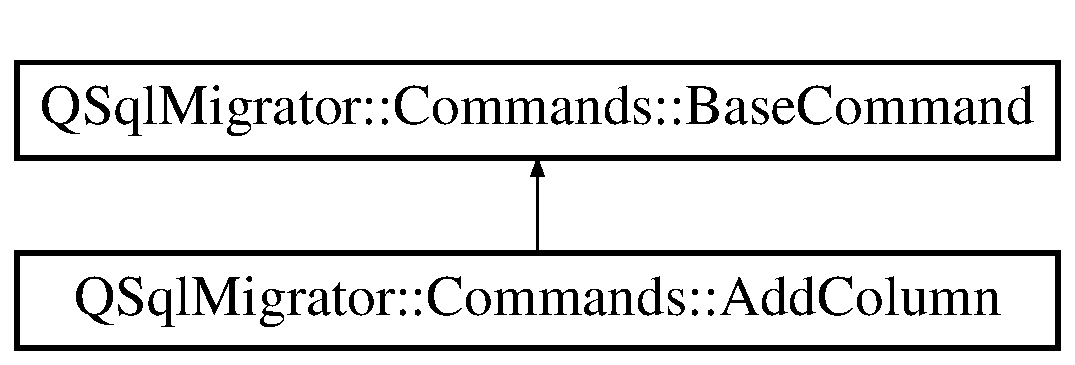
\includegraphics[height=2.000000cm]{class_q_sql_migrator_1_1_commands_1_1_add_column}
\end{center}
\end{figure}
\subsection*{Public Member Functions}
\begin{DoxyCompactItemize}
\item 
\mbox{\Hypertarget{class_q_sql_migrator_1_1_commands_1_1_add_column_a131604bb008e1dc369c54274a86ef7fa}\label{class_q_sql_migrator_1_1_commands_1_1_add_column_a131604bb008e1dc369c54274a86ef7fa}} 
{\bfseries Add\+Column} (const \hyperlink{class_q_sql_migrator_1_1_structure_1_1_column}{Structure\+::\+Column} \&column, const Q\+String \&table\+Name)
\item 
\mbox{\Hypertarget{class_q_sql_migrator_1_1_commands_1_1_add_column_a776e84c43628b22964438b9875e03b3b}\label{class_q_sql_migrator_1_1_commands_1_1_add_column_a776e84c43628b22964438b9875e03b3b}} 
const \hyperlink{class_q_sql_migrator_1_1_structure_1_1_column}{Structure\+::\+Column} \& {\bfseries column} () const
\item 
\mbox{\Hypertarget{class_q_sql_migrator_1_1_commands_1_1_add_column_afc7ad789564decdaadfdcd434a9bc842}\label{class_q_sql_migrator_1_1_commands_1_1_add_column_afc7ad789564decdaadfdcd434a9bc842}} 
const Q\+String \& {\bfseries table\+Name} () const
\item 
\mbox{\Hypertarget{class_q_sql_migrator_1_1_commands_1_1_add_column_a78a9cc887121b5386af5167762083600}\label{class_q_sql_migrator_1_1_commands_1_1_add_column_a78a9cc887121b5386af5167762083600}} 
Command\+Ptr {\bfseries reverse} () const Q\+\_\+\+D\+E\+C\+L\+\_\+\+O\+V\+E\+R\+R\+I\+DE
\end{DoxyCompactItemize}
\subsection*{Static Public Member Functions}
\begin{DoxyCompactItemize}
\item 
\mbox{\Hypertarget{class_q_sql_migrator_1_1_commands_1_1_add_column_a09150d0d578297e1444215f6a8a459aa}\label{class_q_sql_migrator_1_1_commands_1_1_add_column_a09150d0d578297e1444215f6a8a459aa}} 
static const Q\+String \& {\bfseries type\+Name} ()
\end{DoxyCompactItemize}


\subsection{Detailed Description}
value object representing the command to add a column to a table 

The documentation for this class was generated from the following files\+:\begin{DoxyCompactItemize}
\item 
/home/george/\+Develop/\+Praaline\+Py/praaline-\/core/\+Q\+Sql\+Migrator/\+Commands/Add\+Column.\+h\item 
/home/george/\+Develop/\+Praaline\+Py/praaline-\/core/\+Q\+Sql\+Migrator/\+Commands/Add\+Column.\+cpp\end{DoxyCompactItemize}

\hypertarget{class_q_sql_migrator_1_1_commands_1_1_alter_column_type}{}\section{Q\+Sql\+Migrator\+:\+:Commands\+:\+:Alter\+Column\+Type Class Reference}
\label{class_q_sql_migrator_1_1_commands_1_1_alter_column_type}\index{Q\+Sql\+Migrator\+::\+Commands\+::\+Alter\+Column\+Type@{Q\+Sql\+Migrator\+::\+Commands\+::\+Alter\+Column\+Type}}


value object representing the command to alter the type of a column in a table  




{\ttfamily \#include $<$Alter\+Column\+Type.\+h$>$}

Inheritance diagram for Q\+Sql\+Migrator\+:\+:Commands\+:\+:Alter\+Column\+Type\+:\begin{figure}[H]
\begin{center}
\leavevmode
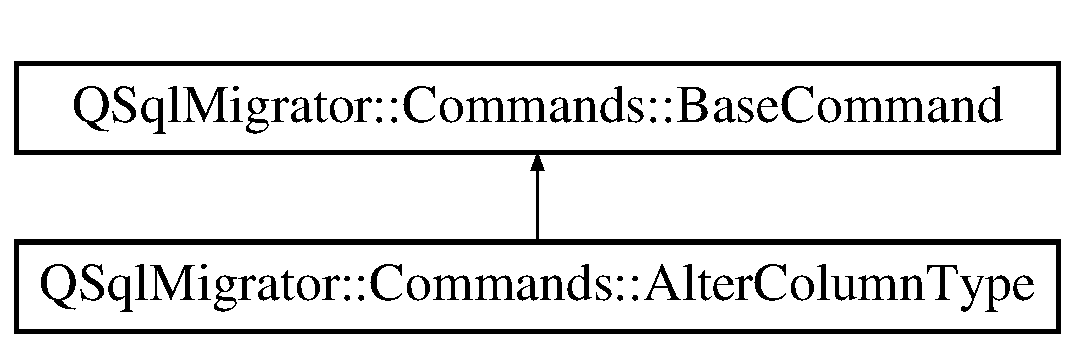
\includegraphics[height=2.000000cm]{class_q_sql_migrator_1_1_commands_1_1_alter_column_type}
\end{center}
\end{figure}
\subsection*{Public Member Functions}
\begin{DoxyCompactItemize}
\item 
\mbox{\Hypertarget{class_q_sql_migrator_1_1_commands_1_1_alter_column_type_a389a84f882f834feb2f8bc39ac1a52b8}\label{class_q_sql_migrator_1_1_commands_1_1_alter_column_type_a389a84f882f834feb2f8bc39ac1a52b8}} 
{\bfseries Alter\+Column\+Type} (const Q\+String \&column\+Name, const Q\+String \&table\+Name, const \hyperlink{class_q_sql_migrator_1_1_structure_1_1_sql_type}{Structure\+::\+Sql\+Type} \&new\+Type, const \hyperlink{class_q_sql_migrator_1_1_structure_1_1_sql_type}{Structure\+::\+Sql\+Type} \&old\+Type)
\item 
\mbox{\Hypertarget{class_q_sql_migrator_1_1_commands_1_1_alter_column_type_af1ea88e297e57ea86738f177353dcc19}\label{class_q_sql_migrator_1_1_commands_1_1_alter_column_type_af1ea88e297e57ea86738f177353dcc19}} 
{\bfseries Alter\+Column\+Type} (const Q\+String \&column\+Name, const Q\+String \&table\+Name, const \hyperlink{class_q_sql_migrator_1_1_structure_1_1_sql_type}{Structure\+::\+Sql\+Type} \&new\+Type)
\item 
\mbox{\Hypertarget{class_q_sql_migrator_1_1_commands_1_1_alter_column_type_aabc82e499fd27ec477de757e43526b0c}\label{class_q_sql_migrator_1_1_commands_1_1_alter_column_type_aabc82e499fd27ec477de757e43526b0c}} 
const Q\+String \& {\bfseries table\+Name} () const
\item 
\mbox{\Hypertarget{class_q_sql_migrator_1_1_commands_1_1_alter_column_type_ad49f44328b5043e3d0ac17e758d7b427}\label{class_q_sql_migrator_1_1_commands_1_1_alter_column_type_ad49f44328b5043e3d0ac17e758d7b427}} 
const Q\+String \& {\bfseries column\+Name} () const
\item 
\mbox{\Hypertarget{class_q_sql_migrator_1_1_commands_1_1_alter_column_type_a68536ff70a4a6316d10e88ae75dc48bf}\label{class_q_sql_migrator_1_1_commands_1_1_alter_column_type_a68536ff70a4a6316d10e88ae75dc48bf}} 
const \hyperlink{class_q_sql_migrator_1_1_structure_1_1_sql_type}{Structure\+::\+Sql\+Type} \& {\bfseries new\+Type} () const
\item 
\mbox{\Hypertarget{class_q_sql_migrator_1_1_commands_1_1_alter_column_type_aac6b416018cd712788934c3768e8d9cc}\label{class_q_sql_migrator_1_1_commands_1_1_alter_column_type_aac6b416018cd712788934c3768e8d9cc}} 
const \hyperlink{class_q_sql_migrator_1_1_structure_1_1_sql_type}{Structure\+::\+Sql\+Type} \& {\bfseries old\+Type} () const
\item 
\mbox{\Hypertarget{class_q_sql_migrator_1_1_commands_1_1_alter_column_type_a7c1bd7add836319bb47a184771c22f31}\label{class_q_sql_migrator_1_1_commands_1_1_alter_column_type_a7c1bd7add836319bb47a184771c22f31}} 
Command\+Ptr {\bfseries reverse} () const Q\+\_\+\+D\+E\+C\+L\+\_\+\+O\+V\+E\+R\+R\+I\+DE
\end{DoxyCompactItemize}
\subsection*{Static Public Member Functions}
\begin{DoxyCompactItemize}
\item 
\mbox{\Hypertarget{class_q_sql_migrator_1_1_commands_1_1_alter_column_type_a92f44cac5b0b3ba9dad1f6dd515e1886}\label{class_q_sql_migrator_1_1_commands_1_1_alter_column_type_a92f44cac5b0b3ba9dad1f6dd515e1886}} 
static const Q\+String \& {\bfseries type\+Name} ()
\end{DoxyCompactItemize}


\subsection{Detailed Description}
value object representing the command to alter the type of a column in a table 

The documentation for this class was generated from the following files\+:\begin{DoxyCompactItemize}
\item 
/home/george/\+Develop/\+Praaline\+Py/praaline-\/core/\+Q\+Sql\+Migrator/\+Commands/Alter\+Column\+Type.\+h\item 
/home/george/\+Develop/\+Praaline\+Py/praaline-\/core/\+Q\+Sql\+Migrator/\+Commands/Alter\+Column\+Type.\+cpp\end{DoxyCompactItemize}

\hypertarget{class_annotation_datastore}{}\section{Annotation\+Datastore Class Reference}
\label{class_annotation_datastore}\index{Annotation\+Datastore@{Annotation\+Datastore}}
Inheritance diagram for Annotation\+Datastore\+:\begin{figure}[H]
\begin{center}
\leavevmode
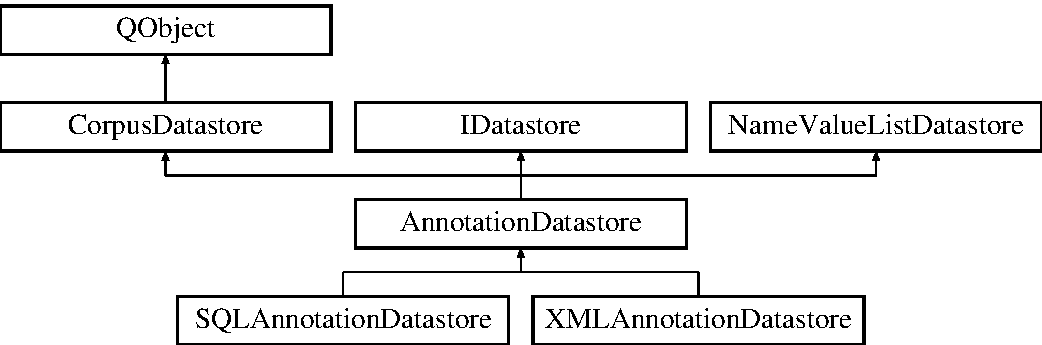
\includegraphics[height=4.000000cm]{class_annotation_datastore}
\end{center}
\end{figure}
\subsection*{Classes}
\begin{DoxyCompactItemize}
\item 
class \hyperlink{class_annotation_datastore_1_1_selection}{Selection}
\end{DoxyCompactItemize}
\subsection*{Public Member Functions}
\begin{DoxyCompactItemize}
\item 
\mbox{\Hypertarget{class_annotation_datastore_a7236e3eb5f39496f04501c0b52c1a7ea}\label{class_annotation_datastore_a7236e3eb5f39496f04501c0b52c1a7ea}} 
{\bfseries Annotation\+Datastore} (\hyperlink{class_corpus_repository}{Corpus\+Repository} $\ast$repository, Q\+Object $\ast$parent=nullptr)
\item 
\mbox{\Hypertarget{class_annotation_datastore_a859f9c1852d1b8926aed7a1783ae8e46}\label{class_annotation_datastore_a859f9c1852d1b8926aed7a1783ae8e46}} 
virtual bool {\bfseries create\+Datastore} (const \hyperlink{class_datastore_info}{Datastore\+Info} \&info)=0
\item 
\mbox{\Hypertarget{class_annotation_datastore_afb514e9043387c27e31f6696c7d8a1a9}\label{class_annotation_datastore_afb514e9043387c27e31f6696c7d8a1a9}} 
virtual bool {\bfseries open\+Datastore} (const \hyperlink{class_datastore_info}{Datastore\+Info} \&info)=0
\item 
\mbox{\Hypertarget{class_annotation_datastore_a03a3a2339a362a4bfa2167386c5309d8}\label{class_annotation_datastore_a03a3a2339a362a4bfa2167386c5309d8}} 
virtual bool {\bfseries close\+Datastore} ()=0
\item 
\mbox{\Hypertarget{class_annotation_datastore_a0653d5ceed01c982248f85cc8a167925}\label{class_annotation_datastore_a0653d5ceed01c982248f85cc8a167925}} 
virtual bool {\bfseries load\+Annotation\+Structure} ()=0
\item 
\mbox{\Hypertarget{class_annotation_datastore_a20fc685cb76fb6df83b5f457c61d21f9}\label{class_annotation_datastore_a20fc685cb76fb6df83b5f457c61d21f9}} 
virtual bool {\bfseries save\+Annotation\+Structure} ()=0
\item 
\mbox{\Hypertarget{class_annotation_datastore_a0275ed62dcaacf19c2fbd77776b7a8df}\label{class_annotation_datastore_a0275ed62dcaacf19c2fbd77776b7a8df}} 
virtual bool {\bfseries create\+Annotation\+Level} (\hyperlink{class_annotation_structure_level}{Annotation\+Structure\+Level} $\ast$new\+Level)=0
\item 
\mbox{\Hypertarget{class_annotation_datastore_aa90102ec514fd09d24516206bd1c0214}\label{class_annotation_datastore_aa90102ec514fd09d24516206bd1c0214}} 
virtual bool {\bfseries rename\+Annotation\+Level} (const Q\+String \&level\+ID, const Q\+String \&new\+Level\+ID)=0
\item 
\mbox{\Hypertarget{class_annotation_datastore_a0fc45673ff4f7e4c0604cf579ab00ea9}\label{class_annotation_datastore_a0fc45673ff4f7e4c0604cf579ab00ea9}} 
virtual bool {\bfseries delete\+Annotation\+Level} (const Q\+String \&level\+ID)=0
\item 
\mbox{\Hypertarget{class_annotation_datastore_aa0c8d67d5fa7f6389ec49431a5007082}\label{class_annotation_datastore_aa0c8d67d5fa7f6389ec49431a5007082}} 
virtual bool {\bfseries create\+Annotation\+Attribute} (const Q\+String \&level\+ID, \hyperlink{class_annotation_structure_attribute}{Annotation\+Structure\+Attribute} $\ast$new\+Attribute)=0
\item 
\mbox{\Hypertarget{class_annotation_datastore_ac9acf89fc8a6bbe69a92065c0511aceb}\label{class_annotation_datastore_ac9acf89fc8a6bbe69a92065c0511aceb}} 
virtual bool {\bfseries rename\+Annotation\+Attribute} (const Q\+String \&level\+ID, const Q\+String \&attribute\+ID, const Q\+String \&new\+Attribute\+ID)=0
\item 
\mbox{\Hypertarget{class_annotation_datastore_af69e5a5769239562d26ceb65b861dbbd}\label{class_annotation_datastore_af69e5a5769239562d26ceb65b861dbbd}} 
virtual bool {\bfseries delete\+Annotation\+Attribute} (const Q\+String \&level\+ID, const Q\+String \&attribute\+ID)=0
\item 
\mbox{\Hypertarget{class_annotation_datastore_a3fc607b737437f56ab99fbdc5f93eea3}\label{class_annotation_datastore_a3fc607b737437f56ab99fbdc5f93eea3}} 
virtual bool {\bfseries retype\+Annotation\+Attribute} (const Q\+String \&level\+ID, const Q\+String \&attribute\+ID, const \hyperlink{class_data_type}{Data\+Type} \&new\+Datatype)=0
\item 
\mbox{\Hypertarget{class_annotation_datastore_abec36f7893416d7bd948a49ebea82ddd}\label{class_annotation_datastore_abec36f7893416d7bd948a49ebea82ddd}} 
virtual \hyperlink{class_name_value_list}{Name\+Value\+List} $\ast$ {\bfseries get\+Name\+Value\+List} (const Q\+String \&list\+ID)=0
\item 
\mbox{\Hypertarget{class_annotation_datastore_acd6544544bf73139e5167259bb7cf9fa}\label{class_annotation_datastore_acd6544544bf73139e5167259bb7cf9fa}} 
virtual Q\+String\+List {\bfseries get\+All\+Name\+Value\+List\+I\+Ds} ()=0
\item 
\mbox{\Hypertarget{class_annotation_datastore_aa420f9a710d03b74219f370bc76bafd6}\label{class_annotation_datastore_aa420f9a710d03b74219f370bc76bafd6}} 
virtual Q\+Map$<$ Q\+String, Q\+Pointer$<$ \hyperlink{class_name_value_list}{Name\+Value\+List} $>$ $>$ {\bfseries get\+All\+Name\+Value\+Lists} ()=0
\item 
\mbox{\Hypertarget{class_annotation_datastore_a9adc754e4071980dc0e7026a6b7ed3f0}\label{class_annotation_datastore_a9adc754e4071980dc0e7026a6b7ed3f0}} 
virtual bool {\bfseries create\+Name\+Value\+List} (\hyperlink{class_name_value_list}{Name\+Value\+List} $\ast$list)=0
\item 
\mbox{\Hypertarget{class_annotation_datastore_ae06470eb992d4b88a7898a14db157e6e}\label{class_annotation_datastore_ae06470eb992d4b88a7898a14db157e6e}} 
virtual bool {\bfseries update\+Name\+Value\+List} (\hyperlink{class_name_value_list}{Name\+Value\+List} $\ast$list)=0
\item 
\mbox{\Hypertarget{class_annotation_datastore_a1cfb746ba61a9c126babd3d7dc903d07}\label{class_annotation_datastore_a1cfb746ba61a9c126babd3d7dc903d07}} 
virtual bool {\bfseries delete\+Name\+Value\+List} (const Q\+String \&list\+ID)=0
\item 
\mbox{\Hypertarget{class_annotation_datastore_ada50673875961000666ed8dcf4ea410b}\label{class_annotation_datastore_ada50673875961000666ed8dcf4ea410b}} 
virtual Q\+List$<$ \hyperlink{class_annotation_element}{Annotation\+Element} $\ast$ $>$ {\bfseries get\+Annotation\+Elements} (const \hyperlink{class_annotation_datastore_1_1_selection}{Selection} \&selection)=0
\item 
\mbox{\Hypertarget{class_annotation_datastore_afc48fd23fbd5e76832337d18d498ec23}\label{class_annotation_datastore_afc48fd23fbd5e76832337d18d498ec23}} 
virtual Q\+List$<$ \hyperlink{class_point}{Point} $\ast$ $>$ {\bfseries get\+Points} (const \hyperlink{class_annotation_datastore_1_1_selection}{Selection} \&selection)=0
\item 
\mbox{\Hypertarget{class_annotation_datastore_ad9d97f1d7b469bb6a3778db559b8156a}\label{class_annotation_datastore_ad9d97f1d7b469bb6a3778db559b8156a}} 
virtual Q\+List$<$ \hyperlink{class_interval}{Interval} $\ast$ $>$ {\bfseries get\+Intervals} (const \hyperlink{class_annotation_datastore_1_1_selection}{Selection} \&selection)=0
\item 
\mbox{\Hypertarget{class_annotation_datastore_a1021093e3313b9444b51470e96bb14ad}\label{class_annotation_datastore_a1021093e3313b9444b51470e96bb14ad}} 
virtual Q\+List$<$ \hyperlink{class_sequence}{Sequence} $\ast$ $>$ {\bfseries get\+Sequences} (const \hyperlink{class_annotation_datastore_1_1_selection}{Selection} \&selection)=0
\item 
\mbox{\Hypertarget{class_annotation_datastore_a61c96280f3fe6d8adc9024fb6a09a848}\label{class_annotation_datastore_a61c96280f3fe6d8adc9024fb6a09a848}} 
virtual bool {\bfseries save\+Annotation\+Elements} (const Q\+List$<$ \hyperlink{class_annotation_element}{Annotation\+Element} $\ast$$>$ \&elements, const Q\+String \&level\+ID, const Q\+String\+List \&attribute\+I\+Ds)=0
\item 
\mbox{\Hypertarget{class_annotation_datastore_a0d517fb11211e946fea7697fbce84760}\label{class_annotation_datastore_a0d517fb11211e946fea7697fbce84760}} 
virtual \hyperlink{class_annotation_tier}{Annotation\+Tier} $\ast$ {\bfseries get\+Tier} (const Q\+String \&annotation\+ID, const Q\+String \&speaker\+ID, const Q\+String \&level\+ID, const Q\+String\+List \&attribute\+I\+Ds=Q\+String\+List())=0
\item 
\mbox{\Hypertarget{class_annotation_datastore_af33579094950513253ac8fb8ce469cd4}\label{class_annotation_datastore_af33579094950513253ac8fb8ce469cd4}} 
virtual \hyperlink{class_annotation_tier_group}{Annotation\+Tier\+Group} $\ast$ {\bfseries get\+Tiers} (const Q\+String \&annotation\+ID, const Q\+String \&speaker\+ID, const Q\+String\+List \&level\+I\+Ds=Q\+String\+List())=0
\item 
\mbox{\Hypertarget{class_annotation_datastore_ac3a88f9754e4203d6d3fa69aab4a63ac}\label{class_annotation_datastore_ac3a88f9754e4203d6d3fa69aab4a63ac}} 
virtual Q\+Map$<$ Q\+String, Q\+Pointer$<$ \hyperlink{class_annotation_tier_group}{Annotation\+Tier\+Group} $>$ $>$ {\bfseries get\+Tiers\+All\+Speakers} (const Q\+String \&annotation\+ID, const Q\+String\+List \&level\+I\+Ds=Q\+String\+List())=0
\item 
\mbox{\Hypertarget{class_annotation_datastore_ac8b7d28bda28e35f8a010c0baabfa533}\label{class_annotation_datastore_ac8b7d28bda28e35f8a010c0baabfa533}} 
virtual bool {\bfseries save\+Tier} (const Q\+String \&annotation\+ID, const Q\+String \&speaker\+ID, \hyperlink{class_annotation_tier}{Annotation\+Tier} $\ast$tier)=0
\item 
\mbox{\Hypertarget{class_annotation_datastore_a1f58b42f870babfc061da7539b3e8230}\label{class_annotation_datastore_a1f58b42f870babfc061da7539b3e8230}} 
virtual bool {\bfseries save\+Tiers} (const Q\+String \&annotation\+ID, const Q\+String \&speaker\+ID, \hyperlink{class_annotation_tier_group}{Annotation\+Tier\+Group} $\ast$tiers)=0
\item 
\mbox{\Hypertarget{class_annotation_datastore_a3d1f231a8356c9bea95b85e447b575c9}\label{class_annotation_datastore_a3d1f231a8356c9bea95b85e447b575c9}} 
virtual bool {\bfseries save\+Tiers\+All\+Speakers} (const Q\+String \&annotation\+ID, Q\+Map$<$ Q\+String, Q\+Pointer$<$ \hyperlink{class_annotation_tier_group}{Annotation\+Tier\+Group} $>$ $>$ \&tiers\+All\+Speakers)=0
\item 
\mbox{\Hypertarget{class_annotation_datastore_a19bbae5e3244d89630e0d0076b9cd36d}\label{class_annotation_datastore_a19bbae5e3244d89630e0d0076b9cd36d}} 
virtual bool {\bfseries delete\+Tier} (const Q\+String \&annotation\+ID, const Q\+String \&speaker\+ID, const Q\+String \&level\+ID)=0
\item 
\mbox{\Hypertarget{class_annotation_datastore_a31e0af72910b1a1d61b4b9689737eba6}\label{class_annotation_datastore_a31e0af72910b1a1d61b4b9689737eba6}} 
virtual bool {\bfseries delete\+Tiers} (const Q\+String \&annotation\+ID, const Q\+String \&speaker\+ID, const Q\+String\+List \&level\+I\+Ds=Q\+String\+List())=0
\item 
\mbox{\Hypertarget{class_annotation_datastore_a982353479adbad6270e78cdd06a7f040}\label{class_annotation_datastore_a982353479adbad6270e78cdd06a7f040}} 
virtual bool {\bfseries delete\+All\+Tiers\+All\+Speakers} (const Q\+String \&annotation\+ID)=0
\item 
\mbox{\Hypertarget{class_annotation_datastore_aaf4d52e41ff0beda8d676eb602a006ee}\label{class_annotation_datastore_aaf4d52e41ff0beda8d676eb602a006ee}} 
virtual Q\+String\+List {\bfseries get\+Speakers\+In\+Level} (const Q\+String \&annotation\+ID, const Q\+String \&level\+ID)=0
\item 
\mbox{\Hypertarget{class_annotation_datastore_a43cc8d3d8faa41fb59986504df0870c7}\label{class_annotation_datastore_a43cc8d3d8faa41fb59986504df0870c7}} 
virtual Q\+String\+List {\bfseries get\+Speakers\+Active\+In\+Level} (const Q\+String \&annotation\+ID, const Q\+String \&level\+ID)=0
\item 
\mbox{\Hypertarget{class_annotation_datastore_a49b550cf14cfbcb4d0f8cda3eb53d389}\label{class_annotation_datastore_a49b550cf14cfbcb4d0f8cda3eb53d389}} 
virtual Q\+String\+List {\bfseries get\+Speakers\+In\+Annotation} (const Q\+String \&annotation\+ID)=0
\item 
\mbox{\Hypertarget{class_annotation_datastore_a734eae060d0f2fda239f95545c087546}\label{class_annotation_datastore_a734eae060d0f2fda239f95545c087546}} 
virtual Q\+String\+List {\bfseries get\+Speakers\+Active\+In\+Annotation} (const Q\+String \&annotation\+ID)=0
\item 
\mbox{\Hypertarget{class_annotation_datastore_a09ea34856a0dc1537b92af36ae5a9a04}\label{class_annotation_datastore_a09ea34856a0dc1537b92af36ae5a9a04}} 
virtual \hyperlink{class_interval_tier}{Interval\+Tier} $\ast$ {\bfseries get\+Speaker\+Timeline} (const Q\+String \&communication\+ID, const Q\+String \&annotation\+ID, const Q\+String \&level\+ID, bool detailed=false)=0
\item 
\mbox{\Hypertarget{class_annotation_datastore_a419f8eb857d748250a93c93778b3f627}\label{class_annotation_datastore_a419f8eb857d748250a93c93778b3f627}} 
virtual Q\+List$<$ \hyperlink{struct_query_occurrence_pointer}{Query\+Occurrence\+Pointer} $\ast$ $>$ {\bfseries run\+Query} (\hyperlink{class_query_definition}{Query\+Definition} $\ast$qdef)=0
\item 
\mbox{\Hypertarget{class_annotation_datastore_ab03c5171638a76047f02831a7d26f04e}\label{class_annotation_datastore_ab03c5171638a76047f02831a7d26f04e}} 
virtual \hyperlink{class_query_occurrence}{Query\+Occurrence} $\ast$ {\bfseries get\+Occurrence} (\hyperlink{struct_query_occurrence_pointer}{Query\+Occurrence\+Pointer} $\ast$pointer, \hyperlink{class_query_definition}{Query\+Definition} $\ast$qdef, int length\+Context\+Left=10, int length\+Context\+Right=10)=0
\item 
\mbox{\Hypertarget{class_annotation_datastore_aa159e0e4e9489f316432d08367e2e40e}\label{class_annotation_datastore_aa159e0e4e9489f316432d08367e2e40e}} 
virtual bool {\bfseries update\+Annotations\+From\+Query\+Occurrences} (const Q\+List$<$ \hyperlink{class_query_occurrence}{Query\+Occurrence} $\ast$$>$ \&occurrences)=0
\item 
\mbox{\Hypertarget{class_annotation_datastore_adb841a175d2d5c41324eeb89119d3b77}\label{class_annotation_datastore_adb841a175d2d5c41324eeb89119d3b77}} 
virtual Q\+List$<$ Q\+Pair$<$ Q\+List$<$ Q\+Variant $>$, long $>$ $>$ {\bfseries get\+Distinct\+Labels} (const Q\+String \&level\+ID, const Q\+String\+List \&attribute\+I\+Ds)=0
\item 
\mbox{\Hypertarget{class_annotation_datastore_a1e0e586fb9bdd8ed5a1c0e3158bb71c2}\label{class_annotation_datastore_a1e0e586fb9bdd8ed5a1c0e3158bb71c2}} 
virtual bool {\bfseries batch\+Update} (const Q\+String \&level\+ID, const Q\+String \&attribute\+ID, const Q\+Variant \&new\+Value, const Q\+List$<$ Q\+Pair$<$ Q\+String, Q\+Variant $>$ $>$ \&criteria)=0
\item 
\mbox{\Hypertarget{class_annotation_datastore_a12d810173b2245a21ef7090fc1298cba}\label{class_annotation_datastore_a12d810173b2245a21ef7090fc1298cba}} 
virtual Q\+List$<$ Q\+Pair$<$ Q\+List$<$ Q\+Variant $>$, long long $>$ $>$ {\bfseries count\+Items} (const Q\+String \&level\+ID, const Q\+String\+List \&group\+By\+Attribute\+I\+Ds, bool exclude\+N\+U\+LL, Q\+String\+List exclude\+Values)=0
\end{DoxyCompactItemize}
\subsection*{Additional Inherited Members}


The documentation for this class was generated from the following files\+:\begin{DoxyCompactItemize}
\item 
/home/george/\+Develop/\+Praaline\+Py/praaline-\/core/datastore/Annotation\+Datastore.\+h\item 
/home/george/\+Develop/\+Praaline\+Py/praaline-\/core/datastore/Annotation\+Datastore.\+cpp\end{DoxyCompactItemize}

\hypertarget{class_annotation_data_table}{}\section{Annotation\+Data\+Table Class Reference}
\label{class_annotation_data_table}\index{Annotation\+Data\+Table@{Annotation\+Data\+Table}}
Inheritance diagram for Annotation\+Data\+Table\+:\begin{figure}[H]
\begin{center}
\leavevmode
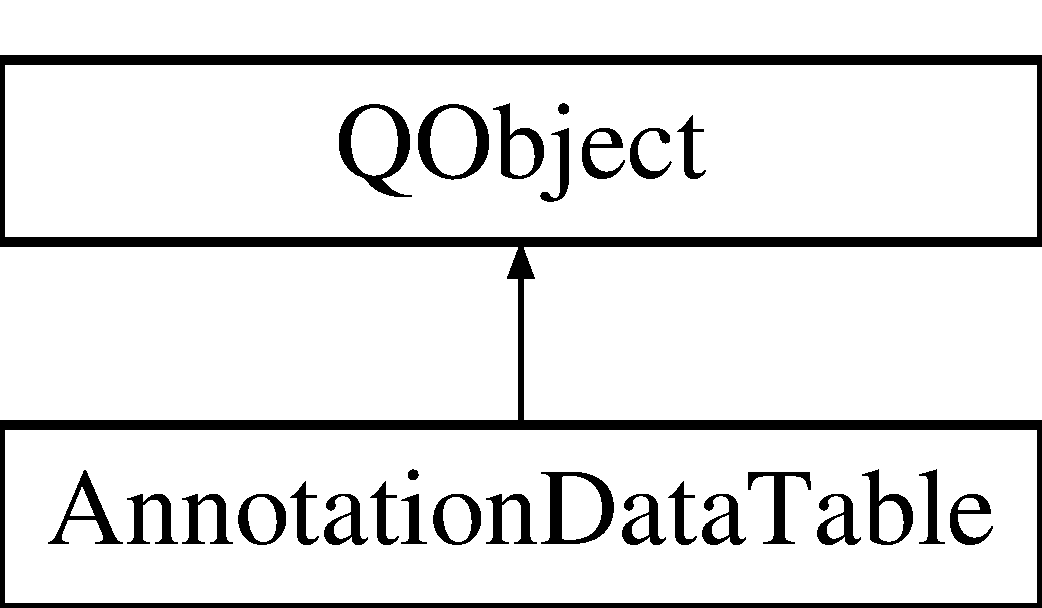
\includegraphics[height=2.000000cm]{class_annotation_data_table}
\end{center}
\end{figure}
\subsection*{Public Member Functions}
\begin{DoxyCompactItemize}
\item 
\mbox{\Hypertarget{class_annotation_data_table_a9cd8dbd5517223faf88738861592e1b2}\label{class_annotation_data_table_a9cd8dbd5517223faf88738861592e1b2}} 
{\bfseries Annotation\+Data\+Table} (Q\+Object $\ast$parent=nullptr)
\item 
\mbox{\Hypertarget{class_annotation_data_table_a3bb5fef5eb61006cc1def988971dd1a7}\label{class_annotation_data_table_a3bb5fef5eb61006cc1def988971dd1a7}} 
Q\+String {\bfseries ID} () const
\item 
\mbox{\Hypertarget{class_annotation_data_table_a0c3caeb053de8a836591e2fb1d44276e}\label{class_annotation_data_table_a0c3caeb053de8a836591e2fb1d44276e}} 
void {\bfseries set\+ID} (const Q\+String \&ID)
\item 
\mbox{\Hypertarget{class_annotation_data_table_aa83585d8e9a0f46217cef54e6edf34c8}\label{class_annotation_data_table_aa83585d8e9a0f46217cef54e6edf34c8}} 
virtual int {\bfseries get\+Row\+Count} () const
\item 
\mbox{\Hypertarget{class_annotation_data_table_ae615477727944e802d7c6a31a5b20fa3}\label{class_annotation_data_table_ae615477727944e802d7c6a31a5b20fa3}} 
virtual int {\bfseries get\+Column\+Count} () const
\item 
\mbox{\Hypertarget{class_annotation_data_table_affff74ce59813fc25d3bacdfd7fca8a7}\label{class_annotation_data_table_affff74ce59813fc25d3bacdfd7fca8a7}} 
virtual void {\bfseries clear} ()
\item 
\mbox{\Hypertarget{class_annotation_data_table_a83c2f39fe283c1a24143aa6081782c82}\label{class_annotation_data_table_a83c2f39fe283c1a24143aa6081782c82}} 
virtual Q\+String\+List {\bfseries get\+Field\+Names} () const
\item 
\mbox{\Hypertarget{class_annotation_data_table_ab5034b1e2e4ac003256e16c23f3c8ef4}\label{class_annotation_data_table_ab5034b1e2e4ac003256e16c23f3c8ef4}} 
virtual Q\+String\+List {\bfseries get\+Field\+Types} () const
\item 
\mbox{\Hypertarget{class_annotation_data_table_a61bfa44a0812926cfd0dfd8fcbf212aa}\label{class_annotation_data_table_a61bfa44a0812926cfd0dfd8fcbf212aa}} 
virtual Q\+String {\bfseries get\+Field\+Type} (const Q\+String \&fieldname) const
\item 
\mbox{\Hypertarget{class_annotation_data_table_ad1288d2aa7fe792846ff8ad3aa82e330}\label{class_annotation_data_table_ad1288d2aa7fe792846ff8ad3aa82e330}} 
virtual Q\+String\+List {\bfseries get\+Field\+Descriptions} () const
\item 
\mbox{\Hypertarget{class_annotation_data_table_a60a351378304306138282bf0abeaae49}\label{class_annotation_data_table_a60a351378304306138282bf0abeaae49}} 
virtual Q\+String {\bfseries get\+Field\+Description} (const Q\+String \&fieldname) const
\item 
\mbox{\Hypertarget{class_annotation_data_table_aca3b008ac804aa4161d535f8e156666e}\label{class_annotation_data_table_aca3b008ac804aa4161d535f8e156666e}} 
virtual Q\+Variant {\bfseries get\+Data} (int row, int column)
\item 
\mbox{\Hypertarget{class_annotation_data_table_a1668a4b81487d426455ae4991c98ee76}\label{class_annotation_data_table_a1668a4b81487d426455ae4991c98ee76}} 
virtual Q\+Variant {\bfseries get\+Data} (int row, const Q\+String \&fieldname)
\item 
\mbox{\Hypertarget{class_annotation_data_table_a21098ca0767b4271c09067a71a7816ad}\label{class_annotation_data_table_a21098ca0767b4271c09067a71a7816ad}} 
virtual \hyperlink{struct_real_time}{Real\+Time} {\bfseries get\+Seconds} (int row, const Q\+String \&fieldname)
\item 
\mbox{\Hypertarget{class_annotation_data_table_a8eabd054b682733828d77063c689c873}\label{class_annotation_data_table_a8eabd054b682733828d77063c689c873}} 
virtual bool {\bfseries read\+From\+File} (const Q\+String \&filename)
\item 
\mbox{\Hypertarget{class_annotation_data_table_a406d1a6f7cebcbd390a975bf06c61636}\label{class_annotation_data_table_a406d1a6f7cebcbd390a975bf06c61636}} 
virtual bool {\bfseries save\+To\+File} (const Q\+String \&filename)
\item 
\mbox{\Hypertarget{class_annotation_data_table_aa85289b28a3d6e5d9def64f899f95fc9}\label{class_annotation_data_table_aa85289b28a3d6e5d9def64f899f95fc9}} 
virtual \hyperlink{class_real_value_list}{Real\+Value\+List} {\bfseries get\+Value\+List} (const Q\+String \&fieldname)
\end{DoxyCompactItemize}
\subsection*{Protected Attributes}
\begin{DoxyCompactItemize}
\item 
\mbox{\Hypertarget{class_annotation_data_table_a37114464f331a0b7e5b6563efd1d00d1}\label{class_annotation_data_table_a37114464f331a0b7e5b6563efd1d00d1}} 
Q\+String {\bfseries m\+\_\+\+ID}
\item 
\mbox{\Hypertarget{class_annotation_data_table_acd1274d7181c721cb2fa6be4b3d479dc}\label{class_annotation_data_table_acd1274d7181c721cb2fa6be4b3d479dc}} 
Q\+Hash$<$ Q\+String, int $>$ {\bfseries m\+\_\+field\+Names}
\item 
\mbox{\Hypertarget{class_annotation_data_table_a6d9245d23b68a6f3f8caa32a8d29acf3}\label{class_annotation_data_table_a6d9245d23b68a6f3f8caa32a8d29acf3}} 
Q\+Hash$<$ Q\+String, Q\+String $>$ {\bfseries m\+\_\+field\+Types}
\item 
\mbox{\Hypertarget{class_annotation_data_table_a984a95fc42d98a02f272404676105b2f}\label{class_annotation_data_table_a984a95fc42d98a02f272404676105b2f}} 
Q\+Hash$<$ Q\+String, Q\+String $>$ {\bfseries m\+\_\+field\+Descriptions}
\item 
\mbox{\Hypertarget{class_annotation_data_table_aa69e33213d49a794b875c56e6335e5bd}\label{class_annotation_data_table_aa69e33213d49a794b875c56e6335e5bd}} 
Q\+List$<$ Q\+List$<$ Q\+Variant $>$ $>$ {\bfseries m\+\_\+data}
\end{DoxyCompactItemize}


The documentation for this class was generated from the following files\+:\begin{DoxyCompactItemize}
\item 
/home/george/\+Develop/\+Praaline\+Py/praaline-\/core/annotation/Annotation\+Data\+Table.\+h\item 
/home/george/\+Develop/\+Praaline\+Py/praaline-\/core/annotation/Annotation\+Data\+Table.\+cpp\end{DoxyCompactItemize}

\hypertarget{class_annotation_element}{}\section{Annotation\+Element Class Reference}
\label{class_annotation_element}\index{Annotation\+Element@{Annotation\+Element}}


The \hyperlink{class_annotation_element}{Annotation\+Element} class.  




{\ttfamily \#include $<$Annotation\+Element.\+h$>$}

Inheritance diagram for Annotation\+Element\+:\begin{figure}[H]
\begin{center}
\leavevmode
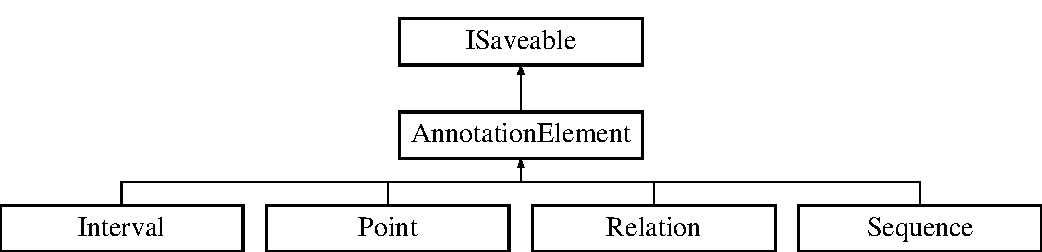
\includegraphics[height=3.000000cm]{class_annotation_element}
\end{center}
\end{figure}
\subsection*{Public Types}
\begin{DoxyCompactItemize}
\item 
\mbox{\Hypertarget{class_annotation_element_af5282990ffbe25eeea8ab02037e344b0}\label{class_annotation_element_af5282990ffbe25eeea8ab02037e344b0}} 
enum \hyperlink{class_annotation_element_af5282990ffbe25eeea8ab02037e344b0}{Element\+Type} \{ \newline
{\bfseries Type\+\_\+\+Element}, 
{\bfseries Type\+\_\+\+Point}, 
{\bfseries Type\+\_\+\+Interval}, 
{\bfseries Type\+\_\+\+Sequence}, 
\newline
{\bfseries Type\+\_\+\+Relation}
 \}\begin{DoxyCompactList}\small\item\em The Element\+Type enum. \end{DoxyCompactList}
\end{DoxyCompactItemize}
\subsection*{Public Member Functions}
\begin{DoxyCompactItemize}
\item 
\mbox{\Hypertarget{class_annotation_element_a8a7015a798a7b3dba1f55ab5482db2be}\label{class_annotation_element_a8a7015a798a7b3dba1f55ab5482db2be}} 
\hyperlink{class_annotation_element_a8a7015a798a7b3dba1f55ab5482db2be}{Annotation\+Element} ()
\begin{DoxyCompactList}\small\item\em \hyperlink{class_annotation_element}{Annotation\+Element}. \end{DoxyCompactList}\item 
\hyperlink{class_annotation_element_a77b837f3d7eb7d450b1aca83765a488f}{Annotation\+Element} (const Q\+String \&\hyperlink{class_annotation_element_aa59bd98501e3882990681f6aff2ee863}{text})
\begin{DoxyCompactList}\small\item\em \hyperlink{class_annotation_element}{Annotation\+Element}. \end{DoxyCompactList}\item 
\hyperlink{class_annotation_element_a12c2571e880beacafbceadb16b6bd0bb}{Annotation\+Element} (const Q\+String \&\hyperlink{class_annotation_element_aa59bd98501e3882990681f6aff2ee863}{text}, const Q\+Hash$<$ Q\+String, Q\+Variant $>$ \&\hyperlink{class_annotation_element_a58082d92f50c4fde2d18ce24ef3fd283}{attributes})
\begin{DoxyCompactList}\small\item\em \hyperlink{class_annotation_element}{Annotation\+Element}. \end{DoxyCompactList}\item 
\hyperlink{class_annotation_element_a9add1ee0c531f6b65743e691a42991fe}{Annotation\+Element} (const \hyperlink{class_annotation_element}{Annotation\+Element} \&other)
\begin{DoxyCompactList}\small\item\em \hyperlink{class_annotation_element}{Annotation\+Element}. \end{DoxyCompactList}\item 
\mbox{\Hypertarget{class_annotation_element_a289fc117206f35b038a4aaa5c335aba3}\label{class_annotation_element_a289fc117206f35b038a4aaa5c335aba3}} 
virtual \hyperlink{class_annotation_element_a289fc117206f35b038a4aaa5c335aba3}{$\sim$\+Annotation\+Element} () override
\begin{DoxyCompactList}\small\item\em $\sim$\+Annotation\+Element \end{DoxyCompactList}\item 
virtual \hyperlink{class_annotation_element_af5282990ffbe25eeea8ab02037e344b0}{Element\+Type} \hyperlink{class_annotation_element_a9b2d5cf05a2f81d9b2103a5c736dfb2d}{element\+Type} () const
\begin{DoxyCompactList}\small\item\em element\+Type \end{DoxyCompactList}\item 
virtual Q\+String \hyperlink{class_annotation_element_aa59bd98501e3882990681f6aff2ee863}{text} () const
\begin{DoxyCompactList}\small\item\em text \end{DoxyCompactList}\item 
virtual void \hyperlink{class_annotation_element_a67b28559349cd0ca84d47f629ee4ee45}{set\+Text} (const Q\+String \&\hyperlink{class_annotation_element_aa59bd98501e3882990681f6aff2ee863}{text})
\begin{DoxyCompactList}\small\item\em set\+Text \end{DoxyCompactList}\item 
virtual void \hyperlink{class_annotation_element_aefb0498f0c301d7c1f04ba2d32397f7c}{append\+Text} (const Q\+String \&appended\+Text)
\begin{DoxyCompactList}\small\item\em append\+Text \end{DoxyCompactList}\item 
virtual void \hyperlink{class_annotation_element_a6ea70bff6f981c1d6014579d4c7fc680}{replace\+Text} (const Q\+String \&before, const Q\+String \&after, Qt\+::\+Case\+Sensitivity cs=Qt\+::\+Case\+Sensitive)
\begin{DoxyCompactList}\small\item\em replace\+Text \end{DoxyCompactList}\item 
virtual void \hyperlink{class_annotation_element_aafa5f3ee2d42db969bafb453e16c35b3}{replace\+Attribute\+Text} (const Q\+String \&attribute\+ID, const Q\+String \&before, const Q\+String \&after, Qt\+::\+Case\+Sensitivity cs=Qt\+::\+Case\+Sensitive)
\begin{DoxyCompactList}\small\item\em replace\+Attribute\+Text \end{DoxyCompactList}\item 
virtual Q\+Variant \hyperlink{class_annotation_element_a55f85fb15ed52122653b0769c857899c}{attribute} (const Q\+String \&name) const
\begin{DoxyCompactList}\small\item\em attribute \end{DoxyCompactList}\item 
virtual void \hyperlink{class_annotation_element_a206d8790fe92a7c8e6b703d026836584}{set\+Attribute} (const Q\+String \&name, Q\+Variant value)
\begin{DoxyCompactList}\small\item\em set\+Attribute \end{DoxyCompactList}\item 
virtual void \hyperlink{class_annotation_element_a0acb66aa65f201880286d82dda4d82bf}{remove\+Attribute} (const Q\+String \&name)
\begin{DoxyCompactList}\small\item\em remove\+Attribute \end{DoxyCompactList}\item 
\mbox{\Hypertarget{class_annotation_element_af81f11a7d19f09e28a73cc3af49fd128}\label{class_annotation_element_af81f11a7d19f09e28a73cc3af49fd128}} 
virtual void \hyperlink{class_annotation_element_af81f11a7d19f09e28a73cc3af49fd128}{clear\+Attributes} ()
\begin{DoxyCompactList}\small\item\em clear\+Attributes \end{DoxyCompactList}\item 
virtual Q\+Hash$<$ Q\+String, Q\+Variant $>$ \hyperlink{class_annotation_element_a58082d92f50c4fde2d18ce24ef3fd283}{attributes} () const
\begin{DoxyCompactList}\small\item\em attributes \end{DoxyCompactList}\item 
virtual Q\+List$<$ Q\+String $>$ \hyperlink{class_annotation_element_ab28b90d83a5fdf7d150df32871f43ce8}{attribute\+Names} () const
\begin{DoxyCompactList}\small\item\em attribute\+Names \end{DoxyCompactList}\end{DoxyCompactItemize}
\subsection*{Protected Attributes}
\begin{DoxyCompactItemize}
\item 
\mbox{\Hypertarget{class_annotation_element_a4b8247dab4ac0617a86efeb83dd81b3d}\label{class_annotation_element_a4b8247dab4ac0617a86efeb83dd81b3d}} 
Q\+String {\bfseries m\+\_\+text}
\item 
\mbox{\Hypertarget{class_annotation_element_afb3291121c572b7f2a08f7cf866fa553}\label{class_annotation_element_afb3291121c572b7f2a08f7cf866fa553}} 
Q\+Variant\+Hash {\bfseries m\+\_\+attributes}
\end{DoxyCompactItemize}
\subsection*{Friends}
\begin{DoxyCompactItemize}
\item 
\mbox{\Hypertarget{class_annotation_element_a2a64bb821e0fcc1c90c808ce5a2eb6ef}\label{class_annotation_element_a2a64bb821e0fcc1c90c808ce5a2eb6ef}} 
class {\bfseries Annotation\+Tier}
\end{DoxyCompactItemize}


\subsection{Detailed Description}
The \hyperlink{class_annotation_element}{Annotation\+Element} class. 

\subsection{Constructor \& Destructor Documentation}
\mbox{\Hypertarget{class_annotation_element_a77b837f3d7eb7d450b1aca83765a488f}\label{class_annotation_element_a77b837f3d7eb7d450b1aca83765a488f}} 
\index{Annotation\+Element@{Annotation\+Element}!Annotation\+Element@{Annotation\+Element}}
\index{Annotation\+Element@{Annotation\+Element}!Annotation\+Element@{Annotation\+Element}}
\subsubsection{\texorpdfstring{Annotation\+Element()}{AnnotationElement()}\hspace{0.1cm}{\footnotesize\ttfamily [1/3]}}
{\footnotesize\ttfamily Annotation\+Element\+::\+Annotation\+Element (\begin{DoxyParamCaption}\item[{const Q\+String \&}]{text }\end{DoxyParamCaption})\hspace{0.3cm}{\ttfamily [explicit]}}



\hyperlink{class_annotation_element}{Annotation\+Element}. 


\begin{DoxyParams}{Parameters}
{\em text} & \\
\hline
\end{DoxyParams}
\mbox{\Hypertarget{class_annotation_element_a12c2571e880beacafbceadb16b6bd0bb}\label{class_annotation_element_a12c2571e880beacafbceadb16b6bd0bb}} 
\index{Annotation\+Element@{Annotation\+Element}!Annotation\+Element@{Annotation\+Element}}
\index{Annotation\+Element@{Annotation\+Element}!Annotation\+Element@{Annotation\+Element}}
\subsubsection{\texorpdfstring{Annotation\+Element()}{AnnotationElement()}\hspace{0.1cm}{\footnotesize\ttfamily [2/3]}}
{\footnotesize\ttfamily Annotation\+Element\+::\+Annotation\+Element (\begin{DoxyParamCaption}\item[{const Q\+String \&}]{text,  }\item[{const Q\+Hash$<$ Q\+String, Q\+Variant $>$ \&}]{attributes }\end{DoxyParamCaption})}



\hyperlink{class_annotation_element}{Annotation\+Element}. 


\begin{DoxyParams}{Parameters}
{\em text} & \\
\hline
{\em attributes} & \\
\hline
\end{DoxyParams}
\mbox{\Hypertarget{class_annotation_element_a9add1ee0c531f6b65743e691a42991fe}\label{class_annotation_element_a9add1ee0c531f6b65743e691a42991fe}} 
\index{Annotation\+Element@{Annotation\+Element}!Annotation\+Element@{Annotation\+Element}}
\index{Annotation\+Element@{Annotation\+Element}!Annotation\+Element@{Annotation\+Element}}
\subsubsection{\texorpdfstring{Annotation\+Element()}{AnnotationElement()}\hspace{0.1cm}{\footnotesize\ttfamily [3/3]}}
{\footnotesize\ttfamily Annotation\+Element\+::\+Annotation\+Element (\begin{DoxyParamCaption}\item[{const \hyperlink{class_annotation_element}{Annotation\+Element} \&}]{other }\end{DoxyParamCaption})}



\hyperlink{class_annotation_element}{Annotation\+Element}. 


\begin{DoxyParams}{Parameters}
{\em other} & \\
\hline
\end{DoxyParams}


\subsection{Member Function Documentation}
\mbox{\Hypertarget{class_annotation_element_aefb0498f0c301d7c1f04ba2d32397f7c}\label{class_annotation_element_aefb0498f0c301d7c1f04ba2d32397f7c}} 
\index{Annotation\+Element@{Annotation\+Element}!append\+Text@{append\+Text}}
\index{append\+Text@{append\+Text}!Annotation\+Element@{Annotation\+Element}}
\subsubsection{\texorpdfstring{append\+Text()}{appendText()}}
{\footnotesize\ttfamily virtual void Annotation\+Element\+::append\+Text (\begin{DoxyParamCaption}\item[{const Q\+String \&}]{appended\+Text }\end{DoxyParamCaption})\hspace{0.3cm}{\ttfamily [inline]}, {\ttfamily [virtual]}}



append\+Text 


\begin{DoxyParams}{Parameters}
{\em appended\+Text} & \\
\hline
\end{DoxyParams}
\mbox{\Hypertarget{class_annotation_element_a55f85fb15ed52122653b0769c857899c}\label{class_annotation_element_a55f85fb15ed52122653b0769c857899c}} 
\index{Annotation\+Element@{Annotation\+Element}!attribute@{attribute}}
\index{attribute@{attribute}!Annotation\+Element@{Annotation\+Element}}
\subsubsection{\texorpdfstring{attribute()}{attribute()}}
{\footnotesize\ttfamily virtual Q\+Variant Annotation\+Element\+::attribute (\begin{DoxyParamCaption}\item[{const Q\+String \&}]{name }\end{DoxyParamCaption}) const\hspace{0.3cm}{\ttfamily [inline]}, {\ttfamily [virtual]}}



attribute 


\begin{DoxyParams}{Parameters}
{\em name} & \\
\hline
\end{DoxyParams}
\begin{DoxyReturn}{Returns}

\end{DoxyReturn}


Reimplemented in \hyperlink{class_interval_aebcaee36c1adf49669d8a0faa16a335f}{Interval}, \hyperlink{class_sequence_a415f655b5985fa47499a7f665ce7c2d4}{Sequence}, \hyperlink{class_relation_a424ac3f46c1a62f2f72592dcf10d1f1e}{Relation}, and \hyperlink{class_point_a0ff561e393cdf7475126b96de6106d12}{Point}.

\mbox{\Hypertarget{class_annotation_element_ab28b90d83a5fdf7d150df32871f43ce8}\label{class_annotation_element_ab28b90d83a5fdf7d150df32871f43ce8}} 
\index{Annotation\+Element@{Annotation\+Element}!attribute\+Names@{attribute\+Names}}
\index{attribute\+Names@{attribute\+Names}!Annotation\+Element@{Annotation\+Element}}
\subsubsection{\texorpdfstring{attribute\+Names()}{attributeNames()}}
{\footnotesize\ttfamily virtual Q\+List$<$Q\+String$>$ Annotation\+Element\+::attribute\+Names (\begin{DoxyParamCaption}{ }\end{DoxyParamCaption}) const\hspace{0.3cm}{\ttfamily [inline]}, {\ttfamily [virtual]}}



attribute\+Names 

\begin{DoxyReturn}{Returns}

\end{DoxyReturn}
\mbox{\Hypertarget{class_annotation_element_a58082d92f50c4fde2d18ce24ef3fd283}\label{class_annotation_element_a58082d92f50c4fde2d18ce24ef3fd283}} 
\index{Annotation\+Element@{Annotation\+Element}!attributes@{attributes}}
\index{attributes@{attributes}!Annotation\+Element@{Annotation\+Element}}
\subsubsection{\texorpdfstring{attributes()}{attributes()}}
{\footnotesize\ttfamily virtual Q\+Hash$<$Q\+String, Q\+Variant$>$ Annotation\+Element\+::attributes (\begin{DoxyParamCaption}{ }\end{DoxyParamCaption}) const\hspace{0.3cm}{\ttfamily [inline]}, {\ttfamily [virtual]}}



attributes 

\begin{DoxyReturn}{Returns}

\end{DoxyReturn}
\mbox{\Hypertarget{class_annotation_element_a9b2d5cf05a2f81d9b2103a5c736dfb2d}\label{class_annotation_element_a9b2d5cf05a2f81d9b2103a5c736dfb2d}} 
\index{Annotation\+Element@{Annotation\+Element}!element\+Type@{element\+Type}}
\index{element\+Type@{element\+Type}!Annotation\+Element@{Annotation\+Element}}
\subsubsection{\texorpdfstring{element\+Type()}{elementType()}}
{\footnotesize\ttfamily virtual \hyperlink{class_annotation_element_af5282990ffbe25eeea8ab02037e344b0}{Element\+Type} Annotation\+Element\+::element\+Type (\begin{DoxyParamCaption}{ }\end{DoxyParamCaption}) const\hspace{0.3cm}{\ttfamily [inline]}, {\ttfamily [virtual]}}



element\+Type 

\begin{DoxyReturn}{Returns}

\end{DoxyReturn}


Reimplemented in \hyperlink{class_interval_a3ea5342504df09262d59cd2ab1658804}{Interval}, \hyperlink{class_sequence_a09f57e396cbb4a9de8caa81ca3b96ad1}{Sequence}, \hyperlink{class_relation_a31e74e5707090aedfa225289b06683f4}{Relation}, and \hyperlink{class_point_ac576e4660a79cf5bbffa4591a22d2a28}{Point}.

\mbox{\Hypertarget{class_annotation_element_a0acb66aa65f201880286d82dda4d82bf}\label{class_annotation_element_a0acb66aa65f201880286d82dda4d82bf}} 
\index{Annotation\+Element@{Annotation\+Element}!remove\+Attribute@{remove\+Attribute}}
\index{remove\+Attribute@{remove\+Attribute}!Annotation\+Element@{Annotation\+Element}}
\subsubsection{\texorpdfstring{remove\+Attribute()}{removeAttribute()}}
{\footnotesize\ttfamily virtual void Annotation\+Element\+::remove\+Attribute (\begin{DoxyParamCaption}\item[{const Q\+String \&}]{name }\end{DoxyParamCaption})\hspace{0.3cm}{\ttfamily [inline]}, {\ttfamily [virtual]}}



remove\+Attribute 


\begin{DoxyParams}{Parameters}
{\em name} & \\
\hline
\end{DoxyParams}
\mbox{\Hypertarget{class_annotation_element_aafa5f3ee2d42db969bafb453e16c35b3}\label{class_annotation_element_aafa5f3ee2d42db969bafb453e16c35b3}} 
\index{Annotation\+Element@{Annotation\+Element}!replace\+Attribute\+Text@{replace\+Attribute\+Text}}
\index{replace\+Attribute\+Text@{replace\+Attribute\+Text}!Annotation\+Element@{Annotation\+Element}}
\subsubsection{\texorpdfstring{replace\+Attribute\+Text()}{replaceAttributeText()}}
{\footnotesize\ttfamily virtual void Annotation\+Element\+::replace\+Attribute\+Text (\begin{DoxyParamCaption}\item[{const Q\+String \&}]{attribute\+ID,  }\item[{const Q\+String \&}]{before,  }\item[{const Q\+String \&}]{after,  }\item[{Qt\+::\+Case\+Sensitivity}]{cs = {\ttfamily Qt\+:\+:CaseSensitive} }\end{DoxyParamCaption})\hspace{0.3cm}{\ttfamily [inline]}, {\ttfamily [virtual]}}



replace\+Attribute\+Text 


\begin{DoxyParams}{Parameters}
{\em attribute\+ID} & \\
\hline
{\em before} & \\
\hline
{\em after} & \\
\hline
{\em cs} & \\
\hline
\end{DoxyParams}
\mbox{\Hypertarget{class_annotation_element_a6ea70bff6f981c1d6014579d4c7fc680}\label{class_annotation_element_a6ea70bff6f981c1d6014579d4c7fc680}} 
\index{Annotation\+Element@{Annotation\+Element}!replace\+Text@{replace\+Text}}
\index{replace\+Text@{replace\+Text}!Annotation\+Element@{Annotation\+Element}}
\subsubsection{\texorpdfstring{replace\+Text()}{replaceText()}}
{\footnotesize\ttfamily virtual void Annotation\+Element\+::replace\+Text (\begin{DoxyParamCaption}\item[{const Q\+String \&}]{before,  }\item[{const Q\+String \&}]{after,  }\item[{Qt\+::\+Case\+Sensitivity}]{cs = {\ttfamily Qt\+:\+:CaseSensitive} }\end{DoxyParamCaption})\hspace{0.3cm}{\ttfamily [inline]}, {\ttfamily [virtual]}}



replace\+Text 


\begin{DoxyParams}{Parameters}
{\em before} & \\
\hline
{\em after} & \\
\hline
{\em cs} & \\
\hline
\end{DoxyParams}
\mbox{\Hypertarget{class_annotation_element_a206d8790fe92a7c8e6b703d026836584}\label{class_annotation_element_a206d8790fe92a7c8e6b703d026836584}} 
\index{Annotation\+Element@{Annotation\+Element}!set\+Attribute@{set\+Attribute}}
\index{set\+Attribute@{set\+Attribute}!Annotation\+Element@{Annotation\+Element}}
\subsubsection{\texorpdfstring{set\+Attribute()}{setAttribute()}}
{\footnotesize\ttfamily virtual void Annotation\+Element\+::set\+Attribute (\begin{DoxyParamCaption}\item[{const Q\+String \&}]{name,  }\item[{Q\+Variant}]{value }\end{DoxyParamCaption})\hspace{0.3cm}{\ttfamily [inline]}, {\ttfamily [virtual]}}



set\+Attribute 


\begin{DoxyParams}{Parameters}
{\em name} & \\
\hline
{\em value} & \\
\hline
\end{DoxyParams}


Reimplemented in \hyperlink{class_interval_a0895204effc21e1f4ead9b78b4b9726f}{Interval}, \hyperlink{class_sequence_a0c573124c566aa3a28c63fb362f58c6b}{Sequence}, \hyperlink{class_relation_ae669645f5fc531a6118d68b51a4d64df}{Relation}, and \hyperlink{class_point_a997cc0d524866e257f58ef9a3e82a432}{Point}.

\mbox{\Hypertarget{class_annotation_element_a67b28559349cd0ca84d47f629ee4ee45}\label{class_annotation_element_a67b28559349cd0ca84d47f629ee4ee45}} 
\index{Annotation\+Element@{Annotation\+Element}!set\+Text@{set\+Text}}
\index{set\+Text@{set\+Text}!Annotation\+Element@{Annotation\+Element}}
\subsubsection{\texorpdfstring{set\+Text()}{setText()}}
{\footnotesize\ttfamily virtual void Annotation\+Element\+::set\+Text (\begin{DoxyParamCaption}\item[{const Q\+String \&}]{text }\end{DoxyParamCaption})\hspace{0.3cm}{\ttfamily [inline]}, {\ttfamily [virtual]}}



set\+Text 


\begin{DoxyParams}{Parameters}
{\em text} & \\
\hline
\end{DoxyParams}
\mbox{\Hypertarget{class_annotation_element_aa59bd98501e3882990681f6aff2ee863}\label{class_annotation_element_aa59bd98501e3882990681f6aff2ee863}} 
\index{Annotation\+Element@{Annotation\+Element}!text@{text}}
\index{text@{text}!Annotation\+Element@{Annotation\+Element}}
\subsubsection{\texorpdfstring{text()}{text()}}
{\footnotesize\ttfamily virtual Q\+String Annotation\+Element\+::text (\begin{DoxyParamCaption}{ }\end{DoxyParamCaption}) const\hspace{0.3cm}{\ttfamily [inline]}, {\ttfamily [virtual]}}



text 

\begin{DoxyReturn}{Returns}

\end{DoxyReturn}


The documentation for this class was generated from the following files\+:\begin{DoxyCompactItemize}
\item 
/home/george/\+Develop/\+Praaline\+Py/praaline-\/core/annotation/Annotation\+Element.\+h\item 
/home/george/\+Develop/\+Praaline\+Py/praaline-\/core/annotation/Annotation\+Element.\+cpp\end{DoxyCompactItemize}

\hypertarget{class_annotation_interface_praat}{}\section{Annotation\+Interface\+Praat Class Reference}
\label{class_annotation_interface_praat}\index{Annotation\+Interface\+Praat@{Annotation\+Interface\+Praat}}
Inheritance diagram for Annotation\+Interface\+Praat\+:\begin{figure}[H]
\begin{center}
\leavevmode
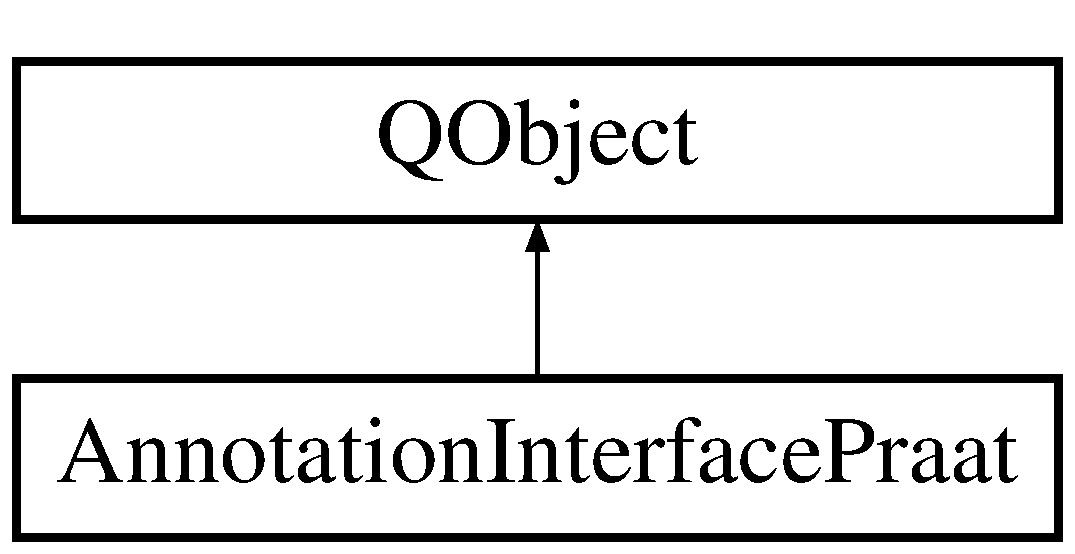
\includegraphics[height=2.000000cm]{class_annotation_interface_praat}
\end{center}
\end{figure}
\subsection*{Classes}
\begin{DoxyCompactItemize}
\item 
class \hyperlink{class_annotation_interface_praat_1_1_correspondance}{Correspondance}
\end{DoxyCompactItemize}
\subsection*{Public Types}
\begin{DoxyCompactItemize}
\item 
\mbox{\Hypertarget{class_annotation_interface_praat_a273453400af61ae2fcc5a7b9c1159ed3}\label{class_annotation_interface_praat_a273453400af61ae2fcc5a7b9c1159ed3}} 
enum {\bfseries Speaker\+Policy} \{ {\bfseries Speaker\+Policy\+\_\+\+Single\+Per\+File}, 
{\bfseries Speaker\+Policy\+\_\+\+Prefix\+Tier\+Names}, 
{\bfseries Speaker\+Policy\+\_\+\+Speaker\+Intervals}, 
{\bfseries Speaker\+Policy\+\_\+\+Primary\+And\+Secondary}
 \}
\end{DoxyCompactItemize}
\subsection*{Public Member Functions}
\begin{DoxyCompactItemize}
\item 
\mbox{\Hypertarget{class_annotation_interface_praat_a742fd0b5a46159d7d9ccde87729ba878}\label{class_annotation_interface_praat_a742fd0b5a46159d7d9ccde87729ba878}} 
{\bfseries Annotation\+Interface\+Praat} (Q\+Object $\ast$parent=nullptr)
\item 
\mbox{\Hypertarget{class_annotation_interface_praat_a6d487efc89a9d444c6a11852c4e68243}\label{class_annotation_interface_praat_a6d487efc89a9d444c6a11852c4e68243}} 
const Q\+List$<$ \hyperlink{class_annotation_interface_praat_1_1_correspondance}{Correspondance} $>$ \& {\bfseries correpondances} ()
\item 
\mbox{\Hypertarget{class_annotation_interface_praat_a3929379280fe84709cee5e85e63ab5dc}\label{class_annotation_interface_praat_a3929379280fe84709cee5e85e63ab5dc}} 
void {\bfseries add\+Correpondance} (const Q\+String \&level\+ID, const Q\+String \&attribute\+ID, const Q\+String \&tier\+Name)
\item 
\mbox{\Hypertarget{class_annotation_interface_praat_a1fcd0aa76675e6a6cbd5f0ae434755d8}\label{class_annotation_interface_praat_a1fcd0aa76675e6a6cbd5f0ae434755d8}} 
void {\bfseries remove\+Correpondance} (const Q\+String \&level\+ID, const Q\+String \&annotation\+ID)
\item 
\mbox{\Hypertarget{class_annotation_interface_praat_a31e83b4a9cd6ab92a63509473e07346e}\label{class_annotation_interface_praat_a31e83b4a9cd6ab92a63509473e07346e}} 
Speaker\+Policy {\bfseries speaker\+Policy} () const
\item 
\mbox{\Hypertarget{class_annotation_interface_praat_a0ae5a22c03e93422d87741b64d672677}\label{class_annotation_interface_praat_a0ae5a22c03e93422d87741b64d672677}} 
void {\bfseries set\+Speaker\+Policy} (Speaker\+Policy policy)
\item 
\mbox{\Hypertarget{class_annotation_interface_praat_a00e9784212e59a965ba03984c7691ac8}\label{class_annotation_interface_praat_a00e9784212e59a965ba03984c7691ac8}} 
Q\+String {\bfseries export\+Path} () const
\item 
\mbox{\Hypertarget{class_annotation_interface_praat_a1a7ff3de2f1b501e237dcec2a33b47f8}\label{class_annotation_interface_praat_a1a7ff3de2f1b501e237dcec2a33b47f8}} 
void {\bfseries set\+Export\+Path} (const Q\+String \&path)
\item 
\mbox{\Hypertarget{class_annotation_interface_praat_a6b1918a75fc7b312c0ad63e60124375e}\label{class_annotation_interface_praat_a6b1918a75fc7b312c0ad63e60124375e}} 
Q\+String {\bfseries export\+Filename\+Template} () const
\item 
\mbox{\Hypertarget{class_annotation_interface_praat_a9cf89ed08c8f4264147509259e93dce4}\label{class_annotation_interface_praat_a9cf89ed08c8f4264147509259e93dce4}} 
void {\bfseries set\+Export\+Filename\+Template} (const Q\+String export\+Filename\+Template)
\item 
\mbox{\Hypertarget{class_annotation_interface_praat_a6c6c5347e661546f386fc437e7d46c6d}\label{class_annotation_interface_praat_a6c6c5347e661546f386fc437e7d46c6d}} 
bool {\bfseries export\+Annotation} (\hyperlink{class_corpus_repository}{Corpus\+Repository} $\ast$repository, const Q\+String \&annotation\+ID)
\end{DoxyCompactItemize}


The documentation for this class was generated from the following files\+:\begin{DoxyCompactItemize}
\item 
/home/george/\+Develop/\+Praaline\+Py/praaline-\/core/interfaces/praat/Annotation\+Interface\+Praat.\+h\item 
/home/george/\+Develop/\+Praaline\+Py/praaline-\/core/interfaces/praat/Annotation\+Interface\+Praat.\+cpp\end{DoxyCompactItemize}

\hypertarget{struct_annotation_interface_praat_data}{}\section{Annotation\+Interface\+Praat\+Data Struct Reference}
\label{struct_annotation_interface_praat_data}\index{Annotation\+Interface\+Praat\+Data@{Annotation\+Interface\+Praat\+Data}}
\subsection*{Public Attributes}
\begin{DoxyCompactItemize}
\item 
\mbox{\Hypertarget{struct_annotation_interface_praat_data_a35e5c13632dc83386b559a746b26ccdf}\label{struct_annotation_interface_praat_data_a35e5c13632dc83386b559a746b26ccdf}} 
Q\+List$<$ \hyperlink{class_annotation_interface_praat_1_1_correspondance}{Annotation\+Interface\+Praat\+::\+Correspondance} $>$ {\bfseries correspondances}
\item 
\mbox{\Hypertarget{struct_annotation_interface_praat_data_a963175d35040f2463f36061842d2f141}\label{struct_annotation_interface_praat_data_a963175d35040f2463f36061842d2f141}} 
Annotation\+Interface\+Praat\+::\+Speaker\+Policy {\bfseries speaker\+Policy}
\item 
\mbox{\Hypertarget{struct_annotation_interface_praat_data_aa9a6474e77e40baf2fd2698cfaec23d6}\label{struct_annotation_interface_praat_data_aa9a6474e77e40baf2fd2698cfaec23d6}} 
Q\+String {\bfseries export\+Path}
\item 
\mbox{\Hypertarget{struct_annotation_interface_praat_data_ab0d2662f4b94a6a3e3c707765c26027a}\label{struct_annotation_interface_praat_data_ab0d2662f4b94a6a3e3c707765c26027a}} 
Q\+String {\bfseries export\+Filename\+Template}
\end{DoxyCompactItemize}


The documentation for this struct was generated from the following file\+:\begin{DoxyCompactItemize}
\item 
/home/george/\+Develop/\+Praaline\+Py/praaline-\/core/interfaces/praat/Annotation\+Interface\+Praat.\+cpp\end{DoxyCompactItemize}

\hypertarget{class_annotation_structure}{}\section{Annotation\+Structure Class Reference}
\label{class_annotation_structure}\index{Annotation\+Structure@{Annotation\+Structure}}
Inheritance diagram for Annotation\+Structure\+:\begin{figure}[H]
\begin{center}
\leavevmode
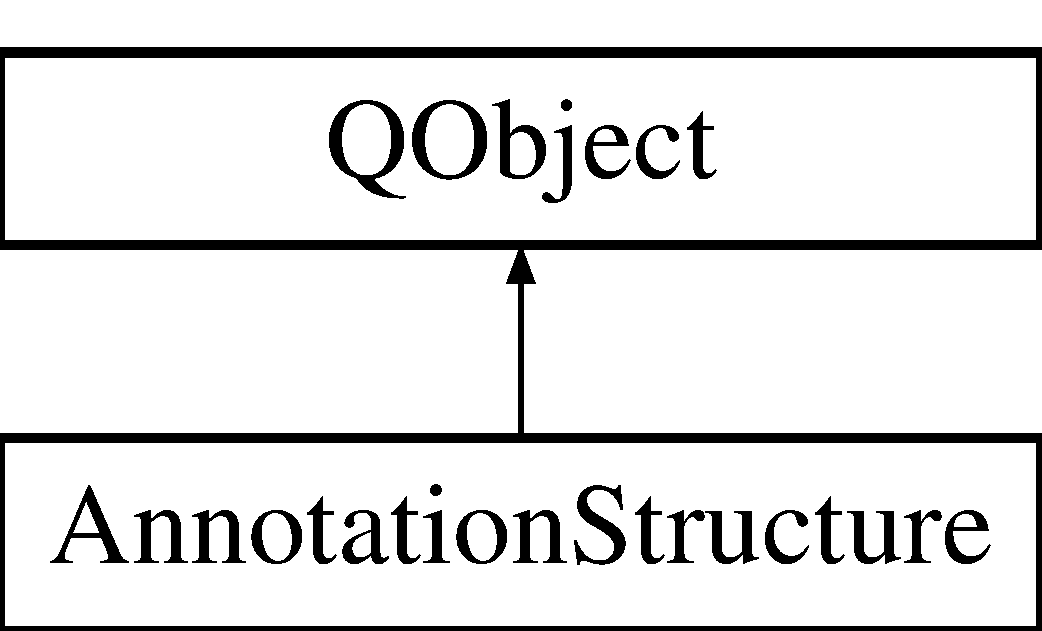
\includegraphics[height=2.000000cm]{class_annotation_structure}
\end{center}
\end{figure}
\subsection*{Signals}
\begin{DoxyCompactItemize}
\item 
\mbox{\Hypertarget{class_annotation_structure_a9839dc18e16b3a817e4cb3fffdfd351f}\label{class_annotation_structure_a9839dc18e16b3a817e4cb3fffdfd351f}} 
void {\bfseries Annotation\+Structure\+Changed} ()
\end{DoxyCompactItemize}
\subsection*{Public Member Functions}
\begin{DoxyCompactItemize}
\item 
\mbox{\Hypertarget{class_annotation_structure_a699e5000e1bebadabe29a190061cbab1}\label{class_annotation_structure_a699e5000e1bebadabe29a190061cbab1}} 
{\bfseries Annotation\+Structure} (Q\+Object $\ast$parent=nullptr)
\item 
\mbox{\Hypertarget{class_annotation_structure_adee363d0ab8c4a24faac0baae7ce1255}\label{class_annotation_structure_adee363d0ab8c4a24faac0baae7ce1255}} 
Q\+String {\bfseries ID} () const
\item 
\mbox{\Hypertarget{class_annotation_structure_aa8ca4d1a4561d59ea547e6bb0affd13e}\label{class_annotation_structure_aa8ca4d1a4561d59ea547e6bb0affd13e}} 
void {\bfseries set\+ID} (const Q\+String \&ID)
\item 
\mbox{\Hypertarget{class_annotation_structure_a01e3f5cd86558b0bee1b9ffe417179e8}\label{class_annotation_structure_a01e3f5cd86558b0bee1b9ffe417179e8}} 
void {\bfseries clear} ()
\item 
\mbox{\Hypertarget{class_annotation_structure_a73f138540af019a68e2c0f09b9b7222a}\label{class_annotation_structure_a73f138540af019a68e2c0f09b9b7222a}} 
\hyperlink{class_annotation_structure_level}{Annotation\+Structure\+Level} $\ast$ {\bfseries level} (int index) const
\item 
\mbox{\Hypertarget{class_annotation_structure_a39c00c91a24f2fd1a3ec2b431fc0e72c}\label{class_annotation_structure_a39c00c91a24f2fd1a3ec2b431fc0e72c}} 
\hyperlink{class_annotation_structure_level}{Annotation\+Structure\+Level} $\ast$ {\bfseries level} (const Q\+String \&ID) const
\item 
\mbox{\Hypertarget{class_annotation_structure_a84aad44d6c79068731a74cf9b2378297}\label{class_annotation_structure_a84aad44d6c79068731a74cf9b2378297}} 
int {\bfseries get\+Level\+Index\+By\+ID} (const Q\+String \&ID) const
\item 
\mbox{\Hypertarget{class_annotation_structure_a6d13b4ea9594708a38493f7a84378568}\label{class_annotation_structure_a6d13b4ea9594708a38493f7a84378568}} 
int {\bfseries levels\+Count} () const
\item 
\mbox{\Hypertarget{class_annotation_structure_a8cf4b14407a39d34b5b7eb790a991183}\label{class_annotation_structure_a8cf4b14407a39d34b5b7eb790a991183}} 
bool {\bfseries has\+Levels} () const
\item 
\mbox{\Hypertarget{class_annotation_structure_a65ea5f1619dec1374f304056f395b27c}\label{class_annotation_structure_a65ea5f1619dec1374f304056f395b27c}} 
bool {\bfseries has\+Level} (const Q\+String \&ID) const
\item 
\mbox{\Hypertarget{class_annotation_structure_ac38032fb6239f0c5eb5681acc1beae86}\label{class_annotation_structure_ac38032fb6239f0c5eb5681acc1beae86}} 
Q\+String\+List {\bfseries level\+I\+Ds} () const
\item 
\mbox{\Hypertarget{class_annotation_structure_a36d4b96578373292bacd3ee2ff0439a4}\label{class_annotation_structure_a36d4b96578373292bacd3ee2ff0439a4}} 
Q\+List$<$ \hyperlink{class_annotation_structure_level}{Annotation\+Structure\+Level} $\ast$ $>$ {\bfseries levels} () const
\item 
\mbox{\Hypertarget{class_annotation_structure_af7849d2348a1da8dd5cab4f3e28bb879}\label{class_annotation_structure_af7849d2348a1da8dd5cab4f3e28bb879}} 
void {\bfseries insert\+Level} (int index, \hyperlink{class_annotation_structure_level}{Annotation\+Structure\+Level} $\ast$level)
\item 
\mbox{\Hypertarget{class_annotation_structure_a7bb81c52071dd4e2f0c3dd225e428a71}\label{class_annotation_structure_a7bb81c52071dd4e2f0c3dd225e428a71}} 
void {\bfseries add\+Level} (\hyperlink{class_annotation_structure_level}{Annotation\+Structure\+Level} $\ast$level)
\item 
\mbox{\Hypertarget{class_annotation_structure_a492abcaf2c4cc847392f06b21679245f}\label{class_annotation_structure_a492abcaf2c4cc847392f06b21679245f}} 
void {\bfseries swap\+Levels} (int old\+Index, int new\+Index)
\item 
\mbox{\Hypertarget{class_annotation_structure_a54aaa46ab41650f23e07085ecf40b850}\label{class_annotation_structure_a54aaa46ab41650f23e07085ecf40b850}} 
void {\bfseries remove\+Level\+At} (int i)
\item 
\mbox{\Hypertarget{class_annotation_structure_a3d9356bad78e1cb2d2cbb6efd16b2d6b}\label{class_annotation_structure_a3d9356bad78e1cb2d2cbb6efd16b2d6b}} 
void {\bfseries remove\+Level\+By\+ID} (const Q\+String \&ID)
\end{DoxyCompactItemize}
\subsection*{Protected Attributes}
\begin{DoxyCompactItemize}
\item 
\mbox{\Hypertarget{class_annotation_structure_a6c555bdec5573e2ca3f78bb16513ab96}\label{class_annotation_structure_a6c555bdec5573e2ca3f78bb16513ab96}} 
Q\+String {\bfseries m\+\_\+\+ID}
\item 
\mbox{\Hypertarget{class_annotation_structure_a0885a62d090c26bd9f60bdb6c14f9350}\label{class_annotation_structure_a0885a62d090c26bd9f60bdb6c14f9350}} 
Q\+List$<$ \hyperlink{class_annotation_structure_level}{Annotation\+Structure\+Level} $\ast$ $>$ {\bfseries m\+\_\+levels}
\end{DoxyCompactItemize}


The documentation for this class was generated from the following files\+:\begin{DoxyCompactItemize}
\item 
/home/george/\+Develop/\+Praaline\+Py/praaline-\/core/structure/Annotation\+Structure.\+h\item 
/home/george/\+Develop/\+Praaline\+Py/praaline-\/core/structure/Annotation\+Structure.\+cpp\end{DoxyCompactItemize}

\hypertarget{class_annotation_structure_attribute}{}\section{Annotation\+Structure\+Attribute Class Reference}
\label{class_annotation_structure_attribute}\index{Annotation\+Structure\+Attribute@{Annotation\+Structure\+Attribute}}
Inheritance diagram for Annotation\+Structure\+Attribute\+:\begin{figure}[H]
\begin{center}
\leavevmode
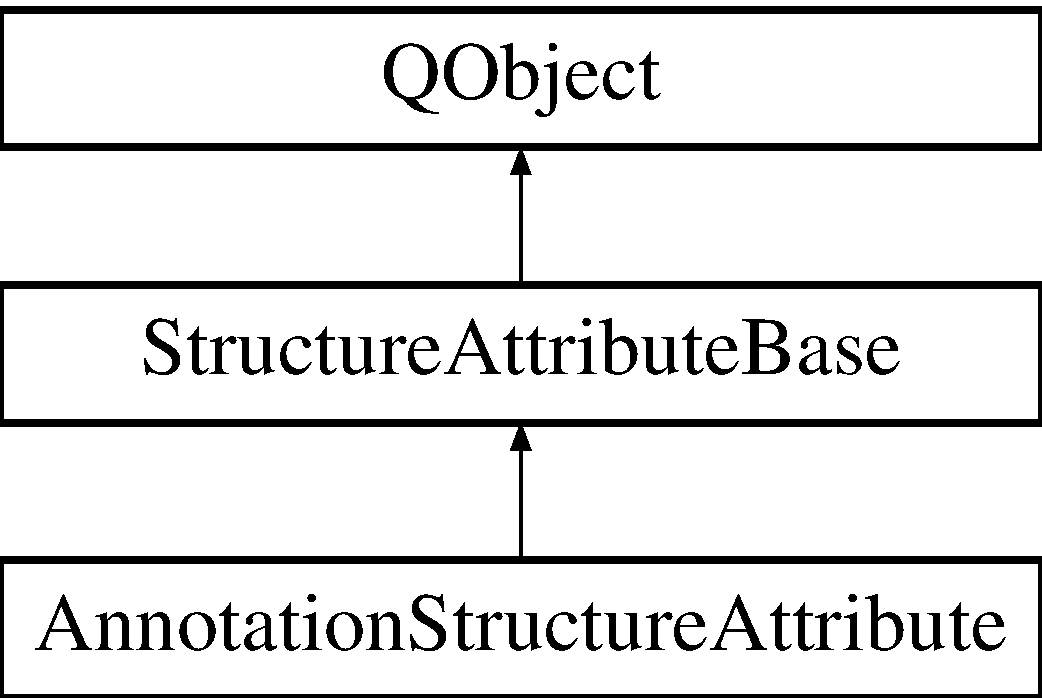
\includegraphics[height=3.000000cm]{class_annotation_structure_attribute}
\end{center}
\end{figure}
\subsection*{Public Member Functions}
\begin{DoxyCompactItemize}
\item 
\mbox{\Hypertarget{class_annotation_structure_attribute_a1c225bf9334ea55c4e483a42e918ce57}\label{class_annotation_structure_attribute_a1c225bf9334ea55c4e483a42e918ce57}} 
{\bfseries Annotation\+Structure\+Attribute} (Q\+Object $\ast$parent=nullptr)
\item 
\mbox{\Hypertarget{class_annotation_structure_attribute_a16633f3bac8c805914a5ecec94109a4f}\label{class_annotation_structure_attribute_a16633f3bac8c805914a5ecec94109a4f}} 
{\bfseries Annotation\+Structure\+Attribute} (const \hyperlink{class_annotation_structure_attribute}{Annotation\+Structure\+Attribute} $\ast$other, Q\+Object $\ast$parent=nullptr)
\item 
\mbox{\Hypertarget{class_annotation_structure_attribute_a0e8e6c7dca3c8e7377613a33dfcb3dc7}\label{class_annotation_structure_attribute_a0e8e6c7dca3c8e7377613a33dfcb3dc7}} 
{\bfseries Annotation\+Structure\+Attribute} (const Q\+String \&ID, const Q\+String \&name=Q\+String(), const Q\+String \&description=Q\+String(), const \hyperlink{class_data_type}{Data\+Type} \&datatype=\hyperlink{class_data_type}{Data\+Type}(\hyperlink{class_data_type_a8df455d8d3949b604fbb2967dfeff239a160c768176611f2649889e252c756539}{Data\+Type\+::\+Var\+Char}, 255), int order=0, bool indexed=false, const Q\+String \&name\+Value\+List=Q\+String(), Q\+Object $\ast$parent=nullptr)
\item 
\mbox{\Hypertarget{class_annotation_structure_attribute_a3783bea87144d5cbae63a1eb28c4ea94}\label{class_annotation_structure_attribute_a3783bea87144d5cbae63a1eb28c4ea94}} 
Q\+String {\bfseries stat\+Level\+Of\+Measurement} () const
\item 
\mbox{\Hypertarget{class_annotation_structure_attribute_af04deec4b660909ab6d2d22c4638c8ed}\label{class_annotation_structure_attribute_af04deec4b660909ab6d2d22c4638c8ed}} 
void {\bfseries set\+Stat\+Level\+Of\+Measurement} (const Q\+String \&stat\+Level\+Of\+Measurement)
\end{DoxyCompactItemize}
\subsection*{Protected Attributes}
\begin{DoxyCompactItemize}
\item 
\mbox{\Hypertarget{class_annotation_structure_attribute_a45098dd90f9d7638383815a7a75ed745}\label{class_annotation_structure_attribute_a45098dd90f9d7638383815a7a75ed745}} 
Q\+String {\bfseries m\+\_\+stat\+Level\+Of\+Measurement}
\end{DoxyCompactItemize}
\subsection*{Properties}
\begin{DoxyCompactItemize}
\item 
\mbox{\Hypertarget{class_annotation_structure_attribute_ac857eccd100ad3841c3d8be0000d378b}\label{class_annotation_structure_attribute_ac857eccd100ad3841c3d8be0000d378b}} 
Q\+String {\bfseries stat\+Level\+Of\+Measurement}
\end{DoxyCompactItemize}


The documentation for this class was generated from the following files\+:\begin{DoxyCompactItemize}
\item 
/home/george/\+Develop/\+Praaline\+Py/praaline-\/core/structure/Annotation\+Structure\+Attribute.\+h\item 
/home/george/\+Develop/\+Praaline\+Py/praaline-\/core/structure/Annotation\+Structure\+Attribute.\+cpp\end{DoxyCompactItemize}

\hypertarget{class_annotation_structure_level}{}\section{Annotation\+Structure\+Level Class Reference}
\label{class_annotation_structure_level}\index{Annotation\+Structure\+Level@{Annotation\+Structure\+Level}}
Inheritance diagram for Annotation\+Structure\+Level\+:\begin{figure}[H]
\begin{center}
\leavevmode
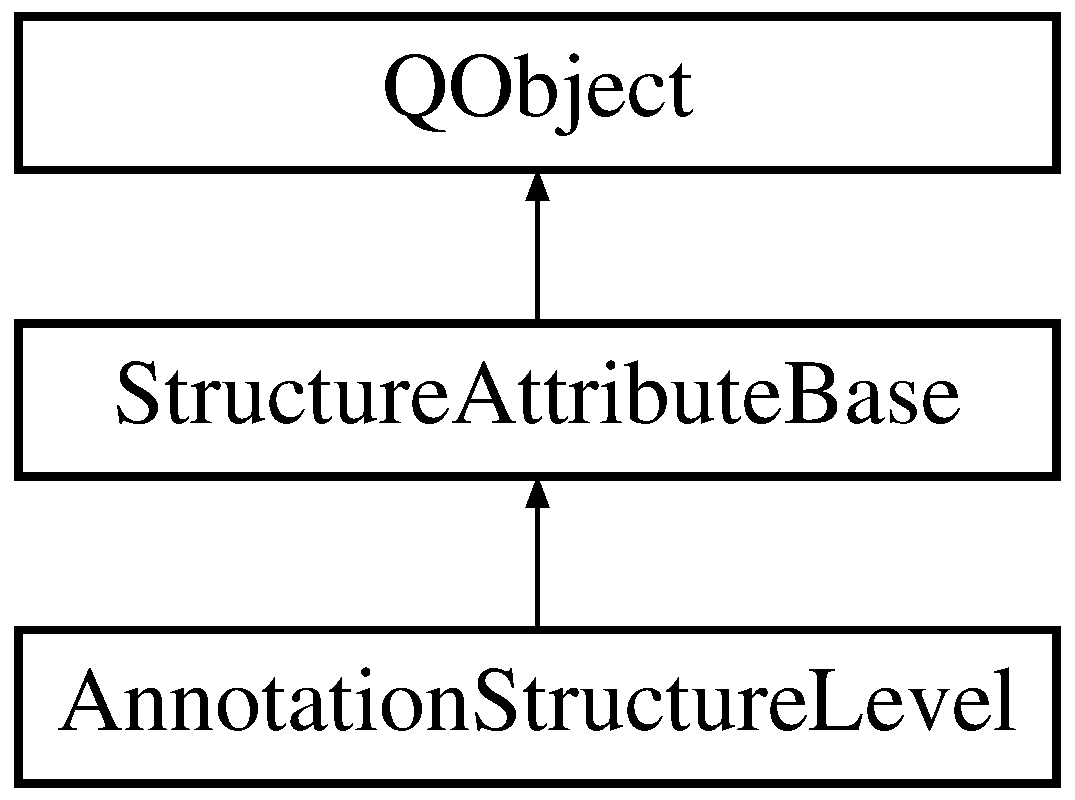
\includegraphics[height=3.000000cm]{class_annotation_structure_level}
\end{center}
\end{figure}
\subsection*{Public Types}
\begin{DoxyCompactItemize}
\item 
\mbox{\Hypertarget{class_annotation_structure_level_afc285006c7e5eb38d34b4099893cb7f5}\label{class_annotation_structure_level_afc285006c7e5eb38d34b4099893cb7f5}} 
enum {\bfseries Level\+Type} \{ \newline
{\bfseries Independent\+Points\+Level} = 10, 
{\bfseries Independent\+Intervals\+Level} = 20, 
{\bfseries Grouping\+Level} = 30, 
{\bfseries Sequences\+Level} = 40, 
\newline
{\bfseries Tree\+Level} = 50, 
{\bfseries Relations\+Level} = 60
 \}
\end{DoxyCompactItemize}
\subsection*{Public Member Functions}
\begin{DoxyCompactItemize}
\item 
\mbox{\Hypertarget{class_annotation_structure_level_a3d27dbadf04532e73024a2c9cd94a2da}\label{class_annotation_structure_level_a3d27dbadf04532e73024a2c9cd94a2da}} 
{\bfseries Annotation\+Structure\+Level} (Q\+Object $\ast$parent=nullptr)
\item 
\mbox{\Hypertarget{class_annotation_structure_level_ab85043cd1f2e34a92fa205b97ef58ad5}\label{class_annotation_structure_level_ab85043cd1f2e34a92fa205b97ef58ad5}} 
{\bfseries Annotation\+Structure\+Level} (const Q\+String \&ID, Level\+Type type=Independent\+Intervals\+Level, const Q\+String \&name=Q\+String(), const Q\+String \&description=Q\+String(), const Q\+String \&parent\+Level\+ID=Q\+String(), const \hyperlink{class_data_type}{Data\+Type} \&datatype=\hyperlink{class_data_type}{Data\+Type}(\hyperlink{class_data_type_a8df455d8d3949b604fbb2967dfeff239a160c768176611f2649889e252c756539}{Data\+Type\+::\+Var\+Char}, 1024), int order=0, bool indexed=false, const Q\+String \&name\+Value\+List=Q\+String(), Q\+Object $\ast$parent=nullptr)
\item 
\mbox{\Hypertarget{class_annotation_structure_level_aa69940d5dd044fed5a848788633e3573}\label{class_annotation_structure_level_aa69940d5dd044fed5a848788633e3573}} 
Level\+Type {\bfseries level\+Type} () const
\item 
\mbox{\Hypertarget{class_annotation_structure_level_acdac30a3532497e2995c4f7d0055476c}\label{class_annotation_structure_level_acdac30a3532497e2995c4f7d0055476c}} 
bool {\bfseries is\+Level\+Type\+Primary} () const
\item 
\mbox{\Hypertarget{class_annotation_structure_level_aee293305035809bcd57a3476912f7784}\label{class_annotation_structure_level_aee293305035809bcd57a3476912f7784}} 
void {\bfseries set\+Level\+Type} (Level\+Type type)
\item 
\mbox{\Hypertarget{class_annotation_structure_level_a56eb69db99dbafbe878a84a59a97645b}\label{class_annotation_structure_level_a56eb69db99dbafbe878a84a59a97645b}} 
Q\+String {\bfseries parent\+Level\+ID} () const
\item 
\mbox{\Hypertarget{class_annotation_structure_level_ae076985df9a024cab28a357d96ddbeed}\label{class_annotation_structure_level_ae076985df9a024cab28a357d96ddbeed}} 
void {\bfseries set\+Parent\+Level\+ID} (const Q\+String \&parent\+Level\+ID)
\item 
\mbox{\Hypertarget{class_annotation_structure_level_aaa843ffde9f31c28052263fb6ef4f9e0}\label{class_annotation_structure_level_aaa843ffde9f31c28052263fb6ef4f9e0}} 
Q\+Pointer$<$ \hyperlink{class_annotation_structure_attribute}{Annotation\+Structure\+Attribute} $>$ {\bfseries attribute} (int index) const
\item 
\mbox{\Hypertarget{class_annotation_structure_level_a096ca66fca9d2226bbbb7558518587d1}\label{class_annotation_structure_level_a096ca66fca9d2226bbbb7558518587d1}} 
Q\+Pointer$<$ \hyperlink{class_annotation_structure_attribute}{Annotation\+Structure\+Attribute} $>$ {\bfseries attribute} (const Q\+String \&ID) const
\item 
\mbox{\Hypertarget{class_annotation_structure_level_af679873831d05ade95e7d7587b5e1dcc}\label{class_annotation_structure_level_af679873831d05ade95e7d7587b5e1dcc}} 
int {\bfseries attribute\+Index\+By\+ID} (const Q\+String \&ID) const
\item 
\mbox{\Hypertarget{class_annotation_structure_level_a726491c28b63f3140c9c1e2f6e6c0c2a}\label{class_annotation_structure_level_a726491c28b63f3140c9c1e2f6e6c0c2a}} 
int {\bfseries attributes\+Count} () const
\item 
\mbox{\Hypertarget{class_annotation_structure_level_af1b1599c8048b257293c34c8390658d5}\label{class_annotation_structure_level_af1b1599c8048b257293c34c8390658d5}} 
bool {\bfseries has\+Attributes} () const
\item 
\mbox{\Hypertarget{class_annotation_structure_level_a041f830775922af4ea907d070a039080}\label{class_annotation_structure_level_a041f830775922af4ea907d070a039080}} 
bool {\bfseries has\+Attribute} (const Q\+String \&ID)
\item 
\mbox{\Hypertarget{class_annotation_structure_level_ada820074c9207c1601100c92f5d9796b}\label{class_annotation_structure_level_ada820074c9207c1601100c92f5d9796b}} 
Q\+String\+List {\bfseries attribute\+I\+Ds} () const
\item 
\mbox{\Hypertarget{class_annotation_structure_level_af893384c9a873ce8816505364358dfb4}\label{class_annotation_structure_level_af893384c9a873ce8816505364358dfb4}} 
Q\+List$<$ Q\+Pointer$<$ \hyperlink{class_annotation_structure_attribute}{Annotation\+Structure\+Attribute} $>$ $>$ {\bfseries attributes} () const
\item 
\mbox{\Hypertarget{class_annotation_structure_level_aa77cfa1015672e248eed37ea75db7e47}\label{class_annotation_structure_level_aa77cfa1015672e248eed37ea75db7e47}} 
void {\bfseries insert\+Attribute} (int index, \hyperlink{class_annotation_structure_attribute}{Annotation\+Structure\+Attribute} $\ast$attribute)
\item 
\mbox{\Hypertarget{class_annotation_structure_level_adbf3154e9893a0ea975751638b277bf2}\label{class_annotation_structure_level_adbf3154e9893a0ea975751638b277bf2}} 
void {\bfseries add\+Attribute} (\hyperlink{class_annotation_structure_attribute}{Annotation\+Structure\+Attribute} $\ast$attribute)
\item 
\mbox{\Hypertarget{class_annotation_structure_level_af9d0d8200d766bd166051feaad209e8a}\label{class_annotation_structure_level_af9d0d8200d766bd166051feaad209e8a}} 
void {\bfseries swap\+Attribute} (int old\+Index, int new\+Index)
\item 
\mbox{\Hypertarget{class_annotation_structure_level_a7640b925290bd80f46aa0931043abb1b}\label{class_annotation_structure_level_a7640b925290bd80f46aa0931043abb1b}} 
void {\bfseries remove\+Attribute\+At} (int i)
\item 
\mbox{\Hypertarget{class_annotation_structure_level_a8d8865e606c5ee399d7b0e3e904f0e19}\label{class_annotation_structure_level_a8d8865e606c5ee399d7b0e3e904f0e19}} 
void {\bfseries remove\+Attribute\+By\+ID} (const Q\+String \&ID)
\end{DoxyCompactItemize}
\subsection*{Protected Attributes}
\begin{DoxyCompactItemize}
\item 
\mbox{\Hypertarget{class_annotation_structure_level_a76285d7e363afd93464bd7ef7ed048ec}\label{class_annotation_structure_level_a76285d7e363afd93464bd7ef7ed048ec}} 
Level\+Type {\bfseries m\+\_\+level\+Type}
\item 
\mbox{\Hypertarget{class_annotation_structure_level_a6a5eee5ebd6f8e266be3ac2fa09f6ccc}\label{class_annotation_structure_level_a6a5eee5ebd6f8e266be3ac2fa09f6ccc}} 
Q\+String {\bfseries m\+\_\+parent\+Level\+ID}
\item 
\mbox{\Hypertarget{class_annotation_structure_level_a74c9169103a7c2d818feb6465156786e}\label{class_annotation_structure_level_a74c9169103a7c2d818feb6465156786e}} 
Q\+List$<$ Q\+Pointer$<$ \hyperlink{class_annotation_structure_attribute}{Annotation\+Structure\+Attribute} $>$ $>$ {\bfseries m\+\_\+attributes}
\end{DoxyCompactItemize}
\subsection*{Properties}
\begin{DoxyCompactItemize}
\item 
\mbox{\Hypertarget{class_annotation_structure_level_ac4e448ffc536acb2c7c43c5988aeb925}\label{class_annotation_structure_level_ac4e448ffc536acb2c7c43c5988aeb925}} 
Level\+Type {\bfseries level\+Type}
\item 
\mbox{\Hypertarget{class_annotation_structure_level_a2dfe6d8522dcfa8d86d9177ae8b282af}\label{class_annotation_structure_level_a2dfe6d8522dcfa8d86d9177ae8b282af}} 
Q\+String {\bfseries parent\+Level\+ID}
\end{DoxyCompactItemize}


The documentation for this class was generated from the following files\+:\begin{DoxyCompactItemize}
\item 
/home/george/\+Develop/\+Praaline\+Py/praaline-\/core/structure/Annotation\+Structure\+Level.\+h\item 
/home/george/\+Develop/\+Praaline\+Py/praaline-\/core/structure/Annotation\+Structure\+Level.\+cpp\end{DoxyCompactItemize}

\hypertarget{class_annotation_tier}{}\section{Annotation\+Tier Class Reference}
\label{class_annotation_tier}\index{Annotation\+Tier@{Annotation\+Tier}}
Inheritance diagram for Annotation\+Tier\+:\begin{figure}[H]
\begin{center}
\leavevmode
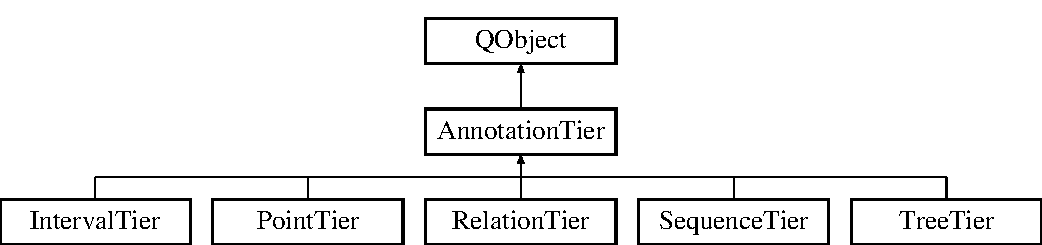
\includegraphics[height=3.000000cm]{class_annotation_tier}
\end{center}
\end{figure}
\subsection*{Public Types}
\begin{DoxyCompactItemize}
\item 
\mbox{\Hypertarget{class_annotation_tier_aad0b7862687212adcd3b2851fd62ba5d}\label{class_annotation_tier_aad0b7862687212adcd3b2851fd62ba5d}} 
enum {\bfseries Tier\+Type} \{ \newline
{\bfseries Tier\+Type\+\_\+\+Points}, 
{\bfseries Tier\+Type\+\_\+\+Intervals}, 
{\bfseries Tier\+Type\+\_\+\+Grouping}, 
{\bfseries Tier\+Type\+\_\+\+Sequences}, 
\newline
{\bfseries Tier\+Type\+\_\+\+Tree}, 
{\bfseries Tier\+Type\+\_\+\+Relations}
 \}
\end{DoxyCompactItemize}
\subsection*{Signals}
\begin{DoxyCompactItemize}
\item 
\mbox{\Hypertarget{class_annotation_tier_a26b44c87723f7e537a952a3342dfa784}\label{class_annotation_tier_a26b44c87723f7e537a952a3342dfa784}} 
void {\bfseries name\+Changed} ()
\end{DoxyCompactItemize}
\subsection*{Public Member Functions}
\begin{DoxyCompactItemize}
\item 
\mbox{\Hypertarget{class_annotation_tier_af59a01566de15fb6f767d14da6e34a94}\label{class_annotation_tier_af59a01566de15fb6f767d14da6e34a94}} 
{\bfseries Annotation\+Tier} (const Q\+String \&name=Q\+String(), Q\+Object $\ast$parent=nullptr)
\item 
\mbox{\Hypertarget{class_annotation_tier_abde1704c32f26e05f946c4eb79cf2948}\label{class_annotation_tier_abde1704c32f26e05f946c4eb79cf2948}} 
virtual Tier\+Type {\bfseries tier\+Type} () const =0
\item 
\mbox{\Hypertarget{class_annotation_tier_a6588948ba81099274eb55e8813fbbd88}\label{class_annotation_tier_a6588948ba81099274eb55e8813fbbd88}} 
virtual Q\+String {\bfseries name} () const
\item 
\mbox{\Hypertarget{class_annotation_tier_ada164999ed11f552b9ed196743f30c43}\label{class_annotation_tier_ada164999ed11f552b9ed196743f30c43}} 
virtual void {\bfseries set\+Name} (const Q\+String \&name)
\item 
\mbox{\Hypertarget{class_annotation_tier_afaf3e5815e8c21678abaf1766a317de4}\label{class_annotation_tier_afaf3e5815e8c21678abaf1766a317de4}} 
virtual \hyperlink{struct_real_time}{Real\+Time} {\bfseries t\+Min} () const
\item 
\mbox{\Hypertarget{class_annotation_tier_a4df732bb51ad92f493900e0d1d822dcf}\label{class_annotation_tier_a4df732bb51ad92f493900e0d1d822dcf}} 
virtual \hyperlink{struct_real_time}{Real\+Time} {\bfseries t\+Max} () const
\item 
\mbox{\Hypertarget{class_annotation_tier_a2afaa711c02f66e632f9841218836233}\label{class_annotation_tier_a2afaa711c02f66e632f9841218836233}} 
virtual \hyperlink{struct_real_time}{Real\+Time} {\bfseries duration} () const
\item 
\mbox{\Hypertarget{class_annotation_tier_a53d2439519ccda4962ba2c35c76cab53}\label{class_annotation_tier_a53d2439519ccda4962ba2c35c76cab53}} 
virtual int {\bfseries count} () const =0
\item 
\mbox{\Hypertarget{class_annotation_tier_a0f545d0930ead88cb4e9fb01a5ed5097}\label{class_annotation_tier_a0f545d0930ead88cb4e9fb01a5ed5097}} 
virtual bool {\bfseries is\+Empty} () const =0
\item 
\mbox{\Hypertarget{class_annotation_tier_ae83ced90eff441f3392837b310cfa07d}\label{class_annotation_tier_ae83ced90eff441f3392837b310cfa07d}} 
virtual void {\bfseries clear} ()=0
\item 
\mbox{\Hypertarget{class_annotation_tier_ae8c2d7407cb31ec6917aa2e2c711a58c}\label{class_annotation_tier_ae8c2d7407cb31ec6917aa2e2c711a58c}} 
virtual \hyperlink{class_annotation_element}{Annotation\+Element} $\ast$ {\bfseries at} (int index) const =0
\item 
\mbox{\Hypertarget{class_annotation_tier_a7501382f881d2956ad172e25a13f4c71}\label{class_annotation_tier_a7501382f881d2956ad172e25a13f4c71}} 
virtual \hyperlink{class_annotation_element}{Annotation\+Element} $\ast$ {\bfseries first} () const =0
\item 
\mbox{\Hypertarget{class_annotation_tier_aee3de82bbe9757962887068e5e2e10dd}\label{class_annotation_tier_aee3de82bbe9757962887068e5e2e10dd}} 
virtual \hyperlink{class_annotation_element}{Annotation\+Element} $\ast$ {\bfseries last} () const =0
\item 
\mbox{\Hypertarget{class_annotation_tier_a057f6668e07be7e6230955b2c241df1c}\label{class_annotation_tier_a057f6668e07be7e6230955b2c241df1c}} 
virtual Q\+String\+List {\bfseries get\+Distinct\+Labels} () const =0
\item 
\mbox{\Hypertarget{class_annotation_tier_a1f03d603d941c958c4cf5d0f809305b4}\label{class_annotation_tier_a1f03d603d941c958c4cf5d0f809305b4}} 
virtual Q\+List$<$ Q\+Variant $>$ {\bfseries get\+Distinct\+Values} (const Q\+String \&attribute\+ID) const =0
\item 
\mbox{\Hypertarget{class_annotation_tier_a97599d1c53b5ce0b73d5a96cf4fbe872}\label{class_annotation_tier_a97599d1c53b5ce0b73d5a96cf4fbe872}} 
virtual void {\bfseries replace} (const Q\+String \&attribute\+ID, const Q\+String \&before, const Q\+String \&after, Qt\+::\+Case\+Sensitivity cs=Qt\+::\+Case\+Sensitive)=0
\item 
\mbox{\Hypertarget{class_annotation_tier_aa0c5186b64e95e2c54070f9e7dc73cae}\label{class_annotation_tier_aa0c5186b64e95e2c54070f9e7dc73cae}} 
virtual void {\bfseries fill\+Empty\+With} (const Q\+String \&attribute\+ID, const Q\+String \&filler)=0
\end{DoxyCompactItemize}
\subsection*{Protected Attributes}
\begin{DoxyCompactItemize}
\item 
\mbox{\Hypertarget{class_annotation_tier_a24cca2a0647ac26993600fc1340f542d}\label{class_annotation_tier_a24cca2a0647ac26993600fc1340f542d}} 
Q\+String {\bfseries m\+\_\+name}
\item 
\mbox{\Hypertarget{class_annotation_tier_afcca9fbd63e626e84490f7c95d71e09b}\label{class_annotation_tier_afcca9fbd63e626e84490f7c95d71e09b}} 
\hyperlink{struct_real_time}{Real\+Time} {\bfseries m\+\_\+t\+Min}
\item 
\mbox{\Hypertarget{class_annotation_tier_a05d59926099e9a3d45d18a84934b745c}\label{class_annotation_tier_a05d59926099e9a3d45d18a84934b745c}} 
\hyperlink{struct_real_time}{Real\+Time} {\bfseries m\+\_\+t\+Max}
\end{DoxyCompactItemize}
\subsection*{Properties}
\begin{DoxyCompactItemize}
\item 
\mbox{\Hypertarget{class_annotation_tier_a421ef99d21e002f1a5724c25ca016aa4}\label{class_annotation_tier_a421ef99d21e002f1a5724c25ca016aa4}} 
Q\+String {\bfseries name}
\item 
\mbox{\Hypertarget{class_annotation_tier_a20b9f0514d945098b014dafe7217cece}\label{class_annotation_tier_a20b9f0514d945098b014dafe7217cece}} 
\hyperlink{struct_real_time}{Real\+Time} {\bfseries t\+Min}
\item 
\mbox{\Hypertarget{class_annotation_tier_a719a756eb98dfebebc0fb5fae78e45b6}\label{class_annotation_tier_a719a756eb98dfebebc0fb5fae78e45b6}} 
\hyperlink{struct_real_time}{Real\+Time} {\bfseries t\+Max}
\item 
\mbox{\Hypertarget{class_annotation_tier_a67d00a5e50a49acc3dc43bb1d3652c7a}\label{class_annotation_tier_a67d00a5e50a49acc3dc43bb1d3652c7a}} 
\hyperlink{struct_real_time}{Real\+Time} {\bfseries duration}
\end{DoxyCompactItemize}


The documentation for this class was generated from the following files\+:\begin{DoxyCompactItemize}
\item 
/home/george/\+Develop/\+Praaline\+Py/praaline-\/core/annotation/Annotation\+Tier.\+h\item 
/home/george/\+Develop/\+Praaline\+Py/praaline-\/core/annotation/Annotation\+Tier.\+cpp\end{DoxyCompactItemize}

\hypertarget{class_annotation_tier_group}{}\section{Annotation\+Tier\+Group Class Reference}
\label{class_annotation_tier_group}\index{Annotation\+Tier\+Group@{Annotation\+Tier\+Group}}
Inheritance diagram for Annotation\+Tier\+Group\+:\begin{figure}[H]
\begin{center}
\leavevmode
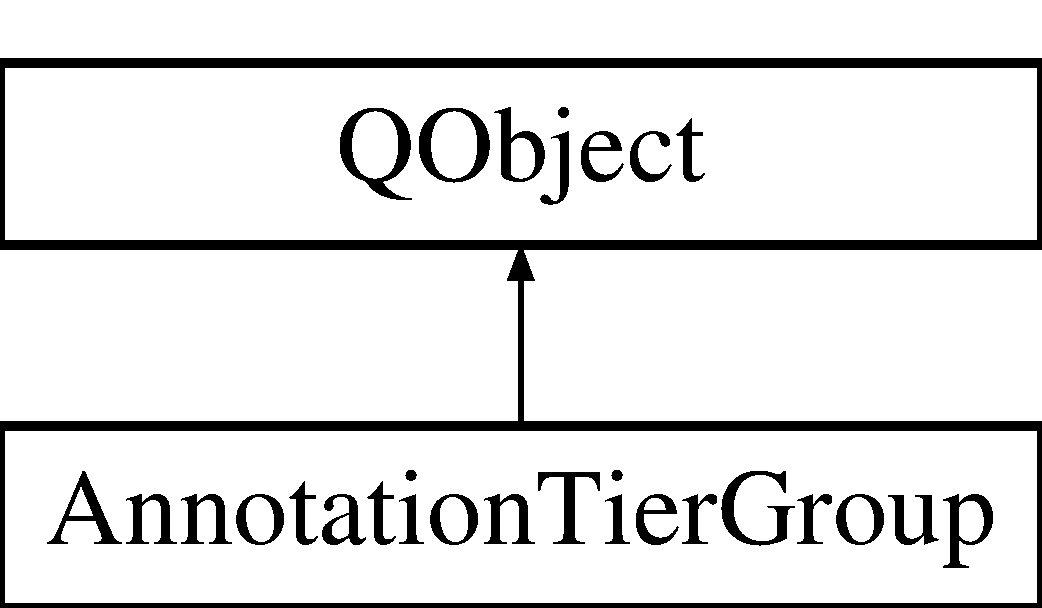
\includegraphics[height=2.000000cm]{class_annotation_tier_group}
\end{center}
\end{figure}
\subsection*{Signals}
\begin{DoxyCompactItemize}
\item 
\mbox{\Hypertarget{class_annotation_tier_group_a13088d0f3786f1d1b171d99623856efc}\label{class_annotation_tier_group_a13088d0f3786f1d1b171d99623856efc}} 
void {\bfseries tier\+Inserted} (\hyperlink{class_annotation_tier}{Annotation\+Tier} $\ast$tier)
\item 
\mbox{\Hypertarget{class_annotation_tier_group_af567945dc914d185458e5e5b33ac2351}\label{class_annotation_tier_group_af567945dc914d185458e5e5b33ac2351}} 
void {\bfseries tier\+Deleted} (Q\+String tier\+Name)
\end{DoxyCompactItemize}
\subsection*{Public Member Functions}
\begin{DoxyCompactItemize}
\item 
\mbox{\Hypertarget{class_annotation_tier_group_a1f9216569e4472d42a03d56d1d8d85ab}\label{class_annotation_tier_group_a1f9216569e4472d42a03d56d1d8d85ab}} 
{\bfseries Annotation\+Tier\+Group} (Q\+Object $\ast$parent=nullptr)
\item 
\mbox{\Hypertarget{class_annotation_tier_group_ab15b7541e671ee5b689d2b0439c34813}\label{class_annotation_tier_group_ab15b7541e671ee5b689d2b0439c34813}} 
Q\+String {\bfseries ID} () const
\item 
\mbox{\Hypertarget{class_annotation_tier_group_af35d66ef4ee1f95f8717f6d092b16450}\label{class_annotation_tier_group_af35d66ef4ee1f95f8717f6d092b16450}} 
void {\bfseries set\+ID} (const Q\+String \&ID)
\item 
\mbox{\Hypertarget{class_annotation_tier_group_a0ddaad6d5fc3842284eef55e44a3f278}\label{class_annotation_tier_group_a0ddaad6d5fc3842284eef55e44a3f278}} 
\hyperlink{struct_real_time}{Real\+Time} {\bfseries t\+Min} () const
\item 
\mbox{\Hypertarget{class_annotation_tier_group_ac3c30ab4c2b06825b50e97f14138db8c}\label{class_annotation_tier_group_ac3c30ab4c2b06825b50e97f14138db8c}} 
\hyperlink{struct_real_time}{Real\+Time} {\bfseries t\+Max} () const
\item 
\mbox{\Hypertarget{class_annotation_tier_group_a88a5b0eda8ff9043c45ad27b0e10f848}\label{class_annotation_tier_group_a88a5b0eda8ff9043c45ad27b0e10f848}} 
\hyperlink{struct_real_time}{Real\+Time} {\bfseries duration} () const
\item 
\mbox{\Hypertarget{class_annotation_tier_group_a7ecc7a86af2df4a514718680eac1630d}\label{class_annotation_tier_group_a7ecc7a86af2df4a514718680eac1630d}} 
\hyperlink{class_annotation_tier}{Annotation\+Tier} $\ast$ {\bfseries tier} (int index) const
\item 
\mbox{\Hypertarget{class_annotation_tier_group_a61f8204c07bb2b214ad5f3858b974bba}\label{class_annotation_tier_group_a61f8204c07bb2b214ad5f3858b974bba}} 
\hyperlink{class_annotation_tier}{Annotation\+Tier} $\ast$ {\bfseries tier} (const Q\+String \&name) const
\item 
\mbox{\Hypertarget{class_annotation_tier_group_a84bd7ee636bc58b353f8557f89910a43}\label{class_annotation_tier_group_a84bd7ee636bc58b353f8557f89910a43}} 
int {\bfseries tiers\+Count} () const
\item 
\mbox{\Hypertarget{class_annotation_tier_group_a3a9e5dfe0b01d4acfd8e28289c9d75ee}\label{class_annotation_tier_group_a3a9e5dfe0b01d4acfd8e28289c9d75ee}} 
bool {\bfseries has\+Tiers} () const
\item 
\mbox{\Hypertarget{class_annotation_tier_group_a0a868f1406c1c5b989b9303bb1000715}\label{class_annotation_tier_group_a0a868f1406c1c5b989b9303bb1000715}} 
Q\+List$<$ \hyperlink{class_annotation_tier}{Annotation\+Tier} $\ast$ $>$ {\bfseries tiers} () const
\item 
\mbox{\Hypertarget{class_annotation_tier_group_a9f6129cfdb96ce9084d49f4a4f3f9581}\label{class_annotation_tier_group_a9f6129cfdb96ce9084d49f4a4f3f9581}} 
void {\bfseries insert\+Tier} (int index, \hyperlink{class_annotation_tier}{Annotation\+Tier} $\ast$tier)
\item 
\mbox{\Hypertarget{class_annotation_tier_group_a394c786058d3650fb2b170493ad21454}\label{class_annotation_tier_group_a394c786058d3650fb2b170493ad21454}} 
void {\bfseries insert\+Tier\+Replacing} (int index, \hyperlink{class_annotation_tier}{Annotation\+Tier} $\ast$tier)
\item 
\mbox{\Hypertarget{class_annotation_tier_group_a96df167d0aac7e8f38cd8267a29d5f33}\label{class_annotation_tier_group_a96df167d0aac7e8f38cd8267a29d5f33}} 
void {\bfseries add\+Tier} (\hyperlink{class_annotation_tier}{Annotation\+Tier} $\ast$tier)
\item 
\mbox{\Hypertarget{class_annotation_tier_group_ad477a0009c24b987406dbf1dc3d4d9a0}\label{class_annotation_tier_group_ad477a0009c24b987406dbf1dc3d4d9a0}} 
void {\bfseries add\+Tier\+Replacing} (\hyperlink{class_annotation_tier}{Annotation\+Tier} $\ast$tier)
\item 
\mbox{\Hypertarget{class_annotation_tier_group_ad7fb9197ffbf6d128ce0d0e8c9c42874}\label{class_annotation_tier_group_ad7fb9197ffbf6d128ce0d0e8c9c42874}} 
void {\bfseries swap\+Tiers} (int old\+Index, int new\+Index)
\item 
\mbox{\Hypertarget{class_annotation_tier_group_aeded4a0c4c3d6a7f2f5df08b042c3349}\label{class_annotation_tier_group_aeded4a0c4c3d6a7f2f5df08b042c3349}} 
void {\bfseries remove\+Tier\+At} (int i)
\item 
\mbox{\Hypertarget{class_annotation_tier_group_a77b0a3cce3e181340446c1ed53fee04b}\label{class_annotation_tier_group_a77b0a3cce3e181340446c1ed53fee04b}} 
void {\bfseries remove\+Tier\+By\+Name} (const Q\+String \&name)
\item 
\mbox{\Hypertarget{class_annotation_tier_group_a298ac8f51f3ed8ef502c64c0f707751f}\label{class_annotation_tier_group_a298ac8f51f3ed8ef502c64c0f707751f}} 
void {\bfseries rename\+Tier} (const Q\+String \&name\+Before, const Q\+String \&name\+After)
\item 
\mbox{\Hypertarget{class_annotation_tier_group_ad375da2b5d84a63fbf6255c5813a579e}\label{class_annotation_tier_group_ad375da2b5d84a63fbf6255c5813a579e}} 
\hyperlink{class_interval_tier}{Interval\+Tier} $\ast$ {\bfseries get\+Interval\+Tier\+By\+Name} (const Q\+String \&name) const
\item 
\mbox{\Hypertarget{class_annotation_tier_group_a75c8efe087b3158f9c7769a1d1e720de}\label{class_annotation_tier_group_a75c8efe087b3158f9c7769a1d1e720de}} 
\hyperlink{class_interval_tier}{Interval\+Tier} $\ast$ {\bfseries get\+Interval\+Tier\+By\+Index} (int index) const
\item 
\mbox{\Hypertarget{class_annotation_tier_group_a77efe7e0e65f895bf2c3d6d5dc5afe41}\label{class_annotation_tier_group_a77efe7e0e65f895bf2c3d6d5dc5afe41}} 
\hyperlink{class_point_tier}{Point\+Tier} $\ast$ {\bfseries get\+Point\+Tier\+By\+Name} (const Q\+String \&name) const
\item 
\mbox{\Hypertarget{class_annotation_tier_group_a1b381a663af16fd87582b7645e6a3b0a}\label{class_annotation_tier_group_a1b381a663af16fd87582b7645e6a3b0a}} 
\hyperlink{class_point_tier}{Point\+Tier} $\ast$ {\bfseries get\+Point\+Tier\+By\+Index} (int index) const
\item 
\mbox{\Hypertarget{class_annotation_tier_group_a5a666bcf4b60f4ea42bfc56e6970207c}\label{class_annotation_tier_group_a5a666bcf4b60f4ea42bfc56e6970207c}} 
\hyperlink{class_sequence_tier}{Sequence\+Tier} $\ast$ {\bfseries get\+Sequence\+Tier\+By\+Name} (const Q\+String \&name) const
\item 
\mbox{\Hypertarget{class_annotation_tier_group_a71049bb192a09d3dc4cc0d7eddb7d157}\label{class_annotation_tier_group_a71049bb192a09d3dc4cc0d7eddb7d157}} 
\hyperlink{class_sequence_tier}{Sequence\+Tier} $\ast$ {\bfseries get\+Sequence\+Tier\+By\+Index} (int index) const
\item 
\mbox{\Hypertarget{class_annotation_tier_group_a263bcfc93cd75b6818f54089c7c8d6ac}\label{class_annotation_tier_group_a263bcfc93cd75b6818f54089c7c8d6ac}} 
\hyperlink{class_tree_tier}{Tree\+Tier} $\ast$ {\bfseries get\+Tree\+Tier\+By\+Name} (const Q\+String \&name) const
\item 
\mbox{\Hypertarget{class_annotation_tier_group_a48c30da8b1807b0fd46fd7da343a7234}\label{class_annotation_tier_group_a48c30da8b1807b0fd46fd7da343a7234}} 
\hyperlink{class_tree_tier}{Tree\+Tier} $\ast$ {\bfseries get\+Tree\+Tier\+By\+Index} (int index) const
\item 
\mbox{\Hypertarget{class_annotation_tier_group_a2d8fe2a9050f5aca66bd61ae797f19cb}\label{class_annotation_tier_group_a2d8fe2a9050f5aca66bd61ae797f19cb}} 
\hyperlink{class_relation_tier}{Relation\+Tier} $\ast$ {\bfseries get\+Relation\+Tier\+By\+Name} (const Q\+String \&name) const
\item 
\mbox{\Hypertarget{class_annotation_tier_group_a187b9cfbeb741c78c8469fa300dee887}\label{class_annotation_tier_group_a187b9cfbeb741c78c8469fa300dee887}} 
\hyperlink{class_relation_tier}{Relation\+Tier} $\ast$ {\bfseries get\+Relation\+Tier\+By\+Index} (int index) const
\item 
\mbox{\Hypertarget{class_annotation_tier_group_ad2c96e89f53ccfab2f667727bc995ec7}\label{class_annotation_tier_group_ad2c96e89f53ccfab2f667727bc995ec7}} 
int {\bfseries get\+Tier\+Index\+By\+Name} (const Q\+String \&name) const
\item 
\mbox{\Hypertarget{class_annotation_tier_group_a9eaf011f0a807f95db993bfe826cffc7}\label{class_annotation_tier_group_a9eaf011f0a807f95db993bfe826cffc7}} 
Q\+String\+List {\bfseries tier\+Names} () const
\item 
\mbox{\Hypertarget{class_annotation_tier_group_a1a45061aa5edd02b0fe4fcf832c63911}\label{class_annotation_tier_group_a1a45061aa5edd02b0fe4fcf832c63911}} 
void {\bfseries insert\+Tier\+Clone} (int index, const \hyperlink{class_annotation_tier}{Annotation\+Tier} $\ast$tier, const Q\+String \&new\+Name)
\item 
\mbox{\Hypertarget{class_annotation_tier_group_a798aa6ba5d352ec09693ced0fe6773d4}\label{class_annotation_tier_group_a798aa6ba5d352ec09693ced0fe6773d4}} 
bool {\bfseries reorder\+Tiers} (Q\+String\+List tier\+Names\+In\+New\+Order)
\item 
\mbox{\Hypertarget{class_annotation_tier_group_a2ed5a9803b673f8fdf76de842a45f599}\label{class_annotation_tier_group_a2ed5a9803b673f8fdf76de842a45f599}} 
void {\bfseries merge\+Silent\+Pauses\+On\+All\+Interval\+Tiers} (const Q\+String \&silent\+Pause\+Text)
\end{DoxyCompactItemize}
\subsection*{Protected Attributes}
\begin{DoxyCompactItemize}
\item 
\mbox{\Hypertarget{class_annotation_tier_group_a4b219b439c4d301bcc6ed814bd7cb868}\label{class_annotation_tier_group_a4b219b439c4d301bcc6ed814bd7cb868}} 
Q\+String {\bfseries m\+\_\+\+ID}
\item 
\mbox{\Hypertarget{class_annotation_tier_group_a73d9af796b7cd6c75dc563b702083a50}\label{class_annotation_tier_group_a73d9af796b7cd6c75dc563b702083a50}} 
Q\+List$<$ \hyperlink{class_annotation_tier}{Annotation\+Tier} $\ast$ $>$ {\bfseries m\+\_\+tiers}
\item 
\mbox{\Hypertarget{class_annotation_tier_group_a8391f2110068e88fbcbfd9da0aa02c67}\label{class_annotation_tier_group_a8391f2110068e88fbcbfd9da0aa02c67}} 
Q\+String {\bfseries annotation\+ID}
\item 
\mbox{\Hypertarget{class_annotation_tier_group_a0a25c4f69d95d5a05c4a36b2ce27cf22}\label{class_annotation_tier_group_a0a25c4f69d95d5a05c4a36b2ce27cf22}} 
Q\+String {\bfseries speaker\+ID}
\end{DoxyCompactItemize}


The documentation for this class was generated from the following files\+:\begin{DoxyCompactItemize}
\item 
/home/george/\+Develop/\+Praaline\+Py/praaline-\/core/annotation/Annotation\+Tier\+Group.\+h\item 
/home/george/\+Develop/\+Praaline\+Py/praaline-\/core/annotation/Annotation\+Tier\+Group.\+cpp\end{DoxyCompactItemize}

\hypertarget{class_anvil_metadata_transcript}{}\section{Anvil\+Metadata\+Transcript Class Reference}
\label{class_anvil_metadata_transcript}\index{Anvil\+Metadata\+Transcript@{Anvil\+Metadata\+Transcript}}
Inheritance diagram for Anvil\+Metadata\+Transcript\+:\begin{figure}[H]
\begin{center}
\leavevmode
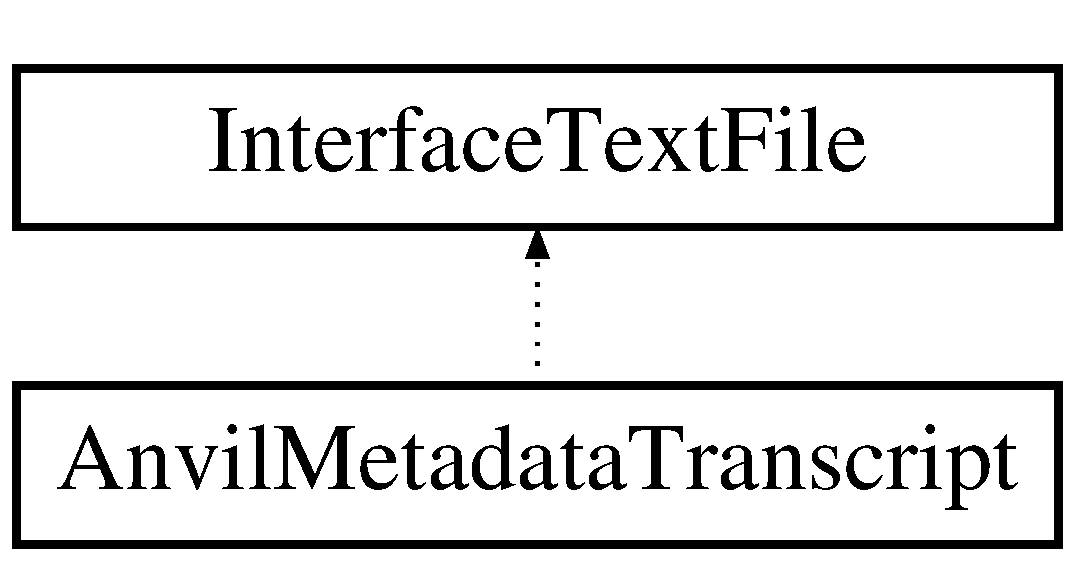
\includegraphics[height=2.000000cm]{class_anvil_metadata_transcript}
\end{center}
\end{figure}
\subsection*{Static Public Member Functions}
\begin{DoxyCompactItemize}
\item 
\mbox{\Hypertarget{class_anvil_metadata_transcript_af9df94e4175f6c841a5d96436294315f}\label{class_anvil_metadata_transcript_af9df94e4175f6c841a5d96436294315f}} 
static bool {\bfseries load} (const Q\+String \&filename, \hyperlink{class_corpus}{Corpus} $\ast$corpus)
\item 
\mbox{\Hypertarget{class_anvil_metadata_transcript_ab39806d466bc019d679de3aecad0d831}\label{class_anvil_metadata_transcript_ab39806d466bc019d679de3aecad0d831}} 
static bool {\bfseries save} (const Q\+String \&filename, \hyperlink{class_corpus}{Corpus} $\ast$corpus)
\end{DoxyCompactItemize}


The documentation for this class was generated from the following files\+:\begin{DoxyCompactItemize}
\item 
/home/george/\+Develop/\+Praaline\+Py/praaline-\/core/interfaces/anvil/Anvil\+Metadata\+Transcript.\+h\item 
/home/george/\+Develop/\+Praaline\+Py/praaline-\/core/interfaces/anvil/Anvil\+Metadata\+Transcript.\+cpp\end{DoxyCompactItemize}

\hypertarget{class_q_sql_migrator_1_1_commands_1_1_base_command}{}\section{Q\+Sql\+Migrator\+:\+:Commands\+:\+:Base\+Command Class Reference}
\label{class_q_sql_migrator_1_1_commands_1_1_base_command}\index{Q\+Sql\+Migrator\+::\+Commands\+::\+Base\+Command@{Q\+Sql\+Migrator\+::\+Commands\+::\+Base\+Command}}


abstract class for value object representing all kinds of commands  




{\ttfamily \#include $<$Base\+Command.\+h$>$}

Inheritance diagram for Q\+Sql\+Migrator\+:\+:Commands\+:\+:Base\+Command\+:\begin{figure}[H]
\begin{center}
\leavevmode
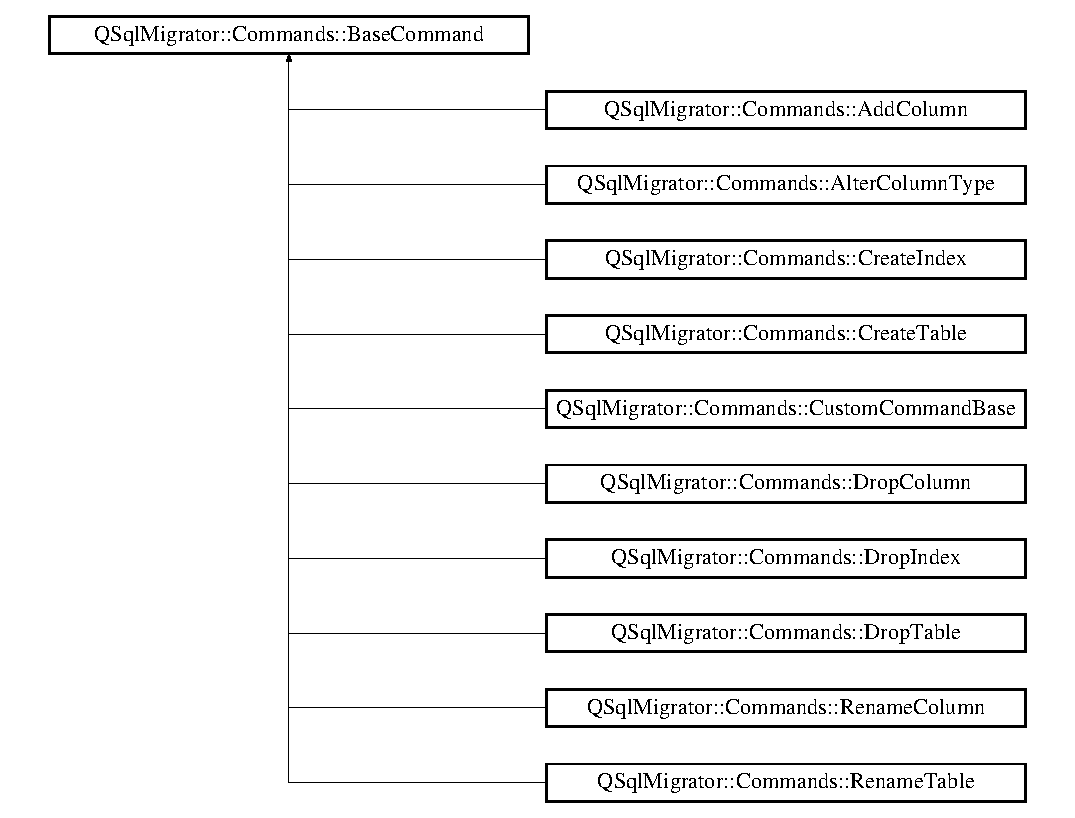
\includegraphics[height=10.547945cm]{class_q_sql_migrator_1_1_commands_1_1_base_command}
\end{center}
\end{figure}
\subsection*{Public Member Functions}
\begin{DoxyCompactItemize}
\item 
\mbox{\Hypertarget{class_q_sql_migrator_1_1_commands_1_1_base_command_a094fb40f8e1b3b4a92ed45f2a3e2265c}\label{class_q_sql_migrator_1_1_commands_1_1_base_command_a094fb40f8e1b3b4a92ed45f2a3e2265c}} 
{\bfseries Base\+Command} (const Q\+String \&name)
\item 
\mbox{\Hypertarget{class_q_sql_migrator_1_1_commands_1_1_base_command_a6d19144ca137f08f5abd4b3bcd684ffd}\label{class_q_sql_migrator_1_1_commands_1_1_base_command_a6d19144ca137f08f5abd4b3bcd684ffd}} 
const Q\+String \& {\bfseries name} () const
\item 
\mbox{\Hypertarget{class_q_sql_migrator_1_1_commands_1_1_base_command_a8ea5d829d9c2a7bb5f79652cbf76c53d}\label{class_q_sql_migrator_1_1_commands_1_1_base_command_a8ea5d829d9c2a7bb5f79652cbf76c53d}} 
virtual Command\+Ptr {\bfseries reverse} () const =0
\end{DoxyCompactItemize}


\subsection{Detailed Description}
abstract class for value object representing all kinds of commands 

The documentation for this class was generated from the following files\+:\begin{DoxyCompactItemize}
\item 
/home/george/\+Develop/\+Praaline\+Py/praaline-\/core/\+Q\+Sql\+Migrator/\+Commands/Base\+Command.\+h\item 
/home/george/\+Develop/\+Praaline\+Py/praaline-\/core/\+Q\+Sql\+Migrator/\+Commands/Base\+Command.\+cpp\end{DoxyCompactItemize}

\hypertarget{class_q_sql_migrator_1_1_command_execution_1_1_base_command_execution_service}{}\section{Q\+Sql\+Migrator\+:\+:Command\+Execution\+:\+:Base\+Command\+Execution\+Service Class Reference}
\label{class_q_sql_migrator_1_1_command_execution_1_1_base_command_execution_service}\index{Q\+Sql\+Migrator\+::\+Command\+Execution\+::\+Base\+Command\+Execution\+Service@{Q\+Sql\+Migrator\+::\+Command\+Execution\+::\+Base\+Command\+Execution\+Service}}
Inheritance diagram for Q\+Sql\+Migrator\+:\+:Command\+Execution\+:\+:Base\+Command\+Execution\+Service\+:\begin{figure}[H]
\begin{center}
\leavevmode
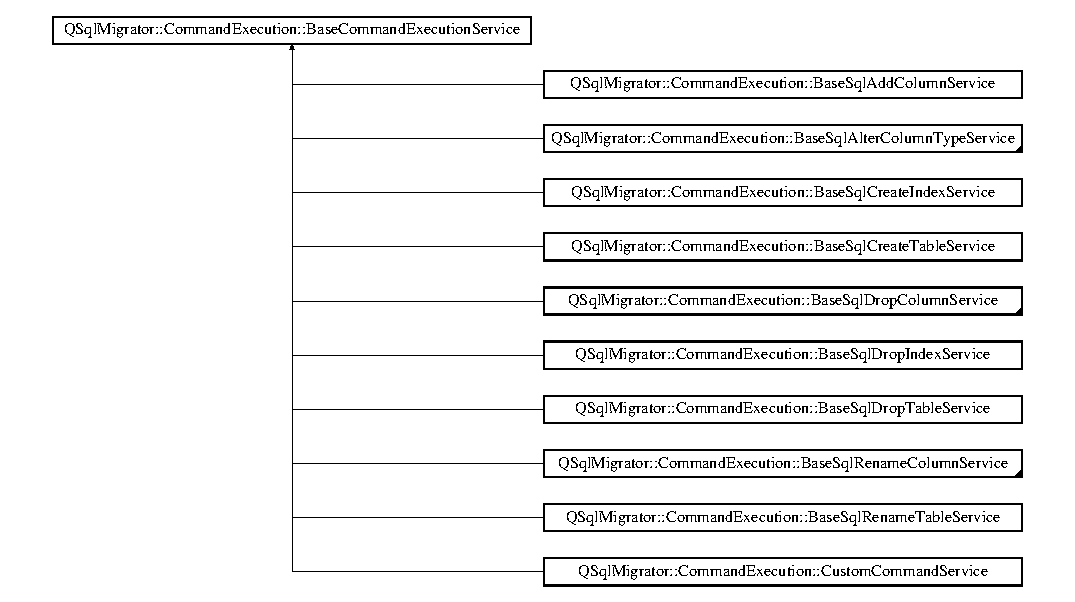
\includegraphics[height=7.642680cm]{class_q_sql_migrator_1_1_command_execution_1_1_base_command_execution_service}
\end{center}
\end{figure}
\subsection*{Public Member Functions}
\begin{DoxyCompactItemize}
\item 
\mbox{\Hypertarget{class_q_sql_migrator_1_1_command_execution_1_1_base_command_execution_service_ac2ed59b8b704834c65dcf7bb84cc684f}\label{class_q_sql_migrator_1_1_command_execution_1_1_base_command_execution_service_ac2ed59b8b704834c65dcf7bb84cc684f}} 
virtual const Q\+String \& {\bfseries command\+Type} () const =0
\item 
\mbox{\Hypertarget{class_q_sql_migrator_1_1_command_execution_1_1_base_command_execution_service_a294a781becad841fd56f8d92a6d540c1}\label{class_q_sql_migrator_1_1_command_execution_1_1_base_command_execution_service_a294a781becad841fd56f8d92a6d540c1}} 
virtual bool {\bfseries execute} (const Commands\+::\+Const\+Command\+Ptr \&command, \hyperlink{class_q_sql_migrator_1_1_command_execution_1_1_command_execution_context}{Command\+Execution\+Context} \&context) const =0
\item 
\mbox{\Hypertarget{class_q_sql_migrator_1_1_command_execution_1_1_base_command_execution_service_a298c998f3df57ba9d9f22438db1ccade}\label{class_q_sql_migrator_1_1_command_execution_1_1_base_command_execution_service_a298c998f3df57ba9d9f22438db1ccade}} 
virtual bool {\bfseries is\+Valid} (const Commands\+::\+Const\+Command\+Ptr \&command, const \hyperlink{class_q_sql_migrator_1_1_command_execution_1_1_command_execution_context}{Command\+Execution\+Context} \&context) const =0
\end{DoxyCompactItemize}
\subsection*{Static Protected Member Functions}
\begin{DoxyCompactItemize}
\item 
\mbox{\Hypertarget{class_q_sql_migrator_1_1_command_execution_1_1_base_command_execution_service_ab02914d7a5e928634ab9071fdce96484}\label{class_q_sql_migrator_1_1_command_execution_1_1_base_command_execution_service_ab02914d7a5e928634ab9071fdce96484}} 
static bool {\bfseries execute\+Query} (const Q\+String \&query\+String, const \hyperlink{class_q_sql_migrator_1_1_command_execution_1_1_command_execution_context}{Command\+Execution\+Context} \&context)
\end{DoxyCompactItemize}


The documentation for this class was generated from the following files\+:\begin{DoxyCompactItemize}
\item 
/home/george/\+Develop/\+Praaline\+Py/praaline-\/core/\+Q\+Sql\+Migrator/\+Command\+Execution/Base\+Command\+Execution\+Service.\+h\item 
/home/george/\+Develop/\+Praaline\+Py/praaline-\/core/\+Q\+Sql\+Migrator/\+Command\+Execution/Base\+Command\+Execution\+Service.\+cpp\end{DoxyCompactItemize}

\hypertarget{class_q_sql_migrator_1_1_migration_tracker_1_1_base_migration_table_service}{}\section{Q\+Sql\+Migrator\+:\+:Migration\+Tracker\+:\+:Base\+Migration\+Table\+Service Class Reference}
\label{class_q_sql_migrator_1_1_migration_tracker_1_1_base_migration_table_service}\index{Q\+Sql\+Migrator\+::\+Migration\+Tracker\+::\+Base\+Migration\+Table\+Service@{Q\+Sql\+Migrator\+::\+Migration\+Tracker\+::\+Base\+Migration\+Table\+Service}}


Implementation of the successfully executed migration tracking through an sql databse table.  




{\ttfamily \#include $<$Base\+Migration\+Table\+Service.\+h$>$}

Inheritance diagram for Q\+Sql\+Migrator\+:\+:Migration\+Tracker\+:\+:Base\+Migration\+Table\+Service\+:\begin{figure}[H]
\begin{center}
\leavevmode
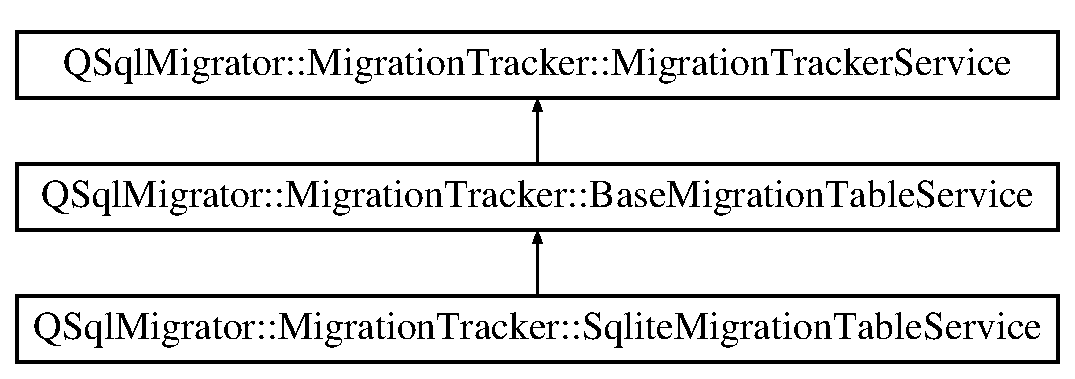
\includegraphics[height=3.000000cm]{class_q_sql_migrator_1_1_migration_tracker_1_1_base_migration_table_service}
\end{center}
\end{figure}
\subsection*{Public Member Functions}
\begin{DoxyCompactItemize}
\item 
bool \hyperlink{class_q_sql_migrator_1_1_migration_tracker_1_1_base_migration_table_service_aea5fa9e4804a436221180560efeab253}{can\+Revert\+Strucutural\+Changes\+Using\+Transactions} () const Q\+\_\+\+D\+E\+C\+L\+\_\+\+O\+V\+E\+R\+R\+I\+DE
\item 
bool \hyperlink{class_q_sql_migrator_1_1_migration_tracker_1_1_base_migration_table_service_afaa1f00b646de9db114a82597a40f9ea}{was\+Migration\+Executed} (const Q\+String \&migration\+Name, const \hyperlink{class_q_sql_migrator_1_1_command_execution_1_1_command_execution_context}{Command\+Execution\+::\+Command\+Execution\+Context} \&context) const Q\+\_\+\+D\+E\+C\+L\+\_\+\+O\+V\+E\+R\+R\+I\+DE
\item 
Q\+String\+List \hyperlink{class_q_sql_migrator_1_1_migration_tracker_1_1_base_migration_table_service_a1105240b456db9f85c2fc2866582a292}{migration\+List} (const \hyperlink{class_q_sql_migrator_1_1_command_execution_1_1_command_execution_context}{Command\+Execution\+::\+Command\+Execution\+Context} \&context) const Q\+\_\+\+D\+E\+C\+L\+\_\+\+O\+V\+E\+R\+R\+I\+DE
\item 
bool \hyperlink{class_q_sql_migrator_1_1_migration_tracker_1_1_base_migration_table_service_a0acf906f43678d623984e334fe43a11a}{add\+Migration} (const Q\+String \&migration\+Name, const \hyperlink{class_q_sql_migrator_1_1_command_execution_1_1_command_execution_context}{Command\+Execution\+::\+Command\+Execution\+Context} \&context) const Q\+\_\+\+D\+E\+C\+L\+\_\+\+O\+V\+E\+R\+R\+I\+DE
\item 
bool \hyperlink{class_q_sql_migrator_1_1_migration_tracker_1_1_base_migration_table_service_a2b0bf914a7672e5540b7b003cd378aaf}{remove\+Migration} (const Q\+String \&migration\+Name, const \hyperlink{class_q_sql_migrator_1_1_command_execution_1_1_command_execution_context}{Command\+Execution\+::\+Command\+Execution\+Context} \&context) const Q\+\_\+\+D\+E\+C\+L\+\_\+\+O\+V\+E\+R\+R\+I\+DE
\item 
bool \hyperlink{class_q_sql_migrator_1_1_migration_tracker_1_1_base_migration_table_service_a76bec328f72c8fc91002cc285731332c}{prepare} (const \hyperlink{class_q_sql_migrator_1_1_migration_execution_1_1_migration_execution_context}{Migration\+Execution\+::\+Migration\+Execution\+Context} \&context) const Q\+\_\+\+D\+E\+C\+L\+\_\+\+O\+V\+E\+R\+R\+I\+DE
\end{DoxyCompactItemize}


\subsection{Detailed Description}
Implementation of the successfully executed migration tracking through an sql databse table. 

\subsection{Member Function Documentation}
\mbox{\Hypertarget{class_q_sql_migrator_1_1_migration_tracker_1_1_base_migration_table_service_a0acf906f43678d623984e334fe43a11a}\label{class_q_sql_migrator_1_1_migration_tracker_1_1_base_migration_table_service_a0acf906f43678d623984e334fe43a11a}} 
\index{Q\+Sql\+Migrator\+::\+Migration\+Tracker\+::\+Base\+Migration\+Table\+Service@{Q\+Sql\+Migrator\+::\+Migration\+Tracker\+::\+Base\+Migration\+Table\+Service}!add\+Migration@{add\+Migration}}
\index{add\+Migration@{add\+Migration}!Q\+Sql\+Migrator\+::\+Migration\+Tracker\+::\+Base\+Migration\+Table\+Service@{Q\+Sql\+Migrator\+::\+Migration\+Tracker\+::\+Base\+Migration\+Table\+Service}}
\subsubsection{\texorpdfstring{add\+Migration()}{addMigration()}}
{\footnotesize\ttfamily bool Q\+Sql\+Migrator\+::\+Migration\+Tracker\+::\+Base\+Migration\+Table\+Service\+::add\+Migration (\begin{DoxyParamCaption}\item[{const Q\+String \&}]{migration\+Name,  }\item[{const \hyperlink{class_q_sql_migrator_1_1_command_execution_1_1_command_execution_context}{Command\+Execution\+::\+Command\+Execution\+Context} \&}]{context }\end{DoxyParamCaption}) const\hspace{0.3cm}{\ttfamily [virtual]}}

\begin{DoxyReturn}{Returns}
true, if it was able to sucessfully record that the migrations was executed 
\end{DoxyReturn}


Implements \hyperlink{class_q_sql_migrator_1_1_migration_tracker_1_1_migration_tracker_service_ad9bc087a72a4535e81812a0069dbaa6a}{Q\+Sql\+Migrator\+::\+Migration\+Tracker\+::\+Migration\+Tracker\+Service}.

\mbox{\Hypertarget{class_q_sql_migrator_1_1_migration_tracker_1_1_base_migration_table_service_aea5fa9e4804a436221180560efeab253}\label{class_q_sql_migrator_1_1_migration_tracker_1_1_base_migration_table_service_aea5fa9e4804a436221180560efeab253}} 
\index{Q\+Sql\+Migrator\+::\+Migration\+Tracker\+::\+Base\+Migration\+Table\+Service@{Q\+Sql\+Migrator\+::\+Migration\+Tracker\+::\+Base\+Migration\+Table\+Service}!can\+Revert\+Strucutural\+Changes\+Using\+Transactions@{can\+Revert\+Strucutural\+Changes\+Using\+Transactions}}
\index{can\+Revert\+Strucutural\+Changes\+Using\+Transactions@{can\+Revert\+Strucutural\+Changes\+Using\+Transactions}!Q\+Sql\+Migrator\+::\+Migration\+Tracker\+::\+Base\+Migration\+Table\+Service@{Q\+Sql\+Migrator\+::\+Migration\+Tracker\+::\+Base\+Migration\+Table\+Service}}
\subsubsection{\texorpdfstring{can\+Revert\+Strucutural\+Changes\+Using\+Transactions()}{canRevertStrucuturalChangesUsingTransactions()}}
{\footnotesize\ttfamily bool Q\+Sql\+Migrator\+::\+Migration\+Tracker\+::\+Base\+Migration\+Table\+Service\+::can\+Revert\+Strucutural\+Changes\+Using\+Transactions (\begin{DoxyParamCaption}{ }\end{DoxyParamCaption}) const\hspace{0.3cm}{\ttfamily [virtual]}}

\begin{DoxyReturn}{Returns}
true if transactions can revert changes to table structures 
\end{DoxyReturn}


Implements \hyperlink{class_q_sql_migrator_1_1_migration_tracker_1_1_migration_tracker_service_a539b5fe686ffd6ae6577c046201f0df3}{Q\+Sql\+Migrator\+::\+Migration\+Tracker\+::\+Migration\+Tracker\+Service}.



Reimplemented in \hyperlink{class_q_sql_migrator_1_1_migration_tracker_1_1_sqlite_migration_table_service_a6d2f747ce2a599033dee174f8e996fff}{Q\+Sql\+Migrator\+::\+Migration\+Tracker\+::\+Sqlite\+Migration\+Table\+Service}.

\mbox{\Hypertarget{class_q_sql_migrator_1_1_migration_tracker_1_1_base_migration_table_service_a1105240b456db9f85c2fc2866582a292}\label{class_q_sql_migrator_1_1_migration_tracker_1_1_base_migration_table_service_a1105240b456db9f85c2fc2866582a292}} 
\index{Q\+Sql\+Migrator\+::\+Migration\+Tracker\+::\+Base\+Migration\+Table\+Service@{Q\+Sql\+Migrator\+::\+Migration\+Tracker\+::\+Base\+Migration\+Table\+Service}!migration\+List@{migration\+List}}
\index{migration\+List@{migration\+List}!Q\+Sql\+Migrator\+::\+Migration\+Tracker\+::\+Base\+Migration\+Table\+Service@{Q\+Sql\+Migrator\+::\+Migration\+Tracker\+::\+Base\+Migration\+Table\+Service}}
\subsubsection{\texorpdfstring{migration\+List()}{migrationList()}}
{\footnotesize\ttfamily Q\+String\+List Q\+Sql\+Migrator\+::\+Migration\+Tracker\+::\+Base\+Migration\+Table\+Service\+::migration\+List (\begin{DoxyParamCaption}\item[{const \hyperlink{class_q_sql_migrator_1_1_command_execution_1_1_command_execution_context}{Command\+Execution\+::\+Command\+Execution\+Context} \&}]{context }\end{DoxyParamCaption}) const\hspace{0.3cm}{\ttfamily [virtual]}}

\begin{DoxyReturn}{Returns}
a list of all tracked successful migration executions 
\end{DoxyReturn}


Implements \hyperlink{class_q_sql_migrator_1_1_migration_tracker_1_1_migration_tracker_service_a5de22e070fc1b4f487dbe256e1c874ef}{Q\+Sql\+Migrator\+::\+Migration\+Tracker\+::\+Migration\+Tracker\+Service}.

\mbox{\Hypertarget{class_q_sql_migrator_1_1_migration_tracker_1_1_base_migration_table_service_a76bec328f72c8fc91002cc285731332c}\label{class_q_sql_migrator_1_1_migration_tracker_1_1_base_migration_table_service_a76bec328f72c8fc91002cc285731332c}} 
\index{Q\+Sql\+Migrator\+::\+Migration\+Tracker\+::\+Base\+Migration\+Table\+Service@{Q\+Sql\+Migrator\+::\+Migration\+Tracker\+::\+Base\+Migration\+Table\+Service}!prepare@{prepare}}
\index{prepare@{prepare}!Q\+Sql\+Migrator\+::\+Migration\+Tracker\+::\+Base\+Migration\+Table\+Service@{Q\+Sql\+Migrator\+::\+Migration\+Tracker\+::\+Base\+Migration\+Table\+Service}}
\subsubsection{\texorpdfstring{prepare()}{prepare()}}
{\footnotesize\ttfamily bool Q\+Sql\+Migrator\+::\+Migration\+Tracker\+::\+Base\+Migration\+Table\+Service\+::prepare (\begin{DoxyParamCaption}\item[{const \hyperlink{class_q_sql_migrator_1_1_migration_execution_1_1_migration_execution_context}{Migration\+Execution\+::\+Migration\+Execution\+Context} \&}]{context }\end{DoxyParamCaption}) const\hspace{0.3cm}{\ttfamily [virtual]}}

\begin{DoxyReturn}{Returns}
true, if the tracking was in place or was sucessfully prepared 
\end{DoxyReturn}


Implements \hyperlink{class_q_sql_migrator_1_1_migration_tracker_1_1_migration_tracker_service_a26dc17b23f3e2a62c9964ce46c740b57}{Q\+Sql\+Migrator\+::\+Migration\+Tracker\+::\+Migration\+Tracker\+Service}.

\mbox{\Hypertarget{class_q_sql_migrator_1_1_migration_tracker_1_1_base_migration_table_service_a2b0bf914a7672e5540b7b003cd378aaf}\label{class_q_sql_migrator_1_1_migration_tracker_1_1_base_migration_table_service_a2b0bf914a7672e5540b7b003cd378aaf}} 
\index{Q\+Sql\+Migrator\+::\+Migration\+Tracker\+::\+Base\+Migration\+Table\+Service@{Q\+Sql\+Migrator\+::\+Migration\+Tracker\+::\+Base\+Migration\+Table\+Service}!remove\+Migration@{remove\+Migration}}
\index{remove\+Migration@{remove\+Migration}!Q\+Sql\+Migrator\+::\+Migration\+Tracker\+::\+Base\+Migration\+Table\+Service@{Q\+Sql\+Migrator\+::\+Migration\+Tracker\+::\+Base\+Migration\+Table\+Service}}
\subsubsection{\texorpdfstring{remove\+Migration()}{removeMigration()}}
{\footnotesize\ttfamily bool Q\+Sql\+Migrator\+::\+Migration\+Tracker\+::\+Base\+Migration\+Table\+Service\+::remove\+Migration (\begin{DoxyParamCaption}\item[{const Q\+String \&}]{migration\+Name,  }\item[{const \hyperlink{class_q_sql_migrator_1_1_command_execution_1_1_command_execution_context}{Command\+Execution\+::\+Command\+Execution\+Context} \&}]{context }\end{DoxyParamCaption}) const\hspace{0.3cm}{\ttfamily [virtual]}}

\begin{DoxyReturn}{Returns}
true, if it was able to sucessfully remove a migration from the tracked successfully executed migrations 
\end{DoxyReturn}


Implements \hyperlink{class_q_sql_migrator_1_1_migration_tracker_1_1_migration_tracker_service_a3041c2cb0027e6a40639ce4c47482c17}{Q\+Sql\+Migrator\+::\+Migration\+Tracker\+::\+Migration\+Tracker\+Service}.

\mbox{\Hypertarget{class_q_sql_migrator_1_1_migration_tracker_1_1_base_migration_table_service_afaa1f00b646de9db114a82597a40f9ea}\label{class_q_sql_migrator_1_1_migration_tracker_1_1_base_migration_table_service_afaa1f00b646de9db114a82597a40f9ea}} 
\index{Q\+Sql\+Migrator\+::\+Migration\+Tracker\+::\+Base\+Migration\+Table\+Service@{Q\+Sql\+Migrator\+::\+Migration\+Tracker\+::\+Base\+Migration\+Table\+Service}!was\+Migration\+Executed@{was\+Migration\+Executed}}
\index{was\+Migration\+Executed@{was\+Migration\+Executed}!Q\+Sql\+Migrator\+::\+Migration\+Tracker\+::\+Base\+Migration\+Table\+Service@{Q\+Sql\+Migrator\+::\+Migration\+Tracker\+::\+Base\+Migration\+Table\+Service}}
\subsubsection{\texorpdfstring{was\+Migration\+Executed()}{wasMigrationExecuted()}}
{\footnotesize\ttfamily bool Q\+Sql\+Migrator\+::\+Migration\+Tracker\+::\+Base\+Migration\+Table\+Service\+::was\+Migration\+Executed (\begin{DoxyParamCaption}\item[{const Q\+String \&}]{migration\+Name,  }\item[{const \hyperlink{class_q_sql_migrator_1_1_command_execution_1_1_command_execution_context}{Command\+Execution\+::\+Command\+Execution\+Context} \&}]{context }\end{DoxyParamCaption}) const\hspace{0.3cm}{\ttfamily [virtual]}}

\begin{DoxyReturn}{Returns}
true if the specified migrations was tracked as successfully executed 
\end{DoxyReturn}


Implements \hyperlink{class_q_sql_migrator_1_1_migration_tracker_1_1_migration_tracker_service_a8bb56a82aeefab574a0d7eb2dd5112e5}{Q\+Sql\+Migrator\+::\+Migration\+Tracker\+::\+Migration\+Tracker\+Service}.



The documentation for this class was generated from the following files\+:\begin{DoxyCompactItemize}
\item 
/home/george/\+Develop/\+Praaline\+Py/praaline-\/core/\+Q\+Sql\+Migrator/\+Base\+Sql\+Migrator/\+Migration\+Tracker/Base\+Migration\+Table\+Service.\+h\item 
/home/george/\+Develop/\+Praaline\+Py/praaline-\/core/\+Q\+Sql\+Migrator/\+Base\+Sql\+Migrator/\+Migration\+Tracker/Base\+Migration\+Table\+Service.\+cpp\end{DoxyCompactItemize}

\hypertarget{class_q_sql_migrator_1_1_command_execution_1_1_base_sql_add_column_service}{}\section{Q\+Sql\+Migrator\+:\+:Command\+Execution\+:\+:Base\+Sql\+Add\+Column\+Service Class Reference}
\label{class_q_sql_migrator_1_1_command_execution_1_1_base_sql_add_column_service}\index{Q\+Sql\+Migrator\+::\+Command\+Execution\+::\+Base\+Sql\+Add\+Column\+Service@{Q\+Sql\+Migrator\+::\+Command\+Execution\+::\+Base\+Sql\+Add\+Column\+Service}}
Inheritance diagram for Q\+Sql\+Migrator\+:\+:Command\+Execution\+:\+:Base\+Sql\+Add\+Column\+Service\+:\begin{figure}[H]
\begin{center}
\leavevmode
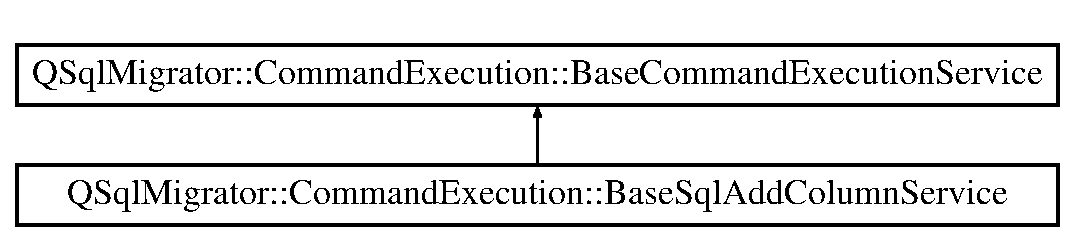
\includegraphics[height=2.000000cm]{class_q_sql_migrator_1_1_command_execution_1_1_base_sql_add_column_service}
\end{center}
\end{figure}
\subsection*{Public Member Functions}
\begin{DoxyCompactItemize}
\item 
\mbox{\Hypertarget{class_q_sql_migrator_1_1_command_execution_1_1_base_sql_add_column_service_ae60b5ac342c59c4f74f7743f9dfa1f57}\label{class_q_sql_migrator_1_1_command_execution_1_1_base_sql_add_column_service_ae60b5ac342c59c4f74f7743f9dfa1f57}} 
const Q\+String \& {\bfseries command\+Type} () const
\item 
\mbox{\Hypertarget{class_q_sql_migrator_1_1_command_execution_1_1_base_sql_add_column_service_ab6c7105ff8e6e2e2c4b37ce6a021bd69}\label{class_q_sql_migrator_1_1_command_execution_1_1_base_sql_add_column_service_ab6c7105ff8e6e2e2c4b37ce6a021bd69}} 
bool {\bfseries execute} (const Commands\+::\+Const\+Command\+Ptr \&command, \hyperlink{class_q_sql_migrator_1_1_command_execution_1_1_command_execution_context}{Command\+Execution\+::\+Command\+Execution\+Context} \&context) const
\item 
\mbox{\Hypertarget{class_q_sql_migrator_1_1_command_execution_1_1_base_sql_add_column_service_a78859e1028b58cf227edd0ad683237e4}\label{class_q_sql_migrator_1_1_command_execution_1_1_base_sql_add_column_service_a78859e1028b58cf227edd0ad683237e4}} 
bool {\bfseries is\+Valid} (const Commands\+::\+Const\+Command\+Ptr \&command, const \hyperlink{class_q_sql_migrator_1_1_command_execution_1_1_command_execution_context}{Command\+Execution\+::\+Command\+Execution\+Context} \&context) const
\end{DoxyCompactItemize}
\subsection*{Static Public Member Functions}
\begin{DoxyCompactItemize}
\item 
\mbox{\Hypertarget{class_q_sql_migrator_1_1_command_execution_1_1_base_sql_add_column_service_ab703a3c3cd97fb936c7c395f117163d8}\label{class_q_sql_migrator_1_1_command_execution_1_1_base_sql_add_column_service_ab703a3c3cd97fb936c7c395f117163d8}} 
static bool {\bfseries execute} (const \hyperlink{class_q_sql_migrator_1_1_commands_1_1_add_column}{Commands\+::\+Add\+Column} \&add\+Column, const \hyperlink{class_q_sql_migrator_1_1_command_execution_1_1_command_execution_context}{Command\+Execution\+::\+Command\+Execution\+Context} \&context)
\end{DoxyCompactItemize}
\subsection*{Additional Inherited Members}


The documentation for this class was generated from the following files\+:\begin{DoxyCompactItemize}
\item 
/home/george/\+Develop/\+Praaline\+Py/praaline-\/core/\+Q\+Sql\+Migrator/\+Base\+Sql\+Migrator/\+Command\+Execution/Base\+Sql\+Add\+Column\+Service.\+h\item 
/home/george/\+Develop/\+Praaline\+Py/praaline-\/core/\+Q\+Sql\+Migrator/\+Base\+Sql\+Migrator/\+Command\+Execution/Base\+Sql\+Add\+Column\+Service.\+cpp\end{DoxyCompactItemize}

\hypertarget{class_q_sql_migrator_1_1_command_execution_1_1_base_sql_alter_column_type_service}{}\section{Q\+Sql\+Migrator\+:\+:Command\+Execution\+:\+:Base\+Sql\+Alter\+Column\+Type\+Service Class Reference}
\label{class_q_sql_migrator_1_1_command_execution_1_1_base_sql_alter_column_type_service}\index{Q\+Sql\+Migrator\+::\+Command\+Execution\+::\+Base\+Sql\+Alter\+Column\+Type\+Service@{Q\+Sql\+Migrator\+::\+Command\+Execution\+::\+Base\+Sql\+Alter\+Column\+Type\+Service}}
Inheritance diagram for Q\+Sql\+Migrator\+:\+:Command\+Execution\+:\+:Base\+Sql\+Alter\+Column\+Type\+Service\+:\begin{figure}[H]
\begin{center}
\leavevmode
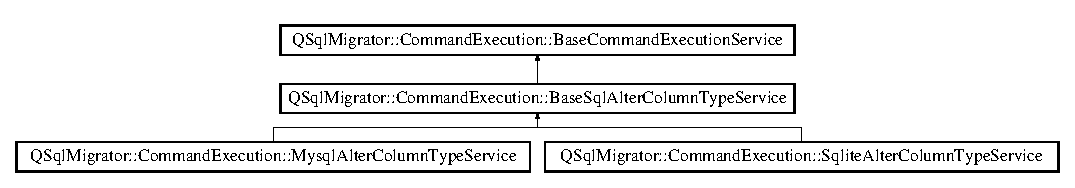
\includegraphics[height=2.084367cm]{class_q_sql_migrator_1_1_command_execution_1_1_base_sql_alter_column_type_service}
\end{center}
\end{figure}
\subsection*{Public Member Functions}
\begin{DoxyCompactItemize}
\item 
\mbox{\Hypertarget{class_q_sql_migrator_1_1_command_execution_1_1_base_sql_alter_column_type_service_a4ae10db4b241f5b65ecfffb01bcb5da7}\label{class_q_sql_migrator_1_1_command_execution_1_1_base_sql_alter_column_type_service_a4ae10db4b241f5b65ecfffb01bcb5da7}} 
const Q\+String \& {\bfseries command\+Type} () const
\item 
\mbox{\Hypertarget{class_q_sql_migrator_1_1_command_execution_1_1_base_sql_alter_column_type_service_a8e56cdd17ad78d954ce178d498771a26}\label{class_q_sql_migrator_1_1_command_execution_1_1_base_sql_alter_column_type_service_a8e56cdd17ad78d954ce178d498771a26}} 
bool {\bfseries execute} (const Commands\+::\+Const\+Command\+Ptr \&command, \hyperlink{class_q_sql_migrator_1_1_command_execution_1_1_command_execution_context}{Command\+Execution\+::\+Command\+Execution\+Context} \&context) const
\item 
\mbox{\Hypertarget{class_q_sql_migrator_1_1_command_execution_1_1_base_sql_alter_column_type_service_a4806fc79495db984bfb3e5719e5fe005}\label{class_q_sql_migrator_1_1_command_execution_1_1_base_sql_alter_column_type_service_a4806fc79495db984bfb3e5719e5fe005}} 
bool {\bfseries is\+Valid} (const Commands\+::\+Const\+Command\+Ptr \&command, const \hyperlink{class_q_sql_migrator_1_1_command_execution_1_1_command_execution_context}{Command\+Execution\+::\+Command\+Execution\+Context} \&context) const
\end{DoxyCompactItemize}
\subsection*{Static Public Member Functions}
\begin{DoxyCompactItemize}
\item 
\mbox{\Hypertarget{class_q_sql_migrator_1_1_command_execution_1_1_base_sql_alter_column_type_service_ac9d253c83ee0341e445ad197734e132f}\label{class_q_sql_migrator_1_1_command_execution_1_1_base_sql_alter_column_type_service_ac9d253c83ee0341e445ad197734e132f}} 
static bool {\bfseries execute} (const \hyperlink{class_q_sql_migrator_1_1_commands_1_1_alter_column_type}{Commands\+::\+Alter\+Column\+Type} \&alter\+Column\+Type, const \hyperlink{class_q_sql_migrator_1_1_command_execution_1_1_command_execution_context}{Command\+Execution\+::\+Command\+Execution\+Context} \&context)
\end{DoxyCompactItemize}
\subsection*{Additional Inherited Members}


The documentation for this class was generated from the following files\+:\begin{DoxyCompactItemize}
\item 
/home/george/\+Develop/\+Praaline\+Py/praaline-\/core/\+Q\+Sql\+Migrator/\+Base\+Sql\+Migrator/\+Command\+Execution/Base\+Sql\+Alter\+Column\+Type\+Service.\+h\item 
/home/george/\+Develop/\+Praaline\+Py/praaline-\/core/\+Q\+Sql\+Migrator/\+Base\+Sql\+Migrator/\+Command\+Execution/Base\+Sql\+Alter\+Column\+Type\+Service.\+cpp\end{DoxyCompactItemize}

\hypertarget{class_q_sql_migrator_1_1_helper_1_1_base_sql_column_service}{}\section{Q\+Sql\+Migrator\+:\+:Helper\+:\+:Base\+Sql\+Column\+Service Class Reference}
\label{class_q_sql_migrator_1_1_helper_1_1_base_sql_column_service}\index{Q\+Sql\+Migrator\+::\+Helper\+::\+Base\+Sql\+Column\+Service@{Q\+Sql\+Migrator\+::\+Helper\+::\+Base\+Sql\+Column\+Service}}
Inheritance diagram for Q\+Sql\+Migrator\+:\+:Helper\+:\+:Base\+Sql\+Column\+Service\+:\begin{figure}[H]
\begin{center}
\leavevmode
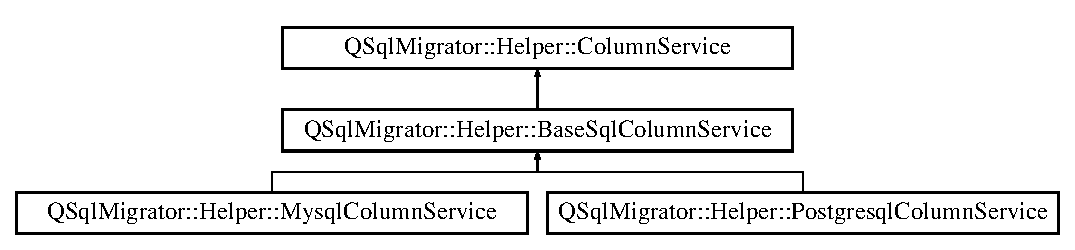
\includegraphics[height=2.906574cm]{class_q_sql_migrator_1_1_helper_1_1_base_sql_column_service}
\end{center}
\end{figure}
\subsection*{Public Types}
\begin{DoxyCompactItemize}
\item 
\mbox{\Hypertarget{class_q_sql_migrator_1_1_helper_1_1_base_sql_column_service_a9ef1b6bd6c0eaeb2ed998fc1313e07cc}\label{class_q_sql_migrator_1_1_helper_1_1_base_sql_column_service_a9ef1b6bd6c0eaeb2ed998fc1313e07cc}} 
typedef std\+::function$<$ void(const Q\+String \&type) $>$ {\bfseries String\+Output\+Function}
\end{DoxyCompactItemize}
\subsection*{Public Member Functions}
\begin{DoxyCompactItemize}
\item 
\mbox{\Hypertarget{class_q_sql_migrator_1_1_helper_1_1_base_sql_column_service_a2a7e948e520d3da4eaf308d2574675f7}\label{class_q_sql_migrator_1_1_helper_1_1_base_sql_column_service_a2a7e948e520d3da4eaf308d2574675f7}} 
{\bfseries Base\+Sql\+Column\+Service} (const \hyperlink{class_q_sql_migrator_1_1_helper_1_1_type_mapper_service}{Type\+Mapper\+Service} \&type\+Mapper\+Service)
\item 
\mbox{\Hypertarget{class_q_sql_migrator_1_1_helper_1_1_base_sql_column_service_ac27cec78ddb481482c811ab5535b6da6}\label{class_q_sql_migrator_1_1_helper_1_1_base_sql_column_service_ac27cec78ddb481482c811ab5535b6da6}} 
virtual Q\+String {\bfseries build\+Column\+Type\+Sql} (const \hyperlink{class_q_sql_migrator_1_1_structure_1_1_column}{Structure\+::\+Column} \&column) const
\item 
\mbox{\Hypertarget{class_q_sql_migrator_1_1_helper_1_1_base_sql_column_service_ac4654897bbc706f81e458e4e134ae36d}\label{class_q_sql_migrator_1_1_helper_1_1_base_sql_column_service_ac4654897bbc706f81e458e4e134ae36d}} 
virtual void {\bfseries build\+Column\+Options\+Sql} (const \hyperlink{class_q_sql_migrator_1_1_structure_1_1_column}{Structure\+::\+Column} \&column, const String\+Output\+Function \&add\+Option) const
\item 
\mbox{\Hypertarget{class_q_sql_migrator_1_1_helper_1_1_base_sql_column_service_a46b338ad94cebfb2b408ec0a5977eedb}\label{class_q_sql_migrator_1_1_helper_1_1_base_sql_column_service_a46b338ad94cebfb2b408ec0a5977eedb}} 
Q\+String {\bfseries generate\+Column\+Definition\+Sql} (const \hyperlink{class_q_sql_migrator_1_1_structure_1_1_column}{Structure\+::\+Column} \&column) const Q\+\_\+\+D\+E\+C\+L\+\_\+\+O\+V\+E\+R\+R\+I\+DE
\item 
\mbox{\Hypertarget{class_q_sql_migrator_1_1_helper_1_1_base_sql_column_service_a1df2e7645c44a6a80d8aab242d55ceac}\label{class_q_sql_migrator_1_1_helper_1_1_base_sql_column_service_a1df2e7645c44a6a80d8aab242d55ceac}} 
Q\+String {\bfseries generate\+Columns\+Definition\+Sql} (const Q\+List$<$ \hyperlink{class_q_sql_migrator_1_1_structure_1_1_column}{Structure\+::\+Column} $>$ \&column\+List) const Q\+\_\+\+D\+E\+C\+L\+\_\+\+O\+V\+E\+R\+R\+I\+DE
\item 
\mbox{\Hypertarget{class_q_sql_migrator_1_1_helper_1_1_base_sql_column_service_acf93e8a83e2e23b8ccd83de0ea83bfdb}\label{class_q_sql_migrator_1_1_helper_1_1_base_sql_column_service_acf93e8a83e2e23b8ccd83de0ea83bfdb}} 
Q\+String {\bfseries generate\+Index\+Column\+Definition\+Sql} (const \hyperlink{class_q_sql_migrator_1_1_structure_1_1_index_1_1_column}{Structure\+::\+Index\+::\+Column} \&column) const Q\+\_\+\+D\+E\+C\+L\+\_\+\+O\+V\+E\+R\+R\+I\+DE
\item 
\mbox{\Hypertarget{class_q_sql_migrator_1_1_helper_1_1_base_sql_column_service_a650745d0a11d04226c11103bcbcba2ce}\label{class_q_sql_migrator_1_1_helper_1_1_base_sql_column_service_a650745d0a11d04226c11103bcbcba2ce}} 
Q\+String {\bfseries generate\+Index\+Columns\+Definition\+Sql} (const Structure\+::\+Index\+::\+Column\+List \&columns) const Q\+\_\+\+D\+E\+C\+L\+\_\+\+O\+V\+E\+R\+R\+I\+DE
\end{DoxyCompactItemize}
\subsection*{Protected Attributes}
\begin{DoxyCompactItemize}
\item 
\mbox{\Hypertarget{class_q_sql_migrator_1_1_helper_1_1_base_sql_column_service_a4181f6442b4a6109fb7ab4c651df5343}\label{class_q_sql_migrator_1_1_helper_1_1_base_sql_column_service_a4181f6442b4a6109fb7ab4c651df5343}} 
const \hyperlink{class_q_sql_migrator_1_1_helper_1_1_type_mapper_service}{Type\+Mapper\+Service} \& {\bfseries m\+\_\+type\+Mapper\+Service}
\end{DoxyCompactItemize}


The documentation for this class was generated from the following files\+:\begin{DoxyCompactItemize}
\item 
/home/george/\+Develop/\+Praaline\+Py/praaline-\/core/\+Q\+Sql\+Migrator/\+Base\+Sql\+Migrator/\+Helper/Base\+Sql\+Column\+Service.\+h\item 
/home/george/\+Develop/\+Praaline\+Py/praaline-\/core/\+Q\+Sql\+Migrator/\+Base\+Sql\+Migrator/\+Helper/Base\+Sql\+Column\+Service.\+cpp\end{DoxyCompactItemize}

\hypertarget{class_q_sql_migrator_1_1_command_execution_1_1_base_sql_create_index_service}{}\section{Q\+Sql\+Migrator\+:\+:Command\+Execution\+:\+:Base\+Sql\+Create\+Index\+Service Class Reference}
\label{class_q_sql_migrator_1_1_command_execution_1_1_base_sql_create_index_service}\index{Q\+Sql\+Migrator\+::\+Command\+Execution\+::\+Base\+Sql\+Create\+Index\+Service@{Q\+Sql\+Migrator\+::\+Command\+Execution\+::\+Base\+Sql\+Create\+Index\+Service}}
Inheritance diagram for Q\+Sql\+Migrator\+:\+:Command\+Execution\+:\+:Base\+Sql\+Create\+Index\+Service\+:\begin{figure}[H]
\begin{center}
\leavevmode
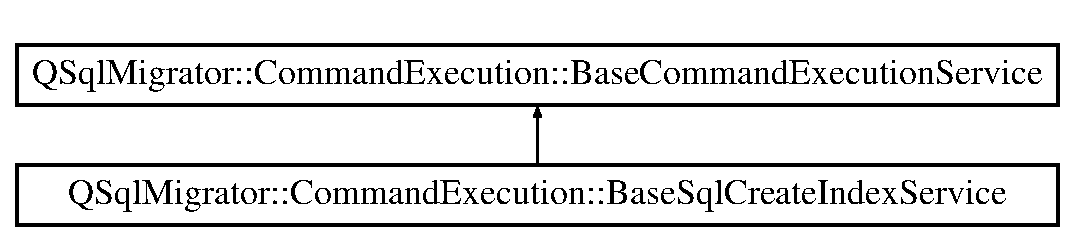
\includegraphics[height=2.000000cm]{class_q_sql_migrator_1_1_command_execution_1_1_base_sql_create_index_service}
\end{center}
\end{figure}
\subsection*{Public Member Functions}
\begin{DoxyCompactItemize}
\item 
\mbox{\Hypertarget{class_q_sql_migrator_1_1_command_execution_1_1_base_sql_create_index_service_aa4c885ce4f4967ba71149f80d0a711aa}\label{class_q_sql_migrator_1_1_command_execution_1_1_base_sql_create_index_service_aa4c885ce4f4967ba71149f80d0a711aa}} 
const Q\+String \& {\bfseries command\+Type} () const
\item 
\mbox{\Hypertarget{class_q_sql_migrator_1_1_command_execution_1_1_base_sql_create_index_service_a90f6d3a4a67e8e721184e8c8709e2550}\label{class_q_sql_migrator_1_1_command_execution_1_1_base_sql_create_index_service_a90f6d3a4a67e8e721184e8c8709e2550}} 
bool {\bfseries execute} (const Commands\+::\+Const\+Command\+Ptr \&command, \hyperlink{class_q_sql_migrator_1_1_command_execution_1_1_command_execution_context}{Command\+Execution\+::\+Command\+Execution\+Context} \&context) const
\item 
\mbox{\Hypertarget{class_q_sql_migrator_1_1_command_execution_1_1_base_sql_create_index_service_a56d2662eb7d74dfab2ebf0edcd4e388d}\label{class_q_sql_migrator_1_1_command_execution_1_1_base_sql_create_index_service_a56d2662eb7d74dfab2ebf0edcd4e388d}} 
bool {\bfseries is\+Valid} (const Commands\+::\+Const\+Command\+Ptr \&command, const \hyperlink{class_q_sql_migrator_1_1_command_execution_1_1_command_execution_context}{Command\+Execution\+::\+Command\+Execution\+Context} \&context) const
\end{DoxyCompactItemize}
\subsection*{Static Public Member Functions}
\begin{DoxyCompactItemize}
\item 
\mbox{\Hypertarget{class_q_sql_migrator_1_1_command_execution_1_1_base_sql_create_index_service_a13ba80aa91fee14ddab190edca1be7c3}\label{class_q_sql_migrator_1_1_command_execution_1_1_base_sql_create_index_service_a13ba80aa91fee14ddab190edca1be7c3}} 
static bool {\bfseries execute} (const \hyperlink{class_q_sql_migrator_1_1_commands_1_1_create_index}{Commands\+::\+Create\+Index} \&create\+Index, const \hyperlink{class_q_sql_migrator_1_1_command_execution_1_1_command_execution_context}{Command\+Execution\+::\+Command\+Execution\+Context} \&context)
\end{DoxyCompactItemize}
\subsection*{Additional Inherited Members}


The documentation for this class was generated from the following files\+:\begin{DoxyCompactItemize}
\item 
/home/george/\+Develop/\+Praaline\+Py/praaline-\/core/\+Q\+Sql\+Migrator/\+Base\+Sql\+Migrator/\+Command\+Execution/Base\+Sql\+Create\+Index\+Service.\+h\item 
/home/george/\+Develop/\+Praaline\+Py/praaline-\/core/\+Q\+Sql\+Migrator/\+Base\+Sql\+Migrator/\+Command\+Execution/Base\+Sql\+Create\+Index\+Service.\+cpp\end{DoxyCompactItemize}

\hypertarget{class_q_sql_migrator_1_1_command_execution_1_1_base_sql_create_table_service}{}\section{Q\+Sql\+Migrator\+:\+:Command\+Execution\+:\+:Base\+Sql\+Create\+Table\+Service Class Reference}
\label{class_q_sql_migrator_1_1_command_execution_1_1_base_sql_create_table_service}\index{Q\+Sql\+Migrator\+::\+Command\+Execution\+::\+Base\+Sql\+Create\+Table\+Service@{Q\+Sql\+Migrator\+::\+Command\+Execution\+::\+Base\+Sql\+Create\+Table\+Service}}
Inheritance diagram for Q\+Sql\+Migrator\+:\+:Command\+Execution\+:\+:Base\+Sql\+Create\+Table\+Service\+:\begin{figure}[H]
\begin{center}
\leavevmode
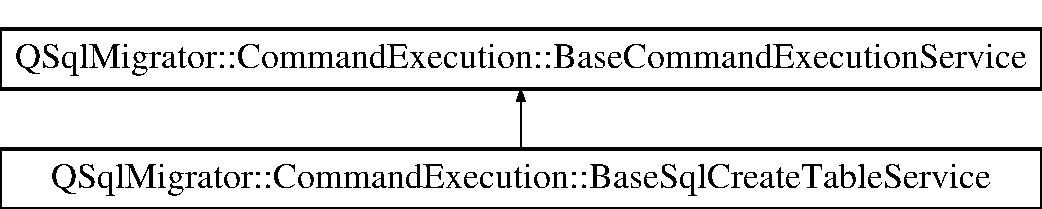
\includegraphics[height=2.000000cm]{class_q_sql_migrator_1_1_command_execution_1_1_base_sql_create_table_service}
\end{center}
\end{figure}
\subsection*{Public Member Functions}
\begin{DoxyCompactItemize}
\item 
\mbox{\Hypertarget{class_q_sql_migrator_1_1_command_execution_1_1_base_sql_create_table_service_aca4697ca0b882d66111f61e2263166c1}\label{class_q_sql_migrator_1_1_command_execution_1_1_base_sql_create_table_service_aca4697ca0b882d66111f61e2263166c1}} 
const Q\+String \& {\bfseries command\+Type} () const
\item 
\mbox{\Hypertarget{class_q_sql_migrator_1_1_command_execution_1_1_base_sql_create_table_service_a13fb173d3ed435cc8892df934f28f2fb}\label{class_q_sql_migrator_1_1_command_execution_1_1_base_sql_create_table_service_a13fb173d3ed435cc8892df934f28f2fb}} 
bool {\bfseries execute} (const Commands\+::\+Const\+Command\+Ptr \&command, \hyperlink{class_q_sql_migrator_1_1_command_execution_1_1_command_execution_context}{Command\+Execution\+::\+Command\+Execution\+Context} \&context) const
\item 
\mbox{\Hypertarget{class_q_sql_migrator_1_1_command_execution_1_1_base_sql_create_table_service_a7abce9c96889171feacb121d960df25e}\label{class_q_sql_migrator_1_1_command_execution_1_1_base_sql_create_table_service_a7abce9c96889171feacb121d960df25e}} 
bool {\bfseries is\+Valid} (const Commands\+::\+Const\+Command\+Ptr \&command, const \hyperlink{class_q_sql_migrator_1_1_command_execution_1_1_command_execution_context}{Command\+Execution\+::\+Command\+Execution\+Context} \&context) const
\end{DoxyCompactItemize}
\subsection*{Static Public Member Functions}
\begin{DoxyCompactItemize}
\item 
\mbox{\Hypertarget{class_q_sql_migrator_1_1_command_execution_1_1_base_sql_create_table_service_adb55f932a6220fbdb587c6570fc88b4a}\label{class_q_sql_migrator_1_1_command_execution_1_1_base_sql_create_table_service_adb55f932a6220fbdb587c6570fc88b4a}} 
static bool {\bfseries execute} (const \hyperlink{class_q_sql_migrator_1_1_commands_1_1_create_table}{Commands\+::\+Create\+Table} \&create\+Table, const \hyperlink{class_q_sql_migrator_1_1_command_execution_1_1_command_execution_context}{Command\+Execution\+::\+Command\+Execution\+Context} \&context)
\end{DoxyCompactItemize}
\subsection*{Additional Inherited Members}


The documentation for this class was generated from the following files\+:\begin{DoxyCompactItemize}
\item 
/home/george/\+Develop/\+Praaline\+Py/praaline-\/core/\+Q\+Sql\+Migrator/\+Base\+Sql\+Migrator/\+Command\+Execution/Base\+Sql\+Create\+Table\+Service.\+h\item 
/home/george/\+Develop/\+Praaline\+Py/praaline-\/core/\+Q\+Sql\+Migrator/\+Base\+Sql\+Migrator/\+Command\+Execution/Base\+Sql\+Create\+Table\+Service.\+cpp\end{DoxyCompactItemize}

\hypertarget{class_q_sql_migrator_1_1_command_execution_1_1_base_sql_drop_column_service}{}\section{Q\+Sql\+Migrator\+:\+:Command\+Execution\+:\+:Base\+Sql\+Drop\+Column\+Service Class Reference}
\label{class_q_sql_migrator_1_1_command_execution_1_1_base_sql_drop_column_service}\index{Q\+Sql\+Migrator\+::\+Command\+Execution\+::\+Base\+Sql\+Drop\+Column\+Service@{Q\+Sql\+Migrator\+::\+Command\+Execution\+::\+Base\+Sql\+Drop\+Column\+Service}}
Inheritance diagram for Q\+Sql\+Migrator\+:\+:Command\+Execution\+:\+:Base\+Sql\+Drop\+Column\+Service\+:\begin{figure}[H]
\begin{center}
\leavevmode
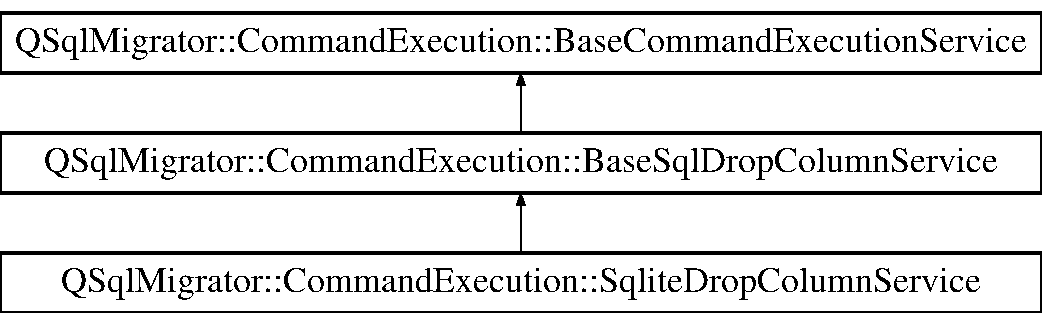
\includegraphics[height=3.000000cm]{class_q_sql_migrator_1_1_command_execution_1_1_base_sql_drop_column_service}
\end{center}
\end{figure}
\subsection*{Public Member Functions}
\begin{DoxyCompactItemize}
\item 
\mbox{\Hypertarget{class_q_sql_migrator_1_1_command_execution_1_1_base_sql_drop_column_service_a33d2a527a1ab1ae8a30af11bfee4c28a}\label{class_q_sql_migrator_1_1_command_execution_1_1_base_sql_drop_column_service_a33d2a527a1ab1ae8a30af11bfee4c28a}} 
const Q\+String \& {\bfseries command\+Type} () const
\item 
\mbox{\Hypertarget{class_q_sql_migrator_1_1_command_execution_1_1_base_sql_drop_column_service_a23b89113a9f772302391405c0ad26bc0}\label{class_q_sql_migrator_1_1_command_execution_1_1_base_sql_drop_column_service_a23b89113a9f772302391405c0ad26bc0}} 
bool {\bfseries execute} (const Commands\+::\+Const\+Command\+Ptr \&command, \hyperlink{class_q_sql_migrator_1_1_command_execution_1_1_command_execution_context}{Command\+Execution\+::\+Command\+Execution\+Context} \&context) const
\item 
\mbox{\Hypertarget{class_q_sql_migrator_1_1_command_execution_1_1_base_sql_drop_column_service_a69976d59f0a4aaaefeee4b74f0056be7}\label{class_q_sql_migrator_1_1_command_execution_1_1_base_sql_drop_column_service_a69976d59f0a4aaaefeee4b74f0056be7}} 
bool {\bfseries is\+Valid} (const Commands\+::\+Const\+Command\+Ptr \&command, const \hyperlink{class_q_sql_migrator_1_1_command_execution_1_1_command_execution_context}{Command\+Execution\+::\+Command\+Execution\+Context} \&context) const
\end{DoxyCompactItemize}
\subsection*{Static Public Member Functions}
\begin{DoxyCompactItemize}
\item 
\mbox{\Hypertarget{class_q_sql_migrator_1_1_command_execution_1_1_base_sql_drop_column_service_ab49258a761b5a2a5f8aef957ba86c653}\label{class_q_sql_migrator_1_1_command_execution_1_1_base_sql_drop_column_service_ab49258a761b5a2a5f8aef957ba86c653}} 
static bool {\bfseries execute} (const \hyperlink{class_q_sql_migrator_1_1_commands_1_1_drop_column}{Commands\+::\+Drop\+Column} \&drop\+Column, const \hyperlink{class_q_sql_migrator_1_1_command_execution_1_1_command_execution_context}{Command\+Execution\+::\+Command\+Execution\+Context} \&context)
\end{DoxyCompactItemize}
\subsection*{Additional Inherited Members}


The documentation for this class was generated from the following files\+:\begin{DoxyCompactItemize}
\item 
/home/george/\+Develop/\+Praaline\+Py/praaline-\/core/\+Q\+Sql\+Migrator/\+Base\+Sql\+Migrator/\+Command\+Execution/Base\+Sql\+Drop\+Column\+Service.\+h\item 
/home/george/\+Develop/\+Praaline\+Py/praaline-\/core/\+Q\+Sql\+Migrator/\+Base\+Sql\+Migrator/\+Command\+Execution/Base\+Sql\+Drop\+Column\+Service.\+cpp\end{DoxyCompactItemize}

\hypertarget{class_q_sql_migrator_1_1_command_execution_1_1_base_sql_drop_index_service}{}\section{Q\+Sql\+Migrator\+:\+:Command\+Execution\+:\+:Base\+Sql\+Drop\+Index\+Service Class Reference}
\label{class_q_sql_migrator_1_1_command_execution_1_1_base_sql_drop_index_service}\index{Q\+Sql\+Migrator\+::\+Command\+Execution\+::\+Base\+Sql\+Drop\+Index\+Service@{Q\+Sql\+Migrator\+::\+Command\+Execution\+::\+Base\+Sql\+Drop\+Index\+Service}}
Inheritance diagram for Q\+Sql\+Migrator\+:\+:Command\+Execution\+:\+:Base\+Sql\+Drop\+Index\+Service\+:\begin{figure}[H]
\begin{center}
\leavevmode
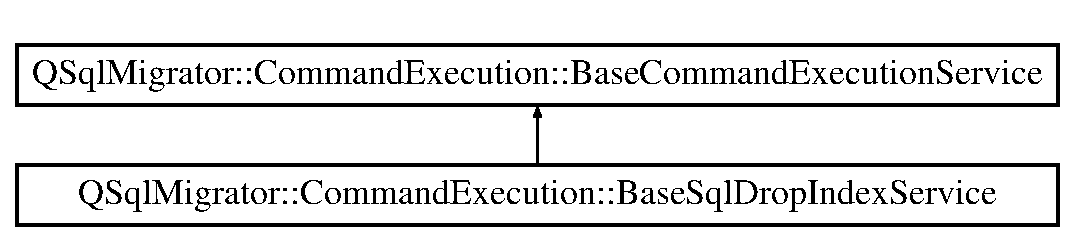
\includegraphics[height=2.000000cm]{class_q_sql_migrator_1_1_command_execution_1_1_base_sql_drop_index_service}
\end{center}
\end{figure}
\subsection*{Public Member Functions}
\begin{DoxyCompactItemize}
\item 
\mbox{\Hypertarget{class_q_sql_migrator_1_1_command_execution_1_1_base_sql_drop_index_service_a208d57d394b2793195621af8d9818659}\label{class_q_sql_migrator_1_1_command_execution_1_1_base_sql_drop_index_service_a208d57d394b2793195621af8d9818659}} 
const Q\+String \& {\bfseries command\+Type} () const
\item 
\mbox{\Hypertarget{class_q_sql_migrator_1_1_command_execution_1_1_base_sql_drop_index_service_a47487ffd6254eaaa5696b5ccf307e4cf}\label{class_q_sql_migrator_1_1_command_execution_1_1_base_sql_drop_index_service_a47487ffd6254eaaa5696b5ccf307e4cf}} 
bool {\bfseries execute} (const Commands\+::\+Const\+Command\+Ptr \&command, \hyperlink{class_q_sql_migrator_1_1_command_execution_1_1_command_execution_context}{Command\+Execution\+::\+Command\+Execution\+Context} \&context) const
\item 
\mbox{\Hypertarget{class_q_sql_migrator_1_1_command_execution_1_1_base_sql_drop_index_service_a729542b61bc3a2f7bb0c55cca39ea6ea}\label{class_q_sql_migrator_1_1_command_execution_1_1_base_sql_drop_index_service_a729542b61bc3a2f7bb0c55cca39ea6ea}} 
bool {\bfseries is\+Valid} (const Commands\+::\+Const\+Command\+Ptr \&command, const \hyperlink{class_q_sql_migrator_1_1_command_execution_1_1_command_execution_context}{Command\+Execution\+::\+Command\+Execution\+Context} \&context) const
\end{DoxyCompactItemize}
\subsection*{Static Public Member Functions}
\begin{DoxyCompactItemize}
\item 
\mbox{\Hypertarget{class_q_sql_migrator_1_1_command_execution_1_1_base_sql_drop_index_service_ae18a63b0b2c88794de6a32013fb76b58}\label{class_q_sql_migrator_1_1_command_execution_1_1_base_sql_drop_index_service_ae18a63b0b2c88794de6a32013fb76b58}} 
static bool {\bfseries execute} (const \hyperlink{class_q_sql_migrator_1_1_commands_1_1_drop_index}{Commands\+::\+Drop\+Index} \&drop\+Index, const \hyperlink{class_q_sql_migrator_1_1_command_execution_1_1_command_execution_context}{Command\+Execution\+::\+Command\+Execution\+Context} \&context)
\end{DoxyCompactItemize}
\subsection*{Additional Inherited Members}


The documentation for this class was generated from the following files\+:\begin{DoxyCompactItemize}
\item 
/home/george/\+Develop/\+Praaline\+Py/praaline-\/core/\+Q\+Sql\+Migrator/\+Base\+Sql\+Migrator/\+Command\+Execution/Base\+Sql\+Drop\+Index\+Service.\+h\item 
/home/george/\+Develop/\+Praaline\+Py/praaline-\/core/\+Q\+Sql\+Migrator/\+Base\+Sql\+Migrator/\+Command\+Execution/Base\+Sql\+Drop\+Index\+Service.\+cpp\end{DoxyCompactItemize}

\hypertarget{class_q_sql_migrator_1_1_command_execution_1_1_base_sql_drop_table_service}{}\section{Q\+Sql\+Migrator\+:\+:Command\+Execution\+:\+:Base\+Sql\+Drop\+Table\+Service Class Reference}
\label{class_q_sql_migrator_1_1_command_execution_1_1_base_sql_drop_table_service}\index{Q\+Sql\+Migrator\+::\+Command\+Execution\+::\+Base\+Sql\+Drop\+Table\+Service@{Q\+Sql\+Migrator\+::\+Command\+Execution\+::\+Base\+Sql\+Drop\+Table\+Service}}
Inheritance diagram for Q\+Sql\+Migrator\+:\+:Command\+Execution\+:\+:Base\+Sql\+Drop\+Table\+Service\+:\begin{figure}[H]
\begin{center}
\leavevmode
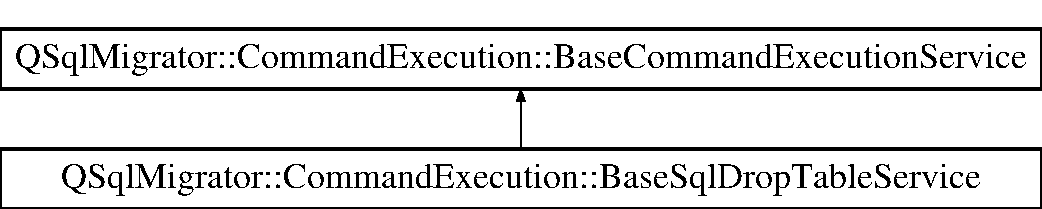
\includegraphics[height=2.000000cm]{class_q_sql_migrator_1_1_command_execution_1_1_base_sql_drop_table_service}
\end{center}
\end{figure}
\subsection*{Public Member Functions}
\begin{DoxyCompactItemize}
\item 
\mbox{\Hypertarget{class_q_sql_migrator_1_1_command_execution_1_1_base_sql_drop_table_service_aa9688ed5f8b080e834f4d7e8e04e8174}\label{class_q_sql_migrator_1_1_command_execution_1_1_base_sql_drop_table_service_aa9688ed5f8b080e834f4d7e8e04e8174}} 
const Q\+String \& {\bfseries command\+Type} () const
\item 
\mbox{\Hypertarget{class_q_sql_migrator_1_1_command_execution_1_1_base_sql_drop_table_service_a6ee61337743cf5bc05a4898af872b6e7}\label{class_q_sql_migrator_1_1_command_execution_1_1_base_sql_drop_table_service_a6ee61337743cf5bc05a4898af872b6e7}} 
bool {\bfseries execute} (const Commands\+::\+Const\+Command\+Ptr \&command, \hyperlink{class_q_sql_migrator_1_1_command_execution_1_1_command_execution_context}{Command\+Execution\+::\+Command\+Execution\+Context} \&context) const
\item 
\mbox{\Hypertarget{class_q_sql_migrator_1_1_command_execution_1_1_base_sql_drop_table_service_a74e154fabd0fe41c62c8cd9b34b4197a}\label{class_q_sql_migrator_1_1_command_execution_1_1_base_sql_drop_table_service_a74e154fabd0fe41c62c8cd9b34b4197a}} 
bool {\bfseries is\+Valid} (const Commands\+::\+Const\+Command\+Ptr \&command, const \hyperlink{class_q_sql_migrator_1_1_command_execution_1_1_command_execution_context}{Command\+Execution\+::\+Command\+Execution\+Context} \&context) const
\end{DoxyCompactItemize}
\subsection*{Static Public Member Functions}
\begin{DoxyCompactItemize}
\item 
\mbox{\Hypertarget{class_q_sql_migrator_1_1_command_execution_1_1_base_sql_drop_table_service_a8e48525f31a24f959cb38bfa612ab65b}\label{class_q_sql_migrator_1_1_command_execution_1_1_base_sql_drop_table_service_a8e48525f31a24f959cb38bfa612ab65b}} 
static bool {\bfseries execute} (const \hyperlink{class_q_sql_migrator_1_1_commands_1_1_drop_table}{Commands\+::\+Drop\+Table} \&drop\+Table, const \hyperlink{class_q_sql_migrator_1_1_command_execution_1_1_command_execution_context}{Command\+Execution\+::\+Command\+Execution\+Context} \&context)
\end{DoxyCompactItemize}
\subsection*{Additional Inherited Members}


The documentation for this class was generated from the following files\+:\begin{DoxyCompactItemize}
\item 
/home/george/\+Develop/\+Praaline\+Py/praaline-\/core/\+Q\+Sql\+Migrator/\+Base\+Sql\+Migrator/\+Command\+Execution/Base\+Sql\+Drop\+Table\+Service.\+h\item 
/home/george/\+Develop/\+Praaline\+Py/praaline-\/core/\+Q\+Sql\+Migrator/\+Base\+Sql\+Migrator/\+Command\+Execution/Base\+Sql\+Drop\+Table\+Service.\+cpp\end{DoxyCompactItemize}

\hypertarget{class_q_sql_migrator_1_1_helper_1_1_base_sql_quote_service}{}\section{Q\+Sql\+Migrator\+:\+:Helper\+:\+:Base\+Sql\+Quote\+Service Class Reference}
\label{class_q_sql_migrator_1_1_helper_1_1_base_sql_quote_service}\index{Q\+Sql\+Migrator\+::\+Helper\+::\+Base\+Sql\+Quote\+Service@{Q\+Sql\+Migrator\+::\+Helper\+::\+Base\+Sql\+Quote\+Service}}
Inheritance diagram for Q\+Sql\+Migrator\+:\+:Helper\+:\+:Base\+Sql\+Quote\+Service\+:\begin{figure}[H]
\begin{center}
\leavevmode
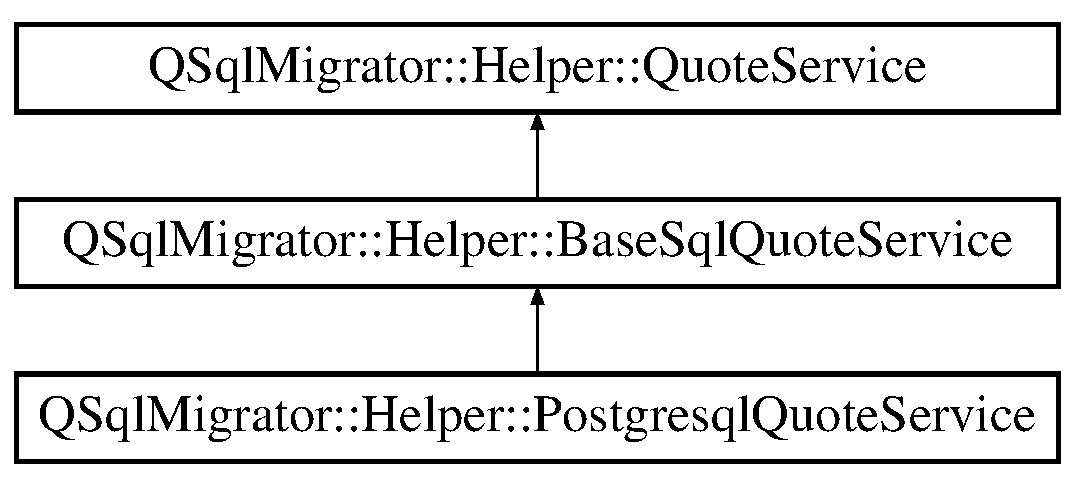
\includegraphics[height=3.000000cm]{class_q_sql_migrator_1_1_helper_1_1_base_sql_quote_service}
\end{center}
\end{figure}
\subsection*{Public Member Functions}
\begin{DoxyCompactItemize}
\item 
Q\+String \hyperlink{class_q_sql_migrator_1_1_helper_1_1_base_sql_quote_service_aacd2ed13fd6f57bc77b4870ac5105f9e}{quote\+Table\+Name} (const Q\+String \&table\+Name) const Q\+\_\+\+D\+E\+C\+L\+\_\+\+O\+V\+E\+R\+R\+I\+DE
\item 
Q\+String \hyperlink{class_q_sql_migrator_1_1_helper_1_1_base_sql_quote_service_a26aebafe6d736520b5661c82a4db4ae9}{quote\+Column\+Name} (const Q\+String \&column\+Name) const Q\+\_\+\+D\+E\+C\+L\+\_\+\+O\+V\+E\+R\+R\+I\+DE
\item 
Q\+String \hyperlink{class_q_sql_migrator_1_1_helper_1_1_base_sql_quote_service_a54146919b3027be887151bcc27c56dad}{quote\+String} (const Q\+String \&string) const Q\+\_\+\+D\+E\+C\+L\+\_\+\+O\+V\+E\+R\+R\+I\+DE
\end{DoxyCompactItemize}


\subsection{Member Function Documentation}
\mbox{\Hypertarget{class_q_sql_migrator_1_1_helper_1_1_base_sql_quote_service_a26aebafe6d736520b5661c82a4db4ae9}\label{class_q_sql_migrator_1_1_helper_1_1_base_sql_quote_service_a26aebafe6d736520b5661c82a4db4ae9}} 
\index{Q\+Sql\+Migrator\+::\+Helper\+::\+Base\+Sql\+Quote\+Service@{Q\+Sql\+Migrator\+::\+Helper\+::\+Base\+Sql\+Quote\+Service}!quote\+Column\+Name@{quote\+Column\+Name}}
\index{quote\+Column\+Name@{quote\+Column\+Name}!Q\+Sql\+Migrator\+::\+Helper\+::\+Base\+Sql\+Quote\+Service@{Q\+Sql\+Migrator\+::\+Helper\+::\+Base\+Sql\+Quote\+Service}}
\subsubsection{\texorpdfstring{quote\+Column\+Name()}{quoteColumnName()}}
{\footnotesize\ttfamily Q\+String Q\+Sql\+Migrator\+::\+Helper\+::\+Base\+Sql\+Quote\+Service\+::quote\+Column\+Name (\begin{DoxyParamCaption}\item[{const Q\+String \&}]{column\+Name }\end{DoxyParamCaption}) const\hspace{0.3cm}{\ttfamily [virtual]}}

\begin{DoxyReturn}{Returns}
the column name properly quoted for an sql execution 
\end{DoxyReturn}


Implements \hyperlink{class_q_sql_migrator_1_1_helper_1_1_quote_service_ae5ed3750bb00609d483996e7baa6f885}{Q\+Sql\+Migrator\+::\+Helper\+::\+Quote\+Service}.



Reimplemented in \hyperlink{class_q_sql_migrator_1_1_helper_1_1_postgresql_quote_service_af54cb8f1749e470e2ea8794fb58896c8}{Q\+Sql\+Migrator\+::\+Helper\+::\+Postgresql\+Quote\+Service}.

\mbox{\Hypertarget{class_q_sql_migrator_1_1_helper_1_1_base_sql_quote_service_a54146919b3027be887151bcc27c56dad}\label{class_q_sql_migrator_1_1_helper_1_1_base_sql_quote_service_a54146919b3027be887151bcc27c56dad}} 
\index{Q\+Sql\+Migrator\+::\+Helper\+::\+Base\+Sql\+Quote\+Service@{Q\+Sql\+Migrator\+::\+Helper\+::\+Base\+Sql\+Quote\+Service}!quote\+String@{quote\+String}}
\index{quote\+String@{quote\+String}!Q\+Sql\+Migrator\+::\+Helper\+::\+Base\+Sql\+Quote\+Service@{Q\+Sql\+Migrator\+::\+Helper\+::\+Base\+Sql\+Quote\+Service}}
\subsubsection{\texorpdfstring{quote\+String()}{quoteString()}}
{\footnotesize\ttfamily Q\+String Q\+Sql\+Migrator\+::\+Helper\+::\+Base\+Sql\+Quote\+Service\+::quote\+String (\begin{DoxyParamCaption}\item[{const Q\+String \&}]{string }\end{DoxyParamCaption}) const\hspace{0.3cm}{\ttfamily [virtual]}}

\begin{DoxyReturn}{Returns}
the string value properly quoted for an sql execution 
\end{DoxyReturn}


Implements \hyperlink{class_q_sql_migrator_1_1_helper_1_1_quote_service_a5a557ef5b418afcbe9ae01ce57616218}{Q\+Sql\+Migrator\+::\+Helper\+::\+Quote\+Service}.



Reimplemented in \hyperlink{class_q_sql_migrator_1_1_helper_1_1_postgresql_quote_service_aea4456a2d9ae05fbc1bb653dfcb6571f}{Q\+Sql\+Migrator\+::\+Helper\+::\+Postgresql\+Quote\+Service}.

\mbox{\Hypertarget{class_q_sql_migrator_1_1_helper_1_1_base_sql_quote_service_aacd2ed13fd6f57bc77b4870ac5105f9e}\label{class_q_sql_migrator_1_1_helper_1_1_base_sql_quote_service_aacd2ed13fd6f57bc77b4870ac5105f9e}} 
\index{Q\+Sql\+Migrator\+::\+Helper\+::\+Base\+Sql\+Quote\+Service@{Q\+Sql\+Migrator\+::\+Helper\+::\+Base\+Sql\+Quote\+Service}!quote\+Table\+Name@{quote\+Table\+Name}}
\index{quote\+Table\+Name@{quote\+Table\+Name}!Q\+Sql\+Migrator\+::\+Helper\+::\+Base\+Sql\+Quote\+Service@{Q\+Sql\+Migrator\+::\+Helper\+::\+Base\+Sql\+Quote\+Service}}
\subsubsection{\texorpdfstring{quote\+Table\+Name()}{quoteTableName()}}
{\footnotesize\ttfamily Q\+String Q\+Sql\+Migrator\+::\+Helper\+::\+Base\+Sql\+Quote\+Service\+::quote\+Table\+Name (\begin{DoxyParamCaption}\item[{const Q\+String \&}]{table\+Name }\end{DoxyParamCaption}) const\hspace{0.3cm}{\ttfamily [virtual]}}

\begin{DoxyReturn}{Returns}
the table name properly quoted for an sql execution 
\end{DoxyReturn}


Implements \hyperlink{class_q_sql_migrator_1_1_helper_1_1_quote_service_acb56728a4d07a8857955e34536844ec7}{Q\+Sql\+Migrator\+::\+Helper\+::\+Quote\+Service}.



Reimplemented in \hyperlink{class_q_sql_migrator_1_1_helper_1_1_postgresql_quote_service_a56541b2bbc99faae890a9a21d50e14f6}{Q\+Sql\+Migrator\+::\+Helper\+::\+Postgresql\+Quote\+Service}.



The documentation for this class was generated from the following files\+:\begin{DoxyCompactItemize}
\item 
/home/george/\+Develop/\+Praaline\+Py/praaline-\/core/\+Q\+Sql\+Migrator/\+Base\+Sql\+Migrator/\+Helper/Base\+Sql\+Quote\+Service.\+h\item 
/home/george/\+Develop/\+Praaline\+Py/praaline-\/core/\+Q\+Sql\+Migrator/\+Base\+Sql\+Migrator/\+Helper/Base\+Sql\+Quote\+Service.\+cpp\end{DoxyCompactItemize}

\hypertarget{class_q_sql_migrator_1_1_command_execution_1_1_base_sql_rename_column_service}{}\section{Q\+Sql\+Migrator\+:\+:Command\+Execution\+:\+:Base\+Sql\+Rename\+Column\+Service Class Reference}
\label{class_q_sql_migrator_1_1_command_execution_1_1_base_sql_rename_column_service}\index{Q\+Sql\+Migrator\+::\+Command\+Execution\+::\+Base\+Sql\+Rename\+Column\+Service@{Q\+Sql\+Migrator\+::\+Command\+Execution\+::\+Base\+Sql\+Rename\+Column\+Service}}
Inheritance diagram for Q\+Sql\+Migrator\+:\+:Command\+Execution\+:\+:Base\+Sql\+Rename\+Column\+Service\+:\begin{figure}[H]
\begin{center}
\leavevmode
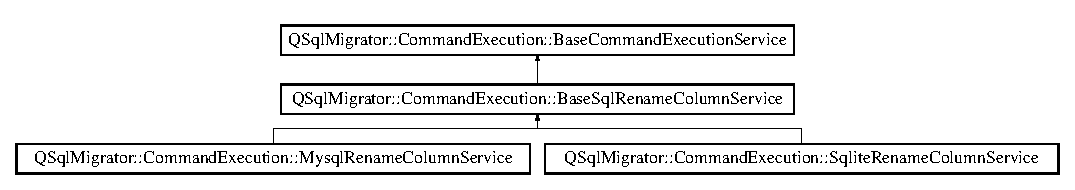
\includegraphics[height=2.105263cm]{class_q_sql_migrator_1_1_command_execution_1_1_base_sql_rename_column_service}
\end{center}
\end{figure}
\subsection*{Public Member Functions}
\begin{DoxyCompactItemize}
\item 
\mbox{\Hypertarget{class_q_sql_migrator_1_1_command_execution_1_1_base_sql_rename_column_service_a0730bd4569b311e6a0bf3f141e28dac5}\label{class_q_sql_migrator_1_1_command_execution_1_1_base_sql_rename_column_service_a0730bd4569b311e6a0bf3f141e28dac5}} 
const Q\+String \& {\bfseries command\+Type} () const
\item 
\mbox{\Hypertarget{class_q_sql_migrator_1_1_command_execution_1_1_base_sql_rename_column_service_ae56b771f42a573520402c232e4238985}\label{class_q_sql_migrator_1_1_command_execution_1_1_base_sql_rename_column_service_ae56b771f42a573520402c232e4238985}} 
bool {\bfseries execute} (const Commands\+::\+Const\+Command\+Ptr \&command, \hyperlink{class_q_sql_migrator_1_1_command_execution_1_1_command_execution_context}{Command\+Execution\+::\+Command\+Execution\+Context} \&context) const
\item 
\mbox{\Hypertarget{class_q_sql_migrator_1_1_command_execution_1_1_base_sql_rename_column_service_af585a49b13bc0a1a4b164d0fd37a6797}\label{class_q_sql_migrator_1_1_command_execution_1_1_base_sql_rename_column_service_af585a49b13bc0a1a4b164d0fd37a6797}} 
bool {\bfseries is\+Valid} (const Commands\+::\+Const\+Command\+Ptr \&command, const \hyperlink{class_q_sql_migrator_1_1_command_execution_1_1_command_execution_context}{Command\+Execution\+::\+Command\+Execution\+Context} \&context) const
\end{DoxyCompactItemize}
\subsection*{Static Public Member Functions}
\begin{DoxyCompactItemize}
\item 
\mbox{\Hypertarget{class_q_sql_migrator_1_1_command_execution_1_1_base_sql_rename_column_service_a96607217501c92369a3ef83651ab0918}\label{class_q_sql_migrator_1_1_command_execution_1_1_base_sql_rename_column_service_a96607217501c92369a3ef83651ab0918}} 
static bool {\bfseries execute} (const \hyperlink{class_q_sql_migrator_1_1_commands_1_1_rename_column}{Commands\+::\+Rename\+Column} \&rename\+Column, const \hyperlink{class_q_sql_migrator_1_1_command_execution_1_1_command_execution_context}{Command\+Execution\+::\+Command\+Execution\+Context} \&context)
\end{DoxyCompactItemize}
\subsection*{Additional Inherited Members}


The documentation for this class was generated from the following files\+:\begin{DoxyCompactItemize}
\item 
/home/george/\+Develop/\+Praaline\+Py/praaline-\/core/\+Q\+Sql\+Migrator/\+Base\+Sql\+Migrator/\+Command\+Execution/Base\+Sql\+Rename\+Column\+Service.\+h\item 
/home/george/\+Develop/\+Praaline\+Py/praaline-\/core/\+Q\+Sql\+Migrator/\+Base\+Sql\+Migrator/\+Command\+Execution/Base\+Sql\+Rename\+Column\+Service.\+cpp\end{DoxyCompactItemize}

\hypertarget{class_q_sql_migrator_1_1_command_execution_1_1_base_sql_rename_table_service}{}\section{Q\+Sql\+Migrator\+:\+:Command\+Execution\+:\+:Base\+Sql\+Rename\+Table\+Service Class Reference}
\label{class_q_sql_migrator_1_1_command_execution_1_1_base_sql_rename_table_service}\index{Q\+Sql\+Migrator\+::\+Command\+Execution\+::\+Base\+Sql\+Rename\+Table\+Service@{Q\+Sql\+Migrator\+::\+Command\+Execution\+::\+Base\+Sql\+Rename\+Table\+Service}}
Inheritance diagram for Q\+Sql\+Migrator\+:\+:Command\+Execution\+:\+:Base\+Sql\+Rename\+Table\+Service\+:\begin{figure}[H]
\begin{center}
\leavevmode
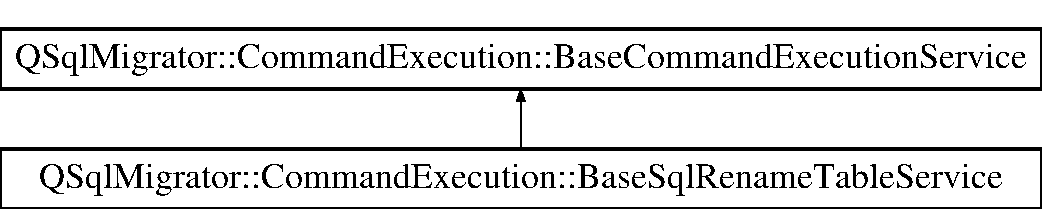
\includegraphics[height=2.000000cm]{class_q_sql_migrator_1_1_command_execution_1_1_base_sql_rename_table_service}
\end{center}
\end{figure}
\subsection*{Public Member Functions}
\begin{DoxyCompactItemize}
\item 
\mbox{\Hypertarget{class_q_sql_migrator_1_1_command_execution_1_1_base_sql_rename_table_service_a28a6819635774c94918b66cde14d0be8}\label{class_q_sql_migrator_1_1_command_execution_1_1_base_sql_rename_table_service_a28a6819635774c94918b66cde14d0be8}} 
const Q\+String \& {\bfseries command\+Type} () const
\item 
\mbox{\Hypertarget{class_q_sql_migrator_1_1_command_execution_1_1_base_sql_rename_table_service_adf78e320b70ceb6e2ee8f37d31bbe2cd}\label{class_q_sql_migrator_1_1_command_execution_1_1_base_sql_rename_table_service_adf78e320b70ceb6e2ee8f37d31bbe2cd}} 
bool {\bfseries execute} (const Commands\+::\+Const\+Command\+Ptr \&command, \hyperlink{class_q_sql_migrator_1_1_command_execution_1_1_command_execution_context}{Command\+Execution\+::\+Command\+Execution\+Context} \&context) const
\item 
\mbox{\Hypertarget{class_q_sql_migrator_1_1_command_execution_1_1_base_sql_rename_table_service_af8ac85be5575eb1c0e7fdd6f3f068852}\label{class_q_sql_migrator_1_1_command_execution_1_1_base_sql_rename_table_service_af8ac85be5575eb1c0e7fdd6f3f068852}} 
bool {\bfseries is\+Valid} (const Commands\+::\+Const\+Command\+Ptr \&command, const \hyperlink{class_q_sql_migrator_1_1_command_execution_1_1_command_execution_context}{Command\+Execution\+::\+Command\+Execution\+Context} \&context) const
\end{DoxyCompactItemize}
\subsection*{Static Public Member Functions}
\begin{DoxyCompactItemize}
\item 
\mbox{\Hypertarget{class_q_sql_migrator_1_1_command_execution_1_1_base_sql_rename_table_service_ab68c97ce6abd3d05b3a208219264d225}\label{class_q_sql_migrator_1_1_command_execution_1_1_base_sql_rename_table_service_ab68c97ce6abd3d05b3a208219264d225}} 
static bool {\bfseries execute} (const \hyperlink{class_q_sql_migrator_1_1_commands_1_1_rename_table}{Commands\+::\+Rename\+Table} \&rename\+Table, const \hyperlink{class_q_sql_migrator_1_1_command_execution_1_1_command_execution_context}{Command\+Execution\+Context} \&context)
\end{DoxyCompactItemize}
\subsection*{Additional Inherited Members}


The documentation for this class was generated from the following files\+:\begin{DoxyCompactItemize}
\item 
/home/george/\+Develop/\+Praaline\+Py/praaline-\/core/\+Q\+Sql\+Migrator/\+Base\+Sql\+Migrator/\+Command\+Execution/Base\+Sql\+Rename\+Table\+Service.\+h\item 
/home/george/\+Develop/\+Praaline\+Py/praaline-\/core/\+Q\+Sql\+Migrator/\+Base\+Sql\+Migrator/\+Command\+Execution/Base\+Sql\+Rename\+Table\+Service.\+cpp\end{DoxyCompactItemize}

\hypertarget{class_q_sql_migrator_1_1_helper_1_1_base_sql_type_mapper_service}{}\section{Q\+Sql\+Migrator\+:\+:Helper\+:\+:Base\+Sql\+Type\+Mapper\+Service Class Reference}
\label{class_q_sql_migrator_1_1_helper_1_1_base_sql_type_mapper_service}\index{Q\+Sql\+Migrator\+::\+Helper\+::\+Base\+Sql\+Type\+Mapper\+Service@{Q\+Sql\+Migrator\+::\+Helper\+::\+Base\+Sql\+Type\+Mapper\+Service}}


standard sql type mapping implementation  




{\ttfamily \#include $<$Base\+Sql\+Type\+Mapper\+Service.\+h$>$}

Inheritance diagram for Q\+Sql\+Migrator\+:\+:Helper\+:\+:Base\+Sql\+Type\+Mapper\+Service\+:\begin{figure}[H]
\begin{center}
\leavevmode
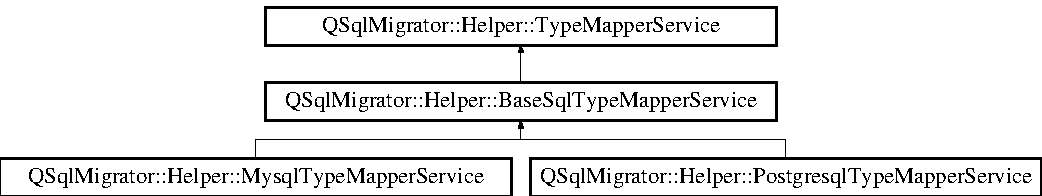
\includegraphics[height=2.633229cm]{class_q_sql_migrator_1_1_helper_1_1_base_sql_type_mapper_service}
\end{center}
\end{figure}
\subsection*{Public Member Functions}
\begin{DoxyCompactItemize}
\item 
\mbox{\Hypertarget{class_q_sql_migrator_1_1_helper_1_1_base_sql_type_mapper_service_a0fe8a469f062155edb1199e1c4e742d8}\label{class_q_sql_migrator_1_1_helper_1_1_base_sql_type_mapper_service_a0fe8a469f062155edb1199e1c4e742d8}} 
Q\+String {\bfseries map} (const \hyperlink{class_q_sql_migrator_1_1_structure_1_1_sql_type}{Structure\+::\+Sql\+Type} \&type) const Q\+\_\+\+D\+E\+C\+L\+\_\+\+O\+V\+E\+R\+R\+I\+DE
\end{DoxyCompactItemize}
\subsection*{Protected Attributes}
\begin{DoxyCompactItemize}
\item 
\mbox{\Hypertarget{class_q_sql_migrator_1_1_helper_1_1_base_sql_type_mapper_service_a0896a6b1fca59b9075ba6cab5bbf4ec5}\label{class_q_sql_migrator_1_1_helper_1_1_base_sql_type_mapper_service_a0896a6b1fca59b9075ba6cab5bbf4ec5}} 
Q\+Hash$<$ \hyperlink{class_q_sql_migrator_1_1_structure_1_1_sql_type_ac1733fcbed79941acd89bcf3196d9912}{Structure\+::\+Sql\+Type\+::\+Base}, Q\+String $>$ {\bfseries m\+\_\+type\+Map}
\end{DoxyCompactItemize}


\subsection{Detailed Description}
standard sql type mapping implementation 

The documentation for this class was generated from the following files\+:\begin{DoxyCompactItemize}
\item 
/home/george/\+Develop/\+Praaline\+Py/praaline-\/core/\+Q\+Sql\+Migrator/\+Base\+Sql\+Migrator/\+Helper/Base\+Sql\+Type\+Mapper\+Service.\+h\item 
/home/george/\+Develop/\+Praaline\+Py/praaline-\/core/\+Q\+Sql\+Migrator/\+Base\+Sql\+Migrator/\+Helper/Base\+Sql\+Type\+Mapper\+Service.\+cpp\end{DoxyCompactItemize}

\hypertarget{class_q_sql_migrator_1_1_migration_execution_1_1_migration_execution_context_1_1_builder}{}\section{Q\+Sql\+Migrator\+:\+:Migration\+Execution\+:\+:Migration\+Execution\+Context\+:\+:Builder Class Reference}
\label{class_q_sql_migrator_1_1_migration_execution_1_1_migration_execution_context_1_1_builder}\index{Q\+Sql\+Migrator\+::\+Migration\+Execution\+::\+Migration\+Execution\+Context\+::\+Builder@{Q\+Sql\+Migrator\+::\+Migration\+Execution\+::\+Migration\+Execution\+Context\+::\+Builder}}
\subsection*{Public Member Functions}
\begin{DoxyCompactItemize}
\item 
\mbox{\Hypertarget{class_q_sql_migrator_1_1_migration_execution_1_1_migration_execution_context_1_1_builder_a3d9c98a9de313a99cff64abf47563933}\label{class_q_sql_migrator_1_1_migration_execution_1_1_migration_execution_context_1_1_builder_a3d9c98a9de313a99cff64abf47563933}} 
{\bfseries Builder} (const Name\+Migration\+Map \&migrations)
\item 
\mbox{\Hypertarget{class_q_sql_migrator_1_1_migration_execution_1_1_migration_execution_context_1_1_builder_ace2423710b55d240f4df28f6d60dd553}\label{class_q_sql_migrator_1_1_migration_execution_1_1_migration_execution_context_1_1_builder_ace2423710b55d240f4df28f6d60dd553}} 
void {\bfseries set\+Config} (const \hyperlink{struct_q_sql_migrator_1_1_migration_execution_1_1_migration_execution_config}{Migration\+Execution\+Config} \&migration\+Config)
\item 
\mbox{\Hypertarget{class_q_sql_migrator_1_1_migration_execution_1_1_migration_execution_context_1_1_builder_a51ba03a0a9b7d7dc3b8936c9e7823cd3}\label{class_q_sql_migrator_1_1_migration_execution_1_1_migration_execution_context_1_1_builder_a51ba03a0a9b7d7dc3b8936c9e7823cd3}} 
void {\bfseries set\+Database} (const Q\+Sql\+Database \&database)
\item 
\mbox{\Hypertarget{class_q_sql_migrator_1_1_migration_execution_1_1_migration_execution_context_1_1_builder_a642e75548a8d71b1459e4964a36e0fe6}\label{class_q_sql_migrator_1_1_migration_execution_1_1_migration_execution_context_1_1_builder_a642e75548a8d71b1459e4964a36e0fe6}} 
Migration\+Execution\+Context\+Ptr {\bfseries build} (const Command\+Service\+Repository\+Ptr \&command\+Service\+Repository, const \hyperlink{class_q_sql_migrator_1_1_helper_1_1_helper_repository}{Helper\+::\+Helper\+Repository} \&helper\+Repository, const Migration\+Table\+Service\+Ptr \&migration\+Table\+Service) const
\end{DoxyCompactItemize}


The documentation for this class was generated from the following files\+:\begin{DoxyCompactItemize}
\item 
/home/george/\+Develop/\+Praaline\+Py/praaline-\/core/\+Q\+Sql\+Migrator/\+Migration\+Execution/Migration\+Execution\+Context.\+h\item 
/home/george/\+Develop/\+Praaline\+Py/praaline-\/core/\+Q\+Sql\+Migrator/\+Migration\+Execution/Migration\+Execution\+Context.\+cpp\end{DoxyCompactItemize}

\hypertarget{class_q_sql_migrator_1_1_structure_1_1_index_1_1_builder}{}\section{Q\+Sql\+Migrator\+:\+:Structure\+:\+:Index\+:\+:Builder Class Reference}
\label{class_q_sql_migrator_1_1_structure_1_1_index_1_1_builder}\index{Q\+Sql\+Migrator\+::\+Structure\+::\+Index\+::\+Builder@{Q\+Sql\+Migrator\+::\+Structure\+::\+Index\+::\+Builder}}


helper to build \hyperlink{class_q_sql_migrator_1_1_structure_1_1_index}{Index} classes  




{\ttfamily \#include $<$Index.\+h$>$}

\subsection*{Public Member Functions}
\begin{DoxyCompactItemize}
\item 
\mbox{\Hypertarget{class_q_sql_migrator_1_1_structure_1_1_index_1_1_builder_a5ccd0c7b5fac4fe4a4b717fa0d54f7af}\label{class_q_sql_migrator_1_1_structure_1_1_index_1_1_builder_a5ccd0c7b5fac4fe4a4b717fa0d54f7af}} 
{\bfseries Builder} (const Q\+String \&name, const Q\+String \&table\+Name)
\item 
\mbox{\Hypertarget{class_q_sql_migrator_1_1_structure_1_1_index_1_1_builder_a00103e732bf6cd77e1f55c2d44bb45f8}\label{class_q_sql_migrator_1_1_structure_1_1_index_1_1_builder_a00103e732bf6cd77e1f55c2d44bb45f8}} 
{\bfseries Builder} (const Q\+String \&name)
\item 
\mbox{\Hypertarget{class_q_sql_migrator_1_1_structure_1_1_index_1_1_builder_abc9757fbefe78fff24012940723c955f}\label{class_q_sql_migrator_1_1_structure_1_1_index_1_1_builder_abc9757fbefe78fff24012940723c955f}} 
\hyperlink{class_q_sql_migrator_1_1_structure_1_1_index_1_1_builder}{Builder} \& {\bfseries operator$<$$<$} (const \hyperlink{class_q_sql_migrator_1_1_structure_1_1_index_1_1_column}{Index\+::\+Column} \&column)
\item 
\mbox{\Hypertarget{class_q_sql_migrator_1_1_structure_1_1_index_1_1_builder_a50a86c052de4261f03649692af2e6104}\label{class_q_sql_migrator_1_1_structure_1_1_index_1_1_builder_a50a86c052de4261f03649692af2e6104}} 
{\bfseries operator Index} () const
\end{DoxyCompactItemize}


\subsection{Detailed Description}
helper to build \hyperlink{class_q_sql_migrator_1_1_structure_1_1_index}{Index} classes 

The documentation for this class was generated from the following files\+:\begin{DoxyCompactItemize}
\item 
/home/george/\+Develop/\+Praaline\+Py/praaline-\/core/\+Q\+Sql\+Migrator/\+Structure/Index.\+h\item 
/home/george/\+Develop/\+Praaline\+Py/praaline-\/core/\+Q\+Sql\+Migrator/\+Structure/Index.\+cpp\end{DoxyCompactItemize}

\hypertarget{class_q_sql_migrator_1_1_structure_1_1_table_1_1_builder}{}\section{Q\+Sql\+Migrator\+:\+:Structure\+:\+:Table\+:\+:Builder Class Reference}
\label{class_q_sql_migrator_1_1_structure_1_1_table_1_1_builder}\index{Q\+Sql\+Migrator\+::\+Structure\+::\+Table\+::\+Builder@{Q\+Sql\+Migrator\+::\+Structure\+::\+Table\+::\+Builder}}
\subsection*{Public Member Functions}
\begin{DoxyCompactItemize}
\item 
\mbox{\Hypertarget{class_q_sql_migrator_1_1_structure_1_1_table_1_1_builder_a39eac2b75ff6a49ee98de58e89fdde18}\label{class_q_sql_migrator_1_1_structure_1_1_table_1_1_builder_a39eac2b75ff6a49ee98de58e89fdde18}} 
{\bfseries Builder} (const Q\+String \&name, const Column\+List \&columns)
\item 
\mbox{\Hypertarget{class_q_sql_migrator_1_1_structure_1_1_table_1_1_builder_ab83907e8f11875c5109cff0faa71e57a}\label{class_q_sql_migrator_1_1_structure_1_1_table_1_1_builder_ab83907e8f11875c5109cff0faa71e57a}} 
{\bfseries Builder} (const Q\+String \&name)
\item 
\mbox{\Hypertarget{class_q_sql_migrator_1_1_structure_1_1_table_1_1_builder_a036741faad713fb6c88984682ea2f42f}\label{class_q_sql_migrator_1_1_structure_1_1_table_1_1_builder_a036741faad713fb6c88984682ea2f42f}} 
\hyperlink{class_q_sql_migrator_1_1_structure_1_1_table_1_1_builder}{Builder} \& {\bfseries operator$<$$<$} (const \hyperlink{class_q_sql_migrator_1_1_structure_1_1_column}{Column} \&column)
\item 
\mbox{\Hypertarget{class_q_sql_migrator_1_1_structure_1_1_table_1_1_builder_a25d424810dc95bf775961c129dd6a15a}\label{class_q_sql_migrator_1_1_structure_1_1_table_1_1_builder_a25d424810dc95bf775961c129dd6a15a}} 
{\bfseries operator Table} ()
\end{DoxyCompactItemize}


The documentation for this class was generated from the following files\+:\begin{DoxyCompactItemize}
\item 
/home/george/\+Develop/\+Praaline\+Py/praaline-\/core/\+Q\+Sql\+Migrator/\+Structure/Table.\+h\item 
/home/george/\+Develop/\+Praaline\+Py/praaline-\/core/\+Q\+Sql\+Migrator/\+Structure/Table.\+cpp\end{DoxyCompactItemize}

\hypertarget{class_q_sql_migrator_1_1_structure_1_1_index_1_1_column}{}\section{Q\+Sql\+Migrator\+:\+:Structure\+:\+:Index\+:\+:Column Class Reference}
\label{class_q_sql_migrator_1_1_structure_1_1_index_1_1_column}\index{Q\+Sql\+Migrator\+::\+Structure\+::\+Index\+::\+Column@{Q\+Sql\+Migrator\+::\+Structure\+::\+Index\+::\+Column}}


index column reference  




{\ttfamily \#include $<$Index.\+h$>$}

\subsection*{Public Member Functions}
\begin{DoxyCompactItemize}
\item 
\mbox{\Hypertarget{class_q_sql_migrator_1_1_structure_1_1_index_1_1_column_afe48cf548cec5df9d6e6d6ab2dacb613}\label{class_q_sql_migrator_1_1_structure_1_1_index_1_1_column_afe48cf548cec5df9d6e6d6ab2dacb613}} 
{\bfseries Column} (const Q\+String \&name, const \hyperlink{class_q_sql_migrator_1_1_structure_1_1_index_a237ef125893ca00672374a7fb3cff687}{Sort\+Order} \&sort\+Order=Default)
\item 
\mbox{\Hypertarget{class_q_sql_migrator_1_1_structure_1_1_index_1_1_column_a0143d99e2abfd3d5c4eaa7d81a9790ab}\label{class_q_sql_migrator_1_1_structure_1_1_index_1_1_column_a0143d99e2abfd3d5c4eaa7d81a9790ab}} 
Q\+String {\bfseries name} () const
\item 
\mbox{\Hypertarget{class_q_sql_migrator_1_1_structure_1_1_index_1_1_column_a16e7aa7bc74273750a2b422c8cd3abce}\label{class_q_sql_migrator_1_1_structure_1_1_index_1_1_column_a16e7aa7bc74273750a2b422c8cd3abce}} 
\hyperlink{class_q_sql_migrator_1_1_structure_1_1_index_a237ef125893ca00672374a7fb3cff687}{Sort\+Order} {\bfseries sort\+Order} () const
\item 
\mbox{\Hypertarget{class_q_sql_migrator_1_1_structure_1_1_index_1_1_column_a113581904a9f74bbdd9154da5ad5b67e}\label{class_q_sql_migrator_1_1_structure_1_1_index_1_1_column_a113581904a9f74bbdd9154da5ad5b67e}} 
bool {\bfseries operator==} (const \hyperlink{class_q_sql_migrator_1_1_structure_1_1_index_1_1_column}{Column} \&other) const
\end{DoxyCompactItemize}


\subsection{Detailed Description}
index column reference 

The documentation for this class was generated from the following file\+:\begin{DoxyCompactItemize}
\item 
/home/george/\+Develop/\+Praaline\+Py/praaline-\/core/\+Q\+Sql\+Migrator/\+Structure/Index.\+h\end{DoxyCompactItemize}

\hypertarget{class_q_sql_migrator_1_1_structure_1_1_column}{}\section{Q\+Sql\+Migrator\+:\+:Structure\+:\+:Column Class Reference}
\label{class_q_sql_migrator_1_1_structure_1_1_column}\index{Q\+Sql\+Migrator\+::\+Structure\+::\+Column@{Q\+Sql\+Migrator\+::\+Structure\+::\+Column}}


value object representing the column-\/structure.  




{\ttfamily \#include $<$Column.\+h$>$}

\subsection*{Public Types}
\begin{DoxyCompactItemize}
\item 
\mbox{\Hypertarget{class_q_sql_migrator_1_1_structure_1_1_column_adb71e9396919f3242c34420c64983d29}\label{class_q_sql_migrator_1_1_structure_1_1_column_adb71e9396919f3242c34420c64983d29}} 
enum {\bfseries Attribute} \{ \newline
{\bfseries None} = 0, 
{\bfseries Not\+Nullable} = (1 $<$$<$ 0), 
{\bfseries Unique} = (1 $<$$<$ 1), 
{\bfseries Primary} = (1 $<$$<$ 2) $\vert$ Not\+Nullable, 
\newline
{\bfseries Auto\+Increment} = (1 $<$$<$ 3)
 \}
\item 
\mbox{\Hypertarget{class_q_sql_migrator_1_1_structure_1_1_column_a8b2b73079e271b79bea6aad6ab3a75da}\label{class_q_sql_migrator_1_1_structure_1_1_column_a8b2b73079e271b79bea6aad6ab3a75da}} 
typedef Q\+Flags$<$ Attribute $>$ {\bfseries Attributes}
\end{DoxyCompactItemize}
\subsection*{Public Member Functions}
\begin{DoxyCompactItemize}
\item 
\mbox{\Hypertarget{class_q_sql_migrator_1_1_structure_1_1_column_a786b3029fb5c1f4f1fca8caee11b9415}\label{class_q_sql_migrator_1_1_structure_1_1_column_a786b3029fb5c1f4f1fca8caee11b9415}} 
{\bfseries Column} (const Q\+String \&name, const \hyperlink{class_q_sql_migrator_1_1_structure_1_1_sql_type}{Sql\+Type} \&type, const Q\+String \&default\+Value, Attributes attributes=None)
\item 
\mbox{\Hypertarget{class_q_sql_migrator_1_1_structure_1_1_column_a802ff4eccf32980bd37d18d33549eb52}\label{class_q_sql_migrator_1_1_structure_1_1_column_a802ff4eccf32980bd37d18d33549eb52}} 
{\bfseries Column} (const Q\+String \&name, const \hyperlink{class_q_sql_migrator_1_1_structure_1_1_sql_type}{Sql\+Type} \&type, Attributes attributes=None)
\item 
\mbox{\Hypertarget{class_q_sql_migrator_1_1_structure_1_1_column_a44f84c048cc2d5b425a958866da74d13}\label{class_q_sql_migrator_1_1_structure_1_1_column_a44f84c048cc2d5b425a958866da74d13}} 
Q\+String {\bfseries name} () const
\item 
\mbox{\Hypertarget{class_q_sql_migrator_1_1_structure_1_1_column_af099a84c30b804b4be38f294d1d9688c}\label{class_q_sql_migrator_1_1_structure_1_1_column_af099a84c30b804b4be38f294d1d9688c}} 
\hyperlink{class_q_sql_migrator_1_1_structure_1_1_sql_type}{Sql\+Type} {\bfseries type} () const
\item 
\mbox{\Hypertarget{class_q_sql_migrator_1_1_structure_1_1_column_ab83cf3763120a3d583621751ce823886}\label{class_q_sql_migrator_1_1_structure_1_1_column_ab83cf3763120a3d583621751ce823886}} 
Q\+String {\bfseries default\+Value} () const
\item 
\mbox{\Hypertarget{class_q_sql_migrator_1_1_structure_1_1_column_a6a14f38e0f35abd034404900427254d0}\label{class_q_sql_migrator_1_1_structure_1_1_column_a6a14f38e0f35abd034404900427254d0}} 
Attributes {\bfseries attributes} () const
\item 
\mbox{\Hypertarget{class_q_sql_migrator_1_1_structure_1_1_column_a85c519791d6256be439657d4b7066aa5}\label{class_q_sql_migrator_1_1_structure_1_1_column_a85c519791d6256be439657d4b7066aa5}} 
bool {\bfseries is\+Valid} () const
\item 
\mbox{\Hypertarget{class_q_sql_migrator_1_1_structure_1_1_column_a5a308d42ad4040cec7f2c23c18514fda}\label{class_q_sql_migrator_1_1_structure_1_1_column_a5a308d42ad4040cec7f2c23c18514fda}} 
bool {\bfseries has\+Default\+Value} () const
\item 
\mbox{\Hypertarget{class_q_sql_migrator_1_1_structure_1_1_column_a060a6d14a93017019375c241dd935e56}\label{class_q_sql_migrator_1_1_structure_1_1_column_a060a6d14a93017019375c241dd935e56}} 
bool {\bfseries is\+Nullable} () const
\item 
\mbox{\Hypertarget{class_q_sql_migrator_1_1_structure_1_1_column_acaf70ce9bbafe16c5668c61e700b098d}\label{class_q_sql_migrator_1_1_structure_1_1_column_acaf70ce9bbafe16c5668c61e700b098d}} 
bool {\bfseries is\+Primary} () const
\item 
\mbox{\Hypertarget{class_q_sql_migrator_1_1_structure_1_1_column_ae6af908fbd37d6e39731f2db2cbcf88d}\label{class_q_sql_migrator_1_1_structure_1_1_column_ae6af908fbd37d6e39731f2db2cbcf88d}} 
bool {\bfseries is\+Unique} () const
\item 
\mbox{\Hypertarget{class_q_sql_migrator_1_1_structure_1_1_column_ae0471c72ac74d17352d3181cea0d5619}\label{class_q_sql_migrator_1_1_structure_1_1_column_ae0471c72ac74d17352d3181cea0d5619}} 
bool {\bfseries is\+Auto\+Incremented} () const
\end{DoxyCompactItemize}


\subsection{Detailed Description}
value object representing the column-\/structure. 

Columns are default N\+U\+LL (as in S\+Q\+Lite, My\+S\+QL and Postgre\+S\+QL). According to the S\+QL standard, P\+R\+I\+M\+A\+RY K\+EY should always imply N\+OT N\+U\+LL. U\+N\+I\+Q\+UE columns can contain several N\+U\+LL values (as in S\+Q\+Lite, My\+S\+QL and Postgre\+S\+QL) Auto\+Increment is special\+: every D\+B\+MS handles some sort of auto increment in its own way. 

The documentation for this class was generated from the following files\+:\begin{DoxyCompactItemize}
\item 
/home/george/\+Develop/\+Praaline\+Py/praaline-\/core/\+Q\+Sql\+Migrator/\+Structure/Column.\+h\item 
/home/george/\+Develop/\+Praaline\+Py/praaline-\/core/\+Q\+Sql\+Migrator/\+Structure/Column.\+cpp\end{DoxyCompactItemize}

\hypertarget{class_dataset_definition_1_1_column}{}\section{Dataset\+Definition\+:\+:Column Class Reference}
\label{class_dataset_definition_1_1_column}\index{Dataset\+Definition\+::\+Column@{Dataset\+Definition\+::\+Column}}
\subsection*{Public Attributes}
\begin{DoxyCompactItemize}
\item 
\mbox{\Hypertarget{class_dataset_definition_1_1_column_a1395f3a329fdbd33609c9c1496363fdf}\label{class_dataset_definition_1_1_column_a1395f3a329fdbd33609c9c1496363fdf}} 
Q\+String {\bfseries column\+Name}
\item 
\mbox{\Hypertarget{class_dataset_definition_1_1_column_a949ba1e1f75672a1e2810b3a0907b49a}\label{class_dataset_definition_1_1_column_a949ba1e1f75672a1e2810b3a0907b49a}} 
Q\+String {\bfseries level\+ID}
\item 
\mbox{\Hypertarget{class_dataset_definition_1_1_column_a86ce9f1b0ea3a4c965f56e437ce870ae}\label{class_dataset_definition_1_1_column_a86ce9f1b0ea3a4c965f56e437ce870ae}} 
Q\+String {\bfseries attribute\+ID}
\item 
\mbox{\Hypertarget{class_dataset_definition_1_1_column_a98ba0637498e39bfdf4f6756cbe69a6d}\label{class_dataset_definition_1_1_column_a98ba0637498e39bfdf4f6756cbe69a6d}} 
Q\+String {\bfseries function}
\item 
\mbox{\Hypertarget{class_dataset_definition_1_1_column_a2f3e879db8bb9eb12416a5243c48a490}\label{class_dataset_definition_1_1_column_a2f3e879db8bb9eb12416a5243c48a490}} 
Q\+Variant\+Hash {\bfseries parameters}
\end{DoxyCompactItemize}


The documentation for this class was generated from the following file\+:\begin{DoxyCompactItemize}
\item 
/home/george/\+Develop/\+Praaline\+Py/praaline-\/core/query/Dataset\+Definition.\+h\end{DoxyCompactItemize}

\hypertarget{class_q_sql_migrator_1_1_helper_1_1_column_service}{}\section{Q\+Sql\+Migrator\+:\+:Helper\+:\+:Column\+Service Class Reference}
\label{class_q_sql_migrator_1_1_helper_1_1_column_service}\index{Q\+Sql\+Migrator\+::\+Helper\+::\+Column\+Service@{Q\+Sql\+Migrator\+::\+Helper\+::\+Column\+Service}}


interface for a service that can convert column and index definitions to proper S\+QL statements  




{\ttfamily \#include $<$Column\+Service.\+h$>$}

Inheritance diagram for Q\+Sql\+Migrator\+:\+:Helper\+:\+:Column\+Service\+:\begin{figure}[H]
\begin{center}
\leavevmode
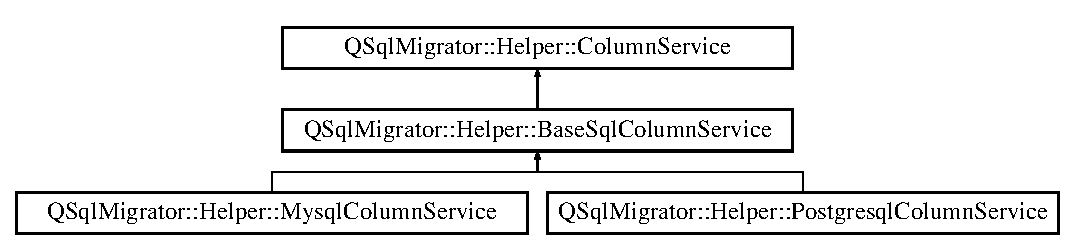
\includegraphics[height=2.906574cm]{class_q_sql_migrator_1_1_helper_1_1_column_service}
\end{center}
\end{figure}
\subsection*{Public Member Functions}
\begin{DoxyCompactItemize}
\item 
\mbox{\Hypertarget{class_q_sql_migrator_1_1_helper_1_1_column_service_aa3adb01c524afc209a029a803f9ff177}\label{class_q_sql_migrator_1_1_helper_1_1_column_service_aa3adb01c524afc209a029a803f9ff177}} 
virtual Q\+String {\bfseries generate\+Column\+Definition\+Sql} (const \hyperlink{class_q_sql_migrator_1_1_structure_1_1_column}{Structure\+::\+Column} \&column) const =0
\item 
\mbox{\Hypertarget{class_q_sql_migrator_1_1_helper_1_1_column_service_a785bde5004e7a4a4daf909c169b7e27c}\label{class_q_sql_migrator_1_1_helper_1_1_column_service_a785bde5004e7a4a4daf909c169b7e27c}} 
virtual Q\+String {\bfseries generate\+Columns\+Definition\+Sql} (const Q\+List$<$ \hyperlink{class_q_sql_migrator_1_1_structure_1_1_column}{Structure\+::\+Column} $>$ \&column\+List) const =0
\item 
\mbox{\Hypertarget{class_q_sql_migrator_1_1_helper_1_1_column_service_ae6384025ff1f65772b1f249286fd35e8}\label{class_q_sql_migrator_1_1_helper_1_1_column_service_ae6384025ff1f65772b1f249286fd35e8}} 
virtual Q\+String {\bfseries generate\+Index\+Column\+Definition\+Sql} (const \hyperlink{class_q_sql_migrator_1_1_structure_1_1_index_1_1_column}{Structure\+::\+Index\+::\+Column} \&column) const =0
\item 
\mbox{\Hypertarget{class_q_sql_migrator_1_1_helper_1_1_column_service_add05b75bd7c1bbcd8d7dc54445623ac9}\label{class_q_sql_migrator_1_1_helper_1_1_column_service_add05b75bd7c1bbcd8d7dc54445623ac9}} 
virtual Q\+String {\bfseries generate\+Index\+Columns\+Definition\+Sql} (const Structure\+::\+Index\+::\+Column\+List \&columns) const =0
\end{DoxyCompactItemize}


\subsection{Detailed Description}
interface for a service that can convert column and index definitions to proper S\+QL statements 

The documentation for this class was generated from the following file\+:\begin{DoxyCompactItemize}
\item 
/home/george/\+Develop/\+Praaline\+Py/praaline-\/core/\+Q\+Sql\+Migrator/\+Helper/Column\+Service.\+h\end{DoxyCompactItemize}

\hypertarget{class_q_sql_migrator_1_1_command_execution_1_1_command_execution_context}{}\section{Q\+Sql\+Migrator\+:\+:Command\+Execution\+:\+:Command\+Execution\+Context Class Reference}
\label{class_q_sql_migrator_1_1_command_execution_1_1_command_execution_context}\index{Q\+Sql\+Migrator\+::\+Command\+Execution\+::\+Command\+Execution\+Context@{Q\+Sql\+Migrator\+::\+Command\+Execution\+::\+Command\+Execution\+Context}}
\subsection*{Public Member Functions}
\begin{DoxyCompactItemize}
\item 
\mbox{\Hypertarget{class_q_sql_migrator_1_1_command_execution_1_1_command_execution_context_a9833f37d1f355e9acf705c17c7a24a8a}\label{class_q_sql_migrator_1_1_command_execution_1_1_command_execution_context_a9833f37d1f355e9acf705c17c7a24a8a}} 
{\bfseries Command\+Execution\+Context} (const Q\+Sql\+Database database, const \hyperlink{struct_q_sql_migrator_1_1_migration_execution_1_1_migration_execution_config}{Migration\+Execution\+::\+Migration\+Execution\+Config} \&migration\+Config, const \hyperlink{class_q_sql_migrator_1_1_helper_1_1_helper_repository}{Helper\+::\+Helper\+Repository} \&helper\+Repository)
\item 
\mbox{\Hypertarget{class_q_sql_migrator_1_1_command_execution_1_1_command_execution_context_ada9b80a7a767c3bb756a7a7c18c4e88d}\label{class_q_sql_migrator_1_1_command_execution_1_1_command_execution_context_ada9b80a7a767c3bb756a7a7c18c4e88d}} 
Q\+Sql\+Database {\bfseries database} () const
\item 
bool \hyperlink{class_q_sql_migrator_1_1_command_execution_1_1_command_execution_context_a48821a3965e12db6d06cfefcb103df2e}{is\+Undo\+Used} () const
\item 
\mbox{\Hypertarget{class_q_sql_migrator_1_1_command_execution_1_1_command_execution_context_af52d5b954891e5b255de55986d8ced0a}\label{class_q_sql_migrator_1_1_command_execution_1_1_command_execution_context_af52d5b954891e5b255de55986d8ced0a}} 
Commands\+::\+Command\+Ptr {\bfseries current\+Undo\+Command} () const
\item 
\mbox{\Hypertarget{class_q_sql_migrator_1_1_command_execution_1_1_command_execution_context_a3d53a72137b6684d3210e4c4983b2b45}\label{class_q_sql_migrator_1_1_command_execution_1_1_command_execution_context_a3d53a72137b6684d3210e4c4983b2b45}} 
const \hyperlink{struct_q_sql_migrator_1_1_migration_execution_1_1_migration_execution_config}{Migration\+Execution\+::\+Migration\+Execution\+Config} \& {\bfseries migration\+Config} () const
\item 
\mbox{\Hypertarget{class_q_sql_migrator_1_1_command_execution_1_1_command_execution_context_adaa22f2bad3aa78cf897c9ca6b30539d}\label{class_q_sql_migrator_1_1_command_execution_1_1_command_execution_context_adaa22f2bad3aa78cf897c9ca6b30539d}} 
const \hyperlink{class_q_sql_migrator_1_1_helper_1_1_helper_repository}{Helper\+::\+Helper\+Repository} \& {\bfseries helper\+Repository} () const
\item 
\mbox{\Hypertarget{class_q_sql_migrator_1_1_command_execution_1_1_command_execution_context_aa4999861869b7796ff6fc4bd7830f505}\label{class_q_sql_migrator_1_1_command_execution_1_1_command_execution_context_aa4999861869b7796ff6fc4bd7830f505}} 
void {\bfseries set\+Is\+Undo\+Used} (bool \hyperlink{class_q_sql_migrator_1_1_command_execution_1_1_command_execution_context_a48821a3965e12db6d06cfefcb103df2e}{is\+Undo\+Used})
\item 
\mbox{\Hypertarget{class_q_sql_migrator_1_1_command_execution_1_1_command_execution_context_a061187172723022ba4cd19c45a7a3838}\label{class_q_sql_migrator_1_1_command_execution_1_1_command_execution_context_a061187172723022ba4cd19c45a7a3838}} 
void {\bfseries set\+Undo\+Command} (Commands\+::\+Command\+Ptr command)
\item 
\mbox{\Hypertarget{class_q_sql_migrator_1_1_command_execution_1_1_command_execution_context_a2045c234885e2e9e3a475eb9e2a0a6f5}\label{class_q_sql_migrator_1_1_command_execution_1_1_command_execution_context_a2045c234885e2e9e3a475eb9e2a0a6f5}} 
void {\bfseries reset\+Undo\+Command} ()
\end{DoxyCompactItemize}


\subsection{Member Function Documentation}
\mbox{\Hypertarget{class_q_sql_migrator_1_1_command_execution_1_1_command_execution_context_a48821a3965e12db6d06cfefcb103df2e}\label{class_q_sql_migrator_1_1_command_execution_1_1_command_execution_context_a48821a3965e12db6d06cfefcb103df2e}} 
\index{Q\+Sql\+Migrator\+::\+Command\+Execution\+::\+Command\+Execution\+Context@{Q\+Sql\+Migrator\+::\+Command\+Execution\+::\+Command\+Execution\+Context}!is\+Undo\+Used@{is\+Undo\+Used}}
\index{is\+Undo\+Used@{is\+Undo\+Used}!Q\+Sql\+Migrator\+::\+Command\+Execution\+::\+Command\+Execution\+Context@{Q\+Sql\+Migrator\+::\+Command\+Execution\+::\+Command\+Execution\+Context}}
\subsubsection{\texorpdfstring{is\+Undo\+Used()}{isUndoUsed()}}
{\footnotesize\ttfamily bool Q\+Sql\+Migrator\+::\+Command\+Execution\+::\+Command\+Execution\+Context\+::is\+Undo\+Used (\begin{DoxyParamCaption}{ }\end{DoxyParamCaption}) const}

\begin{DoxyReturn}{Returns}
true, when undo command will be used 
\end{DoxyReturn}


The documentation for this class was generated from the following files\+:\begin{DoxyCompactItemize}
\item 
/home/george/\+Develop/\+Praaline\+Py/praaline-\/core/\+Q\+Sql\+Migrator/\+Command\+Execution/Command\+Execution\+Context.\+h\item 
/home/george/\+Develop/\+Praaline\+Py/praaline-\/core/\+Q\+Sql\+Migrator/\+Command\+Execution/Command\+Execution\+Context.\+cpp\end{DoxyCompactItemize}

\hypertarget{class_q_sql_migrator_1_1_command_execution_1_1_command_execution_service}{}\section{Q\+Sql\+Migrator\+:\+:Command\+Execution\+:\+:Command\+Execution\+Service Class Reference}
\label{class_q_sql_migrator_1_1_command_execution_1_1_command_execution_service}\index{Q\+Sql\+Migrator\+::\+Command\+Execution\+::\+Command\+Execution\+Service@{Q\+Sql\+Migrator\+::\+Command\+Execution\+::\+Command\+Execution\+Service}}
\subsection*{Public Member Functions}
\begin{DoxyCompactItemize}
\item 
\mbox{\Hypertarget{class_q_sql_migrator_1_1_command_execution_1_1_command_execution_service_ad4414f148b8948ac183abb64e27830b5}\label{class_q_sql_migrator_1_1_command_execution_1_1_command_execution_service_ad4414f148b8948ac183abb64e27830b5}} 
bool {\bfseries execute} (const Commands\+::\+Command\+Ptr command, Command\+Service\+Repository\+Ptr service\+Repository, \hyperlink{class_q_sql_migrator_1_1_command_execution_1_1_command_execution_context}{Command\+Execution\+Context} \&service\+Context) const
\item 
\mbox{\Hypertarget{class_q_sql_migrator_1_1_command_execution_1_1_command_execution_service_a22f05daa1823456f59d9749cef034381}\label{class_q_sql_migrator_1_1_command_execution_1_1_command_execution_service_a22f05daa1823456f59d9749cef034381}} 
bool {\bfseries batch} (const Commands\+::\+Command\+Ptr\+List \&command\+List, Commands\+::\+Command\+Ptr\+List \&undo\+Commands, Command\+Service\+Repository\+Ptr service\+Repository, \hyperlink{class_q_sql_migrator_1_1_command_execution_1_1_command_execution_context}{Command\+Execution\+Context} \&context) const
\end{DoxyCompactItemize}


The documentation for this class was generated from the following files\+:\begin{DoxyCompactItemize}
\item 
/home/george/\+Develop/\+Praaline\+Py/praaline-\/core/\+Q\+Sql\+Migrator/\+Command\+Execution/Command\+Execution\+Service.\+h\item 
/home/george/\+Develop/\+Praaline\+Py/praaline-\/core/\+Q\+Sql\+Migrator/\+Command\+Execution/Command\+Execution\+Service.\+cpp\end{DoxyCompactItemize}

\hypertarget{class_q_sql_migrator_1_1_command_execution_1_1_command_execution_service_repository}{}\section{Q\+Sql\+Migrator\+:\+:Command\+Execution\+:\+:Command\+Execution\+Service\+Repository Class Reference}
\label{class_q_sql_migrator_1_1_command_execution_1_1_command_execution_service_repository}\index{Q\+Sql\+Migrator\+::\+Command\+Execution\+::\+Command\+Execution\+Service\+Repository@{Q\+Sql\+Migrator\+::\+Command\+Execution\+::\+Command\+Execution\+Service\+Repository}}
\subsection*{Public Member Functions}
\begin{DoxyCompactItemize}
\item 
\mbox{\Hypertarget{class_q_sql_migrator_1_1_command_execution_1_1_command_execution_service_repository_a8ee67b70ed0a9ece4cbeb927dece8660}\label{class_q_sql_migrator_1_1_command_execution_1_1_command_execution_service_repository_a8ee67b70ed0a9ece4cbeb927dece8660}} 
Command\+Execution\+::\+Base\+Command\+Service\+Ptr {\bfseries get\+Service} (const Q\+String \&command\+Name) const
\item 
\mbox{\Hypertarget{class_q_sql_migrator_1_1_command_execution_1_1_command_execution_service_repository_abd9a974dec7b53fecaddbfd9af2fd0ff}\label{class_q_sql_migrator_1_1_command_execution_1_1_command_execution_service_repository_abd9a974dec7b53fecaddbfd9af2fd0ff}} 
void {\bfseries add} (Base\+Command\+Service\+Ptr service)
\end{DoxyCompactItemize}


The documentation for this class was generated from the following files\+:\begin{DoxyCompactItemize}
\item 
/home/george/\+Develop/\+Praaline\+Py/praaline-\/core/\+Q\+Sql\+Migrator/\+Command\+Execution/Command\+Execution\+Service\+Repository.\+h\item 
/home/george/\+Develop/\+Praaline\+Py/praaline-\/core/\+Q\+Sql\+Migrator/\+Command\+Execution/Command\+Execution\+Service\+Repository.\+cpp\end{DoxyCompactItemize}

\hypertarget{struct_query_filter_sequence_1_1_condition}{}\section{Query\+Filter\+Sequence\+:\+:Condition Struct Reference}
\label{struct_query_filter_sequence_1_1_condition}\index{Query\+Filter\+Sequence\+::\+Condition@{Query\+Filter\+Sequence\+::\+Condition}}
\subsection*{Public Member Functions}
\begin{DoxyCompactItemize}
\item 
\mbox{\Hypertarget{struct_query_filter_sequence_1_1_condition_a0a920994b04c9da78f681ff5af694d3e}\label{struct_query_filter_sequence_1_1_condition_a0a920994b04c9da78f681ff5af694d3e}} 
{\bfseries Condition} (Operand operand, Q\+Variant value)
\end{DoxyCompactItemize}
\subsection*{Public Attributes}
\begin{DoxyCompactItemize}
\item 
\mbox{\Hypertarget{struct_query_filter_sequence_1_1_condition_a24d5a6001f659ea93a2ae450d1dc1508}\label{struct_query_filter_sequence_1_1_condition_a24d5a6001f659ea93a2ae450d1dc1508}} 
Operand {\bfseries operand}
\item 
\mbox{\Hypertarget{struct_query_filter_sequence_1_1_condition_ae0243c75f0555a7f29e355f2a880209b}\label{struct_query_filter_sequence_1_1_condition_ae0243c75f0555a7f29e355f2a880209b}} 
Q\+Variant {\bfseries value}
\end{DoxyCompactItemize}


The documentation for this struct was generated from the following file\+:\begin{DoxyCompactItemize}
\item 
/home/george/\+Develop/\+Praaline\+Py/praaline-\/core/query/Query\+Filter\+Sequence.\+h\end{DoxyCompactItemize}

\hypertarget{class_co_n_l_l_x_document}{}\section{Co\+N\+L\+L\+X\+Document Class Reference}
\label{class_co_n_l_l_x_document}\index{Co\+N\+L\+L\+X\+Document@{Co\+N\+L\+L\+X\+Document}}


The documentation for this class was generated from the following files\+:\begin{DoxyCompactItemize}
\item 
/home/george/\+Develop/\+Praaline\+Py/praaline-\/core/interfaces/conll/Co\+N\+L\+L\+X\+Document.\+h\item 
/home/george/\+Develop/\+Praaline\+Py/praaline-\/core/interfaces/conll/Co\+N\+L\+L\+X\+Document.\+cpp\end{DoxyCompactItemize}

\hypertarget{class_corpus}{}\section{Corpus Class Reference}
\label{class_corpus}\index{Corpus@{Corpus}}
Inheritance diagram for Corpus\+:\begin{figure}[H]
\begin{center}
\leavevmode
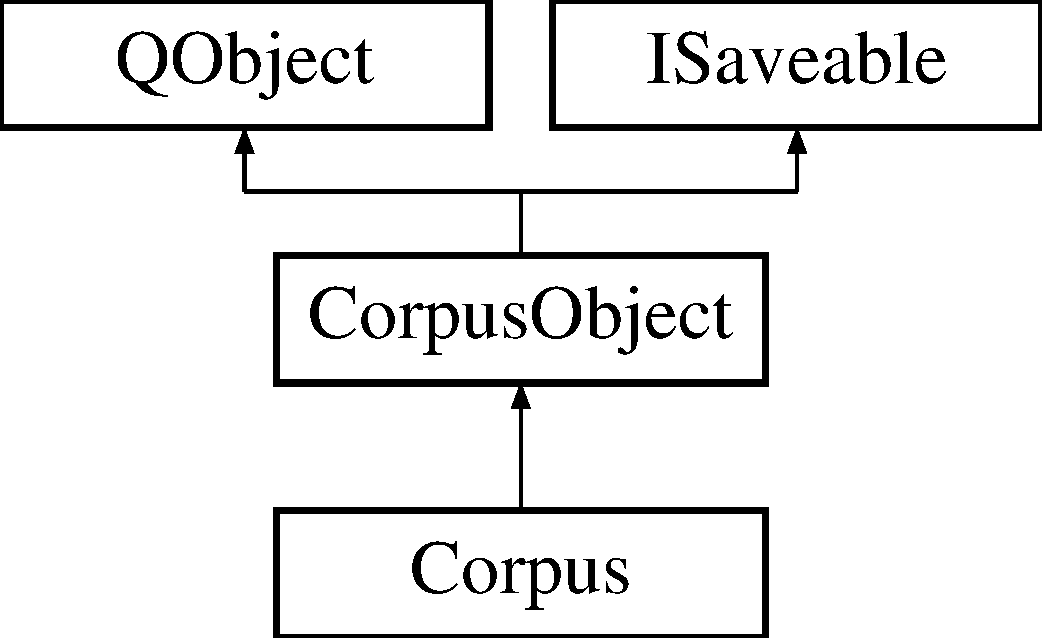
\includegraphics[height=3.000000cm]{class_corpus}
\end{center}
\end{figure}
\subsection*{Signals}
\begin{DoxyCompactItemize}
\item 
\mbox{\Hypertarget{class_corpus_af27c09a3d9a2cdd3307f133331e8af81}\label{class_corpus_af27c09a3d9a2cdd3307f133331e8af81}} 
void {\bfseries communication\+Added} (Q\+Pointer$<$ P\+R\+A\+A\+L\+I\+N\+E\+\_\+\+C\+O\+R\+E\+\_\+\+N\+A\+M\+E\+S\+P\+A\+C\+E\+::\+Corpus\+Communication $>$ communication)
\item 
\mbox{\Hypertarget{class_corpus_a0ae2650c2acc7495ed72d4501ef43df7}\label{class_corpus_a0ae2650c2acc7495ed72d4501ef43df7}} 
void {\bfseries communication\+Deleted} (Q\+String ID)
\item 
\mbox{\Hypertarget{class_corpus_a6a2a743b27ef679643e316df3d5c06a6}\label{class_corpus_a6a2a743b27ef679643e316df3d5c06a6}} 
void {\bfseries speaker\+Added} (Q\+Pointer$<$ P\+R\+A\+A\+L\+I\+N\+E\+\_\+\+C\+O\+R\+E\+\_\+\+N\+A\+M\+E\+S\+P\+A\+C\+E\+::\+Corpus\+Speaker $>$ speaker)
\item 
\mbox{\Hypertarget{class_corpus_a4701e900ef2d20093c31e81ab23f32db}\label{class_corpus_a4701e900ef2d20093c31e81ab23f32db}} 
void {\bfseries speaker\+Deleted} (Q\+String ID)
\end{DoxyCompactItemize}
\subsection*{Public Member Functions}
\begin{DoxyCompactItemize}
\item 
\mbox{\Hypertarget{class_corpus_a425510e7043059892721f9e277f67e21}\label{class_corpus_a425510e7043059892721f9e277f67e21}} 
{\bfseries Corpus} (\hyperlink{class_corpus_repository}{Corpus\+Repository} $\ast$repository=nullptr, Q\+Object $\ast$parent=nullptr)
\item 
\mbox{\Hypertarget{class_corpus_acd2fb05316e98fe719db3e393155168c}\label{class_corpus_acd2fb05316e98fe719db3e393155168c}} 
{\bfseries Corpus} (const Q\+String \&ID, \hyperlink{class_corpus_repository}{Corpus\+Repository} $\ast$repository=nullptr, Q\+Object $\ast$parent=nullptr)
\item 
\mbox{\Hypertarget{class_corpus_a4ca235852ae565699aa6f94574c6ed08}\label{class_corpus_a4ca235852ae565699aa6f94574c6ed08}} 
Corpus\+Object\+::\+Type {\bfseries type} () const override
\item 
\mbox{\Hypertarget{class_corpus_ac1a90bbf167ae15bb9e60f763b7613c4}\label{class_corpus_ac1a90bbf167ae15bb9e60f763b7613c4}} 
bool {\bfseries save} () override
\item 
\mbox{\Hypertarget{class_corpus_aace59ec0a90b8e0dc38baf8503403ea8}\label{class_corpus_aace59ec0a90b8e0dc38baf8503403ea8}} 
Q\+String {\bfseries name} () const
\item 
\mbox{\Hypertarget{class_corpus_a7ec330802b109beac27c3563d36d20b6}\label{class_corpus_a7ec330802b109beac27c3563d36d20b6}} 
void {\bfseries set\+Name} (const Q\+String \&name)
\item 
\mbox{\Hypertarget{class_corpus_a56289ebc4858576a1f61718b1682c020}\label{class_corpus_a56289ebc4858576a1f61718b1682c020}} 
Q\+String {\bfseries description} () const
\item 
\mbox{\Hypertarget{class_corpus_a450f7f3e3ce0437d250d3f68bbd49878}\label{class_corpus_a450f7f3e3ce0437d250d3f68bbd49878}} 
void {\bfseries set\+Description} (const Q\+String \&description)
\item 
\mbox{\Hypertarget{class_corpus_a4bac5617957f76e1c621292ad4de507e}\label{class_corpus_a4bac5617957f76e1c621292ad4de507e}} 
Q\+String {\bfseries corpus\+ID} () const override
\item 
\mbox{\Hypertarget{class_corpus_a6683210f37ceae87bd37515e8cdcf996}\label{class_corpus_a6683210f37ceae87bd37515e8cdcf996}} 
void {\bfseries set\+Corpus\+ID} (const Q\+String \&corpus\+ID) override
\item 
\mbox{\Hypertarget{class_corpus_a84087660b16d31d547ea3e7dc1b45088}\label{class_corpus_a84087660b16d31d547ea3e7dc1b45088}} 
void {\bfseries clear} ()
\item 
\mbox{\Hypertarget{class_corpus_a5f63f21382d9a9c0de14d31df01c8bab}\label{class_corpus_a5f63f21382d9a9c0de14d31df01c8bab}} 
Q\+Pointer$<$ \hyperlink{class_corpus_communication}{Corpus\+Communication} $>$ {\bfseries communication} (const Q\+String \&communication\+ID) const
\item 
\mbox{\Hypertarget{class_corpus_aa5a929a8e3d10b5851a7ba6ad064c12a}\label{class_corpus_aa5a929a8e3d10b5851a7ba6ad064c12a}} 
int {\bfseries communications\+Count} () const
\item 
\mbox{\Hypertarget{class_corpus_aae5348f25de705df3cb6e7ddbb1cf186}\label{class_corpus_aae5348f25de705df3cb6e7ddbb1cf186}} 
bool {\bfseries has\+Communications} () const
\item 
\mbox{\Hypertarget{class_corpus_a52ba6fa1f3c0ecad726d8426d209800a}\label{class_corpus_a52ba6fa1f3c0ecad726d8426d209800a}} 
bool {\bfseries has\+Communication} (const Q\+String \&communication\+ID) const
\item 
\mbox{\Hypertarget{class_corpus_aef989baa3a11224defcd318e9aa32d1f}\label{class_corpus_aef989baa3a11224defcd318e9aa32d1f}} 
Q\+String\+List {\bfseries communication\+I\+Ds} () const
\item 
\mbox{\Hypertarget{class_corpus_a69e0227e1b170f27ae30fdddf858427f}\label{class_corpus_a69e0227e1b170f27ae30fdddf858427f}} 
const Q\+Map$<$ Q\+String, Q\+Pointer$<$ \hyperlink{class_corpus_communication}{Corpus\+Communication} $>$ $>$ \& {\bfseries communications} () const
\item 
\mbox{\Hypertarget{class_corpus_a26f495a4c45cb80de5ca8260caf1253e}\label{class_corpus_a26f495a4c45cb80de5ca8260caf1253e}} 
void {\bfseries add\+Communication} (\hyperlink{class_corpus_communication}{Corpus\+Communication} $\ast$communication)
\item 
\mbox{\Hypertarget{class_corpus_a1a30199fd871a0a5508dc8fd836cbc15}\label{class_corpus_a1a30199fd871a0a5508dc8fd836cbc15}} 
void {\bfseries remove\+Communication} (const Q\+String \&communication\+ID)
\item 
\mbox{\Hypertarget{class_corpus_ad8bf012af653dc02f0a2704f52d3c098}\label{class_corpus_ad8bf012af653dc02f0a2704f52d3c098}} 
Q\+Pointer$<$ \hyperlink{class_corpus_speaker}{Corpus\+Speaker} $>$ {\bfseries speaker} (const Q\+String \&speaker\+ID) const
\item 
\mbox{\Hypertarget{class_corpus_aad27cde20185492a31efaa395aa7d207}\label{class_corpus_aad27cde20185492a31efaa395aa7d207}} 
int {\bfseries speakers\+Count} () const
\item 
\mbox{\Hypertarget{class_corpus_a6245c2836161c1f53122ec7ff1664676}\label{class_corpus_a6245c2836161c1f53122ec7ff1664676}} 
bool {\bfseries has\+Speakers} () const
\item 
\mbox{\Hypertarget{class_corpus_ad0b26394149fd83fab56d33c5e8fd066}\label{class_corpus_ad0b26394149fd83fab56d33c5e8fd066}} 
bool {\bfseries has\+Speaker} (const Q\+String \&speaker\+ID) const
\item 
\mbox{\Hypertarget{class_corpus_a4056b10d0459bf42642662edd6ef2cac}\label{class_corpus_a4056b10d0459bf42642662edd6ef2cac}} 
Q\+String\+List {\bfseries speaker\+I\+Ds} () const
\item 
\mbox{\Hypertarget{class_corpus_aeaefdb0df0474809ebb6175474a25300}\label{class_corpus_aeaefdb0df0474809ebb6175474a25300}} 
const Q\+Map$<$ Q\+String, Q\+Pointer$<$ \hyperlink{class_corpus_speaker}{Corpus\+Speaker} $>$ $>$ \& {\bfseries speakers} () const
\item 
\mbox{\Hypertarget{class_corpus_a1617afc5ac5f265cd16a1b964056da23}\label{class_corpus_a1617afc5ac5f265cd16a1b964056da23}} 
void {\bfseries add\+Speaker} (\hyperlink{class_corpus_speaker}{Corpus\+Speaker} $\ast$speaker)
\item 
\mbox{\Hypertarget{class_corpus_af6fbce091bf2a5d9199a82d3318ccd27}\label{class_corpus_af6fbce091bf2a5d9199a82d3318ccd27}} 
void {\bfseries remove\+Speaker} (const Q\+String \&speaker\+ID)
\item 
\mbox{\Hypertarget{class_corpus_aae0f04111009345b6fccd7acdd3e256d}\label{class_corpus_aae0f04111009345b6fccd7acdd3e256d}} 
Q\+Pointer$<$ \hyperlink{class_corpus_participation}{Corpus\+Participation} $>$ {\bfseries participation} (const Q\+String \&communication\+ID, const Q\+String \&speaker\+ID)
\item 
\mbox{\Hypertarget{class_corpus_af0268bc3c38da2fc5aef539f9f51ce74}\label{class_corpus_af0268bc3c38da2fc5aef539f9f51ce74}} 
bool {\bfseries has\+Participation} (const Q\+String \&communication\+ID, const Q\+String \&speaker\+ID)
\item 
\mbox{\Hypertarget{class_corpus_a69e657d9da48943dcbce81925a705569}\label{class_corpus_a69e657d9da48943dcbce81925a705569}} 
Q\+List$<$ Q\+Pointer$<$ \hyperlink{class_corpus_participation}{Corpus\+Participation} $>$ $>$ {\bfseries participations} ()
\item 
\mbox{\Hypertarget{class_corpus_a7b96f1346c6cc6394b6f2c88ef226767}\label{class_corpus_a7b96f1346c6cc6394b6f2c88ef226767}} 
Q\+List$<$ Q\+Pointer$<$ \hyperlink{class_corpus_participation}{Corpus\+Participation} $>$ $>$ {\bfseries participations\+For\+Communication} (const Q\+String \&communication\+ID)
\item 
\mbox{\Hypertarget{class_corpus_adb290afffa993f7232932e9e7a6fe10e}\label{class_corpus_adb290afffa993f7232932e9e7a6fe10e}} 
Q\+List$<$ Q\+Pointer$<$ \hyperlink{class_corpus_participation}{Corpus\+Participation} $>$ $>$ {\bfseries participations\+For\+Speaker} (const Q\+String \&speaker\+ID)
\item 
\mbox{\Hypertarget{class_corpus_a1fdd32d24c55b4f9a477efdb68df52ad}\label{class_corpus_a1fdd32d24c55b4f9a477efdb68df52ad}} 
Q\+Pointer$<$ \hyperlink{class_corpus_participation}{Corpus\+Participation} $>$ {\bfseries add\+Participation} (const Q\+String \&communication\+ID, const Q\+String \&speaker\+ID, const Q\+String \&role=Q\+String())
\item 
\mbox{\Hypertarget{class_corpus_ac1c54f5078d3eb9de6063c38e6fbb6e0}\label{class_corpus_ac1c54f5078d3eb9de6063c38e6fbb6e0}} 
void {\bfseries remove\+Participation} (const Q\+String \&communication\+ID, const Q\+String \&speaker\+ID)
\item 
\mbox{\Hypertarget{class_corpus_aa1169b1871f4b115d012c7f2d6e703ce}\label{class_corpus_aa1169b1871f4b115d012c7f2d6e703ce}} 
Q\+String\+List {\bfseries recording\+I\+Ds} () const
\item 
\mbox{\Hypertarget{class_corpus_a11fb88253c81a672bc12a1fe11de1dc4}\label{class_corpus_a11fb88253c81a672bc12a1fe11de1dc4}} 
Q\+String\+List {\bfseries annotation\+I\+Ds} () const
\item 
\mbox{\Hypertarget{class_corpus_aea431975c8d338bb216ff5d47b114f10}\label{class_corpus_aea431975c8d338bb216ff5d47b114f10}} 
Q\+List$<$ Q\+Pointer$<$ \hyperlink{class_corpus_communication}{Corpus\+Communication} $>$ $>$ {\bfseries communications\+List} () const
\item 
\mbox{\Hypertarget{class_corpus_af334c719b11e7de4ec00acc8d68ff895}\label{class_corpus_af334c719b11e7de4ec00acc8d68ff895}} 
Q\+List$<$ Q\+Pointer$<$ \hyperlink{class_corpus_speaker}{Corpus\+Speaker} $>$ $>$ {\bfseries speakers\+List} () const
\item 
\mbox{\Hypertarget{class_corpus_ac46407c550be94dee0483190d1c5dd08}\label{class_corpus_ac46407c550be94dee0483190d1c5dd08}} 
Q\+List$<$ Q\+Pointer$<$ \hyperlink{class_corpus_recording}{Corpus\+Recording} $>$ $>$ {\bfseries recordings\+List} () const
\item 
\mbox{\Hypertarget{class_corpus_ad4f2b0f294d0bc936cfe0fdeb01df384}\label{class_corpus_ad4f2b0f294d0bc936cfe0fdeb01df384}} 
Q\+List$<$ Q\+Pointer$<$ \hyperlink{class_corpus_annotation}{Corpus\+Annotation} $>$ $>$ {\bfseries annotations\+List} () const
\item 
\mbox{\Hypertarget{class_corpus_abd5174294912f577ba912c7d7fe3990f}\label{class_corpus_abd5174294912f577ba912c7d7fe3990f}} 
Q\+Map$<$ Q\+String, Q\+Pair$<$ Q\+Pointer$<$ \hyperlink{class_corpus_recording}{Corpus\+Recording} $>$, Q\+Pointer$<$ \hyperlink{class_corpus_annotation}{Corpus\+Annotation} $>$ $>$ $>$ {\bfseries get\+Recordings\+\_\+x\+\_\+\+Annotations} () const
\item 
\mbox{\Hypertarget{class_corpus_a44b6483e0cea2f124272ce79905ba05f}\label{class_corpus_a44b6483e0cea2f124272ce79905ba05f}} 
Q\+Map$<$ Q\+String, Q\+Pair$<$ Q\+Pointer$<$ \hyperlink{class_corpus_annotation}{Corpus\+Annotation} $>$, Q\+Pointer$<$ \hyperlink{class_corpus_recording}{Corpus\+Recording} $>$ $>$ $>$ {\bfseries get\+Annotations\+\_\+x\+\_\+\+Recordings} () const
\item 
\mbox{\Hypertarget{class_corpus_aeb1454b56f0e11cf8ae5f91f8d6f4c1e}\label{class_corpus_aeb1454b56f0e11cf8ae5f91f8d6f4c1e}} 
Q\+List$<$ Q\+Pair$<$ Q\+String, Q\+String $>$ $>$ {\bfseries get\+Communications\+Annotations\+I\+Ds} () const
\item 
\mbox{\Hypertarget{class_corpus_ae84db3aaf9ad1b0cae5fac3196b77088}\label{class_corpus_ae84db3aaf9ad1b0cae5fac3196b77088}} 
Q\+List$<$ Q\+Pair$<$ Q\+String, Q\+String $>$ $>$ {\bfseries get\+Communications\+Recordings\+I\+Ds} () const
\end{DoxyCompactItemize}
\subsection*{Public Attributes}
\begin{DoxyCompactItemize}
\item 
\mbox{\Hypertarget{class_corpus_a55599dacff53f4ea699a1758f3a2aaeb}\label{class_corpus_a55599dacff53f4ea699a1758f3a2aaeb}} 
Q\+List$<$ Q\+String $>$ {\bfseries deleted\+Communication\+I\+Ds}
\item 
\mbox{\Hypertarget{class_corpus_adf9500d71cba6f1179681acbe17ca7af}\label{class_corpus_adf9500d71cba6f1179681acbe17ca7af}} 
Q\+List$<$ Q\+String $>$ {\bfseries deleted\+Speaker\+I\+Ds}
\item 
\mbox{\Hypertarget{class_corpus_a09ad0d669adf1007f31ea1786b6be918}\label{class_corpus_a09ad0d669adf1007f31ea1786b6be918}} 
Q\+List$<$ Q\+Pair$<$ Q\+String, Q\+String $>$ $>$ {\bfseries deleted\+Participation\+I\+Ds}
\end{DoxyCompactItemize}
\subsection*{Properties}
\begin{DoxyCompactItemize}
\item 
\mbox{\Hypertarget{class_corpus_a90e1ba1705b04ad6d58810afbf08d9cd}\label{class_corpus_a90e1ba1705b04ad6d58810afbf08d9cd}} 
Q\+String {\bfseries name}
\end{DoxyCompactItemize}
\subsection*{Additional Inherited Members}


The documentation for this class was generated from the following files\+:\begin{DoxyCompactItemize}
\item 
/home/george/\+Develop/\+Praaline\+Py/praaline-\/core/corpus/Corpus.\+h\item 
/home/george/\+Develop/\+Praaline\+Py/praaline-\/core/corpus/Corpus.\+cpp\end{DoxyCompactItemize}

\hypertarget{class_corpus_annotation}{}\section{Corpus\+Annotation Class Reference}
\label{class_corpus_annotation}\index{Corpus\+Annotation@{Corpus\+Annotation}}
Inheritance diagram for Corpus\+Annotation\+:\begin{figure}[H]
\begin{center}
\leavevmode
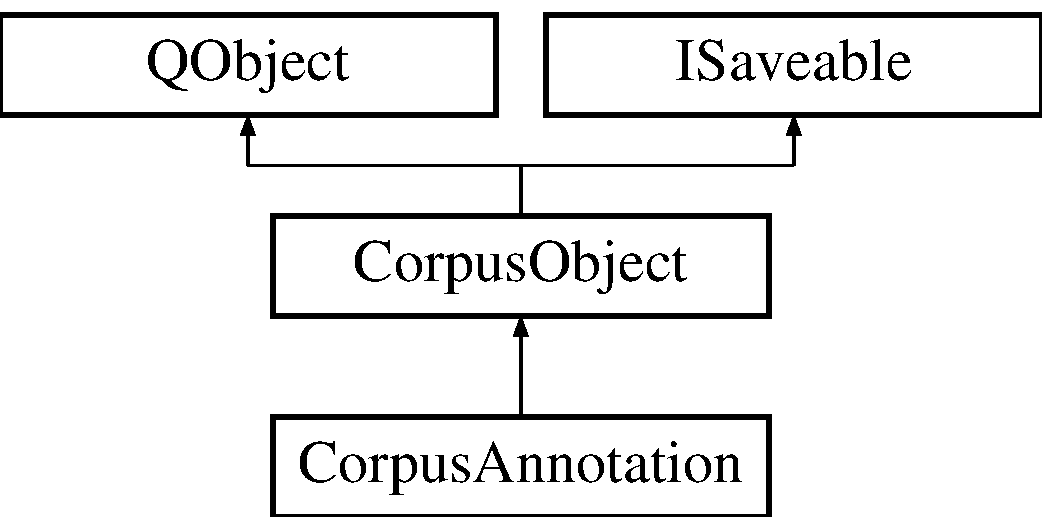
\includegraphics[height=3.000000cm]{class_corpus_annotation}
\end{center}
\end{figure}
\subsection*{Public Member Functions}
\begin{DoxyCompactItemize}
\item 
\mbox{\Hypertarget{class_corpus_annotation_aeaf4554895df52730ab8c6939b070421}\label{class_corpus_annotation_aeaf4554895df52730ab8c6939b070421}} 
{\bfseries Corpus\+Annotation} (\hyperlink{class_corpus_repository}{Corpus\+Repository} $\ast$repository=nullptr, Q\+Object $\ast$parent=nullptr)
\item 
\mbox{\Hypertarget{class_corpus_annotation_a23014f51ce94c4b90ac04ec2fce29938}\label{class_corpus_annotation_a23014f51ce94c4b90ac04ec2fce29938}} 
{\bfseries Corpus\+Annotation} (const Q\+String ID, \hyperlink{class_corpus_repository}{Corpus\+Repository} $\ast$repository=nullptr, Q\+Object $\ast$parent=nullptr)
\item 
\mbox{\Hypertarget{class_corpus_annotation_ad79f5199315b78ffa0da1ef06a687a93}\label{class_corpus_annotation_ad79f5199315b78ffa0da1ef06a687a93}} 
{\bfseries Corpus\+Annotation} (\hyperlink{class_corpus_annotation}{Corpus\+Annotation} $\ast$other, Q\+Object $\ast$parent=nullptr)
\item 
\mbox{\Hypertarget{class_corpus_annotation_adc7b62e91d01e00c9754aa8819841587}\label{class_corpus_annotation_adc7b62e91d01e00c9754aa8819841587}} 
Corpus\+Object\+::\+Type {\bfseries type} () const override
\item 
\mbox{\Hypertarget{class_corpus_annotation_ab6e98b3fc0d449b2e76b32ca25a27102}\label{class_corpus_annotation_ab6e98b3fc0d449b2e76b32ca25a27102}} 
bool {\bfseries save} () override
\item 
\mbox{\Hypertarget{class_corpus_annotation_af9a18d51ebb2e4db26bb66a831ea4c57}\label{class_corpus_annotation_af9a18d51ebb2e4db26bb66a831ea4c57}} 
Q\+String {\bfseries communication\+ID} () const
\item 
\mbox{\Hypertarget{class_corpus_annotation_a71af0d158027529d821a9fc41ddd888a}\label{class_corpus_annotation_a71af0d158027529d821a9fc41ddd888a}} 
Q\+Pointer$<$ \hyperlink{class_corpus}{Corpus} $>$ {\bfseries corpus} () const
\item 
\mbox{\Hypertarget{class_corpus_annotation_a3d96da8cc79294ad900ea8869ab040b4}\label{class_corpus_annotation_a3d96da8cc79294ad900ea8869ab040b4}} 
Q\+String {\bfseries name} () const
\item 
\mbox{\Hypertarget{class_corpus_annotation_a3cdc3692368c60cdde4bedcd22db525f}\label{class_corpus_annotation_a3cdc3692368c60cdde4bedcd22db525f}} 
void {\bfseries set\+Name} (const Q\+String \&name)
\item 
\mbox{\Hypertarget{class_corpus_annotation_ae64f1c514ad722bb7a8abe5052f22ace}\label{class_corpus_annotation_ae64f1c514ad722bb7a8abe5052f22ace}} 
Q\+String {\bfseries recording\+ID} () const
\item 
\mbox{\Hypertarget{class_corpus_annotation_a9955b82391b40b6c8c39c26b9036bd1b}\label{class_corpus_annotation_a9955b82391b40b6c8c39c26b9036bd1b}} 
void {\bfseries set\+Recording\+ID} (const Q\+String \&recording\+ID)
\item 
\mbox{\Hypertarget{class_corpus_annotation_af0a0a7c4128d6fa9b010e027571c195e}\label{class_corpus_annotation_af0a0a7c4128d6fa9b010e027571c195e}} 
Q\+String {\bfseries filename} () const
\item 
\mbox{\Hypertarget{class_corpus_annotation_aaa35e7b750a3735f8aa29fe2d2a79497}\label{class_corpus_annotation_aaa35e7b750a3735f8aa29fe2d2a79497}} 
void {\bfseries set\+Filename} (const Q\+String \&filename)
\item 
\mbox{\Hypertarget{class_corpus_annotation_ae058e5a667a46dd0faaba1268e589e0b}\label{class_corpus_annotation_ae058e5a667a46dd0faaba1268e589e0b}} 
Q\+String {\bfseries format} () const
\item 
\mbox{\Hypertarget{class_corpus_annotation_a09849335dcca310cd05cd92a19517ab0}\label{class_corpus_annotation_a09849335dcca310cd05cd92a19517ab0}} 
void {\bfseries set\+Format} (const Q\+String \&format)
\item 
\mbox{\Hypertarget{class_corpus_annotation_a3c8175817f0272d5d3fee3842b467190}\label{class_corpus_annotation_a3c8175817f0272d5d3fee3842b467190}} 
bool {\bfseries is\+Multi\+Language} () const
\item 
\mbox{\Hypertarget{class_corpus_annotation_a1e4de8bf7fee8f722898de91eca5f43c}\label{class_corpus_annotation_a1e4de8bf7fee8f722898de91eca5f43c}} 
Q\+String\+List {\bfseries languages} () const
\item 
\mbox{\Hypertarget{class_corpus_annotation_af0cf8b8b30fb75de053c300eea662df1}\label{class_corpus_annotation_af0cf8b8b30fb75de053c300eea662df1}} 
void {\bfseries add\+Language} (const Q\+String \&language\+ID)
\item 
\mbox{\Hypertarget{class_corpus_annotation_a0bfc429fa745f304b507b5a80568e12b}\label{class_corpus_annotation_a0bfc429fa745f304b507b5a80568e12b}} 
void {\bfseries remove\+Language} (const Q\+String \&language\+ID)
\end{DoxyCompactItemize}
\subsection*{Properties}
\begin{DoxyCompactItemize}
\item 
\mbox{\Hypertarget{class_corpus_annotation_a445c4bbf129abd28b244699ac6fa0c83}\label{class_corpus_annotation_a445c4bbf129abd28b244699ac6fa0c83}} 
Q\+String {\bfseries name}
\item 
\mbox{\Hypertarget{class_corpus_annotation_a2f719c17ffb4ddc3e5877b1120971eb6}\label{class_corpus_annotation_a2f719c17ffb4ddc3e5877b1120971eb6}} 
Q\+String {\bfseries filename}
\item 
\mbox{\Hypertarget{class_corpus_annotation_a3ac440c36ef040cb9e20173eb85f571b}\label{class_corpus_annotation_a3ac440c36ef040cb9e20173eb85f571b}} 
Q\+String {\bfseries format}
\item 
\mbox{\Hypertarget{class_corpus_annotation_ad9cabcfae5f6ea6aba1b66f9e5e92ab9}\label{class_corpus_annotation_ad9cabcfae5f6ea6aba1b66f9e5e92ab9}} 
Q\+String\+List {\bfseries languages}
\item 
\mbox{\Hypertarget{class_corpus_annotation_a10eea3344873ffd772f7cb43639a6678}\label{class_corpus_annotation_a10eea3344873ffd772f7cb43639a6678}} 
Q\+String {\bfseries communication\+ID}
\end{DoxyCompactItemize}
\subsection*{Additional Inherited Members}


The documentation for this class was generated from the following files\+:\begin{DoxyCompactItemize}
\item 
/home/george/\+Develop/\+Praaline\+Py/praaline-\/core/corpus/Corpus\+Annotation.\+h\item 
/home/george/\+Develop/\+Praaline\+Py/praaline-\/core/corpus/Corpus\+Annotation.\+cpp\end{DoxyCompactItemize}

\hypertarget{class_corpus_bookmark}{}\section{Corpus\+Bookmark Class Reference}
\label{class_corpus_bookmark}\index{Corpus\+Bookmark@{Corpus\+Bookmark}}
Inheritance diagram for Corpus\+Bookmark\+:\begin{figure}[H]
\begin{center}
\leavevmode
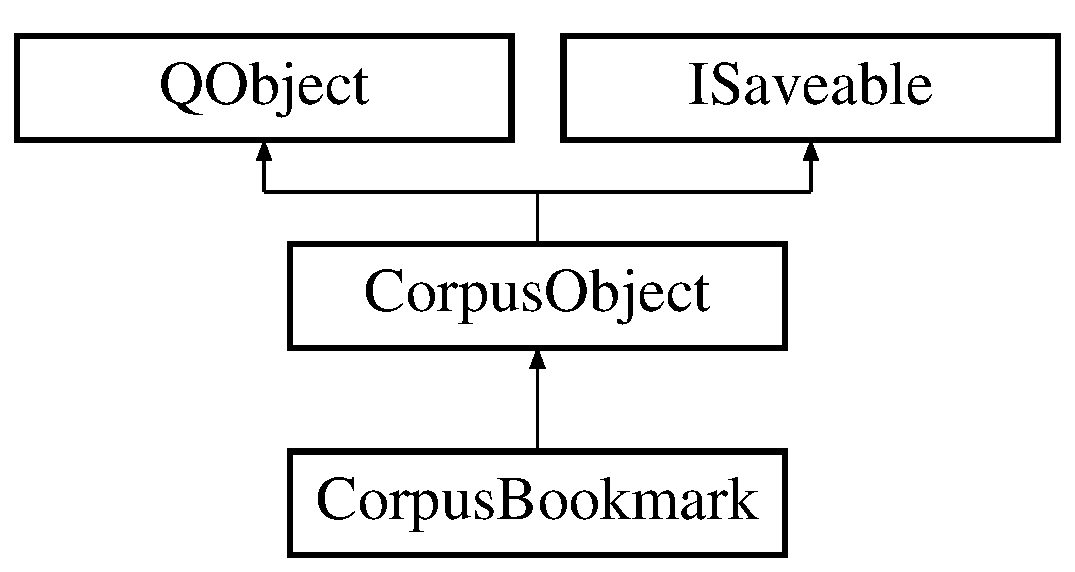
\includegraphics[height=3.000000cm]{class_corpus_bookmark}
\end{center}
\end{figure}
\subsection*{Public Member Functions}
\begin{DoxyCompactItemize}
\item 
\mbox{\Hypertarget{class_corpus_bookmark_a122599342d6bb2f6b6beae0d7a8ffece}\label{class_corpus_bookmark_a122599342d6bb2f6b6beae0d7a8ffece}} 
{\bfseries Corpus\+Bookmark} (Q\+Object $\ast$parent=nullptr)
\item 
\mbox{\Hypertarget{class_corpus_bookmark_afe16569951bdaeefd4aa0e1ca0da54c4}\label{class_corpus_bookmark_afe16569951bdaeefd4aa0e1ca0da54c4}} 
{\bfseries Corpus\+Bookmark} (const Q\+String \&corpus\+ID, const Q\+String \&communication\+ID, const Q\+String \&annotation\+ID, const \hyperlink{struct_real_time}{Real\+Time} \&time, const Q\+String \&name, const Q\+String \&notes=Q\+String(), Q\+Object $\ast$parent=nullptr)
\item 
\mbox{\Hypertarget{class_corpus_bookmark_af8bb4f7d5570f674626644a8e90d4384}\label{class_corpus_bookmark_af8bb4f7d5570f674626644a8e90d4384}} 
{\bfseries Corpus\+Bookmark} (const Q\+String \&corpus\+ID, const Q\+String \&communication\+ID, const Q\+String \&annotation\+ID, const \hyperlink{struct_real_time}{Real\+Time} \&time\+Start, const \hyperlink{struct_real_time}{Real\+Time} \&time\+End, const Q\+String \&name, const Q\+String \&notes=Q\+String(), Q\+Object $\ast$parent=nullptr)
\item 
\mbox{\Hypertarget{class_corpus_bookmark_a10899c6bdab48f5b6b1237cd61b4a726}\label{class_corpus_bookmark_a10899c6bdab48f5b6b1237cd61b4a726}} 
Q\+String {\bfseries ID} () const override
\item 
\mbox{\Hypertarget{class_corpus_bookmark_aed714ed4ef3f9a94eb408e4bc025dc37}\label{class_corpus_bookmark_aed714ed4ef3f9a94eb408e4bc025dc37}} 
void {\bfseries set\+ID} (const Q\+String \&ID) override
\item 
\mbox{\Hypertarget{class_corpus_bookmark_ababfd655298586a3d621a882ee416f99}\label{class_corpus_bookmark_ababfd655298586a3d621a882ee416f99}} 
Corpus\+Object\+::\+Type {\bfseries type} () const override
\item 
\mbox{\Hypertarget{class_corpus_bookmark_addc15dc499b80a28492005f9d6f5247e}\label{class_corpus_bookmark_addc15dc499b80a28492005f9d6f5247e}} 
bool {\bfseries save} () override
\item 
\mbox{\Hypertarget{class_corpus_bookmark_ac4d85da7d148a605745d688698d38e2d}\label{class_corpus_bookmark_ac4d85da7d148a605745d688698d38e2d}} 
Q\+String {\bfseries communication\+ID} () const
\item 
\mbox{\Hypertarget{class_corpus_bookmark_ac10293f4e2033746d695c6349805fcba}\label{class_corpus_bookmark_ac10293f4e2033746d695c6349805fcba}} 
Q\+String {\bfseries annotation\+ID} () const
\item 
\mbox{\Hypertarget{class_corpus_bookmark_a4567b01babc1074c21fd81fa4cf6b5bc}\label{class_corpus_bookmark_a4567b01babc1074c21fd81fa4cf6b5bc}} 
\hyperlink{struct_real_time}{Real\+Time} {\bfseries time} () const
\item 
\mbox{\Hypertarget{class_corpus_bookmark_a5954ecddfa90b9083ebca82ebf103d33}\label{class_corpus_bookmark_a5954ecddfa90b9083ebca82ebf103d33}} 
\hyperlink{struct_real_time}{Real\+Time} {\bfseries time\+Start} () const
\item 
\mbox{\Hypertarget{class_corpus_bookmark_ad4a33b45958e1a28eba0f659a94257f5}\label{class_corpus_bookmark_ad4a33b45958e1a28eba0f659a94257f5}} 
\hyperlink{struct_real_time}{Real\+Time} {\bfseries time\+End} () const
\item 
\mbox{\Hypertarget{class_corpus_bookmark_aecef3174b630fceda67dc4137f5ddcc4}\label{class_corpus_bookmark_aecef3174b630fceda67dc4137f5ddcc4}} 
\hyperlink{struct_real_time}{Real\+Time} {\bfseries duration} () const
\item 
\mbox{\Hypertarget{class_corpus_bookmark_a754ad425a41da641362b34452777c530}\label{class_corpus_bookmark_a754ad425a41da641362b34452777c530}} 
Q\+String {\bfseries name} () const
\item 
\mbox{\Hypertarget{class_corpus_bookmark_a08b19a694d6d4238342e09554eeb5735}\label{class_corpus_bookmark_a08b19a694d6d4238342e09554eeb5735}} 
Q\+String {\bfseries notes} () const
\item 
\mbox{\Hypertarget{class_corpus_bookmark_a3ad4e2e8fa63501f87b2f181bb125ddc}\label{class_corpus_bookmark_a3ad4e2e8fa63501f87b2f181bb125ddc}} 
void {\bfseries set} (const Q\+String \&corpus\+ID=Q\+String(), const Q\+String \&communication\+ID=Q\+String(), const Q\+String \&annotation\+ID=Q\+String(), const \hyperlink{struct_real_time}{Real\+Time} \&time=\hyperlink{struct_real_time}{Real\+Time}(-\/1, 0), const Q\+String \&name=Q\+String(), const Q\+String \&notes=Q\+String())
\item 
\mbox{\Hypertarget{class_corpus_bookmark_af45e5143ac43cd79bec171d240d8ab88}\label{class_corpus_bookmark_af45e5143ac43cd79bec171d240d8ab88}} 
void {\bfseries set} (const Q\+String \&corpus\+ID=Q\+String(), const Q\+String \&communication\+ID=Q\+String(), const Q\+String \&annotation\+ID=Q\+String(), const \hyperlink{struct_real_time}{Real\+Time} \&time\+Start=\hyperlink{struct_real_time}{Real\+Time}(-\/1, 0), const \hyperlink{struct_real_time}{Real\+Time} \&time\+End=\hyperlink{struct_real_time}{Real\+Time}(-\/1, 0), const Q\+String \&name=Q\+String(), const Q\+String \&notes=Q\+String())
\item 
\mbox{\Hypertarget{class_corpus_bookmark_ac9764093eb21f8e313cb045fea780f34}\label{class_corpus_bookmark_ac9764093eb21f8e313cb045fea780f34}} 
void {\bfseries set\+Communication\+ID} (const Q\+String \&communication\+ID)
\item 
\mbox{\Hypertarget{class_corpus_bookmark_aab4088d18eba6a84819de85782191ae9}\label{class_corpus_bookmark_aab4088d18eba6a84819de85782191ae9}} 
void {\bfseries set\+Annotation\+ID} (const Q\+String \&annotation\+ID)
\item 
\mbox{\Hypertarget{class_corpus_bookmark_a2dd7eda8d14ba802a6d72a1a576697c8}\label{class_corpus_bookmark_a2dd7eda8d14ba802a6d72a1a576697c8}} 
void {\bfseries set\+Time} (const \hyperlink{struct_real_time}{Real\+Time} \&time)
\item 
\mbox{\Hypertarget{class_corpus_bookmark_aadac021e43a7fa7fafcf3c2755262515}\label{class_corpus_bookmark_aadac021e43a7fa7fafcf3c2755262515}} 
void {\bfseries set\+Time\+Start} (const \hyperlink{struct_real_time}{Real\+Time} \&time)
\item 
\mbox{\Hypertarget{class_corpus_bookmark_a9ee7cf32bd88144ad59b4292f77e8f62}\label{class_corpus_bookmark_a9ee7cf32bd88144ad59b4292f77e8f62}} 
void {\bfseries set\+Time\+End} (const \hyperlink{struct_real_time}{Real\+Time} \&time)
\item 
\mbox{\Hypertarget{class_corpus_bookmark_a5cd2426e1e4ee516b1bc80f2f156b2b4}\label{class_corpus_bookmark_a5cd2426e1e4ee516b1bc80f2f156b2b4}} 
void {\bfseries set\+Name} (const Q\+String \&name)
\item 
\mbox{\Hypertarget{class_corpus_bookmark_aeca7505dd6c54733ac12aaeb9a373871}\label{class_corpus_bookmark_aeca7505dd6c54733ac12aaeb9a373871}} 
void {\bfseries set\+Notes} (const Q\+String \&notes)
\end{DoxyCompactItemize}
\subsection*{Properties}
\begin{DoxyCompactItemize}
\item 
\mbox{\Hypertarget{class_corpus_bookmark_abcd77d7fb97ddd29000918432704e12a}\label{class_corpus_bookmark_abcd77d7fb97ddd29000918432704e12a}} 
Q\+String {\bfseries communication\+ID}
\item 
\mbox{\Hypertarget{class_corpus_bookmark_a7c73ec0ea43dc8ede1cab7b6ec4c66fd}\label{class_corpus_bookmark_a7c73ec0ea43dc8ede1cab7b6ec4c66fd}} 
Q\+String {\bfseries annotation\+ID}
\item 
\mbox{\Hypertarget{class_corpus_bookmark_afdd695b8d2efd769c3812bc6536067a1}\label{class_corpus_bookmark_afdd695b8d2efd769c3812bc6536067a1}} 
\hyperlink{struct_real_time}{Real\+Time} {\bfseries time}
\item 
\mbox{\Hypertarget{class_corpus_bookmark_a720543df1f873fc01f3f00ae17372492}\label{class_corpus_bookmark_a720543df1f873fc01f3f00ae17372492}} 
\hyperlink{struct_real_time}{Real\+Time} {\bfseries time\+Start}
\item 
\mbox{\Hypertarget{class_corpus_bookmark_a9a32bab6289a02166c462a0214157eab}\label{class_corpus_bookmark_a9a32bab6289a02166c462a0214157eab}} 
\hyperlink{struct_real_time}{Real\+Time} {\bfseries time\+End}
\item 
\mbox{\Hypertarget{class_corpus_bookmark_a48d35b110db04b3fc9a159cf3006bae6}\label{class_corpus_bookmark_a48d35b110db04b3fc9a159cf3006bae6}} 
\hyperlink{struct_real_time}{Real\+Time} {\bfseries duration}
\item 
\mbox{\Hypertarget{class_corpus_bookmark_a795f95dddc1b620a8bbd15a6b5fd2aae}\label{class_corpus_bookmark_a795f95dddc1b620a8bbd15a6b5fd2aae}} 
Q\+String {\bfseries name}
\item 
\mbox{\Hypertarget{class_corpus_bookmark_ab12b3c805c9bf84978a3a3584e126732}\label{class_corpus_bookmark_ab12b3c805c9bf84978a3a3584e126732}} 
Q\+String {\bfseries notes}
\end{DoxyCompactItemize}
\subsection*{Additional Inherited Members}


The documentation for this class was generated from the following files\+:\begin{DoxyCompactItemize}
\item 
/home/george/\+Develop/\+Praaline\+Py/praaline-\/core/corpus/Corpus\+Bookmark.\+h\item 
/home/george/\+Develop/\+Praaline\+Py/praaline-\/core/corpus/Corpus\+Bookmark.\+cpp\end{DoxyCompactItemize}

\hypertarget{class_corpus_communication}{}\section{Corpus\+Communication Class Reference}
\label{class_corpus_communication}\index{Corpus\+Communication@{Corpus\+Communication}}
Inheritance diagram for Corpus\+Communication\+:\begin{figure}[H]
\begin{center}
\leavevmode
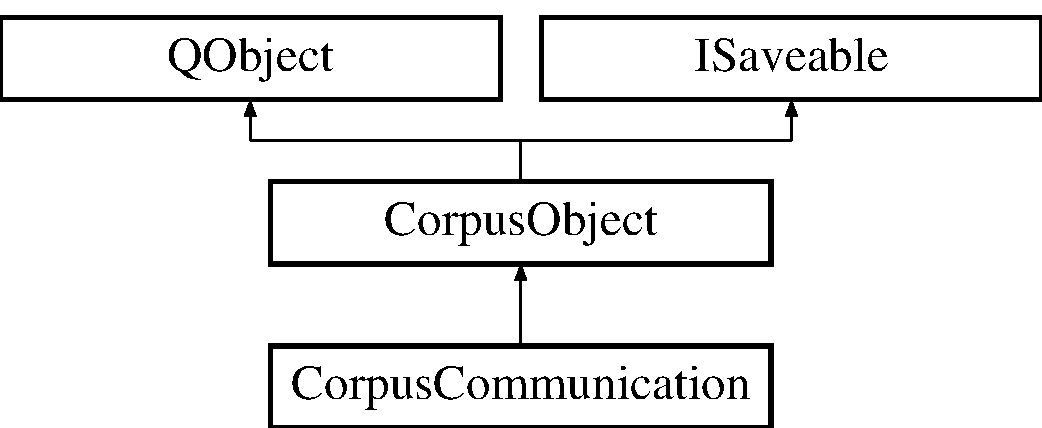
\includegraphics[height=3.000000cm]{class_corpus_communication}
\end{center}
\end{figure}
\subsection*{Signals}
\begin{DoxyCompactItemize}
\item 
\mbox{\Hypertarget{class_corpus_communication_a8048c2cd61bada85b866023c553dd32e}\label{class_corpus_communication_a8048c2cd61bada85b866023c553dd32e}} 
void {\bfseries corpus\+Recording\+Added} (Q\+Pointer$<$ P\+R\+A\+A\+L\+I\+N\+E\+\_\+\+C\+O\+R\+E\+\_\+\+N\+A\+M\+E\+S\+P\+A\+C\+E\+::\+Corpus\+Recording $>$ recording)
\item 
\mbox{\Hypertarget{class_corpus_communication_a696e92bbff3d1c317aee4c9cfb6bce9f}\label{class_corpus_communication_a696e92bbff3d1c317aee4c9cfb6bce9f}} 
void {\bfseries corpus\+Recording\+Deleted} (Q\+String communication\+ID, Q\+String recording\+ID)
\item 
\mbox{\Hypertarget{class_corpus_communication_a1eda96f1b582b8d7e4094b9a53faa587}\label{class_corpus_communication_a1eda96f1b582b8d7e4094b9a53faa587}} 
void {\bfseries corpus\+Annotation\+Added} (Q\+Pointer$<$ P\+R\+A\+A\+L\+I\+N\+E\+\_\+\+C\+O\+R\+E\+\_\+\+N\+A\+M\+E\+S\+P\+A\+C\+E\+::\+Corpus\+Annotation $>$ annotation)
\item 
\mbox{\Hypertarget{class_corpus_communication_a71c1c6deb1c74bf06d9fc15e78b174db}\label{class_corpus_communication_a71c1c6deb1c74bf06d9fc15e78b174db}} 
void {\bfseries corpus\+Annotation\+Deleted} (Q\+String communication\+ID, Q\+String annotation\+ID)
\end{DoxyCompactItemize}
\subsection*{Public Member Functions}
\begin{DoxyCompactItemize}
\item 
\mbox{\Hypertarget{class_corpus_communication_ad31f58fabee0a614ee124c3b795bc3ad}\label{class_corpus_communication_ad31f58fabee0a614ee124c3b795bc3ad}} 
{\bfseries Corpus\+Communication} (\hyperlink{class_corpus_repository}{Corpus\+Repository} $\ast$repository=nullptr, Q\+Object $\ast$parent=nullptr)
\item 
\mbox{\Hypertarget{class_corpus_communication_ae8e4b4e27772a2f65b0a6bdd90770d9a}\label{class_corpus_communication_ae8e4b4e27772a2f65b0a6bdd90770d9a}} 
{\bfseries Corpus\+Communication} (const Q\+String \&ID, \hyperlink{class_corpus_repository}{Corpus\+Repository} $\ast$repository=nullptr, Q\+Object $\ast$parent=nullptr)
\item 
\mbox{\Hypertarget{class_corpus_communication_a148919c92fd0bd530c02e21bc7b47cef}\label{class_corpus_communication_a148919c92fd0bd530c02e21bc7b47cef}} 
{\bfseries Corpus\+Communication} (\hyperlink{class_corpus_communication}{Corpus\+Communication} $\ast$other, Q\+Object $\ast$parent=nullptr)
\item 
\mbox{\Hypertarget{class_corpus_communication_aaf9f5021f355745621cc5b3723f97b88}\label{class_corpus_communication_aaf9f5021f355745621cc5b3723f97b88}} 
Corpus\+Object\+::\+Type {\bfseries type} () const override
\item 
\mbox{\Hypertarget{class_corpus_communication_a8a492d78bd3da6e73ff117af82aeeb7f}\label{class_corpus_communication_a8a492d78bd3da6e73ff117af82aeeb7f}} 
bool {\bfseries save} () override
\item 
\mbox{\Hypertarget{class_corpus_communication_a645454b2fd643c5cb276cdc89d6c0b44}\label{class_corpus_communication_a645454b2fd643c5cb276cdc89d6c0b44}} 
Q\+Pointer$<$ \hyperlink{class_corpus}{Corpus} $>$ {\bfseries corpus} () const
\item 
\mbox{\Hypertarget{class_corpus_communication_a6399e6c046291d2e2175044a98680b62}\label{class_corpus_communication_a6399e6c046291d2e2175044a98680b62}} 
Q\+String {\bfseries name} () const
\item 
\mbox{\Hypertarget{class_corpus_communication_a7cb8ac67e54fd08f8cfb7659cfe4df20}\label{class_corpus_communication_a7cb8ac67e54fd08f8cfb7659cfe4df20}} 
void {\bfseries set\+Name} (const Q\+String \&name)
\item 
\mbox{\Hypertarget{class_corpus_communication_af6cbf3648e853d94efc7181cd1a4f3eb}\label{class_corpus_communication_af6cbf3648e853d94efc7181cd1a4f3eb}} 
void {\bfseries set\+Corpus\+ID} (const Q\+String \&corpus\+ID) override
\item 
\mbox{\Hypertarget{class_corpus_communication_a35f2afa3731d8a0af46d34c7bff6bd6a}\label{class_corpus_communication_a35f2afa3731d8a0af46d34c7bff6bd6a}} 
Q\+Pointer$<$ \hyperlink{class_corpus_recording}{Corpus\+Recording} $>$ {\bfseries recording} (const Q\+String \&recording\+ID) const
\item 
\mbox{\Hypertarget{class_corpus_communication_a64898e8bf8c0802c40e847d54958fbe6}\label{class_corpus_communication_a64898e8bf8c0802c40e847d54958fbe6}} 
int {\bfseries recordings\+Count} () const
\item 
\mbox{\Hypertarget{class_corpus_communication_a1dc45504056a52c6dc20f3c8acc19809}\label{class_corpus_communication_a1dc45504056a52c6dc20f3c8acc19809}} 
bool {\bfseries has\+Recordings} () const
\item 
\mbox{\Hypertarget{class_corpus_communication_a7f77f4d7b4b130c31d6db5c1591230c0}\label{class_corpus_communication_a7f77f4d7b4b130c31d6db5c1591230c0}} 
bool {\bfseries has\+Recording} (const Q\+String \&recording\+ID) const
\item 
\mbox{\Hypertarget{class_corpus_communication_aaf2ef5dcc3594d1a24949f915cf23bfa}\label{class_corpus_communication_aaf2ef5dcc3594d1a24949f915cf23bfa}} 
const Q\+Map$<$ Q\+String, Q\+Pointer$<$ \hyperlink{class_corpus_recording}{Corpus\+Recording} $>$ $>$ \& {\bfseries recordings} () const
\item 
\mbox{\Hypertarget{class_corpus_communication_a7b752d1babaf38bf2dc29c7ca01a1f11}\label{class_corpus_communication_a7b752d1babaf38bf2dc29c7ca01a1f11}} 
Q\+List$<$ Q\+String $>$ {\bfseries recording\+I\+Ds} () const
\item 
\mbox{\Hypertarget{class_corpus_communication_adf43b6d6a4fce03cdd333a61346b543a}\label{class_corpus_communication_adf43b6d6a4fce03cdd333a61346b543a}} 
void {\bfseries add\+Recording} (\hyperlink{class_corpus_recording}{Corpus\+Recording} $\ast$recording)
\item 
\mbox{\Hypertarget{class_corpus_communication_ade2b822fd5a7029b05f08db3613f58be}\label{class_corpus_communication_ade2b822fd5a7029b05f08db3613f58be}} 
void {\bfseries remove\+Recording} (const Q\+String \&recording\+ID)
\item 
\mbox{\Hypertarget{class_corpus_communication_a4af937c3102c4a609214516dd4906893}\label{class_corpus_communication_a4af937c3102c4a609214516dd4906893}} 
double {\bfseries duration\+Sec} () const
\item 
\mbox{\Hypertarget{class_corpus_communication_a6e8c3fab9c1e84382613788afa1ad892}\label{class_corpus_communication_a6e8c3fab9c1e84382613788afa1ad892}} 
Q\+Pointer$<$ \hyperlink{class_corpus_annotation}{Corpus\+Annotation} $>$ {\bfseries annotation} (const Q\+String \&annotation\+ID) const
\item 
\mbox{\Hypertarget{class_corpus_communication_a97b5bf826b319808d100759d3b63daf1}\label{class_corpus_communication_a97b5bf826b319808d100759d3b63daf1}} 
int {\bfseries annotations\+Count} () const
\item 
\mbox{\Hypertarget{class_corpus_communication_aec4ab5d693d36a628a3ff3800a1cb2fa}\label{class_corpus_communication_aec4ab5d693d36a628a3ff3800a1cb2fa}} 
bool {\bfseries has\+Annotations} () const
\item 
\mbox{\Hypertarget{class_corpus_communication_a5de9631605419702088875b668b2ed4e}\label{class_corpus_communication_a5de9631605419702088875b668b2ed4e}} 
bool {\bfseries has\+Annotation} (const Q\+String \&annotation\+ID) const
\item 
\mbox{\Hypertarget{class_corpus_communication_a39033d3c365366cd7e687472187297bc}\label{class_corpus_communication_a39033d3c365366cd7e687472187297bc}} 
const Q\+Map$<$ Q\+String, Q\+Pointer$<$ \hyperlink{class_corpus_annotation}{Corpus\+Annotation} $>$ $>$ \& {\bfseries annotations} () const
\item 
\mbox{\Hypertarget{class_corpus_communication_a82456aa4a74824e65ca2c5607658871e}\label{class_corpus_communication_a82456aa4a74824e65ca2c5607658871e}} 
Q\+List$<$ Q\+String $>$ {\bfseries annotation\+I\+Ds} () const
\item 
\mbox{\Hypertarget{class_corpus_communication_a8761cb30f9108b257793c9035e71cbe2}\label{class_corpus_communication_a8761cb30f9108b257793c9035e71cbe2}} 
void {\bfseries add\+Annotation} (\hyperlink{class_corpus_annotation}{Corpus\+Annotation} $\ast$annotation)
\item 
\mbox{\Hypertarget{class_corpus_communication_a73cafc4b999510036f2e2417a51f25c8}\label{class_corpus_communication_a73cafc4b999510036f2e2417a51f25c8}} 
void {\bfseries remove\+Annotation} (const Q\+String \&annotation\+ID)
\end{DoxyCompactItemize}
\subsection*{Public Attributes}
\begin{DoxyCompactItemize}
\item 
\mbox{\Hypertarget{class_corpus_communication_a1a79b5e97057886b29ea41f1752f49ad}\label{class_corpus_communication_a1a79b5e97057886b29ea41f1752f49ad}} 
Q\+List$<$ Q\+String $>$ {\bfseries deleted\+Annotation\+I\+Ds}
\item 
\mbox{\Hypertarget{class_corpus_communication_a7ace8bca02f7247ae54dba95fb2024bd}\label{class_corpus_communication_a7ace8bca02f7247ae54dba95fb2024bd}} 
Q\+List$<$ Q\+String $>$ {\bfseries deleted\+Recording\+I\+Ds}
\end{DoxyCompactItemize}
\subsection*{Properties}
\begin{DoxyCompactItemize}
\item 
\mbox{\Hypertarget{class_corpus_communication_a1aeb5434de9c329b027618f77d707acf}\label{class_corpus_communication_a1aeb5434de9c329b027618f77d707acf}} 
Q\+String {\bfseries name}
\item 
\mbox{\Hypertarget{class_corpus_communication_a6e73b451bd9c76270e2de6294103bc6b}\label{class_corpus_communication_a6e73b451bd9c76270e2de6294103bc6b}} 
double {\bfseries duration\+Sec}
\end{DoxyCompactItemize}
\subsection*{Additional Inherited Members}


The documentation for this class was generated from the following files\+:\begin{DoxyCompactItemize}
\item 
/home/george/\+Develop/\+Praaline\+Py/praaline-\/core/corpus/Corpus\+Communication.\+h\item 
/home/george/\+Develop/\+Praaline\+Py/praaline-\/core/corpus/Corpus\+Communication.\+cpp\end{DoxyCompactItemize}

\hypertarget{class_corpus_datastore}{}\section{Corpus\+Datastore Class Reference}
\label{class_corpus_datastore}\index{Corpus\+Datastore@{Corpus\+Datastore}}
Inheritance diagram for Corpus\+Datastore\+:\begin{figure}[H]
\begin{center}
\leavevmode
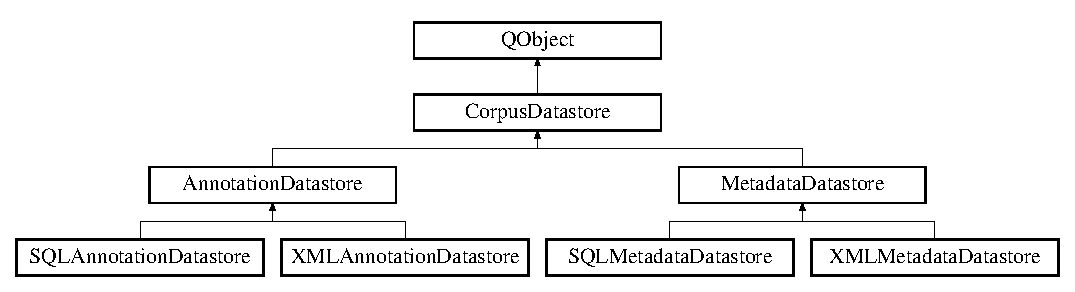
\includegraphics[height=3.478261cm]{class_corpus_datastore}
\end{center}
\end{figure}
\subsection*{Public Member Functions}
\begin{DoxyCompactItemize}
\item 
\mbox{\Hypertarget{class_corpus_datastore_ab203566a38835b0ddea25514316db6bf}\label{class_corpus_datastore_ab203566a38835b0ddea25514316db6bf}} 
{\bfseries Corpus\+Datastore} (\hyperlink{class_corpus_repository}{Corpus\+Repository} $\ast$repository, Q\+Object $\ast$parent=nullptr)
\item 
\mbox{\Hypertarget{class_corpus_datastore_a6a410cea025fa7fbbd74ab5b6449b4e7}\label{class_corpus_datastore_a6a410cea025fa7fbbd74ab5b6449b4e7}} 
void {\bfseries set\+Repository} (\hyperlink{class_corpus_object}{Corpus\+Object} $\ast$object)
\end{DoxyCompactItemize}
\subsection*{Protected Attributes}
\begin{DoxyCompactItemize}
\item 
\mbox{\Hypertarget{class_corpus_datastore_a035620fd72f93f9db363d9777b54adf8}\label{class_corpus_datastore_a035620fd72f93f9db363d9777b54adf8}} 
Q\+Pointer$<$ \hyperlink{class_corpus_repository}{Corpus\+Repository} $>$ {\bfseries m\+\_\+repository}
\end{DoxyCompactItemize}


The documentation for this class was generated from the following files\+:\begin{DoxyCompactItemize}
\item 
/home/george/\+Develop/\+Praaline\+Py/praaline-\/core/datastore/Corpus\+Datastore.\+h\item 
/home/george/\+Develop/\+Praaline\+Py/praaline-\/core/datastore/Corpus\+Datastore.\+cpp\end{DoxyCompactItemize}

\hypertarget{class_corpus_object}{}\section{Corpus\+Object Class Reference}
\label{class_corpus_object}\index{Corpus\+Object@{Corpus\+Object}}
Inheritance diagram for Corpus\+Object\+:\begin{figure}[H]
\begin{center}
\leavevmode
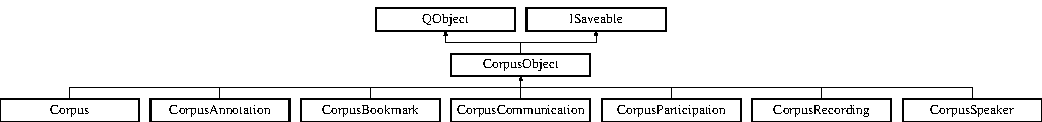
\includegraphics[height=1.643836cm]{class_corpus_object}
\end{center}
\end{figure}
\subsection*{Public Types}
\begin{DoxyCompactItemize}
\item 
\mbox{\Hypertarget{class_corpus_object_ab1f215448ffcef87c0c49aeef66db14a}\label{class_corpus_object_ab1f215448ffcef87c0c49aeef66db14a}} 
enum {\bfseries Type} \{ \newline
{\bfseries Type\+\_\+\+Corpus}, 
{\bfseries Type\+\_\+\+Communication}, 
{\bfseries Type\+\_\+\+Speaker}, 
{\bfseries Type\+\_\+\+Recording}, 
\newline
{\bfseries Type\+\_\+\+Annotation}, 
{\bfseries Type\+\_\+\+Participation}, 
{\bfseries Type\+\_\+\+Bookmark}, 
{\bfseries Type\+\_\+\+Undefined}
 \}
\end{DoxyCompactItemize}
\subsection*{Signals}
\begin{DoxyCompactItemize}
\item 
\mbox{\Hypertarget{class_corpus_object_aa2aa622291fe174695e2df7b3fe209f6}\label{class_corpus_object_aa2aa622291fe174695e2df7b3fe209f6}} 
void {\bfseries changed\+ID} (const Q\+String \&old\+ID, const Q\+String \&new\+ID)
\end{DoxyCompactItemize}
\subsection*{Public Member Functions}
\begin{DoxyCompactItemize}
\item 
\mbox{\Hypertarget{class_corpus_object_a566aa38d732176789207ea0d7fbab2bc}\label{class_corpus_object_a566aa38d732176789207ea0d7fbab2bc}} 
{\bfseries Corpus\+Object} (\hyperlink{class_corpus_repository}{Corpus\+Repository} $\ast$repository=nullptr, Q\+Object $\ast$parent=nullptr)
\item 
\mbox{\Hypertarget{class_corpus_object_a8e00309147ddefacf88b2d09e8727ec1}\label{class_corpus_object_a8e00309147ddefacf88b2d09e8727ec1}} 
{\bfseries Corpus\+Object} (const Q\+String \&ID, \hyperlink{class_corpus_repository}{Corpus\+Repository} $\ast$repository=nullptr, Q\+Object $\ast$parent=nullptr)
\item 
\mbox{\Hypertarget{class_corpus_object_a458418cb64b8605e7c2f7b7cdffa09ab}\label{class_corpus_object_a458418cb64b8605e7c2f7b7cdffa09ab}} 
virtual Q\+String {\bfseries ID} () const
\item 
\mbox{\Hypertarget{class_corpus_object_a05c01cd12ca002adda56391be2f13456}\label{class_corpus_object_a05c01cd12ca002adda56391be2f13456}} 
virtual void {\bfseries set\+ID} (const Q\+String \&ID)
\item 
\mbox{\Hypertarget{class_corpus_object_a7b738ad4e8eafe37d48b4e0b98f884f2}\label{class_corpus_object_a7b738ad4e8eafe37d48b4e0b98f884f2}} 
virtual Q\+String {\bfseries original\+ID} () const
\item 
\mbox{\Hypertarget{class_corpus_object_a37a6a4a4316fd90b3492cd483b0afc78}\label{class_corpus_object_a37a6a4a4316fd90b3492cd483b0afc78}} 
virtual Q\+String {\bfseries corpus\+ID} () const
\item 
\mbox{\Hypertarget{class_corpus_object_a8fc4da05cc682e58dd808fb74f1dd6df}\label{class_corpus_object_a8fc4da05cc682e58dd808fb74f1dd6df}} 
virtual void {\bfseries set\+Corpus\+ID} (const Q\+String \&corpus\+ID)
\item 
\mbox{\Hypertarget{class_corpus_object_a852a551d621797fa865826355b9949e8}\label{class_corpus_object_a852a551d621797fa865826355b9949e8}} 
virtual Corpus\+Object\+::\+Type {\bfseries type} () const =0
\item 
\mbox{\Hypertarget{class_corpus_object_aa703c47d513173a42d449a8896bc972d}\label{class_corpus_object_aa703c47d513173a42d449a8896bc972d}} 
virtual bool {\bfseries save} ()=0
\item 
\mbox{\Hypertarget{class_corpus_object_a373445edd8e454dbd4afe8e861f68243}\label{class_corpus_object_a373445edd8e454dbd4afe8e861f68243}} 
Q\+Variant {\bfseries property} (const Q\+String \&name) const
\item 
\mbox{\Hypertarget{class_corpus_object_a60216fe28daeecc9cb2fc30d38db3625}\label{class_corpus_object_a60216fe28daeecc9cb2fc30d38db3625}} 
bool {\bfseries set\+Property} (const Q\+String \&name, const Q\+Variant \&value)
\item 
\mbox{\Hypertarget{class_corpus_object_acf7d6ac282eb3a522ae37f8ee890fcef}\label{class_corpus_object_acf7d6ac282eb3a522ae37f8ee890fcef}} 
Q\+Pointer$<$ \hyperlink{class_corpus_repository}{Corpus\+Repository} $>$ {\bfseries repository} () const
\end{DoxyCompactItemize}
\subsection*{Static Public Member Functions}
\begin{DoxyCompactItemize}
\item 
\mbox{\Hypertarget{class_corpus_object_ae234a9c51d4835904f4266e333c85dd8}\label{class_corpus_object_ae234a9c51d4835904f4266e333c85dd8}} 
static Q\+String {\bfseries type\+To\+Friendly\+String} (Corpus\+Object\+::\+Type type)
\item 
\mbox{\Hypertarget{class_corpus_object_ac7e99e31de551e3af537963caf4584c7}\label{class_corpus_object_ac7e99e31de551e3af537963caf4584c7}} 
static Q\+String {\bfseries type\+To\+String} (Corpus\+Object\+::\+Type type)
\item 
\mbox{\Hypertarget{class_corpus_object_a25b56b17b6dcc2894c7590c3a43f9681}\label{class_corpus_object_a25b56b17b6dcc2894c7590c3a43f9681}} 
static Corpus\+Object\+::\+Type {\bfseries string\+To\+Type} (const Q\+String \&str)
\end{DoxyCompactItemize}
\subsection*{Protected Member Functions}
\begin{DoxyCompactItemize}
\item 
\mbox{\Hypertarget{class_corpus_object_a5e16a4a58de09340ba669bdea107b4d2}\label{class_corpus_object_a5e16a4a58de09340ba669bdea107b4d2}} 
void {\bfseries copy\+Properties\+From} (\hyperlink{class_corpus_object}{Corpus\+Object} $\ast$other)
\item 
\mbox{\Hypertarget{class_corpus_object_af91aaf99f39a8fc41ffbe62238c90c4e}\label{class_corpus_object_af91aaf99f39a8fc41ffbe62238c90c4e}} 
bool {\bfseries event\+Filter} (Q\+Object $\ast$obj, Q\+Event $\ast$event)
\end{DoxyCompactItemize}
\subsection*{Protected Attributes}
\begin{DoxyCompactItemize}
\item 
\mbox{\Hypertarget{class_corpus_object_a7c764f5c4ca06ae1910b90aaca70945a}\label{class_corpus_object_a7c764f5c4ca06ae1910b90aaca70945a}} 
Q\+String {\bfseries m\+\_\+\+ID}
\item 
\mbox{\Hypertarget{class_corpus_object_a31e6a6a19903610a4187aa0600dc0041}\label{class_corpus_object_a31e6a6a19903610a4187aa0600dc0041}} 
Q\+String {\bfseries m\+\_\+original\+ID}
\item 
\mbox{\Hypertarget{class_corpus_object_a00bfdb906e43b45e3d09f285d50d9007}\label{class_corpus_object_a00bfdb906e43b45e3d09f285d50d9007}} 
Q\+String {\bfseries m\+\_\+corpus\+ID}
\item 
\mbox{\Hypertarget{class_corpus_object_a5828ef6aeb1ae8277621786f22614c87}\label{class_corpus_object_a5828ef6aeb1ae8277621786f22614c87}} 
Q\+Pointer$<$ \hyperlink{class_corpus_repository}{Corpus\+Repository} $>$ {\bfseries m\+\_\+repository}
\end{DoxyCompactItemize}
\subsection*{Properties}
\begin{DoxyCompactItemize}
\item 
\mbox{\Hypertarget{class_corpus_object_a2e87f6afeb982f6b9ab31eb1f7423382}\label{class_corpus_object_a2e87f6afeb982f6b9ab31eb1f7423382}} 
Q\+String {\bfseries ID}
\item 
\mbox{\Hypertarget{class_corpus_object_aa54db2f97f4e244f229c2afbd26f8e34}\label{class_corpus_object_aa54db2f97f4e244f229c2afbd26f8e34}} 
Q\+String {\bfseries original\+ID}
\item 
\mbox{\Hypertarget{class_corpus_object_a580f7c90c3839b4b10bbac02a8b5b641}\label{class_corpus_object_a580f7c90c3839b4b10bbac02a8b5b641}} 
Q\+String {\bfseries corpus\+ID}
\item 
\mbox{\Hypertarget{class_corpus_object_a1eb66ea1ca76fcb8500ecf9b67959c66}\label{class_corpus_object_a1eb66ea1ca76fcb8500ecf9b67959c66}} 
Type {\bfseries type}
\end{DoxyCompactItemize}
\subsection*{Friends}
\begin{DoxyCompactItemize}
\item 
\mbox{\Hypertarget{class_corpus_object_a4fb3bed7506f0eb1a6ce3107c88f6561}\label{class_corpus_object_a4fb3bed7506f0eb1a6ce3107c88f6561}} 
class {\bfseries Corpus\+Datastore}
\end{DoxyCompactItemize}


The documentation for this class was generated from the following files\+:\begin{DoxyCompactItemize}
\item 
/home/george/\+Develop/\+Praaline\+Py/praaline-\/core/corpus/Corpus\+Object.\+h\item 
/home/george/\+Develop/\+Praaline\+Py/praaline-\/core/corpus/Corpus\+Object.\+cpp\end{DoxyCompactItemize}

\hypertarget{class_corpus_object_info}{}\section{Corpus\+Object\+Info Class Reference}
\label{class_corpus_object_info}\index{Corpus\+Object\+Info@{Corpus\+Object\+Info}}
Inheritance diagram for Corpus\+Object\+Info\+:\begin{figure}[H]
\begin{center}
\leavevmode
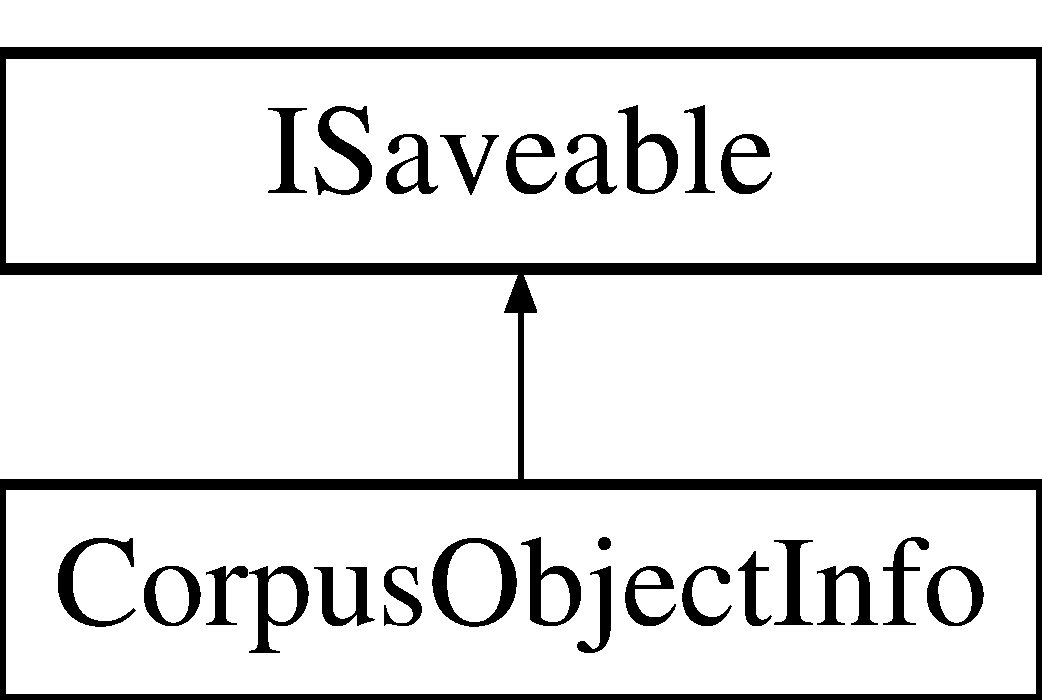
\includegraphics[height=2.000000cm]{class_corpus_object_info}
\end{center}
\end{figure}
\subsection*{Public Member Functions}
\begin{DoxyCompactItemize}
\item 
\mbox{\Hypertarget{class_corpus_object_info_a26f537cc34689b8ce4df14d57f0f81ba}\label{class_corpus_object_info_a26f537cc34689b8ce4df14d57f0f81ba}} 
{\bfseries Corpus\+Object\+Info} (Corpus\+Object\+::\+Type type)
\item 
\mbox{\Hypertarget{class_corpus_object_info_a5089ee69b35f30f00e103a487b0e970a}\label{class_corpus_object_info_a5089ee69b35f30f00e103a487b0e970a}} 
{\bfseries Corpus\+Object\+Info} (const \hyperlink{class_corpus_object_info}{Corpus\+Object\+Info} \&other)
\item 
\mbox{\Hypertarget{class_corpus_object_info_a451c0f8f88ee80a05abf7017cb6f2774}\label{class_corpus_object_info_a451c0f8f88ee80a05abf7017cb6f2774}} 
virtual Corpus\+Object\+::\+Type {\bfseries type} () const
\item 
\mbox{\Hypertarget{class_corpus_object_info_a273f644617e5df7213cad16c4849f564}\label{class_corpus_object_info_a273f644617e5df7213cad16c4849f564}} 
virtual Q\+Variant {\bfseries attribute} (const Q\+String \&name) const
\item 
\mbox{\Hypertarget{class_corpus_object_info_ad808b5e30083c42413c5c524fea19c23}\label{class_corpus_object_info_ad808b5e30083c42413c5c524fea19c23}} 
virtual void {\bfseries set\+Attribute} (const Q\+String \&name, Q\+Variant value)
\item 
\mbox{\Hypertarget{class_corpus_object_info_a2c4b752739540a1105fe1e89bc57f01e}\label{class_corpus_object_info_a2c4b752739540a1105fe1e89bc57f01e}} 
virtual const Q\+Variant\+Hash \& {\bfseries attributes} () const
\end{DoxyCompactItemize}
\subsection*{Friends}
\begin{DoxyCompactItemize}
\item 
\mbox{\Hypertarget{class_corpus_object_info_ad11ed9c2858f2dd5f875ff78f29d4875}\label{class_corpus_object_info_ad11ed9c2858f2dd5f875ff78f29d4875}} 
class {\bfseries Metadata\+Datastore}
\end{DoxyCompactItemize}
\subsection*{Additional Inherited Members}


The documentation for this class was generated from the following files\+:\begin{DoxyCompactItemize}
\item 
/home/george/\+Develop/\+Praaline\+Py/praaline-\/core/corpus/Corpus\+Object\+Info.\+h\item 
/home/george/\+Develop/\+Praaline\+Py/praaline-\/core/corpus/Corpus\+Object\+Info.\+cpp\end{DoxyCompactItemize}

\hypertarget{class_corpus_participation}{}\section{Corpus\+Participation Class Reference}
\label{class_corpus_participation}\index{Corpus\+Participation@{Corpus\+Participation}}
Inheritance diagram for Corpus\+Participation\+:\begin{figure}[H]
\begin{center}
\leavevmode
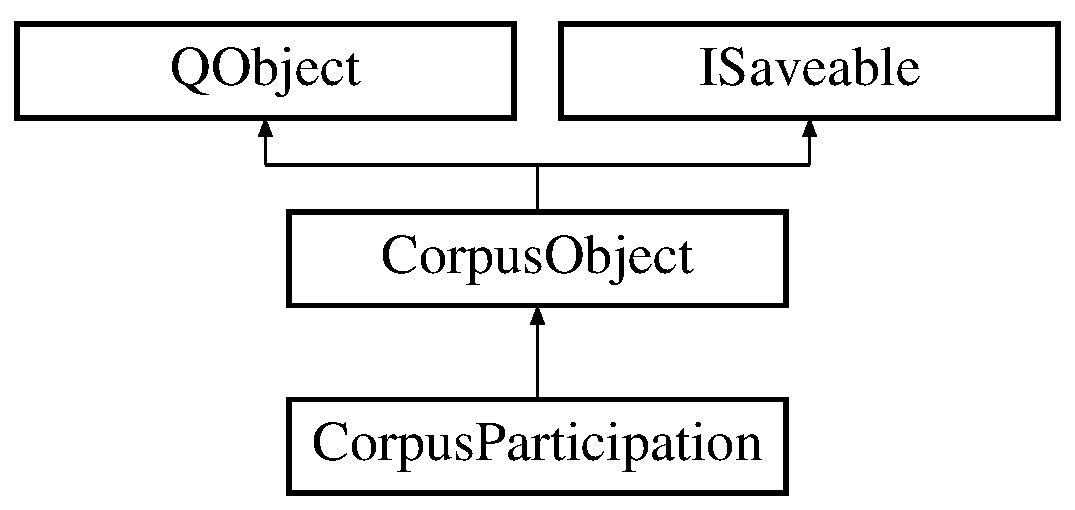
\includegraphics[height=3.000000cm]{class_corpus_participation}
\end{center}
\end{figure}
\subsection*{Public Member Functions}
\begin{DoxyCompactItemize}
\item 
\mbox{\Hypertarget{class_corpus_participation_a611cca39bda450b00bdd96931074e70e}\label{class_corpus_participation_a611cca39bda450b00bdd96931074e70e}} 
{\bfseries Corpus\+Participation} (Q\+Pointer$<$ \hyperlink{class_corpus_communication}{Corpus\+Communication} $>$ com, Q\+Pointer$<$ \hyperlink{class_corpus_speaker}{Corpus\+Speaker} $>$ spk, Q\+String role=Q\+String(), Q\+Object $\ast$parent=nullptr)
\item 
\mbox{\Hypertarget{class_corpus_participation_a3ed3ee7e6a624359ff65c6835053c33c}\label{class_corpus_participation_a3ed3ee7e6a624359ff65c6835053c33c}} 
void {\bfseries copy\+Properties} (\hyperlink{class_corpus_participation}{Corpus\+Participation} $\ast$other)
\item 
\mbox{\Hypertarget{class_corpus_participation_ad8d6762d4c75d24d8f2177195ed67ab6}\label{class_corpus_participation_ad8d6762d4c75d24d8f2177195ed67ab6}} 
Corpus\+Object\+::\+Type {\bfseries type} () const override
\item 
\mbox{\Hypertarget{class_corpus_participation_aee623d796afe4ca06b58612e33ed0fda}\label{class_corpus_participation_aee623d796afe4ca06b58612e33ed0fda}} 
bool {\bfseries save} () override
\item 
\mbox{\Hypertarget{class_corpus_participation_abc607ba572c0da844d19fca7b5c401ca}\label{class_corpus_participation_abc607ba572c0da844d19fca7b5c401ca}} 
Q\+String {\bfseries ID} () const override
\item 
\mbox{\Hypertarget{class_corpus_participation_a1de7ec05fe901de7eeeefd5430e333ce}\label{class_corpus_participation_a1de7ec05fe901de7eeeefd5430e333ce}} 
void {\bfseries set\+ID} (const Q\+String \&ID) override
\item 
\mbox{\Hypertarget{class_corpus_participation_aeae2f08284d743c43119f2fed9833529}\label{class_corpus_participation_aeae2f08284d743c43119f2fed9833529}} 
Q\+Pointer$<$ \hyperlink{class_corpus}{Corpus} $>$ {\bfseries corpus} () const
\item 
\mbox{\Hypertarget{class_corpus_participation_afb8e1d4dfc097d2b119e528119751de7}\label{class_corpus_participation_afb8e1d4dfc097d2b119e528119751de7}} 
Q\+Pointer$<$ \hyperlink{class_corpus_communication}{Corpus\+Communication} $>$ {\bfseries communication} () const
\item 
\mbox{\Hypertarget{class_corpus_participation_a1950c5466a90b664c752ff3573495322}\label{class_corpus_participation_a1950c5466a90b664c752ff3573495322}} 
Q\+Pointer$<$ \hyperlink{class_corpus_speaker}{Corpus\+Speaker} $>$ {\bfseries speaker} () const
\item 
\mbox{\Hypertarget{class_corpus_participation_a0af2fa63aa99ee59757c773b95f01114}\label{class_corpus_participation_a0af2fa63aa99ee59757c773b95f01114}} 
Q\+String {\bfseries communication\+ID} () const
\item 
\mbox{\Hypertarget{class_corpus_participation_a7b690bc0313ce0b951d05e46743e6c3a}\label{class_corpus_participation_a7b690bc0313ce0b951d05e46743e6c3a}} 
Q\+String {\bfseries speaker\+ID} () const
\item 
\mbox{\Hypertarget{class_corpus_participation_a295d64eae755449305efca0c81a6bdc7}\label{class_corpus_participation_a295d64eae755449305efca0c81a6bdc7}} 
Q\+String {\bfseries role} () const
\item 
\mbox{\Hypertarget{class_corpus_participation_ab511b1f01cabbfdb546d980d6267bf6b}\label{class_corpus_participation_ab511b1f01cabbfdb546d980d6267bf6b}} 
void {\bfseries set\+Role} (const Q\+String \&role)
\end{DoxyCompactItemize}
\subsection*{Properties}
\begin{DoxyCompactItemize}
\item 
\mbox{\Hypertarget{class_corpus_participation_a4fd5793010831cc4a61e940a5015116e}\label{class_corpus_participation_a4fd5793010831cc4a61e940a5015116e}} 
Q\+String {\bfseries communication\+ID}
\item 
\mbox{\Hypertarget{class_corpus_participation_a705af6c5979e4baa899e7c8c948bb39e}\label{class_corpus_participation_a705af6c5979e4baa899e7c8c948bb39e}} 
Q\+String {\bfseries speaker\+ID}
\item 
\mbox{\Hypertarget{class_corpus_participation_ac20d274dc5f43f1a14a3380bbc55e841}\label{class_corpus_participation_ac20d274dc5f43f1a14a3380bbc55e841}} 
Q\+String {\bfseries role}
\end{DoxyCompactItemize}
\subsection*{Additional Inherited Members}


The documentation for this class was generated from the following files\+:\begin{DoxyCompactItemize}
\item 
/home/george/\+Develop/\+Praaline\+Py/praaline-\/core/corpus/Corpus\+Participation.\+h\item 
/home/george/\+Develop/\+Praaline\+Py/praaline-\/core/corpus/Corpus\+Participation.\+cpp\end{DoxyCompactItemize}

\hypertarget{class_corpus_recording}{}\section{Corpus\+Recording Class Reference}
\label{class_corpus_recording}\index{Corpus\+Recording@{Corpus\+Recording}}
Inheritance diagram for Corpus\+Recording\+:\begin{figure}[H]
\begin{center}
\leavevmode
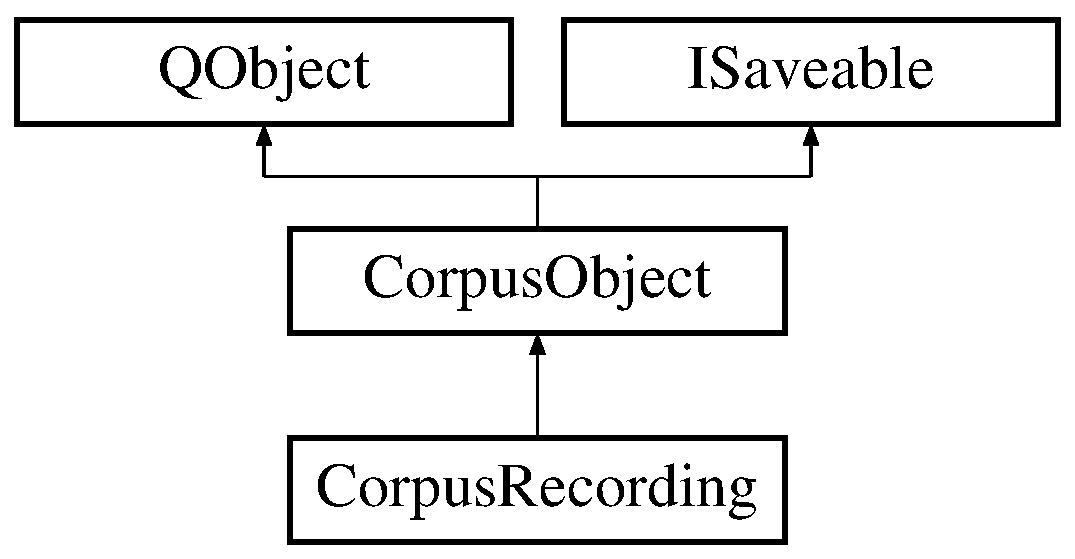
\includegraphics[height=3.000000cm]{class_corpus_recording}
\end{center}
\end{figure}
\subsection*{Public Member Functions}
\begin{DoxyCompactItemize}
\item 
\mbox{\Hypertarget{class_corpus_recording_a98f422ade47706ab47ed27ee6c31fbac}\label{class_corpus_recording_a98f422ade47706ab47ed27ee6c31fbac}} 
{\bfseries Corpus\+Recording} (\hyperlink{class_corpus_repository}{Corpus\+Repository} $\ast$repository=nullptr, Q\+Object $\ast$parent=nullptr)
\item 
\mbox{\Hypertarget{class_corpus_recording_a3e3502c3e982a42c8e60a15594b569c2}\label{class_corpus_recording_a3e3502c3e982a42c8e60a15594b569c2}} 
{\bfseries Corpus\+Recording} (const Q\+String ID, \hyperlink{class_corpus_repository}{Corpus\+Repository} $\ast$repository=nullptr, Q\+Object $\ast$parent=nullptr)
\item 
\mbox{\Hypertarget{class_corpus_recording_ad1364e9a6f224e418644bbacd9b1b36b}\label{class_corpus_recording_ad1364e9a6f224e418644bbacd9b1b36b}} 
{\bfseries Corpus\+Recording} (\hyperlink{class_corpus_recording}{Corpus\+Recording} $\ast$other, Q\+Object $\ast$parent=nullptr)
\item 
\mbox{\Hypertarget{class_corpus_recording_ac9a6a1406274c3dd36f0f562b531c522}\label{class_corpus_recording_ac9a6a1406274c3dd36f0f562b531c522}} 
Corpus\+Object\+::\+Type {\bfseries type} () const override
\item 
\mbox{\Hypertarget{class_corpus_recording_a9ce3f0e38c3a75e8ca229cf2df81ccb2}\label{class_corpus_recording_a9ce3f0e38c3a75e8ca229cf2df81ccb2}} 
bool {\bfseries save} () override
\item 
\mbox{\Hypertarget{class_corpus_recording_a443e8b8066600c9e6f0ed8a16a42e07e}\label{class_corpus_recording_a443e8b8066600c9e6f0ed8a16a42e07e}} 
Q\+String {\bfseries communication\+ID} () const
\item 
\mbox{\Hypertarget{class_corpus_recording_a256617f005a6bc4360b13b552f8dd642}\label{class_corpus_recording_a256617f005a6bc4360b13b552f8dd642}} 
Q\+Pointer$<$ \hyperlink{class_corpus}{Corpus} $>$ {\bfseries corpus} () const
\item 
\mbox{\Hypertarget{class_corpus_recording_a4336b3b38d50cc436e6bf5e434c14d08}\label{class_corpus_recording_a4336b3b38d50cc436e6bf5e434c14d08}} 
Q\+String {\bfseries base\+Path} () const
\item 
\mbox{\Hypertarget{class_corpus_recording_aa7d7f7139097301dd35e199e2ac3b505}\label{class_corpus_recording_aa7d7f7139097301dd35e199e2ac3b505}} 
Q\+String {\bfseries file\+Path} () const
\item 
\mbox{\Hypertarget{class_corpus_recording_a777e53057b4efeb5f193762519da9587}\label{class_corpus_recording_a777e53057b4efeb5f193762519da9587}} 
Q\+String {\bfseries name} () const
\item 
\mbox{\Hypertarget{class_corpus_recording_a67037b91f6f3c4b3b0364bc018c4a2a5}\label{class_corpus_recording_a67037b91f6f3c4b3b0364bc018c4a2a5}} 
void {\bfseries set\+Name} (const Q\+String \&name)
\item 
\mbox{\Hypertarget{class_corpus_recording_a4c569c78ba233dc501edd3b791805c5e}\label{class_corpus_recording_a4c569c78ba233dc501edd3b791805c5e}} 
Q\+String {\bfseries filename} () const
\item 
\mbox{\Hypertarget{class_corpus_recording_aa626693ea446a6d7a7f9534165e852e0}\label{class_corpus_recording_aa626693ea446a6d7a7f9534165e852e0}} 
void {\bfseries set\+Filename} (const Q\+String \&filename)
\item 
\mbox{\Hypertarget{class_corpus_recording_aa05f360593b3ea17024750a720cb3785}\label{class_corpus_recording_aa05f360593b3ea17024750a720cb3785}} 
Q\+String {\bfseries format} () const
\item 
\mbox{\Hypertarget{class_corpus_recording_a875f5a696ef8e90f3772010f584f58f2}\label{class_corpus_recording_a875f5a696ef8e90f3772010f584f58f2}} 
void {\bfseries set\+Format} (const Q\+String \&format)
\item 
\mbox{\Hypertarget{class_corpus_recording_acab3d304e1da2ad678def1a19bb33da1}\label{class_corpus_recording_acab3d304e1da2ad678def1a19bb33da1}} 
\hyperlink{struct_real_time}{Real\+Time} {\bfseries duration} () const
\item 
\mbox{\Hypertarget{class_corpus_recording_ac5b130acf20352407a2bf21a9ae9df77}\label{class_corpus_recording_ac5b130acf20352407a2bf21a9ae9df77}} 
void {\bfseries set\+Duration} (const \hyperlink{struct_real_time}{Real\+Time} \&duration)
\item 
\mbox{\Hypertarget{class_corpus_recording_a843221a0ccdc2960b4fc9e6c22cae7fd}\label{class_corpus_recording_a843221a0ccdc2960b4fc9e6c22cae7fd}} 
double {\bfseries duration\+Sec} () const
\item 
\mbox{\Hypertarget{class_corpus_recording_a9d7f07e7da9878b09dec5ed8a6bd5de9}\label{class_corpus_recording_a9d7f07e7da9878b09dec5ed8a6bd5de9}} 
void {\bfseries set\+Duration\+Sec} (double duration)
\item 
\mbox{\Hypertarget{class_corpus_recording_a3a5adeef9c4207f6d361a05ccf422954}\label{class_corpus_recording_a3a5adeef9c4207f6d361a05ccf422954}} 
int {\bfseries channels} () const
\item 
\mbox{\Hypertarget{class_corpus_recording_ae6d357b09f72910ba14b8ed42f364cba}\label{class_corpus_recording_ae6d357b09f72910ba14b8ed42f364cba}} 
void {\bfseries set\+Channels} (int channels)
\item 
\mbox{\Hypertarget{class_corpus_recording_a2eb1a4954a0cdf996a6a5c003d90af17}\label{class_corpus_recording_a2eb1a4954a0cdf996a6a5c003d90af17}} 
int {\bfseries sample\+Rate} () const
\item 
\mbox{\Hypertarget{class_corpus_recording_a3f88508e17242b42253ef283c34de558}\label{class_corpus_recording_a3f88508e17242b42253ef283c34de558}} 
void {\bfseries set\+Sample\+Rate} (int sample\+Rate)
\item 
\mbox{\Hypertarget{class_corpus_recording_acd4b8a16d8383ab6e9fc3955657b1e4d}\label{class_corpus_recording_acd4b8a16d8383ab6e9fc3955657b1e4d}} 
int {\bfseries precision\+Bits} () const
\item 
\mbox{\Hypertarget{class_corpus_recording_a8d414dc7f3175fb239cb53a9db1e6bc4}\label{class_corpus_recording_a8d414dc7f3175fb239cb53a9db1e6bc4}} 
void {\bfseries set\+Precision\+Bits} (int precision\+Bits)
\item 
\mbox{\Hypertarget{class_corpus_recording_a098e056795c73ef7e2e55b6ad423c8a1}\label{class_corpus_recording_a098e056795c73ef7e2e55b6ad423c8a1}} 
int {\bfseries bit\+Rate} () const
\item 
\mbox{\Hypertarget{class_corpus_recording_a0bce882cf34131dac826edf97177398d}\label{class_corpus_recording_a0bce882cf34131dac826edf97177398d}} 
void {\bfseries set\+Bit\+Rate} (int bit\+Rate)
\item 
\mbox{\Hypertarget{class_corpus_recording_a217854a9ac94194163275ae59395d9f5}\label{class_corpus_recording_a217854a9ac94194163275ae59395d9f5}} 
Q\+String {\bfseries encoding} () const
\item 
\mbox{\Hypertarget{class_corpus_recording_a4d785a2a267e2ccbd78d3a7fcf263343}\label{class_corpus_recording_a4d785a2a267e2ccbd78d3a7fcf263343}} 
void {\bfseries set\+Encoding} (const Q\+String \&encoding)
\item 
\mbox{\Hypertarget{class_corpus_recording_a072ad6cde836c102c0c3fce45b9edfa3}\label{class_corpus_recording_a072ad6cde836c102c0c3fce45b9edfa3}} 
long long {\bfseries file\+Size} () const
\item 
\mbox{\Hypertarget{class_corpus_recording_a4cb620a0f52f09719377a3443d27c000}\label{class_corpus_recording_a4cb620a0f52f09719377a3443d27c000}} 
void {\bfseries set\+File\+Size} (long long file\+Size)
\item 
\mbox{\Hypertarget{class_corpus_recording_ad35668b7ececf5593011ce786968ff47}\label{class_corpus_recording_ad35668b7ececf5593011ce786968ff47}} 
Q\+String {\bfseries checksum\+M\+D5} () const
\item 
\mbox{\Hypertarget{class_corpus_recording_ad08087038cfd7ed827a3bb8690c6d3dd}\label{class_corpus_recording_ad08087038cfd7ed827a3bb8690c6d3dd}} 
void {\bfseries set\+Checksum\+M\+D5} (const Q\+String \&checksum\+M\+D5)
\item 
\mbox{\Hypertarget{class_corpus_recording_af9df43d7255a8941658a34cdd3cc2133}\label{class_corpus_recording_af9df43d7255a8941658a34cdd3cc2133}} 
bool {\bfseries is\+File\+Available} () const
\item 
\mbox{\Hypertarget{class_corpus_recording_ad776aea49f4e694bb5c9c115d8176b58}\label{class_corpus_recording_ad776aea49f4e694bb5c9c115d8176b58}} 
Q\+Url {\bfseries media\+Url} () const
\end{DoxyCompactItemize}
\subsection*{Properties}
\begin{DoxyCompactItemize}
\item 
\mbox{\Hypertarget{class_corpus_recording_ac959e8535c7ec0656f3143c5dea8670c}\label{class_corpus_recording_ac959e8535c7ec0656f3143c5dea8670c}} 
Q\+String {\bfseries name}
\item 
\mbox{\Hypertarget{class_corpus_recording_a4b72515fb02737cd103d61da65e4315e}\label{class_corpus_recording_a4b72515fb02737cd103d61da65e4315e}} 
Q\+String {\bfseries filename}
\item 
\mbox{\Hypertarget{class_corpus_recording_a363517b572acd35fd7ff1c34a4e0b429}\label{class_corpus_recording_a363517b572acd35fd7ff1c34a4e0b429}} 
Q\+String {\bfseries format}
\item 
\mbox{\Hypertarget{class_corpus_recording_a9ced2cbd8e40e10adfcbfaaf79545d20}\label{class_corpus_recording_a9ced2cbd8e40e10adfcbfaaf79545d20}} 
double {\bfseries duration\+Sec}
\item 
\mbox{\Hypertarget{class_corpus_recording_ac69fe890614c9418db720b10c8b9af95}\label{class_corpus_recording_ac69fe890614c9418db720b10c8b9af95}} 
int {\bfseries channels}
\item 
\mbox{\Hypertarget{class_corpus_recording_a4cb468c16ad0d70f6c79157663b1fded}\label{class_corpus_recording_a4cb468c16ad0d70f6c79157663b1fded}} 
int {\bfseries sample\+Rate}
\item 
\mbox{\Hypertarget{class_corpus_recording_afbc0d8e7effb843f311b4fbdaf0bc26d}\label{class_corpus_recording_afbc0d8e7effb843f311b4fbdaf0bc26d}} 
int {\bfseries precision\+Bits}
\item 
\mbox{\Hypertarget{class_corpus_recording_a52e766751c464b546bc8cbd86fa0964d}\label{class_corpus_recording_a52e766751c464b546bc8cbd86fa0964d}} 
int {\bfseries bit\+Rate}
\item 
\mbox{\Hypertarget{class_corpus_recording_a37aee8b6a33abbdb0333373626bcf865}\label{class_corpus_recording_a37aee8b6a33abbdb0333373626bcf865}} 
Q\+String {\bfseries encoding}
\item 
\mbox{\Hypertarget{class_corpus_recording_a702ff000a0a9e291d2c8e602aee6e7a1}\label{class_corpus_recording_a702ff000a0a9e291d2c8e602aee6e7a1}} 
long long file\+Size {\bfseries R\+E\+AD}
\item 
\mbox{\Hypertarget{class_corpus_recording_a0e303f3e3ccc6f3c50f52459b0137e6d}\label{class_corpus_recording_a0e303f3e3ccc6f3c50f52459b0137e6d}} 
Q\+String {\bfseries checksum\+M\+D5}
\item 
\mbox{\Hypertarget{class_corpus_recording_a496a821357d804e9905d70aa8eed0ba5}\label{class_corpus_recording_a496a821357d804e9905d70aa8eed0ba5}} 
Q\+String {\bfseries communication\+ID}
\end{DoxyCompactItemize}
\subsection*{Additional Inherited Members}


The documentation for this class was generated from the following files\+:\begin{DoxyCompactItemize}
\item 
/home/george/\+Develop/\+Praaline\+Py/praaline-\/core/corpus/Corpus\+Recording.\+h\item 
/home/george/\+Develop/\+Praaline\+Py/praaline-\/core/corpus/Corpus\+Recording.\+cpp\end{DoxyCompactItemize}

\hypertarget{class_corpus_repository}{}\section{Corpus\+Repository Class Reference}
\label{class_corpus_repository}\index{Corpus\+Repository@{Corpus\+Repository}}
Inheritance diagram for Corpus\+Repository\+:\begin{figure}[H]
\begin{center}
\leavevmode
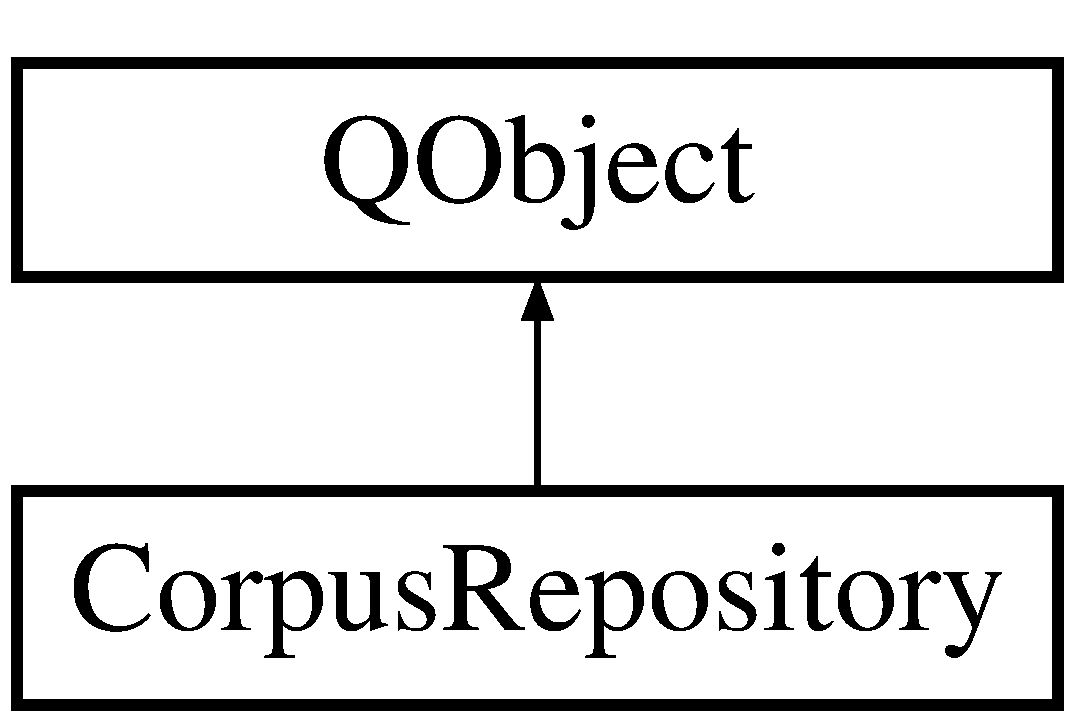
\includegraphics[height=2.000000cm]{class_corpus_repository}
\end{center}
\end{figure}
\subsection*{Signals}
\begin{DoxyCompactItemize}
\item 
\mbox{\Hypertarget{class_corpus_repository_a73d1198545d4557409620c1c361691bd}\label{class_corpus_repository_a73d1198545d4557409620c1c361691bd}} 
void {\bfseries changed\+ID} (const Q\+String \&old\+ID, const Q\+String \&new\+ID)
\item 
\mbox{\Hypertarget{class_corpus_repository_a46dca05e48d3b11613add7f8d18896c7}\label{class_corpus_repository_a46dca05e48d3b11613add7f8d18896c7}} 
void {\bfseries log\+Message} (const Q\+String \&category, const Q\+String \&message)
\end{DoxyCompactItemize}
\subsection*{Public Member Functions}
\begin{DoxyCompactItemize}
\item 
\mbox{\Hypertarget{class_corpus_repository_a9b505f5f200100ea4f2d77f55e7fc845}\label{class_corpus_repository_a9b505f5f200100ea4f2d77f55e7fc845}} 
void {\bfseries close} ()
\item 
\mbox{\Hypertarget{class_corpus_repository_ad2cc4235276a9255ba67685c97d5f051}\label{class_corpus_repository_ad2cc4235276a9255ba67685c97d5f051}} 
Q\+String {\bfseries ID} () const
\item 
\mbox{\Hypertarget{class_corpus_repository_a4039cf6526092b775f517dd297d8027b}\label{class_corpus_repository_a4039cf6526092b775f517dd297d8027b}} 
void {\bfseries set\+ID} (const Q\+String \&ID)
\item 
\mbox{\Hypertarget{class_corpus_repository_a145688e9ad7b25c86f9fc0d8cdd24be8}\label{class_corpus_repository_a145688e9ad7b25c86f9fc0d8cdd24be8}} 
Q\+String {\bfseries description} () const
\item 
\mbox{\Hypertarget{class_corpus_repository_a6c38e725b348fc1b0ff3430c0f20147f}\label{class_corpus_repository_a6c38e725b348fc1b0ff3430c0f20147f}} 
void {\bfseries set\+Description} (const Q\+String \&description)
\item 
\mbox{\Hypertarget{class_corpus_repository_ab0877cb895b6ce09361095cb34634556}\label{class_corpus_repository_ab0877cb895b6ce09361095cb34634556}} 
void {\bfseries set\+Base\+Path\+Media} (const Q\+String \&path)
\item 
\mbox{\Hypertarget{class_corpus_repository_a048c24879c8a9737ea5e863446016f03}\label{class_corpus_repository_a048c24879c8a9737ea5e863446016f03}} 
\hyperlink{class_corpus_repository_definition}{Corpus\+Repository\+Definition} {\bfseries definition} () const
\item 
\mbox{\Hypertarget{class_corpus_repository_a9a0a2c78a9bb86f4144d0a10ef6d3423}\label{class_corpus_repository_a9a0a2c78a9bb86f4144d0a10ef6d3423}} 
Q\+Pointer$<$ \hyperlink{class_annotation_datastore}{Annotation\+Datastore} $>$ {\bfseries annotations} () const
\item 
\mbox{\Hypertarget{class_corpus_repository_a58278c1281f30f1b7c94cacb21b9222a}\label{class_corpus_repository_a58278c1281f30f1b7c94cacb21b9222a}} 
Q\+Pointer$<$ \hyperlink{class_metadata_datastore}{Metadata\+Datastore} $>$ {\bfseries metadata} () const
\item 
\mbox{\Hypertarget{class_corpus_repository_af6cb68593edf8602a6f7beaa7809cad8}\label{class_corpus_repository_af6cb68593edf8602a6f7beaa7809cad8}} 
Q\+Pointer$<$ \hyperlink{class_file_datastore}{File\+Datastore} $>$ {\bfseries files} () const
\item 
\mbox{\Hypertarget{class_corpus_repository_a29b9720969815b8becd5f0febede876c}\label{class_corpus_repository_a29b9720969815b8becd5f0febede876c}} 
Q\+List$<$ \hyperlink{class_corpus_object_info}{Corpus\+Object\+Info} $>$ {\bfseries list\+Corpora\+Info} () const
\item 
\mbox{\Hypertarget{class_corpus_repository_abf2613f6bba1e93209523db15a258d9f}\label{class_corpus_repository_abf2613f6bba1e93209523db15a258d9f}} 
Q\+String\+List {\bfseries list\+Corpora\+I\+Ds} () const
\item 
\mbox{\Hypertarget{class_corpus_repository_a009752d30d8ab46a45b6936a7942aeb6}\label{class_corpus_repository_a009752d30d8ab46a45b6936a7942aeb6}} 
Q\+Pointer$<$ \hyperlink{class_metadata_structure}{Metadata\+Structure} $>$ {\bfseries metadata\+Structure} () const
\item 
\mbox{\Hypertarget{class_corpus_repository_a4036acd92e1c4c231fc6d14af0ab6efc}\label{class_corpus_repository_a4036acd92e1c4c231fc6d14af0ab6efc}} 
Q\+Pointer$<$ \hyperlink{class_annotation_structure}{Annotation\+Structure} $>$ {\bfseries annotation\+Structure} () const
\item 
\mbox{\Hypertarget{class_corpus_repository_a5b72d1398004a43d71609a8f7e03a9c2}\label{class_corpus_repository_a5b72d1398004a43d71609a8f7e03a9c2}} 
void {\bfseries import\+Metadata\+Structure} (\hyperlink{class_metadata_structure}{Metadata\+Structure} $\ast$other\+Structure)
\item 
\mbox{\Hypertarget{class_corpus_repository_ac087172e31a069907539d762fec9d830}\label{class_corpus_repository_ac087172e31a069907539d762fec9d830}} 
void {\bfseries import\+Annotation\+Structure} (\hyperlink{class_annotation_structure}{Annotation\+Structure} $\ast$other\+Structure)
\item 
\mbox{\Hypertarget{class_corpus_repository_a135593a4adab48ef03bc4106116020a2}\label{class_corpus_repository_a135593a4adab48ef03bc4106116020a2}} 
bool {\bfseries create\+Metadata\+Attribute} (Corpus\+Object\+::\+Type type, const Q\+String \&section\+ID, const Q\+String \&ID, const Q\+String \&name=Q\+String(), const Q\+String \&description=Q\+String(), const \hyperlink{class_data_type}{Data\+Type} \&datatype=\hyperlink{class_data_type}{Data\+Type}(\hyperlink{class_data_type_a8df455d8d3949b604fbb2967dfeff239a160c768176611f2649889e252c756539}{Data\+Type\+::\+Var\+Char}, 256), int order=0, bool indexed=false, const Q\+String \&name\+Value\+List=Q\+String())
\item 
\mbox{\Hypertarget{class_corpus_repository_a715e6a5c85b900be84f44b77763d9688}\label{class_corpus_repository_a715e6a5c85b900be84f44b77763d9688}} 
bool {\bfseries create\+Annotation\+Attribute} (const Q\+String \&annotation\+Level\+ID, const Q\+String \&ID, const Q\+String \&name=Q\+String(), const Q\+String \&description=Q\+String(), const \hyperlink{class_data_type}{Data\+Type} \&datatype=\hyperlink{class_data_type}{Data\+Type}(\hyperlink{class_data_type_a8df455d8d3949b604fbb2967dfeff239a160c768176611f2649889e252c756539}{Data\+Type\+::\+Var\+Char}, 256), int order=0, bool indexed=false, const Q\+String \&name\+Value\+List=Q\+String())
\item 
\mbox{\Hypertarget{class_corpus_repository_ae5455da3eed599d6a36dc1f4b082e141}\label{class_corpus_repository_ae5455da3eed599d6a36dc1f4b082e141}} 
Q\+String {\bfseries last\+Error} () const
\item 
\mbox{\Hypertarget{class_corpus_repository_a60314b693ebcf37904be5d5b911dcdcf}\label{class_corpus_repository_a60314b693ebcf37904be5d5b911dcdcf}} 
void {\bfseries set\+Last\+Error} (const Q\+String \&error\+Message)
\item 
\mbox{\Hypertarget{class_corpus_repository_a05b094b05a99c5b9360a8a4e36b465e7}\label{class_corpus_repository_a05b094b05a99c5b9360a8a4e36b465e7}} 
void {\bfseries clear\+Last\+Error} ()
\item 
\mbox{\Hypertarget{class_corpus_repository_a58ad4e9c09d31f9bfddcdaa833ffde6a}\label{class_corpus_repository_a58ad4e9c09d31f9bfddcdaa833ffde6a}} 
void {\bfseries send\+Log\+Message} (const Q\+String \&category, const Q\+String \&message)
\end{DoxyCompactItemize}
\subsection*{Static Public Member Functions}
\begin{DoxyCompactItemize}
\item 
\mbox{\Hypertarget{class_corpus_repository_a4306ac088c265f3d59f68c5357fcb078}\label{class_corpus_repository_a4306ac088c265f3d59f68c5357fcb078}} 
static \hyperlink{class_corpus_repository}{Corpus\+Repository} $\ast$ {\bfseries create} (const \hyperlink{class_corpus_repository_definition}{Corpus\+Repository\+Definition} \&definition, Q\+String \&error\+Messages, Q\+Object $\ast$parent=nullptr)
\item 
\mbox{\Hypertarget{class_corpus_repository_affb2746157b21a8ef2cd1de89e762814}\label{class_corpus_repository_affb2746157b21a8ef2cd1de89e762814}} 
static \hyperlink{class_corpus_repository}{Corpus\+Repository} $\ast$ {\bfseries open} (const \hyperlink{class_corpus_repository_definition}{Corpus\+Repository\+Definition} \&definition, Q\+String \&error\+Messages, Q\+Object $\ast$parent=nullptr)
\end{DoxyCompactItemize}


The documentation for this class was generated from the following files\+:\begin{DoxyCompactItemize}
\item 
/home/george/\+Develop/\+Praaline\+Py/praaline-\/core/datastore/Corpus\+Repository.\+h\item 
/home/george/\+Develop/\+Praaline\+Py/praaline-\/core/datastore/Corpus\+Repository.\+cpp\end{DoxyCompactItemize}

\hypertarget{struct_corpus_repository_data}{}\section{Corpus\+Repository\+Data Struct Reference}
\label{struct_corpus_repository_data}\index{Corpus\+Repository\+Data@{Corpus\+Repository\+Data}}
\subsection*{Public Attributes}
\begin{DoxyCompactItemize}
\item 
\mbox{\Hypertarget{struct_corpus_repository_data_ad2777c83efcf381505d50cc30b1a3fd8}\label{struct_corpus_repository_data_ad2777c83efcf381505d50cc30b1a3fd8}} 
\hyperlink{class_corpus_repository_definition}{Corpus\+Repository\+Definition} {\bfseries definition}
\item 
\mbox{\Hypertarget{struct_corpus_repository_data_af4509614c3d4290d5899db0487d00dee}\label{struct_corpus_repository_data_af4509614c3d4290d5899db0487d00dee}} 
Q\+Pointer$<$ \hyperlink{class_metadata_structure}{Metadata\+Structure} $>$ {\bfseries metadata\+Structure}
\item 
\mbox{\Hypertarget{struct_corpus_repository_data_a38f5d8938ab0cc6ce77823470b2d6dc0}\label{struct_corpus_repository_data_a38f5d8938ab0cc6ce77823470b2d6dc0}} 
Q\+Pointer$<$ \hyperlink{class_annotation_structure}{Annotation\+Structure} $>$ {\bfseries annotation\+Structure}
\item 
\mbox{\Hypertarget{struct_corpus_repository_data_a57e6849293f27d889108be91db99feeb}\label{struct_corpus_repository_data_a57e6849293f27d889108be91db99feeb}} 
Q\+Pointer$<$ \hyperlink{class_metadata_datastore}{Metadata\+Datastore} $>$ {\bfseries datastore\+Metadata}
\item 
\mbox{\Hypertarget{struct_corpus_repository_data_a609425de01cdd3dde351fb0963a48632}\label{struct_corpus_repository_data_a609425de01cdd3dde351fb0963a48632}} 
Q\+Pointer$<$ \hyperlink{class_annotation_datastore}{Annotation\+Datastore} $>$ {\bfseries datastore\+Annotations}
\item 
\mbox{\Hypertarget{struct_corpus_repository_data_abe4e1832acb4e0f8bf3d5ca8777bb478}\label{struct_corpus_repository_data_abe4e1832acb4e0f8bf3d5ca8777bb478}} 
Q\+Pointer$<$ \hyperlink{class_file_datastore}{File\+Datastore} $>$ {\bfseries datastore\+Files}
\item 
\mbox{\Hypertarget{struct_corpus_repository_data_a709b1a87f0891f5a8391d387e54291ae}\label{struct_corpus_repository_data_a709b1a87f0891f5a8391d387e54291ae}} 
Q\+String {\bfseries last\+Error}
\end{DoxyCompactItemize}


The documentation for this struct was generated from the following file\+:\begin{DoxyCompactItemize}
\item 
/home/george/\+Develop/\+Praaline\+Py/praaline-\/core/datastore/Corpus\+Repository.\+cpp\end{DoxyCompactItemize}

\hypertarget{class_corpus_repository_definition}{}\section{Corpus\+Repository\+Definition Class Reference}
\label{class_corpus_repository_definition}\index{Corpus\+Repository\+Definition@{Corpus\+Repository\+Definition}}
\subsection*{Public Member Functions}
\begin{DoxyCompactItemize}
\item 
\mbox{\Hypertarget{class_corpus_repository_definition_a7a5fdb5ca8899be3ea4a89ddabea3dda}\label{class_corpus_repository_definition_a7a5fdb5ca8899be3ea4a89ddabea3dda}} 
bool {\bfseries save} (const Q\+String \&filename)
\item 
\mbox{\Hypertarget{class_corpus_repository_definition_a298d1c7779aaca06b4298331d78214e1}\label{class_corpus_repository_definition_a298d1c7779aaca06b4298331d78214e1}} 
bool {\bfseries load} (const Q\+String \&filename)
\end{DoxyCompactItemize}
\subsection*{Public Attributes}
\begin{DoxyCompactItemize}
\item 
\mbox{\Hypertarget{class_corpus_repository_definition_a4ac448aed041a154050f249672b001c0}\label{class_corpus_repository_definition_a4ac448aed041a154050f249672b001c0}} 
Q\+String {\bfseries filename\+Definition}
\item 
\mbox{\Hypertarget{class_corpus_repository_definition_a811880cb773368317e6aab2245bc2a28}\label{class_corpus_repository_definition_a811880cb773368317e6aab2245bc2a28}} 
Q\+String {\bfseries repository\+ID}
\item 
\mbox{\Hypertarget{class_corpus_repository_definition_a5c6950346754c8a150230ac1ce237e0f}\label{class_corpus_repository_definition_a5c6950346754c8a150230ac1ce237e0f}} 
Q\+String {\bfseries repository\+Name}
\item 
\mbox{\Hypertarget{class_corpus_repository_definition_afc1f899f0de59297e36c52a8f757f831}\label{class_corpus_repository_definition_afc1f899f0de59297e36c52a8f757f831}} 
\hyperlink{class_datastore_info}{Datastore\+Info} {\bfseries info\+Datastore\+Metadata}
\item 
\mbox{\Hypertarget{class_corpus_repository_definition_ae1b4c80d3c6eb40e8c2ec0e8dbdd7d05}\label{class_corpus_repository_definition_ae1b4c80d3c6eb40e8c2ec0e8dbdd7d05}} 
\hyperlink{class_datastore_info}{Datastore\+Info} {\bfseries info\+Datastore\+Annotations}
\item 
\mbox{\Hypertarget{class_corpus_repository_definition_a6fc1aabd138c0645813d36c649e1a06c}\label{class_corpus_repository_definition_a6fc1aabd138c0645813d36c649e1a06c}} 
Q\+String {\bfseries base\+Path}
\item 
\mbox{\Hypertarget{class_corpus_repository_definition_abe0b1df1fddcc9b0ab8389af4f592784}\label{class_corpus_repository_definition_abe0b1df1fddcc9b0ab8389af4f592784}} 
Q\+String {\bfseries base\+Path\+Media}
\end{DoxyCompactItemize}


The documentation for this class was generated from the following files\+:\begin{DoxyCompactItemize}
\item 
/home/george/\+Develop/\+Praaline\+Py/praaline-\/core/datastore/Corpus\+Repository\+Definition.\+h\item 
/home/george/\+Develop/\+Praaline\+Py/praaline-\/core/datastore/Corpus\+Repository\+Definition.\+cpp\end{DoxyCompactItemize}

\hypertarget{class_corpus_speaker}{}\section{Corpus\+Speaker Class Reference}
\label{class_corpus_speaker}\index{Corpus\+Speaker@{Corpus\+Speaker}}
Inheritance diagram for Corpus\+Speaker\+:\begin{figure}[H]
\begin{center}
\leavevmode
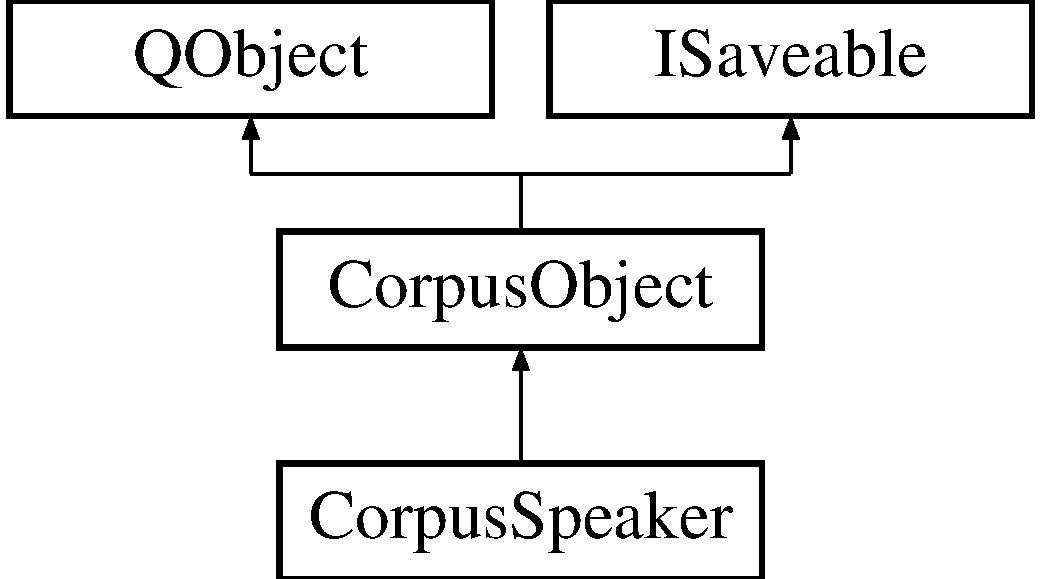
\includegraphics[height=3.000000cm]{class_corpus_speaker}
\end{center}
\end{figure}
\subsection*{Public Member Functions}
\begin{DoxyCompactItemize}
\item 
\mbox{\Hypertarget{class_corpus_speaker_ac6785e47e5c18dcb6a2e224bf2041e03}\label{class_corpus_speaker_ac6785e47e5c18dcb6a2e224bf2041e03}} 
{\bfseries Corpus\+Speaker} (\hyperlink{class_corpus_repository}{Corpus\+Repository} $\ast$repository=nullptr, Q\+Object $\ast$parent=nullptr)
\item 
\mbox{\Hypertarget{class_corpus_speaker_adaf34144e48ae95cc0e851230bd030e2}\label{class_corpus_speaker_adaf34144e48ae95cc0e851230bd030e2}} 
{\bfseries Corpus\+Speaker} (const Q\+String \&ID, \hyperlink{class_corpus_repository}{Corpus\+Repository} $\ast$repository=nullptr, Q\+Object $\ast$parent=nullptr)
\item 
\mbox{\Hypertarget{class_corpus_speaker_a8bc148ef6e1dd73b4d753ab6a7f46e03}\label{class_corpus_speaker_a8bc148ef6e1dd73b4d753ab6a7f46e03}} 
{\bfseries Corpus\+Speaker} (\hyperlink{class_corpus_speaker}{Corpus\+Speaker} $\ast$other, Q\+Object $\ast$parent=nullptr)
\item 
\mbox{\Hypertarget{class_corpus_speaker_ad047ccc247cb334b423ca53bd2f6fdfa}\label{class_corpus_speaker_ad047ccc247cb334b423ca53bd2f6fdfa}} 
Corpus\+Object\+::\+Type {\bfseries type} () const override
\item 
\mbox{\Hypertarget{class_corpus_speaker_ae8c6db0e0a36c7451b33e9d03bbb2314}\label{class_corpus_speaker_ae8c6db0e0a36c7451b33e9d03bbb2314}} 
bool {\bfseries save} () override
\item 
\mbox{\Hypertarget{class_corpus_speaker_a985fae57684965b1e57543828e7d2bef}\label{class_corpus_speaker_a985fae57684965b1e57543828e7d2bef}} 
Q\+Pointer$<$ \hyperlink{class_corpus}{Corpus} $>$ {\bfseries corpus} () const
\item 
\mbox{\Hypertarget{class_corpus_speaker_ab45ecf49db31a373de485010721e34f6}\label{class_corpus_speaker_ab45ecf49db31a373de485010721e34f6}} 
Q\+String {\bfseries name} () const
\item 
\mbox{\Hypertarget{class_corpus_speaker_aba787a3910c61d8a7ecee3547b0f98c6}\label{class_corpus_speaker_aba787a3910c61d8a7ecee3547b0f98c6}} 
void {\bfseries set\+Name} (const Q\+String \&name)
\end{DoxyCompactItemize}
\subsection*{Properties}
\begin{DoxyCompactItemize}
\item 
\mbox{\Hypertarget{class_corpus_speaker_a26ce91c653237ba60b54c2618727f54f}\label{class_corpus_speaker_a26ce91c653237ba60b54c2618727f54f}} 
Q\+String {\bfseries name}
\end{DoxyCompactItemize}
\subsection*{Additional Inherited Members}


The documentation for this class was generated from the following files\+:\begin{DoxyCompactItemize}
\item 
/home/george/\+Develop/\+Praaline\+Py/praaline-\/core/corpus/Corpus\+Speaker.\+h\item 
/home/george/\+Develop/\+Praaline\+Py/praaline-\/core/corpus/Corpus\+Speaker.\+cpp\end{DoxyCompactItemize}

\hypertarget{class_annotation_interface_praat_1_1_correspondance}{}\section{Annotation\+Interface\+Praat\+:\+:Correspondance Class Reference}
\label{class_annotation_interface_praat_1_1_correspondance}\index{Annotation\+Interface\+Praat\+::\+Correspondance@{Annotation\+Interface\+Praat\+::\+Correspondance}}
\subsection*{Public Member Functions}
\begin{DoxyCompactItemize}
\item 
\mbox{\Hypertarget{class_annotation_interface_praat_1_1_correspondance_a94a3546b1e06a49bf24685a8b4d96869}\label{class_annotation_interface_praat_1_1_correspondance_a94a3546b1e06a49bf24685a8b4d96869}} 
{\bfseries Correspondance} (const Q\+String \&level\+ID, const Q\+String \&attribute\+ID, const Q\+String \&tier\+Name)
\end{DoxyCompactItemize}
\subsection*{Public Attributes}
\begin{DoxyCompactItemize}
\item 
\mbox{\Hypertarget{class_annotation_interface_praat_1_1_correspondance_ad3521b5d25f28f8554f5e48d2a3fefe9}\label{class_annotation_interface_praat_1_1_correspondance_ad3521b5d25f28f8554f5e48d2a3fefe9}} 
Q\+String {\bfseries level\+ID}
\item 
\mbox{\Hypertarget{class_annotation_interface_praat_1_1_correspondance_af176c947a456e08bdd9f2636426400ce}\label{class_annotation_interface_praat_1_1_correspondance_af176c947a456e08bdd9f2636426400ce}} 
Q\+String {\bfseries attribute\+ID}
\item 
\mbox{\Hypertarget{class_annotation_interface_praat_1_1_correspondance_a1c123dbc9424ee99fc09bad0d9bf2a4a}\label{class_annotation_interface_praat_1_1_correspondance_a1c123dbc9424ee99fc09bad0d9bf2a4a}} 
Q\+String {\bfseries tier\+Name}
\end{DoxyCompactItemize}


The documentation for this class was generated from the following file\+:\begin{DoxyCompactItemize}
\item 
/home/george/\+Develop/\+Praaline\+Py/praaline-\/core/interfaces/praat/Annotation\+Interface\+Praat.\+h\end{DoxyCompactItemize}

\hypertarget{class_q_sql_migrator_1_1_commands_1_1_create_index}{}\section{Q\+Sql\+Migrator\+:\+:Commands\+:\+:Create\+Index Class Reference}
\label{class_q_sql_migrator_1_1_commands_1_1_create_index}\index{Q\+Sql\+Migrator\+::\+Commands\+::\+Create\+Index@{Q\+Sql\+Migrator\+::\+Commands\+::\+Create\+Index}}


value object representing the command to create an index  




{\ttfamily \#include $<$Create\+Index.\+h$>$}

Inheritance diagram for Q\+Sql\+Migrator\+:\+:Commands\+:\+:Create\+Index\+:\begin{figure}[H]
\begin{center}
\leavevmode
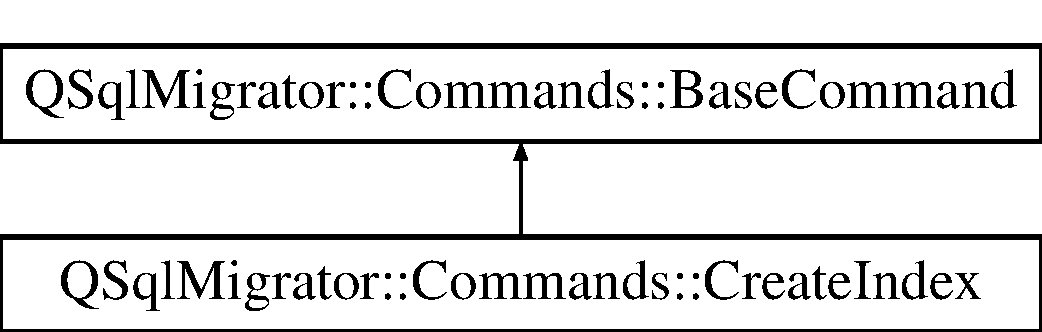
\includegraphics[height=2.000000cm]{class_q_sql_migrator_1_1_commands_1_1_create_index}
\end{center}
\end{figure}
\subsection*{Public Member Functions}
\begin{DoxyCompactItemize}
\item 
\mbox{\Hypertarget{class_q_sql_migrator_1_1_commands_1_1_create_index_abb648a593ac6fb23957eaf049b512401}\label{class_q_sql_migrator_1_1_commands_1_1_create_index_abb648a593ac6fb23957eaf049b512401}} 
{\bfseries Create\+Index} (const \hyperlink{class_q_sql_migrator_1_1_structure_1_1_index}{Structure\+::\+Index} \&index)
\item 
\mbox{\Hypertarget{class_q_sql_migrator_1_1_commands_1_1_create_index_a940f33d3b38dbe3ab5885a38beba9342}\label{class_q_sql_migrator_1_1_commands_1_1_create_index_a940f33d3b38dbe3ab5885a38beba9342}} 
const \hyperlink{class_q_sql_migrator_1_1_structure_1_1_index}{Structure\+::\+Index} \& {\bfseries index} () const
\item 
\mbox{\Hypertarget{class_q_sql_migrator_1_1_commands_1_1_create_index_a392c63c9a5af4864ee2ca62e4db36e3d}\label{class_q_sql_migrator_1_1_commands_1_1_create_index_a392c63c9a5af4864ee2ca62e4db36e3d}} 
Command\+Ptr {\bfseries reverse} () const Q\+\_\+\+D\+E\+C\+L\+\_\+\+O\+V\+E\+R\+R\+I\+DE
\end{DoxyCompactItemize}
\subsection*{Static Public Member Functions}
\begin{DoxyCompactItemize}
\item 
\mbox{\Hypertarget{class_q_sql_migrator_1_1_commands_1_1_create_index_a4563578789a966d217e4aeac1de517a1}\label{class_q_sql_migrator_1_1_commands_1_1_create_index_a4563578789a966d217e4aeac1de517a1}} 
static const Q\+String \& {\bfseries type\+Name} ()
\end{DoxyCompactItemize}


\subsection{Detailed Description}
value object representing the command to create an index 

The documentation for this class was generated from the following files\+:\begin{DoxyCompactItemize}
\item 
/home/george/\+Develop/\+Praaline\+Py/praaline-\/core/\+Q\+Sql\+Migrator/\+Commands/Create\+Index.\+h\item 
/home/george/\+Develop/\+Praaline\+Py/praaline-\/core/\+Q\+Sql\+Migrator/\+Commands/Create\+Index.\+cpp\end{DoxyCompactItemize}

\hypertarget{class_q_sql_migrator_1_1_commands_1_1_create_table}{}\section{Q\+Sql\+Migrator\+:\+:Commands\+:\+:Create\+Table Class Reference}
\label{class_q_sql_migrator_1_1_commands_1_1_create_table}\index{Q\+Sql\+Migrator\+::\+Commands\+::\+Create\+Table@{Q\+Sql\+Migrator\+::\+Commands\+::\+Create\+Table}}


value object representing the command to create a table  




{\ttfamily \#include $<$Create\+Table.\+h$>$}

Inheritance diagram for Q\+Sql\+Migrator\+:\+:Commands\+:\+:Create\+Table\+:\begin{figure}[H]
\begin{center}
\leavevmode
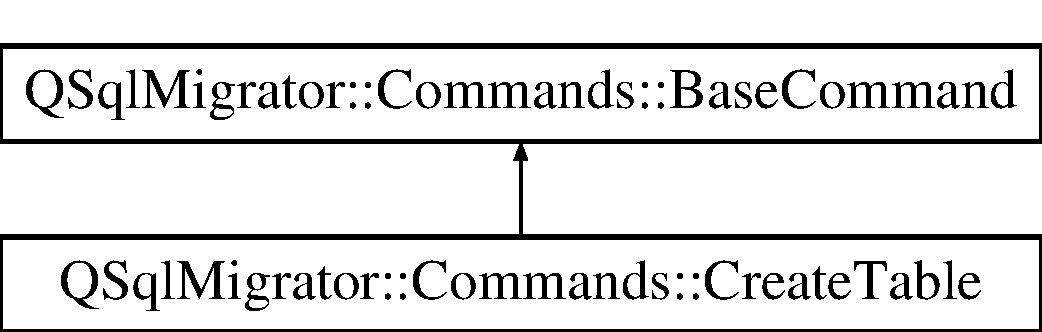
\includegraphics[height=2.000000cm]{class_q_sql_migrator_1_1_commands_1_1_create_table}
\end{center}
\end{figure}
\subsection*{Public Member Functions}
\begin{DoxyCompactItemize}
\item 
\mbox{\Hypertarget{class_q_sql_migrator_1_1_commands_1_1_create_table_a583435cb84744f93c2263c011ff2cdef}\label{class_q_sql_migrator_1_1_commands_1_1_create_table_a583435cb84744f93c2263c011ff2cdef}} 
{\bfseries Create\+Table} (const \hyperlink{class_q_sql_migrator_1_1_structure_1_1_table}{Structure\+::\+Table} \&table)
\item 
\mbox{\Hypertarget{class_q_sql_migrator_1_1_commands_1_1_create_table_a4ac559bfc140b2eb27e067a2aa18105a}\label{class_q_sql_migrator_1_1_commands_1_1_create_table_a4ac559bfc140b2eb27e067a2aa18105a}} 
const \hyperlink{class_q_sql_migrator_1_1_structure_1_1_table}{Structure\+::\+Table} \& {\bfseries table} () const
\item 
\mbox{\Hypertarget{class_q_sql_migrator_1_1_commands_1_1_create_table_acaf06336a0c7e0b195034cbb7a49f3e7}\label{class_q_sql_migrator_1_1_commands_1_1_create_table_acaf06336a0c7e0b195034cbb7a49f3e7}} 
Command\+Ptr {\bfseries reverse} () const Q\+\_\+\+D\+E\+C\+L\+\_\+\+O\+V\+E\+R\+R\+I\+DE
\end{DoxyCompactItemize}
\subsection*{Static Public Member Functions}
\begin{DoxyCompactItemize}
\item 
\mbox{\Hypertarget{class_q_sql_migrator_1_1_commands_1_1_create_table_a7859b0f3deac5e42d380b0b91a335024}\label{class_q_sql_migrator_1_1_commands_1_1_create_table_a7859b0f3deac5e42d380b0b91a335024}} 
static const Q\+String \& {\bfseries type\+Name} ()
\end{DoxyCompactItemize}


\subsection{Detailed Description}
value object representing the command to create a table 

The documentation for this class was generated from the following files\+:\begin{DoxyCompactItemize}
\item 
/home/george/\+Develop/\+Praaline\+Py/praaline-\/core/\+Q\+Sql\+Migrator/\+Commands/Create\+Table.\+h\item 
/home/george/\+Develop/\+Praaline\+Py/praaline-\/core/\+Q\+Sql\+Migrator/\+Commands/Create\+Table.\+cpp\end{DoxyCompactItemize}

\hypertarget{class_c_s_v_file_annotation}{}\section{C\+S\+V\+File\+Annotation Class Reference}
\label{class_c_s_v_file_annotation}\index{C\+S\+V\+File\+Annotation@{C\+S\+V\+File\+Annotation}}


The documentation for this class was generated from the following files\+:\begin{DoxyCompactItemize}
\item 
/home/george/\+Develop/\+Praaline\+Py/praaline-\/core/interfaces/csv/C\+S\+V\+File\+Annotation.\+h\item 
/home/george/\+Develop/\+Praaline\+Py/praaline-\/core/interfaces/csv/C\+S\+V\+File\+Annotation.\+cpp\end{DoxyCompactItemize}

\hypertarget{class_q_sql_migrator_1_1_commands_1_1_custom_command_base}{}\section{Q\+Sql\+Migrator\+:\+:Commands\+:\+:Custom\+Command\+Base Class Reference}
\label{class_q_sql_migrator_1_1_commands_1_1_custom_command_base}\index{Q\+Sql\+Migrator\+::\+Commands\+::\+Custom\+Command\+Base@{Q\+Sql\+Migrator\+::\+Commands\+::\+Custom\+Command\+Base}}


base class for custom commands  




{\ttfamily \#include $<$Custom\+Command\+Base.\+h$>$}

Inheritance diagram for Q\+Sql\+Migrator\+:\+:Commands\+:\+:Custom\+Command\+Base\+:\begin{figure}[H]
\begin{center}
\leavevmode
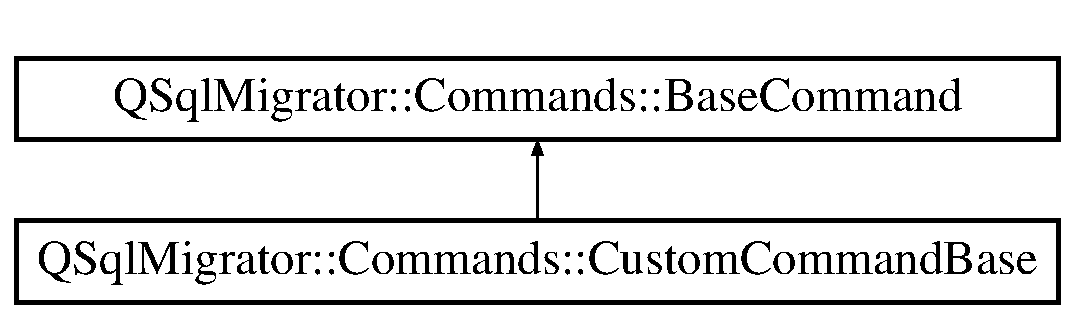
\includegraphics[height=2.000000cm]{class_q_sql_migrator_1_1_commands_1_1_custom_command_base}
\end{center}
\end{figure}
\subsection*{Public Member Functions}
\begin{DoxyCompactItemize}
\item 
\mbox{\Hypertarget{class_q_sql_migrator_1_1_commands_1_1_custom_command_base_a235261821273273feae5ae3b07eb75c0}\label{class_q_sql_migrator_1_1_commands_1_1_custom_command_base_a235261821273273feae5ae3b07eb75c0}} 
{\bfseries Custom\+Command\+Base} (const Q\+String \&command\+Name)
\item 
\mbox{\Hypertarget{class_q_sql_migrator_1_1_commands_1_1_custom_command_base_a15954460a6a5ba46757089f2b7ca6e32}\label{class_q_sql_migrator_1_1_commands_1_1_custom_command_base_a15954460a6a5ba46757089f2b7ca6e32}} 
const Q\+String \& {\bfseries custom\+Name} () const
\item 
\mbox{\Hypertarget{class_q_sql_migrator_1_1_commands_1_1_custom_command_base_ac2c8521957562d3e31ca4c95d008b641}\label{class_q_sql_migrator_1_1_commands_1_1_custom_command_base_ac2c8521957562d3e31ca4c95d008b641}} 
virtual bool {\bfseries up} (const Q\+Sql\+Database \&database) const =0
\item 
\mbox{\Hypertarget{class_q_sql_migrator_1_1_commands_1_1_custom_command_base_a76231dc0351ff7f4750a6f2411b30847}\label{class_q_sql_migrator_1_1_commands_1_1_custom_command_base_a76231dc0351ff7f4750a6f2411b30847}} 
virtual bool {\bfseries down} (const Q\+Sql\+Database \&database) const
\item 
Command\+Ptr \hyperlink{class_q_sql_migrator_1_1_commands_1_1_custom_command_base_a40c94f9cd360848f2c1c80b05a86ad08}{reverse} () const Q\+\_\+\+D\+E\+C\+L\+\_\+\+O\+V\+E\+R\+R\+I\+DE
\end{DoxyCompactItemize}
\subsection*{Static Public Member Functions}
\begin{DoxyCompactItemize}
\item 
\mbox{\Hypertarget{class_q_sql_migrator_1_1_commands_1_1_custom_command_base_adf2a577597d5d397ed15c95357aa1459}\label{class_q_sql_migrator_1_1_commands_1_1_custom_command_base_adf2a577597d5d397ed15c95357aa1459}} 
static const Q\+String \& {\bfseries type\+Name} ()
\end{DoxyCompactItemize}


\subsection{Detailed Description}
base class for custom commands 

\subsection{Member Function Documentation}
\mbox{\Hypertarget{class_q_sql_migrator_1_1_commands_1_1_custom_command_base_a40c94f9cd360848f2c1c80b05a86ad08}\label{class_q_sql_migrator_1_1_commands_1_1_custom_command_base_a40c94f9cd360848f2c1c80b05a86ad08}} 
\index{Q\+Sql\+Migrator\+::\+Commands\+::\+Custom\+Command\+Base@{Q\+Sql\+Migrator\+::\+Commands\+::\+Custom\+Command\+Base}!reverse@{reverse}}
\index{reverse@{reverse}!Q\+Sql\+Migrator\+::\+Commands\+::\+Custom\+Command\+Base@{Q\+Sql\+Migrator\+::\+Commands\+::\+Custom\+Command\+Base}}
\subsubsection{\texorpdfstring{reverse()}{reverse()}}
{\footnotesize\ttfamily Command\+Ptr Q\+Sql\+Migrator\+::\+Commands\+::\+Custom\+Command\+Base\+::reverse (\begin{DoxyParamCaption}{ }\end{DoxyParamCaption}) const\hspace{0.3cm}{\ttfamily [virtual]}}

\begin{DoxyReturn}{Returns}
invalid command (not reversable) 
\end{DoxyReturn}


Implements \hyperlink{class_q_sql_migrator_1_1_commands_1_1_base_command}{Q\+Sql\+Migrator\+::\+Commands\+::\+Base\+Command}.



The documentation for this class was generated from the following files\+:\begin{DoxyCompactItemize}
\item 
/home/george/\+Develop/\+Praaline\+Py/praaline-\/core/\+Q\+Sql\+Migrator/\+Commands/Custom\+Command\+Base.\+h\item 
/home/george/\+Develop/\+Praaline\+Py/praaline-\/core/\+Q\+Sql\+Migrator/\+Commands/Custom\+Command\+Base.\+cpp\end{DoxyCompactItemize}

\hypertarget{class_q_sql_migrator_1_1_command_execution_1_1_custom_command_service}{}\section{Q\+Sql\+Migrator\+:\+:Command\+Execution\+:\+:Custom\+Command\+Service Class Reference}
\label{class_q_sql_migrator_1_1_command_execution_1_1_custom_command_service}\index{Q\+Sql\+Migrator\+::\+Command\+Execution\+::\+Custom\+Command\+Service@{Q\+Sql\+Migrator\+::\+Command\+Execution\+::\+Custom\+Command\+Service}}
Inheritance diagram for Q\+Sql\+Migrator\+:\+:Command\+Execution\+:\+:Custom\+Command\+Service\+:\begin{figure}[H]
\begin{center}
\leavevmode
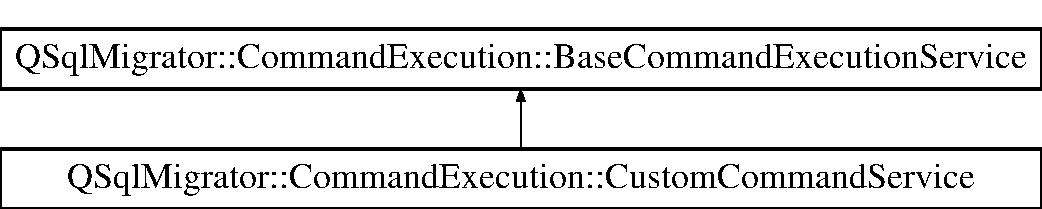
\includegraphics[height=2.000000cm]{class_q_sql_migrator_1_1_command_execution_1_1_custom_command_service}
\end{center}
\end{figure}
\subsection*{Public Member Functions}
\begin{DoxyCompactItemize}
\item 
\mbox{\Hypertarget{class_q_sql_migrator_1_1_command_execution_1_1_custom_command_service_a8c7a42129a19d3121fbfcc5d710b666d}\label{class_q_sql_migrator_1_1_command_execution_1_1_custom_command_service_a8c7a42129a19d3121fbfcc5d710b666d}} 
const Q\+String \& {\bfseries command\+Type} () const
\item 
\mbox{\Hypertarget{class_q_sql_migrator_1_1_command_execution_1_1_custom_command_service_a66b40615960798c7f31f351a88b9af7f}\label{class_q_sql_migrator_1_1_command_execution_1_1_custom_command_service_a66b40615960798c7f31f351a88b9af7f}} 
bool {\bfseries execute} (const Commands\+::\+Const\+Command\+Ptr \&command, \hyperlink{class_q_sql_migrator_1_1_command_execution_1_1_command_execution_context}{Command\+Execution\+::\+Command\+Execution\+Context} \&context) const
\item 
\mbox{\Hypertarget{class_q_sql_migrator_1_1_command_execution_1_1_custom_command_service_ace5d51ff7b7540280e6ad13e37320229}\label{class_q_sql_migrator_1_1_command_execution_1_1_custom_command_service_ace5d51ff7b7540280e6ad13e37320229}} 
bool {\bfseries is\+Valid} (const Commands\+::\+Const\+Command\+Ptr \&command, const \hyperlink{class_q_sql_migrator_1_1_command_execution_1_1_command_execution_context}{Command\+Execution\+::\+Command\+Execution\+Context} \&context) const
\item 
\mbox{\Hypertarget{class_q_sql_migrator_1_1_command_execution_1_1_custom_command_service_af785f29b6fc631ada9c4da6f2e234c81}\label{class_q_sql_migrator_1_1_command_execution_1_1_custom_command_service_af785f29b6fc631ada9c4da6f2e234c81}} 
bool {\bfseries down} (const Commands\+::\+Const\+Command\+Ptr \&command, \hyperlink{class_q_sql_migrator_1_1_command_execution_1_1_command_execution_context}{Command\+Execution\+::\+Command\+Execution\+Context} \&context) const
\item 
\mbox{\Hypertarget{class_q_sql_migrator_1_1_command_execution_1_1_custom_command_service_aa9921ce36db13f600d2509a46d9f00c9}\label{class_q_sql_migrator_1_1_command_execution_1_1_custom_command_service_aa9921ce36db13f600d2509a46d9f00c9}} 
bool {\bfseries is\+Down\+Valid} (const Commands\+::\+Const\+Command\+Ptr \&command, const \hyperlink{class_q_sql_migrator_1_1_command_execution_1_1_command_execution_context}{Command\+Execution\+::\+Command\+Execution\+Context} \&context) const
\end{DoxyCompactItemize}
\subsection*{Additional Inherited Members}


The documentation for this class was generated from the following files\+:\begin{DoxyCompactItemize}
\item 
/home/george/\+Develop/\+Praaline\+Py/praaline-\/core/\+Q\+Sql\+Migrator/\+Command\+Execution/Custom\+Command\+Service.\+h\item 
/home/george/\+Develop/\+Praaline\+Py/praaline-\/core/\+Q\+Sql\+Migrator/\+Command\+Execution/Custom\+Command\+Service.\+cpp\end{DoxyCompactItemize}

\hypertarget{class_q_sql_migrator_1_1_scheme_1_1_database}{}\section{Q\+Sql\+Migrator\+:\+:Scheme\+:\+:Database Class Reference}
\label{class_q_sql_migrator_1_1_scheme_1_1_database}\index{Q\+Sql\+Migrator\+::\+Scheme\+::\+Database@{Q\+Sql\+Migrator\+::\+Scheme\+::\+Database}}
\subsection*{Public Member Functions}
\begin{DoxyCompactItemize}
\item 
\mbox{\Hypertarget{class_q_sql_migrator_1_1_scheme_1_1_database_a171ce84b5baa23bda1ffd18ece0a282f}\label{class_q_sql_migrator_1_1_scheme_1_1_database_a171ce84b5baa23bda1ffd18ece0a282f}} 
\hyperlink{class_q_sql_migrator_1_1_scheme_1_1_database}{Database} \& {\bfseries operator$<$$<$} (const \hyperlink{class_q_sql_migrator_1_1_scheme_1_1_db_table}{Db\+Table} \&table)
\item 
\mbox{\Hypertarget{class_q_sql_migrator_1_1_scheme_1_1_database_a77ed29af79b49e042344b03e24c667ca}\label{class_q_sql_migrator_1_1_scheme_1_1_database_a77ed29af79b49e042344b03e24c667ca}} 
\hyperlink{class_q_sql_migrator_1_1_scheme_1_1_database}{Database} \& {\bfseries add} (const \hyperlink{class_q_sql_migrator_1_1_scheme_1_1_db_table}{Db\+Table} \&new\+Table)
\item 
\mbox{\Hypertarget{class_q_sql_migrator_1_1_scheme_1_1_database_aef366aceed0390f3a3e69415b9c5ebbf}\label{class_q_sql_migrator_1_1_scheme_1_1_database_aef366aceed0390f3a3e69415b9c5ebbf}} 
\hyperlink{class_q_sql_migrator_1_1_scheme_1_1_database}{Database} \& {\bfseries remove} (const \hyperlink{class_q_sql_migrator_1_1_scheme_1_1_db_table}{Db\+Table} \&table)
\item 
\mbox{\Hypertarget{class_q_sql_migrator_1_1_scheme_1_1_database_a2a7aaadbd7d94e76eed3527c48ce282d}\label{class_q_sql_migrator_1_1_scheme_1_1_database_a2a7aaadbd7d94e76eed3527c48ce282d}} 
\hyperlink{class_q_sql_migrator_1_1_scheme_1_1_database}{Database} \& {\bfseries remove\+Table} (const Q\+String \&table\+Name)
\end{DoxyCompactItemize}


The documentation for this class was generated from the following files\+:\begin{DoxyCompactItemize}
\item 
/home/george/\+Develop/\+Praaline\+Py/praaline-\/core/\+Q\+Sql\+Migrator/\+Scheme/Database.\+h\item 
/home/george/\+Develop/\+Praaline\+Py/praaline-\/core/\+Q\+Sql\+Migrator/\+Scheme/Database.\+cpp\end{DoxyCompactItemize}

\hypertarget{class_q_sql_migrator_1_1_sqlite_migrator_1_1_database_lock}{}\section{Q\+Sql\+Migrator\+:\+:Sqlite\+Migrator\+:\+:Database\+Lock Class Reference}
\label{class_q_sql_migrator_1_1_sqlite_migrator_1_1_database_lock}\index{Q\+Sql\+Migrator\+::\+Sqlite\+Migrator\+::\+Database\+Lock@{Q\+Sql\+Migrator\+::\+Sqlite\+Migrator\+::\+Database\+Lock}}


The \hyperlink{class_q_sql_migrator_1_1_sqlite_migrator_1_1_database_lock}{Database\+Lock} try to lock a database for this Q\+Sql\+Migrator process. You have to check if you got the lock ( see example with operator bool ).  




{\ttfamily \#include $<$Database\+Lock.\+h$>$}

Inheritance diagram for Q\+Sql\+Migrator\+:\+:Sqlite\+Migrator\+:\+:Database\+Lock\+:\begin{figure}[H]
\begin{center}
\leavevmode
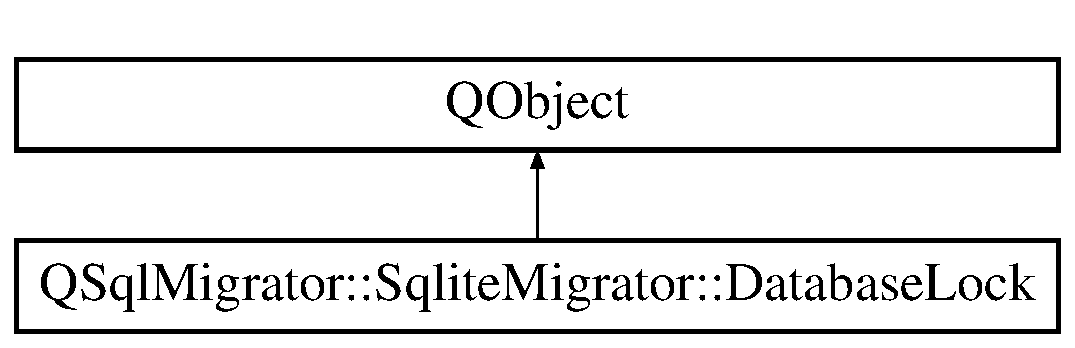
\includegraphics[height=2.000000cm]{class_q_sql_migrator_1_1_sqlite_migrator_1_1_database_lock}
\end{center}
\end{figure}
\subsection*{Public Member Functions}
\begin{DoxyCompactItemize}
\item 
\hyperlink{class_q_sql_migrator_1_1_sqlite_migrator_1_1_database_lock_abbbe7edb1c77fc3ed9a6a431b4d7cdcc}{Database\+Lock} (\hyperlink{class_q_sql_migrator_1_1_migration_execution_1_1_migration_execution_context}{Migration\+Execution\+::\+Migration\+Execution\+Context} \&context, unsigned int time\+Out\+Try\+Get\+Lock=time\+Out)
\item 
\hyperlink{class_q_sql_migrator_1_1_sqlite_migrator_1_1_database_lock_a42a41f79c57bea1253bea7794ad788ca}{operator bool} () const
\item 
\hyperlink{class_q_sql_migrator_1_1_sqlite_migrator_1_1_database_lock_ae8acecfef4f54eee37becd846fcff87a}{$\sim$\+Database\+Lock} ()
\end{DoxyCompactItemize}
\subsection*{Static Public Member Functions}
\begin{DoxyCompactItemize}
\item 
static Q\+String \hyperlink{class_q_sql_migrator_1_1_sqlite_migrator_1_1_database_lock_a77ec49dc6b304ebe0bdaada782eec6a6}{build\+Lock\+File\+Name} (const \hyperlink{class_q_sql_migrator_1_1_migration_execution_1_1_migration_execution_context}{Migration\+Execution\+::\+Migration\+Execution\+Context} \&context)
\end{DoxyCompactItemize}
\subsection*{Friends}
\begin{DoxyCompactItemize}
\item 
\mbox{\Hypertarget{class_q_sql_migrator_1_1_sqlite_migrator_1_1_database_lock_afe7f8ba95d43a7df07ee63e6f4e06926}\label{class_q_sql_migrator_1_1_sqlite_migrator_1_1_database_lock_afe7f8ba95d43a7df07ee63e6f4e06926}} 
class {\bfseries Refresh\+Lock\+Is\+Living\+Invoker}
\end{DoxyCompactItemize}


\subsection{Detailed Description}
The \hyperlink{class_q_sql_migrator_1_1_sqlite_migrator_1_1_database_lock}{Database\+Lock} try to lock a database for this Q\+Sql\+Migrator process. You have to check if you got the lock ( see example with operator bool ). 

The lock will be done with a lock-\/file in the same folder where the db is locatded.

The lock will automatically released on deconstruction.

Example\+:

unsigned int time\+Out\+To\+Get\+Lock = 60; context c( ... ); \hyperlink{class_q_sql_migrator_1_1_sqlite_migrator_1_1_database_lock}{Database\+Lock} lock(c, time\+Out\+To\+Get\+Lock); if(lock) \{ // do mirgration stuff \} 

\subsection{Constructor \& Destructor Documentation}
\mbox{\Hypertarget{class_q_sql_migrator_1_1_sqlite_migrator_1_1_database_lock_abbbe7edb1c77fc3ed9a6a431b4d7cdcc}\label{class_q_sql_migrator_1_1_sqlite_migrator_1_1_database_lock_abbbe7edb1c77fc3ed9a6a431b4d7cdcc}} 
\index{Q\+Sql\+Migrator\+::\+Sqlite\+Migrator\+::\+Database\+Lock@{Q\+Sql\+Migrator\+::\+Sqlite\+Migrator\+::\+Database\+Lock}!Database\+Lock@{Database\+Lock}}
\index{Database\+Lock@{Database\+Lock}!Q\+Sql\+Migrator\+::\+Sqlite\+Migrator\+::\+Database\+Lock@{Q\+Sql\+Migrator\+::\+Sqlite\+Migrator\+::\+Database\+Lock}}
\subsubsection{\texorpdfstring{Database\+Lock()}{DatabaseLock()}}
{\footnotesize\ttfamily Q\+Sql\+Migrator\+::\+Sqlite\+Migrator\+::\+Database\+Lock\+::\+Database\+Lock (\begin{DoxyParamCaption}\item[{\hyperlink{class_q_sql_migrator_1_1_migration_execution_1_1_migration_execution_context}{Migration\+Execution\+::\+Migration\+Execution\+Context} \&}]{context,  }\item[{unsigned int}]{time\+Out\+Try\+Get\+Lock = {\ttfamily timeOut} }\end{DoxyParamCaption})}

try to make a lock for the database in the context \mbox{\Hypertarget{class_q_sql_migrator_1_1_sqlite_migrator_1_1_database_lock_ae8acecfef4f54eee37becd846fcff87a}\label{class_q_sql_migrator_1_1_sqlite_migrator_1_1_database_lock_ae8acecfef4f54eee37becd846fcff87a}} 
\index{Q\+Sql\+Migrator\+::\+Sqlite\+Migrator\+::\+Database\+Lock@{Q\+Sql\+Migrator\+::\+Sqlite\+Migrator\+::\+Database\+Lock}!````~Database\+Lock@{$\sim$\+Database\+Lock}}
\index{````~Database\+Lock@{$\sim$\+Database\+Lock}!Q\+Sql\+Migrator\+::\+Sqlite\+Migrator\+::\+Database\+Lock@{Q\+Sql\+Migrator\+::\+Sqlite\+Migrator\+::\+Database\+Lock}}
\subsubsection{\texorpdfstring{$\sim$\+Database\+Lock()}{~DatabaseLock()}}
{\footnotesize\ttfamily Q\+Sql\+Migrator\+::\+Sqlite\+Migrator\+::\+Database\+Lock\+::$\sim$\+Database\+Lock (\begin{DoxyParamCaption}{ }\end{DoxyParamCaption})}

auto release the own lock 

\subsection{Member Function Documentation}
\mbox{\Hypertarget{class_q_sql_migrator_1_1_sqlite_migrator_1_1_database_lock_a77ec49dc6b304ebe0bdaada782eec6a6}\label{class_q_sql_migrator_1_1_sqlite_migrator_1_1_database_lock_a77ec49dc6b304ebe0bdaada782eec6a6}} 
\index{Q\+Sql\+Migrator\+::\+Sqlite\+Migrator\+::\+Database\+Lock@{Q\+Sql\+Migrator\+::\+Sqlite\+Migrator\+::\+Database\+Lock}!build\+Lock\+File\+Name@{build\+Lock\+File\+Name}}
\index{build\+Lock\+File\+Name@{build\+Lock\+File\+Name}!Q\+Sql\+Migrator\+::\+Sqlite\+Migrator\+::\+Database\+Lock@{Q\+Sql\+Migrator\+::\+Sqlite\+Migrator\+::\+Database\+Lock}}
\subsubsection{\texorpdfstring{build\+Lock\+File\+Name()}{buildLockFileName()}}
{\footnotesize\ttfamily Q\+String Q\+Sql\+Migrator\+::\+Sqlite\+Migrator\+::\+Database\+Lock\+::build\+Lock\+File\+Name (\begin{DoxyParamCaption}\item[{const \hyperlink{class_q_sql_migrator_1_1_migration_execution_1_1_migration_execution_context}{Migration\+Execution\+::\+Migration\+Execution\+Context} \&}]{context }\end{DoxyParamCaption})\hspace{0.3cm}{\ttfamily [static]}}

return the lock file name which will be used for this migration context \mbox{\Hypertarget{class_q_sql_migrator_1_1_sqlite_migrator_1_1_database_lock_a42a41f79c57bea1253bea7794ad788ca}\label{class_q_sql_migrator_1_1_sqlite_migrator_1_1_database_lock_a42a41f79c57bea1253bea7794ad788ca}} 
\index{Q\+Sql\+Migrator\+::\+Sqlite\+Migrator\+::\+Database\+Lock@{Q\+Sql\+Migrator\+::\+Sqlite\+Migrator\+::\+Database\+Lock}!operator bool@{operator bool}}
\index{operator bool@{operator bool}!Q\+Sql\+Migrator\+::\+Sqlite\+Migrator\+::\+Database\+Lock@{Q\+Sql\+Migrator\+::\+Sqlite\+Migrator\+::\+Database\+Lock}}
\subsubsection{\texorpdfstring{operator bool()}{operator bool()}}
{\footnotesize\ttfamily Q\+Sql\+Migrator\+::\+Sqlite\+Migrator\+::\+Database\+Lock\+::operator bool (\begin{DoxyParamCaption}{ }\end{DoxyParamCaption}) const}

return true if the lock is successfully set for this process 

The documentation for this class was generated from the following files\+:\begin{DoxyCompactItemize}
\item 
/home/george/\+Develop/\+Praaline\+Py/praaline-\/core/\+Q\+Sql\+Migrator/\+Databases/\+Sqlite\+Migrator/Database\+Lock.\+h\item 
/home/george/\+Develop/\+Praaline\+Py/praaline-\/core/\+Q\+Sql\+Migrator/\+Databases/\+Sqlite\+Migrator/Database\+Lock.\+cpp\end{DoxyCompactItemize}

\hypertarget{class_dataset}{}\section{Dataset Class Reference}
\label{class_dataset}\index{Dataset@{Dataset}}
\subsection*{Public Member Functions}
\begin{DoxyCompactItemize}
\item 
\mbox{\Hypertarget{class_dataset_a3ea4262e4c5f78c6c08892ec36154912}\label{class_dataset_a3ea4262e4c5f78c6c08892ec36154912}} 
void {\bfseries prepare} ()
\end{DoxyCompactItemize}


The documentation for this class was generated from the following files\+:\begin{DoxyCompactItemize}
\item 
/home/george/\+Develop/\+Praaline\+Py/praaline-\/core/query/Dataset.\+h\item 
/home/george/\+Develop/\+Praaline\+Py/praaline-\/core/query/Dataset.\+cpp\end{DoxyCompactItemize}

\hypertarget{class_dataset_definition}{}\section{Dataset\+Definition Class Reference}
\label{class_dataset_definition}\index{Dataset\+Definition@{Dataset\+Definition}}
\subsection*{Classes}
\begin{DoxyCompactItemize}
\item 
class \hyperlink{class_dataset_definition_1_1_column}{Column}
\end{DoxyCompactItemize}
\subsection*{Public Member Functions}
\begin{DoxyCompactItemize}
\item 
\mbox{\Hypertarget{class_dataset_definition_a9223d19e6a1aaf65bfaa13bec08fc4e3}\label{class_dataset_definition_a9223d19e6a1aaf65bfaa13bec08fc4e3}} 
Q\+String {\bfseries dataset\+Name} () const
\item 
\mbox{\Hypertarget{class_dataset_definition_a1dd20b6c722b1c5399be04e9d0361498}\label{class_dataset_definition_a1dd20b6c722b1c5399be04e9d0361498}} 
void {\bfseries set\+Dataset\+Name} (const Q\+String \&name)
\item 
\mbox{\Hypertarget{class_dataset_definition_aee848bad12756ef7115810fbd1b709a0}\label{class_dataset_definition_aee848bad12756ef7115810fbd1b709a0}} 
Q\+String {\bfseries minimal\+Level\+ID} () const
\item 
\mbox{\Hypertarget{class_dataset_definition_ac4e8fa3e80f34b081d902a8e9877daf2}\label{class_dataset_definition_ac4e8fa3e80f34b081d902a8e9877daf2}} 
void {\bfseries set\+Minimal\+Level\+ID} (const Q\+String \&level\+ID)
\item 
\mbox{\Hypertarget{class_dataset_definition_ab1ad323bfec8706f2a90f0336c293a98}\label{class_dataset_definition_ab1ad323bfec8706f2a90f0336c293a98}} 
Q\+List$<$ \hyperlink{class_dataset_definition_1_1_column}{Column} $>$ {\bfseries columns} () const
\item 
\mbox{\Hypertarget{class_dataset_definition_a19c88f8b5ffd35d58577ec58a24cc98f}\label{class_dataset_definition_a19c88f8b5ffd35d58577ec58a24cc98f}} 
\hyperlink{class_dataset_definition_1_1_column}{Column} {\bfseries column} (int index) const
\item 
\mbox{\Hypertarget{class_dataset_definition_aae7a5f778e90ae1dcde85e3e5aeb443a}\label{class_dataset_definition_aae7a5f778e90ae1dcde85e3e5aeb443a}} 
int {\bfseries column\+Count} () const
\item 
\mbox{\Hypertarget{class_dataset_definition_af4926f0eecf5ec5ff5a6dc3ef65f0752}\label{class_dataset_definition_af4926f0eecf5ec5ff5a6dc3ef65f0752}} 
void {\bfseries add\+Column} (const \hyperlink{class_dataset_definition_1_1_column}{Column} \&column)
\item 
\mbox{\Hypertarget{class_dataset_definition_a3a68d77df0e5af3e3e4a34116ebcfcd8}\label{class_dataset_definition_a3a68d77df0e5af3e3e4a34116ebcfcd8}} 
void {\bfseries add\+Columns} (const Q\+List$<$ \hyperlink{class_dataset_definition_1_1_column}{Column} $>$ \&columns)
\item 
\mbox{\Hypertarget{class_dataset_definition_a376dbf07084b0059cec161f05866e657}\label{class_dataset_definition_a376dbf07084b0059cec161f05866e657}} 
void {\bfseries remove\+Column} (int index)
\item 
\mbox{\Hypertarget{class_dataset_definition_a1287fda44b0a89e8f589a001a72dc8a7}\label{class_dataset_definition_a1287fda44b0a89e8f589a001a72dc8a7}} 
void {\bfseries clear} ()
\end{DoxyCompactItemize}


The documentation for this class was generated from the following files\+:\begin{DoxyCompactItemize}
\item 
/home/george/\+Develop/\+Praaline\+Py/praaline-\/core/query/Dataset\+Definition.\+h\item 
/home/george/\+Develop/\+Praaline\+Py/praaline-\/core/query/Dataset\+Definition.\+cpp\end{DoxyCompactItemize}

\hypertarget{struct_dataset_definition_data}{}\section{Dataset\+Definition\+Data Struct Reference}
\label{struct_dataset_definition_data}\index{Dataset\+Definition\+Data@{Dataset\+Definition\+Data}}
\subsection*{Public Attributes}
\begin{DoxyCompactItemize}
\item 
\mbox{\Hypertarget{struct_dataset_definition_data_ae02b36d39d6a7a33f9059613000f473d}\label{struct_dataset_definition_data_ae02b36d39d6a7a33f9059613000f473d}} 
Q\+String {\bfseries minimal\+Level\+ID}
\end{DoxyCompactItemize}


The documentation for this struct was generated from the following file\+:\begin{DoxyCompactItemize}
\item 
/home/george/\+Develop/\+Praaline\+Py/praaline-\/core/query/Dataset\+Definition.\+cpp\end{DoxyCompactItemize}

\hypertarget{class_datastore_factory}{}\section{Datastore\+Factory Class Reference}
\label{class_datastore_factory}\index{Datastore\+Factory@{Datastore\+Factory}}
\subsection*{Static Public Member Functions}
\begin{DoxyCompactItemize}
\item 
\mbox{\Hypertarget{class_datastore_factory_a59691abd37f28aac6c7f3b20f1360059}\label{class_datastore_factory_a59691abd37f28aac6c7f3b20f1360059}} 
static \hyperlink{class_annotation_datastore}{Annotation\+Datastore} $\ast$ {\bfseries get\+Annotation\+Datastore} (const \hyperlink{class_datastore_info}{Datastore\+Info} \&dsi, \hyperlink{class_annotation_structure}{Annotation\+Structure} $\ast$structure, \hyperlink{class_corpus_repository}{Corpus\+Repository} $\ast$repository)
\item 
\mbox{\Hypertarget{class_datastore_factory_a6763f50d61237fcfcd8d803c1dccead5}\label{class_datastore_factory_a6763f50d61237fcfcd8d803c1dccead5}} 
static \hyperlink{class_metadata_datastore}{Metadata\+Datastore} $\ast$ {\bfseries get\+Metadata\+Datastore} (const \hyperlink{class_datastore_info}{Datastore\+Info} \&dsi, \hyperlink{class_metadata_structure}{Metadata\+Structure} $\ast$structure, \hyperlink{class_corpus_repository}{Corpus\+Repository} $\ast$repository)
\end{DoxyCompactItemize}


The documentation for this class was generated from the following files\+:\begin{DoxyCompactItemize}
\item 
/home/george/\+Develop/\+Praaline\+Py/praaline-\/core/datastore/Datastore\+Factory.\+h\item 
/home/george/\+Develop/\+Praaline\+Py/praaline-\/core/datastore/Datastore\+Factory.\+cpp\end{DoxyCompactItemize}

\hypertarget{class_datastore_info}{}\section{Datastore\+Info Class Reference}
\label{class_datastore_info}\index{Datastore\+Info@{Datastore\+Info}}
\subsection*{Public Types}
\begin{DoxyCompactItemize}
\item 
\mbox{\Hypertarget{class_datastore_info_afdd306a952b938f923c0a6f0207d57d1}\label{class_datastore_info_afdd306a952b938f923c0a6f0207d57d1}} 
enum {\bfseries Type} \{ {\bfseries S\+QL}, 
{\bfseries X\+ML}, 
{\bfseries Files}
 \}
\end{DoxyCompactItemize}
\subsection*{Public Member Functions}
\begin{DoxyCompactItemize}
\item 
\mbox{\Hypertarget{class_datastore_info_aec3d52f4752cf57c4d7968d8e49b92f9}\label{class_datastore_info_aec3d52f4752cf57c4d7968d8e49b92f9}} 
{\bfseries Datastore\+Info} (Type type, Q\+String driver, Q\+String hostname, Q\+String datasource, Q\+String username, Q\+String password)
\item 
\mbox{\Hypertarget{class_datastore_info_a3ff5a103df525b8b87b3a52212205d34}\label{class_datastore_info_a3ff5a103df525b8b87b3a52212205d34}} 
Q\+String {\bfseries type\+To\+String} () const
\item 
\mbox{\Hypertarget{class_datastore_info_a8f39ec90621ad095f0ff14eab1de7352}\label{class_datastore_info_a8f39ec90621ad095f0ff14eab1de7352}} 
void {\bfseries set\+Type\+From\+String} (const Q\+String \&type\+String)
\end{DoxyCompactItemize}
\subsection*{Public Attributes}
\begin{DoxyCompactItemize}
\item 
\mbox{\Hypertarget{class_datastore_info_a58c34f47ef1a9ed785237aceb38fc01b}\label{class_datastore_info_a58c34f47ef1a9ed785237aceb38fc01b}} 
Type {\bfseries type}
\item 
\mbox{\Hypertarget{class_datastore_info_a6fd9cab603c209ecf7962b8e54273885}\label{class_datastore_info_a6fd9cab603c209ecf7962b8e54273885}} 
Q\+String {\bfseries driver}
\item 
\mbox{\Hypertarget{class_datastore_info_acc642a6098878b14cb3abab25b29f310}\label{class_datastore_info_acc642a6098878b14cb3abab25b29f310}} 
Q\+String {\bfseries hostname}
\item 
\mbox{\Hypertarget{class_datastore_info_a8153190b6af637fe6c0c9d5e87201b8b}\label{class_datastore_info_a8153190b6af637fe6c0c9d5e87201b8b}} 
Q\+String {\bfseries datasource}
\item 
\mbox{\Hypertarget{class_datastore_info_aa03e020c738ae76d94118e63c80ff48a}\label{class_datastore_info_aa03e020c738ae76d94118e63c80ff48a}} 
Q\+String {\bfseries username}
\item 
\mbox{\Hypertarget{class_datastore_info_a7c75852ff6d0e50d8a91a2fbb07224f9}\label{class_datastore_info_a7c75852ff6d0e50d8a91a2fbb07224f9}} 
Q\+String {\bfseries password}
\item 
\mbox{\Hypertarget{class_datastore_info_a35ed32b577354fadfe0140559908ffa7}\label{class_datastore_info_a35ed32b577354fadfe0140559908ffa7}} 
bool {\bfseries use\+Password}
\end{DoxyCompactItemize}


The documentation for this class was generated from the following file\+:\begin{DoxyCompactItemize}
\item 
/home/george/\+Develop/\+Praaline\+Py/praaline-\/core/datastore/Datastore\+Info.\+h\end{DoxyCompactItemize}

\hypertarget{class_data_type}{}\section{Data\+Type Class Reference}
\label{class_data_type}\index{Data\+Type@{Data\+Type}}


value object that represent any sql type  




{\ttfamily \#include $<$Data\+Type.\+h$>$}

\subsection*{Public Types}
\begin{DoxyCompactItemize}
\item 
enum \hyperlink{class_data_type_a8df455d8d3949b604fbb2967dfeff239}{Base} \{ \newline
{\bfseries Invalid}, 
\hyperlink{class_data_type_a8df455d8d3949b604fbb2967dfeff239a396f5ae6a2286ec8121a2146207850a5}{Char}, 
\hyperlink{class_data_type_a8df455d8d3949b604fbb2967dfeff239a160c768176611f2649889e252c756539}{Var\+Char}, 
\hyperlink{class_data_type_a8df455d8d3949b604fbb2967dfeff239ab4b13294ee3efac7e4831c55caa11022}{Binary}, 
\newline
\hyperlink{class_data_type_a8df455d8d3949b604fbb2967dfeff239a89f767813407ed2a706e8e8f69402667}{Var\+Binary}, 
{\bfseries Boolean}, 
\hyperlink{class_data_type_a8df455d8d3949b604fbb2967dfeff239a8d0497c1a18d35863fb81315b6d0bf41}{Small\+Int}, 
\hyperlink{class_data_type_a8df455d8d3949b604fbb2967dfeff239a3749547ad6302148b455bb3c0855689b}{Integer}, 
\newline
\hyperlink{class_data_type_a8df455d8d3949b604fbb2967dfeff239a4c9dd8d283c3f139832ae29d868fd79c}{Big\+Int}, 
\hyperlink{class_data_type_a8df455d8d3949b604fbb2967dfeff239a0e7950ea81022df1b093fd76fc773bcb}{Decimal}, 
{\bfseries Float}, 
{\bfseries Double}, 
\newline
{\bfseries Date}, 
{\bfseries Time}, 
{\bfseries Date\+Time}, 
{\bfseries Interval}, 
\newline
{\bfseries Array}, 
{\bfseries Multiset}, 
{\bfseries Xml}, 
{\bfseries Geometry}
 \}\begin{DoxyCompactList}\small\item\em Base Type enum. \end{DoxyCompactList}
\end{DoxyCompactItemize}
\subsection*{Public Member Functions}
\begin{DoxyCompactItemize}
\item 
\hyperlink{class_data_type_aa777acb36257198ce8db6d396fb94bb6}{Data\+Type} (const Q\+String \&\hyperlink{class_data_type_a61123733098ff8d26bef2a6a6401db83}{string})
\begin{DoxyCompactList}\small\item\em Construct the type from. \end{DoxyCompactList}\item 
\hyperlink{class_data_type_afe0f057e4b0556dd17cbefa59b2487dc}{Data\+Type} (\hyperlink{class_data_type_a8df455d8d3949b604fbb2967dfeff239}{Base} \hyperlink{class_data_type_ab74107f47a2a754eaf4b72e7b20e00d3}{base}, quint64 \hyperlink{class_data_type_a14a632d64fb970501b78c7b6f18d3ca7}{precision}=0, int \hyperlink{class_data_type_ad7bd76d9d549701b91bd9ede3dce889a}{scale}=0)
\begin{DoxyCompactList}\small\item\em Constructs the type. \end{DoxyCompactList}\item 
const Q\+String \hyperlink{class_data_type_a61123733098ff8d26bef2a6a6401db83}{string} () const
\item 
\hyperlink{class_data_type_a8df455d8d3949b604fbb2967dfeff239}{Base} \hyperlink{class_data_type_ab74107f47a2a754eaf4b72e7b20e00d3}{base} () const
\item 
quint64 \hyperlink{class_data_type_a14a632d64fb970501b78c7b6f18d3ca7}{precision} (quint64 default\+Value=0) const
\item 
int \hyperlink{class_data_type_ad7bd76d9d549701b91bd9ede3dce889a}{scale} () const
\item 
bool \hyperlink{class_data_type_ad7629e3562fdd2ad8afea12050dec31b}{is\+Valid} () const
\end{DoxyCompactItemize}
\subsection*{Static Public Member Functions}
\begin{DoxyCompactItemize}
\item 
static const \hyperlink{class_data_type}{Data\+Type} \& \hyperlink{class_data_type_a57b17d24ef05c53131e20dfcd54e219d}{invalid} ()
\end{DoxyCompactItemize}


\subsection{Detailed Description}
value object that represent any sql type 

\subsection{Member Enumeration Documentation}
\mbox{\Hypertarget{class_data_type_a8df455d8d3949b604fbb2967dfeff239}\label{class_data_type_a8df455d8d3949b604fbb2967dfeff239}} 
\index{Data\+Type@{Data\+Type}!Base@{Base}}
\index{Base@{Base}!Data\+Type@{Data\+Type}}
\subsubsection{\texorpdfstring{Base}{Base}}
{\footnotesize\ttfamily enum \hyperlink{class_data_type_a8df455d8d3949b604fbb2967dfeff239}{Data\+Type\+::\+Base}}



Base Type enum. 

\begin{DoxyEnumFields}{Enumerator}
\raisebox{\heightof{T}}[0pt][0pt]{\index{Char@{Char}!Data\+Type@{Data\+Type}}\index{Data\+Type@{Data\+Type}!Char@{Char}}}\mbox{\Hypertarget{class_data_type_a8df455d8d3949b604fbb2967dfeff239a396f5ae6a2286ec8121a2146207850a5}\label{class_data_type_a8df455d8d3949b604fbb2967dfeff239a396f5ae6a2286ec8121a2146207850a5}} 
Char&precision is length (defaults to 1) \\
\hline

\raisebox{\heightof{T}}[0pt][0pt]{\index{Var\+Char@{Var\+Char}!Data\+Type@{Data\+Type}}\index{Data\+Type@{Data\+Type}!Var\+Char@{Var\+Char}}}\mbox{\Hypertarget{class_data_type_a8df455d8d3949b604fbb2967dfeff239a160c768176611f2649889e252c756539}\label{class_data_type_a8df455d8d3949b604fbb2967dfeff239a160c768176611f2649889e252c756539}} 
Var\+Char&precision is maximum length (defaults to 255) \\
\hline

\raisebox{\heightof{T}}[0pt][0pt]{\index{Binary@{Binary}!Data\+Type@{Data\+Type}}\index{Data\+Type@{Data\+Type}!Binary@{Binary}}}\mbox{\Hypertarget{class_data_type_a8df455d8d3949b604fbb2967dfeff239ab4b13294ee3efac7e4831c55caa11022}\label{class_data_type_a8df455d8d3949b604fbb2967dfeff239ab4b13294ee3efac7e4831c55caa11022}} 
Binary&precision represents length in bytes (required) \\
\hline

\raisebox{\heightof{T}}[0pt][0pt]{\index{Var\+Binary@{Var\+Binary}!Data\+Type@{Data\+Type}}\index{Data\+Type@{Data\+Type}!Var\+Binary@{Var\+Binary}}}\mbox{\Hypertarget{class_data_type_a8df455d8d3949b604fbb2967dfeff239a89f767813407ed2a706e8e8f69402667}\label{class_data_type_a8df455d8d3949b604fbb2967dfeff239a89f767813407ed2a706e8e8f69402667}} 
Var\+Binary&precision represents maximum bytes \\
\hline

\raisebox{\heightof{T}}[0pt][0pt]{\index{Small\+Int@{Small\+Int}!Data\+Type@{Data\+Type}}\index{Data\+Type@{Data\+Type}!Small\+Int@{Small\+Int}}}\mbox{\Hypertarget{class_data_type_a8df455d8d3949b604fbb2967dfeff239a8d0497c1a18d35863fb81315b6d0bf41}\label{class_data_type_a8df455d8d3949b604fbb2967dfeff239a8d0497c1a18d35863fb81315b6d0bf41}} 
Small\+Int&precision is 5 \\
\hline

\raisebox{\heightof{T}}[0pt][0pt]{\index{Integer@{Integer}!Data\+Type@{Data\+Type}}\index{Data\+Type@{Data\+Type}!Integer@{Integer}}}\mbox{\Hypertarget{class_data_type_a8df455d8d3949b604fbb2967dfeff239a3749547ad6302148b455bb3c0855689b}\label{class_data_type_a8df455d8d3949b604fbb2967dfeff239a3749547ad6302148b455bb3c0855689b}} 
Integer&precision defaults to 10 \\
\hline

\raisebox{\heightof{T}}[0pt][0pt]{\index{Big\+Int@{Big\+Int}!Data\+Type@{Data\+Type}}\index{Data\+Type@{Data\+Type}!Big\+Int@{Big\+Int}}}\mbox{\Hypertarget{class_data_type_a8df455d8d3949b604fbb2967dfeff239a4c9dd8d283c3f139832ae29d868fd79c}\label{class_data_type_a8df455d8d3949b604fbb2967dfeff239a4c9dd8d283c3f139832ae29d868fd79c}} 
Big\+Int&precision is 19 \\
\hline

\raisebox{\heightof{T}}[0pt][0pt]{\index{Decimal@{Decimal}!Data\+Type@{Data\+Type}}\index{Data\+Type@{Data\+Type}!Decimal@{Decimal}}}\mbox{\Hypertarget{class_data_type_a8df455d8d3949b604fbb2967dfeff239a0e7950ea81022df1b093fd76fc773bcb}\label{class_data_type_a8df455d8d3949b604fbb2967dfeff239a0e7950ea81022df1b093fd76fc773bcb}} 
Decimal&precision and scale required (total digits, digits after comma) \\
\hline

\end{DoxyEnumFields}


\subsection{Constructor \& Destructor Documentation}
\mbox{\Hypertarget{class_data_type_aa777acb36257198ce8db6d396fb94bb6}\label{class_data_type_aa777acb36257198ce8db6d396fb94bb6}} 
\index{Data\+Type@{Data\+Type}!Data\+Type@{Data\+Type}}
\index{Data\+Type@{Data\+Type}!Data\+Type@{Data\+Type}}
\subsubsection{\texorpdfstring{Data\+Type()}{DataType()}\hspace{0.1cm}{\footnotesize\ttfamily [1/2]}}
{\footnotesize\ttfamily Data\+Type\+::\+Data\+Type (\begin{DoxyParamCaption}\item[{const Q\+String \&}]{string }\end{DoxyParamCaption})}



Construct the type from. 


\begin{DoxyParams}{Parameters}
{\em string} & the string representation of an sql type \\
\hline
\end{DoxyParams}
\mbox{\Hypertarget{class_data_type_afe0f057e4b0556dd17cbefa59b2487dc}\label{class_data_type_afe0f057e4b0556dd17cbefa59b2487dc}} 
\index{Data\+Type@{Data\+Type}!Data\+Type@{Data\+Type}}
\index{Data\+Type@{Data\+Type}!Data\+Type@{Data\+Type}}
\subsubsection{\texorpdfstring{Data\+Type()}{DataType()}\hspace{0.1cm}{\footnotesize\ttfamily [2/2]}}
{\footnotesize\ttfamily P\+R\+A\+A\+L\+I\+N\+E\+\_\+\+C\+O\+R\+E\+\_\+\+B\+E\+G\+I\+N\+\_\+\+N\+A\+M\+E\+S\+P\+A\+CE Data\+Type\+::\+Data\+Type (\begin{DoxyParamCaption}\item[{\hyperlink{class_data_type_a8df455d8d3949b604fbb2967dfeff239}{Data\+Type\+::\+Base}}]{base,  }\item[{quint64}]{precision = {\ttfamily 0},  }\item[{int}]{scale = {\ttfamily 0} }\end{DoxyParamCaption})}



Constructs the type. 


\begin{DoxyParams}{Parameters}
{\em base} & the required base type \\
\hline
{\em precision} & if supported or required the precision or length \\
\hline
{\em scale} & if supported or required by the base type \\
\hline
\end{DoxyParams}


\subsection{Member Function Documentation}
\mbox{\Hypertarget{class_data_type_ab74107f47a2a754eaf4b72e7b20e00d3}\label{class_data_type_ab74107f47a2a754eaf4b72e7b20e00d3}} 
\index{Data\+Type@{Data\+Type}!base@{base}}
\index{base@{base}!Data\+Type@{Data\+Type}}
\subsubsection{\texorpdfstring{base()}{base()}}
{\footnotesize\ttfamily \hyperlink{class_data_type_a8df455d8d3949b604fbb2967dfeff239}{Data\+Type\+::\+Base} Data\+Type\+::base (\begin{DoxyParamCaption}{ }\end{DoxyParamCaption}) const}

\begin{DoxyReturn}{Returns}
the base type (if base form is used) 
\end{DoxyReturn}
\mbox{\Hypertarget{class_data_type_a57b17d24ef05c53131e20dfcd54e219d}\label{class_data_type_a57b17d24ef05c53131e20dfcd54e219d}} 
\index{Data\+Type@{Data\+Type}!invalid@{invalid}}
\index{invalid@{invalid}!Data\+Type@{Data\+Type}}
\subsubsection{\texorpdfstring{invalid()}{invalid()}}
{\footnotesize\ttfamily const \hyperlink{class_data_type}{Data\+Type} \& Data\+Type\+::invalid (\begin{DoxyParamCaption}{ }\end{DoxyParamCaption})\hspace{0.3cm}{\ttfamily [static]}}

\begin{DoxyReturn}{Returns}
the invalid Type 
\end{DoxyReturn}
\mbox{\Hypertarget{class_data_type_ad7629e3562fdd2ad8afea12050dec31b}\label{class_data_type_ad7629e3562fdd2ad8afea12050dec31b}} 
\index{Data\+Type@{Data\+Type}!is\+Valid@{is\+Valid}}
\index{is\+Valid@{is\+Valid}!Data\+Type@{Data\+Type}}
\subsubsection{\texorpdfstring{is\+Valid()}{isValid()}}
{\footnotesize\ttfamily bool Data\+Type\+::is\+Valid (\begin{DoxyParamCaption}{ }\end{DoxyParamCaption}) const}

\begin{DoxyReturn}{Returns}
true if this type is not invalid 
\end{DoxyReturn}
\mbox{\Hypertarget{class_data_type_a14a632d64fb970501b78c7b6f18d3ca7}\label{class_data_type_a14a632d64fb970501b78c7b6f18d3ca7}} 
\index{Data\+Type@{Data\+Type}!precision@{precision}}
\index{precision@{precision}!Data\+Type@{Data\+Type}}
\subsubsection{\texorpdfstring{precision()}{precision()}}
{\footnotesize\ttfamily quint64 Data\+Type\+::precision (\begin{DoxyParamCaption}\item[{quint64}]{default\+Value = {\ttfamily 0} }\end{DoxyParamCaption}) const}

\begin{DoxyReturn}{Returns}
the precision (only used for supported types -\/ numeric and string) 
\end{DoxyReturn}
\mbox{\Hypertarget{class_data_type_ad7bd76d9d549701b91bd9ede3dce889a}\label{class_data_type_ad7bd76d9d549701b91bd9ede3dce889a}} 
\index{Data\+Type@{Data\+Type}!scale@{scale}}
\index{scale@{scale}!Data\+Type@{Data\+Type}}
\subsubsection{\texorpdfstring{scale()}{scale()}}
{\footnotesize\ttfamily int Data\+Type\+::scale (\begin{DoxyParamCaption}{ }\end{DoxyParamCaption}) const}

\begin{DoxyReturn}{Returns}
the scale of the type (only used for numeric values) 
\end{DoxyReturn}
\mbox{\Hypertarget{class_data_type_a61123733098ff8d26bef2a6a6401db83}\label{class_data_type_a61123733098ff8d26bef2a6a6401db83}} 
\index{Data\+Type@{Data\+Type}!string@{string}}
\index{string@{string}!Data\+Type@{Data\+Type}}
\subsubsection{\texorpdfstring{string()}{string()}}
{\footnotesize\ttfamily const Q\+String Data\+Type\+::string (\begin{DoxyParamCaption}{ }\end{DoxyParamCaption}) const}

\begin{DoxyReturn}{Returns}
the string representation of the data type 
\end{DoxyReturn}


The documentation for this class was generated from the following files\+:\begin{DoxyCompactItemize}
\item 
/home/george/\+Develop/\+Praaline\+Py/praaline-\/core/base/Data\+Type.\+h\item 
/home/george/\+Develop/\+Praaline\+Py/praaline-\/core/base/Data\+Type.\+cpp\end{DoxyCompactItemize}

\hypertarget{class_q_sql_migrator_1_1_scheme_1_1_db_column}{}\section{Q\+Sql\+Migrator\+:\+:Scheme\+:\+:Db\+Column Class Reference}
\label{class_q_sql_migrator_1_1_scheme_1_1_db_column}\index{Q\+Sql\+Migrator\+::\+Scheme\+::\+Db\+Column@{Q\+Sql\+Migrator\+::\+Scheme\+::\+Db\+Column}}
\subsection*{Public Types}
\begin{DoxyCompactItemize}
\item 
\mbox{\Hypertarget{class_q_sql_migrator_1_1_scheme_1_1_db_column_ae8c384698c0482bbdc5ff6afb9f97ec1}\label{class_q_sql_migrator_1_1_scheme_1_1_db_column_ae8c384698c0482bbdc5ff6afb9f97ec1}} 
enum {\bfseries Attribute} \{ \newline
{\bfseries None} = 0, 
{\bfseries Not\+Nullable} = 0, 
{\bfseries Nullable} = (1 $<$$<$ 0), 
{\bfseries Unique} = (1 $<$$<$ 1), 
\newline
{\bfseries Primary} = (1 $<$$<$ 2), 
{\bfseries Auto\+Increment} = (1 $<$$<$ 3)
 \}
\end{DoxyCompactItemize}
\subsection*{Public Member Functions}
\begin{DoxyCompactItemize}
\item 
\mbox{\Hypertarget{class_q_sql_migrator_1_1_scheme_1_1_db_column_a6ec830b154e4fe6ac3125d4c1e3329f6}\label{class_q_sql_migrator_1_1_scheme_1_1_db_column_a6ec830b154e4fe6ac3125d4c1e3329f6}} 
{\bfseries Db\+Column} (const Q\+String \&name, const Q\+String \&sql\+Type, Attributes attributes=Nullable)
\item 
\mbox{\Hypertarget{class_q_sql_migrator_1_1_scheme_1_1_db_column_af7acd04fb5fb8e8bbd6b5ac597e16938}\label{class_q_sql_migrator_1_1_scheme_1_1_db_column_af7acd04fb5fb8e8bbd6b5ac597e16938}} 
Q\+String \& {\bfseries name} ()
\item 
\mbox{\Hypertarget{class_q_sql_migrator_1_1_scheme_1_1_db_column_a0e230431487e6d14901b8a5d7c319419}\label{class_q_sql_migrator_1_1_scheme_1_1_db_column_a0e230431487e6d14901b8a5d7c319419}} 
const Q\+String \& {\bfseries name} () const
\item 
\mbox{\Hypertarget{class_q_sql_migrator_1_1_scheme_1_1_db_column_a3694b80724b5a887536ae61700a37f4c}\label{class_q_sql_migrator_1_1_scheme_1_1_db_column_a3694b80724b5a887536ae61700a37f4c}} 
Q\+String \& {\bfseries sql\+Type} ()
\item 
\mbox{\Hypertarget{class_q_sql_migrator_1_1_scheme_1_1_db_column_a643559950d0a4b0228a4fa73937b17d1}\label{class_q_sql_migrator_1_1_scheme_1_1_db_column_a643559950d0a4b0228a4fa73937b17d1}} 
const Q\+String \& {\bfseries sql\+Type} () const
\item 
\mbox{\Hypertarget{class_q_sql_migrator_1_1_scheme_1_1_db_column_ad90d07bf9582b58c4b4239c21437746b}\label{class_q_sql_migrator_1_1_scheme_1_1_db_column_ad90d07bf9582b58c4b4239c21437746b}} 
Attributes \& {\bfseries attributes} ()
\item 
\mbox{\Hypertarget{class_q_sql_migrator_1_1_scheme_1_1_db_column_a6d6ee23ef68b64bde9c8e4a2dce5cdad}\label{class_q_sql_migrator_1_1_scheme_1_1_db_column_a6d6ee23ef68b64bde9c8e4a2dce5cdad}} 
const Attributes \& {\bfseries attributes} () const
\end{DoxyCompactItemize}


The documentation for this class was generated from the following files\+:\begin{DoxyCompactItemize}
\item 
/home/george/\+Develop/\+Praaline\+Py/praaline-\/core/\+Q\+Sql\+Migrator/\+Scheme/Db\+Column.\+h\item 
/home/george/\+Develop/\+Praaline\+Py/praaline-\/core/\+Q\+Sql\+Migrator/\+Scheme/Db\+Column.\+cpp\end{DoxyCompactItemize}

\hypertarget{class_q_sql_migrator_1_1_scheme_1_1_db_table}{}\section{Q\+Sql\+Migrator\+:\+:Scheme\+:\+:Db\+Table Class Reference}
\label{class_q_sql_migrator_1_1_scheme_1_1_db_table}\index{Q\+Sql\+Migrator\+::\+Scheme\+::\+Db\+Table@{Q\+Sql\+Migrator\+::\+Scheme\+::\+Db\+Table}}
\subsection*{Public Member Functions}
\begin{DoxyCompactItemize}
\item 
\mbox{\Hypertarget{class_q_sql_migrator_1_1_scheme_1_1_db_table_aafe7fd03a4bd5ae26f578927b56d9baf}\label{class_q_sql_migrator_1_1_scheme_1_1_db_table_aafe7fd03a4bd5ae26f578927b56d9baf}} 
{\bfseries Db\+Table} (const Q\+String \&name)
\item 
\mbox{\Hypertarget{class_q_sql_migrator_1_1_scheme_1_1_db_table_a01333e5564fc51ab01d0817165cb6cd2}\label{class_q_sql_migrator_1_1_scheme_1_1_db_table_a01333e5564fc51ab01d0817165cb6cd2}} 
{\bfseries Db\+Table} (const Q\+String \&name, const Q\+List$<$ \hyperlink{class_q_sql_migrator_1_1_scheme_1_1_db_column}{Db\+Column} $>$ \&columns)
\item 
\mbox{\Hypertarget{class_q_sql_migrator_1_1_scheme_1_1_db_table_af5fc51b2a8ad10d03fb03f8a91efca5c}\label{class_q_sql_migrator_1_1_scheme_1_1_db_table_af5fc51b2a8ad10d03fb03f8a91efca5c}} 
Q\+List$<$ \hyperlink{class_q_sql_migrator_1_1_scheme_1_1_db_column}{Db\+Column} $>$ \& {\bfseries columns} ()
\item 
\mbox{\Hypertarget{class_q_sql_migrator_1_1_scheme_1_1_db_table_a219b3cb406a48703456d3f7795ba8e6c}\label{class_q_sql_migrator_1_1_scheme_1_1_db_table_a219b3cb406a48703456d3f7795ba8e6c}} 
const Q\+List$<$ \hyperlink{class_q_sql_migrator_1_1_scheme_1_1_db_column}{Db\+Column} $>$ \& {\bfseries columns} () const
\item 
\mbox{\Hypertarget{class_q_sql_migrator_1_1_scheme_1_1_db_table_ac8a58d078563ba566d8762106564358f}\label{class_q_sql_migrator_1_1_scheme_1_1_db_table_ac8a58d078563ba566d8762106564358f}} 
const Q\+String \& {\bfseries name} () const
\item 
\mbox{\Hypertarget{class_q_sql_migrator_1_1_scheme_1_1_db_table_a1a6846104fb0038b6ab6c648f620c1d1}\label{class_q_sql_migrator_1_1_scheme_1_1_db_table_a1a6846104fb0038b6ab6c648f620c1d1}} 
void {\bfseries set\+Name} (const Q\+String \&new\+Name)
\item 
\mbox{\Hypertarget{class_q_sql_migrator_1_1_scheme_1_1_db_table_a4e0f343af05de48a8334ae9fa436f62d}\label{class_q_sql_migrator_1_1_scheme_1_1_db_table_a4e0f343af05de48a8334ae9fa436f62d}} 
\hyperlink{class_q_sql_migrator_1_1_scheme_1_1_db_table}{Db\+Table} \& {\bfseries add} (const \hyperlink{class_q_sql_migrator_1_1_scheme_1_1_db_column}{Db\+Column} \&new\+Column)
\item 
\mbox{\Hypertarget{class_q_sql_migrator_1_1_scheme_1_1_db_table_abdd2b60f6322c845f2d735c3fb8e7f7e}\label{class_q_sql_migrator_1_1_scheme_1_1_db_table_abdd2b60f6322c845f2d735c3fb8e7f7e}} 
\hyperlink{class_q_sql_migrator_1_1_scheme_1_1_db_table}{Db\+Table} \& {\bfseries remove} (const \hyperlink{class_q_sql_migrator_1_1_scheme_1_1_db_column}{Db\+Column} \&column)
\item 
\mbox{\Hypertarget{class_q_sql_migrator_1_1_scheme_1_1_db_table_ac2bf38e55c8b54c7c2a88c00d7d9e2b8}\label{class_q_sql_migrator_1_1_scheme_1_1_db_table_ac2bf38e55c8b54c7c2a88c00d7d9e2b8}} 
\hyperlink{class_q_sql_migrator_1_1_scheme_1_1_db_table}{Db\+Table} \& {\bfseries remove\+Column} (const Q\+String \&column\+Name)
\item 
\mbox{\Hypertarget{class_q_sql_migrator_1_1_scheme_1_1_db_table_aade4f3354cbb7ade844892c24f666b0d}\label{class_q_sql_migrator_1_1_scheme_1_1_db_table_aade4f3354cbb7ade844892c24f666b0d}} 
\hyperlink{class_q_sql_migrator_1_1_scheme_1_1_db_table}{Db\+Table} \& {\bfseries operator$<$$<$} (const \hyperlink{class_q_sql_migrator_1_1_scheme_1_1_db_column}{Db\+Column} \&column)
\end{DoxyCompactItemize}


The documentation for this class was generated from the following files\+:\begin{DoxyCompactItemize}
\item 
/home/george/\+Develop/\+Praaline\+Py/praaline-\/core/\+Q\+Sql\+Migrator/\+Scheme/Db\+Table.\+h\item 
/home/george/\+Develop/\+Praaline\+Py/praaline-\/core/\+Q\+Sql\+Migrator/\+Scheme/Db\+Table.\+cpp\end{DoxyCompactItemize}

\hypertarget{class_q_sql_migrator_1_1_commands_1_1_drop_column}{}\section{Q\+Sql\+Migrator\+:\+:Commands\+:\+:Drop\+Column Class Reference}
\label{class_q_sql_migrator_1_1_commands_1_1_drop_column}\index{Q\+Sql\+Migrator\+::\+Commands\+::\+Drop\+Column@{Q\+Sql\+Migrator\+::\+Commands\+::\+Drop\+Column}}


value object representing the command to drop a column  




{\ttfamily \#include $<$Drop\+Column.\+h$>$}

Inheritance diagram for Q\+Sql\+Migrator\+:\+:Commands\+:\+:Drop\+Column\+:\begin{figure}[H]
\begin{center}
\leavevmode
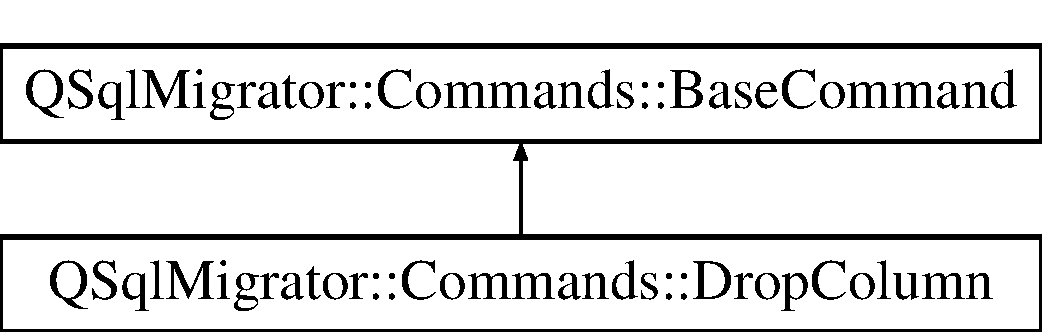
\includegraphics[height=2.000000cm]{class_q_sql_migrator_1_1_commands_1_1_drop_column}
\end{center}
\end{figure}
\subsection*{Public Member Functions}
\begin{DoxyCompactItemize}
\item 
\mbox{\Hypertarget{class_q_sql_migrator_1_1_commands_1_1_drop_column_a86446f01512daae2f643cfffcd4c3604}\label{class_q_sql_migrator_1_1_commands_1_1_drop_column_a86446f01512daae2f643cfffcd4c3604}} 
\hyperlink{class_q_sql_migrator_1_1_commands_1_1_drop_column_a86446f01512daae2f643cfffcd4c3604}{Drop\+Column} (const Q\+String \&column\+Name, const Q\+String \&table\+Name)
\begin{DoxyCompactList}\small\item\em Constructs the command to drop a column by name (but cannot restore it) \end{DoxyCompactList}\item 
\mbox{\Hypertarget{class_q_sql_migrator_1_1_commands_1_1_drop_column_abf379920350d2e15ad7917dd2d27d9e8}\label{class_q_sql_migrator_1_1_commands_1_1_drop_column_abf379920350d2e15ad7917dd2d27d9e8}} 
\hyperlink{class_q_sql_migrator_1_1_commands_1_1_drop_column_abf379920350d2e15ad7917dd2d27d9e8}{Drop\+Column} (const \hyperlink{class_q_sql_migrator_1_1_structure_1_1_column}{Structure\+::\+Column} \&column, const Q\+String \&table\+Name)
\begin{DoxyCompactList}\small\item\em Constructs the command to drop a column with a column definition, allowing a restore. \end{DoxyCompactList}\item 
\mbox{\Hypertarget{class_q_sql_migrator_1_1_commands_1_1_drop_column_af3f92bd1ca3e275f3c8cc57cf70bbc13}\label{class_q_sql_migrator_1_1_commands_1_1_drop_column_af3f92bd1ca3e275f3c8cc57cf70bbc13}} 
Q\+String {\bfseries table\+Name} () const
\item 
\mbox{\Hypertarget{class_q_sql_migrator_1_1_commands_1_1_drop_column_afd3c2ddc342a9c2480b8b5c3ca3addb2}\label{class_q_sql_migrator_1_1_commands_1_1_drop_column_afd3c2ddc342a9c2480b8b5c3ca3addb2}} 
Q\+String {\bfseries column\+Name} () const
\item 
\mbox{\Hypertarget{class_q_sql_migrator_1_1_commands_1_1_drop_column_a4642dc7bbefa309fed15a950110f962a}\label{class_q_sql_migrator_1_1_commands_1_1_drop_column_a4642dc7bbefa309fed15a950110f962a}} 
const \hyperlink{class_q_sql_migrator_1_1_structure_1_1_column}{Structure\+::\+Column} \& {\bfseries column} () const
\item 
\mbox{\Hypertarget{class_q_sql_migrator_1_1_commands_1_1_drop_column_acae37beeec7fc8fce0660de2b4ef280c}\label{class_q_sql_migrator_1_1_commands_1_1_drop_column_acae37beeec7fc8fce0660de2b4ef280c}} 
Command\+Ptr {\bfseries reverse} () const Q\+\_\+\+D\+E\+C\+L\+\_\+\+O\+V\+E\+R\+R\+I\+DE
\end{DoxyCompactItemize}
\subsection*{Static Public Member Functions}
\begin{DoxyCompactItemize}
\item 
\mbox{\Hypertarget{class_q_sql_migrator_1_1_commands_1_1_drop_column_a644ce32a7e8893fcb0013fef2c92cfe1}\label{class_q_sql_migrator_1_1_commands_1_1_drop_column_a644ce32a7e8893fcb0013fef2c92cfe1}} 
static const Q\+String \& {\bfseries type\+Name} ()
\end{DoxyCompactItemize}


\subsection{Detailed Description}
value object representing the command to drop a column 

The documentation for this class was generated from the following files\+:\begin{DoxyCompactItemize}
\item 
/home/george/\+Develop/\+Praaline\+Py/praaline-\/core/\+Q\+Sql\+Migrator/\+Commands/Drop\+Column.\+h\item 
/home/george/\+Develop/\+Praaline\+Py/praaline-\/core/\+Q\+Sql\+Migrator/\+Commands/Drop\+Column.\+cpp\end{DoxyCompactItemize}

\hypertarget{class_q_sql_migrator_1_1_commands_1_1_drop_index}{}\section{Q\+Sql\+Migrator\+:\+:Commands\+:\+:Drop\+Index Class Reference}
\label{class_q_sql_migrator_1_1_commands_1_1_drop_index}\index{Q\+Sql\+Migrator\+::\+Commands\+::\+Drop\+Index@{Q\+Sql\+Migrator\+::\+Commands\+::\+Drop\+Index}}


value object representing the command to drop an index  




{\ttfamily \#include $<$Drop\+Index.\+h$>$}

Inheritance diagram for Q\+Sql\+Migrator\+:\+:Commands\+:\+:Drop\+Index\+:\begin{figure}[H]
\begin{center}
\leavevmode
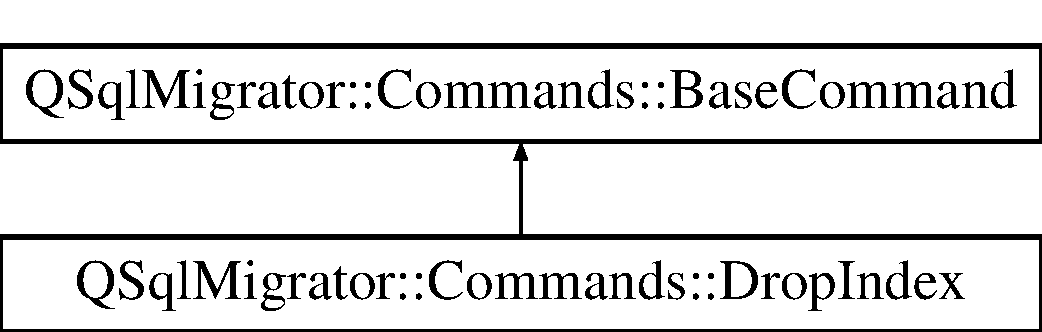
\includegraphics[height=2.000000cm]{class_q_sql_migrator_1_1_commands_1_1_drop_index}
\end{center}
\end{figure}
\subsection*{Public Member Functions}
\begin{DoxyCompactItemize}
\item 
\mbox{\Hypertarget{class_q_sql_migrator_1_1_commands_1_1_drop_index_a76c4467f46ad442751cfe80e07ef37eb}\label{class_q_sql_migrator_1_1_commands_1_1_drop_index_a76c4467f46ad442751cfe80e07ef37eb}} 
{\bfseries Drop\+Index} (const Q\+String \&name)
\item 
\mbox{\Hypertarget{class_q_sql_migrator_1_1_commands_1_1_drop_index_a916fb44757c2e8ae465b180508327cfc}\label{class_q_sql_migrator_1_1_commands_1_1_drop_index_a916fb44757c2e8ae465b180508327cfc}} 
{\bfseries Drop\+Index} (const \hyperlink{class_q_sql_migrator_1_1_structure_1_1_index}{Structure\+::\+Index} \&index)
\item 
\mbox{\Hypertarget{class_q_sql_migrator_1_1_commands_1_1_drop_index_a503215d44baf099fd8fc59e607ae8a53}\label{class_q_sql_migrator_1_1_commands_1_1_drop_index_a503215d44baf099fd8fc59e607ae8a53}} 
const \hyperlink{class_q_sql_migrator_1_1_structure_1_1_index}{Structure\+::\+Index} \& {\bfseries index} () const
\item 
\mbox{\Hypertarget{class_q_sql_migrator_1_1_commands_1_1_drop_index_aa9c9ca93e97251de0a779e4b15ce1d23}\label{class_q_sql_migrator_1_1_commands_1_1_drop_index_aa9c9ca93e97251de0a779e4b15ce1d23}} 
const Q\+String \& {\bfseries name} () const
\item 
\mbox{\Hypertarget{class_q_sql_migrator_1_1_commands_1_1_drop_index_a90fa2bbaba6ef98eafa87417d7243dfe}\label{class_q_sql_migrator_1_1_commands_1_1_drop_index_a90fa2bbaba6ef98eafa87417d7243dfe}} 
Command\+Ptr {\bfseries reverse} () const Q\+\_\+\+D\+E\+C\+L\+\_\+\+O\+V\+E\+R\+R\+I\+DE
\end{DoxyCompactItemize}
\subsection*{Static Public Member Functions}
\begin{DoxyCompactItemize}
\item 
\mbox{\Hypertarget{class_q_sql_migrator_1_1_commands_1_1_drop_index_af082e18d086ba9bfc9c914c32a1a8822}\label{class_q_sql_migrator_1_1_commands_1_1_drop_index_af082e18d086ba9bfc9c914c32a1a8822}} 
static const Q\+String \& {\bfseries type\+Name} ()
\end{DoxyCompactItemize}


\subsection{Detailed Description}
value object representing the command to drop an index 

The documentation for this class was generated from the following files\+:\begin{DoxyCompactItemize}
\item 
/home/george/\+Develop/\+Praaline\+Py/praaline-\/core/\+Q\+Sql\+Migrator/\+Commands/Drop\+Index.\+h\item 
/home/george/\+Develop/\+Praaline\+Py/praaline-\/core/\+Q\+Sql\+Migrator/\+Commands/Drop\+Index.\+cpp\end{DoxyCompactItemize}

\hypertarget{class_q_sql_migrator_1_1_commands_1_1_drop_table}{}\section{Q\+Sql\+Migrator\+:\+:Commands\+:\+:Drop\+Table Class Reference}
\label{class_q_sql_migrator_1_1_commands_1_1_drop_table}\index{Q\+Sql\+Migrator\+::\+Commands\+::\+Drop\+Table@{Q\+Sql\+Migrator\+::\+Commands\+::\+Drop\+Table}}


value object representing the command to drop a table  




{\ttfamily \#include $<$Drop\+Table.\+h$>$}

Inheritance diagram for Q\+Sql\+Migrator\+:\+:Commands\+:\+:Drop\+Table\+:\begin{figure}[H]
\begin{center}
\leavevmode
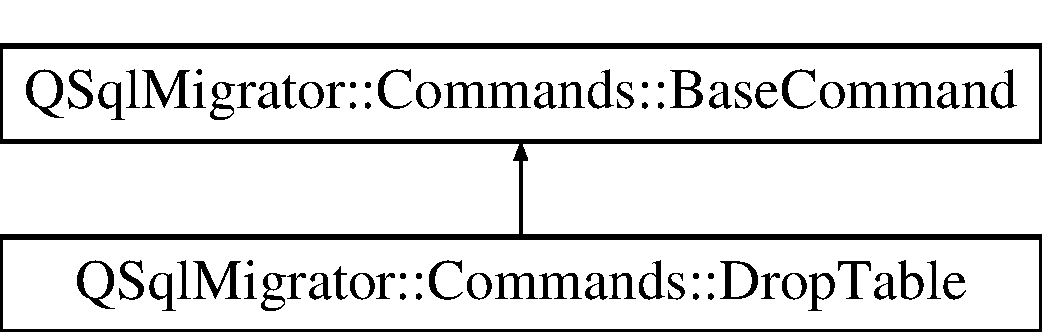
\includegraphics[height=2.000000cm]{class_q_sql_migrator_1_1_commands_1_1_drop_table}
\end{center}
\end{figure}
\subsection*{Public Member Functions}
\begin{DoxyCompactItemize}
\item 
\mbox{\Hypertarget{class_q_sql_migrator_1_1_commands_1_1_drop_table_a5614e91b2546afaa7496b7ebaa2626a0}\label{class_q_sql_migrator_1_1_commands_1_1_drop_table_a5614e91b2546afaa7496b7ebaa2626a0}} 
{\bfseries Drop\+Table} (const Q\+String \&name)
\item 
\mbox{\Hypertarget{class_q_sql_migrator_1_1_commands_1_1_drop_table_af631db3f5276b36f2a37319b580a5fe9}\label{class_q_sql_migrator_1_1_commands_1_1_drop_table_af631db3f5276b36f2a37319b580a5fe9}} 
{\bfseries Drop\+Table} (const \hyperlink{class_q_sql_migrator_1_1_structure_1_1_table}{Structure\+::\+Table} \&table)
\item 
\mbox{\Hypertarget{class_q_sql_migrator_1_1_commands_1_1_drop_table_a17d5d22d2c4246ac50ec3dd4637eca20}\label{class_q_sql_migrator_1_1_commands_1_1_drop_table_a17d5d22d2c4246ac50ec3dd4637eca20}} 
const \hyperlink{class_q_sql_migrator_1_1_structure_1_1_table}{Structure\+::\+Table} \& {\bfseries table} () const
\item 
\mbox{\Hypertarget{class_q_sql_migrator_1_1_commands_1_1_drop_table_a0c6c39b4da845853a2cf5ba9699dbc83}\label{class_q_sql_migrator_1_1_commands_1_1_drop_table_a0c6c39b4da845853a2cf5ba9699dbc83}} 
const Q\+String \& {\bfseries table\+Name} () const
\item 
\mbox{\Hypertarget{class_q_sql_migrator_1_1_commands_1_1_drop_table_a8436f051ee9d65ac9fc8d65a2b6d91ac}\label{class_q_sql_migrator_1_1_commands_1_1_drop_table_a8436f051ee9d65ac9fc8d65a2b6d91ac}} 
Command\+Ptr {\bfseries reverse} () const Q\+\_\+\+D\+E\+C\+L\+\_\+\+O\+V\+E\+R\+R\+I\+DE
\end{DoxyCompactItemize}
\subsection*{Static Public Member Functions}
\begin{DoxyCompactItemize}
\item 
\mbox{\Hypertarget{class_q_sql_migrator_1_1_commands_1_1_drop_table_aca96d6d0a49a212ffa3f79926e9c9d4c}\label{class_q_sql_migrator_1_1_commands_1_1_drop_table_aca96d6d0a49a212ffa3f79926e9c9d4c}} 
static const Q\+String \& {\bfseries type\+Name} ()
\end{DoxyCompactItemize}


\subsection{Detailed Description}
value object representing the command to drop a table 

The documentation for this class was generated from the following files\+:\begin{DoxyCompactItemize}
\item 
/home/george/\+Develop/\+Praaline\+Py/praaline-\/core/\+Q\+Sql\+Migrator/\+Commands/Drop\+Table.\+h\item 
/home/george/\+Develop/\+Praaline\+Py/praaline-\/core/\+Q\+Sql\+Migrator/\+Commands/Drop\+Table.\+cpp\end{DoxyCompactItemize}

\hypertarget{class_e_l_a_n_annotation}{}\section{E\+L\+A\+N\+Annotation Class Reference}
\label{class_e_l_a_n_annotation}\index{E\+L\+A\+N\+Annotation@{E\+L\+A\+N\+Annotation}}


The documentation for this class was generated from the following files\+:\begin{DoxyCompactItemize}
\item 
/home/george/\+Develop/\+Praaline\+Py/praaline-\/core/interfaces/elan/E\+L\+A\+N\+Annotation.\+h\item 
/home/george/\+Develop/\+Praaline\+Py/praaline-\/core/interfaces/elan/E\+L\+A\+N\+Annotation.\+cpp\end{DoxyCompactItemize}

\hypertarget{class_exmaralda_basic_transcription_1_1_event_info}{}\section{Exmaralda\+Basic\+Transcription\+:\+:Event\+Info Class Reference}
\label{class_exmaralda_basic_transcription_1_1_event_info}\index{Exmaralda\+Basic\+Transcription\+::\+Event\+Info@{Exmaralda\+Basic\+Transcription\+::\+Event\+Info}}
\subsection*{Public Attributes}
\begin{DoxyCompactItemize}
\item 
\mbox{\Hypertarget{class_exmaralda_basic_transcription_1_1_event_info_ae589a11137f4c1e617c6e3fc4dda339e}\label{class_exmaralda_basic_transcription_1_1_event_info_ae589a11137f4c1e617c6e3fc4dda339e}} 
Q\+String {\bfseries start}
\item 
\mbox{\Hypertarget{class_exmaralda_basic_transcription_1_1_event_info_a86f307afc2e024c2dc91e96da1221afc}\label{class_exmaralda_basic_transcription_1_1_event_info_a86f307afc2e024c2dc91e96da1221afc}} 
Q\+String {\bfseries end}
\item 
\mbox{\Hypertarget{class_exmaralda_basic_transcription_1_1_event_info_a7f217e4556fa89b6ff07f7788ef35002}\label{class_exmaralda_basic_transcription_1_1_event_info_a7f217e4556fa89b6ff07f7788ef35002}} 
Q\+String {\bfseries text}
\end{DoxyCompactItemize}


The documentation for this class was generated from the following file\+:\begin{DoxyCompactItemize}
\item 
/home/george/\+Develop/\+Praaline\+Py/praaline-\/core/interfaces/exmaralda/Exmaralda\+Basic\+Transcription.\+h\end{DoxyCompactItemize}

\hypertarget{class_exmaralda_basic_transcription}{}\section{Exmaralda\+Basic\+Transcription Class Reference}
\label{class_exmaralda_basic_transcription}\index{Exmaralda\+Basic\+Transcription@{Exmaralda\+Basic\+Transcription}}
Inheritance diagram for Exmaralda\+Basic\+Transcription\+:\begin{figure}[H]
\begin{center}
\leavevmode
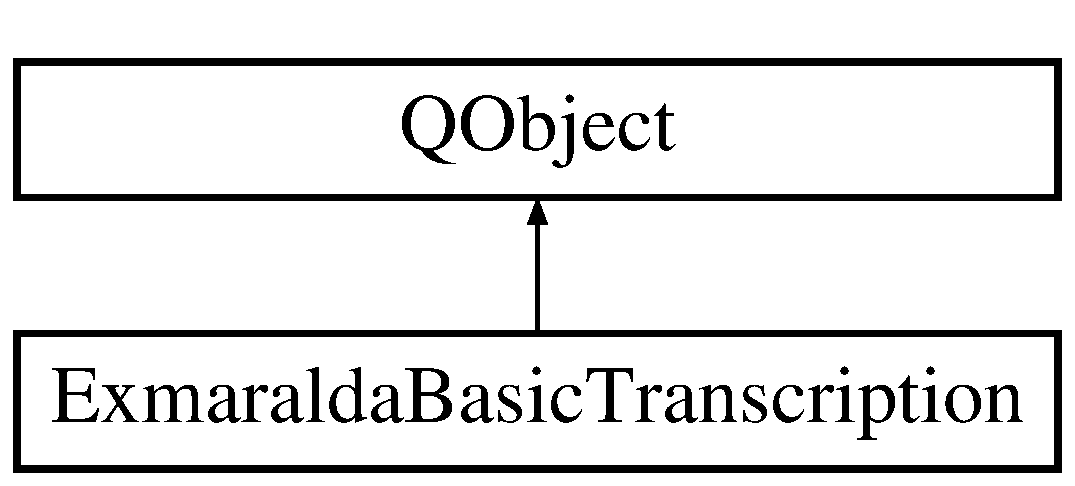
\includegraphics[height=2.000000cm]{class_exmaralda_basic_transcription}
\end{center}
\end{figure}
\subsection*{Classes}
\begin{DoxyCompactItemize}
\item 
class \hyperlink{class_exmaralda_basic_transcription_1_1_event_info}{Event\+Info}
\item 
class \hyperlink{class_exmaralda_basic_transcription_1_1_speaker_info}{Speaker\+Info}
\item 
class \hyperlink{class_exmaralda_basic_transcription_1_1_tier_info}{Tier\+Info}
\item 
class \hyperlink{class_exmaralda_basic_transcription_1_1_timeline_info}{Timeline\+Info}
\end{DoxyCompactItemize}
\subsection*{Public Member Functions}
\begin{DoxyCompactItemize}
\item 
\mbox{\Hypertarget{class_exmaralda_basic_transcription_a86c0894cea0eff62381e237e9732e74f}\label{class_exmaralda_basic_transcription_a86c0894cea0eff62381e237e9732e74f}} 
Q\+String {\bfseries project\+Name} () const
\item 
\mbox{\Hypertarget{class_exmaralda_basic_transcription_aa60a57a1ad812755e06a84b0de876b36}\label{class_exmaralda_basic_transcription_aa60a57a1ad812755e06a84b0de876b36}} 
void {\bfseries set\+Project\+Name} (const Q\+String \&projecet\+Name)
\item 
\mbox{\Hypertarget{class_exmaralda_basic_transcription_af65c4389483b4dfc84fcae0d83e6da4e}\label{class_exmaralda_basic_transcription_af65c4389483b4dfc84fcae0d83e6da4e}} 
Q\+String {\bfseries transcription\+Name} () const
\item 
\mbox{\Hypertarget{class_exmaralda_basic_transcription_a3a3f70df20b631d3e8c4591ffa38cc19}\label{class_exmaralda_basic_transcription_a3a3f70df20b631d3e8c4591ffa38cc19}} 
void {\bfseries set\+Transcription\+Name} (const Q\+String \&transcription\+Name)
\item 
\mbox{\Hypertarget{class_exmaralda_basic_transcription_aee75ddcd98f23b21a3a0684fe08240a4}\label{class_exmaralda_basic_transcription_aee75ddcd98f23b21a3a0684fe08240a4}} 
Q\+String {\bfseries transcription\+Convention} () const
\item 
\mbox{\Hypertarget{class_exmaralda_basic_transcription_a751b55371499e2fc13cabc9fbb4df34a}\label{class_exmaralda_basic_transcription_a751b55371499e2fc13cabc9fbb4df34a}} 
void {\bfseries set\+Transcription\+Convention} (const Q\+String \&transcription\+Convention)
\item 
\mbox{\Hypertarget{class_exmaralda_basic_transcription_a68df5ee1f743006e97d264ff135b1095}\label{class_exmaralda_basic_transcription_a68df5ee1f743006e97d264ff135b1095}} 
Q\+String {\bfseries comment} () const
\item 
\mbox{\Hypertarget{class_exmaralda_basic_transcription_a4329b9f04c89df2c25dc4adc55c81390}\label{class_exmaralda_basic_transcription_a4329b9f04c89df2c25dc4adc55c81390}} 
void {\bfseries set\+Comment} (const Q\+String \&comment)
\item 
\mbox{\Hypertarget{class_exmaralda_basic_transcription_a25d2cd1fec44bff0dc008ddd9fd317c1}\label{class_exmaralda_basic_transcription_a25d2cd1fec44bff0dc008ddd9fd317c1}} 
Q\+String\+List \& {\bfseries referenced\+Files} ()
\item 
\mbox{\Hypertarget{class_exmaralda_basic_transcription_a467c002a9c90df5fa54aaa3765bd6e57}\label{class_exmaralda_basic_transcription_a467c002a9c90df5fa54aaa3765bd6e57}} 
Q\+Hash$<$ Q\+String, Q\+String $>$ \& {\bfseries ud\+Meta\+Info} ()
\item 
\mbox{\Hypertarget{class_exmaralda_basic_transcription_adf5df9b5e145617423ffba3aba3e00f1}\label{class_exmaralda_basic_transcription_adf5df9b5e145617423ffba3aba3e00f1}} 
Q\+List$<$ \hyperlink{class_exmaralda_basic_transcription_1_1_speaker_info}{Speaker\+Info} $>$ \& {\bfseries speaker\+Table} ()
\item 
\mbox{\Hypertarget{class_exmaralda_basic_transcription_ae53576dad124a6e0857e5bbc78f70b4a}\label{class_exmaralda_basic_transcription_ae53576dad124a6e0857e5bbc78f70b4a}} 
Q\+List$<$ \hyperlink{class_exmaralda_basic_transcription_1_1_timeline_info}{Timeline\+Info} $>$ \& {\bfseries common\+TL} ()
\item 
\mbox{\Hypertarget{class_exmaralda_basic_transcription_a4994d4e28a6fc109d84d36b7e97da4dd}\label{class_exmaralda_basic_transcription_a4994d4e28a6fc109d84d36b7e97da4dd}} 
Q\+Hash$<$ Q\+String, \hyperlink{class_exmaralda_basic_transcription_1_1_tier_info}{Tier\+Info} $>$ \& {\bfseries tiers} ()
\end{DoxyCompactItemize}
\subsection*{Static Public Member Functions}
\begin{DoxyCompactItemize}
\item 
\mbox{\Hypertarget{class_exmaralda_basic_transcription_a36bc1e35ef4eee398b062ffc05ca54e9}\label{class_exmaralda_basic_transcription_a36bc1e35ef4eee398b062ffc05ca54e9}} 
static bool {\bfseries load} (const Q\+String \&filename, \hyperlink{class_exmaralda_basic_transcription}{Exmaralda\+Basic\+Transcription} \&transcription)
\item 
\mbox{\Hypertarget{class_exmaralda_basic_transcription_a456e04788999b47a554ba30f105e919c}\label{class_exmaralda_basic_transcription_a456e04788999b47a554ba30f105e919c}} 
static bool {\bfseries save} (const Q\+String \&filename, \hyperlink{class_exmaralda_basic_transcription}{Exmaralda\+Basic\+Transcription} \&transcription)
\end{DoxyCompactItemize}


The documentation for this class was generated from the following files\+:\begin{DoxyCompactItemize}
\item 
/home/george/\+Develop/\+Praaline\+Py/praaline-\/core/interfaces/exmaralda/Exmaralda\+Basic\+Transcription.\+h\item 
/home/george/\+Develop/\+Praaline\+Py/praaline-\/core/interfaces/exmaralda/Exmaralda\+Basic\+Transcription.\+cpp\end{DoxyCompactItemize}

\hypertarget{class_exmaralda_transcription_bridge}{}\section{Exmaralda\+Transcription\+Bridge Class Reference}
\label{class_exmaralda_transcription_bridge}\index{Exmaralda\+Transcription\+Bridge@{Exmaralda\+Transcription\+Bridge}}
Inheritance diagram for Exmaralda\+Transcription\+Bridge\+:\begin{figure}[H]
\begin{center}
\leavevmode
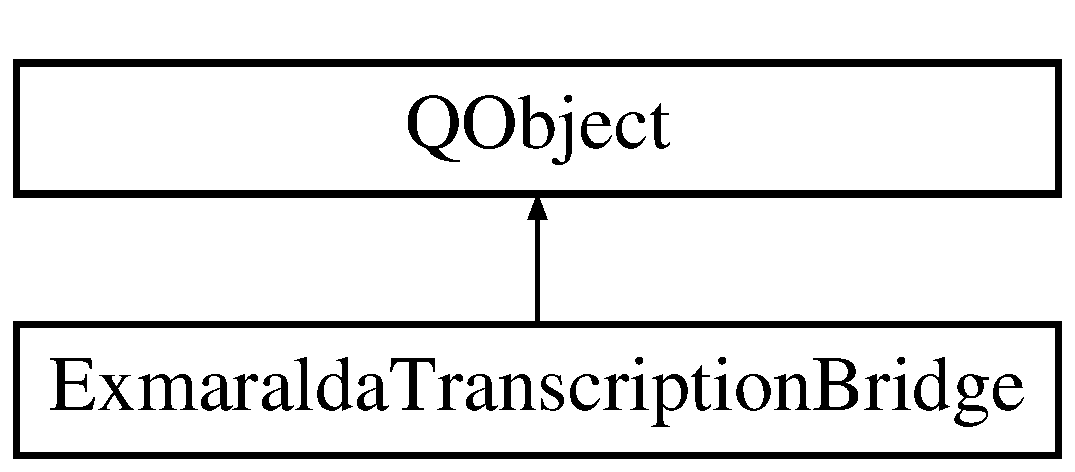
\includegraphics[height=2.000000cm]{class_exmaralda_transcription_bridge}
\end{center}
\end{figure}
\subsection*{Classes}
\begin{DoxyCompactItemize}
\item 
class \hyperlink{class_exmaralda_transcription_bridge_1_1_tier_to_export_info}{Tier\+To\+Export\+Info}
\end{DoxyCompactItemize}
\subsection*{Public Member Functions}
\begin{DoxyCompactItemize}
\item 
\mbox{\Hypertarget{class_exmaralda_transcription_bridge_a2fa2ac03488832a280321558b0c6d88d}\label{class_exmaralda_transcription_bridge_a2fa2ac03488832a280321558b0c6d88d}} 
{\bfseries Exmaralda\+Transcription\+Bridge} (Q\+Object $\ast$parent=0)
\item 
\mbox{\Hypertarget{class_exmaralda_transcription_bridge_ac19cbf007cb5d0a4fbd11c450919801a}\label{class_exmaralda_transcription_bridge_ac19cbf007cb5d0a4fbd11c450919801a}} 
void {\bfseries add\+Tier} (const Q\+String \&tier\+ID, const Q\+String \&speaker\+ID, const Q\+String \&type, const Q\+String \&category, const Q\+String \&display\+Name, \hyperlink{class_annotation_tier}{Annotation\+Tier} $\ast$tier\+To\+Export)
\item 
\mbox{\Hypertarget{class_exmaralda_transcription_bridge_a142c275e00354c7fdef8f30f9b520f3a}\label{class_exmaralda_transcription_bridge_a142c275e00354c7fdef8f30f9b520f3a}} 
void {\bfseries export\+Praaline\+To\+Partitur} (\hyperlink{class_exmaralda_basic_transcription}{Exmaralda\+Basic\+Transcription} \&partitur)
\end{DoxyCompactItemize}


The documentation for this class was generated from the following files\+:\begin{DoxyCompactItemize}
\item 
/home/george/\+Develop/\+Praaline\+Py/praaline-\/core/interfaces/exmaralda/Exmaralda\+Transcription\+Bridge.\+h\item 
/home/george/\+Develop/\+Praaline\+Py/praaline-\/core/interfaces/exmaralda/Exmaralda\+Transcription\+Bridge.\+cpp\end{DoxyCompactItemize}

\hypertarget{class_file_datastore}{}\section{File\+Datastore Class Reference}
\label{class_file_datastore}\index{File\+Datastore@{File\+Datastore}}
Inheritance diagram for File\+Datastore\+:\begin{figure}[H]
\begin{center}
\leavevmode
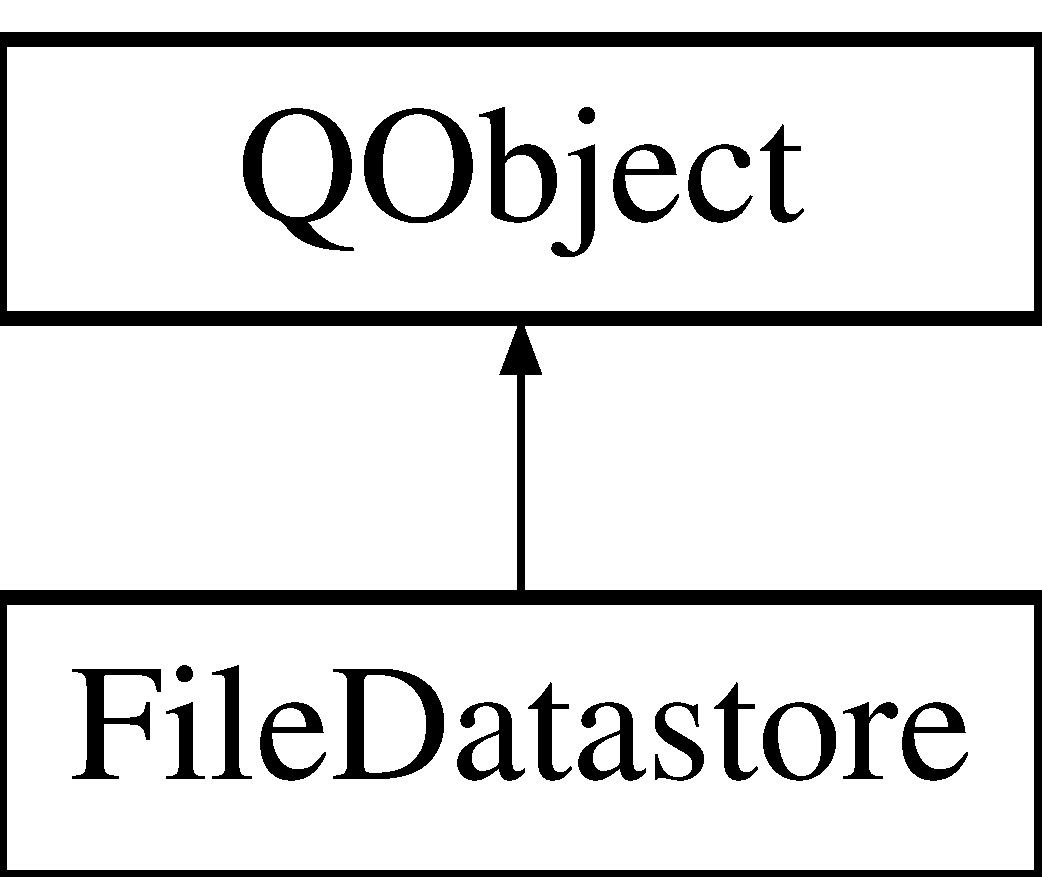
\includegraphics[height=2.000000cm]{class_file_datastore}
\end{center}
\end{figure}
\subsection*{Public Member Functions}
\begin{DoxyCompactItemize}
\item 
\mbox{\Hypertarget{class_file_datastore_a40efdf5a17f50172b477b34fd6423dda}\label{class_file_datastore_a40efdf5a17f50172b477b34fd6423dda}} 
{\bfseries File\+Datastore} (Q\+Object $\ast$parent=nullptr)
\item 
\mbox{\Hypertarget{class_file_datastore_a704f5f11d68f1778b554c32ff5525235}\label{class_file_datastore_a704f5f11d68f1778b554c32ff5525235}} 
Q\+String {\bfseries base\+Path} () const
\item 
\mbox{\Hypertarget{class_file_datastore_aa4c12673e57d0aa51c05f691051e859b}\label{class_file_datastore_aa4c12673e57d0aa51c05f691051e859b}} 
void {\bfseries set\+Base\+Path} (const Q\+String \&path)
\item 
\mbox{\Hypertarget{class_file_datastore_a9b66a3ef7f5fe951a1601f7b5b8271e4}\label{class_file_datastore_a9b66a3ef7f5fe951a1601f7b5b8271e4}} 
Q\+String {\bfseries get\+Relative\+To\+Base\+Path} (const Q\+String \&absolute\+File\+Path) const
\end{DoxyCompactItemize}
\subsection*{Protected Attributes}
\begin{DoxyCompactItemize}
\item 
\mbox{\Hypertarget{class_file_datastore_a66a2fe6eb0ed3d1417b306bb0b237e53}\label{class_file_datastore_a66a2fe6eb0ed3d1417b306bb0b237e53}} 
Q\+String {\bfseries m\+\_\+base\+Path}
\end{DoxyCompactItemize}
\subsection*{Properties}
\begin{DoxyCompactItemize}
\item 
\mbox{\Hypertarget{class_file_datastore_a7ec5358ec780ee4d8cd360741c35ea56}\label{class_file_datastore_a7ec5358ec780ee4d8cd360741c35ea56}} 
Q\+String {\bfseries base\+Path}
\end{DoxyCompactItemize}


The documentation for this class was generated from the following files\+:\begin{DoxyCompactItemize}
\item 
/home/george/\+Develop/\+Praaline\+Py/praaline-\/core/datastore/File\+Datastore.\+h\item 
/home/george/\+Develop/\+Praaline\+Py/praaline-\/core/datastore/File\+Datastore.\+cpp\end{DoxyCompactItemize}

\hypertarget{class_q_sql_migrator_1_1_helper_1_1_firebird_sql_structure_service}{}\section{Q\+Sql\+Migrator\+:\+:Helper\+:\+:Firebird\+Sql\+Structure\+Service Class Reference}
\label{class_q_sql_migrator_1_1_helper_1_1_firebird_sql_structure_service}\index{Q\+Sql\+Migrator\+::\+Helper\+::\+Firebird\+Sql\+Structure\+Service@{Q\+Sql\+Migrator\+::\+Helper\+::\+Firebird\+Sql\+Structure\+Service}}
Inheritance diagram for Q\+Sql\+Migrator\+:\+:Helper\+:\+:Firebird\+Sql\+Structure\+Service\+:\begin{figure}[H]
\begin{center}
\leavevmode
\includegraphics[height=2.000000cm]{class_q_sql_migrator_1_1_helper_1_1_firebird_sql_structure_service}
\end{center}
\end{figure}
\subsection*{Public Member Functions}
\begin{DoxyCompactItemize}
\item 
\hyperlink{class_q_sql_migrator_1_1_structure_1_1_table}{Structure\+::\+Table} \hyperlink{class_q_sql_migrator_1_1_helper_1_1_firebird_sql_structure_service_aface10de417ab9e0e749cfe2f53728e6}{get\+Table\+Definition} (const Q\+String \&table\+Name, Q\+Sql\+Database database) const Q\+\_\+\+D\+E\+C\+L\+\_\+\+O\+V\+E\+R\+R\+I\+DE
\item 
\hyperlink{class_q_sql_migrator_1_1_structure_1_1_index}{Structure\+::\+Index} \hyperlink{class_q_sql_migrator_1_1_helper_1_1_firebird_sql_structure_service_ae11053be8caa809aae7724741dc68c2b}{get\+Index\+Definition} (const Q\+String \&index\+Name, const Q\+String \&table\+Name, Q\+Sql\+Database database) const Q\+\_\+\+D\+E\+C\+L\+\_\+\+O\+V\+E\+R\+R\+I\+DE
\end{DoxyCompactItemize}


\subsection{Member Function Documentation}
\mbox{\Hypertarget{class_q_sql_migrator_1_1_helper_1_1_firebird_sql_structure_service_ae11053be8caa809aae7724741dc68c2b}\label{class_q_sql_migrator_1_1_helper_1_1_firebird_sql_structure_service_ae11053be8caa809aae7724741dc68c2b}} 
\index{Q\+Sql\+Migrator\+::\+Helper\+::\+Firebird\+Sql\+Structure\+Service@{Q\+Sql\+Migrator\+::\+Helper\+::\+Firebird\+Sql\+Structure\+Service}!get\+Index\+Definition@{get\+Index\+Definition}}
\index{get\+Index\+Definition@{get\+Index\+Definition}!Q\+Sql\+Migrator\+::\+Helper\+::\+Firebird\+Sql\+Structure\+Service@{Q\+Sql\+Migrator\+::\+Helper\+::\+Firebird\+Sql\+Structure\+Service}}
\subsubsection{\texorpdfstring{get\+Index\+Definition()}{getIndexDefinition()}}
{\footnotesize\ttfamily \hyperlink{class_q_sql_migrator_1_1_structure_1_1_index}{Structure\+::\+Index} Q\+Sql\+Migrator\+::\+Helper\+::\+Firebird\+Sql\+Structure\+Service\+::get\+Index\+Definition (\begin{DoxyParamCaption}\item[{const Q\+String \&}]{index\+Name,  }\item[{const Q\+String \&}]{table\+Name,  }\item[{Q\+Sql\+Database}]{database }\end{DoxyParamCaption}) const\hspace{0.3cm}{\ttfamily [virtual]}}

\begin{DoxyReturn}{Returns}
the definition of an existing index in the database for a table 
\end{DoxyReturn}


Implements \hyperlink{class_q_sql_migrator_1_1_helper_1_1_sql_structure_service_ab62049f95710fc0965097f08b410e790}{Q\+Sql\+Migrator\+::\+Helper\+::\+Sql\+Structure\+Service}.

\mbox{\Hypertarget{class_q_sql_migrator_1_1_helper_1_1_firebird_sql_structure_service_aface10de417ab9e0e749cfe2f53728e6}\label{class_q_sql_migrator_1_1_helper_1_1_firebird_sql_structure_service_aface10de417ab9e0e749cfe2f53728e6}} 
\index{Q\+Sql\+Migrator\+::\+Helper\+::\+Firebird\+Sql\+Structure\+Service@{Q\+Sql\+Migrator\+::\+Helper\+::\+Firebird\+Sql\+Structure\+Service}!get\+Table\+Definition@{get\+Table\+Definition}}
\index{get\+Table\+Definition@{get\+Table\+Definition}!Q\+Sql\+Migrator\+::\+Helper\+::\+Firebird\+Sql\+Structure\+Service@{Q\+Sql\+Migrator\+::\+Helper\+::\+Firebird\+Sql\+Structure\+Service}}
\subsubsection{\texorpdfstring{get\+Table\+Definition()}{getTableDefinition()}}
{\footnotesize\ttfamily \hyperlink{class_q_sql_migrator_1_1_structure_1_1_table}{Table} Q\+Sql\+Migrator\+::\+Helper\+::\+Firebird\+Sql\+Structure\+Service\+::get\+Table\+Definition (\begin{DoxyParamCaption}\item[{const Q\+String \&}]{table\+Name,  }\item[{Q\+Sql\+Database}]{database }\end{DoxyParamCaption}) const\hspace{0.3cm}{\ttfamily [virtual]}}

\begin{DoxyReturn}{Returns}
the definition of an existing table in the databse 
\end{DoxyReturn}


Implements \hyperlink{class_q_sql_migrator_1_1_helper_1_1_sql_structure_service_abb2f11402700c1a1e52d596431255e8a}{Q\+Sql\+Migrator\+::\+Helper\+::\+Sql\+Structure\+Service}.



The documentation for this class was generated from the following files\+:\begin{DoxyCompactItemize}
\item 
/home/george/\+Develop/\+Praaline\+Py/praaline-\/core/\+Q\+Sql\+Migrator/\+Databases/\+Firebird\+Migrator/\+Helper/Firebird\+Sql\+Structure\+Service.\+h\item 
/home/george/\+Develop/\+Praaline\+Py/praaline-\/core/\+Q\+Sql\+Migrator/\+Databases/\+Firebird\+Migrator/\+Helper/Firebird\+Sql\+Structure\+Service.\+cpp\end{DoxyCompactItemize}

\hypertarget{class_q_sql_migrator_1_1_helper_1_1_helper_repository}{}\section{Q\+Sql\+Migrator\+:\+:Helper\+:\+:Helper\+Repository Class Reference}
\label{class_q_sql_migrator_1_1_helper_1_1_helper_repository}\index{Q\+Sql\+Migrator\+::\+Helper\+::\+Helper\+Repository@{Q\+Sql\+Migrator\+::\+Helper\+::\+Helper\+Repository}}


a simple repository of all helper classes  




{\ttfamily \#include $<$Helper\+Repository.\+h$>$}

\subsection*{Public Member Functions}
\begin{DoxyCompactItemize}
\item 
\mbox{\Hypertarget{class_q_sql_migrator_1_1_helper_1_1_helper_repository_a792d551f34b97a943b9dd0684dfa40cd}\label{class_q_sql_migrator_1_1_helper_1_1_helper_repository_a792d551f34b97a943b9dd0684dfa40cd}} 
{\bfseries Helper\+Repository} (const \hyperlink{class_q_sql_migrator_1_1_helper_1_1_quote_service}{Quote\+Service} \&quote\+Service, const \hyperlink{class_q_sql_migrator_1_1_helper_1_1_type_mapper_service}{Type\+Mapper\+Service} \&type\+Mapper\+Service, const \hyperlink{class_q_sql_migrator_1_1_helper_1_1_column_service}{Column\+Service} \&column\+Service, const \hyperlink{class_q_sql_migrator_1_1_helper_1_1_sql_structure_service}{Sql\+Structure\+Service} \&sql\+Structure\+Service)
\item 
\mbox{\Hypertarget{class_q_sql_migrator_1_1_helper_1_1_helper_repository_a1c2e73191c625c5f7d2a0d9eebce9c89}\label{class_q_sql_migrator_1_1_helper_1_1_helper_repository_a1c2e73191c625c5f7d2a0d9eebce9c89}} 
const \hyperlink{class_q_sql_migrator_1_1_helper_1_1_quote_service}{Quote\+Service} \& {\bfseries quote\+Service} () const
\item 
\mbox{\Hypertarget{class_q_sql_migrator_1_1_helper_1_1_helper_repository_a149d37f18d261c626f29b7f406de304b}\label{class_q_sql_migrator_1_1_helper_1_1_helper_repository_a149d37f18d261c626f29b7f406de304b}} 
const \hyperlink{class_q_sql_migrator_1_1_helper_1_1_type_mapper_service}{Type\+Mapper\+Service} \& {\bfseries type\+Mapper\+Service} () const
\item 
\mbox{\Hypertarget{class_q_sql_migrator_1_1_helper_1_1_helper_repository_ad24723b30bad0169b63277363536897f}\label{class_q_sql_migrator_1_1_helper_1_1_helper_repository_ad24723b30bad0169b63277363536897f}} 
const \hyperlink{class_q_sql_migrator_1_1_helper_1_1_column_service}{Column\+Service} \& {\bfseries column\+Service} () const
\item 
\mbox{\Hypertarget{class_q_sql_migrator_1_1_helper_1_1_helper_repository_a8a2b7b477bce1d022e433f1af95a8660}\label{class_q_sql_migrator_1_1_helper_1_1_helper_repository_a8a2b7b477bce1d022e433f1af95a8660}} 
const \hyperlink{class_q_sql_migrator_1_1_helper_1_1_sql_structure_service}{Sql\+Structure\+Service} \& {\bfseries sql\+Structure\+Service} () const
\end{DoxyCompactItemize}


\subsection{Detailed Description}
a simple repository of all helper classes 

The documentation for this class was generated from the following files\+:\begin{DoxyCompactItemize}
\item 
/home/george/\+Develop/\+Praaline\+Py/praaline-\/core/\+Q\+Sql\+Migrator/\+Helper/Helper\+Repository.\+h\item 
/home/george/\+Develop/\+Praaline\+Py/praaline-\/core/\+Q\+Sql\+Migrator/\+Helper/Helper\+Repository.\+cpp\end{DoxyCompactItemize}

\hypertarget{class_histogram_calculator}{}\section{Histogram\+Calculator Class Reference}
\label{class_histogram_calculator}\index{Histogram\+Calculator@{Histogram\+Calculator}}
\subsection*{Public Member Functions}
\begin{DoxyCompactItemize}
\item 
\mbox{\Hypertarget{class_histogram_calculator_afbaca8c20aac86708acb2cc97d4c22bd}\label{class_histogram_calculator_afbaca8c20aac86708acb2cc97d4c22bd}} 
void {\bfseries set\+Values} (const Q\+List$<$ double $>$ \&values)
\item 
\mbox{\Hypertarget{class_histogram_calculator_a8eb9e4db27d7d14b0f621c5870e7ccdc}\label{class_histogram_calculator_a8eb9e4db27d7d14b0f621c5870e7ccdc}} 
void {\bfseries set\+Minimum} (double min)
\item 
\mbox{\Hypertarget{class_histogram_calculator_acf58b8167de843f628ec3756bafbd766}\label{class_histogram_calculator_acf58b8167de843f628ec3756bafbd766}} 
void {\bfseries set\+Maximum} (double max)
\item 
\mbox{\Hypertarget{class_histogram_calculator_a72bdc4fe645a7197ede79a88eabaf37d}\label{class_histogram_calculator_a72bdc4fe645a7197ede79a88eabaf37d}} 
double {\bfseries optimal\+Bin\+Width} () const
\item 
\mbox{\Hypertarget{class_histogram_calculator_ad9f572826bc52b1bf1fa87a4f8e5c151}\label{class_histogram_calculator_ad9f572826bc52b1bf1fa87a4f8e5c151}} 
int {\bfseries optimal\+Number\+Bins} () const
\item 
\mbox{\Hypertarget{class_histogram_calculator_a6129b8e0eb63b2c359e0666929d76304}\label{class_histogram_calculator_a6129b8e0eb63b2c359e0666929d76304}} 
Q\+List$<$ double $>$ {\bfseries bin\+Edges} (int bins) const
\item 
\mbox{\Hypertarget{class_histogram_calculator_ab28d0a0f98b19262eb18f595a142d854}\label{class_histogram_calculator_ab28d0a0f98b19262eb18f595a142d854}} 
Q\+List$<$ int $>$ {\bfseries counts} (int bins) const
\end{DoxyCompactItemize}


The documentation for this class was generated from the following files\+:\begin{DoxyCompactItemize}
\item 
/home/george/\+Develop/\+Praaline\+Py/praaline-\/core/statistics/Histogram\+Calculator.\+h\item 
/home/george/\+Develop/\+Praaline\+Py/praaline-\/core/statistics/Histogram\+Calculator.\+cpp\end{DoxyCompactItemize}

\hypertarget{class_i_datastore}{}\section{I\+Datastore Class Reference}
\label{class_i_datastore}\index{I\+Datastore@{I\+Datastore}}
Inheritance diagram for I\+Datastore\+:\begin{figure}[H]
\begin{center}
\leavevmode
\includegraphics[height=1.490683cm]{class_i_datastore}
\end{center}
\end{figure}
\subsection*{Static Protected Member Functions}
\begin{DoxyCompactItemize}
\item 
\mbox{\Hypertarget{class_i_datastore_a32e75a751d810a5330ae8c3ec4dbd09c}\label{class_i_datastore_a32e75a751d810a5330ae8c3ec4dbd09c}} 
static void {\bfseries set\+New} (\hyperlink{class_i_saveable}{I\+Saveable} $\ast$item)
\item 
\mbox{\Hypertarget{class_i_datastore_af97d7e04ec4844f287e903f640716e6f}\label{class_i_datastore_af97d7e04ec4844f287e903f640716e6f}} 
static void {\bfseries set\+Dirty} (\hyperlink{class_i_saveable}{I\+Saveable} $\ast$item)
\item 
\mbox{\Hypertarget{class_i_datastore_a520f8a87495a0c7486100a5cbc792b4c}\label{class_i_datastore_a520f8a87495a0c7486100a5cbc792b4c}} 
static void {\bfseries set\+Clean} (\hyperlink{class_i_saveable}{I\+Saveable} $\ast$item)
\end{DoxyCompactItemize}


The documentation for this class was generated from the following files\+:\begin{DoxyCompactItemize}
\item 
/home/george/\+Develop/\+Praaline\+Py/praaline-\/core/base/I\+Datastore.\+h\item 
/home/george/\+Develop/\+Praaline\+Py/praaline-\/core/base/I\+Datastore.\+cpp\end{DoxyCompactItemize}

\hypertarget{class_import_annotations}{}\section{Import\+Annotations Class Reference}
\label{class_import_annotations}\index{Import\+Annotations@{Import\+Annotations}}
\subsection*{Public Types}
\begin{DoxyCompactItemize}
\item 
\mbox{\Hypertarget{class_import_annotations_a676fb9042a842ff80397fd65a81163f3}\label{class_import_annotations_a676fb9042a842ff80397fd65a81163f3}} 
enum {\bfseries Speaker\+Policy} \{ {\bfseries Speaker\+Policy\+Single}, 
{\bfseries Speaker\+Policy\+Tier\+Names}, 
{\bfseries Speaker\+Policy\+Intervals}, 
{\bfseries Speaker\+Policy\+Primary\+And\+Secondary}
 \}
\end{DoxyCompactItemize}
\subsection*{Static Public Member Functions}
\begin{DoxyCompactItemize}
\item 
\mbox{\Hypertarget{class_import_annotations_af68d1f0f77fbef9061e735bd29038e77}\label{class_import_annotations_af68d1f0f77fbef9061e735bd29038e77}} 
static Speaker\+Policy {\bfseries speaker\+Policy\+From\+Int} (int i)
\item 
\mbox{\Hypertarget{class_import_annotations_aacdd4663e821715f82a730eaaccbe8b9}\label{class_import_annotations_aacdd4663e821715f82a730eaaccbe8b9}} 
static bool {\bfseries import\+Basic} (\hyperlink{class_corpus}{Corpus} $\ast$corpus, \hyperlink{class_corpus_communication}{Corpus\+Communication} $\ast$com, \hyperlink{class_corpus_annotation}{Corpus\+Annotation} $\ast$annot, Speaker\+Policy speaker\+Policy, Q\+String speaker\+ID, \hyperlink{class_annotation_tier_group}{Annotation\+Tier\+Group} $\ast$input\+Tiers, Q\+List$<$ \hyperlink{class_tier_correspondance}{Tier\+Correspondance} $>$ \&correspondances)
\end{DoxyCompactItemize}


The documentation for this class was generated from the following files\+:\begin{DoxyCompactItemize}
\item 
/home/george/\+Develop/\+Praaline\+Py/praaline-\/core/interfaces/Import\+Annotations.\+h\item 
/home/george/\+Develop/\+Praaline\+Py/praaline-\/core/interfaces/Import\+Annotations.\+cpp\end{DoxyCompactItemize}

\hypertarget{class_q_sql_migrator_1_1_structure_1_1_index}{}\section{Q\+Sql\+Migrator\+:\+:Structure\+:\+:Index Class Reference}
\label{class_q_sql_migrator_1_1_structure_1_1_index}\index{Q\+Sql\+Migrator\+::\+Structure\+::\+Index@{Q\+Sql\+Migrator\+::\+Structure\+::\+Index}}


value object representing the structure of an sql index.  




{\ttfamily \#include $<$Index.\+h$>$}

Inheritance diagram for Q\+Sql\+Migrator\+:\+:Structure\+:\+:Index\+:\begin{figure}[H]
\begin{center}
\leavevmode
\includegraphics[height=2.000000cm]{class_q_sql_migrator_1_1_structure_1_1_index}
\end{center}
\end{figure}
\subsection*{Classes}
\begin{DoxyCompactItemize}
\item 
class \hyperlink{class_q_sql_migrator_1_1_structure_1_1_index_1_1_builder}{Builder}
\begin{DoxyCompactList}\small\item\em helper to build \hyperlink{class_q_sql_migrator_1_1_structure_1_1_index}{Index} classes \end{DoxyCompactList}\item 
class \hyperlink{class_q_sql_migrator_1_1_structure_1_1_index_1_1_column}{Column}
\begin{DoxyCompactList}\small\item\em index column reference \end{DoxyCompactList}\end{DoxyCompactItemize}
\subsection*{Public Types}
\begin{DoxyCompactItemize}
\item 
\mbox{\Hypertarget{class_q_sql_migrator_1_1_structure_1_1_index_a237ef125893ca00672374a7fb3cff687}\label{class_q_sql_migrator_1_1_structure_1_1_index_a237ef125893ca00672374a7fb3cff687}} 
enum \hyperlink{class_q_sql_migrator_1_1_structure_1_1_index_a237ef125893ca00672374a7fb3cff687}{Sort\+Order} \{ {\bfseries Default} = 0, 
{\bfseries Ascending} = 0, 
{\bfseries Descending} = 1
 \}\begin{DoxyCompactList}\small\item\em index sorting order \end{DoxyCompactList}
\item 
\mbox{\Hypertarget{class_q_sql_migrator_1_1_structure_1_1_index_ac59382bc63333d2b40bfeb2bb072478b}\label{class_q_sql_migrator_1_1_structure_1_1_index_ac59382bc63333d2b40bfeb2bb072478b}} 
typedef Q\+List$<$ \hyperlink{class_q_sql_migrator_1_1_structure_1_1_index_1_1_column}{Column} $>$ {\bfseries Column\+List}
\end{DoxyCompactItemize}
\subsection*{Public Member Functions}
\begin{DoxyCompactItemize}
\item 
\mbox{\Hypertarget{class_q_sql_migrator_1_1_structure_1_1_index_a2d1e61abc66626d3a400a927b1cfa8c8}\label{class_q_sql_migrator_1_1_structure_1_1_index_a2d1e61abc66626d3a400a927b1cfa8c8}} 
{\bfseries Index} (const Q\+String \&name, const Q\+String \&table\+Name, const Column\+List \&columns)
\item 
\mbox{\Hypertarget{class_q_sql_migrator_1_1_structure_1_1_index_a5af05609bc675d9a505605b4f087d59b}\label{class_q_sql_migrator_1_1_structure_1_1_index_a5af05609bc675d9a505605b4f087d59b}} 
{\bfseries Index} (const Q\+String \&name, const Column\+List \&columns)
\item 
\mbox{\Hypertarget{class_q_sql_migrator_1_1_structure_1_1_index_a8ca6ee617199a08408036a146231e01b}\label{class_q_sql_migrator_1_1_structure_1_1_index_a8ca6ee617199a08408036a146231e01b}} 
const Q\+String \& {\bfseries name} () const
\item 
\mbox{\Hypertarget{class_q_sql_migrator_1_1_structure_1_1_index_a6bb6792e5cdb715f2dfd5280868d8544}\label{class_q_sql_migrator_1_1_structure_1_1_index_a6bb6792e5cdb715f2dfd5280868d8544}} 
const Q\+String \& {\bfseries table\+Name} () const
\item 
\mbox{\Hypertarget{class_q_sql_migrator_1_1_structure_1_1_index_aaf0d3dd89cfd92d87970b80611c16797}\label{class_q_sql_migrator_1_1_structure_1_1_index_aaf0d3dd89cfd92d87970b80611c16797}} 
const Column\+List \& {\bfseries columns} () const
\item 
\mbox{\Hypertarget{class_q_sql_migrator_1_1_structure_1_1_index_af8faac85c9b7b1838da51c2585726ff2}\label{class_q_sql_migrator_1_1_structure_1_1_index_af8faac85c9b7b1838da51c2585726ff2}} 
bool {\bfseries is\+Valid} () const
\end{DoxyCompactItemize}


\subsection{Detailed Description}
value object representing the structure of an sql index. 

The documentation for this class was generated from the following files\+:\begin{DoxyCompactItemize}
\item 
/home/george/\+Develop/\+Praaline\+Py/praaline-\/core/\+Q\+Sql\+Migrator/\+Structure/Index.\+h\item 
/home/george/\+Develop/\+Praaline\+Py/praaline-\/core/\+Q\+Sql\+Migrator/\+Structure/Index.\+cpp\end{DoxyCompactItemize}

\hypertarget{class_q_sql_migrator_1_1_structure_1_1_local_scheme_1_1_index}{}\section{Q\+Sql\+Migrator\+:\+:Structure\+:\+:Local\+Scheme\+:\+:Index Class Reference}
\label{class_q_sql_migrator_1_1_structure_1_1_local_scheme_1_1_index}\index{Q\+Sql\+Migrator\+::\+Structure\+::\+Local\+Scheme\+::\+Index@{Q\+Sql\+Migrator\+::\+Structure\+::\+Local\+Scheme\+::\+Index}}


internal Assignable version of \hyperlink{class_q_sql_migrator_1_1_structure_1_1_local_scheme_1_1_index}{Index}  




{\ttfamily \#include $<$Local\+Scheme.\+h$>$}

Inheritance diagram for Q\+Sql\+Migrator\+:\+:Structure\+:\+:Local\+Scheme\+:\+:Index\+:\begin{figure}[H]
\begin{center}
\leavevmode
\includegraphics[height=2.000000cm]{class_q_sql_migrator_1_1_structure_1_1_local_scheme_1_1_index}
\end{center}
\end{figure}
\subsection*{Public Member Functions}
\begin{DoxyCompactItemize}
\item 
\mbox{\Hypertarget{class_q_sql_migrator_1_1_structure_1_1_local_scheme_1_1_index_a213ba698de45cac71bf542e74fec4dd4}\label{class_q_sql_migrator_1_1_structure_1_1_local_scheme_1_1_index_a213ba698de45cac71bf542e74fec4dd4}} 
{\bfseries Index} (const \hyperlink{class_q_sql_migrator_1_1_structure_1_1_local_scheme_1_1_index}{Index} \&other)
\item 
\mbox{\Hypertarget{class_q_sql_migrator_1_1_structure_1_1_local_scheme_1_1_index_a8c333c7302935a906f3a99d556e6778b}\label{class_q_sql_migrator_1_1_structure_1_1_local_scheme_1_1_index_a8c333c7302935a906f3a99d556e6778b}} 
{\bfseries Index} (const \hyperlink{class_q_sql_migrator_1_1_structure_1_1_index}{Structure\+::\+Index} \&other)
\item 
\mbox{\Hypertarget{class_q_sql_migrator_1_1_structure_1_1_local_scheme_1_1_index_a77d103ab51fff050ee87a9bb1cf1857e}\label{class_q_sql_migrator_1_1_structure_1_1_local_scheme_1_1_index_a77d103ab51fff050ee87a9bb1cf1857e}} 
\hyperlink{class_q_sql_migrator_1_1_structure_1_1_local_scheme_1_1_index}{Index} \& {\bfseries operator=} (const \hyperlink{class_q_sql_migrator_1_1_structure_1_1_local_scheme_1_1_index}{Index} \&other)
\end{DoxyCompactItemize}
\subsection*{Additional Inherited Members}


\subsection{Detailed Description}
internal Assignable version of \hyperlink{class_q_sql_migrator_1_1_structure_1_1_local_scheme_1_1_index}{Index} 

The documentation for this class was generated from the following files\+:\begin{DoxyCompactItemize}
\item 
/home/george/\+Develop/\+Praaline\+Py/praaline-\/core/\+Q\+Sql\+Migrator/\+Structure/Local\+Scheme.\+h\item 
/home/george/\+Develop/\+Praaline\+Py/praaline-\/core/\+Q\+Sql\+Migrator/\+Structure/Local\+Scheme.\+cpp\end{DoxyCompactItemize}

\hypertarget{class_interface_text_file}{}\section{Interface\+Text\+File Class Reference}
\label{class_interface_text_file}\index{Interface\+Text\+File@{Interface\+Text\+File}}
Inheritance diagram for Interface\+Text\+File\+:\begin{figure}[H]
\begin{center}
\leavevmode
\includegraphics[height=1.856354cm]{class_interface_text_file}
\end{center}
\end{figure}
\subsection*{Static Public Member Functions}
\begin{DoxyCompactItemize}
\item 
\mbox{\Hypertarget{class_interface_text_file_aae72c50b770e9a39d76191e2c57de6c7}\label{class_interface_text_file_aae72c50b770e9a39d76191e2c57de6c7}} 
static void {\bfseries set\+Default\+Encoding} (const Q\+String \&encoding)
\item 
\mbox{\Hypertarget{class_interface_text_file_a0350b78708ea6e1edb4ed9b95d18b18c}\label{class_interface_text_file_a0350b78708ea6e1edb4ed9b95d18b18c}} 
static Q\+String {\bfseries default\+Encoding} ()
\end{DoxyCompactItemize}
\subsection*{Static Protected Member Functions}
\begin{DoxyCompactItemize}
\item 
\mbox{\Hypertarget{class_interface_text_file_a4535a47b064c244f5fc652a6e8506707}\label{class_interface_text_file_a4535a47b064c244f5fc652a6e8506707}} 
static void {\bfseries detect\+Encoding} (Q\+File \&file, Q\+Text\+Stream \&stream)
\end{DoxyCompactItemize}
\subsection*{Static Protected Attributes}
\begin{DoxyCompactItemize}
\item 
\mbox{\Hypertarget{class_interface_text_file_a9255f267c6c53aa5ac1b02bffbb23b10}\label{class_interface_text_file_a9255f267c6c53aa5ac1b02bffbb23b10}} 
static Q\+String {\bfseries m\+\_\+default\+Encoding} = \char`\"{}I\+SO 8859-\/1\char`\"{}
\end{DoxyCompactItemize}


The documentation for this class was generated from the following files\+:\begin{DoxyCompactItemize}
\item 
/home/george/\+Develop/\+Praaline\+Py/praaline-\/core/interfaces/Interface\+Text\+File.\+h\item 
/home/george/\+Develop/\+Praaline\+Py/praaline-\/core/interfaces/Interface\+Text\+File.\+cpp\end{DoxyCompactItemize}

\hypertarget{class_interval}{}\section{Interval Class Reference}
\label{class_interval}\index{Interval@{Interval}}


The \hyperlink{class_interval}{Interval} class represents an annotation element that spans an interval on the timeline, i.\+e. has a start time and an end time, as well as a label and attributes. An \hyperlink{class_interval_tier}{Interval\+Tier} contains Intervals.  




{\ttfamily \#include $<$Interval.\+h$>$}

Inheritance diagram for Interval\+:\begin{figure}[H]
\begin{center}
\leavevmode
\includegraphics[height=3.000000cm]{class_interval}
\end{center}
\end{figure}
\subsection*{Public Member Functions}
\begin{DoxyCompactItemize}
\item 
\mbox{\Hypertarget{class_interval_a115ec019acb96b75bd872cbb871f54e5}\label{class_interval_a115ec019acb96b75bd872cbb871f54e5}} 
\hyperlink{class_interval_a115ec019acb96b75bd872cbb871f54e5}{Interval} ()
\begin{DoxyCompactList}\small\item\em Default constructor. \end{DoxyCompactList}\item 
\hyperlink{class_interval_a2a823516ca46649463bb83f046093ba1}{Interval} (const \hyperlink{struct_real_time}{Real\+Time} \hyperlink{class_interval_aba4daaa96ab1085b72cf19c896401593}{t\+Min}, const \hyperlink{struct_real_time}{Real\+Time} \hyperlink{class_interval_ab9efa1b25d5e4997d99ad0f360c7b2d7}{t\+Max}, const Q\+String \&\hyperlink{class_annotation_element_aa59bd98501e3882990681f6aff2ee863}{text}=Q\+String(), const Q\+Hash$<$ Q\+String, Q\+Variant $>$ \&\hyperlink{class_annotation_element_a58082d92f50c4fde2d18ce24ef3fd283}{attributes}=Q\+Hash$<$ Q\+String, Q\+Variant $>$())
\begin{DoxyCompactList}\small\item\em Constructor. \end{DoxyCompactList}\item 
\hyperlink{class_interval_a41ac30b52ead595e870fde9c8c18e0e3}{Interval} (const \hyperlink{class_interval}{Interval} \&copy)
\begin{DoxyCompactList}\small\item\em Copy constructor. \end{DoxyCompactList}\item 
\mbox{\Hypertarget{class_interval_addc606ef4606aaee647b3b68086017fa}\label{class_interval_addc606ef4606aaee647b3b68086017fa}} 
virtual \hyperlink{class_interval_addc606ef4606aaee647b3b68086017fa}{$\sim$\+Interval} () override
\begin{DoxyCompactList}\small\item\em Destructor (virtual). \end{DoxyCompactList}\item 
\hyperlink{struct_real_time}{Real\+Time} \hyperlink{class_interval_aba4daaa96ab1085b72cf19c896401593}{t\+Min} () const
\begin{DoxyCompactList}\small\item\em t\+Min property \end{DoxyCompactList}\item 
\hyperlink{struct_real_time}{Real\+Time} \hyperlink{class_interval_ab9efa1b25d5e4997d99ad0f360c7b2d7}{t\+Max} () const
\begin{DoxyCompactList}\small\item\em t\+Max property \end{DoxyCompactList}\item 
\hyperlink{struct_real_time}{Real\+Time} \hyperlink{class_interval_aa2f9a9cd972d33c1eb3af5e760e759b0}{t\+Center} () const
\begin{DoxyCompactList}\small\item\em t\+Center property \end{DoxyCompactList}\item 
\hyperlink{struct_real_time}{Real\+Time} \hyperlink{class_interval_a1b35d8374a045798f2cdc19d365855de}{duration} () const
\begin{DoxyCompactList}\small\item\em duration property \end{DoxyCompactList}\item 
virtual Q\+Variant \hyperlink{class_interval_aebcaee36c1adf49669d8a0faa16a335f}{attribute} (const Q\+String \&name) const override
\begin{DoxyCompactList}\small\item\em attribute \end{DoxyCompactList}\item 
virtual void \hyperlink{class_interval_a0895204effc21e1f4ead9b78b4b9726f}{set\+Attribute} (const Q\+String \&name, Q\+Variant value) override
\begin{DoxyCompactList}\small\item\em set\+Attribute \end{DoxyCompactList}\item 
virtual \hyperlink{class_annotation_element_af5282990ffbe25eeea8ab02037e344b0}{Element\+Type} \hyperlink{class_interval_a3ea5342504df09262d59cd2ab1658804}{element\+Type} () const override
\begin{DoxyCompactList}\small\item\em element\+Type \end{DoxyCompactList}\item 
\mbox{\Hypertarget{class_interval_a06203012d1dd561adb205db6d578e433}\label{class_interval_a06203012d1dd561adb205db6d578e433}} 
bool {\bfseries overlaps} (const \hyperlink{class_interval}{Interval} \&other, const \hyperlink{struct_real_time}{Real\+Time} threshold=\hyperlink{struct_real_time}{Real\+Time}(0, 0)) const
\item 
\mbox{\Hypertarget{class_interval_a5f7771aff890c149e17a3d42e64cf28f}\label{class_interval_a5f7771aff890c149e17a3d42e64cf28f}} 
bool {\bfseries covers} (const \hyperlink{class_interval}{Interval} \&other, const \hyperlink{struct_real_time}{Real\+Time} threshold=\hyperlink{struct_real_time}{Real\+Time}(0, 0)) const
\item 
\mbox{\Hypertarget{class_interval_ab964b1cb7f889b01324e09469c52f8cc}\label{class_interval_ab964b1cb7f889b01324e09469c52f8cc}} 
bool {\bfseries is\+Covered} (const \hyperlink{class_interval}{Interval} \&other, const \hyperlink{struct_real_time}{Real\+Time} threshold=\hyperlink{struct_real_time}{Real\+Time}(0, 0)) const
\item 
\mbox{\Hypertarget{class_interval_a39f8e2edd008936f87cb9918bc4028bc}\label{class_interval_a39f8e2edd008936f87cb9918bc4028bc}} 
bool {\bfseries contains} (const \hyperlink{struct_real_time}{Real\+Time} time\+Point) const
\item 
\mbox{\Hypertarget{class_interval_a8c30cc5304863265519a1bf8888e0b40}\label{class_interval_a8c30cc5304863265519a1bf8888e0b40}} 
bool {\bfseries is\+Pause\+Silent} () const
\item 
\mbox{\Hypertarget{class_interval_a41d11f2d133b984b9f24cedc359f5763}\label{class_interval_a41d11f2d133b984b9f24cedc359f5763}} 
int {\bfseries compare} (const \hyperlink{class_interval}{Interval} \&other) const
\item 
\hyperlink{class_interval}{Interval} $\ast$ \hyperlink{class_interval_a19000e776f0533de156ce3ab9a6313dc}{clone} ()
\begin{DoxyCompactList}\small\item\em clone \end{DoxyCompactList}\item 
\mbox{\Hypertarget{class_interval_a295b9712732a7b209a0c32d5e4d1795b}\label{class_interval_a295b9712732a7b209a0c32d5e4d1795b}} 
\hyperlink{class_interval}{Interval} $\ast$ {\bfseries clone\+Without\+Attributes} ()
\item 
\hyperlink{class_interval}{Interval} $\ast$ \hyperlink{class_interval_afa26f985839fcb819f9fec30fc22afb8}{clone\+Reposition} (const \hyperlink{struct_real_time}{Real\+Time} \hyperlink{class_interval_aba4daaa96ab1085b72cf19c896401593}{t\+Min}, const \hyperlink{struct_real_time}{Real\+Time} \hyperlink{class_interval_ab9efa1b25d5e4997d99ad0f360c7b2d7}{t\+Max})
\begin{DoxyCompactList}\small\item\em clone\+Reposition test \end{DoxyCompactList}\item 
\mbox{\Hypertarget{class_interval_a4635bc58c9f393f4ff0288b7a777f6e9}\label{class_interval_a4635bc58c9f393f4ff0288b7a777f6e9}} 
\hyperlink{class_interval}{Interval} $\ast$ {\bfseries clone\+Reposition\+Without\+Attributes} (const \hyperlink{struct_real_time}{Real\+Time} \hyperlink{class_interval_aba4daaa96ab1085b72cf19c896401593}{t\+Min}, const \hyperlink{struct_real_time}{Real\+Time} \hyperlink{class_interval_ab9efa1b25d5e4997d99ad0f360c7b2d7}{t\+Max})
\end{DoxyCompactItemize}
\subsection*{Static Public Member Functions}
\begin{DoxyCompactItemize}
\item 
\mbox{\Hypertarget{class_interval_a1f9174b8fa600da6a3b3959d91d4a65a}\label{class_interval_a1f9174b8fa600da6a3b3959d91d4a65a}} 
static \hyperlink{class_interval}{Interval} $\ast$ {\bfseries from\+List} (const Q\+List$<$ \hyperlink{class_interval}{Interval} $\ast$$>$ \&intervals, const Q\+String \&separator=Q\+String())
\end{DoxyCompactItemize}
\subsection*{Protected Attributes}
\begin{DoxyCompactItemize}
\item 
\mbox{\Hypertarget{class_interval_a83562012d99254b155d89029235c79ba}\label{class_interval_a83562012d99254b155d89029235c79ba}} 
\hyperlink{struct_real_time}{Real\+Time} {\bfseries m\+\_\+t\+Min}
\item 
\mbox{\Hypertarget{class_interval_abc7a5e25e29c3ff9ea7133e06935f920}\label{class_interval_abc7a5e25e29c3ff9ea7133e06935f920}} 
\hyperlink{struct_real_time}{Real\+Time} {\bfseries m\+\_\+t\+Max}
\end{DoxyCompactItemize}
\subsection*{Friends}
\begin{DoxyCompactItemize}
\item 
\mbox{\Hypertarget{class_interval_aee81cd0812997641a48f7be74a170117}\label{class_interval_aee81cd0812997641a48f7be74a170117}} 
class {\bfseries Interval\+Tier}
\end{DoxyCompactItemize}
\subsection*{Additional Inherited Members}


\subsection{Detailed Description}
The \hyperlink{class_interval}{Interval} class represents an annotation element that spans an interval on the timeline, i.\+e. has a start time and an end time, as well as a label and attributes. An \hyperlink{class_interval_tier}{Interval\+Tier} contains Intervals. 

\subsection{Constructor \& Destructor Documentation}
\mbox{\Hypertarget{class_interval_a2a823516ca46649463bb83f046093ba1}\label{class_interval_a2a823516ca46649463bb83f046093ba1}} 
\index{Interval@{Interval}!Interval@{Interval}}
\index{Interval@{Interval}!Interval@{Interval}}
\subsubsection{\texorpdfstring{Interval()}{Interval()}\hspace{0.1cm}{\footnotesize\ttfamily [1/2]}}
{\footnotesize\ttfamily Interval\+::\+Interval (\begin{DoxyParamCaption}\item[{const \hyperlink{struct_real_time}{Real\+Time}}]{t\+Min,  }\item[{const \hyperlink{struct_real_time}{Real\+Time}}]{t\+Max,  }\item[{const Q\+String \&}]{text = {\ttfamily QString()},  }\item[{const Q\+Hash$<$ Q\+String, Q\+Variant $>$ \&}]{attributes = {\ttfamily QHash$<$QString,~QVariant$>$()} }\end{DoxyParamCaption})}



Constructor. 


\begin{DoxyParams}{Parameters}
{\em t\+Min} & The start of the interval (\hyperlink{struct_real_time}{Real\+Time} value). \\
\hline
{\em t\+Max} & The end of the interval (\hyperlink{struct_real_time}{Real\+Time} value). Must be t\+Max $>$ t\+Min. \\
\hline
{\em text} & The initial label of the interval. Empty by default. \\
\hline
{\em attributes} & A Q\+Variant\+Hash of initial values for the interval attributes. \\
\hline
\end{DoxyParams}
\mbox{\Hypertarget{class_interval_a41ac30b52ead595e870fde9c8c18e0e3}\label{class_interval_a41ac30b52ead595e870fde9c8c18e0e3}} 
\index{Interval@{Interval}!Interval@{Interval}}
\index{Interval@{Interval}!Interval@{Interval}}
\subsubsection{\texorpdfstring{Interval()}{Interval()}\hspace{0.1cm}{\footnotesize\ttfamily [2/2]}}
{\footnotesize\ttfamily Interval\+::\+Interval (\begin{DoxyParamCaption}\item[{const \hyperlink{class_interval}{Interval} \&}]{copy }\end{DoxyParamCaption})}



Copy constructor. 


\begin{DoxyParams}{Parameters}
{\em copy} & The interval to copy. \\
\hline
\end{DoxyParams}


\subsection{Member Function Documentation}
\mbox{\Hypertarget{class_interval_aebcaee36c1adf49669d8a0faa16a335f}\label{class_interval_aebcaee36c1adf49669d8a0faa16a335f}} 
\index{Interval@{Interval}!attribute@{attribute}}
\index{attribute@{attribute}!Interval@{Interval}}
\subsubsection{\texorpdfstring{attribute()}{attribute()}}
{\footnotesize\ttfamily Q\+Variant Interval\+::attribute (\begin{DoxyParamCaption}\item[{const Q\+String \&}]{name }\end{DoxyParamCaption}) const\hspace{0.3cm}{\ttfamily [override]}, {\ttfamily [virtual]}}



attribute 


\begin{DoxyParams}{Parameters}
{\em name} & \\
\hline
\end{DoxyParams}
\begin{DoxyReturn}{Returns}

\end{DoxyReturn}


Reimplemented from \hyperlink{class_annotation_element_a55f85fb15ed52122653b0769c857899c}{Annotation\+Element}.

\mbox{\Hypertarget{class_interval_a19000e776f0533de156ce3ab9a6313dc}\label{class_interval_a19000e776f0533de156ce3ab9a6313dc}} 
\index{Interval@{Interval}!clone@{clone}}
\index{clone@{clone}!Interval@{Interval}}
\subsubsection{\texorpdfstring{clone()}{clone()}}
{\footnotesize\ttfamily \hyperlink{class_interval}{Interval} $\ast$ Interval\+::clone (\begin{DoxyParamCaption}{ }\end{DoxyParamCaption})}



clone 

\begin{DoxyReturn}{Returns}

\end{DoxyReturn}
\mbox{\Hypertarget{class_interval_afa26f985839fcb819f9fec30fc22afb8}\label{class_interval_afa26f985839fcb819f9fec30fc22afb8}} 
\index{Interval@{Interval}!clone\+Reposition@{clone\+Reposition}}
\index{clone\+Reposition@{clone\+Reposition}!Interval@{Interval}}
\subsubsection{\texorpdfstring{clone\+Reposition()}{cloneReposition()}}
{\footnotesize\ttfamily \hyperlink{class_interval}{Interval} $\ast$ Interval\+::clone\+Reposition (\begin{DoxyParamCaption}\item[{const \hyperlink{struct_real_time}{Real\+Time}}]{t\+Min,  }\item[{const \hyperlink{struct_real_time}{Real\+Time}}]{t\+Max }\end{DoxyParamCaption})}



clone\+Reposition test 


\begin{DoxyParams}{Parameters}
{\em t\+Min} & test test \\
\hline
{\em t\+Max} & test \\
\hline
\end{DoxyParams}
\begin{DoxyReturn}{Returns}

\end{DoxyReturn}
\mbox{\Hypertarget{class_interval_a1b35d8374a045798f2cdc19d365855de}\label{class_interval_a1b35d8374a045798f2cdc19d365855de}} 
\index{Interval@{Interval}!duration@{duration}}
\index{duration@{duration}!Interval@{Interval}}
\subsubsection{\texorpdfstring{duration()}{duration()}}
{\footnotesize\ttfamily \hyperlink{struct_real_time}{Real\+Time} Interval\+::duration (\begin{DoxyParamCaption}{ }\end{DoxyParamCaption}) const\hspace{0.3cm}{\ttfamily [inline]}}



duration property 

\begin{DoxyReturn}{Returns}
The duration of the interval, i.\+e. t\+Max -\/ t\+Min (\hyperlink{struct_real_time}{Real\+Time} value). 
\end{DoxyReturn}
\mbox{\Hypertarget{class_interval_a3ea5342504df09262d59cd2ab1658804}\label{class_interval_a3ea5342504df09262d59cd2ab1658804}} 
\index{Interval@{Interval}!element\+Type@{element\+Type}}
\index{element\+Type@{element\+Type}!Interval@{Interval}}
\subsubsection{\texorpdfstring{element\+Type()}{elementType()}}
{\footnotesize\ttfamily virtual \hyperlink{class_annotation_element_af5282990ffbe25eeea8ab02037e344b0}{Element\+Type} Interval\+::element\+Type (\begin{DoxyParamCaption}{ }\end{DoxyParamCaption}) const\hspace{0.3cm}{\ttfamily [inline]}, {\ttfamily [override]}, {\ttfamily [virtual]}}



element\+Type 

\begin{DoxyReturn}{Returns}

\end{DoxyReturn}


Reimplemented from \hyperlink{class_annotation_element_a9b2d5cf05a2f81d9b2103a5c736dfb2d}{Annotation\+Element}.

\mbox{\Hypertarget{class_interval_a0895204effc21e1f4ead9b78b4b9726f}\label{class_interval_a0895204effc21e1f4ead9b78b4b9726f}} 
\index{Interval@{Interval}!set\+Attribute@{set\+Attribute}}
\index{set\+Attribute@{set\+Attribute}!Interval@{Interval}}
\subsubsection{\texorpdfstring{set\+Attribute()}{setAttribute()}}
{\footnotesize\ttfamily void Interval\+::set\+Attribute (\begin{DoxyParamCaption}\item[{const Q\+String \&}]{name,  }\item[{Q\+Variant}]{value }\end{DoxyParamCaption})\hspace{0.3cm}{\ttfamily [override]}, {\ttfamily [virtual]}}



set\+Attribute 


\begin{DoxyParams}{Parameters}
{\em name} & \\
\hline
{\em value} & \\
\hline
\end{DoxyParams}


Reimplemented from \hyperlink{class_annotation_element_a206d8790fe92a7c8e6b703d026836584}{Annotation\+Element}.

\mbox{\Hypertarget{class_interval_aa2f9a9cd972d33c1eb3af5e760e759b0}\label{class_interval_aa2f9a9cd972d33c1eb3af5e760e759b0}} 
\index{Interval@{Interval}!t\+Center@{t\+Center}}
\index{t\+Center@{t\+Center}!Interval@{Interval}}
\subsubsection{\texorpdfstring{t\+Center()}{tCenter()}}
{\footnotesize\ttfamily \hyperlink{struct_real_time}{Real\+Time} Interval\+::t\+Center (\begin{DoxyParamCaption}{ }\end{DoxyParamCaption}) const\hspace{0.3cm}{\ttfamily [inline]}}



t\+Center property 

\begin{DoxyReturn}{Returns}
The middle (center) point of the interval, i.\+e. (t\+Min + Max) / 2 (\hyperlink{struct_real_time}{Real\+Time} value). 
\end{DoxyReturn}
\mbox{\Hypertarget{class_interval_ab9efa1b25d5e4997d99ad0f360c7b2d7}\label{class_interval_ab9efa1b25d5e4997d99ad0f360c7b2d7}} 
\index{Interval@{Interval}!t\+Max@{t\+Max}}
\index{t\+Max@{t\+Max}!Interval@{Interval}}
\subsubsection{\texorpdfstring{t\+Max()}{tMax()}}
{\footnotesize\ttfamily \hyperlink{struct_real_time}{Real\+Time} Interval\+::t\+Max (\begin{DoxyParamCaption}{ }\end{DoxyParamCaption}) const\hspace{0.3cm}{\ttfamily [inline]}}



t\+Max property 

\begin{DoxyReturn}{Returns}
The end of the interval (\hyperlink{struct_real_time}{Real\+Time} value). 
\end{DoxyReturn}
\mbox{\Hypertarget{class_interval_aba4daaa96ab1085b72cf19c896401593}\label{class_interval_aba4daaa96ab1085b72cf19c896401593}} 
\index{Interval@{Interval}!t\+Min@{t\+Min}}
\index{t\+Min@{t\+Min}!Interval@{Interval}}
\subsubsection{\texorpdfstring{t\+Min()}{tMin()}}
{\footnotesize\ttfamily \hyperlink{struct_real_time}{Real\+Time} Interval\+::t\+Min (\begin{DoxyParamCaption}{ }\end{DoxyParamCaption}) const\hspace{0.3cm}{\ttfamily [inline]}}



t\+Min property 

\begin{DoxyReturn}{Returns}
The start of the interval (\hyperlink{struct_real_time}{Real\+Time} value). 
\end{DoxyReturn}


The documentation for this class was generated from the following files\+:\begin{DoxyCompactItemize}
\item 
/home/george/\+Develop/\+Praaline\+Py/praaline-\/core/annotation/Interval.\+h\item 
/home/george/\+Develop/\+Praaline\+Py/praaline-\/core/annotation/Interval.\+cpp\end{DoxyCompactItemize}

\hypertarget{class_interval_tier}{}\section{Interval\+Tier Class Reference}
\label{class_interval_tier}\index{Interval\+Tier@{Interval\+Tier}}
Inheritance diagram for Interval\+Tier\+:\begin{figure}[H]
\begin{center}
\leavevmode
\includegraphics[height=3.000000cm]{class_interval_tier}
\end{center}
\end{figure}
\subsection*{Public Member Functions}
\begin{DoxyCompactItemize}
\item 
\mbox{\Hypertarget{class_interval_tier_aff5f634bb75eab83ff00b6b19d4ebbef}\label{class_interval_tier_aff5f634bb75eab83ff00b6b19d4ebbef}} 
{\bfseries Interval\+Tier} (const Q\+String \&name=Q\+String(), const \hyperlink{struct_real_time}{Real\+Time} t\+Min=\hyperlink{struct_real_time}{Real\+Time}(0, 0), const \hyperlink{struct_real_time}{Real\+Time} t\+Max=\hyperlink{struct_real_time}{Real\+Time}(0, 0), Q\+Object $\ast$parent=nullptr)
\item 
\mbox{\Hypertarget{class_interval_tier_a8a93849adf8e83da348bd17047df45bf}\label{class_interval_tier_a8a93849adf8e83da348bd17047df45bf}} 
{\bfseries Interval\+Tier} (const Q\+String \&name, const Q\+List$<$ \hyperlink{class_interval}{Interval} $\ast$$>$ \&intervals, const \hyperlink{struct_real_time}{Real\+Time} t\+Min=\hyperlink{struct_real_time}{Real\+Time}(0, 0), const \hyperlink{struct_real_time}{Real\+Time} t\+Max=\hyperlink{struct_real_time}{Real\+Time}(0, 0), Q\+Object $\ast$parent=nullptr)
\item 
\mbox{\Hypertarget{class_interval_tier_a174014dbc1f85edffcb153894e616074}\label{class_interval_tier_a174014dbc1f85edffcb153894e616074}} 
Annotation\+Tier\+::\+Tier\+Type {\bfseries tier\+Type} () const override
\item 
\mbox{\Hypertarget{class_interval_tier_a55bdb89e2b5ac8143ade88b4473a60ff}\label{class_interval_tier_a55bdb89e2b5ac8143ade88b4473a60ff}} 
int {\bfseries count} () const override
\item 
\mbox{\Hypertarget{class_interval_tier_a630ea583423b2e7d2c65889153c01b4b}\label{class_interval_tier_a630ea583423b2e7d2c65889153c01b4b}} 
bool {\bfseries is\+Empty} () const override
\item 
\mbox{\Hypertarget{class_interval_tier_a34439ec265ac8c33635bbc6d03efca76}\label{class_interval_tier_a34439ec265ac8c33635bbc6d03efca76}} 
void {\bfseries clear} () override
\item 
\mbox{\Hypertarget{class_interval_tier_a61e20ee688d2478990f6600096f223af}\label{class_interval_tier_a61e20ee688d2478990f6600096f223af}} 
\hyperlink{class_interval}{Interval} $\ast$ {\bfseries at} (int index) const override
\item 
\mbox{\Hypertarget{class_interval_tier_abf2293b6517f8710544575cad7c6ac92}\label{class_interval_tier_abf2293b6517f8710544575cad7c6ac92}} 
\hyperlink{class_interval}{Interval} $\ast$ {\bfseries first} () const override
\item 
\mbox{\Hypertarget{class_interval_tier_a76ed713f9ba5658bcc19f09703239dcb}\label{class_interval_tier_a76ed713f9ba5658bcc19f09703239dcb}} 
\hyperlink{class_interval}{Interval} $\ast$ {\bfseries last} () const override
\item 
\mbox{\Hypertarget{class_interval_tier_a8b4c024910fecd07ecbb2bb3b885ae54}\label{class_interval_tier_a8b4c024910fecd07ecbb2bb3b885ae54}} 
Q\+String\+List {\bfseries get\+Distinct\+Labels} () const override
\item 
\mbox{\Hypertarget{class_interval_tier_ab9cd848ddc55e6d4e888cb753d876c94}\label{class_interval_tier_ab9cd848ddc55e6d4e888cb753d876c94}} 
Q\+List$<$ Q\+Variant $>$ {\bfseries get\+Distinct\+Values} (const Q\+String \&attribute\+ID) const override
\item 
\mbox{\Hypertarget{class_interval_tier_a84104c211b966eabde7bad3622b77975}\label{class_interval_tier_a84104c211b966eabde7bad3622b77975}} 
void {\bfseries replace} (const Q\+String \&attribute\+ID, const Q\+String \&before, const Q\+String \&after, Qt\+::\+Case\+Sensitivity cs=Qt\+::\+Case\+Sensitive) override
\item 
\mbox{\Hypertarget{class_interval_tier_ae236ca7c9912e9049cd3f3fcadb18626}\label{class_interval_tier_ae236ca7c9912e9049cd3f3fcadb18626}} 
void {\bfseries fill\+Empty\+With} (const Q\+String \&attribute\+ID, const Q\+String \&filler) override
\item 
\mbox{\Hypertarget{class_interval_tier_ac37df0a0892e750262c850d8190748e7}\label{class_interval_tier_ac37df0a0892e750262c850d8190748e7}} 
\hyperlink{class_interval}{Interval} $\ast$ {\bfseries interval} (int index) const
\item 
\mbox{\Hypertarget{class_interval_tier_aaf8659174e69bd65c11b19b9731c7144}\label{class_interval_tier_aaf8659174e69bd65c11b19b9731c7144}} 
Q\+List$<$ \hyperlink{class_interval}{Interval} $\ast$ $>$ {\bfseries intervals} () const
\item 
\mbox{\Hypertarget{class_interval_tier_a8c8e64085a79cfd30ebbbe3378aa680f}\label{class_interval_tier_a8c8e64085a79cfd30ebbbe3378aa680f}} 
\hyperlink{class_interval}{Interval} $\ast$ {\bfseries interval\+At\+Time} (\hyperlink{struct_real_time}{Real\+Time} t, bool prefer\+Interval\+To\+The\+Left\+Of\+Boundary=false)
\item 
\mbox{\Hypertarget{class_interval_tier_a956a7a4356be0bffb27fe20fc30f5012}\label{class_interval_tier_a956a7a4356be0bffb27fe20fc30f5012}} 
int {\bfseries interval\+Index\+At\+Time} (\hyperlink{struct_real_time}{Real\+Time} t, bool prefer\+Interval\+To\+The\+Left\+Of\+Boundary=false) const
\item 
\mbox{\Hypertarget{class_interval_tier_a75cc3807768f55bbdbaff30cd58dff46}\label{class_interval_tier_a75cc3807768f55bbdbaff30cd58dff46}} 
\hyperlink{class_interval}{Interval} $\ast$ {\bfseries add\+To\+End} (\hyperlink{struct_real_time}{Real\+Time} t\+Max, const Q\+String \&text)
\item 
\mbox{\Hypertarget{class_interval_tier_afe9f037bcbb3b60cdffb21330a255c93}\label{class_interval_tier_afe9f037bcbb3b60cdffb21330a255c93}} 
\hyperlink{class_interval}{Interval} $\ast$ {\bfseries split} (\hyperlink{struct_real_time}{Real\+Time} at)
\item 
\mbox{\Hypertarget{class_interval_tier_a28d8d40de22ce7050017aaab744ee347}\label{class_interval_tier_a28d8d40de22ce7050017aaab744ee347}} 
\hyperlink{class_interval}{Interval} $\ast$ {\bfseries split} (int index, \hyperlink{struct_real_time}{Real\+Time} at, bool move\+Original\+Data\+To\+Second\+Interval=false)
\item 
\mbox{\Hypertarget{class_interval_tier_a70c6e1b48516cfcd4a1320a2d5f9ec3b}\label{class_interval_tier_a70c6e1b48516cfcd4a1320a2d5f9ec3b}} 
Q\+List$<$ \hyperlink{class_interval}{Interval} $\ast$ $>$ {\bfseries split\+To\+Equal} (int index, int number\+Of\+Intervals)
\item 
\mbox{\Hypertarget{class_interval_tier_ab7c924a2077b92064c27b37260d89ba2}\label{class_interval_tier_ab7c924a2077b92064c27b37260d89ba2}} 
Q\+List$<$ \hyperlink{class_interval}{Interval} $\ast$ $>$ {\bfseries split\+To\+Proportions} (int index, const Q\+List$<$ int $>$ \&proportions)
\item 
\mbox{\Hypertarget{class_interval_tier_a880622de987cb946b45ea10715bb044a}\label{class_interval_tier_a880622de987cb946b45ea10715bb044a}} 
\hyperlink{class_interval}{Interval} $\ast$ {\bfseries merge} (int index\+From, int index\+To, const Q\+String \&separator=Q\+String())
\item 
\mbox{\Hypertarget{class_interval_tier_a682f542fa299e1b38af39d307f51ddcb}\label{class_interval_tier_a682f542fa299e1b38af39d307f51ddcb}} 
void {\bfseries copy\+Intervals\+From} (const \hyperlink{class_interval_tier}{Interval\+Tier} $\ast$copy, bool copy\+Data=true)
\item 
\mbox{\Hypertarget{class_interval_tier_a29e001743f33bbacb767cad666f946bc}\label{class_interval_tier_a29e001743f33bbacb767cad666f946bc}} 
void {\bfseries replace\+All\+Intervals} (Q\+List$<$ \hyperlink{class_interval}{Interval} $\ast$$>$ \&new\+Intervals)
\item 
\mbox{\Hypertarget{class_interval_tier_aec73874d5f67bd89ccfa3a818dbf47db}\label{class_interval_tier_aec73874d5f67bd89ccfa3a818dbf47db}} 
bool {\bfseries patch\+Intervals} (Q\+List$<$ \hyperlink{class_interval}{Interval} $\ast$$>$ \&new\+Intervals, \hyperlink{struct_real_time}{Real\+Time} from, \hyperlink{struct_real_time}{Real\+Time} to)
\item 
\mbox{\Hypertarget{class_interval_tier_aa5128d8086f506c41c93ce6ee5946d2a}\label{class_interval_tier_aa5128d8086f506c41c93ce6ee5946d2a}} 
Q\+List$<$ \hyperlink{class_interval}{Interval} $\ast$ $>$ {\bfseries patch\+Text\+To\+Intervals\+Equal} (const Q\+String\+List \&new\+Intervals\+Text, \hyperlink{struct_real_time}{Real\+Time} from, \hyperlink{struct_real_time}{Real\+Time} to)
\item 
\mbox{\Hypertarget{class_interval_tier_a27862a5cf994e21ec8db73312447cbc0}\label{class_interval_tier_a27862a5cf994e21ec8db73312447cbc0}} 
Q\+List$<$ \hyperlink{class_interval}{Interval} $\ast$ $>$ {\bfseries patch\+Text\+To\+Intervals\+Proportional} (const Q\+String\+List \&new\+Intervals\+Text, \hyperlink{struct_real_time}{Real\+Time} from, \hyperlink{struct_real_time}{Real\+Time} to)
\item 
\mbox{\Hypertarget{class_interval_tier_a83a898c0d4184204ca894d2b1c7c404f}\label{class_interval_tier_a83a898c0d4184204ca894d2b1c7c404f}} 
bool {\bfseries move\+Boundary} (int index, \hyperlink{struct_real_time}{Real\+Time} time)
\item 
\mbox{\Hypertarget{class_interval_tier_a490b04a2ce00262d2d30e402e13727ba}\label{class_interval_tier_a490b04a2ce00262d2d30e402e13727ba}} 
bool {\bfseries realign\+Intervals} (int index\+From, Q\+List$<$ \hyperlink{struct_real_time}{Real\+Time} $>$ \&new\+Boundaries)
\item 
\mbox{\Hypertarget{class_interval_tier_aa2da6ea20a453a2ca2ee016f2f19192f}\label{class_interval_tier_aa2da6ea20a453a2ca2ee016f2f19192f}} 
bool {\bfseries modify\+Interval\+Duration} (int index, \hyperlink{struct_real_time}{Real\+Time} delta)
\item 
\mbox{\Hypertarget{class_interval_tier_aca34a65aa1aa27a8f327cbed2bfda532}\label{class_interval_tier_aca34a65aa1aa27a8f327cbed2bfda532}} 
bool {\bfseries insert\+Interval} (int index, \hyperlink{class_interval}{Interval} $\ast$interval)
\item 
\mbox{\Hypertarget{class_interval_tier_a307f330261f6b3d8153b8a693fb73ea9}\label{class_interval_tier_a307f330261f6b3d8153b8a693fb73ea9}} 
bool {\bfseries remove\+Interval} (int index)
\item 
\mbox{\Hypertarget{class_interval_tier_a38ed43425d063e2dc89ad4d3a3e8bc6a}\label{class_interval_tier_a38ed43425d063e2dc89ad4d3a3e8bc6a}} 
Q\+List$<$ \hyperlink{struct_real_time}{Real\+Time} $>$ {\bfseries times} () const
\item 
\mbox{\Hypertarget{class_interval_tier_a0b77d05ae126b72a764dee668f6c1fb4}\label{class_interval_tier_a0b77d05ae126b72a764dee668f6c1fb4}} 
Q\+List$<$ \hyperlink{struct_real_time}{Real\+Time} $>$ {\bfseries times\+Min} () const
\item 
\mbox{\Hypertarget{class_interval_tier_ace0807a2ff4fe2d151654e4b3222d3de}\label{class_interval_tier_ace0807a2ff4fe2d151654e4b3222d3de}} 
Q\+List$<$ \hyperlink{struct_real_time}{Real\+Time} $>$ {\bfseries times\+Center} () const
\item 
\mbox{\Hypertarget{class_interval_tier_ae5dfecbbd39d8f7943c9b21affbbd867}\label{class_interval_tier_ae5dfecbbd39d8f7943c9b21affbbd867}} 
Q\+List$<$ \hyperlink{struct_real_time}{Real\+Time} $>$ {\bfseries times\+Max} () const
\item 
\mbox{\Hypertarget{class_interval_tier_ad4969baec119e923c80e4de73f83f2f3}\label{class_interval_tier_ad4969baec119e923c80e4de73f83f2f3}} 
void {\bfseries time\+Shift} (const \hyperlink{struct_real_time}{Real\+Time} delta)
\item 
\mbox{\Hypertarget{class_interval_tier_a54416a982e59f92f59819549eb547c70}\label{class_interval_tier_a54416a982e59f92f59819549eb547c70}} 
bool {\bfseries move\+Tier\+End} (const \hyperlink{struct_real_time}{Real\+Time} time)
\item 
\mbox{\Hypertarget{class_interval_tier_a0b871174e03f5a9b67a9a433fedcde86}\label{class_interval_tier_a0b871174e03f5a9b67a9a433fedcde86}} 
\hyperlink{struct_real_time}{Real\+Time} {\bfseries get\+Boundary\+Closest\+To} (const \hyperlink{struct_real_time}{Real\+Time} time\+Point) const
\item 
\mbox{\Hypertarget{class_interval_tier_a234cae5ac742b970b1996b931acc1173}\label{class_interval_tier_a234cae5ac742b970b1996b931acc1173}} 
void {\bfseries fix\+Boundaries\+Based\+On\+Tier} (const \hyperlink{class_interval_tier}{Interval\+Tier} $\ast$correct\+Boundaries\+Tier, \hyperlink{struct_real_time}{Real\+Time} threshold=\hyperlink{struct_real_time}{Real\+Time}(0, 100000000))
\item 
\mbox{\Hypertarget{class_interval_tier_a98625c34c58b057e99e9dbb0dc0c1240}\label{class_interval_tier_a98625c34c58b057e99e9dbb0dc0c1240}} 
void {\bfseries merge\+Identical\+Annotations} (const Q\+String \&text=Q\+String(), const Q\+String\+List \&ignore\+Intervening=Q\+String\+List())
\item 
\mbox{\Hypertarget{class_interval_tier_a08573e137d3040625645da133584d6f7}\label{class_interval_tier_a08573e137d3040625645da133584d6f7}} 
void {\bfseries merge\+Contiguous\+Annotations} (const Q\+String\+List \&separators\+Of\+Intervals, const Q\+String \&separator\+When\+Merging)
\item 
\mbox{\Hypertarget{class_interval_tier_aed7640df18f45eebb84e8c2e6d88d9cf}\label{class_interval_tier_aed7640df18f45eebb84e8c2e6d88d9cf}} 
Q\+Pair$<$ int, int $>$ {\bfseries get\+Interval\+Indexes\+Contained\+In} (const \hyperlink{struct_real_time}{Real\+Time} \&time\+Start, const \hyperlink{struct_real_time}{Real\+Time} \&time\+End) const
\item 
\mbox{\Hypertarget{class_interval_tier_aeec4f27d29d16c568cbe767178697834}\label{class_interval_tier_aeec4f27d29d16c568cbe767178697834}} 
Q\+Pair$<$ int, int $>$ {\bfseries get\+Interval\+Indexes\+Contained\+In} (const \hyperlink{class_interval}{Interval} $\ast$container) const
\item 
\mbox{\Hypertarget{class_interval_tier_a864af2f1e7aa7255e2c8c7de05fbd768}\label{class_interval_tier_a864af2f1e7aa7255e2c8c7de05fbd768}} 
Q\+List$<$ \hyperlink{class_interval}{Interval} $\ast$ $>$ {\bfseries get\+Intervals\+Contained\+In} (const \hyperlink{struct_real_time}{Real\+Time} \&time\+Start, const \hyperlink{struct_real_time}{Real\+Time} \&time\+End) const
\item 
\mbox{\Hypertarget{class_interval_tier_ade6bdc4567e2aa150111817992fe8112}\label{class_interval_tier_ade6bdc4567e2aa150111817992fe8112}} 
Q\+List$<$ \hyperlink{class_interval}{Interval} $\ast$ $>$ {\bfseries get\+Intervals\+Contained\+In} (const \hyperlink{class_interval}{Interval} $\ast$container) const
\item 
\mbox{\Hypertarget{class_interval_tier_a66c7e91553d1f6a26d22a38417a83322}\label{class_interval_tier_a66c7e91553d1f6a26d22a38417a83322}} 
Q\+String {\bfseries get\+Intervals\+Text\+Contained\+In} (const \hyperlink{struct_real_time}{Real\+Time} \&time\+Start, const \hyperlink{struct_real_time}{Real\+Time} \&time\+End, const Q\+String \&separator=\char`\"{} \char`\"{}) const
\item 
\mbox{\Hypertarget{class_interval_tier_a7e5e29d0684e9c3b192a2d4436bb6550}\label{class_interval_tier_a7e5e29d0684e9c3b192a2d4436bb6550}} 
Q\+String {\bfseries get\+Intervals\+Text\+Contained\+In} (const \hyperlink{class_interval}{Interval} $\ast$container, const Q\+String \&separator=\char`\"{} \char`\"{}) const
\item 
\mbox{\Hypertarget{class_interval_tier_a0d9bfb0f1b17b8c89b1641eb2983639f}\label{class_interval_tier_a0d9bfb0f1b17b8c89b1641eb2983639f}} 
Q\+Pair$<$ int, int $>$ {\bfseries get\+Interval\+Indexes\+Overlapping\+With} (const \hyperlink{struct_real_time}{Real\+Time} \&time\+Start, const \hyperlink{struct_real_time}{Real\+Time} \&time\+End, const \hyperlink{struct_real_time}{Real\+Time} \&threshold=\hyperlink{struct_real_time}{Real\+Time}()) const
\item 
\mbox{\Hypertarget{class_interval_tier_abc14969b590387aafe72a1df2e526f09}\label{class_interval_tier_abc14969b590387aafe72a1df2e526f09}} 
Q\+Pair$<$ int, int $>$ {\bfseries get\+Interval\+Indexes\+Overlapping\+With} (const \hyperlink{class_interval}{Interval} $\ast$contained, const \hyperlink{struct_real_time}{Real\+Time} \&threshold=\hyperlink{struct_real_time}{Real\+Time}()) const
\item 
\mbox{\Hypertarget{class_interval_tier_aea818af16fb8dfe875b17776aacb9d71}\label{class_interval_tier_aea818af16fb8dfe875b17776aacb9d71}} 
Q\+List$<$ \hyperlink{class_interval}{Interval} $\ast$ $>$ {\bfseries get\+Intervals\+Overlapping\+With} (const \hyperlink{struct_real_time}{Real\+Time} \&time\+Start, const \hyperlink{struct_real_time}{Real\+Time} \&time\+End, const \hyperlink{struct_real_time}{Real\+Time} \&threshold=\hyperlink{struct_real_time}{Real\+Time}()) const
\item 
\mbox{\Hypertarget{class_interval_tier_af9e8219e4f9f0c9a2507a511c9091d0c}\label{class_interval_tier_af9e8219e4f9f0c9a2507a511c9091d0c}} 
Q\+List$<$ \hyperlink{class_interval}{Interval} $\ast$ $>$ {\bfseries get\+Intervals\+Overlapping\+With} (const \hyperlink{class_interval}{Interval} $\ast$contained, const \hyperlink{struct_real_time}{Real\+Time} \&threshold=\hyperlink{struct_real_time}{Real\+Time}()) const
\item 
\mbox{\Hypertarget{class_interval_tier_ab5611b4f6b3991a589dadd8064094196}\label{class_interval_tier_ab5611b4f6b3991a589dadd8064094196}} 
Q\+String {\bfseries get\+Intervals\+Text\+Overlapping\+With} (const \hyperlink{struct_real_time}{Real\+Time} \&time\+Start, const \hyperlink{struct_real_time}{Real\+Time} \&time\+End, const \hyperlink{struct_real_time}{Real\+Time} \&threshold=\hyperlink{struct_real_time}{Real\+Time}(), const Q\+String \&separator=\char`\"{} \char`\"{}) const
\item 
\mbox{\Hypertarget{class_interval_tier_a91e555792d025710ffa1f4fdb923cb17}\label{class_interval_tier_a91e555792d025710ffa1f4fdb923cb17}} 
Q\+String {\bfseries get\+Intervals\+Text\+Overlapping\+With} (const \hyperlink{class_interval}{Interval} $\ast$contained, const \hyperlink{struct_real_time}{Real\+Time} \&threshold=\hyperlink{struct_real_time}{Real\+Time}(), const Q\+String \&separator=\char`\"{} \char`\"{}) const
\item 
\mbox{\Hypertarget{class_interval_tier_a46826e0ad403f908d0cb16079a3cde88}\label{class_interval_tier_a46826e0ad403f908d0cb16079a3cde88}} 
\hyperlink{class_interval_tier}{Interval\+Tier} $\ast$ {\bfseries get\+Interval\+Tier\+With\+Attribute\+As\+Text} (const Q\+String \&attribute\+ID) const
\item 
\mbox{\Hypertarget{class_interval_tier_a68d9ab34e62cc0794ac0c05aaa924773}\label{class_interval_tier_a68d9ab34e62cc0794ac0c05aaa924773}} 
\hyperlink{class_interval_tier}{Interval\+Tier} $\ast$ {\bfseries get\+Interval\+Tier\+Subset} (const \hyperlink{struct_real_time}{Real\+Time} \&time\+Start, const \hyperlink{struct_real_time}{Real\+Time} \&time\+End) const
\item 
\mbox{\Hypertarget{class_interval_tier_a5649704aea8fb892b4292f63579b7255}\label{class_interval_tier_a5649704aea8fb892b4292f63579b7255}} 
\hyperlink{class_point_tier}{Point\+Tier} $\ast$ {\bfseries get\+Points\+Min} (const Q\+String \&name, Q\+Object $\ast$parent=nullptr)
\item 
\mbox{\Hypertarget{class_interval_tier_a3887a5eda4003c6e6ea9af505440bc2e}\label{class_interval_tier_a3887a5eda4003c6e6ea9af505440bc2e}} 
\hyperlink{class_point_tier}{Point\+Tier} $\ast$ {\bfseries get\+Points\+Max} (const Q\+String \&name, Q\+Object $\ast$parent=nullptr)
\item 
\mbox{\Hypertarget{class_interval_tier_a55d75f3975157a729fec53636d55b804}\label{class_interval_tier_a55d75f3975157a729fec53636d55b804}} 
void {\bfseries set\+I\+O\+B\+Annotation\+Attribute} (const Q\+String \&attribute, const \hyperlink{class_interval_tier}{Interval\+Tier} $\ast$tier\+Annotation)
\item 
\mbox{\Hypertarget{class_interval_tier_a07c4552cee865a0e350ade8d15e481f9}\label{class_interval_tier_a07c4552cee865a0e350ade8d15e481f9}} 
Q\+String {\bfseries get\+Intervals\+Text} (int index\+Start, int index\+End, const Q\+String \&separator=\char`\"{} \char`\"{}) const
\item 
\mbox{\Hypertarget{class_interval_tier_a80b8d5dae4b0a9a3a665348e70303347}\label{class_interval_tier_a80b8d5dae4b0a9a3a665348e70303347}} 
Q\+String {\bfseries get\+Intervals\+Text} (\hyperlink{struct_real_time}{Real\+Time} time\+Start, \hyperlink{struct_real_time}{Real\+Time} time\+End, const Q\+String \&separator=\char`\"{} \char`\"{}) const
\item 
\mbox{\Hypertarget{class_interval_tier_a5048492c99916a64d3ba16995a1211ba}\label{class_interval_tier_a5048492c99916a64d3ba16995a1211ba}} 
Q\+List$<$ \hyperlink{class_interval}{Interval} $\ast$ $>$ {\bfseries get\+Context} (int index, int delta) const
\item 
\mbox{\Hypertarget{class_interval_tier_ab0c3bfc0857e043eb49c21ac81f5a0cc}\label{class_interval_tier_ab0c3bfc0857e043eb49c21ac81f5a0cc}} 
Q\+List$<$ \hyperlink{class_interval}{Interval} $\ast$ $>$ {\bfseries get\+Context} (int index, \hyperlink{struct_real_time}{Real\+Time} delta) const
\item 
\mbox{\Hypertarget{class_interval_tier_ad0c4c402ea77dd78277bd519c9439e16}\label{class_interval_tier_ad0c4c402ea77dd78277bd519c9439e16}} 
Q\+String {\bfseries get\+Context\+Symmetric\+Formated} (int index, int delta, const Q\+String \&sep=\char`\"{} \char`\"{}, const Q\+String \&left=\char`\"{}$<$\char`\"{}, const Q\+String \&right=\char`\"{}$>$\char`\"{}) const
\item 
\mbox{\Hypertarget{class_interval_tier_ac72c11e214170e744f5f101565401d71}\label{class_interval_tier_ac72c11e214170e744f5f101565401d71}} 
\hyperlink{class_interval_tier}{Interval\+Tier} $\ast$ {\bfseries clone} (const Q\+String \&name=Q\+String(), Q\+Object $\ast$parent=nullptr) const
\item 
\mbox{\Hypertarget{class_interval_tier_ad6819cf8271b097fb4bfcec96366a021}\label{class_interval_tier_ad6819cf8271b097fb4bfcec96366a021}} 
\hyperlink{class_interval_tier}{Interval\+Tier} $\ast$ {\bfseries clone\+Without\+Attributes} (const Q\+String \&name=Q\+String(), Q\+Object $\ast$parent=nullptr) const
\end{DoxyCompactItemize}
\subsection*{Static Public Member Functions}
\begin{DoxyCompactItemize}
\item 
\mbox{\Hypertarget{class_interval_tier_aa0f89a5331f6f83e4e811895ff712d6f}\label{class_interval_tier_aa0f89a5331f6f83e4e811895ff712d6f}} 
static \hyperlink{class_interval_tier}{Interval\+Tier} $\ast$ {\bfseries multiplex} (const Q\+String \&name, const \hyperlink{class_interval_tier}{Interval\+Tier} $\ast$tierA, const \hyperlink{class_interval_tier}{Interval\+Tier} $\ast$tierB, const Q\+String \&textA, const Q\+String \&textB, const Q\+String \&text\+AB, Q\+Object $\ast$parent=nullptr)
\end{DoxyCompactItemize}
\subsection*{Protected Attributes}
\begin{DoxyCompactItemize}
\item 
\mbox{\Hypertarget{class_interval_tier_aade0f16b8c6310487a53692952007a72}\label{class_interval_tier_aade0f16b8c6310487a53692952007a72}} 
Q\+List$<$ \hyperlink{class_interval}{Interval} $\ast$ $>$ {\bfseries m\+\_\+intervals}
\end{DoxyCompactItemize}
\subsection*{Additional Inherited Members}


The documentation for this class was generated from the following files\+:\begin{DoxyCompactItemize}
\item 
/home/george/\+Develop/\+Praaline\+Py/praaline-\/core/annotation/Interval\+Tier.\+h\item 
/home/george/\+Develop/\+Praaline\+Py/praaline-\/core/annotation/Interval\+Tier.\+cpp\end{DoxyCompactItemize}

\hypertarget{class_phon_transcription_1_1_i_p_a_data}{}\section{Phon\+Transcription\+:\+:I\+P\+A\+Data Class Reference}
\label{class_phon_transcription_1_1_i_p_a_data}\index{Phon\+Transcription\+::\+I\+P\+A\+Data@{Phon\+Transcription\+::\+I\+P\+A\+Data}}
\subsection*{Public Attributes}
\begin{DoxyCompactItemize}
\item 
\mbox{\Hypertarget{class_phon_transcription_1_1_i_p_a_data_ae39a4b0b85abea02de03ac21cf66316f}\label{class_phon_transcription_1_1_i_p_a_data_ae39a4b0b85abea02de03ac21cf66316f}} 
Q\+String {\bfseries form}
\item 
\mbox{\Hypertarget{class_phon_transcription_1_1_i_p_a_data_a2e738ab710debb8fa151d56fd219e9dd}\label{class_phon_transcription_1_1_i_p_a_data_a2e738ab710debb8fa151d56fd219e9dd}} 
Q\+String\+List {\bfseries pg}
\item 
\mbox{\Hypertarget{class_phon_transcription_1_1_i_p_a_data_ab481aa58d7b993e904014d50e81fd7d4}\label{class_phon_transcription_1_1_i_p_a_data_ab481aa58d7b993e904014d50e81fd7d4}} 
Q\+List$<$ \hyperlink{class_phon_transcription_1_1_phone_data}{Phone\+Data} $>$ {\bfseries sb}
\end{DoxyCompactItemize}


The documentation for this class was generated from the following file\+:\begin{DoxyCompactItemize}
\item 
/home/george/\+Develop/\+Praaline\+Py/praaline-\/core/interfaces/phon/Phon\+Transcription.\+h\end{DoxyCompactItemize}

\hypertarget{class_i_saveable}{}\section{I\+Saveable Class Reference}
\label{class_i_saveable}\index{I\+Saveable@{I\+Saveable}}
Inheritance diagram for I\+Saveable\+:\begin{figure}[H]
\begin{center}
\leavevmode
\includegraphics[height=8.630136cm]{class_i_saveable}
\end{center}
\end{figure}
\subsection*{Public Member Functions}
\begin{DoxyCompactItemize}
\item 
\mbox{\Hypertarget{class_i_saveable_a4e9725932af3d42687776ef9689eaa25}\label{class_i_saveable_a4e9725932af3d42687776ef9689eaa25}} 
bool {\bfseries is\+New} () const
\item 
\mbox{\Hypertarget{class_i_saveable_a70510ebb74fe06d1c50f73862f186fd6}\label{class_i_saveable_a70510ebb74fe06d1c50f73862f186fd6}} 
bool {\bfseries is\+Dirty} () const
\item 
\mbox{\Hypertarget{class_i_saveable_ae8ee458c2bc3e977a971fa97f2dbe10d}\label{class_i_saveable_ae8ee458c2bc3e977a971fa97f2dbe10d}} 
bool {\bfseries is\+Clean} () const
\end{DoxyCompactItemize}
\subsection*{Protected Attributes}
\begin{DoxyCompactItemize}
\item 
\mbox{\Hypertarget{class_i_saveable_a07f21a8f451f763d001fca3230de622f}\label{class_i_saveable_a07f21a8f451f763d001fca3230de622f}} 
bool {\bfseries m\+\_\+is\+New}
\item 
\mbox{\Hypertarget{class_i_saveable_afc22c6c852aea93e4d8e3cd2fb051460}\label{class_i_saveable_afc22c6c852aea93e4d8e3cd2fb051460}} 
bool {\bfseries m\+\_\+is\+Dirty}
\end{DoxyCompactItemize}
\subsection*{Friends}
\begin{DoxyCompactItemize}
\item 
\mbox{\Hypertarget{class_i_saveable_a7fb1d877ef84ef89784bab8a2cc6b0e2}\label{class_i_saveable_a7fb1d877ef84ef89784bab8a2cc6b0e2}} 
class {\bfseries I\+Datastore}
\end{DoxyCompactItemize}


The documentation for this class was generated from the following files\+:\begin{DoxyCompactItemize}
\item 
/home/george/\+Develop/\+Praaline\+Py/praaline-\/core/base/I\+Saveable.\+h\item 
/home/george/\+Develop/\+Praaline\+Py/praaline-\/core/base/I\+Saveable.\+cpp\end{DoxyCompactItemize}

\hypertarget{class_j_s_o_n_serialiser_annotation}{}\section{J\+S\+O\+N\+Serialiser\+Annotation Class Reference}
\label{class_j_s_o_n_serialiser_annotation}\index{J\+S\+O\+N\+Serialiser\+Annotation@{J\+S\+O\+N\+Serialiser\+Annotation}}
Inheritance diagram for J\+S\+O\+N\+Serialiser\+Annotation\+:\begin{figure}[H]
\begin{center}
\leavevmode
\includegraphics[height=2.000000cm]{class_j_s_o_n_serialiser_annotation}
\end{center}
\end{figure}
\subsection*{Static Public Member Functions}
\begin{DoxyCompactItemize}
\item 
\mbox{\Hypertarget{class_j_s_o_n_serialiser_annotation_abdb36f8d7c471f8991ff1107c7560ddb}\label{class_j_s_o_n_serialiser_annotation_abdb36f8d7c471f8991ff1107c7560ddb}} 
static Q\+Json\+Object {\bfseries save\+Tiers} (\hyperlink{class_annotation_tier_group}{Annotation\+Tier\+Group} $\ast$tiers, \hyperlink{class_annotation_structure}{Annotation\+Structure} $\ast$structure)
\item 
\mbox{\Hypertarget{class_j_s_o_n_serialiser_annotation_a82dcd8bd3d69ce4af6a97814ad4161ed}\label{class_j_s_o_n_serialiser_annotation_a82dcd8bd3d69ce4af6a97814ad4161ed}} 
static Q\+Json\+Object {\bfseries save\+Tier} (\hyperlink{class_annotation_tier}{Annotation\+Tier} $\ast$tier, \hyperlink{class_annotation_structure}{Annotation\+Structure} $\ast$structure)
\item 
\mbox{\Hypertarget{class_j_s_o_n_serialiser_annotation_acd81902e1da7e9e3106bba8dc975fe06}\label{class_j_s_o_n_serialiser_annotation_acd81902e1da7e9e3106bba8dc975fe06}} 
static \hyperlink{class_annotation_tier_group}{Annotation\+Tier\+Group} $\ast$ {\bfseries load\+Tiers} (\hyperlink{class_annotation_structure}{Annotation\+Structure} $\ast$structure, Q\+Json\+Object \&json)
\item 
\mbox{\Hypertarget{class_j_s_o_n_serialiser_annotation_a049be31eba293e48f6c47099509c70df}\label{class_j_s_o_n_serialiser_annotation_a049be31eba293e48f6c47099509c70df}} 
static \hyperlink{class_annotation_tier}{Annotation\+Tier} $\ast$ {\bfseries load\+Tier} (\hyperlink{class_annotation_structure}{Annotation\+Structure} $\ast$structure, Q\+Json\+Object \&json)
\end{DoxyCompactItemize}
\subsection*{Additional Inherited Members}


The documentation for this class was generated from the following files\+:\begin{DoxyCompactItemize}
\item 
/home/george/\+Develop/\+Praaline\+Py/praaline-\/core/serialisers/json/J\+S\+O\+N\+Serialiser\+Annotation.\+h\item 
/home/george/\+Develop/\+Praaline\+Py/praaline-\/core/serialisers/json/J\+S\+O\+N\+Serialiser\+Annotation.\+cpp\end{DoxyCompactItemize}

\hypertarget{class_j_s_o_n_serialiser_annotation_structure}{}\section{J\+S\+O\+N\+Serialiser\+Annotation\+Structure Class Reference}
\label{class_j_s_o_n_serialiser_annotation_structure}\index{J\+S\+O\+N\+Serialiser\+Annotation\+Structure@{J\+S\+O\+N\+Serialiser\+Annotation\+Structure}}
Inheritance diagram for J\+S\+O\+N\+Serialiser\+Annotation\+Structure\+:\begin{figure}[H]
\begin{center}
\leavevmode
\includegraphics[height=2.000000cm]{class_j_s_o_n_serialiser_annotation_structure}
\end{center}
\end{figure}
\subsection*{Static Public Member Functions}
\begin{DoxyCompactItemize}
\item 
\mbox{\Hypertarget{class_j_s_o_n_serialiser_annotation_structure_ab6111e0c9c1d340b20331e6788a38672}\label{class_j_s_o_n_serialiser_annotation_structure_ab6111e0c9c1d340b20331e6788a38672}} 
static bool {\bfseries write} (\hyperlink{class_annotation_structure}{Annotation\+Structure} $\ast$structure, const Q\+String \&filename)
\item 
\mbox{\Hypertarget{class_j_s_o_n_serialiser_annotation_structure_a3fe157fe01ea22ca087997c6596df6e9}\label{class_j_s_o_n_serialiser_annotation_structure_a3fe157fe01ea22ca087997c6596df6e9}} 
static void {\bfseries write} (\hyperlink{class_annotation_structure}{Annotation\+Structure} $\ast$structure, Q\+Json\+Object \&json)
\item 
\mbox{\Hypertarget{class_j_s_o_n_serialiser_annotation_structure_a1e6e7f95022357f1f511ecf2cb5a05b8}\label{class_j_s_o_n_serialiser_annotation_structure_a1e6e7f95022357f1f511ecf2cb5a05b8}} 
static \hyperlink{class_annotation_structure}{Annotation\+Structure} $\ast$ {\bfseries read} (const Q\+String \&filename)
\item 
\mbox{\Hypertarget{class_j_s_o_n_serialiser_annotation_structure_a1039b5cd5551a5b3072a21b94683715a}\label{class_j_s_o_n_serialiser_annotation_structure_a1039b5cd5551a5b3072a21b94683715a}} 
static \hyperlink{class_annotation_structure}{Annotation\+Structure} $\ast$ {\bfseries read} (Q\+Json\+Object \&json)
\end{DoxyCompactItemize}
\subsection*{Additional Inherited Members}


The documentation for this class was generated from the following files\+:\begin{DoxyCompactItemize}
\item 
/home/george/\+Develop/\+Praaline\+Py/praaline-\/core/serialisers/json/J\+S\+O\+N\+Serialiser\+Annotation\+Structure.\+h\item 
/home/george/\+Develop/\+Praaline\+Py/praaline-\/core/serialisers/json/J\+S\+O\+N\+Serialiser\+Annotation\+Structure.\+cpp\end{DoxyCompactItemize}

\hypertarget{class_j_s_o_n_serialiser_base}{}\section{J\+S\+O\+N\+Serialiser\+Base Class Reference}
\label{class_j_s_o_n_serialiser_base}\index{J\+S\+O\+N\+Serialiser\+Base@{J\+S\+O\+N\+Serialiser\+Base}}
Inheritance diagram for J\+S\+O\+N\+Serialiser\+Base\+:\begin{figure}[H]
\begin{center}
\leavevmode
\includegraphics[height=0.915033cm]{class_j_s_o_n_serialiser_base}
\end{center}
\end{figure}


The documentation for this class was generated from the following files\+:\begin{DoxyCompactItemize}
\item 
/home/george/\+Develop/\+Praaline\+Py/praaline-\/core/serialisers/json/J\+S\+O\+N\+Serialiser\+Base.\+h\item 
/home/george/\+Develop/\+Praaline\+Py/praaline-\/core/serialisers/json/J\+S\+O\+N\+Serialiser\+Base.\+cpp\end{DoxyCompactItemize}

\hypertarget{class_j_s_o_n_serialiser_corpus_bookmark}{}\section{J\+S\+O\+N\+Serialiser\+Corpus\+Bookmark Class Reference}
\label{class_j_s_o_n_serialiser_corpus_bookmark}\index{J\+S\+O\+N\+Serialiser\+Corpus\+Bookmark@{J\+S\+O\+N\+Serialiser\+Corpus\+Bookmark}}
Inheritance diagram for J\+S\+O\+N\+Serialiser\+Corpus\+Bookmark\+:\begin{figure}[H]
\begin{center}
\leavevmode
\includegraphics[height=2.000000cm]{class_j_s_o_n_serialiser_corpus_bookmark}
\end{center}
\end{figure}
\subsection*{Static Public Member Functions}
\begin{DoxyCompactItemize}
\item 
\mbox{\Hypertarget{class_j_s_o_n_serialiser_corpus_bookmark_ab00b1d8eef7d002fc6d35c589c59b85f}\label{class_j_s_o_n_serialiser_corpus_bookmark_ab00b1d8eef7d002fc6d35c589c59b85f}} 
static bool {\bfseries save\+Corpus\+Bookmarks} (const Q\+List$<$ Q\+Pointer$<$ \hyperlink{class_corpus_bookmark}{Corpus\+Bookmark} $>$ $>$ \&list, const Q\+String \&filename)
\item 
\mbox{\Hypertarget{class_j_s_o_n_serialiser_corpus_bookmark_a32b1b9fb8385a7fe730f77fb58e76170}\label{class_j_s_o_n_serialiser_corpus_bookmark_a32b1b9fb8385a7fe730f77fb58e76170}} 
static bool {\bfseries save\+Corpus\+Bookmarks} (const Q\+List$<$ Q\+Pointer$<$ \hyperlink{class_corpus_bookmark}{Corpus\+Bookmark} $>$ $>$ \&list, Q\+Json\+Object \&json)
\item 
\mbox{\Hypertarget{class_j_s_o_n_serialiser_corpus_bookmark_afd2ac06a2fc59156ab058234578f9aa1}\label{class_j_s_o_n_serialiser_corpus_bookmark_afd2ac06a2fc59156ab058234578f9aa1}} 
static bool {\bfseries load\+Corpus\+Bookmarks} (Q\+List$<$ Q\+Pointer$<$ \hyperlink{class_corpus_bookmark}{Corpus\+Bookmark} $>$ $>$ \&list, const Q\+String \&filename)
\item 
\mbox{\Hypertarget{class_j_s_o_n_serialiser_corpus_bookmark_a4f5932a537fa390c354a95750b30caba}\label{class_j_s_o_n_serialiser_corpus_bookmark_a4f5932a537fa390c354a95750b30caba}} 
static bool {\bfseries load\+Corpus\+Bookmarks} (Q\+List$<$ Q\+Pointer$<$ \hyperlink{class_corpus_bookmark}{Corpus\+Bookmark} $>$ $>$ \&list, Q\+Json\+Object \&json)
\end{DoxyCompactItemize}


The documentation for this class was generated from the following files\+:\begin{DoxyCompactItemize}
\item 
/home/george/\+Develop/\+Praaline\+Py/praaline-\/core/serialisers/json/J\+S\+O\+N\+Serialiser\+Corpus\+Bookmark.\+h\item 
/home/george/\+Develop/\+Praaline\+Py/praaline-\/core/serialisers/json/J\+S\+O\+N\+Serialiser\+Corpus\+Bookmark.\+cpp\end{DoxyCompactItemize}

\hypertarget{class_j_s_o_n_serialiser_dataset_definition}{}\section{J\+S\+O\+N\+Serialiser\+Dataset\+Definition Class Reference}
\label{class_j_s_o_n_serialiser_dataset_definition}\index{J\+S\+O\+N\+Serialiser\+Dataset\+Definition@{J\+S\+O\+N\+Serialiser\+Dataset\+Definition}}
Inheritance diagram for J\+S\+O\+N\+Serialiser\+Dataset\+Definition\+:\begin{figure}[H]
\begin{center}
\leavevmode
\includegraphics[height=2.000000cm]{class_j_s_o_n_serialiser_dataset_definition}
\end{center}
\end{figure}
\subsection*{Static Public Member Functions}
\begin{DoxyCompactItemize}
\item 
\mbox{\Hypertarget{class_j_s_o_n_serialiser_dataset_definition_ae1deb137561e23d12c00f1e32ba31908}\label{class_j_s_o_n_serialiser_dataset_definition_ae1deb137561e23d12c00f1e32ba31908}} 
static bool {\bfseries save\+Dataset\+Definition} (const \hyperlink{class_dataset_definition}{Dataset\+Definition} \&definition, const Q\+String \&filename)
\item 
\mbox{\Hypertarget{class_j_s_o_n_serialiser_dataset_definition_a739265a594be908d91ed5fa6973f28de}\label{class_j_s_o_n_serialiser_dataset_definition_a739265a594be908d91ed5fa6973f28de}} 
static bool {\bfseries save\+Dataset\+Definition} (const \hyperlink{class_dataset_definition}{Dataset\+Definition} \&definition, Q\+Json\+Object \&json)
\item 
\mbox{\Hypertarget{class_j_s_o_n_serialiser_dataset_definition_aa7ff049677cc75468fd4f61fff3bce79}\label{class_j_s_o_n_serialiser_dataset_definition_aa7ff049677cc75468fd4f61fff3bce79}} 
static bool {\bfseries load\+Dataset\+Definition} (\hyperlink{class_dataset_definition}{Dataset\+Definition} \&definition, const Q\+String \&filename)
\item 
\mbox{\Hypertarget{class_j_s_o_n_serialiser_dataset_definition_aa4f4f3f1a536b9314d2fae332983452a}\label{class_j_s_o_n_serialiser_dataset_definition_aa4f4f3f1a536b9314d2fae332983452a}} 
static bool {\bfseries load\+Dataset\+Definition} (\hyperlink{class_dataset_definition}{Dataset\+Definition} \&definition, Q\+Json\+Object \&json)
\end{DoxyCompactItemize}


The documentation for this class was generated from the following files\+:\begin{DoxyCompactItemize}
\item 
/home/george/\+Develop/\+Praaline\+Py/praaline-\/core/serialisers/json/J\+S\+O\+N\+Serialiser\+Dataset\+Definition.\+h\item 
/home/george/\+Develop/\+Praaline\+Py/praaline-\/core/serialisers/json/J\+S\+O\+N\+Serialiser\+Dataset\+Definition.\+cpp\end{DoxyCompactItemize}

\hypertarget{class_j_s_o_n_serialiser_metadata}{}\section{J\+S\+O\+N\+Serialiser\+Metadata Class Reference}
\label{class_j_s_o_n_serialiser_metadata}\index{J\+S\+O\+N\+Serialiser\+Metadata@{J\+S\+O\+N\+Serialiser\+Metadata}}
Inheritance diagram for J\+S\+O\+N\+Serialiser\+Metadata\+:\begin{figure}[H]
\begin{center}
\leavevmode
\includegraphics[height=2.000000cm]{class_j_s_o_n_serialiser_metadata}
\end{center}
\end{figure}
\subsection*{Static Public Member Functions}
\begin{DoxyCompactItemize}
\item 
\mbox{\Hypertarget{class_j_s_o_n_serialiser_metadata_a63fb3f41190cd3f9c3c58dfc210151aa}\label{class_j_s_o_n_serialiser_metadata_a63fb3f41190cd3f9c3c58dfc210151aa}} 
static bool {\bfseries save\+Corpus} (\hyperlink{class_corpus}{Corpus} $\ast$corpus, \hyperlink{class_metadata_structure}{Metadata\+Structure} $\ast$structure, Q\+Json\+Object \&json)
\item 
\mbox{\Hypertarget{class_j_s_o_n_serialiser_metadata_ab611e009e7ff4ea7b5d611976450ee09}\label{class_j_s_o_n_serialiser_metadata_ab611e009e7ff4ea7b5d611976450ee09}} 
static bool {\bfseries save\+Communication} (\hyperlink{class_corpus_communication}{Corpus\+Communication} $\ast$com, \hyperlink{class_metadata_structure}{Metadata\+Structure} $\ast$structure, Q\+Json\+Object \&json)
\item 
\mbox{\Hypertarget{class_j_s_o_n_serialiser_metadata_ad5744cb5bcc58d06b572f32bb1f12da4}\label{class_j_s_o_n_serialiser_metadata_ad5744cb5bcc58d06b572f32bb1f12da4}} 
static bool {\bfseries save\+Speaker} (\hyperlink{class_corpus_speaker}{Corpus\+Speaker} $\ast$spk, \hyperlink{class_metadata_structure}{Metadata\+Structure} $\ast$structure, Q\+Json\+Object \&json)
\item 
\mbox{\Hypertarget{class_j_s_o_n_serialiser_metadata_a41a4eec18e3e631376e8eff13b0a6418}\label{class_j_s_o_n_serialiser_metadata_a41a4eec18e3e631376e8eff13b0a6418}} 
static bool {\bfseries save\+Recording} (\hyperlink{class_corpus_recording}{Corpus\+Recording} $\ast$rec, \hyperlink{class_metadata_structure}{Metadata\+Structure} $\ast$structure, Q\+Json\+Object \&json)
\item 
\mbox{\Hypertarget{class_j_s_o_n_serialiser_metadata_afca236c2a0bd65000dbdd638b405971b}\label{class_j_s_o_n_serialiser_metadata_afca236c2a0bd65000dbdd638b405971b}} 
static bool {\bfseries save\+Annotation} (\hyperlink{class_corpus_annotation}{Corpus\+Annotation} $\ast$annot, \hyperlink{class_metadata_structure}{Metadata\+Structure} $\ast$structure, Q\+Json\+Object \&json)
\item 
\mbox{\Hypertarget{class_j_s_o_n_serialiser_metadata_af12f5dbdf3994052c7dc2cd1eef4cf67}\label{class_j_s_o_n_serialiser_metadata_af12f5dbdf3994052c7dc2cd1eef4cf67}} 
static bool {\bfseries save\+Participation} (\hyperlink{class_corpus_participation}{Corpus\+Participation} $\ast$participation, \hyperlink{class_metadata_structure}{Metadata\+Structure} $\ast$structure, Q\+Json\+Object \&json)
\item 
\mbox{\Hypertarget{class_j_s_o_n_serialiser_metadata_a471260ffca701dbc1ceb670a5e7fa2cc}\label{class_j_s_o_n_serialiser_metadata_a471260ffca701dbc1ceb670a5e7fa2cc}} 
static bool {\bfseries save\+Corpora} (const Q\+List$<$ Q\+Pointer$<$ \hyperlink{class_corpus}{Corpus} $>$ $>$ \&list, \hyperlink{class_metadata_structure}{Metadata\+Structure} $\ast$structure, Q\+Json\+Object \&json)
\item 
\mbox{\Hypertarget{class_j_s_o_n_serialiser_metadata_a1fd922f6e1e7815f48e476729e668f20}\label{class_j_s_o_n_serialiser_metadata_a1fd922f6e1e7815f48e476729e668f20}} 
static bool {\bfseries save\+Communications} (const Q\+List$<$ Q\+Pointer$<$ \hyperlink{class_corpus_communication}{Corpus\+Communication} $>$ $>$ \&list, \hyperlink{class_metadata_structure}{Metadata\+Structure} $\ast$structure, Q\+Json\+Object \&json)
\item 
\mbox{\Hypertarget{class_j_s_o_n_serialiser_metadata_a826e9bd41ca643d028dd32d7698ae36b}\label{class_j_s_o_n_serialiser_metadata_a826e9bd41ca643d028dd32d7698ae36b}} 
static bool {\bfseries save\+Speakers} (const Q\+List$<$ Q\+Pointer$<$ \hyperlink{class_corpus_speaker}{Corpus\+Speaker} $>$ $>$ \&list, \hyperlink{class_metadata_structure}{Metadata\+Structure} $\ast$structure, Q\+Json\+Object \&json)
\item 
\mbox{\Hypertarget{class_j_s_o_n_serialiser_metadata_a97e55280ae416a13451e8a7731fcb698}\label{class_j_s_o_n_serialiser_metadata_a97e55280ae416a13451e8a7731fcb698}} 
static bool {\bfseries save\+Recordings} (const Q\+List$<$ Q\+Pointer$<$ \hyperlink{class_corpus_recording}{Corpus\+Recording} $>$ $>$ \&list, \hyperlink{class_metadata_structure}{Metadata\+Structure} $\ast$structure, Q\+Json\+Object \&json)
\item 
\mbox{\Hypertarget{class_j_s_o_n_serialiser_metadata_ad938d1914dc9f47316808eb03020ac3d}\label{class_j_s_o_n_serialiser_metadata_ad938d1914dc9f47316808eb03020ac3d}} 
static bool {\bfseries save\+Annotations} (const Q\+List$<$ Q\+Pointer$<$ \hyperlink{class_corpus_annotation}{Corpus\+Annotation} $>$ $>$ \&list, \hyperlink{class_metadata_structure}{Metadata\+Structure} $\ast$structure, Q\+Json\+Object \&json)
\item 
\mbox{\Hypertarget{class_j_s_o_n_serialiser_metadata_a5f89ac1d96dbdde9d45cf79cb5c07dab}\label{class_j_s_o_n_serialiser_metadata_a5f89ac1d96dbdde9d45cf79cb5c07dab}} 
static bool {\bfseries save\+Participations} (const Q\+List$<$ Q\+Pointer$<$ \hyperlink{class_corpus_participation}{Corpus\+Participation} $>$ $>$ \&list, \hyperlink{class_metadata_structure}{Metadata\+Structure} $\ast$structure, Q\+Json\+Object \&json)
\item 
\mbox{\Hypertarget{class_j_s_o_n_serialiser_metadata_a70f1e16b9fb85fc3408d0e1124317f9c}\label{class_j_s_o_n_serialiser_metadata_a70f1e16b9fb85fc3408d0e1124317f9c}} 
static bool {\bfseries load\+Corpora} (Q\+List$<$ Q\+Pointer$<$ \hyperlink{class_corpus}{Corpus} $>$ $>$ \&list, \hyperlink{class_metadata_structure}{Metadata\+Structure} $\ast$structure, Q\+Json\+Object \&json)
\item 
\mbox{\Hypertarget{class_j_s_o_n_serialiser_metadata_adbf898e3a4f943d992e39510776324cc}\label{class_j_s_o_n_serialiser_metadata_adbf898e3a4f943d992e39510776324cc}} 
static bool {\bfseries load\+Communications} (Q\+List$<$ Q\+Pointer$<$ \hyperlink{class_corpus_communication}{Corpus\+Communication} $>$ $>$ \&list, \hyperlink{class_metadata_structure}{Metadata\+Structure} $\ast$structure, Q\+Json\+Object \&json)
\item 
\mbox{\Hypertarget{class_j_s_o_n_serialiser_metadata_ab965ef851f396c2b936b698d93aad6de}\label{class_j_s_o_n_serialiser_metadata_ab965ef851f396c2b936b698d93aad6de}} 
static bool {\bfseries load\+Speakers} (Q\+List$<$ Q\+Pointer$<$ \hyperlink{class_corpus_speaker}{Corpus\+Speaker} $>$ $>$ \&list, \hyperlink{class_metadata_structure}{Metadata\+Structure} $\ast$structure, Q\+Json\+Object \&json)
\item 
\mbox{\Hypertarget{class_j_s_o_n_serialiser_metadata_acdd71c215d76e5dd59957437aacf2006}\label{class_j_s_o_n_serialiser_metadata_acdd71c215d76e5dd59957437aacf2006}} 
static bool {\bfseries load\+Recordings} (Q\+List$<$ Q\+Pointer$<$ \hyperlink{class_corpus_recording}{Corpus\+Recording} $>$ $>$ \&list, \hyperlink{class_metadata_structure}{Metadata\+Structure} $\ast$structure, Q\+Json\+Object \&json)
\item 
\mbox{\Hypertarget{class_j_s_o_n_serialiser_metadata_a129017f76624252de0fce6f503f2ffa0}\label{class_j_s_o_n_serialiser_metadata_a129017f76624252de0fce6f503f2ffa0}} 
static bool {\bfseries load\+Annotations} (Q\+List$<$ Q\+Pointer$<$ \hyperlink{class_corpus_annotation}{Corpus\+Annotation} $>$ $>$ \&list, \hyperlink{class_metadata_structure}{Metadata\+Structure} $\ast$structure, Q\+Json\+Object \&json)
\end{DoxyCompactItemize}
\subsection*{Additional Inherited Members}


The documentation for this class was generated from the following files\+:\begin{DoxyCompactItemize}
\item 
/home/george/\+Develop/\+Praaline\+Py/praaline-\/core/serialisers/json/J\+S\+O\+N\+Serialiser\+Metadata.\+h\item 
/home/george/\+Develop/\+Praaline\+Py/praaline-\/core/serialisers/json/J\+S\+O\+N\+Serialiser\+Metadata.\+cpp\end{DoxyCompactItemize}

\hypertarget{class_j_s_o_n_serialiser_metadata_structure}{}\section{J\+S\+O\+N\+Serialiser\+Metadata\+Structure Class Reference}
\label{class_j_s_o_n_serialiser_metadata_structure}\index{J\+S\+O\+N\+Serialiser\+Metadata\+Structure@{J\+S\+O\+N\+Serialiser\+Metadata\+Structure}}
Inheritance diagram for J\+S\+O\+N\+Serialiser\+Metadata\+Structure\+:\begin{figure}[H]
\begin{center}
\leavevmode
\includegraphics[height=2.000000cm]{class_j_s_o_n_serialiser_metadata_structure}
\end{center}
\end{figure}
\subsection*{Static Public Member Functions}
\begin{DoxyCompactItemize}
\item 
\mbox{\Hypertarget{class_j_s_o_n_serialiser_metadata_structure_a34d73da805e5bdcd7d9b506e5106e86f}\label{class_j_s_o_n_serialiser_metadata_structure_a34d73da805e5bdcd7d9b506e5106e86f}} 
static bool {\bfseries write} (\hyperlink{class_metadata_structure}{Metadata\+Structure} $\ast$structure, const Q\+String \&filename)
\item 
\mbox{\Hypertarget{class_j_s_o_n_serialiser_metadata_structure_ab74e69d8f1a7cceb1f406a5e747310a8}\label{class_j_s_o_n_serialiser_metadata_structure_ab74e69d8f1a7cceb1f406a5e747310a8}} 
static void {\bfseries write} (\hyperlink{class_metadata_structure}{Metadata\+Structure} $\ast$structure, Q\+Json\+Object \&json)
\item 
\mbox{\Hypertarget{class_j_s_o_n_serialiser_metadata_structure_a8dc1beb9201162e14b32c6a6a55a184a}\label{class_j_s_o_n_serialiser_metadata_structure_a8dc1beb9201162e14b32c6a6a55a184a}} 
static \hyperlink{class_metadata_structure}{Metadata\+Structure} $\ast$ {\bfseries read} (const Q\+String \&filename)
\item 
\mbox{\Hypertarget{class_j_s_o_n_serialiser_metadata_structure_a27a695d824dcbc79b0b8dc9fcd88228a}\label{class_j_s_o_n_serialiser_metadata_structure_a27a695d824dcbc79b0b8dc9fcd88228a}} 
static \hyperlink{class_metadata_structure}{Metadata\+Structure} $\ast$ {\bfseries read} (Q\+Json\+Object \&json)
\item 
\mbox{\Hypertarget{class_j_s_o_n_serialiser_metadata_structure_aff0c5b5d61e83e3ffcf3054b12589fe1}\label{class_j_s_o_n_serialiser_metadata_structure_aff0c5b5d61e83e3ffcf3054b12589fe1}} 
static void {\bfseries write\+Partial} (\hyperlink{class_metadata_structure}{Metadata\+Structure} $\ast$structure, Corpus\+Object\+::\+Type what, Q\+Json\+Object \&json)
\item 
\mbox{\Hypertarget{class_j_s_o_n_serialiser_metadata_structure_a2a37b65d24e59b82ef19f417088922cd}\label{class_j_s_o_n_serialiser_metadata_structure_a2a37b65d24e59b82ef19f417088922cd}} 
static \hyperlink{class_metadata_structure}{Metadata\+Structure} $\ast$ {\bfseries read\+Partial} (Corpus\+Object\+::\+Type what, Q\+Json\+Object \&json)
\end{DoxyCompactItemize}


The documentation for this class was generated from the following files\+:\begin{DoxyCompactItemize}
\item 
/home/george/\+Develop/\+Praaline\+Py/praaline-\/core/serialisers/json/J\+S\+O\+N\+Serialiser\+Metadata\+Structure.\+h\item 
/home/george/\+Develop/\+Praaline\+Py/praaline-\/core/serialisers/json/J\+S\+O\+N\+Serialiser\+Metadata\+Structure.\+cpp\end{DoxyCompactItemize}

\hypertarget{class_j_s_o_n_serialiser_name_value_list}{}\section{J\+S\+O\+N\+Serialiser\+Name\+Value\+List Class Reference}
\label{class_j_s_o_n_serialiser_name_value_list}\index{J\+S\+O\+N\+Serialiser\+Name\+Value\+List@{J\+S\+O\+N\+Serialiser\+Name\+Value\+List}}
Inheritance diagram for J\+S\+O\+N\+Serialiser\+Name\+Value\+List\+:\begin{figure}[H]
\begin{center}
\leavevmode
\includegraphics[height=2.000000cm]{class_j_s_o_n_serialiser_name_value_list}
\end{center}
\end{figure}
\subsection*{Static Public Member Functions}
\begin{DoxyCompactItemize}
\item 
\mbox{\Hypertarget{class_j_s_o_n_serialiser_name_value_list_a4233065413e9c789fe43a6f4e289a060}\label{class_j_s_o_n_serialiser_name_value_list_a4233065413e9c789fe43a6f4e289a060}} 
static bool {\bfseries save\+Name\+Value\+Lists} (const Q\+List$<$ Q\+Pointer$<$ \hyperlink{class_name_value_list}{Name\+Value\+List} $>$ $>$ \&N\+V\+Ls, const Q\+String \&filename)
\item 
\mbox{\Hypertarget{class_j_s_o_n_serialiser_name_value_list_a9c2fd0e91ba76e1601213c1f816cb28c}\label{class_j_s_o_n_serialiser_name_value_list_a9c2fd0e91ba76e1601213c1f816cb28c}} 
static bool {\bfseries save\+Name\+Value\+Lists} (const Q\+List$<$ Q\+Pointer$<$ \hyperlink{class_name_value_list}{Name\+Value\+List} $>$ $>$ \&N\+V\+Ls, Q\+Json\+Object \&json)
\item 
\mbox{\Hypertarget{class_j_s_o_n_serialiser_name_value_list_aaff4b58b94a7915a17836850e282c79d}\label{class_j_s_o_n_serialiser_name_value_list_aaff4b58b94a7915a17836850e282c79d}} 
static bool {\bfseries load\+Name\+Value\+Lists} (Q\+List$<$ Q\+Pointer$<$ \hyperlink{class_name_value_list}{Name\+Value\+List} $>$ $>$ \&N\+V\+Ls, const Q\+String \&filename)
\item 
\mbox{\Hypertarget{class_j_s_o_n_serialiser_name_value_list_a2554b2bcdaaa7ea0b1bbf8288adc60ed}\label{class_j_s_o_n_serialiser_name_value_list_a2554b2bcdaaa7ea0b1bbf8288adc60ed}} 
static bool {\bfseries load\+Name\+Value\+Lists} (Q\+List$<$ Q\+Pointer$<$ \hyperlink{class_name_value_list}{Name\+Value\+List} $>$ $>$ \&N\+V\+Ls, Q\+Json\+Object \&json)
\end{DoxyCompactItemize}


The documentation for this class was generated from the following files\+:\begin{DoxyCompactItemize}
\item 
/home/george/\+Develop/\+Praaline\+Py/praaline-\/core/serialisers/json/J\+S\+O\+N\+Serialiser\+Name\+Value\+List.\+h\item 
/home/george/\+Develop/\+Praaline\+Py/praaline-\/core/serialisers/json/J\+S\+O\+N\+Serialiser\+Name\+Value\+List.\+cpp\end{DoxyCompactItemize}

\hypertarget{class_j_s_o_n_serialiser_query_definition}{}\section{J\+S\+O\+N\+Serialiser\+Query\+Definition Class Reference}
\label{class_j_s_o_n_serialiser_query_definition}\index{J\+S\+O\+N\+Serialiser\+Query\+Definition@{J\+S\+O\+N\+Serialiser\+Query\+Definition}}
Inheritance diagram for J\+S\+O\+N\+Serialiser\+Query\+Definition\+:\begin{figure}[H]
\begin{center}
\leavevmode
\includegraphics[height=2.000000cm]{class_j_s_o_n_serialiser_query_definition}
\end{center}
\end{figure}
\subsection*{Static Public Member Functions}
\begin{DoxyCompactItemize}
\item 
\mbox{\Hypertarget{class_j_s_o_n_serialiser_query_definition_a54ea240813fdde029a478bc8a498d356}\label{class_j_s_o_n_serialiser_query_definition_a54ea240813fdde029a478bc8a498d356}} 
static bool {\bfseries save\+Query\+Definition} (const \hyperlink{class_query_definition}{Query\+Definition} \&definition, const Q\+String \&filename)
\item 
\mbox{\Hypertarget{class_j_s_o_n_serialiser_query_definition_afb6eaaf4e5d6e09c4a66bb564912ee23}\label{class_j_s_o_n_serialiser_query_definition_afb6eaaf4e5d6e09c4a66bb564912ee23}} 
static bool {\bfseries save\+Query\+Definition} (const \hyperlink{class_query_definition}{Query\+Definition} \&definition, Q\+Json\+Object \&json)
\item 
\mbox{\Hypertarget{class_j_s_o_n_serialiser_query_definition_a335d270552c2f3e5f8ae545f1e83f7b8}\label{class_j_s_o_n_serialiser_query_definition_a335d270552c2f3e5f8ae545f1e83f7b8}} 
static bool {\bfseries load\+Query\+Definition} (\hyperlink{class_query_definition}{Query\+Definition} \&definition, const Q\+String \&filename)
\item 
\mbox{\Hypertarget{class_j_s_o_n_serialiser_query_definition_ad6a270c8fd9e25cd5228bf6ded05afd4}\label{class_j_s_o_n_serialiser_query_definition_ad6a270c8fd9e25cd5228bf6ded05afd4}} 
static bool {\bfseries load\+Query\+Definition} (\hyperlink{class_query_definition}{Query\+Definition} \&definition, Q\+Json\+Object \&json)
\end{DoxyCompactItemize}


The documentation for this class was generated from the following files\+:\begin{DoxyCompactItemize}
\item 
/home/george/\+Develop/\+Praaline\+Py/praaline-\/core/serialisers/json/J\+S\+O\+N\+Serialiser\+Query\+Definition.\+h\item 
/home/george/\+Develop/\+Praaline\+Py/praaline-\/core/serialisers/json/J\+S\+O\+N\+Serialiser\+Query\+Definition.\+cpp\end{DoxyCompactItemize}

\hypertarget{class_q_sql_migrator_1_1_structure_1_1_local_scheme}{}\section{Q\+Sql\+Migrator\+:\+:Structure\+:\+:Local\+Scheme Class Reference}
\label{class_q_sql_migrator_1_1_structure_1_1_local_scheme}\index{Q\+Sql\+Migrator\+::\+Structure\+::\+Local\+Scheme@{Q\+Sql\+Migrator\+::\+Structure\+::\+Local\+Scheme}}
\subsection*{Classes}
\begin{DoxyCompactItemize}
\item 
class \hyperlink{class_q_sql_migrator_1_1_structure_1_1_local_scheme_1_1_index}{Index}
\begin{DoxyCompactList}\small\item\em internal Assignable version of \hyperlink{class_q_sql_migrator_1_1_structure_1_1_local_scheme_1_1_index}{Index} \end{DoxyCompactList}\item 
class \hyperlink{class_q_sql_migrator_1_1_structure_1_1_local_scheme_1_1_table}{Table}
\begin{DoxyCompactList}\small\item\em internal Assignable version of \hyperlink{class_q_sql_migrator_1_1_structure_1_1_local_scheme_1_1_table}{Table} \end{DoxyCompactList}\end{DoxyCompactItemize}
\subsection*{Public Types}
\begin{DoxyCompactItemize}
\item 
\mbox{\Hypertarget{class_q_sql_migrator_1_1_structure_1_1_local_scheme_aa7518476ea01d040a4a1169b905e1e54}\label{class_q_sql_migrator_1_1_structure_1_1_local_scheme_aa7518476ea01d040a4a1169b905e1e54}} 
typedef Q\+Map$<$ Q\+String, \hyperlink{class_q_sql_migrator_1_1_structure_1_1_local_scheme_1_1_table}{Table} $>$ {\bfseries Table\+Map}
\item 
\mbox{\Hypertarget{class_q_sql_migrator_1_1_structure_1_1_local_scheme_a9f310a48cf0d9c54ce28c0f3a4fe6acb}\label{class_q_sql_migrator_1_1_structure_1_1_local_scheme_a9f310a48cf0d9c54ce28c0f3a4fe6acb}} 
typedef Q\+Map$<$ Q\+String, \hyperlink{class_q_sql_migrator_1_1_structure_1_1_local_scheme_1_1_index}{Index} $>$ {\bfseries Index\+Map}
\end{DoxyCompactItemize}
\subsection*{Public Member Functions}
\begin{DoxyCompactItemize}
\item 
\mbox{\Hypertarget{class_q_sql_migrator_1_1_structure_1_1_local_scheme_a088d5c348190ad9cbf14606eea72f882}\label{class_q_sql_migrator_1_1_structure_1_1_local_scheme_a088d5c348190ad9cbf14606eea72f882}} 
Table\+Map \& {\bfseries tables} ()
\item 
\mbox{\Hypertarget{class_q_sql_migrator_1_1_structure_1_1_local_scheme_afe14c69418ca742f628e9ae19368a4ab}\label{class_q_sql_migrator_1_1_structure_1_1_local_scheme_afe14c69418ca742f628e9ae19368a4ab}} 
Index\+Map \& {\bfseries indices} ()
\item 
\mbox{\Hypertarget{class_q_sql_migrator_1_1_structure_1_1_local_scheme_a7aeb2535dffe3584479f6967e095394b}\label{class_q_sql_migrator_1_1_structure_1_1_local_scheme_a7aeb2535dffe3584479f6967e095394b}} 
const \hyperlink{class_q_sql_migrator_1_1_structure_1_1_table}{Structure\+::\+Table} $\ast$ {\bfseries table} (const Q\+String \&name) const
\item 
\mbox{\Hypertarget{class_q_sql_migrator_1_1_structure_1_1_local_scheme_a263fc2e170d14a4d9b71ce98e90e07ac}\label{class_q_sql_migrator_1_1_structure_1_1_local_scheme_a263fc2e170d14a4d9b71ce98e90e07ac}} 
const \hyperlink{class_q_sql_migrator_1_1_structure_1_1_index}{Structure\+::\+Index} $\ast$ {\bfseries index} (const Q\+String \&name) const
\item 
\mbox{\Hypertarget{class_q_sql_migrator_1_1_structure_1_1_local_scheme_a32af2254a39bc4925c9bde83cfa1aec7}\label{class_q_sql_migrator_1_1_structure_1_1_local_scheme_a32af2254a39bc4925c9bde83cfa1aec7}} 
void {\bfseries create\+Table} (const \hyperlink{class_q_sql_migrator_1_1_structure_1_1_table}{Structure\+::\+Table} \&table)
\item 
\mbox{\Hypertarget{class_q_sql_migrator_1_1_structure_1_1_local_scheme_a8a6d2b8212a4067ff57ea9baa97ca442}\label{class_q_sql_migrator_1_1_structure_1_1_local_scheme_a8a6d2b8212a4067ff57ea9baa97ca442}} 
void {\bfseries alter\+Table} (const \hyperlink{class_q_sql_migrator_1_1_structure_1_1_table}{Structure\+::\+Table} \&table)
\item 
\mbox{\Hypertarget{class_q_sql_migrator_1_1_structure_1_1_local_scheme_ad0b258551e65f6d6abde3d81a11ecc73}\label{class_q_sql_migrator_1_1_structure_1_1_local_scheme_ad0b258551e65f6d6abde3d81a11ecc73}} 
void {\bfseries drop\+Table} (const Q\+String \&table\+Name)
\item 
\mbox{\Hypertarget{class_q_sql_migrator_1_1_structure_1_1_local_scheme_a47fe31b2dfc44a067e564404b13c78bf}\label{class_q_sql_migrator_1_1_structure_1_1_local_scheme_a47fe31b2dfc44a067e564404b13c78bf}} 
void {\bfseries create\+Index} (const \hyperlink{class_q_sql_migrator_1_1_structure_1_1_index}{Structure\+::\+Index} \&index)
\item 
\mbox{\Hypertarget{class_q_sql_migrator_1_1_structure_1_1_local_scheme_a9199a3d15e5b2a84b8ebee48eb4d90ee}\label{class_q_sql_migrator_1_1_structure_1_1_local_scheme_a9199a3d15e5b2a84b8ebee48eb4d90ee}} 
void {\bfseries alter\+Index} (const \hyperlink{class_q_sql_migrator_1_1_structure_1_1_index}{Structure\+::\+Index} \&index)
\item 
\mbox{\Hypertarget{class_q_sql_migrator_1_1_structure_1_1_local_scheme_ae9acd7d0ff78128fef8c1dbec69935b4}\label{class_q_sql_migrator_1_1_structure_1_1_local_scheme_ae9acd7d0ff78128fef8c1dbec69935b4}} 
void {\bfseries drop\+Index} (const Q\+String \&index\+Name)
\end{DoxyCompactItemize}


The documentation for this class was generated from the following files\+:\begin{DoxyCompactItemize}
\item 
/home/george/\+Develop/\+Praaline\+Py/praaline-\/core/\+Q\+Sql\+Migrator/\+Structure/Local\+Scheme.\+h\item 
/home/george/\+Develop/\+Praaline\+Py/praaline-\/core/\+Q\+Sql\+Migrator/\+Structure/Local\+Scheme.\+cpp\end{DoxyCompactItemize}

\hypertarget{class_q_sql_migrator_1_1_command_execution_1_1_local_scheme_add_column_service}{}\section{Q\+Sql\+Migrator\+:\+:Command\+Execution\+:\+:Local\+Scheme\+Add\+Column\+Service Class Reference}
\label{class_q_sql_migrator_1_1_command_execution_1_1_local_scheme_add_column_service}\index{Q\+Sql\+Migrator\+::\+Command\+Execution\+::\+Local\+Scheme\+Add\+Column\+Service@{Q\+Sql\+Migrator\+::\+Command\+Execution\+::\+Local\+Scheme\+Add\+Column\+Service}}
Inheritance diagram for Q\+Sql\+Migrator\+:\+:Command\+Execution\+:\+:Local\+Scheme\+Add\+Column\+Service\+:\begin{figure}[H]
\begin{center}
\leavevmode
\includegraphics[height=2.000000cm]{class_q_sql_migrator_1_1_command_execution_1_1_local_scheme_add_column_service}
\end{center}
\end{figure}
\subsection*{Public Member Functions}
\begin{DoxyCompactItemize}
\item 
\mbox{\Hypertarget{class_q_sql_migrator_1_1_command_execution_1_1_local_scheme_add_column_service_a0d99afce23e4f50d7f5f7dfe355c4f84}\label{class_q_sql_migrator_1_1_command_execution_1_1_local_scheme_add_column_service_a0d99afce23e4f50d7f5f7dfe355c4f84}} 
const Q\+String \& {\bfseries command\+Type} () const
\item 
\mbox{\Hypertarget{class_q_sql_migrator_1_1_command_execution_1_1_local_scheme_add_column_service_aaeffa9ee648ea0c73f9febc069f0816a}\label{class_q_sql_migrator_1_1_command_execution_1_1_local_scheme_add_column_service_aaeffa9ee648ea0c73f9febc069f0816a}} 
bool {\bfseries execute} (const Commands\+::\+Const\+Command\+Ptr \&command, \hyperlink{class_q_sql_migrator_1_1_command_execution_1_1_local_scheme_command_execution_context}{Command\+Execution\+::\+Local\+Scheme\+Command\+Execution\+Context} \&context) const
\item 
\mbox{\Hypertarget{class_q_sql_migrator_1_1_command_execution_1_1_local_scheme_add_column_service_a2b7965fcfc991d4398e3cbed03b31efe}\label{class_q_sql_migrator_1_1_command_execution_1_1_local_scheme_add_column_service_a2b7965fcfc991d4398e3cbed03b31efe}} 
bool {\bfseries is\+Valid} (const Commands\+::\+Const\+Command\+Ptr \&command, const \hyperlink{class_q_sql_migrator_1_1_command_execution_1_1_local_scheme_command_execution_context}{Command\+Execution\+::\+Local\+Scheme\+Command\+Execution\+Context} \&context) const
\end{DoxyCompactItemize}


The documentation for this class was generated from the following files\+:\begin{DoxyCompactItemize}
\item 
/home/george/\+Develop/\+Praaline\+Py/praaline-\/core/\+Q\+Sql\+Migrator/\+Local\+Scheme\+Migrator/\+Command\+Execution/Local\+Scheme\+Add\+Column\+Service.\+h\item 
/home/george/\+Develop/\+Praaline\+Py/praaline-\/core/\+Q\+Sql\+Migrator/\+Local\+Scheme\+Migrator/\+Command\+Execution/Local\+Scheme\+Add\+Column\+Service.\+cpp\end{DoxyCompactItemize}

\hypertarget{class_q_sql_migrator_1_1_command_execution_1_1_local_scheme_alter_column_type_service}{}\section{Q\+Sql\+Migrator\+:\+:Command\+Execution\+:\+:Local\+Scheme\+Alter\+Column\+Type\+Service Class Reference}
\label{class_q_sql_migrator_1_1_command_execution_1_1_local_scheme_alter_column_type_service}\index{Q\+Sql\+Migrator\+::\+Command\+Execution\+::\+Local\+Scheme\+Alter\+Column\+Type\+Service@{Q\+Sql\+Migrator\+::\+Command\+Execution\+::\+Local\+Scheme\+Alter\+Column\+Type\+Service}}
Inheritance diagram for Q\+Sql\+Migrator\+:\+:Command\+Execution\+:\+:Local\+Scheme\+Alter\+Column\+Type\+Service\+:\begin{figure}[H]
\begin{center}
\leavevmode
\includegraphics[height=2.000000cm]{class_q_sql_migrator_1_1_command_execution_1_1_local_scheme_alter_column_type_service}
\end{center}
\end{figure}
\subsection*{Public Member Functions}
\begin{DoxyCompactItemize}
\item 
\mbox{\Hypertarget{class_q_sql_migrator_1_1_command_execution_1_1_local_scheme_alter_column_type_service_aefaf4a9060755241ec1b103eba13d70a}\label{class_q_sql_migrator_1_1_command_execution_1_1_local_scheme_alter_column_type_service_aefaf4a9060755241ec1b103eba13d70a}} 
const Q\+String \& {\bfseries command\+Type} () const
\item 
\mbox{\Hypertarget{class_q_sql_migrator_1_1_command_execution_1_1_local_scheme_alter_column_type_service_a35eb5d348640016500e5384e0f47d35b}\label{class_q_sql_migrator_1_1_command_execution_1_1_local_scheme_alter_column_type_service_a35eb5d348640016500e5384e0f47d35b}} 
bool {\bfseries execute} (const Commands\+::\+Const\+Command\+Ptr \&command, \hyperlink{class_q_sql_migrator_1_1_command_execution_1_1_local_scheme_command_execution_context}{Command\+Execution\+::\+Local\+Scheme\+Command\+Execution\+Context} \&context) const
\item 
\mbox{\Hypertarget{class_q_sql_migrator_1_1_command_execution_1_1_local_scheme_alter_column_type_service_a7526664685ce9c82d849a448cb11223a}\label{class_q_sql_migrator_1_1_command_execution_1_1_local_scheme_alter_column_type_service_a7526664685ce9c82d849a448cb11223a}} 
bool {\bfseries is\+Valid} (const Commands\+::\+Const\+Command\+Ptr \&command, const \hyperlink{class_q_sql_migrator_1_1_command_execution_1_1_local_scheme_command_execution_context}{Command\+Execution\+::\+Local\+Scheme\+Command\+Execution\+Context} \&context) const
\end{DoxyCompactItemize}


The documentation for this class was generated from the following files\+:\begin{DoxyCompactItemize}
\item 
/home/george/\+Develop/\+Praaline\+Py/praaline-\/core/\+Q\+Sql\+Migrator/\+Local\+Scheme\+Migrator/\+Command\+Execution/Local\+Scheme\+Alter\+Column\+Type\+Service.\+h\item 
/home/george/\+Develop/\+Praaline\+Py/praaline-\/core/\+Q\+Sql\+Migrator/\+Local\+Scheme\+Migrator/\+Command\+Execution/Local\+Scheme\+Alter\+Column\+Type\+Service.\+cpp\end{DoxyCompactItemize}

\hypertarget{class_q_sql_migrator_1_1_command_execution_1_1_local_scheme_base_command_execution_service}{}\section{Q\+Sql\+Migrator\+:\+:Command\+Execution\+:\+:Local\+Scheme\+Base\+Command\+Execution\+Service Class Reference}
\label{class_q_sql_migrator_1_1_command_execution_1_1_local_scheme_base_command_execution_service}\index{Q\+Sql\+Migrator\+::\+Command\+Execution\+::\+Local\+Scheme\+Base\+Command\+Execution\+Service@{Q\+Sql\+Migrator\+::\+Command\+Execution\+::\+Local\+Scheme\+Base\+Command\+Execution\+Service}}
Inheritance diagram for Q\+Sql\+Migrator\+:\+:Command\+Execution\+:\+:Local\+Scheme\+Base\+Command\+Execution\+Service\+:\begin{figure}[H]
\begin{center}
\leavevmode
\includegraphics[height=5.894737cm]{class_q_sql_migrator_1_1_command_execution_1_1_local_scheme_base_command_execution_service}
\end{center}
\end{figure}
\subsection*{Public Member Functions}
\begin{DoxyCompactItemize}
\item 
\mbox{\Hypertarget{class_q_sql_migrator_1_1_command_execution_1_1_local_scheme_base_command_execution_service_a7431780ff51ea6a76ac1105d4d91a094}\label{class_q_sql_migrator_1_1_command_execution_1_1_local_scheme_base_command_execution_service_a7431780ff51ea6a76ac1105d4d91a094}} 
virtual const Q\+String \& {\bfseries command\+Type} () const =0
\item 
\mbox{\Hypertarget{class_q_sql_migrator_1_1_command_execution_1_1_local_scheme_base_command_execution_service_ad2c06aac732b5ae004c5756eb46d156d}\label{class_q_sql_migrator_1_1_command_execution_1_1_local_scheme_base_command_execution_service_ad2c06aac732b5ae004c5756eb46d156d}} 
virtual bool {\bfseries execute} (const Commands\+::\+Const\+Command\+Ptr \&command, \hyperlink{class_q_sql_migrator_1_1_command_execution_1_1_local_scheme_command_execution_context}{Local\+Scheme\+Command\+Execution\+Context} \&context) const =0
\item 
\mbox{\Hypertarget{class_q_sql_migrator_1_1_command_execution_1_1_local_scheme_base_command_execution_service_a4e60c3cad7c971aeb2b93f93a4a94828}\label{class_q_sql_migrator_1_1_command_execution_1_1_local_scheme_base_command_execution_service_a4e60c3cad7c971aeb2b93f93a4a94828}} 
virtual bool {\bfseries is\+Valid} (const Commands\+::\+Const\+Command\+Ptr \&command, const \hyperlink{class_q_sql_migrator_1_1_command_execution_1_1_local_scheme_command_execution_context}{Local\+Scheme\+Command\+Execution\+Context} \&context) const =0
\end{DoxyCompactItemize}


The documentation for this class was generated from the following files\+:\begin{DoxyCompactItemize}
\item 
/home/george/\+Develop/\+Praaline\+Py/praaline-\/core/\+Q\+Sql\+Migrator/\+Command\+Execution/Local\+Scheme\+Base\+Command\+Execution\+Service.\+h\item 
/home/george/\+Develop/\+Praaline\+Py/praaline-\/core/\+Q\+Sql\+Migrator/\+Command\+Execution/Local\+Scheme\+Base\+Command\+Execution\+Service.\+cpp\end{DoxyCompactItemize}

\hypertarget{class_q_sql_migrator_1_1_command_execution_1_1_local_scheme_command_execution_context}{}\section{Q\+Sql\+Migrator\+:\+:Command\+Execution\+:\+:Local\+Scheme\+Command\+Execution\+Context Class Reference}
\label{class_q_sql_migrator_1_1_command_execution_1_1_local_scheme_command_execution_context}\index{Q\+Sql\+Migrator\+::\+Command\+Execution\+::\+Local\+Scheme\+Command\+Execution\+Context@{Q\+Sql\+Migrator\+::\+Command\+Execution\+::\+Local\+Scheme\+Command\+Execution\+Context}}
\subsection*{Public Member Functions}
\begin{DoxyCompactItemize}
\item 
\mbox{\Hypertarget{class_q_sql_migrator_1_1_command_execution_1_1_local_scheme_command_execution_context_a391f4265518464027c011b6bc8bf2d0e}\label{class_q_sql_migrator_1_1_command_execution_1_1_local_scheme_command_execution_context_a391f4265518464027c011b6bc8bf2d0e}} 
{\bfseries Local\+Scheme\+Command\+Execution\+Context} (const Local\+Scheme\+Ptr local\+Scheme)
\item 
\mbox{\Hypertarget{class_q_sql_migrator_1_1_command_execution_1_1_local_scheme_command_execution_context_a77f027883e95fe96ce25bb41eb339d88}\label{class_q_sql_migrator_1_1_command_execution_1_1_local_scheme_command_execution_context_a77f027883e95fe96ce25bb41eb339d88}} 
Local\+Scheme\+Ptr {\bfseries local\+Scheme} () const
\end{DoxyCompactItemize}


The documentation for this class was generated from the following files\+:\begin{DoxyCompactItemize}
\item 
/home/george/\+Develop/\+Praaline\+Py/praaline-\/core/\+Q\+Sql\+Migrator/\+Command\+Execution/Local\+Scheme\+Command\+Execution\+Context.\+h\item 
/home/george/\+Develop/\+Praaline\+Py/praaline-\/core/\+Q\+Sql\+Migrator/\+Command\+Execution/Local\+Scheme\+Command\+Execution\+Context.\+cpp\end{DoxyCompactItemize}

\hypertarget{class_q_sql_migrator_1_1_command_execution_1_1_local_scheme_command_execution_service}{}\section{Q\+Sql\+Migrator\+:\+:Command\+Execution\+:\+:Local\+Scheme\+Command\+Execution\+Service Class Reference}
\label{class_q_sql_migrator_1_1_command_execution_1_1_local_scheme_command_execution_service}\index{Q\+Sql\+Migrator\+::\+Command\+Execution\+::\+Local\+Scheme\+Command\+Execution\+Service@{Q\+Sql\+Migrator\+::\+Command\+Execution\+::\+Local\+Scheme\+Command\+Execution\+Service}}
\subsection*{Public Member Functions}
\begin{DoxyCompactItemize}
\item 
\mbox{\Hypertarget{class_q_sql_migrator_1_1_command_execution_1_1_local_scheme_command_execution_service_a5e2e14eda3c0941778fa06df87025908}\label{class_q_sql_migrator_1_1_command_execution_1_1_local_scheme_command_execution_service_a5e2e14eda3c0941778fa06df87025908}} 
bool {\bfseries execute} (const Commands\+::\+Command\+Ptr command, Local\+Scheme\+Command\+Service\+Repository\+Ptr service\+Repository, \hyperlink{class_q_sql_migrator_1_1_command_execution_1_1_local_scheme_command_execution_context}{Local\+Scheme\+Command\+Execution\+Context} \&context) const
\item 
\mbox{\Hypertarget{class_q_sql_migrator_1_1_command_execution_1_1_local_scheme_command_execution_service_afee7de7f9c51837b199014e24fe5c6e1}\label{class_q_sql_migrator_1_1_command_execution_1_1_local_scheme_command_execution_service_afee7de7f9c51837b199014e24fe5c6e1}} 
bool {\bfseries batch} (const Commands\+::\+Command\+Ptr\+List \&command\+List, Local\+Scheme\+Command\+Service\+Repository\+Ptr service\+Repository, \hyperlink{class_q_sql_migrator_1_1_command_execution_1_1_local_scheme_command_execution_context}{Local\+Scheme\+Command\+Execution\+Context} \&context) const
\end{DoxyCompactItemize}


The documentation for this class was generated from the following files\+:\begin{DoxyCompactItemize}
\item 
/home/george/\+Develop/\+Praaline\+Py/praaline-\/core/\+Q\+Sql\+Migrator/\+Command\+Execution/Local\+Scheme\+Command\+Execution\+Service.\+h\item 
/home/george/\+Develop/\+Praaline\+Py/praaline-\/core/\+Q\+Sql\+Migrator/\+Command\+Execution/Local\+Scheme\+Command\+Execution\+Service.\+cpp\end{DoxyCompactItemize}

\hypertarget{class_q_sql_migrator_1_1_command_execution_1_1_local_scheme_command_execution_service_repository}{}\section{Q\+Sql\+Migrator\+:\+:Command\+Execution\+:\+:Local\+Scheme\+Command\+Execution\+Service\+Repository Class Reference}
\label{class_q_sql_migrator_1_1_command_execution_1_1_local_scheme_command_execution_service_repository}\index{Q\+Sql\+Migrator\+::\+Command\+Execution\+::\+Local\+Scheme\+Command\+Execution\+Service\+Repository@{Q\+Sql\+Migrator\+::\+Command\+Execution\+::\+Local\+Scheme\+Command\+Execution\+Service\+Repository}}
\subsection*{Public Member Functions}
\begin{DoxyCompactItemize}
\item 
\mbox{\Hypertarget{class_q_sql_migrator_1_1_command_execution_1_1_local_scheme_command_execution_service_repository_a5c5d241ff5f2e7718e5ae2b9ae989c50}\label{class_q_sql_migrator_1_1_command_execution_1_1_local_scheme_command_execution_service_repository_a5c5d241ff5f2e7718e5ae2b9ae989c50}} 
Command\+Execution\+::\+Local\+Scheme\+Base\+Command\+Service\+Ptr {\bfseries get\+Service} (const Q\+String \&command\+Name) const
\item 
\mbox{\Hypertarget{class_q_sql_migrator_1_1_command_execution_1_1_local_scheme_command_execution_service_repository_a15f5681efa59225d2a33aa7d0a7f863d}\label{class_q_sql_migrator_1_1_command_execution_1_1_local_scheme_command_execution_service_repository_a15f5681efa59225d2a33aa7d0a7f863d}} 
void {\bfseries add} (Local\+Scheme\+Base\+Command\+Service\+Ptr service)
\end{DoxyCompactItemize}


The documentation for this class was generated from the following files\+:\begin{DoxyCompactItemize}
\item 
/home/george/\+Develop/\+Praaline\+Py/praaline-\/core/\+Q\+Sql\+Migrator/\+Command\+Execution/Local\+Scheme\+Command\+Execution\+Service\+Repository.\+h\item 
/home/george/\+Develop/\+Praaline\+Py/praaline-\/core/\+Q\+Sql\+Migrator/\+Command\+Execution/Local\+Scheme\+Command\+Execution\+Service\+Repository.\+cpp\end{DoxyCompactItemize}

\hypertarget{class_q_sql_migrator_1_1_local_scheme_migrator_1_1_local_scheme_comparison_context}{}\section{Q\+Sql\+Migrator\+:\+:Local\+Scheme\+Migrator\+:\+:Local\+Scheme\+Comparison\+Context Class Reference}
\label{class_q_sql_migrator_1_1_local_scheme_migrator_1_1_local_scheme_comparison_context}\index{Q\+Sql\+Migrator\+::\+Local\+Scheme\+Migrator\+::\+Local\+Scheme\+Comparison\+Context@{Q\+Sql\+Migrator\+::\+Local\+Scheme\+Migrator\+::\+Local\+Scheme\+Comparison\+Context}}
\subsection*{Public Member Functions}
\begin{DoxyCompactItemize}
\item 
\mbox{\Hypertarget{class_q_sql_migrator_1_1_local_scheme_migrator_1_1_local_scheme_comparison_context_ae5a042a542372af80cdd2c8a9aa7e424}\label{class_q_sql_migrator_1_1_local_scheme_migrator_1_1_local_scheme_comparison_context_ae5a042a542372af80cdd2c8a9aa7e424}} 
{\bfseries Local\+Scheme\+Comparison\+Context} (const Local\+Scheme\+Ptr \&local\+Scheme, const \hyperlink{class_q_sql_migrator_1_1_helper_1_1_helper_repository}{Helper\+::\+Helper\+Repository} \&helper\+Repository, const Q\+Sql\+Database \&database)
\item 
\mbox{\Hypertarget{class_q_sql_migrator_1_1_local_scheme_migrator_1_1_local_scheme_comparison_context_a2588b89dcefbe62e59cc1d67f19b5e83}\label{class_q_sql_migrator_1_1_local_scheme_migrator_1_1_local_scheme_comparison_context_a2588b89dcefbe62e59cc1d67f19b5e83}} 
const Local\+Scheme\+Ptr \& {\bfseries local\+Scheme} () const
\item 
\mbox{\Hypertarget{class_q_sql_migrator_1_1_local_scheme_migrator_1_1_local_scheme_comparison_context_a97dcf7a7c8d9ec182b9419c7f4bcda01}\label{class_q_sql_migrator_1_1_local_scheme_migrator_1_1_local_scheme_comparison_context_a97dcf7a7c8d9ec182b9419c7f4bcda01}} 
const \hyperlink{class_q_sql_migrator_1_1_helper_1_1_helper_repository}{Helper\+::\+Helper\+Repository} \& {\bfseries helper\+Repository} () const
\item 
\mbox{\Hypertarget{class_q_sql_migrator_1_1_local_scheme_migrator_1_1_local_scheme_comparison_context_a7e3b308cd53366eb3f54614a405fb777}\label{class_q_sql_migrator_1_1_local_scheme_migrator_1_1_local_scheme_comparison_context_a7e3b308cd53366eb3f54614a405fb777}} 
const Q\+Sql\+Database \& {\bfseries database} () const
\end{DoxyCompactItemize}


The documentation for this class was generated from the following files\+:\begin{DoxyCompactItemize}
\item 
/home/george/\+Develop/\+Praaline\+Py/praaline-\/core/\+Q\+Sql\+Migrator/\+Local\+Scheme\+Migrator/Local\+Scheme\+Comparison\+Context.\+h\item 
/home/george/\+Develop/\+Praaline\+Py/praaline-\/core/\+Q\+Sql\+Migrator/\+Local\+Scheme\+Migrator/Local\+Scheme\+Comparison\+Context.\+cpp\end{DoxyCompactItemize}

\hypertarget{class_q_sql_migrator_1_1_local_scheme_migrator_1_1_local_scheme_comparison_service}{}\section{Q\+Sql\+Migrator\+:\+:Local\+Scheme\+Migrator\+:\+:Local\+Scheme\+Comparison\+Service Class Reference}
\label{class_q_sql_migrator_1_1_local_scheme_migrator_1_1_local_scheme_comparison_service}\index{Q\+Sql\+Migrator\+::\+Local\+Scheme\+Migrator\+::\+Local\+Scheme\+Comparison\+Service@{Q\+Sql\+Migrator\+::\+Local\+Scheme\+Migrator\+::\+Local\+Scheme\+Comparison\+Service}}
\subsection*{Public Member Functions}
\begin{DoxyCompactItemize}
\item 
\mbox{\Hypertarget{class_q_sql_migrator_1_1_local_scheme_migrator_1_1_local_scheme_comparison_service_abfc3d6b11a19299bc5c049b3c21b7bbc}\label{class_q_sql_migrator_1_1_local_scheme_migrator_1_1_local_scheme_comparison_service_abfc3d6b11a19299bc5c049b3c21b7bbc}} 
bool {\bfseries compare\+Local\+Scheme\+With\+Database} (const \hyperlink{class_q_sql_migrator_1_1_local_scheme_migrator_1_1_local_scheme_comparison_context}{Local\+Scheme\+Comparison\+Context} \&context) const
\end{DoxyCompactItemize}


The documentation for this class was generated from the following files\+:\begin{DoxyCompactItemize}
\item 
/home/george/\+Develop/\+Praaline\+Py/praaline-\/core/\+Q\+Sql\+Migrator/\+Local\+Scheme\+Migrator/Local\+Scheme\+Comparison\+Service.\+h\item 
/home/george/\+Develop/\+Praaline\+Py/praaline-\/core/\+Q\+Sql\+Migrator/\+Local\+Scheme\+Migrator/Local\+Scheme\+Comparison\+Service.\+cpp\end{DoxyCompactItemize}

\hypertarget{class_q_sql_migrator_1_1_command_execution_1_1_local_scheme_create_index_service}{}\section{Q\+Sql\+Migrator\+:\+:Command\+Execution\+:\+:Local\+Scheme\+Create\+Index\+Service Class Reference}
\label{class_q_sql_migrator_1_1_command_execution_1_1_local_scheme_create_index_service}\index{Q\+Sql\+Migrator\+::\+Command\+Execution\+::\+Local\+Scheme\+Create\+Index\+Service@{Q\+Sql\+Migrator\+::\+Command\+Execution\+::\+Local\+Scheme\+Create\+Index\+Service}}
Inheritance diagram for Q\+Sql\+Migrator\+:\+:Command\+Execution\+:\+:Local\+Scheme\+Create\+Index\+Service\+:\begin{figure}[H]
\begin{center}
\leavevmode
\includegraphics[height=2.000000cm]{class_q_sql_migrator_1_1_command_execution_1_1_local_scheme_create_index_service}
\end{center}
\end{figure}
\subsection*{Public Member Functions}
\begin{DoxyCompactItemize}
\item 
\mbox{\Hypertarget{class_q_sql_migrator_1_1_command_execution_1_1_local_scheme_create_index_service_a8f229a82d5a9a26a6944c1ad91e11314}\label{class_q_sql_migrator_1_1_command_execution_1_1_local_scheme_create_index_service_a8f229a82d5a9a26a6944c1ad91e11314}} 
const Q\+String \& {\bfseries command\+Type} () const
\item 
\mbox{\Hypertarget{class_q_sql_migrator_1_1_command_execution_1_1_local_scheme_create_index_service_af4e789d3a24af24c806aa8f4b107e8bc}\label{class_q_sql_migrator_1_1_command_execution_1_1_local_scheme_create_index_service_af4e789d3a24af24c806aa8f4b107e8bc}} 
bool {\bfseries execute} (const Commands\+::\+Const\+Command\+Ptr \&command, \hyperlink{class_q_sql_migrator_1_1_command_execution_1_1_local_scheme_command_execution_context}{Command\+Execution\+::\+Local\+Scheme\+Command\+Execution\+Context} \&context) const
\item 
\mbox{\Hypertarget{class_q_sql_migrator_1_1_command_execution_1_1_local_scheme_create_index_service_a3a787f92abfe9cf41714539146875b07}\label{class_q_sql_migrator_1_1_command_execution_1_1_local_scheme_create_index_service_a3a787f92abfe9cf41714539146875b07}} 
bool {\bfseries is\+Valid} (const Commands\+::\+Const\+Command\+Ptr \&command, const \hyperlink{class_q_sql_migrator_1_1_command_execution_1_1_local_scheme_command_execution_context}{Command\+Execution\+::\+Local\+Scheme\+Command\+Execution\+Context} \&context) const
\end{DoxyCompactItemize}


The documentation for this class was generated from the following files\+:\begin{DoxyCompactItemize}
\item 
/home/george/\+Develop/\+Praaline\+Py/praaline-\/core/\+Q\+Sql\+Migrator/\+Local\+Scheme\+Migrator/\+Command\+Execution/Local\+Scheme\+Create\+Index\+Service.\+h\item 
/home/george/\+Develop/\+Praaline\+Py/praaline-\/core/\+Q\+Sql\+Migrator/\+Local\+Scheme\+Migrator/\+Command\+Execution/Local\+Scheme\+Create\+Index\+Service.\+cpp\end{DoxyCompactItemize}

\hypertarget{class_q_sql_migrator_1_1_command_execution_1_1_local_scheme_create_table_service}{}\section{Q\+Sql\+Migrator\+:\+:Command\+Execution\+:\+:Local\+Scheme\+Create\+Table\+Service Class Reference}
\label{class_q_sql_migrator_1_1_command_execution_1_1_local_scheme_create_table_service}\index{Q\+Sql\+Migrator\+::\+Command\+Execution\+::\+Local\+Scheme\+Create\+Table\+Service@{Q\+Sql\+Migrator\+::\+Command\+Execution\+::\+Local\+Scheme\+Create\+Table\+Service}}
Inheritance diagram for Q\+Sql\+Migrator\+:\+:Command\+Execution\+:\+:Local\+Scheme\+Create\+Table\+Service\+:\begin{figure}[H]
\begin{center}
\leavevmode
\includegraphics[height=2.000000cm]{class_q_sql_migrator_1_1_command_execution_1_1_local_scheme_create_table_service}
\end{center}
\end{figure}
\subsection*{Public Member Functions}
\begin{DoxyCompactItemize}
\item 
\mbox{\Hypertarget{class_q_sql_migrator_1_1_command_execution_1_1_local_scheme_create_table_service_a5e64c1a57ea0c00d21c1f6025699cf54}\label{class_q_sql_migrator_1_1_command_execution_1_1_local_scheme_create_table_service_a5e64c1a57ea0c00d21c1f6025699cf54}} 
const Q\+String \& {\bfseries command\+Type} () const
\item 
\mbox{\Hypertarget{class_q_sql_migrator_1_1_command_execution_1_1_local_scheme_create_table_service_a86c8854d061581d946cf9c9c55f30812}\label{class_q_sql_migrator_1_1_command_execution_1_1_local_scheme_create_table_service_a86c8854d061581d946cf9c9c55f30812}} 
bool {\bfseries execute} (const Commands\+::\+Const\+Command\+Ptr \&command, \hyperlink{class_q_sql_migrator_1_1_command_execution_1_1_local_scheme_command_execution_context}{Command\+Execution\+::\+Local\+Scheme\+Command\+Execution\+Context} \&context) const
\item 
\mbox{\Hypertarget{class_q_sql_migrator_1_1_command_execution_1_1_local_scheme_create_table_service_a8dbbc29d61a7cc72e6333433fc992a1e}\label{class_q_sql_migrator_1_1_command_execution_1_1_local_scheme_create_table_service_a8dbbc29d61a7cc72e6333433fc992a1e}} 
bool {\bfseries is\+Valid} (const Commands\+::\+Const\+Command\+Ptr \&command, const \hyperlink{class_q_sql_migrator_1_1_command_execution_1_1_local_scheme_command_execution_context}{Command\+Execution\+::\+Local\+Scheme\+Command\+Execution\+Context} \&context) const
\end{DoxyCompactItemize}


The documentation for this class was generated from the following files\+:\begin{DoxyCompactItemize}
\item 
/home/george/\+Develop/\+Praaline\+Py/praaline-\/core/\+Q\+Sql\+Migrator/\+Local\+Scheme\+Migrator/\+Command\+Execution/Local\+Scheme\+Create\+Table\+Service.\+h\item 
/home/george/\+Develop/\+Praaline\+Py/praaline-\/core/\+Q\+Sql\+Migrator/\+Local\+Scheme\+Migrator/\+Command\+Execution/Local\+Scheme\+Create\+Table\+Service.\+cpp\end{DoxyCompactItemize}

\hypertarget{class_q_sql_migrator_1_1_command_execution_1_1_local_scheme_drop_column_service}{}\section{Q\+Sql\+Migrator\+:\+:Command\+Execution\+:\+:Local\+Scheme\+Drop\+Column\+Service Class Reference}
\label{class_q_sql_migrator_1_1_command_execution_1_1_local_scheme_drop_column_service}\index{Q\+Sql\+Migrator\+::\+Command\+Execution\+::\+Local\+Scheme\+Drop\+Column\+Service@{Q\+Sql\+Migrator\+::\+Command\+Execution\+::\+Local\+Scheme\+Drop\+Column\+Service}}
Inheritance diagram for Q\+Sql\+Migrator\+:\+:Command\+Execution\+:\+:Local\+Scheme\+Drop\+Column\+Service\+:\begin{figure}[H]
\begin{center}
\leavevmode
\includegraphics[height=2.000000cm]{class_q_sql_migrator_1_1_command_execution_1_1_local_scheme_drop_column_service}
\end{center}
\end{figure}
\subsection*{Public Member Functions}
\begin{DoxyCompactItemize}
\item 
\mbox{\Hypertarget{class_q_sql_migrator_1_1_command_execution_1_1_local_scheme_drop_column_service_a985f3c801230a52167cce23104d4da1e}\label{class_q_sql_migrator_1_1_command_execution_1_1_local_scheme_drop_column_service_a985f3c801230a52167cce23104d4da1e}} 
const Q\+String \& {\bfseries command\+Type} () const
\item 
\mbox{\Hypertarget{class_q_sql_migrator_1_1_command_execution_1_1_local_scheme_drop_column_service_a7f3fe8272268c0437b1afc941b57aff0}\label{class_q_sql_migrator_1_1_command_execution_1_1_local_scheme_drop_column_service_a7f3fe8272268c0437b1afc941b57aff0}} 
bool {\bfseries execute} (const Commands\+::\+Const\+Command\+Ptr \&command, \hyperlink{class_q_sql_migrator_1_1_command_execution_1_1_local_scheme_command_execution_context}{Command\+Execution\+::\+Local\+Scheme\+Command\+Execution\+Context} \&context) const
\item 
\mbox{\Hypertarget{class_q_sql_migrator_1_1_command_execution_1_1_local_scheme_drop_column_service_a2c99111383f7a51a5f5b26101dee430d}\label{class_q_sql_migrator_1_1_command_execution_1_1_local_scheme_drop_column_service_a2c99111383f7a51a5f5b26101dee430d}} 
bool {\bfseries is\+Valid} (const Commands\+::\+Const\+Command\+Ptr \&command, const \hyperlink{class_q_sql_migrator_1_1_command_execution_1_1_local_scheme_command_execution_context}{Command\+Execution\+::\+Local\+Scheme\+Command\+Execution\+Context} \&context) const
\end{DoxyCompactItemize}


The documentation for this class was generated from the following files\+:\begin{DoxyCompactItemize}
\item 
/home/george/\+Develop/\+Praaline\+Py/praaline-\/core/\+Q\+Sql\+Migrator/\+Local\+Scheme\+Migrator/\+Command\+Execution/Local\+Scheme\+Drop\+Column\+Service.\+h\item 
/home/george/\+Develop/\+Praaline\+Py/praaline-\/core/\+Q\+Sql\+Migrator/\+Local\+Scheme\+Migrator/\+Command\+Execution/Local\+Scheme\+Drop\+Column\+Service.\+cpp\end{DoxyCompactItemize}

\hypertarget{class_q_sql_migrator_1_1_command_execution_1_1_local_scheme_drop_index_service}{}\section{Q\+Sql\+Migrator\+:\+:Command\+Execution\+:\+:Local\+Scheme\+Drop\+Index\+Service Class Reference}
\label{class_q_sql_migrator_1_1_command_execution_1_1_local_scheme_drop_index_service}\index{Q\+Sql\+Migrator\+::\+Command\+Execution\+::\+Local\+Scheme\+Drop\+Index\+Service@{Q\+Sql\+Migrator\+::\+Command\+Execution\+::\+Local\+Scheme\+Drop\+Index\+Service}}
Inheritance diagram for Q\+Sql\+Migrator\+:\+:Command\+Execution\+:\+:Local\+Scheme\+Drop\+Index\+Service\+:\begin{figure}[H]
\begin{center}
\leavevmode
\includegraphics[height=2.000000cm]{class_q_sql_migrator_1_1_command_execution_1_1_local_scheme_drop_index_service}
\end{center}
\end{figure}
\subsection*{Public Member Functions}
\begin{DoxyCompactItemize}
\item 
\mbox{\Hypertarget{class_q_sql_migrator_1_1_command_execution_1_1_local_scheme_drop_index_service_a5de78254232902856ee2a7079aa651e2}\label{class_q_sql_migrator_1_1_command_execution_1_1_local_scheme_drop_index_service_a5de78254232902856ee2a7079aa651e2}} 
const Q\+String \& {\bfseries command\+Type} () const
\item 
\mbox{\Hypertarget{class_q_sql_migrator_1_1_command_execution_1_1_local_scheme_drop_index_service_a7408c716d05c1851fc49f57f2cc3756d}\label{class_q_sql_migrator_1_1_command_execution_1_1_local_scheme_drop_index_service_a7408c716d05c1851fc49f57f2cc3756d}} 
bool {\bfseries execute} (const Commands\+::\+Const\+Command\+Ptr \&command, \hyperlink{class_q_sql_migrator_1_1_command_execution_1_1_local_scheme_command_execution_context}{Command\+Execution\+::\+Local\+Scheme\+Command\+Execution\+Context} \&context) const
\item 
\mbox{\Hypertarget{class_q_sql_migrator_1_1_command_execution_1_1_local_scheme_drop_index_service_a7d11db1c2aebf94684e3c1f2b6ceaa5b}\label{class_q_sql_migrator_1_1_command_execution_1_1_local_scheme_drop_index_service_a7d11db1c2aebf94684e3c1f2b6ceaa5b}} 
bool {\bfseries is\+Valid} (const Commands\+::\+Const\+Command\+Ptr \&command, const \hyperlink{class_q_sql_migrator_1_1_command_execution_1_1_local_scheme_command_execution_context}{Command\+Execution\+::\+Local\+Scheme\+Command\+Execution\+Context} \&context) const
\end{DoxyCompactItemize}


The documentation for this class was generated from the following files\+:\begin{DoxyCompactItemize}
\item 
/home/george/\+Develop/\+Praaline\+Py/praaline-\/core/\+Q\+Sql\+Migrator/\+Local\+Scheme\+Migrator/\+Command\+Execution/Local\+Scheme\+Drop\+Index\+Service.\+h\item 
/home/george/\+Develop/\+Praaline\+Py/praaline-\/core/\+Q\+Sql\+Migrator/\+Local\+Scheme\+Migrator/\+Command\+Execution/Local\+Scheme\+Drop\+Index\+Service.\+cpp\end{DoxyCompactItemize}

\hypertarget{class_q_sql_migrator_1_1_command_execution_1_1_local_scheme_drop_table_service}{}\section{Q\+Sql\+Migrator\+:\+:Command\+Execution\+:\+:Local\+Scheme\+Drop\+Table\+Service Class Reference}
\label{class_q_sql_migrator_1_1_command_execution_1_1_local_scheme_drop_table_service}\index{Q\+Sql\+Migrator\+::\+Command\+Execution\+::\+Local\+Scheme\+Drop\+Table\+Service@{Q\+Sql\+Migrator\+::\+Command\+Execution\+::\+Local\+Scheme\+Drop\+Table\+Service}}
Inheritance diagram for Q\+Sql\+Migrator\+:\+:Command\+Execution\+:\+:Local\+Scheme\+Drop\+Table\+Service\+:\begin{figure}[H]
\begin{center}
\leavevmode
\includegraphics[height=2.000000cm]{class_q_sql_migrator_1_1_command_execution_1_1_local_scheme_drop_table_service}
\end{center}
\end{figure}
\subsection*{Public Member Functions}
\begin{DoxyCompactItemize}
\item 
\mbox{\Hypertarget{class_q_sql_migrator_1_1_command_execution_1_1_local_scheme_drop_table_service_a94b187417c9ac3ca6232da0a094f8a38}\label{class_q_sql_migrator_1_1_command_execution_1_1_local_scheme_drop_table_service_a94b187417c9ac3ca6232da0a094f8a38}} 
const Q\+String \& {\bfseries command\+Type} () const
\item 
\mbox{\Hypertarget{class_q_sql_migrator_1_1_command_execution_1_1_local_scheme_drop_table_service_a594d6abf4bba4fe5dcbcd0288004b0e3}\label{class_q_sql_migrator_1_1_command_execution_1_1_local_scheme_drop_table_service_a594d6abf4bba4fe5dcbcd0288004b0e3}} 
bool {\bfseries execute} (const Commands\+::\+Const\+Command\+Ptr \&command, \hyperlink{class_q_sql_migrator_1_1_command_execution_1_1_local_scheme_command_execution_context}{Command\+Execution\+::\+Local\+Scheme\+Command\+Execution\+Context} \&context) const
\item 
\mbox{\Hypertarget{class_q_sql_migrator_1_1_command_execution_1_1_local_scheme_drop_table_service_a6e4317f5af8f777332ce460b25ca0958}\label{class_q_sql_migrator_1_1_command_execution_1_1_local_scheme_drop_table_service_a6e4317f5af8f777332ce460b25ca0958}} 
bool {\bfseries is\+Valid} (const Commands\+::\+Const\+Command\+Ptr \&command, const \hyperlink{class_q_sql_migrator_1_1_command_execution_1_1_local_scheme_command_execution_context}{Command\+Execution\+::\+Local\+Scheme\+Command\+Execution\+Context} \&context) const
\end{DoxyCompactItemize}


The documentation for this class was generated from the following files\+:\begin{DoxyCompactItemize}
\item 
/home/george/\+Develop/\+Praaline\+Py/praaline-\/core/\+Q\+Sql\+Migrator/\+Local\+Scheme\+Migrator/\+Command\+Execution/Local\+Scheme\+Drop\+Table\+Service.\+h\item 
/home/george/\+Develop/\+Praaline\+Py/praaline-\/core/\+Q\+Sql\+Migrator/\+Local\+Scheme\+Migrator/\+Command\+Execution/Local\+Scheme\+Drop\+Table\+Service.\+cpp\end{DoxyCompactItemize}

\hypertarget{class_q_sql_migrator_1_1_migration_execution_1_1_local_scheme_migration_execution_context}{}\section{Q\+Sql\+Migrator\+:\+:Migration\+Execution\+:\+:Local\+Scheme\+Migration\+Execution\+Context Class Reference}
\label{class_q_sql_migrator_1_1_migration_execution_1_1_local_scheme_migration_execution_context}\index{Q\+Sql\+Migrator\+::\+Migration\+Execution\+::\+Local\+Scheme\+Migration\+Execution\+Context@{Q\+Sql\+Migrator\+::\+Migration\+Execution\+::\+Local\+Scheme\+Migration\+Execution\+Context}}
\subsection*{Public Types}
\begin{DoxyCompactItemize}
\item 
\mbox{\Hypertarget{class_q_sql_migrator_1_1_migration_execution_1_1_local_scheme_migration_execution_context_ad8740e5b19aab207f95cb0c5b67b6c85}\label{class_q_sql_migrator_1_1_migration_execution_1_1_local_scheme_migration_execution_context_ad8740e5b19aab207f95cb0c5b67b6c85}} 
typedef Q\+Map$<$ Q\+String, const \hyperlink{class_q_sql_migrator_1_1_migrations_1_1_migration}{Migrations\+::\+Migration} $\ast$ $>$ {\bfseries Name\+Migration\+Map}
\end{DoxyCompactItemize}
\subsection*{Public Member Functions}
\begin{DoxyCompactItemize}
\item 
\mbox{\Hypertarget{class_q_sql_migrator_1_1_migration_execution_1_1_local_scheme_migration_execution_context_a8faffb10ca7e8dc5a0341fba94630472}\label{class_q_sql_migrator_1_1_migration_execution_1_1_local_scheme_migration_execution_context_a8faffb10ca7e8dc5a0341fba94630472}} 
{\bfseries Local\+Scheme\+Migration\+Execution\+Context} (const Name\+Migration\+Map \&migrations)
\item 
\mbox{\Hypertarget{class_q_sql_migrator_1_1_migration_execution_1_1_local_scheme_migration_execution_context_abab180c89dc6f6a3ef9f2598b3f9a359}\label{class_q_sql_migrator_1_1_migration_execution_1_1_local_scheme_migration_execution_context_abab180c89dc6f6a3ef9f2598b3f9a359}} 
const Name\+Migration\+Map \& {\bfseries migration\+Map} () const
\item 
\mbox{\Hypertarget{class_q_sql_migrator_1_1_migration_execution_1_1_local_scheme_migration_execution_context_a346bd3c0b58068c78c7272f55a1ceeab}\label{class_q_sql_migrator_1_1_migration_execution_1_1_local_scheme_migration_execution_context_a346bd3c0b58068c78c7272f55a1ceeab}} 
Local\+Scheme\+Ptr \& {\bfseries local\+Scheme} ()
\item 
\mbox{\Hypertarget{class_q_sql_migrator_1_1_migration_execution_1_1_local_scheme_migration_execution_context_aa044569f94f1576901612ab8afea4e5f}\label{class_q_sql_migrator_1_1_migration_execution_1_1_local_scheme_migration_execution_context_aa044569f94f1576901612ab8afea4e5f}} 
void {\bfseries set\+Local\+Scheme} (const Local\+Scheme\+Ptr local\+Scheme)
\item 
\mbox{\Hypertarget{class_q_sql_migrator_1_1_migration_execution_1_1_local_scheme_migration_execution_context_aaa33d5a26dc008b3550b04c9454c3d9d}\label{class_q_sql_migrator_1_1_migration_execution_1_1_local_scheme_migration_execution_context_aaa33d5a26dc008b3550b04c9454c3d9d}} 
Local\+Scheme\+Command\+Service\+Repository\+Ptr {\bfseries local\+Scheme\+Command\+Service\+Repository} () const
\item 
\mbox{\Hypertarget{class_q_sql_migrator_1_1_migration_execution_1_1_local_scheme_migration_execution_context_aa57118459a84d5b00620a954516d2323}\label{class_q_sql_migrator_1_1_migration_execution_1_1_local_scheme_migration_execution_context_aa57118459a84d5b00620a954516d2323}} 
void {\bfseries set\+Local\+Scheme\+Command\+Service\+Repository} (Local\+Scheme\+Command\+Service\+Repository\+Ptr command\+Service\+Repository)
\end{DoxyCompactItemize}


The documentation for this class was generated from the following files\+:\begin{DoxyCompactItemize}
\item 
/home/george/\+Develop/\+Praaline\+Py/praaline-\/core/\+Q\+Sql\+Migrator/\+Migration\+Execution/Local\+Scheme\+Migration\+Execution\+Context.\+h\item 
/home/george/\+Develop/\+Praaline\+Py/praaline-\/core/\+Q\+Sql\+Migrator/\+Migration\+Execution/Local\+Scheme\+Migration\+Execution\+Context.\+cpp\end{DoxyCompactItemize}

\hypertarget{class_q_sql_migrator_1_1_migration_execution_1_1_local_scheme_migration_execution_service}{}\section{Q\+Sql\+Migrator\+:\+:Migration\+Execution\+:\+:Local\+Scheme\+Migration\+Execution\+Service Class Reference}
\label{class_q_sql_migrator_1_1_migration_execution_1_1_local_scheme_migration_execution_service}\index{Q\+Sql\+Migrator\+::\+Migration\+Execution\+::\+Local\+Scheme\+Migration\+Execution\+Service@{Q\+Sql\+Migrator\+::\+Migration\+Execution\+::\+Local\+Scheme\+Migration\+Execution\+Service}}
\subsection*{Public Member Functions}
\begin{DoxyCompactItemize}
\item 
\mbox{\Hypertarget{class_q_sql_migrator_1_1_migration_execution_1_1_local_scheme_migration_execution_service_a01247898257920934b3e316bd8207161}\label{class_q_sql_migrator_1_1_migration_execution_1_1_local_scheme_migration_execution_service_a01247898257920934b3e316bd8207161}} 
bool {\bfseries execute} (const Q\+String \&migration\+Name, \hyperlink{class_q_sql_migrator_1_1_migration_execution_1_1_local_scheme_migration_execution_context}{Local\+Scheme\+Migration\+Execution\+Context} \&migration\+Context) const
\item 
\mbox{\Hypertarget{class_q_sql_migrator_1_1_migration_execution_1_1_local_scheme_migration_execution_service_a7896a3b6b41d243fa828126e6261e3e6}\label{class_q_sql_migrator_1_1_migration_execution_1_1_local_scheme_migration_execution_service_a7896a3b6b41d243fa828126e6261e3e6}} 
bool {\bfseries execute\+Batch} (const Q\+String\+List \&migration\+List, \hyperlink{class_q_sql_migrator_1_1_migration_execution_1_1_local_scheme_migration_execution_context}{Local\+Scheme\+Migration\+Execution\+Context} \&migration\+Context) const
\end{DoxyCompactItemize}


The documentation for this class was generated from the following files\+:\begin{DoxyCompactItemize}
\item 
/home/george/\+Develop/\+Praaline\+Py/praaline-\/core/\+Q\+Sql\+Migrator/\+Migration\+Execution/Local\+Scheme\+Migration\+Execution\+Service.\+h\item 
/home/george/\+Develop/\+Praaline\+Py/praaline-\/core/\+Q\+Sql\+Migrator/\+Migration\+Execution/Local\+Scheme\+Migration\+Execution\+Service.\+cpp\end{DoxyCompactItemize}

\hypertarget{class_q_sql_migrator_1_1_command_execution_1_1_local_scheme_rename_column_service}{}\section{Q\+Sql\+Migrator\+:\+:Command\+Execution\+:\+:Local\+Scheme\+Rename\+Column\+Service Class Reference}
\label{class_q_sql_migrator_1_1_command_execution_1_1_local_scheme_rename_column_service}\index{Q\+Sql\+Migrator\+::\+Command\+Execution\+::\+Local\+Scheme\+Rename\+Column\+Service@{Q\+Sql\+Migrator\+::\+Command\+Execution\+::\+Local\+Scheme\+Rename\+Column\+Service}}
Inheritance diagram for Q\+Sql\+Migrator\+:\+:Command\+Execution\+:\+:Local\+Scheme\+Rename\+Column\+Service\+:\begin{figure}[H]
\begin{center}
\leavevmode
\includegraphics[height=2.000000cm]{class_q_sql_migrator_1_1_command_execution_1_1_local_scheme_rename_column_service}
\end{center}
\end{figure}
\subsection*{Public Member Functions}
\begin{DoxyCompactItemize}
\item 
\mbox{\Hypertarget{class_q_sql_migrator_1_1_command_execution_1_1_local_scheme_rename_column_service_a885c394d4e2da98a4b24bcfee172b1cf}\label{class_q_sql_migrator_1_1_command_execution_1_1_local_scheme_rename_column_service_a885c394d4e2da98a4b24bcfee172b1cf}} 
const Q\+String \& {\bfseries command\+Type} () const
\item 
\mbox{\Hypertarget{class_q_sql_migrator_1_1_command_execution_1_1_local_scheme_rename_column_service_aaed41fdc84689c10d018b2c4e0a24ab8}\label{class_q_sql_migrator_1_1_command_execution_1_1_local_scheme_rename_column_service_aaed41fdc84689c10d018b2c4e0a24ab8}} 
bool {\bfseries execute} (const Commands\+::\+Const\+Command\+Ptr \&command, \hyperlink{class_q_sql_migrator_1_1_command_execution_1_1_local_scheme_command_execution_context}{Command\+Execution\+::\+Local\+Scheme\+Command\+Execution\+Context} \&context) const
\item 
\mbox{\Hypertarget{class_q_sql_migrator_1_1_command_execution_1_1_local_scheme_rename_column_service_ae4484fde51838d6313179c9f27c42f9c}\label{class_q_sql_migrator_1_1_command_execution_1_1_local_scheme_rename_column_service_ae4484fde51838d6313179c9f27c42f9c}} 
bool {\bfseries is\+Valid} (const Commands\+::\+Const\+Command\+Ptr \&command, const \hyperlink{class_q_sql_migrator_1_1_command_execution_1_1_local_scheme_command_execution_context}{Command\+Execution\+::\+Local\+Scheme\+Command\+Execution\+Context} \&context) const
\end{DoxyCompactItemize}


The documentation for this class was generated from the following files\+:\begin{DoxyCompactItemize}
\item 
/home/george/\+Develop/\+Praaline\+Py/praaline-\/core/\+Q\+Sql\+Migrator/\+Local\+Scheme\+Migrator/\+Command\+Execution/Local\+Scheme\+Rename\+Column\+Service.\+h\item 
/home/george/\+Develop/\+Praaline\+Py/praaline-\/core/\+Q\+Sql\+Migrator/\+Local\+Scheme\+Migrator/\+Command\+Execution/Local\+Scheme\+Rename\+Column\+Service.\+cpp\end{DoxyCompactItemize}

\hypertarget{class_q_sql_migrator_1_1_command_execution_1_1_local_scheme_rename_table_service}{}\section{Q\+Sql\+Migrator\+:\+:Command\+Execution\+:\+:Local\+Scheme\+Rename\+Table\+Service Class Reference}
\label{class_q_sql_migrator_1_1_command_execution_1_1_local_scheme_rename_table_service}\index{Q\+Sql\+Migrator\+::\+Command\+Execution\+::\+Local\+Scheme\+Rename\+Table\+Service@{Q\+Sql\+Migrator\+::\+Command\+Execution\+::\+Local\+Scheme\+Rename\+Table\+Service}}
Inheritance diagram for Q\+Sql\+Migrator\+:\+:Command\+Execution\+:\+:Local\+Scheme\+Rename\+Table\+Service\+:\begin{figure}[H]
\begin{center}
\leavevmode
\includegraphics[height=2.000000cm]{class_q_sql_migrator_1_1_command_execution_1_1_local_scheme_rename_table_service}
\end{center}
\end{figure}
\subsection*{Public Member Functions}
\begin{DoxyCompactItemize}
\item 
\mbox{\Hypertarget{class_q_sql_migrator_1_1_command_execution_1_1_local_scheme_rename_table_service_a1f377d8485da60c259c1566db68a56a8}\label{class_q_sql_migrator_1_1_command_execution_1_1_local_scheme_rename_table_service_a1f377d8485da60c259c1566db68a56a8}} 
const Q\+String \& {\bfseries command\+Type} () const
\item 
\mbox{\Hypertarget{class_q_sql_migrator_1_1_command_execution_1_1_local_scheme_rename_table_service_a0000c433ea943b060ea3626a2ec6e121}\label{class_q_sql_migrator_1_1_command_execution_1_1_local_scheme_rename_table_service_a0000c433ea943b060ea3626a2ec6e121}} 
bool {\bfseries execute} (const Commands\+::\+Const\+Command\+Ptr \&command, \hyperlink{class_q_sql_migrator_1_1_command_execution_1_1_local_scheme_command_execution_context}{Command\+Execution\+::\+Local\+Scheme\+Command\+Execution\+Context} \&context) const
\item 
\mbox{\Hypertarget{class_q_sql_migrator_1_1_command_execution_1_1_local_scheme_rename_table_service_a74439e69a0dad0abdbf18bdbd06cc105}\label{class_q_sql_migrator_1_1_command_execution_1_1_local_scheme_rename_table_service_a74439e69a0dad0abdbf18bdbd06cc105}} 
bool {\bfseries is\+Valid} (const Commands\+::\+Const\+Command\+Ptr \&command, const \hyperlink{class_q_sql_migrator_1_1_command_execution_1_1_local_scheme_command_execution_context}{Command\+Execution\+::\+Local\+Scheme\+Command\+Execution\+Context} \&context) const
\end{DoxyCompactItemize}


The documentation for this class was generated from the following files\+:\begin{DoxyCompactItemize}
\item 
/home/george/\+Develop/\+Praaline\+Py/praaline-\/core/\+Q\+Sql\+Migrator/\+Local\+Scheme\+Migrator/\+Command\+Execution/Local\+Scheme\+Rename\+Table\+Service.\+h\item 
/home/george/\+Develop/\+Praaline\+Py/praaline-\/core/\+Q\+Sql\+Migrator/\+Local\+Scheme\+Migrator/\+Command\+Execution/Local\+Scheme\+Rename\+Table\+Service.\+cpp\end{DoxyCompactItemize}

\hypertarget{class_measures}{}\section{Measures Class Reference}
\label{class_measures}\index{Measures@{Measures}}
\subsection*{Static Public Member Functions}
\begin{DoxyCompactItemize}
\item 
\mbox{\Hypertarget{class_measures_a321b8c698cfc8c2ced8f37abbbe75506}\label{class_measures_a321b8c698cfc8c2ced8f37abbbe75506}} 
static Q\+Pair$<$ int, int $>$ {\bfseries window} (\hyperlink{class_interval_tier}{Interval\+Tier} $\ast$tier, int i, int window\+Left, int window\+Right, bool pause\+Blocks\+Window=true)
\item 
\mbox{\Hypertarget{class_measures_abf16f6e9c238f7592e81b28e7dff256f}\label{class_measures_abf16f6e9c238f7592e81b28e7dff256f}} 
static Q\+Pair$<$ int, int $>$ {\bfseries window} (\hyperlink{class_interval_tier}{Interval\+Tier} $\ast$tier, \hyperlink{struct_real_time}{Real\+Time} centre, \hyperlink{struct_real_time}{Real\+Time} window\+Left, \hyperlink{struct_real_time}{Real\+Time} window\+Right, bool pause\+Blocks\+Window)
\item 
\mbox{\Hypertarget{class_measures_a65654b4e751412b27745b455f8b7d7d8}\label{class_measures_a65654b4e751412b27745b455f8b7d7d8}} 
static bool {\bfseries mean} (double \&mean, \hyperlink{class_interval_tier}{Interval\+Tier} $\ast$tier, Q\+String attribute\+Name, int i, int window\+Left, int window\+Right, bool pause\+Blocks\+Window=true, Q\+String check\+Attribute=Q\+String())
\item 
\mbox{\Hypertarget{class_measures_a73ae02cceef06b52e2eee12d322b0cb6}\label{class_measures_a73ae02cceef06b52e2eee12d322b0cb6}} 
static double {\bfseries mean} (\hyperlink{class_interval_tier}{Interval\+Tier} $\ast$tier, Q\+String attribute\+Name, int i, int window\+Left, int window\+Right, bool pause\+Blocks\+Window=true, Q\+String check\+Attribute=Q\+String())
\item 
\mbox{\Hypertarget{class_measures_a3097db33b3cb869242dc73d4834c9de4}\label{class_measures_a3097db33b3cb869242dc73d4834c9de4}} 
static double {\bfseries relative} (\hyperlink{class_interval_tier}{Interval\+Tier} $\ast$tier, Q\+String attribute\+Name, int i, int window\+Left, int window\+Right, bool pause\+Blocks\+Window=true, Q\+String check\+Attribute=Q\+String(), bool logarithmic=false)
\item 
\mbox{\Hypertarget{class_measures_ae05e567eaf8606ab03975bdd35028695}\label{class_measures_ae05e567eaf8606ab03975bdd35028695}} 
static int {\bfseries quantize} (double x, int factor, int max)
\end{DoxyCompactItemize}


The documentation for this class was generated from the following files\+:\begin{DoxyCompactItemize}
\item 
/home/george/\+Develop/\+Praaline\+Py/praaline-\/core/statistics/Measures.\+h\item 
/home/george/\+Develop/\+Praaline\+Py/praaline-\/core/statistics/Measures.\+cpp\end{DoxyCompactItemize}

\hypertarget{class_metadata_datastore}{}\section{Metadata\+Datastore Class Reference}
\label{class_metadata_datastore}\index{Metadata\+Datastore@{Metadata\+Datastore}}
Inheritance diagram for Metadata\+Datastore\+:\begin{figure}[H]
\begin{center}
\leavevmode
\includegraphics[height=4.000000cm]{class_metadata_datastore}
\end{center}
\end{figure}
\subsection*{Classes}
\begin{DoxyCompactItemize}
\item 
class \hyperlink{class_metadata_datastore_1_1_selection}{Selection}
\end{DoxyCompactItemize}
\subsection*{Public Member Functions}
\begin{DoxyCompactItemize}
\item 
\mbox{\Hypertarget{class_metadata_datastore_adda07ed23e819dc3dbb5481ae93b94c4}\label{class_metadata_datastore_adda07ed23e819dc3dbb5481ae93b94c4}} 
{\bfseries Metadata\+Datastore} (\hyperlink{class_corpus_repository}{Corpus\+Repository} $\ast$repository, Q\+Object $\ast$parent=nullptr)
\item 
\mbox{\Hypertarget{class_metadata_datastore_a821365e77d482c6bff0c5df929f9b75e}\label{class_metadata_datastore_a821365e77d482c6bff0c5df929f9b75e}} 
virtual bool {\bfseries create\+Datastore} (const \hyperlink{class_datastore_info}{Datastore\+Info} \&info)=0
\item 
\mbox{\Hypertarget{class_metadata_datastore_aaa160cdca3170cb4386e4a1742153c13}\label{class_metadata_datastore_aaa160cdca3170cb4386e4a1742153c13}} 
virtual bool {\bfseries open\+Datastore} (const \hyperlink{class_datastore_info}{Datastore\+Info} \&info)=0
\item 
\mbox{\Hypertarget{class_metadata_datastore_a54f50954312387db4e7b5adb8d6791b0}\label{class_metadata_datastore_a54f50954312387db4e7b5adb8d6791b0}} 
virtual bool {\bfseries close\+Datastore} ()=0
\item 
\mbox{\Hypertarget{class_metadata_datastore_a55e71557cb3c20955b66204f76c8aa92}\label{class_metadata_datastore_a55e71557cb3c20955b66204f76c8aa92}} 
virtual bool {\bfseries load\+Metadata\+Structure} ()=0
\item 
\mbox{\Hypertarget{class_metadata_datastore_ad41e0ce60ad0794aee9f29cb0be34b97}\label{class_metadata_datastore_ad41e0ce60ad0794aee9f29cb0be34b97}} 
virtual bool {\bfseries save\+Metadata\+Structure} ()=0
\item 
\mbox{\Hypertarget{class_metadata_datastore_ad19783eebba214db121ec208264bd667}\label{class_metadata_datastore_ad19783eebba214db121ec208264bd667}} 
virtual bool {\bfseries create\+Metadata\+Attribute} (Corpus\+Object\+::\+Type type, Q\+Pointer$<$ \hyperlink{class_metadata_structure_attribute}{Metadata\+Structure\+Attribute} $>$ new\+Attribute)=0
\item 
\mbox{\Hypertarget{class_metadata_datastore_a7f88911ff51aabf2513770ee89aee1c2}\label{class_metadata_datastore_a7f88911ff51aabf2513770ee89aee1c2}} 
virtual bool {\bfseries rename\+Metadata\+Attribute} (Corpus\+Object\+::\+Type type, const Q\+String \&attribute\+ID, const Q\+String \&new\+Attribute\+ID)=0
\item 
\mbox{\Hypertarget{class_metadata_datastore_afca95dc5d6531c852068ea7d0722fff8}\label{class_metadata_datastore_afca95dc5d6531c852068ea7d0722fff8}} 
virtual bool {\bfseries delete\+Metadata\+Attribute} (Corpus\+Object\+::\+Type type, const Q\+String \&attribute\+ID)=0
\item 
\mbox{\Hypertarget{class_metadata_datastore_af6bb767d285b935e6d23ce57761be133}\label{class_metadata_datastore_af6bb767d285b935e6d23ce57761be133}} 
virtual bool {\bfseries retype\+Metadata\+Attribute} (Corpus\+Object\+::\+Type type, const Q\+String \&attribute\+ID, const \hyperlink{class_data_type}{Data\+Type} \&new\+Datatype)=0
\item 
\mbox{\Hypertarget{class_metadata_datastore_ad2a469e65b48bbfb8fb8e4967e1787f8}\label{class_metadata_datastore_ad2a469e65b48bbfb8fb8e4967e1787f8}} 
virtual \hyperlink{class_name_value_list}{Name\+Value\+List} $\ast$ {\bfseries get\+Name\+Value\+List} (const Q\+String \&list\+ID)=0
\item 
\mbox{\Hypertarget{class_metadata_datastore_ab1bbf359740588854d6cf791163e3e4d}\label{class_metadata_datastore_ab1bbf359740588854d6cf791163e3e4d}} 
virtual Q\+String\+List {\bfseries get\+All\+Name\+Value\+List\+I\+Ds} ()=0
\item 
\mbox{\Hypertarget{class_metadata_datastore_a81f4b551c0c1c4859fc157bbdb4f7ff4}\label{class_metadata_datastore_a81f4b551c0c1c4859fc157bbdb4f7ff4}} 
virtual Q\+Map$<$ Q\+String, Q\+Pointer$<$ \hyperlink{class_name_value_list}{Name\+Value\+List} $>$ $>$ {\bfseries get\+All\+Name\+Value\+Lists} ()=0
\item 
\mbox{\Hypertarget{class_metadata_datastore_a90d24d00aa186ba7946ac1ceb7b80158}\label{class_metadata_datastore_a90d24d00aa186ba7946ac1ceb7b80158}} 
virtual bool {\bfseries create\+Name\+Value\+List} (\hyperlink{class_name_value_list}{Name\+Value\+List} $\ast$list)=0
\item 
\mbox{\Hypertarget{class_metadata_datastore_a7119258c779037d5d6faebe70682197e}\label{class_metadata_datastore_a7119258c779037d5d6faebe70682197e}} 
virtual bool {\bfseries update\+Name\+Value\+List} (\hyperlink{class_name_value_list}{Name\+Value\+List} $\ast$list)=0
\item 
\mbox{\Hypertarget{class_metadata_datastore_a3d8cb839c0811446181792415b1a3df0}\label{class_metadata_datastore_a3d8cb839c0811446181792415b1a3df0}} 
virtual bool {\bfseries delete\+Name\+Value\+List} (const Q\+String \&list\+ID)=0
\item 
\mbox{\Hypertarget{class_metadata_datastore_a0b8b67e8988926659eabac17b95f5156}\label{class_metadata_datastore_a0b8b67e8988926659eabac17b95f5156}} 
virtual Q\+List$<$ \hyperlink{class_corpus_object_info}{Corpus\+Object\+Info} $>$ {\bfseries get\+Corpus\+Object\+Info\+List} (Corpus\+Object\+::\+Type type, const \hyperlink{class_metadata_datastore_1_1_selection}{Selection} \&selection)=0
\item 
\mbox{\Hypertarget{class_metadata_datastore_a1069ec1519ef4df0cbe6cc6a5c2b89d9}\label{class_metadata_datastore_a1069ec1519ef4df0cbe6cc6a5c2b89d9}} 
virtual bool {\bfseries save\+Corpus\+Object\+Info} (Corpus\+Object\+::\+Type type, const Q\+List$<$ \hyperlink{class_corpus_object_info}{Corpus\+Object\+Info} $>$ \&list)=0
\item 
\mbox{\Hypertarget{class_metadata_datastore_a7f3b6e360cfed18f05a4d6cec62c8a7e}\label{class_metadata_datastore_a7f3b6e360cfed18f05a4d6cec62c8a7e}} 
virtual \hyperlink{class_corpus}{Corpus} $\ast$ {\bfseries get\+Corpus} (const Q\+String \&corpus\+ID)=0
\item 
\mbox{\Hypertarget{class_metadata_datastore_a4d9bf9d6225058d629bf8506e1591157}\label{class_metadata_datastore_a4d9bf9d6225058d629bf8506e1591157}} 
virtual Q\+List$<$ Q\+Pointer$<$ \hyperlink{class_corpus_communication}{Corpus\+Communication} $>$ $>$ {\bfseries get\+Communications} (const \hyperlink{class_metadata_datastore_1_1_selection}{Selection} \&selection)=0
\item 
\mbox{\Hypertarget{class_metadata_datastore_a906144daa5f9d266eb606a1ec3e6ffb7}\label{class_metadata_datastore_a906144daa5f9d266eb606a1ec3e6ffb7}} 
virtual Q\+List$<$ Q\+Pointer$<$ \hyperlink{class_corpus_speaker}{Corpus\+Speaker} $>$ $>$ {\bfseries get\+Speakers} (const \hyperlink{class_metadata_datastore_1_1_selection}{Selection} \&selection)=0
\item 
\mbox{\Hypertarget{class_metadata_datastore_a006193b3b7aee4636fed4d5b5fcc757b}\label{class_metadata_datastore_a006193b3b7aee4636fed4d5b5fcc757b}} 
virtual Q\+List$<$ Q\+Pointer$<$ \hyperlink{class_corpus_recording}{Corpus\+Recording} $>$ $>$ {\bfseries get\+Recordings} (const \hyperlink{class_metadata_datastore_1_1_selection}{Selection} \&selection)=0
\item 
\mbox{\Hypertarget{class_metadata_datastore_a28dc1a603e35c66863a6b7adfd3ec666}\label{class_metadata_datastore_a28dc1a603e35c66863a6b7adfd3ec666}} 
virtual Q\+List$<$ Q\+Pointer$<$ \hyperlink{class_corpus_annotation}{Corpus\+Annotation} $>$ $>$ {\bfseries get\+Annotations} (const \hyperlink{class_metadata_datastore_1_1_selection}{Selection} \&selection)=0
\item 
\mbox{\Hypertarget{class_metadata_datastore_afe022298bafc27727cd7402a53dcb53e}\label{class_metadata_datastore_afe022298bafc27727cd7402a53dcb53e}} 
virtual Q\+List$<$ Q\+Pointer$<$ \hyperlink{class_corpus_participation}{Corpus\+Participation} $>$ $>$ {\bfseries get\+Participations} (const \hyperlink{class_metadata_datastore_1_1_selection}{Selection} \&selection)=0
\item 
\mbox{\Hypertarget{class_metadata_datastore_a600c346e4c73aea9265ce15a94ab02e4}\label{class_metadata_datastore_a600c346e4c73aea9265ce15a94ab02e4}} 
virtual bool {\bfseries save\+Corpus} (\hyperlink{class_corpus}{Corpus} $\ast$corpus)=0
\item 
\mbox{\Hypertarget{class_metadata_datastore_aa95524d706dc25630b261b277ff9c535}\label{class_metadata_datastore_aa95524d706dc25630b261b277ff9c535}} 
virtual bool {\bfseries save\+Communication} (\hyperlink{class_corpus_communication}{Corpus\+Communication} $\ast$communication)=0
\item 
\mbox{\Hypertarget{class_metadata_datastore_aed1cdaccd34165d3cc9524ef382969d5}\label{class_metadata_datastore_aed1cdaccd34165d3cc9524ef382969d5}} 
virtual bool {\bfseries save\+Communications} (Q\+List$<$ Q\+Pointer$<$ \hyperlink{class_corpus_communication}{Corpus\+Communication} $>$ $>$ \&communications)=0
\item 
\mbox{\Hypertarget{class_metadata_datastore_ad60bfedab89e149f20a66e973b157d6d}\label{class_metadata_datastore_ad60bfedab89e149f20a66e973b157d6d}} 
virtual bool {\bfseries save\+Speaker} (\hyperlink{class_corpus_speaker}{Corpus\+Speaker} $\ast$speaker)=0
\item 
\mbox{\Hypertarget{class_metadata_datastore_a6e5689f98fed0a8f2801ff88775c8621}\label{class_metadata_datastore_a6e5689f98fed0a8f2801ff88775c8621}} 
virtual bool {\bfseries save\+Speakers} (Q\+List$<$ Q\+Pointer$<$ \hyperlink{class_corpus_speaker}{Corpus\+Speaker} $>$ $>$ \&speakers)=0
\item 
\mbox{\Hypertarget{class_metadata_datastore_a5bfb980af2c6e370c991cdc60152a75f}\label{class_metadata_datastore_a5bfb980af2c6e370c991cdc60152a75f}} 
virtual bool {\bfseries save\+Recordings} (Q\+List$<$ Q\+Pointer$<$ \hyperlink{class_corpus_recording}{Corpus\+Recording} $>$ $>$ \&recordings)=0
\item 
\mbox{\Hypertarget{class_metadata_datastore_ae964579c99e46bc359be62f51cdddcbc}\label{class_metadata_datastore_ae964579c99e46bc359be62f51cdddcbc}} 
virtual bool {\bfseries save\+Annotations} (Q\+List$<$ Q\+Pointer$<$ \hyperlink{class_corpus_annotation}{Corpus\+Annotation} $>$ $>$ \&annotations)=0
\item 
\mbox{\Hypertarget{class_metadata_datastore_a1f36ee900fba3d9b95822a49aa3796ff}\label{class_metadata_datastore_a1f36ee900fba3d9b95822a49aa3796ff}} 
virtual bool {\bfseries save\+Participations} (Q\+List$<$ Q\+Pointer$<$ \hyperlink{class_corpus_participation}{Corpus\+Participation} $>$ $>$ \&participations)=0
\item 
\mbox{\Hypertarget{class_metadata_datastore_a1e5c02513322233642de8a60f694fdef}\label{class_metadata_datastore_a1e5c02513322233642de8a60f694fdef}} 
virtual bool {\bfseries delete\+Corpus} (const Q\+String \&corpus\+ID)=0
\item 
\mbox{\Hypertarget{class_metadata_datastore_a304d39c075b23513559ee380fb730284}\label{class_metadata_datastore_a304d39c075b23513559ee380fb730284}} 
virtual bool {\bfseries delete\+Communication} (const Q\+String \&communication\+ID)=0
\item 
\mbox{\Hypertarget{class_metadata_datastore_ac2318a02556d219a8ad59408aff38a5e}\label{class_metadata_datastore_ac2318a02556d219a8ad59408aff38a5e}} 
virtual bool {\bfseries delete\+Speaker} (const Q\+String \&speaker\+ID)=0
\item 
\mbox{\Hypertarget{class_metadata_datastore_abb55f279e80a76cc23569227776f232c}\label{class_metadata_datastore_abb55f279e80a76cc23569227776f232c}} 
virtual bool {\bfseries delete\+Recording} (const Q\+String \&recording\+ID)=0
\item 
\mbox{\Hypertarget{class_metadata_datastore_a1e1bf7ac09a4c132cfcbd2df9c0fa80b}\label{class_metadata_datastore_a1e1bf7ac09a4c132cfcbd2df9c0fa80b}} 
virtual bool {\bfseries delete\+Annotation} (const Q\+String \&annotation\+ID)=0
\item 
\mbox{\Hypertarget{class_metadata_datastore_a0b7b8b053e39c6ab8d5a202124c057d2}\label{class_metadata_datastore_a0b7b8b053e39c6ab8d5a202124c057d2}} 
virtual bool {\bfseries delete\+Participation} (const Q\+String \&communication\+ID, const Q\+String \&speaker\+ID)=0
\item 
\mbox{\Hypertarget{class_metadata_datastore_a021c0eb4620a3bfa05fcbd832583531c}\label{class_metadata_datastore_a021c0eb4620a3bfa05fcbd832583531c}} 
virtual Q\+List$<$ Q\+Pair$<$ Q\+List$<$ Q\+Variant $>$, long $>$ $>$ {\bfseries get\+Distinct\+Values} (Corpus\+Object\+::\+Type type, const Q\+String\+List \&attribute\+I\+Ds)=0
\end{DoxyCompactItemize}
\subsection*{Additional Inherited Members}


The documentation for this class was generated from the following files\+:\begin{DoxyCompactItemize}
\item 
/home/george/\+Develop/\+Praaline\+Py/praaline-\/core/datastore/Metadata\+Datastore.\+h\item 
/home/george/\+Develop/\+Praaline\+Py/praaline-\/core/datastore/Metadata\+Datastore.\+cpp\end{DoxyCompactItemize}

\hypertarget{class_metadata_structure}{}\section{Metadata\+Structure Class Reference}
\label{class_metadata_structure}\index{Metadata\+Structure@{Metadata\+Structure}}
Inheritance diagram for Metadata\+Structure\+:\begin{figure}[H]
\begin{center}
\leavevmode
\includegraphics[height=2.000000cm]{class_metadata_structure}
\end{center}
\end{figure}
\subsection*{Signals}
\begin{DoxyCompactItemize}
\item 
\mbox{\Hypertarget{class_metadata_structure_aa06e251c2db4f725bab236536b769f16}\label{class_metadata_structure_aa06e251c2db4f725bab236536b769f16}} 
void {\bfseries Metadata\+Structure\+Changed} ()
\end{DoxyCompactItemize}
\subsection*{Public Member Functions}
\begin{DoxyCompactItemize}
\item 
\mbox{\Hypertarget{class_metadata_structure_a92d8d0c1bc391ace0397a16d71d79166}\label{class_metadata_structure_a92d8d0c1bc391ace0397a16d71d79166}} 
{\bfseries Metadata\+Structure} (Q\+Object $\ast$parent=nullptr)
\item 
\mbox{\Hypertarget{class_metadata_structure_ae56654254fb557da298d9a8a199aab86}\label{class_metadata_structure_ae56654254fb557da298d9a8a199aab86}} 
Q\+String {\bfseries ID} () const
\item 
\mbox{\Hypertarget{class_metadata_structure_afbe19936056ef873f54eb5a3ab4770c1}\label{class_metadata_structure_afbe19936056ef873f54eb5a3ab4770c1}} 
void {\bfseries set\+ID} (const Q\+String \&ID)
\item 
\mbox{\Hypertarget{class_metadata_structure_a7a982984c027d972f690773ae641c766}\label{class_metadata_structure_a7a982984c027d972f690773ae641c766}} 
void {\bfseries clear} (Corpus\+Object\+::\+Type what)
\item 
\mbox{\Hypertarget{class_metadata_structure_a794b206093add5e734e3a139fb6ed14b}\label{class_metadata_structure_a794b206093add5e734e3a139fb6ed14b}} 
void {\bfseries clear\+All} ()
\item 
\mbox{\Hypertarget{class_metadata_structure_a576c468c27bf586aaf40ccf6b1347076}\label{class_metadata_structure_a576c468c27bf586aaf40ccf6b1347076}} 
Q\+Pointer$<$ \hyperlink{class_metadata_structure_section}{Metadata\+Structure\+Section} $>$ {\bfseries section} (Corpus\+Object\+::\+Type what, int index) const
\item 
\mbox{\Hypertarget{class_metadata_structure_a0145d67b561d80a23ae11287753d72fa}\label{class_metadata_structure_a0145d67b561d80a23ae11287753d72fa}} 
Q\+Pointer$<$ \hyperlink{class_metadata_structure_section}{Metadata\+Structure\+Section} $>$ {\bfseries section} (Corpus\+Object\+::\+Type what, const Q\+String \&ID) const
\item 
\mbox{\Hypertarget{class_metadata_structure_a0ae8de70a9b40df393b4049f195a75dd}\label{class_metadata_structure_a0ae8de70a9b40df393b4049f195a75dd}} 
int {\bfseries section\+Index\+By\+ID} (Corpus\+Object\+::\+Type what, const Q\+String \&ID) const
\item 
\mbox{\Hypertarget{class_metadata_structure_ab3118125738fc71f303bfd0d215f9555}\label{class_metadata_structure_ab3118125738fc71f303bfd0d215f9555}} 
int {\bfseries sections\+Count} (Corpus\+Object\+::\+Type what) const
\item 
\mbox{\Hypertarget{class_metadata_structure_a12082e868e560448a6ef838f806b8990}\label{class_metadata_structure_a12082e868e560448a6ef838f806b8990}} 
bool {\bfseries has\+Sections} (Corpus\+Object\+::\+Type what) const
\item 
\mbox{\Hypertarget{class_metadata_structure_a4f59ab6a5a9796eca6d63ca53d203eec}\label{class_metadata_structure_a4f59ab6a5a9796eca6d63ca53d203eec}} 
Q\+List$<$ Q\+Pointer$<$ \hyperlink{class_metadata_structure_section}{Metadata\+Structure\+Section} $>$ $>$ {\bfseries sections} (Corpus\+Object\+::\+Type what) const
\item 
\mbox{\Hypertarget{class_metadata_structure_a57379974968e675a593ff956efa008c4}\label{class_metadata_structure_a57379974968e675a593ff956efa008c4}} 
void {\bfseries insert\+Section} (Corpus\+Object\+::\+Type what, int index, \hyperlink{class_metadata_structure_section}{Metadata\+Structure\+Section} $\ast$section)
\item 
\mbox{\Hypertarget{class_metadata_structure_a6ea880cb9fbcd728a5a5a0f6bfa1df40}\label{class_metadata_structure_a6ea880cb9fbcd728a5a5a0f6bfa1df40}} 
void {\bfseries add\+Section} (Corpus\+Object\+::\+Type what, \hyperlink{class_metadata_structure_section}{Metadata\+Structure\+Section} $\ast$section)
\item 
\mbox{\Hypertarget{class_metadata_structure_acc20309d54b5749551ea53b2da3b75e6}\label{class_metadata_structure_acc20309d54b5749551ea53b2da3b75e6}} 
void {\bfseries swap\+Sections} (Corpus\+Object\+::\+Type what, int old\+Index, int new\+Index)
\item 
\mbox{\Hypertarget{class_metadata_structure_a9a6759d6667b90966d29c74bdee58e04}\label{class_metadata_structure_a9a6759d6667b90966d29c74bdee58e04}} 
void {\bfseries remove\+Section\+At} (Corpus\+Object\+::\+Type what, int i)
\item 
\mbox{\Hypertarget{class_metadata_structure_a4ff4e0cdda04bdf38ff00f4a681d3a1a}\label{class_metadata_structure_a4ff4e0cdda04bdf38ff00f4a681d3a1a}} 
void {\bfseries remove\+Section\+By\+ID} (Corpus\+Object\+::\+Type what, const Q\+String \&ID)
\item 
\mbox{\Hypertarget{class_metadata_structure_ab866939005c85998c5d8275739c0f2d2}\label{class_metadata_structure_ab866939005c85998c5d8275739c0f2d2}} 
Q\+Pointer$<$ \hyperlink{class_metadata_structure_attribute}{Metadata\+Structure\+Attribute} $>$ {\bfseries attribute} (Corpus\+Object\+::\+Type what, const Q\+String \&ID) const
\item 
\mbox{\Hypertarget{class_metadata_structure_a50ce49b8e857542673e191a6dbf62e90}\label{class_metadata_structure_a50ce49b8e857542673e191a6dbf62e90}} 
Q\+List$<$ Q\+Pointer$<$ \hyperlink{class_metadata_structure_attribute}{Metadata\+Structure\+Attribute} $>$ $>$ {\bfseries attributes} (Corpus\+Object\+::\+Type what) const
\item 
\mbox{\Hypertarget{class_metadata_structure_a8b21891d36704de10f539eae0b99e3b4}\label{class_metadata_structure_a8b21891d36704de10f539eae0b99e3b4}} 
Q\+String\+List {\bfseries attribute\+I\+Ds} (Corpus\+Object\+::\+Type what) const
\item 
\mbox{\Hypertarget{class_metadata_structure_ac0cbb00aa69a7da4716b99f7277f5c10}\label{class_metadata_structure_ac0cbb00aa69a7da4716b99f7277f5c10}} 
Q\+String\+List {\bfseries attribute\+Names} (Corpus\+Object\+::\+Type what) const
\item 
\mbox{\Hypertarget{class_metadata_structure_ab4afffe5f8a7a0af000042326a24fc1a}\label{class_metadata_structure_ab4afffe5f8a7a0af000042326a24fc1a}} 
Corpus\+Object\+::\+Type {\bfseries corpus\+Object\+Type\+Of\+Section} (Q\+Pointer$<$ \hyperlink{class_metadata_structure_section}{Metadata\+Structure\+Section} $>$ section) const
\item 
\mbox{\Hypertarget{class_metadata_structure_a33ba1317870bd2a184ba795836fb4e5e}\label{class_metadata_structure_a33ba1317870bd2a184ba795836fb4e5e}} 
Q\+String\+List {\bfseries all\+Attribute\+I\+Ds} (Corpus\+Object\+::\+Type what) const
\item 
\mbox{\Hypertarget{class_metadata_structure_a421274cc36f8777b5c1ff8c236c7b7b6}\label{class_metadata_structure_a421274cc36f8777b5c1ff8c236c7b7b6}} 
Q\+String\+List {\bfseries all\+Attribute\+Names} (Corpus\+Object\+::\+Type what) const
\end{DoxyCompactItemize}
\subsection*{Static Public Member Functions}
\begin{DoxyCompactItemize}
\item 
\mbox{\Hypertarget{class_metadata_structure_a15b128d5d9602c1f790ec2ed0320eade}\label{class_metadata_structure_a15b128d5d9602c1f790ec2ed0320eade}} 
static Q\+String {\bfseries default\+Section\+ID} (Corpus\+Object\+::\+Type type)
\item 
\mbox{\Hypertarget{class_metadata_structure_ad20cb0bdcc2221422359140f30595cab}\label{class_metadata_structure_ad20cb0bdcc2221422359140f30595cab}} 
static Q\+String\+List {\bfseries basic\+Attribute\+I\+Ds} (Corpus\+Object\+::\+Type type)
\item 
\mbox{\Hypertarget{class_metadata_structure_ae277311d2247f5a990044b2f02ef0767}\label{class_metadata_structure_ae277311d2247f5a990044b2f02ef0767}} 
static Q\+String\+List {\bfseries basic\+Attribute\+Names} (Corpus\+Object\+::\+Type type)
\end{DoxyCompactItemize}
\subsection*{Protected Attributes}
\begin{DoxyCompactItemize}
\item 
\mbox{\Hypertarget{class_metadata_structure_ad4425b7a6dd45991ed176c8cbe3cf850}\label{class_metadata_structure_ad4425b7a6dd45991ed176c8cbe3cf850}} 
Q\+String {\bfseries m\+\_\+\+ID}
\item 
\mbox{\Hypertarget{class_metadata_structure_a62ca27384f5bf78ac32588dc57ca1526}\label{class_metadata_structure_a62ca27384f5bf78ac32588dc57ca1526}} 
Q\+Hash$<$ Corpus\+Object\+::\+Type, Q\+List$<$ Q\+Pointer$<$ \hyperlink{class_metadata_structure_section}{Metadata\+Structure\+Section} $>$ $>$ $>$ {\bfseries m\+\_\+sections}
\end{DoxyCompactItemize}


The documentation for this class was generated from the following files\+:\begin{DoxyCompactItemize}
\item 
/home/george/\+Develop/\+Praaline\+Py/praaline-\/core/structure/Metadata\+Structure.\+h\item 
/home/george/\+Develop/\+Praaline\+Py/praaline-\/core/structure/Metadata\+Structure.\+cpp\end{DoxyCompactItemize}

\hypertarget{class_metadata_structure_attribute}{}\section{Metadata\+Structure\+Attribute Class Reference}
\label{class_metadata_structure_attribute}\index{Metadata\+Structure\+Attribute@{Metadata\+Structure\+Attribute}}
Inheritance diagram for Metadata\+Structure\+Attribute\+:\begin{figure}[H]
\begin{center}
\leavevmode
\includegraphics[height=3.000000cm]{class_metadata_structure_attribute}
\end{center}
\end{figure}
\subsection*{Public Member Functions}
\begin{DoxyCompactItemize}
\item 
\mbox{\Hypertarget{class_metadata_structure_attribute_a23420530c101e502e544aa8c29ae8769}\label{class_metadata_structure_attribute_a23420530c101e502e544aa8c29ae8769}} 
{\bfseries Metadata\+Structure\+Attribute} (Q\+Object $\ast$parent=nullptr)
\item 
\mbox{\Hypertarget{class_metadata_structure_attribute_a71b232d2ed96c7c0a9e06e4116d497b4}\label{class_metadata_structure_attribute_a71b232d2ed96c7c0a9e06e4116d497b4}} 
{\bfseries Metadata\+Structure\+Attribute} (const Q\+String \&ID, Q\+Object $\ast$parent=nullptr)
\item 
\mbox{\Hypertarget{class_metadata_structure_attribute_a2eb0c30dca32ae4544273f391a021a10}\label{class_metadata_structure_attribute_a2eb0c30dca32ae4544273f391a021a10}} 
{\bfseries Metadata\+Structure\+Attribute} (const Q\+String \&ID, const Q\+String \&name, const Q\+String \&description, const \hyperlink{class_data_type}{Data\+Type} \&datatype, int order=0, Q\+Object $\ast$parent=nullptr)
\item 
\mbox{\Hypertarget{class_metadata_structure_attribute_aee20bfcde03c5f6575475ae34893431a}\label{class_metadata_structure_attribute_aee20bfcde03c5f6575475ae34893431a}} 
{\bfseries Metadata\+Structure\+Attribute} (const \hyperlink{class_metadata_structure_attribute}{Metadata\+Structure\+Attribute} $\ast$other, Q\+Object $\ast$parent=nullptr)
\item 
\mbox{\Hypertarget{class_metadata_structure_attribute_a6d60dccc40a99fd62ebf57aae5ef1f1b}\label{class_metadata_structure_attribute_a6d60dccc40a99fd62ebf57aae5ef1f1b}} 
Q\+String {\bfseries section\+ID} () const
\item 
\mbox{\Hypertarget{class_metadata_structure_attribute_ab18197c06bb5c61936d1943124512824}\label{class_metadata_structure_attribute_ab18197c06bb5c61936d1943124512824}} 
bool {\bfseries mandatory} () const
\item 
\mbox{\Hypertarget{class_metadata_structure_attribute_abe72fb93181e4dc9997afc3e322cc668}\label{class_metadata_structure_attribute_abe72fb93181e4dc9997afc3e322cc668}} 
void {\bfseries set\+Mandatory} (bool mandatory)
\item 
\mbox{\Hypertarget{class_metadata_structure_attribute_a0c9d65d45942aec5413a39facbc314c9}\label{class_metadata_structure_attribute_a0c9d65d45942aec5413a39facbc314c9}} 
Q\+Variant {\bfseries default\+Value} () const
\item 
\mbox{\Hypertarget{class_metadata_structure_attribute_a006d062945ab84606e7e915073cf2b9f}\label{class_metadata_structure_attribute_a006d062945ab84606e7e915073cf2b9f}} 
void {\bfseries set\+Default\+Value} (const Q\+Variant \&default\+Value)
\end{DoxyCompactItemize}
\subsection*{Protected Attributes}
\begin{DoxyCompactItemize}
\item 
\mbox{\Hypertarget{class_metadata_structure_attribute_ac8c945ce58dc460f742000ff8bc4cf5e}\label{class_metadata_structure_attribute_ac8c945ce58dc460f742000ff8bc4cf5e}} 
bool {\bfseries m\+\_\+mandatory}
\item 
\mbox{\Hypertarget{class_metadata_structure_attribute_a4dfafe7075d60db02a36ea47610b42c4}\label{class_metadata_structure_attribute_a4dfafe7075d60db02a36ea47610b42c4}} 
Q\+Variant {\bfseries m\+\_\+default\+Value}
\end{DoxyCompactItemize}
\subsection*{Properties}
\begin{DoxyCompactItemize}
\item 
\mbox{\Hypertarget{class_metadata_structure_attribute_a50b711b0a08fa9ec85170d88148c2ae9}\label{class_metadata_structure_attribute_a50b711b0a08fa9ec85170d88148c2ae9}} 
bool {\bfseries mandatory}
\item 
\mbox{\Hypertarget{class_metadata_structure_attribute_aabf312124ca17f3fc63a5cb257af4853}\label{class_metadata_structure_attribute_aabf312124ca17f3fc63a5cb257af4853}} 
Q\+Variant {\bfseries default\+Value}
\end{DoxyCompactItemize}


The documentation for this class was generated from the following files\+:\begin{DoxyCompactItemize}
\item 
/home/george/\+Develop/\+Praaline\+Py/praaline-\/core/structure/Metadata\+Structure\+Attribute.\+h\item 
/home/george/\+Develop/\+Praaline\+Py/praaline-\/core/structure/Metadata\+Structure\+Attribute.\+cpp\end{DoxyCompactItemize}

\hypertarget{class_metadata_structure_section}{}\section{Metadata\+Structure\+Section Class Reference}
\label{class_metadata_structure_section}\index{Metadata\+Structure\+Section@{Metadata\+Structure\+Section}}
Inheritance diagram for Metadata\+Structure\+Section\+:\begin{figure}[H]
\begin{center}
\leavevmode
\includegraphics[height=2.000000cm]{class_metadata_structure_section}
\end{center}
\end{figure}
\subsection*{Public Member Functions}
\begin{DoxyCompactItemize}
\item 
\mbox{\Hypertarget{class_metadata_structure_section_a05979f89a40a6f1956646cb93e01c0bf}\label{class_metadata_structure_section_a05979f89a40a6f1956646cb93e01c0bf}} 
{\bfseries Metadata\+Structure\+Section} (Q\+Object $\ast$parent=nullptr)
\item 
\mbox{\Hypertarget{class_metadata_structure_section_a3fb654c3afbf9cb0b00e759db35a75ef}\label{class_metadata_structure_section_a3fb654c3afbf9cb0b00e759db35a75ef}} 
{\bfseries Metadata\+Structure\+Section} (const Q\+String \&ID, const Q\+String \&name=Q\+String(), const Q\+String \&description=Q\+String(), int item\+Order=0, Q\+Object $\ast$parent=nullptr)
\item 
\mbox{\Hypertarget{class_metadata_structure_section_af8c32c610057824ed02c868fd3d6c655}\label{class_metadata_structure_section_af8c32c610057824ed02c868fd3d6c655}} 
Q\+String {\bfseries ID} () const
\item 
\mbox{\Hypertarget{class_metadata_structure_section_ac11d472b73af81b0c604199810d235a5}\label{class_metadata_structure_section_ac11d472b73af81b0c604199810d235a5}} 
void {\bfseries set\+ID} (const Q\+String \&id)
\item 
\mbox{\Hypertarget{class_metadata_structure_section_a18b5a20761a6038cf02cb284b4e60887}\label{class_metadata_structure_section_a18b5a20761a6038cf02cb284b4e60887}} 
Q\+String {\bfseries name} () const
\item 
\mbox{\Hypertarget{class_metadata_structure_section_ac18cb912a09f5215a698dc653b5e6dc6}\label{class_metadata_structure_section_ac18cb912a09f5215a698dc653b5e6dc6}} 
void {\bfseries set\+Name} (const Q\+String \&name)
\item 
\mbox{\Hypertarget{class_metadata_structure_section_acb9d8561dc03268d976ba48b92629a81}\label{class_metadata_structure_section_acb9d8561dc03268d976ba48b92629a81}} 
Q\+String {\bfseries description} () const
\item 
\mbox{\Hypertarget{class_metadata_structure_section_aeb8ba9a64961043bc562f224fc4045b1}\label{class_metadata_structure_section_aeb8ba9a64961043bc562f224fc4045b1}} 
void {\bfseries set\+Description} (const Q\+String \&description)
\item 
\mbox{\Hypertarget{class_metadata_structure_section_a1cd539481c6bd2e6578878adebf887eb}\label{class_metadata_structure_section_a1cd539481c6bd2e6578878adebf887eb}} 
int {\bfseries item\+Order} () const
\item 
\mbox{\Hypertarget{class_metadata_structure_section_a5750f87ead80911a43414ad69aeb09d1}\label{class_metadata_structure_section_a5750f87ead80911a43414ad69aeb09d1}} 
void {\bfseries set\+Item\+Order} (int item\+Order)
\item 
\mbox{\Hypertarget{class_metadata_structure_section_a33e112913b96322c30fe43607cc5c2ab}\label{class_metadata_structure_section_a33e112913b96322c30fe43607cc5c2ab}} 
Q\+Pointer$<$ \hyperlink{class_metadata_structure_attribute}{Metadata\+Structure\+Attribute} $>$ {\bfseries attribute} (int index) const
\item 
\mbox{\Hypertarget{class_metadata_structure_section_a8a76b746412dcea03b1811973c7122b7}\label{class_metadata_structure_section_a8a76b746412dcea03b1811973c7122b7}} 
Q\+Pointer$<$ \hyperlink{class_metadata_structure_attribute}{Metadata\+Structure\+Attribute} $>$ {\bfseries attribute} (const Q\+String \&ID) const
\item 
\mbox{\Hypertarget{class_metadata_structure_section_ab4d8fb7c79c8ef0cf160d1d835b521bd}\label{class_metadata_structure_section_ab4d8fb7c79c8ef0cf160d1d835b521bd}} 
int {\bfseries attribute\+Index\+By\+ID} (const Q\+String \&ID) const
\item 
\mbox{\Hypertarget{class_metadata_structure_section_a9343003c07ea3f0eee271205d0452e3d}\label{class_metadata_structure_section_a9343003c07ea3f0eee271205d0452e3d}} 
int {\bfseries attributes\+Count} () const
\item 
\mbox{\Hypertarget{class_metadata_structure_section_ac46b5149bfe6c88013dfd46c0055132e}\label{class_metadata_structure_section_ac46b5149bfe6c88013dfd46c0055132e}} 
bool {\bfseries has\+Attributes} () const
\item 
\mbox{\Hypertarget{class_metadata_structure_section_a301c2a96c4c17b11e18246963afe9c6a}\label{class_metadata_structure_section_a301c2a96c4c17b11e18246963afe9c6a}} 
bool {\bfseries has\+Attribute} (const Q\+String \&ID)
\item 
\mbox{\Hypertarget{class_metadata_structure_section_aba0479e7c7d545c767615e49f96d0f52}\label{class_metadata_structure_section_aba0479e7c7d545c767615e49f96d0f52}} 
Q\+String\+List {\bfseries attribute\+I\+Ds} () const
\item 
\mbox{\Hypertarget{class_metadata_structure_section_ab2ff1c9e9c01ed25a3eff907e8a709e8}\label{class_metadata_structure_section_ab2ff1c9e9c01ed25a3eff907e8a709e8}} 
Q\+String\+List {\bfseries attribute\+Names} () const
\item 
\mbox{\Hypertarget{class_metadata_structure_section_addaee8014aff99842863a18dda45ae2a}\label{class_metadata_structure_section_addaee8014aff99842863a18dda45ae2a}} 
Q\+List$<$ Q\+Pointer$<$ \hyperlink{class_metadata_structure_attribute}{Metadata\+Structure\+Attribute} $>$ $>$ {\bfseries attributes} () const
\item 
\mbox{\Hypertarget{class_metadata_structure_section_a2001c195fee3dbc58964e37942a949cc}\label{class_metadata_structure_section_a2001c195fee3dbc58964e37942a949cc}} 
void {\bfseries insert\+Attribute} (int index, \hyperlink{class_metadata_structure_attribute}{Metadata\+Structure\+Attribute} $\ast$attribute)
\item 
\mbox{\Hypertarget{class_metadata_structure_section_a212e10d4319e19ce1de5566920ba8a27}\label{class_metadata_structure_section_a212e10d4319e19ce1de5566920ba8a27}} 
void {\bfseries add\+Attribute} (\hyperlink{class_metadata_structure_attribute}{Metadata\+Structure\+Attribute} $\ast$attribute)
\item 
\mbox{\Hypertarget{class_metadata_structure_section_a64927ce59c4d5c76a7947eef30c15b06}\label{class_metadata_structure_section_a64927ce59c4d5c76a7947eef30c15b06}} 
void {\bfseries swap\+Attribute} (int old\+Index, int new\+Index)
\item 
\mbox{\Hypertarget{class_metadata_structure_section_ac924205c945e9f918b44e0100e7b719f}\label{class_metadata_structure_section_ac924205c945e9f918b44e0100e7b719f}} 
void {\bfseries remove\+Attribute\+At} (int i)
\item 
\mbox{\Hypertarget{class_metadata_structure_section_aff78a2f2092db851c470f9f902b404cc}\label{class_metadata_structure_section_aff78a2f2092db851c470f9f902b404cc}} 
void {\bfseries remove\+Attribute\+By\+ID} (const Q\+String \&ID)
\end{DoxyCompactItemize}
\subsection*{Protected Attributes}
\begin{DoxyCompactItemize}
\item 
\mbox{\Hypertarget{class_metadata_structure_section_a05e8adaa3e9cfc684afe183860fa33f2}\label{class_metadata_structure_section_a05e8adaa3e9cfc684afe183860fa33f2}} 
Q\+String {\bfseries m\+\_\+\+ID}
\item 
\mbox{\Hypertarget{class_metadata_structure_section_a4b1ef290d60172118648904c8c669432}\label{class_metadata_structure_section_a4b1ef290d60172118648904c8c669432}} 
Q\+String {\bfseries m\+\_\+name}
\item 
\mbox{\Hypertarget{class_metadata_structure_section_a52716268a4675d2e018da64c01c0f302}\label{class_metadata_structure_section_a52716268a4675d2e018da64c01c0f302}} 
Q\+String {\bfseries m\+\_\+description}
\item 
\mbox{\Hypertarget{class_metadata_structure_section_aa55adb25b015d75b7d092811005f7930}\label{class_metadata_structure_section_aa55adb25b015d75b7d092811005f7930}} 
int {\bfseries m\+\_\+item\+Order}
\item 
\mbox{\Hypertarget{class_metadata_structure_section_ab42688fd5ff90c130cb95a7baeaa975b}\label{class_metadata_structure_section_ab42688fd5ff90c130cb95a7baeaa975b}} 
Q\+List$<$ Q\+Pointer$<$ \hyperlink{class_metadata_structure_attribute}{Metadata\+Structure\+Attribute} $>$ $>$ {\bfseries m\+\_\+attributes}
\end{DoxyCompactItemize}
\subsection*{Properties}
\begin{DoxyCompactItemize}
\item 
\mbox{\Hypertarget{class_metadata_structure_section_aab1747d66f623058650fe857047879fd}\label{class_metadata_structure_section_aab1747d66f623058650fe857047879fd}} 
Q\+String {\bfseries ID}
\item 
\mbox{\Hypertarget{class_metadata_structure_section_a97363217c0d043a41d5bd36210cd2725}\label{class_metadata_structure_section_a97363217c0d043a41d5bd36210cd2725}} 
Q\+String {\bfseries name}
\item 
\mbox{\Hypertarget{class_metadata_structure_section_ac572cd30623cfc11309a1b1ab211ad4f}\label{class_metadata_structure_section_ac572cd30623cfc11309a1b1ab211ad4f}} 
Q\+String {\bfseries description}
\item 
\mbox{\Hypertarget{class_metadata_structure_section_a7ae45ab7e6cd4eda1cc38fc4261262d4}\label{class_metadata_structure_section_a7ae45ab7e6cd4eda1cc38fc4261262d4}} 
int {\bfseries item\+Order}
\end{DoxyCompactItemize}


The documentation for this class was generated from the following files\+:\begin{DoxyCompactItemize}
\item 
/home/george/\+Develop/\+Praaline\+Py/praaline-\/core/structure/Metadata\+Structure\+Section.\+h\item 
/home/george/\+Develop/\+Praaline\+Py/praaline-\/core/structure/Metadata\+Structure\+Section.\+cpp\end{DoxyCompactItemize}

\hypertarget{class_q_sql_migrator_1_1_migrations_1_1_migration}{}\section{Q\+Sql\+Migrator\+:\+:Migrations\+:\+:Migration Class Reference}
\label{class_q_sql_migrator_1_1_migrations_1_1_migration}\index{Q\+Sql\+Migrator\+::\+Migrations\+::\+Migration@{Q\+Sql\+Migrator\+::\+Migrations\+::\+Migration}}
\subsection*{Public Member Functions}
\begin{DoxyCompactItemize}
\item 
\mbox{\Hypertarget{class_q_sql_migrator_1_1_migrations_1_1_migration_a69d8a1447bfad0a8e845fd2db8f2e697}\label{class_q_sql_migrator_1_1_migrations_1_1_migration_a69d8a1447bfad0a8e845fd2db8f2e697}} 
Commands\+::\+Command\+Ptr\+List {\bfseries command\+List} () const
\item 
\mbox{\Hypertarget{class_q_sql_migrator_1_1_migrations_1_1_migration_ab40402ceee9d2527fa62aeb82a4968ae}\label{class_q_sql_migrator_1_1_migrations_1_1_migration_ab40402ceee9d2527fa62aeb82a4968ae}} 
void \hyperlink{class_q_sql_migrator_1_1_migrations_1_1_migration_ab40402ceee9d2527fa62aeb82a4968ae}{add} (\hyperlink{class_q_sql_migrator_1_1_commands_1_1_base_command}{Commands\+::\+Base\+Command} $\ast$cmd)
\begin{DoxyCompactList}\small\item\em ownership for pointer with names \end{DoxyCompactList}\item 
\mbox{\Hypertarget{class_q_sql_migrator_1_1_migrations_1_1_migration_a36887e61981b5c6a2b6fca36d50a678f}\label{class_q_sql_migrator_1_1_migrations_1_1_migration_a36887e61981b5c6a2b6fca36d50a678f}} 
void {\bfseries add} (Commands\+::\+Command\+Ptr cmd)
\end{DoxyCompactItemize}


The documentation for this class was generated from the following files\+:\begin{DoxyCompactItemize}
\item 
/home/george/\+Develop/\+Praaline\+Py/praaline-\/core/\+Q\+Sql\+Migrator/\+Migrations/Migration.\+h\item 
/home/george/\+Develop/\+Praaline\+Py/praaline-\/core/\+Q\+Sql\+Migrator/\+Migrations/Migration.\+cpp\end{DoxyCompactItemize}

\hypertarget{struct_q_sql_migrator_1_1_migration_execution_1_1_migration_execution_config}{}\section{Q\+Sql\+Migrator\+:\+:Migration\+Execution\+:\+:Migration\+Execution\+Config Struct Reference}
\label{struct_q_sql_migrator_1_1_migration_execution_1_1_migration_execution_config}\index{Q\+Sql\+Migrator\+::\+Migration\+Execution\+::\+Migration\+Execution\+Config@{Q\+Sql\+Migrator\+::\+Migration\+Execution\+::\+Migration\+Execution\+Config}}
\subsection*{Public Member Functions}
\begin{DoxyCompactItemize}
\item 
\mbox{\Hypertarget{struct_q_sql_migrator_1_1_migration_execution_1_1_migration_execution_config_add618c11ce7c7bb154258305e095db1e}\label{struct_q_sql_migrator_1_1_migration_execution_1_1_migration_execution_config_add618c11ce7c7bb154258305e095db1e}} 
{\bfseries Migration\+Execution\+Config} (const Q\+String \&migration\+Version\+Table\+Name=\char`\"{}qt\+\_\+migrator\+\_\+version\+\_\+table\char`\"{}, const Q\+String \&temporary\+Table\+Prefix=\char`\"{}temp\+\_\+\char`\"{}, const Q\+String \&migration\+Table\+Prefix=\char`\"{}\char`\"{})
\end{DoxyCompactItemize}
\subsection*{Public Attributes}
\begin{DoxyCompactItemize}
\item 
\mbox{\Hypertarget{struct_q_sql_migrator_1_1_migration_execution_1_1_migration_execution_config_a91d1eaf99b6ac2567d69f38ec7a37c43}\label{struct_q_sql_migrator_1_1_migration_execution_1_1_migration_execution_config_a91d1eaf99b6ac2567d69f38ec7a37c43}} 
Q\+String {\bfseries migration\+Version\+Table\+Name}
\item 
\mbox{\Hypertarget{struct_q_sql_migrator_1_1_migration_execution_1_1_migration_execution_config_acdf207f727a954d39a6f8514adaf82c4}\label{struct_q_sql_migrator_1_1_migration_execution_1_1_migration_execution_config_acdf207f727a954d39a6f8514adaf82c4}} 
Q\+String {\bfseries migration\+Table\+Prefix}
\item 
\mbox{\Hypertarget{struct_q_sql_migrator_1_1_migration_execution_1_1_migration_execution_config_a5ed90881db0be3ed8814de622d6155a8}\label{struct_q_sql_migrator_1_1_migration_execution_1_1_migration_execution_config_a5ed90881db0be3ed8814de622d6155a8}} 
Q\+String {\bfseries temporary\+Table\+Prefix}
\item 
\mbox{\Hypertarget{struct_q_sql_migrator_1_1_migration_execution_1_1_migration_execution_config_a4b71cd98e6e8147c1e68af485b808544}\label{struct_q_sql_migrator_1_1_migration_execution_1_1_migration_execution_config_a4b71cd98e6e8147c1e68af485b808544}} 
bool {\bfseries create\+Database}
\end{DoxyCompactItemize}


The documentation for this struct was generated from the following files\+:\begin{DoxyCompactItemize}
\item 
/home/george/\+Develop/\+Praaline\+Py/praaline-\/core/\+Q\+Sql\+Migrator/\+Migration\+Execution/Migration\+Execution\+Config.\+h\item 
/home/george/\+Develop/\+Praaline\+Py/praaline-\/core/\+Q\+Sql\+Migrator/\+Migration\+Execution/Migration\+Execution\+Config.\+cpp\end{DoxyCompactItemize}

\hypertarget{class_q_sql_migrator_1_1_migration_execution_1_1_migration_execution_context}{}\section{Q\+Sql\+Migrator\+:\+:Migration\+Execution\+:\+:Migration\+Execution\+Context Class Reference}
\label{class_q_sql_migrator_1_1_migration_execution_1_1_migration_execution_context}\index{Q\+Sql\+Migrator\+::\+Migration\+Execution\+::\+Migration\+Execution\+Context@{Q\+Sql\+Migrator\+::\+Migration\+Execution\+::\+Migration\+Execution\+Context}}
\subsection*{Classes}
\begin{DoxyCompactItemize}
\item 
class \hyperlink{class_q_sql_migrator_1_1_migration_execution_1_1_migration_execution_context_1_1_builder}{Builder}
\end{DoxyCompactItemize}
\subsection*{Public Types}
\begin{DoxyCompactItemize}
\item 
\mbox{\Hypertarget{class_q_sql_migrator_1_1_migration_execution_1_1_migration_execution_context_a0eab4f4416ff99846c69609935c9eaff}\label{class_q_sql_migrator_1_1_migration_execution_1_1_migration_execution_context_a0eab4f4416ff99846c69609935c9eaff}} 
typedef Q\+Map$<$ Q\+String, const \hyperlink{class_q_sql_migrator_1_1_migrations_1_1_migration}{Migrations\+::\+Migration} $\ast$ $>$ {\bfseries Name\+Migration\+Map}
\end{DoxyCompactItemize}
\subsection*{Public Member Functions}
\begin{DoxyCompactItemize}
\item 
\mbox{\Hypertarget{class_q_sql_migrator_1_1_migration_execution_1_1_migration_execution_context_a1a024cb2fb274cca746d2cca708e8ba3}\label{class_q_sql_migrator_1_1_migration_execution_1_1_migration_execution_context_a1a024cb2fb274cca746d2cca708e8ba3}} 
{\bfseries Migration\+Execution\+Context} (const Name\+Migration\+Map \&migrations, const \hyperlink{struct_q_sql_migrator_1_1_migration_execution_1_1_migration_execution_config}{Migration\+Execution\+Config} \&migration\+Config, const Q\+Sql\+Database \&database, const Command\+Service\+Repository\+Ptr \&command\+Service\+Repository, const \hyperlink{class_q_sql_migrator_1_1_helper_1_1_helper_repository}{Helper\+::\+Helper\+Repository} \&helper\+Repository, const Migration\+Table\+Service\+Ptr \&migration\+Table\+Service)
\item 
\mbox{\Hypertarget{class_q_sql_migrator_1_1_migration_execution_1_1_migration_execution_context_af7729862cdc661e64cfe6c6f98d27867}\label{class_q_sql_migrator_1_1_migration_execution_1_1_migration_execution_context_af7729862cdc661e64cfe6c6f98d27867}} 
const Migration\+Table\+Service\+Ptr {\bfseries base\+Migration\+Table\+Service} () const
\item 
\mbox{\Hypertarget{class_q_sql_migrator_1_1_migration_execution_1_1_migration_execution_context_a116043945a0594d8ea61137901c30ebf}\label{class_q_sql_migrator_1_1_migration_execution_1_1_migration_execution_context_a116043945a0594d8ea61137901c30ebf}} 
const Command\+Service\+Repository\+Ptr {\bfseries command\+Service\+Repository} () const
\item 
\mbox{\Hypertarget{class_q_sql_migrator_1_1_migration_execution_1_1_migration_execution_context_a933f54d7f57e403ea40cf9f75efee130}\label{class_q_sql_migrator_1_1_migration_execution_1_1_migration_execution_context_a933f54d7f57e403ea40cf9f75efee130}} 
const \hyperlink{class_q_sql_migrator_1_1_helper_1_1_helper_repository}{Helper\+::\+Helper\+Repository} \& {\bfseries helper\+Repository} () const
\item 
\mbox{\Hypertarget{class_q_sql_migrator_1_1_migration_execution_1_1_migration_execution_context_af45d463acedc42e80929574fa3b98c54}\label{class_q_sql_migrator_1_1_migration_execution_1_1_migration_execution_context_af45d463acedc42e80929574fa3b98c54}} 
const Q\+Sql\+Database \& {\bfseries database} () const
\item 
\mbox{\Hypertarget{class_q_sql_migrator_1_1_migration_execution_1_1_migration_execution_context_afbe159899dab0fd750e1352ea5a6c41c}\label{class_q_sql_migrator_1_1_migration_execution_1_1_migration_execution_context_afbe159899dab0fd750e1352ea5a6c41c}} 
const \hyperlink{struct_q_sql_migrator_1_1_migration_execution_1_1_migration_execution_config}{Migration\+Execution\+Config} \& {\bfseries migration\+Config} () const
\item 
\mbox{\Hypertarget{class_q_sql_migrator_1_1_migration_execution_1_1_migration_execution_context_adf63c34d30d0c1d651c9e93edc579405}\label{class_q_sql_migrator_1_1_migration_execution_1_1_migration_execution_context_adf63c34d30d0c1d651c9e93edc579405}} 
const Name\+Migration\+Map \& {\bfseries migration\+Map} () const
\end{DoxyCompactItemize}


The documentation for this class was generated from the following files\+:\begin{DoxyCompactItemize}
\item 
/home/george/\+Develop/\+Praaline\+Py/praaline-\/core/\+Q\+Sql\+Migrator/\+Migration\+Execution/Migration\+Execution\+Context.\+h\item 
/home/george/\+Develop/\+Praaline\+Py/praaline-\/core/\+Q\+Sql\+Migrator/\+Migration\+Execution/Migration\+Execution\+Context.\+cpp\end{DoxyCompactItemize}

\hypertarget{class_q_sql_migrator_1_1_migration_execution_1_1_migration_execution_service}{}\section{Q\+Sql\+Migrator\+:\+:Migration\+Execution\+:\+:Migration\+Execution\+Service Class Reference}
\label{class_q_sql_migrator_1_1_migration_execution_1_1_migration_execution_service}\index{Q\+Sql\+Migrator\+::\+Migration\+Execution\+::\+Migration\+Execution\+Service@{Q\+Sql\+Migrator\+::\+Migration\+Execution\+::\+Migration\+Execution\+Service}}
\subsection*{Public Types}
\begin{DoxyCompactItemize}
\item 
\mbox{\Hypertarget{class_q_sql_migrator_1_1_migration_execution_1_1_migration_execution_service_aa245cd5d69f37ff348e9736b1856a15d}\label{class_q_sql_migrator_1_1_migration_execution_1_1_migration_execution_service_aa245cd5d69f37ff348e9736b1856a15d}} 
enum {\bfseries Direction} \{ {\bfseries Up}, 
{\bfseries Down}
 \}
\end{DoxyCompactItemize}
\subsection*{Public Member Functions}
\begin{DoxyCompactItemize}
\item 
\mbox{\Hypertarget{class_q_sql_migrator_1_1_migration_execution_1_1_migration_execution_service_a42eb35dbfa3e962d01d2eea93d7e7cc5}\label{class_q_sql_migrator_1_1_migration_execution_1_1_migration_execution_service_a42eb35dbfa3e962d01d2eea93d7e7cc5}} 
bool {\bfseries execute} (const Q\+String \&migration\+Name, const \hyperlink{class_q_sql_migrator_1_1_migration_execution_1_1_migration_execution_context}{Migration\+Execution\+Context} \&migration\+Context, Direction direction=Up) const
\item 
\mbox{\Hypertarget{class_q_sql_migrator_1_1_migration_execution_1_1_migration_execution_service_ae685dae990c45e59784ce8f390f8b99a}\label{class_q_sql_migrator_1_1_migration_execution_1_1_migration_execution_service_ae685dae990c45e59784ce8f390f8b99a}} 
bool {\bfseries execute\+Batch} (const Q\+String\+List \&migration\+List, const \hyperlink{class_q_sql_migrator_1_1_migration_execution_1_1_migration_execution_context}{Migration\+Execution\+Context} \&context, Direction direction=Up) const
\end{DoxyCompactItemize}


The documentation for this class was generated from the following files\+:\begin{DoxyCompactItemize}
\item 
/home/george/\+Develop/\+Praaline\+Py/praaline-\/core/\+Q\+Sql\+Migrator/\+Migration\+Execution/Migration\+Execution\+Service.\+h\item 
/home/george/\+Develop/\+Praaline\+Py/praaline-\/core/\+Q\+Sql\+Migrator/\+Migration\+Execution/Migration\+Execution\+Service.\+cpp\end{DoxyCompactItemize}

\hypertarget{class_q_sql_migrator_1_1_migrations_1_1_migration_repository}{}\section{Q\+Sql\+Migrator\+:\+:Migrations\+:\+:Migration\+Repository Class Reference}
\label{class_q_sql_migrator_1_1_migrations_1_1_migration_repository}\index{Q\+Sql\+Migrator\+::\+Migrations\+::\+Migration\+Repository@{Q\+Sql\+Migrator\+::\+Migrations\+::\+Migration\+Repository}}
\subsection*{Public Types}
\begin{DoxyCompactItemize}
\item 
\mbox{\Hypertarget{class_q_sql_migrator_1_1_migrations_1_1_migration_repository_a5785cd65128bc316c2f01db2a0b40c44}\label{class_q_sql_migrator_1_1_migrations_1_1_migration_repository_a5785cd65128bc316c2f01db2a0b40c44}} 
typedef Q\+Map$<$ Q\+String, const \hyperlink{class_q_sql_migrator_1_1_migrations_1_1_migration}{Migration} $\ast$ $>$ {\bfseries Name\+Migration\+Map}
\end{DoxyCompactItemize}
\subsection*{Static Public Member Functions}
\begin{DoxyCompactItemize}
\item 
\mbox{\Hypertarget{class_q_sql_migrator_1_1_migrations_1_1_migration_repository_a3bd9136264bfe335175d62c8b2db08ee}\label{class_q_sql_migrator_1_1_migrations_1_1_migration_repository_a3bd9136264bfe335175d62c8b2db08ee}} 
static const Name\+Migration\+Map \& {\bfseries migrations} ()
\item 
\mbox{\Hypertarget{class_q_sql_migrator_1_1_migrations_1_1_migration_repository_a9c840ec789ab42b6caaa90b24203a087}\label{class_q_sql_migrator_1_1_migrations_1_1_migration_repository_a9c840ec789ab42b6caaa90b24203a087}} 
static void {\bfseries store\+Migration} (const Q\+String \&migration\+Name, const \hyperlink{class_q_sql_migrator_1_1_migrations_1_1_migration}{Migration} $\ast$migration)
\end{DoxyCompactItemize}


The documentation for this class was generated from the following files\+:\begin{DoxyCompactItemize}
\item 
/home/george/\+Develop/\+Praaline\+Py/praaline-\/core/\+Q\+Sql\+Migrator/\+Migrations/Migration\+Repository.\+h\item 
/home/george/\+Develop/\+Praaline\+Py/praaline-\/core/\+Q\+Sql\+Migrator/\+Migrations/Migration\+Repository.\+cpp\end{DoxyCompactItemize}

\hypertarget{class_q_sql_migrator_1_1_migration_tracker_1_1_migration_tracker_service}{}\section{Q\+Sql\+Migrator\+:\+:Migration\+Tracker\+:\+:Migration\+Tracker\+Service Class Reference}
\label{class_q_sql_migrator_1_1_migration_tracker_1_1_migration_tracker_service}\index{Q\+Sql\+Migrator\+::\+Migration\+Tracker\+::\+Migration\+Tracker\+Service@{Q\+Sql\+Migrator\+::\+Migration\+Tracker\+::\+Migration\+Tracker\+Service}}


Interface of a service that is used to track successfully executed migrations.  




{\ttfamily \#include $<$Migration\+Tracker\+Service.\+h$>$}

Inheritance diagram for Q\+Sql\+Migrator\+:\+:Migration\+Tracker\+:\+:Migration\+Tracker\+Service\+:\begin{figure}[H]
\begin{center}
\leavevmode
\includegraphics[height=3.000000cm]{class_q_sql_migrator_1_1_migration_tracker_1_1_migration_tracker_service}
\end{center}
\end{figure}
\subsection*{Public Member Functions}
\begin{DoxyCompactItemize}
\item 
virtual bool \hyperlink{class_q_sql_migrator_1_1_migration_tracker_1_1_migration_tracker_service_a539b5fe686ffd6ae6577c046201f0df3}{can\+Revert\+Strucutural\+Changes\+Using\+Transactions} () const =0
\item 
virtual Q\+String\+List \hyperlink{class_q_sql_migrator_1_1_migration_tracker_1_1_migration_tracker_service_a5de22e070fc1b4f487dbe256e1c874ef}{migration\+List} (const \hyperlink{class_q_sql_migrator_1_1_command_execution_1_1_command_execution_context}{Command\+Execution\+::\+Command\+Execution\+Context} \&context) const =0
\item 
virtual bool \hyperlink{class_q_sql_migrator_1_1_migration_tracker_1_1_migration_tracker_service_a8bb56a82aeefab574a0d7eb2dd5112e5}{was\+Migration\+Executed} (const Q\+String \&migration\+Name, const \hyperlink{class_q_sql_migrator_1_1_command_execution_1_1_command_execution_context}{Command\+Execution\+::\+Command\+Execution\+Context} \&context) const =0
\item 
virtual bool \hyperlink{class_q_sql_migrator_1_1_migration_tracker_1_1_migration_tracker_service_ad9bc087a72a4535e81812a0069dbaa6a}{add\+Migration} (const Q\+String \&migration\+Name, const \hyperlink{class_q_sql_migrator_1_1_command_execution_1_1_command_execution_context}{Command\+Execution\+::\+Command\+Execution\+Context} \&context) const =0
\item 
virtual bool \hyperlink{class_q_sql_migrator_1_1_migration_tracker_1_1_migration_tracker_service_a3041c2cb0027e6a40639ce4c47482c17}{remove\+Migration} (const Q\+String \&migration\+Name, const \hyperlink{class_q_sql_migrator_1_1_command_execution_1_1_command_execution_context}{Command\+Execution\+::\+Command\+Execution\+Context} \&context) const =0
\item 
virtual bool \hyperlink{class_q_sql_migrator_1_1_migration_tracker_1_1_migration_tracker_service_a26dc17b23f3e2a62c9964ce46c740b57}{prepare} (const \hyperlink{class_q_sql_migrator_1_1_migration_execution_1_1_migration_execution_context}{Migration\+Execution\+::\+Migration\+Execution\+Context} \&context) const =0
\end{DoxyCompactItemize}


\subsection{Detailed Description}
Interface of a service that is used to track successfully executed migrations. 

\subsection{Member Function Documentation}
\mbox{\Hypertarget{class_q_sql_migrator_1_1_migration_tracker_1_1_migration_tracker_service_ad9bc087a72a4535e81812a0069dbaa6a}\label{class_q_sql_migrator_1_1_migration_tracker_1_1_migration_tracker_service_ad9bc087a72a4535e81812a0069dbaa6a}} 
\index{Q\+Sql\+Migrator\+::\+Migration\+Tracker\+::\+Migration\+Tracker\+Service@{Q\+Sql\+Migrator\+::\+Migration\+Tracker\+::\+Migration\+Tracker\+Service}!add\+Migration@{add\+Migration}}
\index{add\+Migration@{add\+Migration}!Q\+Sql\+Migrator\+::\+Migration\+Tracker\+::\+Migration\+Tracker\+Service@{Q\+Sql\+Migrator\+::\+Migration\+Tracker\+::\+Migration\+Tracker\+Service}}
\subsubsection{\texorpdfstring{add\+Migration()}{addMigration()}}
{\footnotesize\ttfamily virtual bool Q\+Sql\+Migrator\+::\+Migration\+Tracker\+::\+Migration\+Tracker\+Service\+::add\+Migration (\begin{DoxyParamCaption}\item[{const Q\+String \&}]{migration\+Name,  }\item[{const \hyperlink{class_q_sql_migrator_1_1_command_execution_1_1_command_execution_context}{Command\+Execution\+::\+Command\+Execution\+Context} \&}]{context }\end{DoxyParamCaption}) const\hspace{0.3cm}{\ttfamily [pure virtual]}}

\begin{DoxyReturn}{Returns}
true, if it was able to sucessfully record that the migrations was executed 
\end{DoxyReturn}


Implemented in \hyperlink{class_q_sql_migrator_1_1_migration_tracker_1_1_base_migration_table_service_a0acf906f43678d623984e334fe43a11a}{Q\+Sql\+Migrator\+::\+Migration\+Tracker\+::\+Base\+Migration\+Table\+Service}.

\mbox{\Hypertarget{class_q_sql_migrator_1_1_migration_tracker_1_1_migration_tracker_service_a539b5fe686ffd6ae6577c046201f0df3}\label{class_q_sql_migrator_1_1_migration_tracker_1_1_migration_tracker_service_a539b5fe686ffd6ae6577c046201f0df3}} 
\index{Q\+Sql\+Migrator\+::\+Migration\+Tracker\+::\+Migration\+Tracker\+Service@{Q\+Sql\+Migrator\+::\+Migration\+Tracker\+::\+Migration\+Tracker\+Service}!can\+Revert\+Strucutural\+Changes\+Using\+Transactions@{can\+Revert\+Strucutural\+Changes\+Using\+Transactions}}
\index{can\+Revert\+Strucutural\+Changes\+Using\+Transactions@{can\+Revert\+Strucutural\+Changes\+Using\+Transactions}!Q\+Sql\+Migrator\+::\+Migration\+Tracker\+::\+Migration\+Tracker\+Service@{Q\+Sql\+Migrator\+::\+Migration\+Tracker\+::\+Migration\+Tracker\+Service}}
\subsubsection{\texorpdfstring{can\+Revert\+Strucutural\+Changes\+Using\+Transactions()}{canRevertStrucuturalChangesUsingTransactions()}}
{\footnotesize\ttfamily virtual bool Q\+Sql\+Migrator\+::\+Migration\+Tracker\+::\+Migration\+Tracker\+Service\+::can\+Revert\+Strucutural\+Changes\+Using\+Transactions (\begin{DoxyParamCaption}{ }\end{DoxyParamCaption}) const\hspace{0.3cm}{\ttfamily [pure virtual]}}

\begin{DoxyReturn}{Returns}
true if transactions can revert changes to table structures 
\end{DoxyReturn}


Implemented in \hyperlink{class_q_sql_migrator_1_1_migration_tracker_1_1_base_migration_table_service_aea5fa9e4804a436221180560efeab253}{Q\+Sql\+Migrator\+::\+Migration\+Tracker\+::\+Base\+Migration\+Table\+Service}, and \hyperlink{class_q_sql_migrator_1_1_migration_tracker_1_1_sqlite_migration_table_service_a6d2f747ce2a599033dee174f8e996fff}{Q\+Sql\+Migrator\+::\+Migration\+Tracker\+::\+Sqlite\+Migration\+Table\+Service}.

\mbox{\Hypertarget{class_q_sql_migrator_1_1_migration_tracker_1_1_migration_tracker_service_a5de22e070fc1b4f487dbe256e1c874ef}\label{class_q_sql_migrator_1_1_migration_tracker_1_1_migration_tracker_service_a5de22e070fc1b4f487dbe256e1c874ef}} 
\index{Q\+Sql\+Migrator\+::\+Migration\+Tracker\+::\+Migration\+Tracker\+Service@{Q\+Sql\+Migrator\+::\+Migration\+Tracker\+::\+Migration\+Tracker\+Service}!migration\+List@{migration\+List}}
\index{migration\+List@{migration\+List}!Q\+Sql\+Migrator\+::\+Migration\+Tracker\+::\+Migration\+Tracker\+Service@{Q\+Sql\+Migrator\+::\+Migration\+Tracker\+::\+Migration\+Tracker\+Service}}
\subsubsection{\texorpdfstring{migration\+List()}{migrationList()}}
{\footnotesize\ttfamily virtual Q\+String\+List Q\+Sql\+Migrator\+::\+Migration\+Tracker\+::\+Migration\+Tracker\+Service\+::migration\+List (\begin{DoxyParamCaption}\item[{const \hyperlink{class_q_sql_migrator_1_1_command_execution_1_1_command_execution_context}{Command\+Execution\+::\+Command\+Execution\+Context} \&}]{context }\end{DoxyParamCaption}) const\hspace{0.3cm}{\ttfamily [pure virtual]}}

\begin{DoxyReturn}{Returns}
a list of all tracked successful migration executions 
\end{DoxyReturn}


Implemented in \hyperlink{class_q_sql_migrator_1_1_migration_tracker_1_1_base_migration_table_service_a1105240b456db9f85c2fc2866582a292}{Q\+Sql\+Migrator\+::\+Migration\+Tracker\+::\+Base\+Migration\+Table\+Service}.

\mbox{\Hypertarget{class_q_sql_migrator_1_1_migration_tracker_1_1_migration_tracker_service_a26dc17b23f3e2a62c9964ce46c740b57}\label{class_q_sql_migrator_1_1_migration_tracker_1_1_migration_tracker_service_a26dc17b23f3e2a62c9964ce46c740b57}} 
\index{Q\+Sql\+Migrator\+::\+Migration\+Tracker\+::\+Migration\+Tracker\+Service@{Q\+Sql\+Migrator\+::\+Migration\+Tracker\+::\+Migration\+Tracker\+Service}!prepare@{prepare}}
\index{prepare@{prepare}!Q\+Sql\+Migrator\+::\+Migration\+Tracker\+::\+Migration\+Tracker\+Service@{Q\+Sql\+Migrator\+::\+Migration\+Tracker\+::\+Migration\+Tracker\+Service}}
\subsubsection{\texorpdfstring{prepare()}{prepare()}}
{\footnotesize\ttfamily virtual bool Q\+Sql\+Migrator\+::\+Migration\+Tracker\+::\+Migration\+Tracker\+Service\+::prepare (\begin{DoxyParamCaption}\item[{const \hyperlink{class_q_sql_migrator_1_1_migration_execution_1_1_migration_execution_context}{Migration\+Execution\+::\+Migration\+Execution\+Context} \&}]{context }\end{DoxyParamCaption}) const\hspace{0.3cm}{\ttfamily [pure virtual]}}

\begin{DoxyReturn}{Returns}
true, if the tracking was in place or was sucessfully prepared 
\end{DoxyReturn}


Implemented in \hyperlink{class_q_sql_migrator_1_1_migration_tracker_1_1_base_migration_table_service_a76bec328f72c8fc91002cc285731332c}{Q\+Sql\+Migrator\+::\+Migration\+Tracker\+::\+Base\+Migration\+Table\+Service}.

\mbox{\Hypertarget{class_q_sql_migrator_1_1_migration_tracker_1_1_migration_tracker_service_a3041c2cb0027e6a40639ce4c47482c17}\label{class_q_sql_migrator_1_1_migration_tracker_1_1_migration_tracker_service_a3041c2cb0027e6a40639ce4c47482c17}} 
\index{Q\+Sql\+Migrator\+::\+Migration\+Tracker\+::\+Migration\+Tracker\+Service@{Q\+Sql\+Migrator\+::\+Migration\+Tracker\+::\+Migration\+Tracker\+Service}!remove\+Migration@{remove\+Migration}}
\index{remove\+Migration@{remove\+Migration}!Q\+Sql\+Migrator\+::\+Migration\+Tracker\+::\+Migration\+Tracker\+Service@{Q\+Sql\+Migrator\+::\+Migration\+Tracker\+::\+Migration\+Tracker\+Service}}
\subsubsection{\texorpdfstring{remove\+Migration()}{removeMigration()}}
{\footnotesize\ttfamily virtual bool Q\+Sql\+Migrator\+::\+Migration\+Tracker\+::\+Migration\+Tracker\+Service\+::remove\+Migration (\begin{DoxyParamCaption}\item[{const Q\+String \&}]{migration\+Name,  }\item[{const \hyperlink{class_q_sql_migrator_1_1_command_execution_1_1_command_execution_context}{Command\+Execution\+::\+Command\+Execution\+Context} \&}]{context }\end{DoxyParamCaption}) const\hspace{0.3cm}{\ttfamily [pure virtual]}}

\begin{DoxyReturn}{Returns}
true, if it was able to sucessfully remove a migration from the tracked successfully executed migrations 
\end{DoxyReturn}


Implemented in \hyperlink{class_q_sql_migrator_1_1_migration_tracker_1_1_base_migration_table_service_a2b0bf914a7672e5540b7b003cd378aaf}{Q\+Sql\+Migrator\+::\+Migration\+Tracker\+::\+Base\+Migration\+Table\+Service}.

\mbox{\Hypertarget{class_q_sql_migrator_1_1_migration_tracker_1_1_migration_tracker_service_a8bb56a82aeefab574a0d7eb2dd5112e5}\label{class_q_sql_migrator_1_1_migration_tracker_1_1_migration_tracker_service_a8bb56a82aeefab574a0d7eb2dd5112e5}} 
\index{Q\+Sql\+Migrator\+::\+Migration\+Tracker\+::\+Migration\+Tracker\+Service@{Q\+Sql\+Migrator\+::\+Migration\+Tracker\+::\+Migration\+Tracker\+Service}!was\+Migration\+Executed@{was\+Migration\+Executed}}
\index{was\+Migration\+Executed@{was\+Migration\+Executed}!Q\+Sql\+Migrator\+::\+Migration\+Tracker\+::\+Migration\+Tracker\+Service@{Q\+Sql\+Migrator\+::\+Migration\+Tracker\+::\+Migration\+Tracker\+Service}}
\subsubsection{\texorpdfstring{was\+Migration\+Executed()}{wasMigrationExecuted()}}
{\footnotesize\ttfamily virtual bool Q\+Sql\+Migrator\+::\+Migration\+Tracker\+::\+Migration\+Tracker\+Service\+::was\+Migration\+Executed (\begin{DoxyParamCaption}\item[{const Q\+String \&}]{migration\+Name,  }\item[{const \hyperlink{class_q_sql_migrator_1_1_command_execution_1_1_command_execution_context}{Command\+Execution\+::\+Command\+Execution\+Context} \&}]{context }\end{DoxyParamCaption}) const\hspace{0.3cm}{\ttfamily [pure virtual]}}

\begin{DoxyReturn}{Returns}
true if the specified migrations was tracked as successfully executed 
\end{DoxyReturn}


Implemented in \hyperlink{class_q_sql_migrator_1_1_migration_tracker_1_1_base_migration_table_service_afaa1f00b646de9db114a82597a40f9ea}{Q\+Sql\+Migrator\+::\+Migration\+Tracker\+::\+Base\+Migration\+Table\+Service}.



The documentation for this class was generated from the following file\+:\begin{DoxyCompactItemize}
\item 
/home/george/\+Develop/\+Praaline\+Py/praaline-\/core/\+Q\+Sql\+Migrator/\+Migration\+Tracker/Migration\+Tracker\+Service.\+h\end{DoxyCompactItemize}

\hypertarget{class_q_sql_migrator_1_1_command_execution_1_1_mysql_alter_column_type_service}{}\section{Q\+Sql\+Migrator\+:\+:Command\+Execution\+:\+:Mysql\+Alter\+Column\+Type\+Service Class Reference}
\label{class_q_sql_migrator_1_1_command_execution_1_1_mysql_alter_column_type_service}\index{Q\+Sql\+Migrator\+::\+Command\+Execution\+::\+Mysql\+Alter\+Column\+Type\+Service@{Q\+Sql\+Migrator\+::\+Command\+Execution\+::\+Mysql\+Alter\+Column\+Type\+Service}}
Inheritance diagram for Q\+Sql\+Migrator\+:\+:Command\+Execution\+:\+:Mysql\+Alter\+Column\+Type\+Service\+:\begin{figure}[H]
\begin{center}
\leavevmode
\includegraphics[height=3.000000cm]{class_q_sql_migrator_1_1_command_execution_1_1_mysql_alter_column_type_service}
\end{center}
\end{figure}
\subsection*{Public Member Functions}
\begin{DoxyCompactItemize}
\item 
\mbox{\Hypertarget{class_q_sql_migrator_1_1_command_execution_1_1_mysql_alter_column_type_service_a95c01ece7929fa7df2b3396df853ed8b}\label{class_q_sql_migrator_1_1_command_execution_1_1_mysql_alter_column_type_service_a95c01ece7929fa7df2b3396df853ed8b}} 
bool {\bfseries execute} (const Commands\+::\+Const\+Command\+Ptr \&command, \hyperlink{class_q_sql_migrator_1_1_command_execution_1_1_command_execution_context}{Command\+Execution\+::\+Command\+Execution\+Context} \&context) const Q\+\_\+\+D\+E\+C\+L\+\_\+\+O\+V\+E\+R\+R\+I\+DE
\end{DoxyCompactItemize}
\subsection*{Static Public Member Functions}
\begin{DoxyCompactItemize}
\item 
\mbox{\Hypertarget{class_q_sql_migrator_1_1_command_execution_1_1_mysql_alter_column_type_service_ad8282dccc1eb5e1003d0f15efa1b4860}\label{class_q_sql_migrator_1_1_command_execution_1_1_mysql_alter_column_type_service_ad8282dccc1eb5e1003d0f15efa1b4860}} 
static bool {\bfseries execute} (const \hyperlink{class_q_sql_migrator_1_1_commands_1_1_alter_column_type}{Commands\+::\+Alter\+Column\+Type} \&alter\+Column\+Type, const \hyperlink{class_q_sql_migrator_1_1_structure_1_1_column}{Structure\+::\+Column} \&original\+Column, const \hyperlink{class_q_sql_migrator_1_1_command_execution_1_1_command_execution_context}{Command\+Execution\+::\+Command\+Execution\+Context} \&context)
\end{DoxyCompactItemize}
\subsection*{Additional Inherited Members}


The documentation for this class was generated from the following files\+:\begin{DoxyCompactItemize}
\item 
/home/george/\+Develop/\+Praaline\+Py/praaline-\/core/\+Q\+Sql\+Migrator/\+Databases/\+Mysql\+Migrator/\+Command\+Execution/Mysql\+Alter\+Column\+Type\+Service.\+h\item 
/home/george/\+Develop/\+Praaline\+Py/praaline-\/core/\+Q\+Sql\+Migrator/\+Databases/\+Mysql\+Migrator/\+Command\+Execution/Mysql\+Alter\+Column\+Type\+Service.\+cpp\end{DoxyCompactItemize}

\hypertarget{class_q_sql_migrator_1_1_helper_1_1_mysql_column_service}{}\section{Q\+Sql\+Migrator\+:\+:Helper\+:\+:Mysql\+Column\+Service Class Reference}
\label{class_q_sql_migrator_1_1_helper_1_1_mysql_column_service}\index{Q\+Sql\+Migrator\+::\+Helper\+::\+Mysql\+Column\+Service@{Q\+Sql\+Migrator\+::\+Helper\+::\+Mysql\+Column\+Service}}
Inheritance diagram for Q\+Sql\+Migrator\+:\+:Helper\+:\+:Mysql\+Column\+Service\+:\begin{figure}[H]
\begin{center}
\leavevmode
\includegraphics[height=3.000000cm]{class_q_sql_migrator_1_1_helper_1_1_mysql_column_service}
\end{center}
\end{figure}
\subsection*{Public Member Functions}
\begin{DoxyCompactItemize}
\item 
\mbox{\Hypertarget{class_q_sql_migrator_1_1_helper_1_1_mysql_column_service_a85f187b8f24159d6ed3bc3ba1d4263d1}\label{class_q_sql_migrator_1_1_helper_1_1_mysql_column_service_a85f187b8f24159d6ed3bc3ba1d4263d1}} 
{\bfseries Mysql\+Column\+Service} (const \hyperlink{class_q_sql_migrator_1_1_helper_1_1_mysql_type_mapper_service}{Mysql\+Type\+Mapper\+Service} \&mysql\+Type\+Mapper\+Service)
\item 
\mbox{\Hypertarget{class_q_sql_migrator_1_1_helper_1_1_mysql_column_service_a49210163c89d78d8edfd2be1cb54571a}\label{class_q_sql_migrator_1_1_helper_1_1_mysql_column_service_a49210163c89d78d8edfd2be1cb54571a}} 
void {\bfseries build\+Column\+Options\+Sql} (const \hyperlink{class_q_sql_migrator_1_1_structure_1_1_column}{Structure\+::\+Column} \&column, const String\+Output\+Function \&add\+Option) const Q\+\_\+\+D\+E\+C\+L\+\_\+\+O\+V\+E\+R\+R\+I\+DE
\end{DoxyCompactItemize}
\subsection*{Additional Inherited Members}


The documentation for this class was generated from the following files\+:\begin{DoxyCompactItemize}
\item 
/home/george/\+Develop/\+Praaline\+Py/praaline-\/core/\+Q\+Sql\+Migrator/\+Databases/\+Mysql\+Migrator/\+Helper/Mysql\+Column\+Service.\+h\item 
/home/george/\+Develop/\+Praaline\+Py/praaline-\/core/\+Q\+Sql\+Migrator/\+Databases/\+Mysql\+Migrator/\+Helper/Mysql\+Column\+Service.\+cpp\end{DoxyCompactItemize}

\hypertarget{class_q_sql_migrator_1_1_command_execution_1_1_mysql_rename_column_service}{}\section{Q\+Sql\+Migrator\+:\+:Command\+Execution\+:\+:Mysql\+Rename\+Column\+Service Class Reference}
\label{class_q_sql_migrator_1_1_command_execution_1_1_mysql_rename_column_service}\index{Q\+Sql\+Migrator\+::\+Command\+Execution\+::\+Mysql\+Rename\+Column\+Service@{Q\+Sql\+Migrator\+::\+Command\+Execution\+::\+Mysql\+Rename\+Column\+Service}}
Inheritance diagram for Q\+Sql\+Migrator\+:\+:Command\+Execution\+:\+:Mysql\+Rename\+Column\+Service\+:\begin{figure}[H]
\begin{center}
\leavevmode
\includegraphics[height=3.000000cm]{class_q_sql_migrator_1_1_command_execution_1_1_mysql_rename_column_service}
\end{center}
\end{figure}
\subsection*{Public Member Functions}
\begin{DoxyCompactItemize}
\item 
\mbox{\Hypertarget{class_q_sql_migrator_1_1_command_execution_1_1_mysql_rename_column_service_a610b7fe2fce4bf5b95c0f38874d8774a}\label{class_q_sql_migrator_1_1_command_execution_1_1_mysql_rename_column_service_a610b7fe2fce4bf5b95c0f38874d8774a}} 
bool {\bfseries execute} (const Commands\+::\+Const\+Command\+Ptr \&command, \hyperlink{class_q_sql_migrator_1_1_command_execution_1_1_command_execution_context}{Command\+Execution\+::\+Command\+Execution\+Context} \&context) const Q\+\_\+\+D\+E\+C\+L\+\_\+\+O\+V\+E\+R\+R\+I\+DE
\end{DoxyCompactItemize}
\subsection*{Static Public Member Functions}
\begin{DoxyCompactItemize}
\item 
\mbox{\Hypertarget{class_q_sql_migrator_1_1_command_execution_1_1_mysql_rename_column_service_a7449dc85ce2c8a241bcb7fcdeb70946f}\label{class_q_sql_migrator_1_1_command_execution_1_1_mysql_rename_column_service_a7449dc85ce2c8a241bcb7fcdeb70946f}} 
static bool {\bfseries execute} (const \hyperlink{class_q_sql_migrator_1_1_commands_1_1_rename_column}{Commands\+::\+Rename\+Column} \&rename\+Column, const \hyperlink{class_q_sql_migrator_1_1_structure_1_1_column}{Structure\+::\+Column} \&original\+Column, const \hyperlink{class_q_sql_migrator_1_1_command_execution_1_1_command_execution_context}{Command\+Execution\+::\+Command\+Execution\+Context} \&context)
\end{DoxyCompactItemize}
\subsection*{Additional Inherited Members}


The documentation for this class was generated from the following files\+:\begin{DoxyCompactItemize}
\item 
/home/george/\+Develop/\+Praaline\+Py/praaline-\/core/\+Q\+Sql\+Migrator/\+Databases/\+Mysql\+Migrator/\+Command\+Execution/Mysql\+Rename\+Column\+Service.\+h\item 
/home/george/\+Develop/\+Praaline\+Py/praaline-\/core/\+Q\+Sql\+Migrator/\+Databases/\+Mysql\+Migrator/\+Command\+Execution/Mysql\+Rename\+Column\+Service.\+cpp\end{DoxyCompactItemize}

\hypertarget{class_q_sql_migrator_1_1_helper_1_1_mysql_structure_service}{}\section{Q\+Sql\+Migrator\+:\+:Helper\+:\+:Mysql\+Structure\+Service Class Reference}
\label{class_q_sql_migrator_1_1_helper_1_1_mysql_structure_service}\index{Q\+Sql\+Migrator\+::\+Helper\+::\+Mysql\+Structure\+Service@{Q\+Sql\+Migrator\+::\+Helper\+::\+Mysql\+Structure\+Service}}
Inheritance diagram for Q\+Sql\+Migrator\+:\+:Helper\+:\+:Mysql\+Structure\+Service\+:\begin{figure}[H]
\begin{center}
\leavevmode
\includegraphics[height=2.000000cm]{class_q_sql_migrator_1_1_helper_1_1_mysql_structure_service}
\end{center}
\end{figure}
\subsection*{Public Member Functions}
\begin{DoxyCompactItemize}
\item 
\hyperlink{class_q_sql_migrator_1_1_structure_1_1_table}{Structure\+::\+Table} \hyperlink{class_q_sql_migrator_1_1_helper_1_1_mysql_structure_service_a67d203e233e158e2a57bfe1b417c549f}{get\+Table\+Definition} (const Q\+String \&table\+Name, Q\+Sql\+Database database) const Q\+\_\+\+D\+E\+C\+L\+\_\+\+O\+V\+E\+R\+R\+I\+DE
\item 
\hyperlink{class_q_sql_migrator_1_1_structure_1_1_index}{Structure\+::\+Index} \hyperlink{class_q_sql_migrator_1_1_helper_1_1_mysql_structure_service_a726f1171c0cc1eb76638725b0a06ba78}{get\+Index\+Definition} (const Q\+String \&index\+Name, const Q\+String \&table\+Name, Q\+Sql\+Database database) const Q\+\_\+\+D\+E\+C\+L\+\_\+\+O\+V\+E\+R\+R\+I\+DE
\end{DoxyCompactItemize}


\subsection{Member Function Documentation}
\mbox{\Hypertarget{class_q_sql_migrator_1_1_helper_1_1_mysql_structure_service_a726f1171c0cc1eb76638725b0a06ba78}\label{class_q_sql_migrator_1_1_helper_1_1_mysql_structure_service_a726f1171c0cc1eb76638725b0a06ba78}} 
\index{Q\+Sql\+Migrator\+::\+Helper\+::\+Mysql\+Structure\+Service@{Q\+Sql\+Migrator\+::\+Helper\+::\+Mysql\+Structure\+Service}!get\+Index\+Definition@{get\+Index\+Definition}}
\index{get\+Index\+Definition@{get\+Index\+Definition}!Q\+Sql\+Migrator\+::\+Helper\+::\+Mysql\+Structure\+Service@{Q\+Sql\+Migrator\+::\+Helper\+::\+Mysql\+Structure\+Service}}
\subsubsection{\texorpdfstring{get\+Index\+Definition()}{getIndexDefinition()}}
{\footnotesize\ttfamily \hyperlink{class_q_sql_migrator_1_1_structure_1_1_index}{Index} Q\+Sql\+Migrator\+::\+Helper\+::\+Mysql\+Structure\+Service\+::get\+Index\+Definition (\begin{DoxyParamCaption}\item[{const Q\+String \&}]{index\+Name,  }\item[{const Q\+String \&}]{table\+Name,  }\item[{Q\+Sql\+Database}]{database }\end{DoxyParamCaption}) const\hspace{0.3cm}{\ttfamily [virtual]}}

\begin{DoxyReturn}{Returns}
the definition of an existing index in the database for a table 
\end{DoxyReturn}


Implements \hyperlink{class_q_sql_migrator_1_1_helper_1_1_sql_structure_service_ab62049f95710fc0965097f08b410e790}{Q\+Sql\+Migrator\+::\+Helper\+::\+Sql\+Structure\+Service}.

\mbox{\Hypertarget{class_q_sql_migrator_1_1_helper_1_1_mysql_structure_service_a67d203e233e158e2a57bfe1b417c549f}\label{class_q_sql_migrator_1_1_helper_1_1_mysql_structure_service_a67d203e233e158e2a57bfe1b417c549f}} 
\index{Q\+Sql\+Migrator\+::\+Helper\+::\+Mysql\+Structure\+Service@{Q\+Sql\+Migrator\+::\+Helper\+::\+Mysql\+Structure\+Service}!get\+Table\+Definition@{get\+Table\+Definition}}
\index{get\+Table\+Definition@{get\+Table\+Definition}!Q\+Sql\+Migrator\+::\+Helper\+::\+Mysql\+Structure\+Service@{Q\+Sql\+Migrator\+::\+Helper\+::\+Mysql\+Structure\+Service}}
\subsubsection{\texorpdfstring{get\+Table\+Definition()}{getTableDefinition()}}
{\footnotesize\ttfamily \hyperlink{class_q_sql_migrator_1_1_structure_1_1_table}{Table} Q\+Sql\+Migrator\+::\+Helper\+::\+Mysql\+Structure\+Service\+::get\+Table\+Definition (\begin{DoxyParamCaption}\item[{const Q\+String \&}]{table\+Name,  }\item[{Q\+Sql\+Database}]{database }\end{DoxyParamCaption}) const\hspace{0.3cm}{\ttfamily [virtual]}}

\begin{DoxyReturn}{Returns}
the definition of an existing table in the databse 
\end{DoxyReturn}


Implements \hyperlink{class_q_sql_migrator_1_1_helper_1_1_sql_structure_service_abb2f11402700c1a1e52d596431255e8a}{Q\+Sql\+Migrator\+::\+Helper\+::\+Sql\+Structure\+Service}.



The documentation for this class was generated from the following files\+:\begin{DoxyCompactItemize}
\item 
/home/george/\+Develop/\+Praaline\+Py/praaline-\/core/\+Q\+Sql\+Migrator/\+Databases/\+Mysql\+Migrator/\+Helper/Mysql\+Structure\+Service.\+h\item 
/home/george/\+Develop/\+Praaline\+Py/praaline-\/core/\+Q\+Sql\+Migrator/\+Databases/\+Mysql\+Migrator/\+Helper/Mysql\+Structure\+Service.\+cpp\end{DoxyCompactItemize}

\hypertarget{class_q_sql_migrator_1_1_helper_1_1_mysql_type_mapper_service}{}\section{Q\+Sql\+Migrator\+:\+:Helper\+:\+:Mysql\+Type\+Mapper\+Service Class Reference}
\label{class_q_sql_migrator_1_1_helper_1_1_mysql_type_mapper_service}\index{Q\+Sql\+Migrator\+::\+Helper\+::\+Mysql\+Type\+Mapper\+Service@{Q\+Sql\+Migrator\+::\+Helper\+::\+Mysql\+Type\+Mapper\+Service}}
Inheritance diagram for Q\+Sql\+Migrator\+:\+:Helper\+:\+:Mysql\+Type\+Mapper\+Service\+:\begin{figure}[H]
\begin{center}
\leavevmode
\includegraphics[height=3.000000cm]{class_q_sql_migrator_1_1_helper_1_1_mysql_type_mapper_service}
\end{center}
\end{figure}
\subsection*{Public Member Functions}
\begin{DoxyCompactItemize}
\item 
\mbox{\Hypertarget{class_q_sql_migrator_1_1_helper_1_1_mysql_type_mapper_service_aec040c5979da2c431b0895df64bbb058}\label{class_q_sql_migrator_1_1_helper_1_1_mysql_type_mapper_service_aec040c5979da2c431b0895df64bbb058}} 
Q\+String {\bfseries map} (const \hyperlink{class_q_sql_migrator_1_1_structure_1_1_sql_type}{Structure\+::\+Sql\+Type} \&type) const Q\+\_\+\+D\+E\+C\+L\+\_\+\+O\+V\+E\+R\+R\+I\+DE
\end{DoxyCompactItemize}
\subsection*{Additional Inherited Members}


The documentation for this class was generated from the following files\+:\begin{DoxyCompactItemize}
\item 
/home/george/\+Develop/\+Praaline\+Py/praaline-\/core/\+Q\+Sql\+Migrator/\+Databases/\+Mysql\+Migrator/\+Helper/Mysql\+Type\+Mapper\+Service.\+h\item 
/home/george/\+Develop/\+Praaline\+Py/praaline-\/core/\+Q\+Sql\+Migrator/\+Databases/\+Mysql\+Migrator/\+Helper/Mysql\+Type\+Mapper\+Service.\+cpp\end{DoxyCompactItemize}

\hypertarget{class_name_value_list}{}\section{Name\+Value\+List Class Reference}
\label{class_name_value_list}\index{Name\+Value\+List@{Name\+Value\+List}}
Inheritance diagram for Name\+Value\+List\+:\begin{figure}[H]
\begin{center}
\leavevmode
\includegraphics[height=2.000000cm]{class_name_value_list}
\end{center}
\end{figure}
\subsection*{Signals}
\begin{DoxyCompactItemize}
\item 
\mbox{\Hypertarget{class_name_value_list_a201e7e3d8f82ee140de5ccbff671cf24}\label{class_name_value_list_a201e7e3d8f82ee140de5ccbff671cf24}} 
void {\bfseries list\+Changed} ()
\end{DoxyCompactItemize}
\subsection*{Public Member Functions}
\begin{DoxyCompactItemize}
\item 
\mbox{\Hypertarget{class_name_value_list_a9853fd971e4de03634e1db4588527d4e}\label{class_name_value_list_a9853fd971e4de03634e1db4588527d4e}} 
{\bfseries Name\+Value\+List} (Q\+Object $\ast$parent=nullptr)
\item 
\mbox{\Hypertarget{class_name_value_list_a1245be184ee740d835b6dbb9309fab31}\label{class_name_value_list_a1245be184ee740d835b6dbb9309fab31}} 
Q\+String {\bfseries ID} () const
\item 
\mbox{\Hypertarget{class_name_value_list_a3b06e0602dadf415db5a64931503bfc2}\label{class_name_value_list_a3b06e0602dadf415db5a64931503bfc2}} 
void {\bfseries set\+ID} (const Q\+String \&id)
\item 
\mbox{\Hypertarget{class_name_value_list_af86da6b7d27a467e646916015ef1cdca}\label{class_name_value_list_af86da6b7d27a467e646916015ef1cdca}} 
Q\+String {\bfseries name} () const
\item 
\mbox{\Hypertarget{class_name_value_list_a484e4394aafa989d94da042c68174d4a}\label{class_name_value_list_a484e4394aafa989d94da042c68174d4a}} 
void {\bfseries set\+Name} (const Q\+String \&name)
\item 
\mbox{\Hypertarget{class_name_value_list_a1a5ac02dcd6ef00dfce8054639ea9815}\label{class_name_value_list_a1a5ac02dcd6ef00dfce8054639ea9815}} 
Q\+String {\bfseries description} () const
\item 
\mbox{\Hypertarget{class_name_value_list_aa2f41da8e4ca7dabf02780c569f4850f}\label{class_name_value_list_aa2f41da8e4ca7dabf02780c569f4850f}} 
void {\bfseries set\+Description} (const Q\+String \&description)
\item 
\mbox{\Hypertarget{class_name_value_list_ae8961d6c7d33894b2ba1061b6c78c492}\label{class_name_value_list_ae8961d6c7d33894b2ba1061b6c78c492}} 
\hyperlink{class_data_type}{Data\+Type} {\bfseries datatype} () const
\item 
\mbox{\Hypertarget{class_name_value_list_abebe412c10f91731a73d43b2262ddabb}\label{class_name_value_list_abebe412c10f91731a73d43b2262ddabb}} 
void {\bfseries set\+Datatype} (const \hyperlink{class_data_type}{Data\+Type} \&datatype)
\item 
\mbox{\Hypertarget{class_name_value_list_a2afba4fbcf8658de872018abc2beedcb}\label{class_name_value_list_a2afba4fbcf8658de872018abc2beedcb}} 
Q\+String {\bfseries datatype\+String} () const
\item 
\mbox{\Hypertarget{class_name_value_list_a5d9d1009fe7f2b525cd95aadc6b4f87e}\label{class_name_value_list_a5d9d1009fe7f2b525cd95aadc6b4f87e}} 
quint64 {\bfseries datatype\+Precision} () const
\item 
\mbox{\Hypertarget{class_name_value_list_aee16a59c70b06d415bba5de5bb6c2029}\label{class_name_value_list_aee16a59c70b06d415bba5de5bb6c2029}} 
Q\+List$<$ Q\+String $>$ {\bfseries display\+Strings} () const
\item 
\mbox{\Hypertarget{class_name_value_list_a70b2e808198633fb8506738296b428cf}\label{class_name_value_list_a70b2e808198633fb8506738296b428cf}} 
Q\+List$<$ Q\+Variant $>$ {\bfseries values} () const
\item 
\mbox{\Hypertarget{class_name_value_list_a0fe7deda090798e9f75917ed0383df71}\label{class_name_value_list_a0fe7deda090798e9f75917ed0383df71}} 
int {\bfseries count} () const
\item 
\mbox{\Hypertarget{class_name_value_list_acfb2dce8a6426fd0b0bf0ba83d503eea}\label{class_name_value_list_acfb2dce8a6426fd0b0bf0ba83d503eea}} 
Q\+Variant {\bfseries value} (int index) const
\item 
\mbox{\Hypertarget{class_name_value_list_a706852047fdbda8d1013666d4286fb0b}\label{class_name_value_list_a706852047fdbda8d1013666d4286fb0b}} 
bool {\bfseries set\+Value} (int index, const Q\+Variant \&value)
\item 
\mbox{\Hypertarget{class_name_value_list_aa6fd21bb939ae664ba0992b26761b7a4}\label{class_name_value_list_aa6fd21bb939ae664ba0992b26761b7a4}} 
Q\+String {\bfseries display\+String} (int index) const
\item 
\mbox{\Hypertarget{class_name_value_list_a89be3e442e5f729389fb1d9011f39cec}\label{class_name_value_list_a89be3e442e5f729389fb1d9011f39cec}} 
bool {\bfseries set\+Display\+String} (int index, const Q\+String \&display\+String)
\item 
\mbox{\Hypertarget{class_name_value_list_aafac58988ea823f071b253e143955904}\label{class_name_value_list_aafac58988ea823f071b253e143955904}} 
int {\bfseries index\+Of\+Value} (Q\+Variant value) const
\item 
\mbox{\Hypertarget{class_name_value_list_a49253708b64dd590f7bbe62ca7b390c9}\label{class_name_value_list_a49253708b64dd590f7bbe62ca7b390c9}} 
Q\+Variant {\bfseries value} (const Q\+String \&display\+String) const
\item 
\mbox{\Hypertarget{class_name_value_list_add8ac938911bd858af18a3c53b401e25}\label{class_name_value_list_add8ac938911bd858af18a3c53b401e25}} 
Q\+String {\bfseries display\+String} (const Q\+Variant \&value) const
\item 
\mbox{\Hypertarget{class_name_value_list_a77d4970fd1473cad9a8f8dc36b48f86c}\label{class_name_value_list_a77d4970fd1473cad9a8f8dc36b48f86c}} 
bool {\bfseries append} (const Q\+String \&display\+String, Q\+Variant value)
\item 
\mbox{\Hypertarget{class_name_value_list_a3e17e6b80477a06bd29d47f1eb8c61db}\label{class_name_value_list_a3e17e6b80477a06bd29d47f1eb8c61db}} 
bool {\bfseries insert} (int index, const Q\+String \&display\+String, Q\+Variant value)
\item 
\mbox{\Hypertarget{class_name_value_list_afa09c788f4c80bab7548c09645a6588a}\label{class_name_value_list_afa09c788f4c80bab7548c09645a6588a}} 
bool {\bfseries remove\+At} (int index)
\item 
\mbox{\Hypertarget{class_name_value_list_a8b7f0c3c54edccd53bbfc07ae255a60f}\label{class_name_value_list_a8b7f0c3c54edccd53bbfc07ae255a60f}} 
bool {\bfseries remove} (const Q\+String \&display\+String)
\item 
\mbox{\Hypertarget{class_name_value_list_a60f3f5ad7cb231721fc440a8b3a55f4a}\label{class_name_value_list_a60f3f5ad7cb231721fc440a8b3a55f4a}} 
void {\bfseries move} (int index\+From, int index\+To)
\item 
\mbox{\Hypertarget{class_name_value_list_a90a930028f01ed6fa438491630e0d95e}\label{class_name_value_list_a90a930028f01ed6fa438491630e0d95e}} 
void {\bfseries clear} ()
\end{DoxyCompactItemize}
\subsection*{Properties}
\begin{DoxyCompactItemize}
\item 
\mbox{\Hypertarget{class_name_value_list_ab0f9416e0c4d1baea0874ee992ff5c9a}\label{class_name_value_list_ab0f9416e0c4d1baea0874ee992ff5c9a}} 
Q\+String {\bfseries ID}
\item 
\mbox{\Hypertarget{class_name_value_list_af3b1881c77d99d081024b451def7b6a9}\label{class_name_value_list_af3b1881c77d99d081024b451def7b6a9}} 
Q\+String {\bfseries name}
\item 
\mbox{\Hypertarget{class_name_value_list_ad5d66b2a99971770e9a11c18c600756c}\label{class_name_value_list_ad5d66b2a99971770e9a11c18c600756c}} 
Q\+String {\bfseries description}
\item 
\mbox{\Hypertarget{class_name_value_list_af24e13432d72d80d56c78110c15443ba}\label{class_name_value_list_af24e13432d72d80d56c78110c15443ba}} 
Q\+String {\bfseries datatype\+String}
\item 
\mbox{\Hypertarget{class_name_value_list_a9b4d7fddac1f6c7ade84aeac600ed686}\label{class_name_value_list_a9b4d7fddac1f6c7ade84aeac600ed686}} 
quint64 {\bfseries datatype\+Precision}
\end{DoxyCompactItemize}


The documentation for this class was generated from the following files\+:\begin{DoxyCompactItemize}
\item 
/home/george/\+Develop/\+Praaline\+Py/praaline-\/core/structure/Name\+Value\+List.\+h\item 
/home/george/\+Develop/\+Praaline\+Py/praaline-\/core/structure/Name\+Value\+List.\+cpp\end{DoxyCompactItemize}

\hypertarget{class_name_value_list_datastore}{}\section{Name\+Value\+List\+Datastore Class Reference}
\label{class_name_value_list_datastore}\index{Name\+Value\+List\+Datastore@{Name\+Value\+List\+Datastore}}
Inheritance diagram for Name\+Value\+List\+Datastore\+:\begin{figure}[H]
\begin{center}
\leavevmode
\includegraphics[height=2.608696cm]{class_name_value_list_datastore}
\end{center}
\end{figure}
\subsection*{Public Member Functions}
\begin{DoxyCompactItemize}
\item 
\mbox{\Hypertarget{class_name_value_list_datastore_a9136e5c8a251c68b61d1fea4ed9ad79a}\label{class_name_value_list_datastore_a9136e5c8a251c68b61d1fea4ed9ad79a}} 
virtual \hyperlink{class_name_value_list}{Name\+Value\+List} $\ast$ {\bfseries get\+Name\+Value\+List} (const Q\+String \&list\+ID)=0
\item 
\mbox{\Hypertarget{class_name_value_list_datastore_a5938b3d75544f4eb2ac94e5159dc2b13}\label{class_name_value_list_datastore_a5938b3d75544f4eb2ac94e5159dc2b13}} 
virtual Q\+String\+List {\bfseries get\+All\+Name\+Value\+List\+I\+Ds} ()=0
\item 
\mbox{\Hypertarget{class_name_value_list_datastore_a17bd7aca3d557abf1f271b458b1fc84b}\label{class_name_value_list_datastore_a17bd7aca3d557abf1f271b458b1fc84b}} 
virtual Q\+Map$<$ Q\+String, Q\+Pointer$<$ \hyperlink{class_name_value_list}{Name\+Value\+List} $>$ $>$ {\bfseries get\+All\+Name\+Value\+Lists} ()=0
\item 
\mbox{\Hypertarget{class_name_value_list_datastore_a236c5c80ce8a6c0142c47951c9bc1106}\label{class_name_value_list_datastore_a236c5c80ce8a6c0142c47951c9bc1106}} 
virtual bool {\bfseries create\+Name\+Value\+List} (\hyperlink{class_name_value_list}{Name\+Value\+List} $\ast$list)=0
\item 
\mbox{\Hypertarget{class_name_value_list_datastore_acc78dd756ee434600efbd1d49aaabcf5}\label{class_name_value_list_datastore_acc78dd756ee434600efbd1d49aaabcf5}} 
virtual bool {\bfseries update\+Name\+Value\+List} (\hyperlink{class_name_value_list}{Name\+Value\+List} $\ast$list)=0
\item 
\mbox{\Hypertarget{class_name_value_list_datastore_aeaf41750a36911031ed41c9fba294b74}\label{class_name_value_list_datastore_aeaf41750a36911031ed41c9fba294b74}} 
virtual bool {\bfseries delete\+Name\+Value\+List} (const Q\+String \&list\+ID)=0
\end{DoxyCompactItemize}


The documentation for this class was generated from the following files\+:\begin{DoxyCompactItemize}
\item 
/home/george/\+Develop/\+Praaline\+Py/praaline-\/core/datastore/Name\+Value\+List\+Datastore.\+h\item 
/home/george/\+Develop/\+Praaline\+Py/praaline-\/core/datastore/Name\+Value\+List\+Datastore.\+cpp\end{DoxyCompactItemize}

\hypertarget{class_phon_transcription_1_1_participant_info}{}\section{Phon\+Transcription\+:\+:Participant\+Info Class Reference}
\label{class_phon_transcription_1_1_participant_info}\index{Phon\+Transcription\+::\+Participant\+Info@{Phon\+Transcription\+::\+Participant\+Info}}
\subsection*{Public Attributes}
\begin{DoxyCompactItemize}
\item 
\mbox{\Hypertarget{class_phon_transcription_1_1_participant_info_abd54381a702f932ab37ba234c84a3ffe}\label{class_phon_transcription_1_1_participant_info_abd54381a702f932ab37ba234c84a3ffe}} 
Q\+String {\bfseries ID}
\item 
\mbox{\Hypertarget{class_phon_transcription_1_1_participant_info_aa4357209c6c1f2404311dc94d3097bde}\label{class_phon_transcription_1_1_participant_info_aa4357209c6c1f2404311dc94d3097bde}} 
Q\+String {\bfseries name}
\item 
\mbox{\Hypertarget{class_phon_transcription_1_1_participant_info_a864833cfebe856768f6010a852701ed4}\label{class_phon_transcription_1_1_participant_info_a864833cfebe856768f6010a852701ed4}} 
Q\+String {\bfseries role}
\item 
\mbox{\Hypertarget{class_phon_transcription_1_1_participant_info_a82d9538ac124c6b638af52654c8328d6}\label{class_phon_transcription_1_1_participant_info_a82d9538ac124c6b638af52654c8328d6}} 
Q\+String {\bfseries sex}
\item 
\mbox{\Hypertarget{class_phon_transcription_1_1_participant_info_a02701b08c3f6d5ca2cb4802673ec065a}\label{class_phon_transcription_1_1_participant_info_a02701b08c3f6d5ca2cb4802673ec065a}} 
Q\+String {\bfseries language}
\end{DoxyCompactItemize}


The documentation for this class was generated from the following file\+:\begin{DoxyCompactItemize}
\item 
/home/george/\+Develop/\+Praaline\+Py/praaline-\/core/interfaces/phon/Phon\+Transcription.\+h\end{DoxyCompactItemize}

\hypertarget{class_phon_transcription_1_1_phone_data}{}\section{Phon\+Transcription\+:\+:Phone\+Data Class Reference}
\label{class_phon_transcription_1_1_phone_data}\index{Phon\+Transcription\+::\+Phone\+Data@{Phon\+Transcription\+::\+Phone\+Data}}
\subsection*{Public Attributes}
\begin{DoxyCompactItemize}
\item 
\mbox{\Hypertarget{class_phon_transcription_1_1_phone_data_a059d655acaff6cee184a598cd9499ed9}\label{class_phon_transcription_1_1_phone_data_a059d655acaff6cee184a598cd9499ed9}} 
Q\+List$<$ int $>$ {\bfseries indexes}
\item 
\mbox{\Hypertarget{class_phon_transcription_1_1_phone_data_a48a8f4017d47f1d691995f81605ae079}\label{class_phon_transcription_1_1_phone_data_a48a8f4017d47f1d691995f81605ae079}} 
Q\+String {\bfseries sc\+Type}
\item 
\mbox{\Hypertarget{class_phon_transcription_1_1_phone_data_a7a4c91f6aa9c69a2a1451b9f62b87ce9}\label{class_phon_transcription_1_1_phone_data_a7a4c91f6aa9c69a2a1451b9f62b87ce9}} 
bool {\bfseries hiatus}
\end{DoxyCompactItemize}


The documentation for this class was generated from the following file\+:\begin{DoxyCompactItemize}
\item 
/home/george/\+Develop/\+Praaline\+Py/praaline-\/core/interfaces/phon/Phon\+Transcription.\+h\end{DoxyCompactItemize}

\hypertarget{class_phoneme_definitions}{}\section{Phoneme\+Definitions Class Reference}
\label{class_phoneme_definitions}\index{Phoneme\+Definitions@{Phoneme\+Definitions}}


The documentation for this class was generated from the following files\+:\begin{DoxyCompactItemize}
\item 
/home/george/\+Develop/\+Praaline\+Py/praaline-\/core/language/Phoneme\+Definitions.\+h\item 
/home/george/\+Develop/\+Praaline\+Py/praaline-\/core/language/Phoneme\+Definitions.\+cpp\end{DoxyCompactItemize}

\hypertarget{class_phonetic_alphabet}{}\section{Phonetic\+Alphabet Class Reference}
\label{class_phonetic_alphabet}\index{Phonetic\+Alphabet@{Phonetic\+Alphabet}}
\subsection*{Static Public Member Functions}
\begin{DoxyCompactItemize}
\item 
\mbox{\Hypertarget{class_phonetic_alphabet_afed87c6b4b212071b6a15a98637e70eb}\label{class_phonetic_alphabet_afed87c6b4b212071b6a15a98637e70eb}} 
static Q\+String {\bfseries convert\+S\+A\+M\+P\+Ato\+I\+P\+A\+Unicode} (const Q\+String \&sampa)
\end{DoxyCompactItemize}


The documentation for this class was generated from the following files\+:\begin{DoxyCompactItemize}
\item 
/home/george/\+Develop/\+Praaline\+Py/praaline-\/core/language/Phonetic\+Alphabet.\+h\item 
/home/george/\+Develop/\+Praaline\+Py/praaline-\/core/language/Phonetic\+Alphabet.\+cpp\end{DoxyCompactItemize}

\hypertarget{class_phon_transcription}{}\section{Phon\+Transcription Class Reference}
\label{class_phon_transcription}\index{Phon\+Transcription@{Phon\+Transcription}}
\subsection*{Classes}
\begin{DoxyCompactItemize}
\item 
class \hyperlink{class_phon_transcription_1_1_i_p_a_data}{I\+P\+A\+Data}
\item 
class \hyperlink{class_phon_transcription_1_1_participant_info}{Participant\+Info}
\item 
class \hyperlink{class_phon_transcription_1_1_phone_data}{Phone\+Data}
\item 
class \hyperlink{class_phon_transcription_1_1_segment}{Segment}
\item 
class \hyperlink{class_phon_transcription_1_1_tier_info}{Tier\+Info}
\end{DoxyCompactItemize}
\subsection*{Public Member Functions}
\begin{DoxyCompactItemize}
\item 
\mbox{\Hypertarget{class_phon_transcription_a98a2070f8447c9d1337fbeeefdfed7b6}\label{class_phon_transcription_a98a2070f8447c9d1337fbeeefdfed7b6}} 
bool {\bfseries load} (const Q\+String \&filename)
\item 
\mbox{\Hypertarget{class_phon_transcription_a886679d6cdec63050e07d8cb9dc9c36c}\label{class_phon_transcription_a886679d6cdec63050e07d8cb9dc9c36c}} 
Q\+String {\bfseries session\+ID} () const
\item 
\mbox{\Hypertarget{class_phon_transcription_ac748402aa9981d206a8adfaaf8d49b82}\label{class_phon_transcription_ac748402aa9981d206a8adfaaf8d49b82}} 
Q\+String {\bfseries corpus\+ID} () const
\item 
\mbox{\Hypertarget{class_phon_transcription_a4283f83aa7b1ef21f64954eaaa3dd511}\label{class_phon_transcription_a4283f83aa7b1ef21f64954eaaa3dd511}} 
Q\+String {\bfseries phon\+Version} () const
\item 
\mbox{\Hypertarget{class_phon_transcription_aa5d0bbf7b0e91cff5c9b01d31dffec53}\label{class_phon_transcription_aa5d0bbf7b0e91cff5c9b01d31dffec53}} 
Q\+Date {\bfseries recording\+Date} () const
\item 
\mbox{\Hypertarget{class_phon_transcription_a66f382187e61c5faa147bd7c02540d57}\label{class_phon_transcription_a66f382187e61c5faa147bd7c02540d57}} 
Q\+String {\bfseries recording\+Filename} () const
\item 
\mbox{\Hypertarget{class_phon_transcription_a4320909f933e0a8965bc11b3096fd6ae}\label{class_phon_transcription_a4320909f933e0a8965bc11b3096fd6ae}} 
Q\+String\+List {\bfseries participant\+I\+Ds} () const
\item 
\mbox{\Hypertarget{class_phon_transcription_ab804fcfb76af1ce4feee7b30064ec7ed}\label{class_phon_transcription_ab804fcfb76af1ce4feee7b30064ec7ed}} 
\hyperlink{class_phon_transcription_1_1_participant_info}{Phon\+Transcription\+::\+Participant\+Info} {\bfseries participant} (const Q\+String \&participant\+ID) const
\item 
\mbox{\Hypertarget{class_phon_transcription_a59081f24c5e29a3b5de990a32d7ee59d}\label{class_phon_transcription_a59081f24c5e29a3b5de990a32d7ee59d}} 
Q\+String\+List {\bfseries phon\+Tier\+Names} () const
\item 
\mbox{\Hypertarget{class_phon_transcription_a6e8967c51c66dd0b2f30616038d134d4}\label{class_phon_transcription_a6e8967c51c66dd0b2f30616038d134d4}} 
\hyperlink{class_phon_transcription_1_1_tier_info}{Phon\+Transcription\+::\+Tier\+Info} {\bfseries phon\+Tier\+Info} (const Q\+String \&tier\+Name) const
\item 
\mbox{\Hypertarget{class_phon_transcription_adaa831798615f1067fa588a99d7a3165}\label{class_phon_transcription_adaa831798615f1067fa588a99d7a3165}} 
Q\+String\+List {\bfseries phon\+Tier\+Order} () const
\item 
\mbox{\Hypertarget{class_phon_transcription_a486d54c141a57908d5f7ef4485df3384}\label{class_phon_transcription_a486d54c141a57908d5f7ef4485df3384}} 
Q\+List$<$ \hyperlink{class_phon_transcription_1_1_segment}{Phon\+Transcription\+::\+Segment} $>$ \& {\bfseries segments} () const
\end{DoxyCompactItemize}


The documentation for this class was generated from the following files\+:\begin{DoxyCompactItemize}
\item 
/home/george/\+Develop/\+Praaline\+Py/praaline-\/core/interfaces/phon/Phon\+Transcription.\+h\item 
/home/george/\+Develop/\+Praaline\+Py/praaline-\/core/interfaces/phon/Phon\+Transcription.\+cpp\end{DoxyCompactItemize}

\hypertarget{struct_phon_transcription_data}{}\section{Phon\+Transcription\+Data Struct Reference}
\label{struct_phon_transcription_data}\index{Phon\+Transcription\+Data@{Phon\+Transcription\+Data}}
\subsection*{Public Attributes}
\begin{DoxyCompactItemize}
\item 
\mbox{\Hypertarget{struct_phon_transcription_data_a598f2e5091bb471b0f777a1811364c98}\label{struct_phon_transcription_data_a598f2e5091bb471b0f777a1811364c98}} 
Q\+String {\bfseries session\+ID}
\item 
\mbox{\Hypertarget{struct_phon_transcription_data_ab9a469a053ec5b9f06dd9e458e8f041c}\label{struct_phon_transcription_data_ab9a469a053ec5b9f06dd9e458e8f041c}} 
Q\+String {\bfseries corpus\+ID}
\item 
\mbox{\Hypertarget{struct_phon_transcription_data_aa873f349b6fa379922ebf03ee039a43a}\label{struct_phon_transcription_data_aa873f349b6fa379922ebf03ee039a43a}} 
Q\+String {\bfseries phon\+Version}
\item 
\mbox{\Hypertarget{struct_phon_transcription_data_a179d072e8ea9b925cf1359ded4c55864}\label{struct_phon_transcription_data_a179d072e8ea9b925cf1359ded4c55864}} 
Q\+Date {\bfseries recording\+Date}
\item 
\mbox{\Hypertarget{struct_phon_transcription_data_a119c79b487a20b5fd4608146f24c53af}\label{struct_phon_transcription_data_a119c79b487a20b5fd4608146f24c53af}} 
Q\+String {\bfseries recording\+Filename}
\item 
\mbox{\Hypertarget{struct_phon_transcription_data_a3ee9c43ca9972866849b589b6a267f60}\label{struct_phon_transcription_data_a3ee9c43ca9972866849b589b6a267f60}} 
Q\+Hash$<$ Q\+String, \hyperlink{class_phon_transcription_1_1_participant_info}{Phon\+Transcription\+::\+Participant\+Info} $>$ {\bfseries participants}
\item 
\mbox{\Hypertarget{struct_phon_transcription_data_a37f2d0b89b3e2c1d9c3f5bc5cd30cdf5}\label{struct_phon_transcription_data_a37f2d0b89b3e2c1d9c3f5bc5cd30cdf5}} 
Q\+Hash$<$ Q\+String, \hyperlink{class_phon_transcription_1_1_tier_info}{Phon\+Transcription\+::\+Tier\+Info} $>$ {\bfseries phon\+Tier\+Info}
\item 
\mbox{\Hypertarget{struct_phon_transcription_data_ac080f0f2ce94bff778ae0def0a8ff70b}\label{struct_phon_transcription_data_ac080f0f2ce94bff778ae0def0a8ff70b}} 
Q\+String\+List {\bfseries phon\+Tier\+Order}
\item 
\mbox{\Hypertarget{struct_phon_transcription_data_aaf8e467869e4de666cdfa47c0031ae62}\label{struct_phon_transcription_data_aaf8e467869e4de666cdfa47c0031ae62}} 
Q\+List$<$ \hyperlink{class_phon_transcription_1_1_segment}{Phon\+Transcription\+::\+Segment} $>$ {\bfseries segments}
\end{DoxyCompactItemize}


The documentation for this struct was generated from the following file\+:\begin{DoxyCompactItemize}
\item 
/home/george/\+Develop/\+Praaline\+Py/praaline-\/core/interfaces/phon/Phon\+Transcription.\+cpp\end{DoxyCompactItemize}

\hypertarget{class_point}{}\section{Point Class Reference}
\label{class_point}\index{Point@{Point}}
Inheritance diagram for Point\+:\begin{figure}[H]
\begin{center}
\leavevmode
\includegraphics[height=3.000000cm]{class_point}
\end{center}
\end{figure}
\subsection*{Public Member Functions}
\begin{DoxyCompactItemize}
\item 
\mbox{\Hypertarget{class_point_a24182d30ef5a2ef1d58e4550a9dfa76f}\label{class_point_a24182d30ef5a2ef1d58e4550a9dfa76f}} 
{\bfseries Point} (const \hyperlink{struct_real_time}{Real\+Time} time, const Q\+String \&\hyperlink{class_annotation_element_aa59bd98501e3882990681f6aff2ee863}{text}=Q\+String(), const Q\+Hash$<$ Q\+String, Q\+Variant $>$ \&\hyperlink{class_annotation_element_a58082d92f50c4fde2d18ce24ef3fd283}{attributes}=Q\+Hash$<$ Q\+String, Q\+Variant $>$())
\item 
\mbox{\Hypertarget{class_point_a418ee46266f3561c7d31019faffb0910}\label{class_point_a418ee46266f3561c7d31019faffb0910}} 
{\bfseries Point} (const \hyperlink{class_point}{Point} \&copy)
\item 
\mbox{\Hypertarget{class_point_aa88bc0753bbb9a1478c2e01564c0c6c5}\label{class_point_aa88bc0753bbb9a1478c2e01564c0c6c5}} 
\hyperlink{struct_real_time}{Real\+Time} {\bfseries time} () const
\item 
\mbox{\Hypertarget{class_point_af2368edb1ff2cbdef2bb857c2436c578}\label{class_point_af2368edb1ff2cbdef2bb857c2436c578}} 
double {\bfseries test} (\hyperlink{struct_real_time}{Real\+Time} a) const
\item 
virtual Q\+Variant \hyperlink{class_point_a0ff561e393cdf7475126b96de6106d12}{attribute} (const Q\+String \&name) const override
\begin{DoxyCompactList}\small\item\em attribute \end{DoxyCompactList}\item 
virtual void \hyperlink{class_point_a997cc0d524866e257f58ef9a3e82a432}{set\+Attribute} (const Q\+String \&name, Q\+Variant value) override
\begin{DoxyCompactList}\small\item\em set\+Attribute \end{DoxyCompactList}\item 
virtual \hyperlink{class_annotation_element_af5282990ffbe25eeea8ab02037e344b0}{Element\+Type} \hyperlink{class_point_ac576e4660a79cf5bbffa4591a22d2a28}{element\+Type} () const override
\begin{DoxyCompactList}\small\item\em element\+Type \end{DoxyCompactList}\item 
\mbox{\Hypertarget{class_point_ab995552c7336b829ca40b643db4d8a93}\label{class_point_ab995552c7336b829ca40b643db4d8a93}} 
\hyperlink{class_point}{Point} $\ast$ {\bfseries clone} () const
\item 
\mbox{\Hypertarget{class_point_ac8380c96fc7773722ba5c0a72f37dc2e}\label{class_point_ac8380c96fc7773722ba5c0a72f37dc2e}} 
\hyperlink{class_point}{Point} $\ast$ {\bfseries clone\+Without\+Attributes} () const
\item 
\mbox{\Hypertarget{class_point_ab7c6bf82493b4ee70e06b560d73ed657}\label{class_point_ab7c6bf82493b4ee70e06b560d73ed657}} 
\hyperlink{class_point}{Point} $\ast$ {\bfseries clone\+Reposition} (const \hyperlink{struct_real_time}{Real\+Time} time) const
\item 
\mbox{\Hypertarget{class_point_a9d5ac0c075f574479e55a85eb43dc000}\label{class_point_a9d5ac0c075f574479e55a85eb43dc000}} 
\hyperlink{class_point}{Point} $\ast$ {\bfseries clone\+Reposition\+Without\+Attributes} (const \hyperlink{struct_real_time}{Real\+Time} time) const
\end{DoxyCompactItemize}
\subsection*{Protected Attributes}
\begin{DoxyCompactItemize}
\item 
\mbox{\Hypertarget{class_point_a0027325f1602de4d38e32128ee684d69}\label{class_point_a0027325f1602de4d38e32128ee684d69}} 
\hyperlink{struct_real_time}{Real\+Time} {\bfseries m\+\_\+time}
\end{DoxyCompactItemize}
\subsection*{Friends}
\begin{DoxyCompactItemize}
\item 
\mbox{\Hypertarget{class_point_ab5946b25071f4dabec3b8555acc279f5}\label{class_point_ab5946b25071f4dabec3b8555acc279f5}} 
class {\bfseries Point\+Tier}
\end{DoxyCompactItemize}
\subsection*{Additional Inherited Members}


\subsection{Member Function Documentation}
\mbox{\Hypertarget{class_point_a0ff561e393cdf7475126b96de6106d12}\label{class_point_a0ff561e393cdf7475126b96de6106d12}} 
\index{Point@{Point}!attribute@{attribute}}
\index{attribute@{attribute}!Point@{Point}}
\subsubsection{\texorpdfstring{attribute()}{attribute()}}
{\footnotesize\ttfamily Q\+Variant Point\+::attribute (\begin{DoxyParamCaption}\item[{const Q\+String \&}]{name }\end{DoxyParamCaption}) const\hspace{0.3cm}{\ttfamily [override]}, {\ttfamily [virtual]}}



attribute 


\begin{DoxyParams}{Parameters}
{\em name} & \\
\hline
\end{DoxyParams}
\begin{DoxyReturn}{Returns}

\end{DoxyReturn}


Reimplemented from \hyperlink{class_annotation_element_a55f85fb15ed52122653b0769c857899c}{Annotation\+Element}.

\mbox{\Hypertarget{class_point_ac576e4660a79cf5bbffa4591a22d2a28}\label{class_point_ac576e4660a79cf5bbffa4591a22d2a28}} 
\index{Point@{Point}!element\+Type@{element\+Type}}
\index{element\+Type@{element\+Type}!Point@{Point}}
\subsubsection{\texorpdfstring{element\+Type()}{elementType()}}
{\footnotesize\ttfamily virtual \hyperlink{class_annotation_element_af5282990ffbe25eeea8ab02037e344b0}{Element\+Type} Point\+::element\+Type (\begin{DoxyParamCaption}{ }\end{DoxyParamCaption}) const\hspace{0.3cm}{\ttfamily [inline]}, {\ttfamily [override]}, {\ttfamily [virtual]}}



element\+Type 

\begin{DoxyReturn}{Returns}

\end{DoxyReturn}


Reimplemented from \hyperlink{class_annotation_element_a9b2d5cf05a2f81d9b2103a5c736dfb2d}{Annotation\+Element}.

\mbox{\Hypertarget{class_point_a997cc0d524866e257f58ef9a3e82a432}\label{class_point_a997cc0d524866e257f58ef9a3e82a432}} 
\index{Point@{Point}!set\+Attribute@{set\+Attribute}}
\index{set\+Attribute@{set\+Attribute}!Point@{Point}}
\subsubsection{\texorpdfstring{set\+Attribute()}{setAttribute()}}
{\footnotesize\ttfamily void Point\+::set\+Attribute (\begin{DoxyParamCaption}\item[{const Q\+String \&}]{name,  }\item[{Q\+Variant}]{value }\end{DoxyParamCaption})\hspace{0.3cm}{\ttfamily [override]}, {\ttfamily [virtual]}}



set\+Attribute 


\begin{DoxyParams}{Parameters}
{\em name} & \\
\hline
{\em value} & \\
\hline
\end{DoxyParams}


Reimplemented from \hyperlink{class_annotation_element_a206d8790fe92a7c8e6b703d026836584}{Annotation\+Element}.



The documentation for this class was generated from the following files\+:\begin{DoxyCompactItemize}
\item 
/home/george/\+Develop/\+Praaline\+Py/praaline-\/core/annotation/Point.\+h\item 
/home/george/\+Develop/\+Praaline\+Py/praaline-\/core/annotation/Point.\+cpp\end{DoxyCompactItemize}

\hypertarget{class_point_tier}{}\section{Point\+Tier Class Reference}
\label{class_point_tier}\index{Point\+Tier@{Point\+Tier}}
Inheritance diagram for Point\+Tier\+:\begin{figure}[H]
\begin{center}
\leavevmode
\includegraphics[height=3.000000cm]{class_point_tier}
\end{center}
\end{figure}
\subsection*{Public Member Functions}
\begin{DoxyCompactItemize}
\item 
\mbox{\Hypertarget{class_point_tier_a2a5fcd9bb2cc7cf21215a70802a720bc}\label{class_point_tier_a2a5fcd9bb2cc7cf21215a70802a720bc}} 
{\bfseries Point\+Tier} (const Q\+String \&name=Q\+String(), const \hyperlink{struct_real_time}{Real\+Time} t\+Min=\hyperlink{struct_real_time}{Real\+Time}(0, 0), const \hyperlink{struct_real_time}{Real\+Time} t\+Max=\hyperlink{struct_real_time}{Real\+Time}(0, 0), Q\+Object $\ast$parent=nullptr)
\item 
\mbox{\Hypertarget{class_point_tier_a5be98fe18e1751c7fabd086cd659e1a2}\label{class_point_tier_a5be98fe18e1751c7fabd086cd659e1a2}} 
{\bfseries Point\+Tier} (const Q\+String \&name, const Q\+List$<$ \hyperlink{class_point}{Point} $\ast$$>$ \&points, const \hyperlink{struct_real_time}{Real\+Time} t\+Min=\hyperlink{struct_real_time}{Real\+Time}(0, 0), const \hyperlink{struct_real_time}{Real\+Time} t\+Max=\hyperlink{struct_real_time}{Real\+Time}(0, 0), Q\+Object $\ast$parent=nullptr)
\item 
\mbox{\Hypertarget{class_point_tier_aa46f07c3a6b7a6851159b8290cb81a51}\label{class_point_tier_aa46f07c3a6b7a6851159b8290cb81a51}} 
Annotation\+Tier\+::\+Tier\+Type {\bfseries tier\+Type} () const override
\item 
\mbox{\Hypertarget{class_point_tier_ae8d72c0f6966e7de09194dc538da8ef0}\label{class_point_tier_ae8d72c0f6966e7de09194dc538da8ef0}} 
int {\bfseries count} () const override
\item 
\mbox{\Hypertarget{class_point_tier_aaabbbf13d3385239102b542254dca6d1}\label{class_point_tier_aaabbbf13d3385239102b542254dca6d1}} 
bool {\bfseries is\+Empty} () const override
\item 
\mbox{\Hypertarget{class_point_tier_afd9bd02536f35383ea29535a0bd46320}\label{class_point_tier_afd9bd02536f35383ea29535a0bd46320}} 
void {\bfseries clear} () override
\item 
\mbox{\Hypertarget{class_point_tier_aeca1fe0759e5c71015d07dfc73f772e0}\label{class_point_tier_aeca1fe0759e5c71015d07dfc73f772e0}} 
\hyperlink{class_point}{Point} $\ast$ {\bfseries at} (int index) const override
\item 
\mbox{\Hypertarget{class_point_tier_a9ee1a1a7484c3b703003a3ac803b9f31}\label{class_point_tier_a9ee1a1a7484c3b703003a3ac803b9f31}} 
\hyperlink{class_point}{Point} $\ast$ {\bfseries first} () const override
\item 
\mbox{\Hypertarget{class_point_tier_ac6ca78d7b7490ada92c570f1ba287d40}\label{class_point_tier_ac6ca78d7b7490ada92c570f1ba287d40}} 
\hyperlink{class_point}{Point} $\ast$ {\bfseries last} () const override
\item 
\mbox{\Hypertarget{class_point_tier_ad3ba04b87e25be43482e647cd3116e09}\label{class_point_tier_ad3ba04b87e25be43482e647cd3116e09}} 
Q\+String\+List {\bfseries get\+Distinct\+Labels} () const override
\item 
\mbox{\Hypertarget{class_point_tier_af9b84b7d39ed546a71be04ffd6f2a52b}\label{class_point_tier_af9b84b7d39ed546a71be04ffd6f2a52b}} 
Q\+List$<$ Q\+Variant $>$ {\bfseries get\+Distinct\+Values} (const Q\+String \&attribute\+ID) const override
\item 
\mbox{\Hypertarget{class_point_tier_a7175fc19bdb372da7411dcc3ee3508c0}\label{class_point_tier_a7175fc19bdb372da7411dcc3ee3508c0}} 
void {\bfseries replace} (const Q\+String \&attribute\+ID, const Q\+String \&before, const Q\+String \&after, Qt\+::\+Case\+Sensitivity cs=Qt\+::\+Case\+Sensitive) override
\item 
\mbox{\Hypertarget{class_point_tier_a7096158f743c0842daad2e761e461700}\label{class_point_tier_a7096158f743c0842daad2e761e461700}} 
void {\bfseries fill\+Empty\+With} (const Q\+String \&attribute\+ID, const Q\+String \&filler) override
\item 
\mbox{\Hypertarget{class_point_tier_a2f4e6d62b78e13be49747540a0c638e2}\label{class_point_tier_a2f4e6d62b78e13be49747540a0c638e2}} 
\hyperlink{class_point}{Point} $\ast$ {\bfseries point} (int index) const
\item 
\mbox{\Hypertarget{class_point_tier_a2955fec15b83ef5768dcbcad6674019a}\label{class_point_tier_a2955fec15b83ef5768dcbcad6674019a}} 
Q\+List$<$ \hyperlink{class_point}{Point} $\ast$ $>$ {\bfseries points} () const
\item 
\mbox{\Hypertarget{class_point_tier_a92075412a397380eafbd9a2b295b47a9}\label{class_point_tier_a92075412a397380eafbd9a2b295b47a9}} 
\hyperlink{class_point}{Point} $\ast$ {\bfseries point\+At\+Time} (\hyperlink{struct_real_time}{Real\+Time} t, \hyperlink{struct_real_time}{Real\+Time} threshold=\hyperlink{struct_real_time}{Real\+Time}(0, 0))
\item 
\mbox{\Hypertarget{class_point_tier_adbaafb2fd760818827fa8987acbd4bd4}\label{class_point_tier_adbaafb2fd760818827fa8987acbd4bd4}} 
int {\bfseries point\+Index\+At\+Time} (\hyperlink{struct_real_time}{Real\+Time} t, \hyperlink{struct_real_time}{Real\+Time} threshold=\hyperlink{struct_real_time}{Real\+Time}(0, 0)) const
\item 
\mbox{\Hypertarget{class_point_tier_aad70c86e79ee304fcb5c09e5c1075a8b}\label{class_point_tier_aad70c86e79ee304fcb5c09e5c1075a8b}} 
void {\bfseries add\+Point} (\hyperlink{class_point}{Point} $\ast$point)
\item 
\mbox{\Hypertarget{class_point_tier_a0cb6d05663186bce6839480192abe467}\label{class_point_tier_a0cb6d05663186bce6839480192abe467}} 
void {\bfseries add\+Points} (Q\+List$<$ \hyperlink{class_point}{Point} $\ast$$>$ points)
\item 
\mbox{\Hypertarget{class_point_tier_a30f43af14d75fe8dd373eaad402ddcdd}\label{class_point_tier_a30f43af14d75fe8dd373eaad402ddcdd}} 
void {\bfseries remove\+Point\+At} (int i)
\item 
\mbox{\Hypertarget{class_point_tier_a8f1760bdd0c47301133c0232e49af667}\label{class_point_tier_a8f1760bdd0c47301133c0232e49af667}} 
Q\+List$<$ \hyperlink{struct_real_time}{Real\+Time} $>$ {\bfseries times} () const
\item 
\mbox{\Hypertarget{class_point_tier_aee84fe16c30c10c2427bb1bd70c35fbc}\label{class_point_tier_aee84fe16c30c10c2427bb1bd70c35fbc}} 
void {\bfseries time\+Shift} (const \hyperlink{struct_real_time}{Real\+Time} delta)
\item 
\mbox{\Hypertarget{class_point_tier_a2f95ff6f55a4ef3268948804df4a9f4a}\label{class_point_tier_a2f95ff6f55a4ef3268948804df4a9f4a}} 
void {\bfseries fix\+Boundaries\+Based\+On\+Tier} (const \hyperlink{class_interval_tier}{Interval\+Tier} $\ast$correct\+Boundaries\+Tier, \hyperlink{struct_real_time}{Real\+Time} threshold=\hyperlink{struct_real_time}{Real\+Time}(0, 100000000))
\item 
\mbox{\Hypertarget{class_point_tier_ae7fbfa89d89605e846edd6c5f568cd55}\label{class_point_tier_ae7fbfa89d89605e846edd6c5f568cd55}} 
Q\+List$<$ \hyperlink{class_point}{Point} $\ast$ $>$ {\bfseries get\+Points\+Contained\+In} (const \hyperlink{class_interval}{Interval} $\ast$container) const
\item 
\mbox{\Hypertarget{class_point_tier_ac4047fb4018be9bc1effa7eaa11e217a}\label{class_point_tier_ac4047fb4018be9bc1effa7eaa11e217a}} 
Q\+List$<$ \hyperlink{class_point}{Point} $\ast$ $>$ {\bfseries get\+Points\+Contained\+In} (\hyperlink{struct_real_time}{Real\+Time} t\+Min, \hyperlink{struct_real_time}{Real\+Time} t\+Max) const
\item 
\mbox{\Hypertarget{class_point_tier_a3807f5c99ab22e2da90314463745200b}\label{class_point_tier_a3807f5c99ab22e2da90314463745200b}} 
\hyperlink{class_interval_tier}{Interval\+Tier} $\ast$ {\bfseries get\+Intervals\+Min} (const Q\+String \&name, Q\+Object $\ast$parent=nullptr)
\item 
\mbox{\Hypertarget{class_point_tier_ac4d4bb5e268e247d29c2241d438a9e8b}\label{class_point_tier_ac4d4bb5e268e247d29c2241d438a9e8b}} 
\hyperlink{class_interval_tier}{Interval\+Tier} $\ast$ {\bfseries get\+Intervals\+Max} (const Q\+String \&name, Q\+Object $\ast$parent=nullptr)
\item 
\mbox{\Hypertarget{class_point_tier_aaa29377ffa96a4fb100d56ff6d4257d8}\label{class_point_tier_aaa29377ffa96a4fb100d56ff6d4257d8}} 
Q\+List$<$ \hyperlink{class_point}{Point} $\ast$ $>$ {\bfseries find\+Local\+Maxima} (const \hyperlink{struct_real_time}{Real\+Time} \&local\+Max\+Threshold, const Q\+String \&compare\+Attribute\+ID) const
\item 
\mbox{\Hypertarget{class_point_tier_a8d27fdc79cb1347e422470b6c1272cbc}\label{class_point_tier_a8d27fdc79cb1347e422470b6c1272cbc}} 
\hyperlink{class_point_tier}{Point\+Tier} $\ast$ {\bfseries clone} (const Q\+String \&name=Q\+String(), Q\+Object $\ast$parent=nullptr) const
\item 
\mbox{\Hypertarget{class_point_tier_af1a0ab3f4643f048ca87273b02ae4fba}\label{class_point_tier_af1a0ab3f4643f048ca87273b02ae4fba}} 
\hyperlink{class_point_tier}{Point\+Tier} $\ast$ {\bfseries clone\+Without\+Attributes} (const Q\+String \&name=Q\+String(), Q\+Object $\ast$parent=nullptr) const
\end{DoxyCompactItemize}
\subsection*{Protected Attributes}
\begin{DoxyCompactItemize}
\item 
\mbox{\Hypertarget{class_point_tier_a9482b0862c09afaecdec17e129560291}\label{class_point_tier_a9482b0862c09afaecdec17e129560291}} 
Q\+List$<$ \hyperlink{class_point}{Point} $\ast$ $>$ {\bfseries m\+\_\+points}
\end{DoxyCompactItemize}
\subsection*{Additional Inherited Members}


The documentation for this class was generated from the following files\+:\begin{DoxyCompactItemize}
\item 
/home/george/\+Develop/\+Praaline\+Py/praaline-\/core/annotation/Point\+Tier.\+h\item 
/home/george/\+Develop/\+Praaline\+Py/praaline-\/core/annotation/Point\+Tier.\+cpp\end{DoxyCompactItemize}

\hypertarget{class_q_sql_migrator_1_1_helper_1_1_postgresql_column_service}{}\section{Q\+Sql\+Migrator\+:\+:Helper\+:\+:Postgresql\+Column\+Service Class Reference}
\label{class_q_sql_migrator_1_1_helper_1_1_postgresql_column_service}\index{Q\+Sql\+Migrator\+::\+Helper\+::\+Postgresql\+Column\+Service@{Q\+Sql\+Migrator\+::\+Helper\+::\+Postgresql\+Column\+Service}}
Inheritance diagram for Q\+Sql\+Migrator\+:\+:Helper\+:\+:Postgresql\+Column\+Service\+:\begin{figure}[H]
\begin{center}
\leavevmode
\includegraphics[height=3.000000cm]{class_q_sql_migrator_1_1_helper_1_1_postgresql_column_service}
\end{center}
\end{figure}
\subsection*{Public Member Functions}
\begin{DoxyCompactItemize}
\item 
\mbox{\Hypertarget{class_q_sql_migrator_1_1_helper_1_1_postgresql_column_service_a746cf88a091650da5d760fa73f209868}\label{class_q_sql_migrator_1_1_helper_1_1_postgresql_column_service_a746cf88a091650da5d760fa73f209868}} 
{\bfseries Postgresql\+Column\+Service} (const \hyperlink{class_q_sql_migrator_1_1_helper_1_1_postgresql_type_mapper_service}{Postgresql\+Type\+Mapper\+Service} \&postgresql\+Type\+Mapper\+Service)
\item 
\mbox{\Hypertarget{class_q_sql_migrator_1_1_helper_1_1_postgresql_column_service_a618e78de0da70738f3805ad25b2c8c88}\label{class_q_sql_migrator_1_1_helper_1_1_postgresql_column_service_a618e78de0da70738f3805ad25b2c8c88}} 
Q\+String {\bfseries build\+Column\+Type\+Sql} (const \hyperlink{class_q_sql_migrator_1_1_structure_1_1_column}{Structure\+::\+Column} \&column) const Q\+\_\+\+D\+E\+C\+L\+\_\+\+O\+V\+E\+R\+R\+I\+DE
\item 
\mbox{\Hypertarget{class_q_sql_migrator_1_1_helper_1_1_postgresql_column_service_ae555a3268213523f231f856e095a9ed8}\label{class_q_sql_migrator_1_1_helper_1_1_postgresql_column_service_ae555a3268213523f231f856e095a9ed8}} 
void {\bfseries build\+Column\+Options\+Sql} (const \hyperlink{class_q_sql_migrator_1_1_structure_1_1_column}{Structure\+::\+Column} \&column, const String\+Output\+Function \&add\+Option) const Q\+\_\+\+D\+E\+C\+L\+\_\+\+O\+V\+E\+R\+R\+I\+DE
\end{DoxyCompactItemize}
\subsection*{Additional Inherited Members}


The documentation for this class was generated from the following files\+:\begin{DoxyCompactItemize}
\item 
/home/george/\+Develop/\+Praaline\+Py/praaline-\/core/\+Q\+Sql\+Migrator/\+Databases/\+Postgresql\+Migrator/\+Helper/Postgresql\+Column\+Service.\+h\item 
/home/george/\+Develop/\+Praaline\+Py/praaline-\/core/\+Q\+Sql\+Migrator/\+Databases/\+Postgresql\+Migrator/\+Helper/Postgresql\+Column\+Service.\+cpp\end{DoxyCompactItemize}

\hypertarget{class_q_sql_migrator_1_1_helper_1_1_postgresql_quote_service}{}\section{Q\+Sql\+Migrator\+:\+:Helper\+:\+:Postgresql\+Quote\+Service Class Reference}
\label{class_q_sql_migrator_1_1_helper_1_1_postgresql_quote_service}\index{Q\+Sql\+Migrator\+::\+Helper\+::\+Postgresql\+Quote\+Service@{Q\+Sql\+Migrator\+::\+Helper\+::\+Postgresql\+Quote\+Service}}
Inheritance diagram for Q\+Sql\+Migrator\+:\+:Helper\+:\+:Postgresql\+Quote\+Service\+:\begin{figure}[H]
\begin{center}
\leavevmode
\includegraphics[height=3.000000cm]{class_q_sql_migrator_1_1_helper_1_1_postgresql_quote_service}
\end{center}
\end{figure}
\subsection*{Public Member Functions}
\begin{DoxyCompactItemize}
\item 
Q\+String \hyperlink{class_q_sql_migrator_1_1_helper_1_1_postgresql_quote_service_a56541b2bbc99faae890a9a21d50e14f6}{quote\+Table\+Name} (const Q\+String \&table\+Name) const Q\+\_\+\+D\+E\+C\+L\+\_\+\+O\+V\+E\+R\+R\+I\+DE
\item 
Q\+String \hyperlink{class_q_sql_migrator_1_1_helper_1_1_postgresql_quote_service_af54cb8f1749e470e2ea8794fb58896c8}{quote\+Column\+Name} (const Q\+String \&column\+Name) const Q\+\_\+\+D\+E\+C\+L\+\_\+\+O\+V\+E\+R\+R\+I\+DE
\item 
Q\+String \hyperlink{class_q_sql_migrator_1_1_helper_1_1_postgresql_quote_service_aea4456a2d9ae05fbc1bb653dfcb6571f}{quote\+String} (const Q\+String \&string) const Q\+\_\+\+D\+E\+C\+L\+\_\+\+O\+V\+E\+R\+R\+I\+DE
\item 
Q\+String \hyperlink{class_q_sql_migrator_1_1_helper_1_1_postgresql_quote_service_a2cfc19b12c27e2e90c9db5a3680e6fac}{quote\+Unicode\+String} (const Q\+String \&string, const char U\+E\+S\+C\+A\+PE=\textquotesingle{}\textbackslash{}\textbackslash{}\textquotesingle{}) const
\end{DoxyCompactItemize}


\subsection{Member Function Documentation}
\mbox{\Hypertarget{class_q_sql_migrator_1_1_helper_1_1_postgresql_quote_service_af54cb8f1749e470e2ea8794fb58896c8}\label{class_q_sql_migrator_1_1_helper_1_1_postgresql_quote_service_af54cb8f1749e470e2ea8794fb58896c8}} 
\index{Q\+Sql\+Migrator\+::\+Helper\+::\+Postgresql\+Quote\+Service@{Q\+Sql\+Migrator\+::\+Helper\+::\+Postgresql\+Quote\+Service}!quote\+Column\+Name@{quote\+Column\+Name}}
\index{quote\+Column\+Name@{quote\+Column\+Name}!Q\+Sql\+Migrator\+::\+Helper\+::\+Postgresql\+Quote\+Service@{Q\+Sql\+Migrator\+::\+Helper\+::\+Postgresql\+Quote\+Service}}
\subsubsection{\texorpdfstring{quote\+Column\+Name()}{quoteColumnName()}}
{\footnotesize\ttfamily Q\+String Q\+Sql\+Migrator\+::\+Helper\+::\+Postgresql\+Quote\+Service\+::quote\+Column\+Name (\begin{DoxyParamCaption}\item[{const Q\+String \&}]{column\+Name }\end{DoxyParamCaption}) const\hspace{0.3cm}{\ttfamily [virtual]}}

\begin{DoxyReturn}{Returns}
the column name properly quoted for an sql execution 
\end{DoxyReturn}


Reimplemented from \hyperlink{class_q_sql_migrator_1_1_helper_1_1_base_sql_quote_service_a26aebafe6d736520b5661c82a4db4ae9}{Q\+Sql\+Migrator\+::\+Helper\+::\+Base\+Sql\+Quote\+Service}.

\mbox{\Hypertarget{class_q_sql_migrator_1_1_helper_1_1_postgresql_quote_service_aea4456a2d9ae05fbc1bb653dfcb6571f}\label{class_q_sql_migrator_1_1_helper_1_1_postgresql_quote_service_aea4456a2d9ae05fbc1bb653dfcb6571f}} 
\index{Q\+Sql\+Migrator\+::\+Helper\+::\+Postgresql\+Quote\+Service@{Q\+Sql\+Migrator\+::\+Helper\+::\+Postgresql\+Quote\+Service}!quote\+String@{quote\+String}}
\index{quote\+String@{quote\+String}!Q\+Sql\+Migrator\+::\+Helper\+::\+Postgresql\+Quote\+Service@{Q\+Sql\+Migrator\+::\+Helper\+::\+Postgresql\+Quote\+Service}}
\subsubsection{\texorpdfstring{quote\+String()}{quoteString()}}
{\footnotesize\ttfamily Q\+String Q\+Sql\+Migrator\+::\+Helper\+::\+Postgresql\+Quote\+Service\+::quote\+String (\begin{DoxyParamCaption}\item[{const Q\+String \&}]{string }\end{DoxyParamCaption}) const\hspace{0.3cm}{\ttfamily [virtual]}}

\begin{DoxyReturn}{Returns}
the string value properly quoted for an sql execution 
\end{DoxyReturn}


Reimplemented from \hyperlink{class_q_sql_migrator_1_1_helper_1_1_base_sql_quote_service_a54146919b3027be887151bcc27c56dad}{Q\+Sql\+Migrator\+::\+Helper\+::\+Base\+Sql\+Quote\+Service}.

\mbox{\Hypertarget{class_q_sql_migrator_1_1_helper_1_1_postgresql_quote_service_a56541b2bbc99faae890a9a21d50e14f6}\label{class_q_sql_migrator_1_1_helper_1_1_postgresql_quote_service_a56541b2bbc99faae890a9a21d50e14f6}} 
\index{Q\+Sql\+Migrator\+::\+Helper\+::\+Postgresql\+Quote\+Service@{Q\+Sql\+Migrator\+::\+Helper\+::\+Postgresql\+Quote\+Service}!quote\+Table\+Name@{quote\+Table\+Name}}
\index{quote\+Table\+Name@{quote\+Table\+Name}!Q\+Sql\+Migrator\+::\+Helper\+::\+Postgresql\+Quote\+Service@{Q\+Sql\+Migrator\+::\+Helper\+::\+Postgresql\+Quote\+Service}}
\subsubsection{\texorpdfstring{quote\+Table\+Name()}{quoteTableName()}}
{\footnotesize\ttfamily Q\+String Q\+Sql\+Migrator\+::\+Helper\+::\+Postgresql\+Quote\+Service\+::quote\+Table\+Name (\begin{DoxyParamCaption}\item[{const Q\+String \&}]{table\+Name }\end{DoxyParamCaption}) const\hspace{0.3cm}{\ttfamily [virtual]}}

\begin{DoxyReturn}{Returns}
the table name properly quoted for an sql execution 
\end{DoxyReturn}


Reimplemented from \hyperlink{class_q_sql_migrator_1_1_helper_1_1_base_sql_quote_service_aacd2ed13fd6f57bc77b4870ac5105f9e}{Q\+Sql\+Migrator\+::\+Helper\+::\+Base\+Sql\+Quote\+Service}.

\mbox{\Hypertarget{class_q_sql_migrator_1_1_helper_1_1_postgresql_quote_service_a2cfc19b12c27e2e90c9db5a3680e6fac}\label{class_q_sql_migrator_1_1_helper_1_1_postgresql_quote_service_a2cfc19b12c27e2e90c9db5a3680e6fac}} 
\index{Q\+Sql\+Migrator\+::\+Helper\+::\+Postgresql\+Quote\+Service@{Q\+Sql\+Migrator\+::\+Helper\+::\+Postgresql\+Quote\+Service}!quote\+Unicode\+String@{quote\+Unicode\+String}}
\index{quote\+Unicode\+String@{quote\+Unicode\+String}!Q\+Sql\+Migrator\+::\+Helper\+::\+Postgresql\+Quote\+Service@{Q\+Sql\+Migrator\+::\+Helper\+::\+Postgresql\+Quote\+Service}}
\subsubsection{\texorpdfstring{quote\+Unicode\+String()}{quoteUnicodeString()}}
{\footnotesize\ttfamily Q\+String Q\+Sql\+Migrator\+::\+Helper\+::\+Postgresql\+Quote\+Service\+::quote\+Unicode\+String (\begin{DoxyParamCaption}\item[{const Q\+String \&}]{string,  }\item[{const char}]{U\+E\+S\+C\+A\+PE = {\ttfamily \textquotesingle{}\textbackslash{}\textbackslash{}\textquotesingle{}} }\end{DoxyParamCaption}) const}

quote identifier with escaped unicode characters. from \href{http://www.postgresql.org/docs/9.3/static/sql-syntax-lexical.html}{\tt http\+://www.\+postgresql.\+org/docs/9.\+3/static/sql-\/syntax-\/lexical.\+html} (4.\+1.\+1. Identifiers and Key Words) To include the escape character in the identifier literally, it needs to be written twice. 

The documentation for this class was generated from the following files\+:\begin{DoxyCompactItemize}
\item 
/home/george/\+Develop/\+Praaline\+Py/praaline-\/core/\+Q\+Sql\+Migrator/\+Databases/\+Postgresql\+Migrator/\+Helper/Postgresql\+Quote\+Service.\+h\item 
/home/george/\+Develop/\+Praaline\+Py/praaline-\/core/\+Q\+Sql\+Migrator/\+Databases/\+Postgresql\+Migrator/\+Helper/Postgresql\+Quote\+Service.\+cpp\end{DoxyCompactItemize}

\hypertarget{class_q_sql_migrator_1_1_helper_1_1_postgresql_structure_service}{}\section{Q\+Sql\+Migrator\+:\+:Helper\+:\+:Postgresql\+Structure\+Service Class Reference}
\label{class_q_sql_migrator_1_1_helper_1_1_postgresql_structure_service}\index{Q\+Sql\+Migrator\+::\+Helper\+::\+Postgresql\+Structure\+Service@{Q\+Sql\+Migrator\+::\+Helper\+::\+Postgresql\+Structure\+Service}}
Inheritance diagram for Q\+Sql\+Migrator\+:\+:Helper\+:\+:Postgresql\+Structure\+Service\+:\begin{figure}[H]
\begin{center}
\leavevmode
\includegraphics[height=2.000000cm]{class_q_sql_migrator_1_1_helper_1_1_postgresql_structure_service}
\end{center}
\end{figure}
\subsection*{Public Member Functions}
\begin{DoxyCompactItemize}
\item 
\hyperlink{class_q_sql_migrator_1_1_structure_1_1_table}{Structure\+::\+Table} \hyperlink{class_q_sql_migrator_1_1_helper_1_1_postgresql_structure_service_a6a6f23dd54be7f27f0fa798c65512746}{get\+Table\+Definition} (const Q\+String \&table\+Name, Q\+Sql\+Database database) const Q\+\_\+\+D\+E\+C\+L\+\_\+\+O\+V\+E\+R\+R\+I\+DE
\item 
\hyperlink{class_q_sql_migrator_1_1_structure_1_1_index}{Structure\+::\+Index} \hyperlink{class_q_sql_migrator_1_1_helper_1_1_postgresql_structure_service_ae2e7c6b4e341b0613817fe62c6de4b2d}{get\+Index\+Definition} (const Q\+String \&index\+Name, const Q\+String \&table\+Name, Q\+Sql\+Database database) const Q\+\_\+\+D\+E\+C\+L\+\_\+\+O\+V\+E\+R\+R\+I\+DE
\end{DoxyCompactItemize}


\subsection{Member Function Documentation}
\mbox{\Hypertarget{class_q_sql_migrator_1_1_helper_1_1_postgresql_structure_service_ae2e7c6b4e341b0613817fe62c6de4b2d}\label{class_q_sql_migrator_1_1_helper_1_1_postgresql_structure_service_ae2e7c6b4e341b0613817fe62c6de4b2d}} 
\index{Q\+Sql\+Migrator\+::\+Helper\+::\+Postgresql\+Structure\+Service@{Q\+Sql\+Migrator\+::\+Helper\+::\+Postgresql\+Structure\+Service}!get\+Index\+Definition@{get\+Index\+Definition}}
\index{get\+Index\+Definition@{get\+Index\+Definition}!Q\+Sql\+Migrator\+::\+Helper\+::\+Postgresql\+Structure\+Service@{Q\+Sql\+Migrator\+::\+Helper\+::\+Postgresql\+Structure\+Service}}
\subsubsection{\texorpdfstring{get\+Index\+Definition()}{getIndexDefinition()}}
{\footnotesize\ttfamily \hyperlink{class_q_sql_migrator_1_1_structure_1_1_index}{Index} Q\+Sql\+Migrator\+::\+Helper\+::\+Postgresql\+Structure\+Service\+::get\+Index\+Definition (\begin{DoxyParamCaption}\item[{const Q\+String \&}]{index\+Name,  }\item[{const Q\+String \&}]{table\+Name,  }\item[{Q\+Sql\+Database}]{database }\end{DoxyParamCaption}) const\hspace{0.3cm}{\ttfamily [virtual]}}

\begin{DoxyReturn}{Returns}
the definition of an existing index in the database for a table 
\end{DoxyReturn}


Implements \hyperlink{class_q_sql_migrator_1_1_helper_1_1_sql_structure_service_ab62049f95710fc0965097f08b410e790}{Q\+Sql\+Migrator\+::\+Helper\+::\+Sql\+Structure\+Service}.

\mbox{\Hypertarget{class_q_sql_migrator_1_1_helper_1_1_postgresql_structure_service_a6a6f23dd54be7f27f0fa798c65512746}\label{class_q_sql_migrator_1_1_helper_1_1_postgresql_structure_service_a6a6f23dd54be7f27f0fa798c65512746}} 
\index{Q\+Sql\+Migrator\+::\+Helper\+::\+Postgresql\+Structure\+Service@{Q\+Sql\+Migrator\+::\+Helper\+::\+Postgresql\+Structure\+Service}!get\+Table\+Definition@{get\+Table\+Definition}}
\index{get\+Table\+Definition@{get\+Table\+Definition}!Q\+Sql\+Migrator\+::\+Helper\+::\+Postgresql\+Structure\+Service@{Q\+Sql\+Migrator\+::\+Helper\+::\+Postgresql\+Structure\+Service}}
\subsubsection{\texorpdfstring{get\+Table\+Definition()}{getTableDefinition()}}
{\footnotesize\ttfamily \hyperlink{class_q_sql_migrator_1_1_structure_1_1_table}{Table} Q\+Sql\+Migrator\+::\+Helper\+::\+Postgresql\+Structure\+Service\+::get\+Table\+Definition (\begin{DoxyParamCaption}\item[{const Q\+String \&}]{table\+Name,  }\item[{Q\+Sql\+Database}]{database }\end{DoxyParamCaption}) const\hspace{0.3cm}{\ttfamily [virtual]}}

\begin{DoxyReturn}{Returns}
the definition of an existing table in the databse 
\end{DoxyReturn}


Implements \hyperlink{class_q_sql_migrator_1_1_helper_1_1_sql_structure_service_abb2f11402700c1a1e52d596431255e8a}{Q\+Sql\+Migrator\+::\+Helper\+::\+Sql\+Structure\+Service}.



The documentation for this class was generated from the following files\+:\begin{DoxyCompactItemize}
\item 
/home/george/\+Develop/\+Praaline\+Py/praaline-\/core/\+Q\+Sql\+Migrator/\+Databases/\+Postgresql\+Migrator/\+Helper/Postgresql\+Structure\+Service.\+h\item 
/home/george/\+Develop/\+Praaline\+Py/praaline-\/core/\+Q\+Sql\+Migrator/\+Databases/\+Postgresql\+Migrator/\+Helper/Postgresql\+Structure\+Service.\+cpp\end{DoxyCompactItemize}

\hypertarget{class_q_sql_migrator_1_1_helper_1_1_postgresql_type_mapper_service}{}\section{Q\+Sql\+Migrator\+:\+:Helper\+:\+:Postgresql\+Type\+Mapper\+Service Class Reference}
\label{class_q_sql_migrator_1_1_helper_1_1_postgresql_type_mapper_service}\index{Q\+Sql\+Migrator\+::\+Helper\+::\+Postgresql\+Type\+Mapper\+Service@{Q\+Sql\+Migrator\+::\+Helper\+::\+Postgresql\+Type\+Mapper\+Service}}
Inheritance diagram for Q\+Sql\+Migrator\+:\+:Helper\+:\+:Postgresql\+Type\+Mapper\+Service\+:\begin{figure}[H]
\begin{center}
\leavevmode
\includegraphics[height=3.000000cm]{class_q_sql_migrator_1_1_helper_1_1_postgresql_type_mapper_service}
\end{center}
\end{figure}
\subsection*{Public Member Functions}
\begin{DoxyCompactItemize}
\item 
\mbox{\Hypertarget{class_q_sql_migrator_1_1_helper_1_1_postgresql_type_mapper_service_a63e2cd7b0f46ab821d5da05afc2bc6c3}\label{class_q_sql_migrator_1_1_helper_1_1_postgresql_type_mapper_service_a63e2cd7b0f46ab821d5da05afc2bc6c3}} 
Q\+String {\bfseries map} (const \hyperlink{class_q_sql_migrator_1_1_structure_1_1_sql_type}{Structure\+::\+Sql\+Type} \&type) const Q\+\_\+\+D\+E\+C\+L\+\_\+\+O\+V\+E\+R\+R\+I\+DE
\end{DoxyCompactItemize}
\subsection*{Additional Inherited Members}


The documentation for this class was generated from the following files\+:\begin{DoxyCompactItemize}
\item 
/home/george/\+Develop/\+Praaline\+Py/praaline-\/core/\+Q\+Sql\+Migrator/\+Databases/\+Postgresql\+Migrator/\+Helper/Postgresql\+Type\+Mapper\+Service.\+h\item 
/home/george/\+Develop/\+Praaline\+Py/praaline-\/core/\+Q\+Sql\+Migrator/\+Databases/\+Postgresql\+Migrator/\+Helper/Postgresql\+Type\+Mapper\+Service.\+cpp\end{DoxyCompactItemize}

\hypertarget{class_praat_pitch}{}\section{Praat\+Pitch Class Reference}
\label{class_praat_pitch}\index{Praat\+Pitch@{Praat\+Pitch}}
\subsection*{Public Attributes}
\begin{DoxyCompactItemize}
\item 
\mbox{\Hypertarget{class_praat_pitch_a82e9669ec91c2253f9ea38210396847b}\label{class_praat_pitch_a82e9669ec91c2253f9ea38210396847b}} 
\hyperlink{struct_real_time}{Real\+Time} {\bfseries tmin}
\item 
\mbox{\Hypertarget{class_praat_pitch_ae9a3f8a5a7097411983df1a0bfe6dc9e}\label{class_praat_pitch_ae9a3f8a5a7097411983df1a0bfe6dc9e}} 
\hyperlink{struct_real_time}{Real\+Time} {\bfseries tmax}
\item 
\mbox{\Hypertarget{class_praat_pitch_ab8af84ed146f96b7d7859be1a6d1ac74}\label{class_praat_pitch_ab8af84ed146f96b7d7859be1a6d1ac74}} 
long {\bfseries nx}
\item 
\mbox{\Hypertarget{class_praat_pitch_a1b8cb1e6014141f6426fab8f4236a960}\label{class_praat_pitch_a1b8cb1e6014141f6426fab8f4236a960}} 
\hyperlink{struct_real_time}{Real\+Time} {\bfseries dx}
\item 
\mbox{\Hypertarget{class_praat_pitch_a053168678ea4c74a9b2a1b9399d85b31}\label{class_praat_pitch_a053168678ea4c74a9b2a1b9399d85b31}} 
\hyperlink{struct_real_time}{Real\+Time} {\bfseries tstart}
\item 
\mbox{\Hypertarget{class_praat_pitch_a96803778777d80e0917399755eb92860}\label{class_praat_pitch_a96803778777d80e0917399755eb92860}} 
int {\bfseries ceiling}
\item 
\mbox{\Hypertarget{class_praat_pitch_aa13e2b82ee5b390c7ba09a32fec72d9a}\label{class_praat_pitch_aa13e2b82ee5b390c7ba09a32fec72d9a}} 
int {\bfseries maxn\+Candidates}
\item 
\mbox{\Hypertarget{class_praat_pitch_a981a071f6592a4a4ba2cfa2ba8197c4c}\label{class_praat_pitch_a981a071f6592a4a4ba2cfa2ba8197c4c}} 
Q\+List$<$ \hyperlink{class_praat_pitch_frame}{Praat\+Pitch\+Frame} $>$ {\bfseries frames}
\end{DoxyCompactItemize}


The documentation for this class was generated from the following file\+:\begin{DoxyCompactItemize}
\item 
/home/george/\+Develop/\+Praaline\+Py/praaline-\/core/interfaces/praat/Praat\+Pitch\+File.\+h\end{DoxyCompactItemize}

\hypertarget{class_praat_pitch_candidate}{}\section{Praat\+Pitch\+Candidate Class Reference}
\label{class_praat_pitch_candidate}\index{Praat\+Pitch\+Candidate@{Praat\+Pitch\+Candidate}}
\subsection*{Public Attributes}
\begin{DoxyCompactItemize}
\item 
\mbox{\Hypertarget{class_praat_pitch_candidate_abfd9d7f8b12d4936433d68c168b02760}\label{class_praat_pitch_candidate_abfd9d7f8b12d4936433d68c168b02760}} 
double {\bfseries frequency}
\item 
\mbox{\Hypertarget{class_praat_pitch_candidate_a84254211e733baed301776a8c3bc8bdc}\label{class_praat_pitch_candidate_a84254211e733baed301776a8c3bc8bdc}} 
double {\bfseries strength}
\end{DoxyCompactItemize}


The documentation for this class was generated from the following file\+:\begin{DoxyCompactItemize}
\item 
/home/george/\+Develop/\+Praaline\+Py/praaline-\/core/interfaces/praat/Praat\+Pitch\+File.\+h\end{DoxyCompactItemize}

\hypertarget{class_praat_pitch_file}{}\section{Praat\+Pitch\+File Class Reference}
\label{class_praat_pitch_file}\index{Praat\+Pitch\+File@{Praat\+Pitch\+File}}
Inheritance diagram for Praat\+Pitch\+File\+:\begin{figure}[H]
\begin{center}
\leavevmode
\includegraphics[height=3.000000cm]{class_praat_pitch_file}
\end{center}
\end{figure}
\subsection*{Static Public Member Functions}
\begin{DoxyCompactItemize}
\item 
\mbox{\Hypertarget{class_praat_pitch_file_a58c09d8ffebff71331ad9fa79c33023f}\label{class_praat_pitch_file_a58c09d8ffebff71331ad9fa79c33023f}} 
static bool {\bfseries load} (const Q\+String \&filename, \hyperlink{class_praat_pitch}{Praat\+Pitch} \&data)
\item 
\mbox{\Hypertarget{class_praat_pitch_file_a63da273338e2f77e8c0acd9b85223191}\label{class_praat_pitch_file_a63da273338e2f77e8c0acd9b85223191}} 
static bool {\bfseries save} (const Q\+String \&filename, \hyperlink{class_praat_pitch}{Praat\+Pitch} \&data)
\end{DoxyCompactItemize}
\subsection*{Static Protected Member Functions}
\begin{DoxyCompactItemize}
\item 
\mbox{\Hypertarget{class_praat_pitch_file_aa5f1f3f5a6656f2de3e64b83b3d34729}\label{class_praat_pitch_file_aa5f1f3f5a6656f2de3e64b83b3d34729}} 
static bool {\bfseries read\+Candidate} (bool is\+Short\+File, Q\+Text\+Stream \&stream, Q\+String \&line, \hyperlink{class_praat_pitch_candidate}{Praat\+Pitch\+Candidate} \&candidate)
\item 
\mbox{\Hypertarget{class_praat_pitch_file_a652069d9ff3c55c90fe436be907d5a58}\label{class_praat_pitch_file_a652069d9ff3c55c90fe436be907d5a58}} 
static bool {\bfseries read\+Frame} (bool is\+Short\+File, Q\+Text\+Stream \&stream, Q\+String \&line, \hyperlink{class_praat_pitch_frame}{Praat\+Pitch\+Frame} \&frame)
\item 
\mbox{\Hypertarget{class_praat_pitch_file_a915c73418a1ad534bbc6bb1f9900f85d}\label{class_praat_pitch_file_a915c73418a1ad534bbc6bb1f9900f85d}} 
static bool {\bfseries read\+Header} (bool is\+Short\+File, Q\+Text\+Stream \&stream, Q\+String \&line, \hyperlink{class_praat_pitch}{Praat\+Pitch} \&pitch)
\end{DoxyCompactItemize}


The documentation for this class was generated from the following files\+:\begin{DoxyCompactItemize}
\item 
/home/george/\+Develop/\+Praaline\+Py/praaline-\/core/interfaces/praat/Praat\+Pitch\+File.\+h\item 
/home/george/\+Develop/\+Praaline\+Py/praaline-\/core/interfaces/praat/Praat\+Pitch\+File.\+cpp\end{DoxyCompactItemize}

\hypertarget{class_praat_pitch_frame}{}\section{Praat\+Pitch\+Frame Class Reference}
\label{class_praat_pitch_frame}\index{Praat\+Pitch\+Frame@{Praat\+Pitch\+Frame}}
\subsection*{Public Attributes}
\begin{DoxyCompactItemize}
\item 
\mbox{\Hypertarget{class_praat_pitch_frame_aa8c9d8d55e619b6ceffc979187bede55}\label{class_praat_pitch_frame_aa8c9d8d55e619b6ceffc979187bede55}} 
double {\bfseries intensity}
\item 
\mbox{\Hypertarget{class_praat_pitch_frame_a161584046d6f301a707f590b202aa654}\label{class_praat_pitch_frame_a161584046d6f301a707f590b202aa654}} 
Q\+List$<$ \hyperlink{class_praat_pitch_candidate}{Praat\+Pitch\+Candidate} $>$ {\bfseries candidates}
\end{DoxyCompactItemize}


The documentation for this class was generated from the following file\+:\begin{DoxyCompactItemize}
\item 
/home/george/\+Develop/\+Praaline\+Py/praaline-\/core/interfaces/praat/Praat\+Pitch\+File.\+h\end{DoxyCompactItemize}

\hypertarget{class_praat_point_tier_file}{}\section{Praat\+Point\+Tier\+File Class Reference}
\label{class_praat_point_tier_file}\index{Praat\+Point\+Tier\+File@{Praat\+Point\+Tier\+File}}
Inheritance diagram for Praat\+Point\+Tier\+File\+:\begin{figure}[H]
\begin{center}
\leavevmode
\includegraphics[height=2.000000cm]{class_praat_point_tier_file}
\end{center}
\end{figure}
\subsection*{Static Public Member Functions}
\begin{DoxyCompactItemize}
\item 
\mbox{\Hypertarget{class_praat_point_tier_file_a200eeb9c8862f7d8f504440af77682ce}\label{class_praat_point_tier_file_a200eeb9c8862f7d8f504440af77682ce}} 
static bool {\bfseries load} (const Q\+String \&filename, Q\+Map$<$ \hyperlink{struct_real_time}{Real\+Time}, double $>$ \&points)
\item 
\mbox{\Hypertarget{class_praat_point_tier_file_ae2106c943b775a6d96fbb6a425fa3433}\label{class_praat_point_tier_file_ae2106c943b775a6d96fbb6a425fa3433}} 
static bool {\bfseries save} (const Q\+String \&filename, const Q\+String \&praat\+Object\+Class, Q\+Map$<$ \hyperlink{struct_real_time}{Real\+Time}, double $>$ \&points)
\end{DoxyCompactItemize}


The documentation for this class was generated from the following files\+:\begin{DoxyCompactItemize}
\item 
/home/george/\+Develop/\+Praaline\+Py/praaline-\/core/interfaces/praat/Praat\+Point\+Tier\+File.\+h\item 
/home/george/\+Develop/\+Praaline\+Py/praaline-\/core/interfaces/praat/Praat\+Point\+Tier\+File.\+cpp\end{DoxyCompactItemize}

\hypertarget{class_praat_text_file}{}\section{Praat\+Text\+File Class Reference}
\label{class_praat_text_file}\index{Praat\+Text\+File@{Praat\+Text\+File}}
Inheritance diagram for Praat\+Text\+File\+:\begin{figure}[H]
\begin{center}
\leavevmode
\includegraphics[height=3.000000cm]{class_praat_text_file}
\end{center}
\end{figure}
\subsection*{Static Protected Member Functions}
\begin{DoxyCompactItemize}
\item 
\mbox{\Hypertarget{class_praat_text_file_a15c5a3683124353c92523fd998d129fc}\label{class_praat_text_file_a15c5a3683124353c92523fd998d129fc}} 
static void {\bfseries detect\+Encoding} (Q\+File \&file, Q\+Text\+Stream \&stream)
\item 
\mbox{\Hypertarget{class_praat_text_file_ac5540121130d043c5d966e625ea919f3}\label{class_praat_text_file_ac5540121130d043c5d966e625ea919f3}} 
static Q\+String {\bfseries seek\+Pattern} (Q\+Text\+Stream \&stream, const Q\+Regular\+Expression \&regex)
\end{DoxyCompactItemize}


The documentation for this class was generated from the following files\+:\begin{DoxyCompactItemize}
\item 
/home/george/\+Develop/\+Praaline\+Py/praaline-\/core/interfaces/praat/Praat\+Text\+File.\+h\item 
/home/george/\+Develop/\+Praaline\+Py/praaline-\/core/interfaces/praat/Praat\+Text\+File.\+cpp\end{DoxyCompactItemize}

\hypertarget{class_praat_text_grid}{}\section{Praat\+Text\+Grid Class Reference}
\label{class_praat_text_grid}\index{Praat\+Text\+Grid@{Praat\+Text\+Grid}}
Inheritance diagram for Praat\+Text\+Grid\+:\begin{figure}[H]
\begin{center}
\leavevmode
\includegraphics[height=2.000000cm]{class_praat_text_grid}
\end{center}
\end{figure}
\subsection*{Static Public Member Functions}
\begin{DoxyCompactItemize}
\item 
\mbox{\Hypertarget{class_praat_text_grid_a3b0776ed225ea4dd9dbf98a3361f6c7e}\label{class_praat_text_grid_a3b0776ed225ea4dd9dbf98a3361f6c7e}} 
static bool {\bfseries load} (const Q\+String \&filename, \hyperlink{class_annotation_tier_group}{Annotation\+Tier\+Group} $\ast$data)
\item 
\mbox{\Hypertarget{class_praat_text_grid_ae90ba93cd1089020d2e171ac8bc0c0b6}\label{class_praat_text_grid_ae90ba93cd1089020d2e171ac8bc0c0b6}} 
static bool {\bfseries save} (const Q\+String \&filename, \hyperlink{class_annotation_tier_group}{Annotation\+Tier\+Group} $\ast$data)
\item 
\mbox{\Hypertarget{class_praat_text_grid_a7df516e2b7462ad72ab5c67aa42941df}\label{class_praat_text_grid_a7df516e2b7462ad72ab5c67aa42941df}} 
static Q\+List$<$ \hyperlink{class_praat_tier_data}{Praat\+Tier\+Data} $>$ {\bfseries get\+Tier\+Data} (const Q\+String \&filename)
\end{DoxyCompactItemize}
\subsection*{Static Protected Member Functions}
\begin{DoxyCompactItemize}
\item 
\mbox{\Hypertarget{class_praat_text_grid_a3b4abd1ddff03a614cb68712db5930f3}\label{class_praat_text_grid_a3b4abd1ddff03a614cb68712db5930f3}} 
static bool {\bfseries read\+Tier\+Header} (bool is\+Short\+File, Q\+Text\+Stream \&stream, Q\+String \&line, int \&tier\+Type, int \&tier\+Size, Q\+String \&name, double \&x\+Min, double \&x\+Max)
\item 
\mbox{\Hypertarget{class_praat_text_grid_a620e2d9fba158f0efa4278224fa7b475}\label{class_praat_text_grid_a620e2d9fba158f0efa4278224fa7b475}} 
static bool {\bfseries read\+Interval} (bool is\+Short\+File, Q\+Text\+Stream \&stream, Q\+String \&line, double \&x\+Min, double \&x\+Max, Q\+String \&text)
\item 
\mbox{\Hypertarget{class_praat_text_grid_afc99f8526fd70cee2e4c15f899d3e68c}\label{class_praat_text_grid_afc99f8526fd70cee2e4c15f899d3e68c}} 
static bool {\bfseries read\+Point} (bool is\+Short\+File, Q\+Text\+Stream \&stream, Q\+String \&line, double \&time\+Point, Q\+String \&text)
\end{DoxyCompactItemize}


The documentation for this class was generated from the following files\+:\begin{DoxyCompactItemize}
\item 
/home/george/\+Develop/\+Praaline\+Py/praaline-\/core/interfaces/praat/Praat\+Text\+Grid.\+h\item 
/home/george/\+Develop/\+Praaline\+Py/praaline-\/core/interfaces/praat/Praat\+Text\+Grid.\+cpp\end{DoxyCompactItemize}

\hypertarget{class_praat_tier_data}{}\section{Praat\+Tier\+Data Class Reference}
\label{class_praat_tier_data}\index{Praat\+Tier\+Data@{Praat\+Tier\+Data}}
\subsection*{Public Attributes}
\begin{DoxyCompactItemize}
\item 
\mbox{\Hypertarget{class_praat_tier_data_ad6684ffe60b20fc66a7c4d99e12ce058}\label{class_praat_tier_data_ad6684ffe60b20fc66a7c4d99e12ce058}} 
Q\+String {\bfseries name}
\item 
\mbox{\Hypertarget{class_praat_tier_data_afbd4893679c32dfe9fca2912c3733fe3}\label{class_praat_tier_data_afbd4893679c32dfe9fca2912c3733fe3}} 
Q\+String {\bfseries type}
\item 
\mbox{\Hypertarget{class_praat_tier_data_ac3b309b0c455261a18df658bd6692471}\label{class_praat_tier_data_ac3b309b0c455261a18df658bd6692471}} 
int {\bfseries items\+Count}
\end{DoxyCompactItemize}


The documentation for this class was generated from the following file\+:\begin{DoxyCompactItemize}
\item 
/home/george/\+Develop/\+Praaline\+Py/praaline-\/core/interfaces/praat/Praat\+Text\+Grid.\+h\end{DoxyCompactItemize}

\hypertarget{class_q_object_with_enum}{}\section{Q\+Object\+With\+Enum Class Reference}
\label{class_q_object_with_enum}\index{Q\+Object\+With\+Enum@{Q\+Object\+With\+Enum}}
Inheritance diagram for Q\+Object\+With\+Enum\+:\begin{figure}[H]
\begin{center}
\leavevmode
\includegraphics[height=2.000000cm]{class_q_object_with_enum}
\end{center}
\end{figure}
\subsection*{Public Types}
\begin{DoxyCompactItemize}
\item 
\mbox{\Hypertarget{class_q_object_with_enum_a71fd39e735c6f68d05353d5e311a0e36}\label{class_q_object_with_enum_a71fd39e735c6f68d05353d5e311a0e36}} 
enum {\bfseries My\+Enum} \{ \newline
{\bfseries Some}, 
{\bfseries Values}, 
{\bfseries For}, 
{\bfseries The}, 
\newline
{\bfseries Enum}
 \}
\end{DoxyCompactItemize}
\subsection*{Public Slots}
\begin{DoxyCompactItemize}
\item 
\mbox{\Hypertarget{class_q_object_with_enum_a0e33050c9e7210e726c46b8af418ceab}\label{class_q_object_with_enum_a0e33050c9e7210e726c46b8af418ceab}} 
void {\bfseries a\+Slot} ()
\end{DoxyCompactItemize}
\subsection*{Signals}
\begin{DoxyCompactItemize}
\item 
\mbox{\Hypertarget{class_q_object_with_enum_a88f5bc772890add045fd5824a70b099b}\label{class_q_object_with_enum_a88f5bc772890add045fd5824a70b099b}} 
void {\bfseries some\+Signal} (Q\+String string\+Arg)
\end{DoxyCompactItemize}
\subsection*{Public Member Functions}
\begin{DoxyCompactItemize}
\item 
\mbox{\Hypertarget{class_q_object_with_enum_a565bfe05aea0b7c21d4047412a527085}\label{class_q_object_with_enum_a565bfe05aea0b7c21d4047412a527085}} 
{\bfseries Q\+Object\+With\+Enum} (Q\+Object $\ast$parent=nullptr)
\item 
\mbox{\Hypertarget{class_q_object_with_enum_a9e909b228ad09aa7126151130e643910}\label{class_q_object_with_enum_a9e909b228ad09aa7126151130e643910}} 
Q\+String {\bfseries non\+Slot\+Function} (const My\+Enum value) const
\end{DoxyCompactItemize}


The documentation for this class was generated from the following files\+:\begin{DoxyCompactItemize}
\item 
/home/george/\+Develop/\+Praaline\+Py/praaline-\/core/base/Test\+Type.\+h\item 
/home/george/\+Develop/\+Praaline\+Py/praaline-\/core/base/Test\+Type.\+cpp\end{DoxyCompactItemize}

\hypertarget{class_q_sql_migrator_1_1_q_sql_migrator_config}{}\section{Q\+Sql\+Migrator\+:\+:Q\+Sql\+Migrator\+Config Class Reference}
\label{class_q_sql_migrator_1_1_q_sql_migrator_config}\index{Q\+Sql\+Migrator\+::\+Q\+Sql\+Migrator\+Config@{Q\+Sql\+Migrator\+::\+Q\+Sql\+Migrator\+Config}}


The \hyperlink{class_q_sql_migrator_1_1_q_sql_migrator_config}{Q\+Sql\+Migrator\+Config} class is used to represent all configurations of interest for the Q\+Sql\+Migrator.  




{\ttfamily \#include $<$Q\+Sql\+Migrator\+Config.\+h$>$}

\subsection*{Public Member Functions}
\begin{DoxyCompactItemize}
\item 
\mbox{\Hypertarget{class_q_sql_migrator_1_1_q_sql_migrator_config_a0997306a606771764a410f882bb0dcd5}\label{class_q_sql_migrator_1_1_q_sql_migrator_config_a0997306a606771764a410f882bb0dcd5}} 
const Q\+String \& {\bfseries database\+Type} () const
\item 
\mbox{\Hypertarget{class_q_sql_migrator_1_1_q_sql_migrator_config_aa33ea3cb244ee22d7d163e38aba77be9}\label{class_q_sql_migrator_1_1_q_sql_migrator_config_aa33ea3cb244ee22d7d163e38aba77be9}} 
const Q\+String \& {\bfseries database\+Host\+Name} () const
\item 
\mbox{\Hypertarget{class_q_sql_migrator_1_1_q_sql_migrator_config_a682b3e4c7f1561d26e6d1e2f2c6d5d78}\label{class_q_sql_migrator_1_1_q_sql_migrator_config_a682b3e4c7f1561d26e6d1e2f2c6d5d78}} 
const Q\+String \& {\bfseries database\+Port} () const
\item 
\mbox{\Hypertarget{class_q_sql_migrator_1_1_q_sql_migrator_config_a572709588a03be038c9cb1938e75208d}\label{class_q_sql_migrator_1_1_q_sql_migrator_config_a572709588a03be038c9cb1938e75208d}} 
const Q\+String \& {\bfseries database\+User\+Name} () const
\item 
\mbox{\Hypertarget{class_q_sql_migrator_1_1_q_sql_migrator_config_a3cc0d8837e9f3e8dfc05d77eb895cae0}\label{class_q_sql_migrator_1_1_q_sql_migrator_config_a3cc0d8837e9f3e8dfc05d77eb895cae0}} 
const Q\+String \& {\bfseries database\+Password} () const
\item 
\mbox{\Hypertarget{class_q_sql_migrator_1_1_q_sql_migrator_config_a27083e39525c593d6ae02d4ccac3c0ef}\label{class_q_sql_migrator_1_1_q_sql_migrator_config_a27083e39525c593d6ae02d4ccac3c0ef}} 
const Q\+String \& {\bfseries databasename} () const
\item 
\mbox{\Hypertarget{class_q_sql_migrator_1_1_q_sql_migrator_config_a448e285a06f6ced5f5fe0ddb7e727384}\label{class_q_sql_migrator_1_1_q_sql_migrator_config_a448e285a06f6ced5f5fe0ddb7e727384}} 
const Q\+String \& {\bfseries migration\+Table\+Name} () const
\item 
\mbox{\Hypertarget{class_q_sql_migrator_1_1_q_sql_migrator_config_a6f2518603bd5cef5e3603e30152f2638}\label{class_q_sql_migrator_1_1_q_sql_migrator_config_a6f2518603bd5cef5e3603e30152f2638}} 
const Q\+String \& {\bfseries migration\+Table\+Prefix} () const
\item 
\mbox{\Hypertarget{class_q_sql_migrator_1_1_q_sql_migrator_config_a79911f7666015f2ebf91b081f739cfd5}\label{class_q_sql_migrator_1_1_q_sql_migrator_config_a79911f7666015f2ebf91b081f739cfd5}} 
const Q\+String \& {\bfseries temporary\+Table\+Prefix} () const
\item 
\mbox{\Hypertarget{class_q_sql_migrator_1_1_q_sql_migrator_config_a8f70fad7d7e0b80be87b8756aa73f079}\label{class_q_sql_migrator_1_1_q_sql_migrator_config_a8f70fad7d7e0b80be87b8756aa73f079}} 
bool {\bfseries migration\+Create\+Table} () const
\item 
\mbox{\Hypertarget{class_q_sql_migrator_1_1_q_sql_migrator_config_a32383ed8cdf4ebe9da665ea654b5086b}\label{class_q_sql_migrator_1_1_q_sql_migrator_config_a32383ed8cdf4ebe9da665ea654b5086b}} 
void {\bfseries set\+Database\+Type} (const Q\+String \&database\+Type)
\item 
\mbox{\Hypertarget{class_q_sql_migrator_1_1_q_sql_migrator_config_acba327b341730f6b1a3e372846c77b4d}\label{class_q_sql_migrator_1_1_q_sql_migrator_config_acba327b341730f6b1a3e372846c77b4d}} 
void {\bfseries set\+Database\+Host\+Name} (const Q\+String \&host)
\item 
\mbox{\Hypertarget{class_q_sql_migrator_1_1_q_sql_migrator_config_a192871d90c735da5e68502d0f7692a57}\label{class_q_sql_migrator_1_1_q_sql_migrator_config_a192871d90c735da5e68502d0f7692a57}} 
void {\bfseries set\+Database\+Port} (const Q\+String \&port)
\item 
\mbox{\Hypertarget{class_q_sql_migrator_1_1_q_sql_migrator_config_aad277041a5556989d030dc1a5f6524d7}\label{class_q_sql_migrator_1_1_q_sql_migrator_config_aad277041a5556989d030dc1a5f6524d7}} 
void {\bfseries set\+Database\+User\+Name} (const Q\+String \&user)
\item 
\mbox{\Hypertarget{class_q_sql_migrator_1_1_q_sql_migrator_config_a1b0255eea4717e381e2669e336427ef0}\label{class_q_sql_migrator_1_1_q_sql_migrator_config_a1b0255eea4717e381e2669e336427ef0}} 
void {\bfseries set\+Database\+Password} (const Q\+String \&password)
\item 
\mbox{\Hypertarget{class_q_sql_migrator_1_1_q_sql_migrator_config_a76bd5ba5b892566aa9fb4a78512bcc58}\label{class_q_sql_migrator_1_1_q_sql_migrator_config_a76bd5ba5b892566aa9fb4a78512bcc58}} 
void {\bfseries set\+Databasename} (const Q\+String \&database\+Name)
\item 
\mbox{\Hypertarget{class_q_sql_migrator_1_1_q_sql_migrator_config_a331650b331c53cc1d2cd2249f8703090}\label{class_q_sql_migrator_1_1_q_sql_migrator_config_a331650b331c53cc1d2cd2249f8703090}} 
void {\bfseries set\+Migration\+Table\+Name} (const Q\+String \&migration\+Table\+Name)
\item 
\mbox{\Hypertarget{class_q_sql_migrator_1_1_q_sql_migrator_config_a0c2854c31aec63ef34d4afd5f6abd0b4}\label{class_q_sql_migrator_1_1_q_sql_migrator_config_a0c2854c31aec63ef34d4afd5f6abd0b4}} 
void {\bfseries set\+Migration\+Table\+Prefix} (const Q\+String \&table\+Prefix)
\item 
\mbox{\Hypertarget{class_q_sql_migrator_1_1_q_sql_migrator_config_a3a23088d431ae2968ab3d07ead11711a}\label{class_q_sql_migrator_1_1_q_sql_migrator_config_a3a23088d431ae2968ab3d07ead11711a}} 
void {\bfseries set\+Temporary\+Table\+Prefix} (const Q\+String \&temporary\+Table\+Prefix)
\item 
\mbox{\Hypertarget{class_q_sql_migrator_1_1_q_sql_migrator_config_a07a217f85682378cc33b6afe0a1e72e1}\label{class_q_sql_migrator_1_1_q_sql_migrator_config_a07a217f85682378cc33b6afe0a1e72e1}} 
void {\bfseries set\+Migration\+Create\+Table} (const bool create\+Database)
\end{DoxyCompactItemize}


\subsection{Detailed Description}
The \hyperlink{class_q_sql_migrator_1_1_q_sql_migrator_config}{Q\+Sql\+Migrator\+Config} class is used to represent all configurations of interest for the Q\+Sql\+Migrator. 

The documentation for this class was generated from the following files\+:\begin{DoxyCompactItemize}
\item 
/home/george/\+Develop/\+Praaline\+Py/praaline-\/core/\+Q\+Sql\+Migrator/\+Q\+Sql\+Migrator/Q\+Sql\+Migrator\+Config.\+h\item 
/home/george/\+Develop/\+Praaline\+Py/praaline-\/core/\+Q\+Sql\+Migrator/\+Q\+Sql\+Migrator/Q\+Sql\+Migrator\+Config.\+cpp\end{DoxyCompactItemize}

\hypertarget{class_q_sql_migrator_1_1_q_sql_migrator_service}{}\section{Q\+Sql\+Migrator\+:\+:Q\+Sql\+Migrator\+Service Class Reference}
\label{class_q_sql_migrator_1_1_q_sql_migrator_service}\index{Q\+Sql\+Migrator\+::\+Q\+Sql\+Migrator\+Service@{Q\+Sql\+Migrator\+::\+Q\+Sql\+Migrator\+Service}}


The \hyperlink{class_q_sql_migrator_1_1_q_sql_migrator_service}{Q\+Sql\+Migrator\+Service} class is used to control all relevant features of the Q\+Sql\+Migrator. The User should use this service within it\textquotesingle{}s own applications.  




{\ttfamily \#include $<$Q\+Sql\+Migrator\+Service.\+h$>$}

\subsection*{Public Member Functions}
\begin{DoxyCompactItemize}
\item 
Q\+String\+List \hyperlink{class_q_sql_migrator_1_1_q_sql_migrator_service_afb783f872cf79f4264031d202d262465}{applied\+Migrations} (const \hyperlink{class_q_sql_migrator_1_1_migration_execution_1_1_migration_execution_context}{Migration\+Execution\+::\+Migration\+Execution\+Context} \&context) const
\item 
Q\+String\+List \hyperlink{class_q_sql_migrator_1_1_q_sql_migrator_service_a95540ad297027ab2d746d5d67a42f51a}{defined\+Migrations} (const \hyperlink{class_q_sql_migrator_1_1_migration_execution_1_1_migration_execution_context}{Migration\+Execution\+::\+Migration\+Execution\+Context} \&context) const
\item 
Q\+String \hyperlink{class_q_sql_migrator_1_1_q_sql_migrator_service_ab260bfc218f0a6c58eae3c261c6ea462}{last\+Applied\+Migration} (const \hyperlink{class_q_sql_migrator_1_1_migration_execution_1_1_migration_execution_context}{Migration\+Execution\+::\+Migration\+Execution\+Context} \&context) const
\item 
Q\+String\+List \hyperlink{class_q_sql_migrator_1_1_q_sql_migrator_service_a9d643749c3e565e02532854c2ff35971}{missing\+Migrations} (const \hyperlink{class_q_sql_migrator_1_1_migration_execution_1_1_migration_execution_context}{Migration\+Execution\+::\+Migration\+Execution\+Context} \&context) const
\item 
Q\+String\+List \hyperlink{class_q_sql_migrator_1_1_q_sql_migrator_service_a438604359cb3fca6636b395976eb2f3c}{unapplied\+Migrations} (const \hyperlink{class_q_sql_migrator_1_1_migration_execution_1_1_migration_execution_context}{Migration\+Execution\+::\+Migration\+Execution\+Context} \&context) const
\item 
\mbox{\Hypertarget{class_q_sql_migrator_1_1_q_sql_migrator_service_a446c653987b60f8091314064b7cc1f5e}\label{class_q_sql_migrator_1_1_q_sql_migrator_service_a446c653987b60f8091314064b7cc1f5e}} 
bool {\bfseries apply\+All} (const \hyperlink{class_q_sql_migrator_1_1_migration_execution_1_1_migration_execution_context}{Migration\+Execution\+::\+Migration\+Execution\+Context} \&context) const
\item 
\mbox{\Hypertarget{class_q_sql_migrator_1_1_q_sql_migrator_service_a969ccc646b9b930ac9ca59f29e12c18f}\label{class_q_sql_migrator_1_1_q_sql_migrator_service_a969ccc646b9b930ac9ca59f29e12c18f}} 
bool {\bfseries apply\+Migration} (const Q\+String \&migration\+Name, const \hyperlink{class_q_sql_migrator_1_1_migration_execution_1_1_migration_execution_context}{Migration\+Execution\+::\+Migration\+Execution\+Context} \&context) const
\item 
\mbox{\Hypertarget{class_q_sql_migrator_1_1_q_sql_migrator_service_ad0b7c6d1bf5af860fa626a9b49dbd8b2}\label{class_q_sql_migrator_1_1_q_sql_migrator_service_ad0b7c6d1bf5af860fa626a9b49dbd8b2}} 
bool {\bfseries migrate\+To} (const Q\+String \&migration\+Name, const \hyperlink{class_q_sql_migrator_1_1_migration_execution_1_1_migration_execution_context}{Migration\+Execution\+::\+Migration\+Execution\+Context} \&context) const
\item 
\mbox{\Hypertarget{class_q_sql_migrator_1_1_q_sql_migrator_service_a530fde5ddff2bd94fd6a4c6445af4efb}\label{class_q_sql_migrator_1_1_q_sql_migrator_service_a530fde5ddff2bd94fd6a4c6445af4efb}} 
bool {\bfseries revert\+Migration} (const Q\+String \&migration\+Name, const \hyperlink{class_q_sql_migrator_1_1_migration_execution_1_1_migration_execution_context}{Migration\+Execution\+::\+Migration\+Execution\+Context} \&context) const
\end{DoxyCompactItemize}


\subsection{Detailed Description}
The \hyperlink{class_q_sql_migrator_1_1_q_sql_migrator_service}{Q\+Sql\+Migrator\+Service} class is used to control all relevant features of the Q\+Sql\+Migrator. The User should use this service within it\textquotesingle{}s own applications. 

context c; if( ! missing\+Migrations(c).empty() ) exit(1); if( ! unapplied\+Migrations(c).empty() ) \{ Database\+Lock lock(c); if(lock) apply\+All(c);

// or exit(1); \} // here all migrations are applied 

\subsection{Member Function Documentation}
\mbox{\Hypertarget{class_q_sql_migrator_1_1_q_sql_migrator_service_afb783f872cf79f4264031d202d262465}\label{class_q_sql_migrator_1_1_q_sql_migrator_service_afb783f872cf79f4264031d202d262465}} 
\index{Q\+Sql\+Migrator\+::\+Q\+Sql\+Migrator\+Service@{Q\+Sql\+Migrator\+::\+Q\+Sql\+Migrator\+Service}!applied\+Migrations@{applied\+Migrations}}
\index{applied\+Migrations@{applied\+Migrations}!Q\+Sql\+Migrator\+::\+Q\+Sql\+Migrator\+Service@{Q\+Sql\+Migrator\+::\+Q\+Sql\+Migrator\+Service}}
\subsubsection{\texorpdfstring{applied\+Migrations()}{appliedMigrations()}}
{\footnotesize\ttfamily Q\+String\+List Q\+Sql\+Migrator\+::\+Q\+Sql\+Migrator\+Service\+::applied\+Migrations (\begin{DoxyParamCaption}\item[{const \hyperlink{class_q_sql_migrator_1_1_migration_execution_1_1_migration_execution_context}{Migration\+Execution\+::\+Migration\+Execution\+Context} \&}]{context }\end{DoxyParamCaption}) const}

\begin{DoxyReturn}{Returns}
names of all migrations that have been applied 
\end{DoxyReturn}
\mbox{\Hypertarget{class_q_sql_migrator_1_1_q_sql_migrator_service_a95540ad297027ab2d746d5d67a42f51a}\label{class_q_sql_migrator_1_1_q_sql_migrator_service_a95540ad297027ab2d746d5d67a42f51a}} 
\index{Q\+Sql\+Migrator\+::\+Q\+Sql\+Migrator\+Service@{Q\+Sql\+Migrator\+::\+Q\+Sql\+Migrator\+Service}!defined\+Migrations@{defined\+Migrations}}
\index{defined\+Migrations@{defined\+Migrations}!Q\+Sql\+Migrator\+::\+Q\+Sql\+Migrator\+Service@{Q\+Sql\+Migrator\+::\+Q\+Sql\+Migrator\+Service}}
\subsubsection{\texorpdfstring{defined\+Migrations()}{definedMigrations()}}
{\footnotesize\ttfamily Q\+String\+List Q\+Sql\+Migrator\+::\+Q\+Sql\+Migrator\+Service\+::defined\+Migrations (\begin{DoxyParamCaption}\item[{const \hyperlink{class_q_sql_migrator_1_1_migration_execution_1_1_migration_execution_context}{Migration\+Execution\+::\+Migration\+Execution\+Context} \&}]{context }\end{DoxyParamCaption}) const}

\begin{DoxyReturn}{Returns}
names of all defined and registered migrations 
\end{DoxyReturn}
\mbox{\Hypertarget{class_q_sql_migrator_1_1_q_sql_migrator_service_ab260bfc218f0a6c58eae3c261c6ea462}\label{class_q_sql_migrator_1_1_q_sql_migrator_service_ab260bfc218f0a6c58eae3c261c6ea462}} 
\index{Q\+Sql\+Migrator\+::\+Q\+Sql\+Migrator\+Service@{Q\+Sql\+Migrator\+::\+Q\+Sql\+Migrator\+Service}!last\+Applied\+Migration@{last\+Applied\+Migration}}
\index{last\+Applied\+Migration@{last\+Applied\+Migration}!Q\+Sql\+Migrator\+::\+Q\+Sql\+Migrator\+Service@{Q\+Sql\+Migrator\+::\+Q\+Sql\+Migrator\+Service}}
\subsubsection{\texorpdfstring{last\+Applied\+Migration()}{lastAppliedMigration()}}
{\footnotesize\ttfamily Q\+String Q\+Sql\+Migrator\+::\+Q\+Sql\+Migrator\+Service\+::last\+Applied\+Migration (\begin{DoxyParamCaption}\item[{const \hyperlink{class_q_sql_migrator_1_1_migration_execution_1_1_migration_execution_context}{Migration\+Execution\+::\+Migration\+Execution\+Context} \&}]{context }\end{DoxyParamCaption}) const}

\begin{DoxyReturn}{Returns}
name the last migration that was applied 
\end{DoxyReturn}
\mbox{\Hypertarget{class_q_sql_migrator_1_1_q_sql_migrator_service_a9d643749c3e565e02532854c2ff35971}\label{class_q_sql_migrator_1_1_q_sql_migrator_service_a9d643749c3e565e02532854c2ff35971}} 
\index{Q\+Sql\+Migrator\+::\+Q\+Sql\+Migrator\+Service@{Q\+Sql\+Migrator\+::\+Q\+Sql\+Migrator\+Service}!missing\+Migrations@{missing\+Migrations}}
\index{missing\+Migrations@{missing\+Migrations}!Q\+Sql\+Migrator\+::\+Q\+Sql\+Migrator\+Service@{Q\+Sql\+Migrator\+::\+Q\+Sql\+Migrator\+Service}}
\subsubsection{\texorpdfstring{missing\+Migrations()}{missingMigrations()}}
{\footnotesize\ttfamily Q\+String\+List Q\+Sql\+Migrator\+::\+Q\+Sql\+Migrator\+Service\+::missing\+Migrations (\begin{DoxyParamCaption}\item[{const \hyperlink{class_q_sql_migrator_1_1_migration_execution_1_1_migration_execution_context}{Migration\+Execution\+::\+Migration\+Execution\+Context} \&}]{context }\end{DoxyParamCaption}) const}

\begin{DoxyReturn}{Returns}
names of all migrations that are applied but are not registered 
\end{DoxyReturn}
\mbox{\Hypertarget{class_q_sql_migrator_1_1_q_sql_migrator_service_a438604359cb3fca6636b395976eb2f3c}\label{class_q_sql_migrator_1_1_q_sql_migrator_service_a438604359cb3fca6636b395976eb2f3c}} 
\index{Q\+Sql\+Migrator\+::\+Q\+Sql\+Migrator\+Service@{Q\+Sql\+Migrator\+::\+Q\+Sql\+Migrator\+Service}!unapplied\+Migrations@{unapplied\+Migrations}}
\index{unapplied\+Migrations@{unapplied\+Migrations}!Q\+Sql\+Migrator\+::\+Q\+Sql\+Migrator\+Service@{Q\+Sql\+Migrator\+::\+Q\+Sql\+Migrator\+Service}}
\subsubsection{\texorpdfstring{unapplied\+Migrations()}{unappliedMigrations()}}
{\footnotesize\ttfamily Q\+String\+List Q\+Sql\+Migrator\+::\+Q\+Sql\+Migrator\+Service\+::unapplied\+Migrations (\begin{DoxyParamCaption}\item[{const \hyperlink{class_q_sql_migrator_1_1_migration_execution_1_1_migration_execution_context}{Migration\+Execution\+::\+Migration\+Execution\+Context} \&}]{context }\end{DoxyParamCaption}) const}

\begin{DoxyReturn}{Returns}
names of all migrations that need to be applied 
\end{DoxyReturn}


The documentation for this class was generated from the following files\+:\begin{DoxyCompactItemize}
\item 
/home/george/\+Develop/\+Praaline\+Py/praaline-\/core/\+Q\+Sql\+Migrator/\+Q\+Sql\+Migrator/Q\+Sql\+Migrator\+Service.\+h\item 
/home/george/\+Develop/\+Praaline\+Py/praaline-\/core/\+Q\+Sql\+Migrator/\+Q\+Sql\+Migrator/Q\+Sql\+Migrator\+Service.\+cpp\end{DoxyCompactItemize}

\hypertarget{class_query_definition}{}\section{Query\+Definition Class Reference}
\label{class_query_definition}\index{Query\+Definition@{Query\+Definition}}
\subsection*{Public Member Functions}
\begin{DoxyCompactItemize}
\item 
\mbox{\Hypertarget{class_query_definition_a1811d0c9bbbc7eaeb3f1b396d1958c66}\label{class_query_definition_a1811d0c9bbbc7eaeb3f1b396d1958c66}} 
int {\bfseries longest\+Sequence\+Length} () const
\end{DoxyCompactItemize}
\subsection*{Public Attributes}
\begin{DoxyCompactItemize}
\item 
\mbox{\Hypertarget{class_query_definition_a0813362525943881edb96bae1af5eba9}\label{class_query_definition_a0813362525943881edb96bae1af5eba9}} 
Q\+String {\bfseries name}
\item 
\mbox{\Hypertarget{class_query_definition_a60ffdd574564f3b9e02ee327a885eaf4}\label{class_query_definition_a60ffdd574564f3b9e02ee327a885eaf4}} 
Q\+List$<$ \hyperlink{class_query_filter_group}{Query\+Filter\+Group} $>$ {\bfseries filter\+Groups}
\item 
\mbox{\Hypertarget{class_query_definition_ac5e9c07c044c18882f7d7e0373bd78c9}\label{class_query_definition_ac5e9c07c044c18882f7d7e0373bd78c9}} 
Q\+List$<$ Q\+Pair$<$ Q\+String, Q\+String $>$ $>$ {\bfseries result\+Levels\+Attributes}
\item 
\mbox{\Hypertarget{class_query_definition_ad9140ea191575a29d51b941d760c314e}\label{class_query_definition_ad9140ea191575a29d51b941d760c314e}} 
int {\bfseries length\+Context\+Left}
\item 
\mbox{\Hypertarget{class_query_definition_a7a4722f0fe66a68cf877bd39d9da7ef0}\label{class_query_definition_a7a4722f0fe66a68cf877bd39d9da7ef0}} 
int {\bfseries length\+Context\+Right}
\end{DoxyCompactItemize}


The documentation for this class was generated from the following files\+:\begin{DoxyCompactItemize}
\item 
/home/george/\+Develop/\+Praaline\+Py/praaline-\/core/query/Query\+Definition.\+h\item 
/home/george/\+Develop/\+Praaline\+Py/praaline-\/core/query/Query\+Definition.\+cpp\end{DoxyCompactItemize}

\hypertarget{class_query_filter_group}{}\section{Query\+Filter\+Group Class Reference}
\label{class_query_filter_group}\index{Query\+Filter\+Group@{Query\+Filter\+Group}}
\subsection*{Public Member Functions}
\begin{DoxyCompactItemize}
\item 
\mbox{\Hypertarget{class_query_filter_group_a9a341c4da67579ad7da66114737d6855}\label{class_query_filter_group_a9a341c4da67579ad7da66114737d6855}} 
int {\bfseries longest\+Sequence\+Length} () const
\end{DoxyCompactItemize}
\subsection*{Public Attributes}
\begin{DoxyCompactItemize}
\item 
\mbox{\Hypertarget{class_query_filter_group_a4dbbc8746f5255ba900380a866dbbd6e}\label{class_query_filter_group_a4dbbc8746f5255ba900380a866dbbd6e}} 
Q\+String {\bfseries name}
\item 
\mbox{\Hypertarget{class_query_filter_group_af40d201b92dc9e77adc6381dbc160f29}\label{class_query_filter_group_af40d201b92dc9e77adc6381dbc160f29}} 
Q\+List$<$ \hyperlink{class_query_filter_sequence}{Query\+Filter\+Sequence} $>$ {\bfseries filter\+Sequences}
\end{DoxyCompactItemize}


The documentation for this class was generated from the following files\+:\begin{DoxyCompactItemize}
\item 
/home/george/\+Develop/\+Praaline\+Py/praaline-\/core/query/Query\+Filter\+Group.\+h\item 
/home/george/\+Develop/\+Praaline\+Py/praaline-\/core/query/Query\+Filter\+Group.\+cpp\end{DoxyCompactItemize}

\hypertarget{class_query_filter_sequence}{}\section{Query\+Filter\+Sequence Class Reference}
\label{class_query_filter_sequence}\index{Query\+Filter\+Sequence@{Query\+Filter\+Sequence}}
\subsection*{Classes}
\begin{DoxyCompactItemize}
\item 
struct \hyperlink{struct_query_filter_sequence_1_1_condition}{Condition}
\end{DoxyCompactItemize}
\subsection*{Public Types}
\begin{DoxyCompactItemize}
\item 
\mbox{\Hypertarget{class_query_filter_sequence_ab56d5a6f594eb822544fa32ff2b613c4}\label{class_query_filter_sequence_ab56d5a6f594eb822544fa32ff2b613c4}} 
enum {\bfseries Operand} \{ \newline
{\bfseries No\+Condition}, 
{\bfseries Equals}, 
{\bfseries Does\+Not\+Equal}, 
{\bfseries Greater\+Than}, 
\newline
{\bfseries Greater\+Than\+Or\+Equal}, 
{\bfseries Less\+Than}, 
{\bfseries Less\+Than\+Or\+Equal}, 
{\bfseries Contains}, 
\newline
{\bfseries Does\+Not\+Contain}, 
{\bfseries Like}
 \}
\end{DoxyCompactItemize}
\subsection*{Public Member Functions}
\begin{DoxyCompactItemize}
\item 
\mbox{\Hypertarget{class_query_filter_sequence_ac34ce006d68390c7367631da15ac9f28}\label{class_query_filter_sequence_ac34ce006d68390c7367631da15ac9f28}} 
{\bfseries Query\+Filter\+Sequence} (Q\+String annotation\+Level\+ID)
\item 
\mbox{\Hypertarget{class_query_filter_sequence_ab186d53f92f31eb5da5e92df3f3b1103}\label{class_query_filter_sequence_ab186d53f92f31eb5da5e92df3f3b1103}} 
Q\+String {\bfseries annotation\+Level\+ID} () const
\item 
\mbox{\Hypertarget{class_query_filter_sequence_a72258722fba1802c7815beef74f80b9c}\label{class_query_filter_sequence_a72258722fba1802c7815beef74f80b9c}} 
Q\+String\+List {\bfseries attribute\+I\+Ds} () const
\item 
\mbox{\Hypertarget{class_query_filter_sequence_af82815ef6f8b92cae8b012c1b24f14b9}\label{class_query_filter_sequence_af82815ef6f8b92cae8b012c1b24f14b9}} 
int {\bfseries attributes\+Count} () const
\item 
\mbox{\Hypertarget{class_query_filter_sequence_affbbf11fe2c4c1de13b7557b2235fe46}\label{class_query_filter_sequence_affbbf11fe2c4c1de13b7557b2235fe46}} 
int {\bfseries sequence\+Length} () const
\item 
\mbox{\Hypertarget{class_query_filter_sequence_a08cf11a89abdbeacb32bfa9db3cb673f}\label{class_query_filter_sequence_a08cf11a89abdbeacb32bfa9db3cb673f}} 
\hyperlink{struct_query_filter_sequence_1_1_condition}{Condition} {\bfseries condition} (Q\+String annotation\+Attribute\+ID, int position) const
\item 
\mbox{\Hypertarget{class_query_filter_sequence_a14683d88a182b6667c21c28bfd484ec0}\label{class_query_filter_sequence_a14683d88a182b6667c21c28bfd484ec0}} 
void {\bfseries set\+Condition} (Q\+String annotation\+Attribute\+ID, int position, \hyperlink{struct_query_filter_sequence_1_1_condition}{Condition} condition)
\item 
\mbox{\Hypertarget{class_query_filter_sequence_a14ffa792fd71f32401846de0d1abace8}\label{class_query_filter_sequence_a14ffa792fd71f32401846de0d1abace8}} 
Q\+String {\bfseries condition\+String} (Q\+String annotation\+Attribute\+ID, int position) const
\item 
\mbox{\Hypertarget{class_query_filter_sequence_a46162d921641ed743e1d21efa53e749f}\label{class_query_filter_sequence_a46162d921641ed743e1d21efa53e749f}} 
void {\bfseries set\+Condition\+String} (Q\+String annotation\+Attribute\+ID, int position, Q\+String where\+Clause)
\item 
\mbox{\Hypertarget{class_query_filter_sequence_a7c69ebb1409e84d584f0a2802fe2ea33}\label{class_query_filter_sequence_a7c69ebb1409e84d584f0a2802fe2ea33}} 
void {\bfseries add\+Attribute} (Q\+String annotation\+Attribute\+ID)
\item 
\mbox{\Hypertarget{class_query_filter_sequence_a4c8b1d81e3ce5fcc42c81e88eba3804c}\label{class_query_filter_sequence_a4c8b1d81e3ce5fcc42c81e88eba3804c}} 
void {\bfseries remove\+Attribute} (Q\+String annotation\+Attribute\+ID)
\item 
\mbox{\Hypertarget{class_query_filter_sequence_a5a58de4524250284c6ac3ea02ad9be71}\label{class_query_filter_sequence_a5a58de4524250284c6ac3ea02ad9be71}} 
void {\bfseries expand\+Sequence} (int length=1)
\item 
\mbox{\Hypertarget{class_query_filter_sequence_a2649254c871502ef8856d10492836e20}\label{class_query_filter_sequence_a2649254c871502ef8856d10492836e20}} 
void {\bfseries reduce\+Sequence} (int length=1)
\item 
\mbox{\Hypertarget{class_query_filter_sequence_a199ce5306a626f10c9b69743b910dbbd}\label{class_query_filter_sequence_a199ce5306a626f10c9b69743b910dbbd}} 
Q\+String {\bfseries friendly\+Syntax} () const
\end{DoxyCompactItemize}


The documentation for this class was generated from the following files\+:\begin{DoxyCompactItemize}
\item 
/home/george/\+Develop/\+Praaline\+Py/praaline-\/core/query/Query\+Filter\+Sequence.\+h\item 
/home/george/\+Develop/\+Praaline\+Py/praaline-\/core/query/Query\+Filter\+Sequence.\+cpp\end{DoxyCompactItemize}

\hypertarget{class_query_occurrence}{}\section{Query\+Occurrence Class Reference}
\label{class_query_occurrence}\index{Query\+Occurrence@{Query\+Occurrence}}
Inheritance diagram for Query\+Occurrence\+:\begin{figure}[H]
\begin{center}
\leavevmode
\includegraphics[height=2.000000cm]{class_query_occurrence}
\end{center}
\end{figure}
\subsection*{Classes}
\begin{DoxyCompactItemize}
\item 
class \hyperlink{class_query_occurrence_1_1_result_interval}{Result\+Interval}
\end{DoxyCompactItemize}
\subsection*{Public Member Functions}
\begin{DoxyCompactItemize}
\item 
\mbox{\Hypertarget{class_query_occurrence_a5bd6db4a53e9beababb1474586b5e0a9}\label{class_query_occurrence_a5bd6db4a53e9beababb1474586b5e0a9}} 
{\bfseries Query\+Occurrence} (const Q\+String \&corpus\+ID, const Q\+String \&communication\+ID, const Q\+String \&annotation\+ID, const Q\+Map$<$ Q\+String, Q\+List$<$ \hyperlink{class_query_occurrence_1_1_result_interval}{Result\+Interval} $>$ $>$ \&result\+Intervals, Q\+Object $\ast$parent=nullptr)
\item 
\mbox{\Hypertarget{class_query_occurrence_a7125781585344e22da921fa5b60d058e}\label{class_query_occurrence_a7125781585344e22da921fa5b60d058e}} 
Q\+String {\bfseries corpus\+ID} () const
\item 
\mbox{\Hypertarget{class_query_occurrence_a5dff74ee1417eb35c8e8717d4bb0212b}\label{class_query_occurrence_a5dff74ee1417eb35c8e8717d4bb0212b}} 
Q\+String {\bfseries communication\+ID} () const
\item 
\mbox{\Hypertarget{class_query_occurrence_a50f742ab08b343132face0d2a6e03100}\label{class_query_occurrence_a50f742ab08b343132face0d2a6e03100}} 
Q\+String {\bfseries annotation\+ID} () const
\item 
\mbox{\Hypertarget{class_query_occurrence_a901aacc920fd3eaf0b183cc1393d001a}\label{class_query_occurrence_a901aacc920fd3eaf0b183cc1393d001a}} 
\hyperlink{struct_real_time}{Real\+Time} {\bfseries t\+Min} () const
\item 
\mbox{\Hypertarget{class_query_occurrence_a6482d468dec6f825b4b7dc3102b8116a}\label{class_query_occurrence_a6482d468dec6f825b4b7dc3102b8116a}} 
\hyperlink{struct_real_time}{Real\+Time} {\bfseries t\+Max} () const
\item 
\mbox{\Hypertarget{class_query_occurrence_a3f648d01cb9b42545a26f641d69ff6a8}\label{class_query_occurrence_a3f648d01cb9b42545a26f641d69ff6a8}} 
Q\+String\+List {\bfseries annotation\+Level\+I\+Ds} () const
\item 
\mbox{\Hypertarget{class_query_occurrence_af3ff918021b120d961278729e157ea26}\label{class_query_occurrence_af3ff918021b120d961278729e157ea26}} 
Q\+String\+List {\bfseries speaker\+I\+Ds} () const
\item 
\mbox{\Hypertarget{class_query_occurrence_a9af9185d36e9124f19d73df8ec813970}\label{class_query_occurrence_a9af9185d36e9124f19d73df8ec813970}} 
int {\bfseries interval\+No\+Target} () const
\item 
\mbox{\Hypertarget{class_query_occurrence_a86ff5cc1419ffb56901b2ea0e4d15219}\label{class_query_occurrence_a86ff5cc1419ffb56901b2ea0e4d15219}} 
bool {\bfseries loaded} () const
\item 
\mbox{\Hypertarget{class_query_occurrence_ae058ce31eead338635809fdf7a025cce}\label{class_query_occurrence_ae058ce31eead338635809fdf7a025cce}} 
Q\+List$<$ \hyperlink{class_query_occurrence_1_1_result_interval}{Result\+Interval} $>$ {\bfseries result\+Intervals} (const Q\+String \&annotation\+Level\+ID)
\item 
\mbox{\Hypertarget{class_query_occurrence_a4944f887bcdf0649637e93092e7c1218}\label{class_query_occurrence_a4944f887bcdf0649637e93092e7c1218}} 
int {\bfseries result\+Intervals\+Count} (const Q\+String \&annotation\+Level\+ID) const
\item 
\mbox{\Hypertarget{class_query_occurrence_a0dac33426c9a5ebbf4a3006529f5b7a2}\label{class_query_occurrence_a0dac33426c9a5ebbf4a3006529f5b7a2}} 
Q\+List$<$ \hyperlink{class_query_occurrence_1_1_result_interval}{Result\+Interval} $>$ {\bfseries left\+Context} (const Q\+String \&annotation\+Level\+ID)
\item 
\mbox{\Hypertarget{class_query_occurrence_a2844d34ee3361a95f5ddc2d7e9628c21}\label{class_query_occurrence_a2844d34ee3361a95f5ddc2d7e9628c21}} 
Q\+List$<$ \hyperlink{class_query_occurrence_1_1_result_interval}{Result\+Interval} $>$ {\bfseries target} (const Q\+String \&annotation\+Level\+ID)
\item 
\mbox{\Hypertarget{class_query_occurrence_a2c3b5e1051d408646cc43429d795eb8d}\label{class_query_occurrence_a2c3b5e1051d408646cc43429d795eb8d}} 
Q\+List$<$ \hyperlink{class_query_occurrence_1_1_result_interval}{Result\+Interval} $>$ {\bfseries right\+Context} (const Q\+String \&annotation\+Level\+ID)
\end{DoxyCompactItemize}
\subsection*{Protected Attributes}
\begin{DoxyCompactItemize}
\item 
\mbox{\Hypertarget{class_query_occurrence_af93b8ec641ce59b172614a6564cf3337}\label{class_query_occurrence_af93b8ec641ce59b172614a6564cf3337}} 
Q\+String {\bfseries m\+\_\+corpus\+ID}
\item 
\mbox{\Hypertarget{class_query_occurrence_ae883ca1ddd18373126fd25b6d919cde3}\label{class_query_occurrence_ae883ca1ddd18373126fd25b6d919cde3}} 
Q\+String {\bfseries m\+\_\+communication\+ID}
\item 
\mbox{\Hypertarget{class_query_occurrence_a01aa9fa9264f8eab1810f7c5208584ee}\label{class_query_occurrence_a01aa9fa9264f8eab1810f7c5208584ee}} 
Q\+String {\bfseries m\+\_\+annotation\+ID}
\item 
\mbox{\Hypertarget{class_query_occurrence_adced025014faae95d9d4b790767a30c3}\label{class_query_occurrence_adced025014faae95d9d4b790767a30c3}} 
bool {\bfseries m\+\_\+loaded}
\item 
\mbox{\Hypertarget{class_query_occurrence_a0ea76d2bf9c34e8c68ac88a178bf6376}\label{class_query_occurrence_a0ea76d2bf9c34e8c68ac88a178bf6376}} 
Q\+Map$<$ Q\+String, Q\+List$<$ \hyperlink{class_query_occurrence_1_1_result_interval}{Result\+Interval} $>$ $>$ {\bfseries m\+\_\+result\+Intervals}
\end{DoxyCompactItemize}


The documentation for this class was generated from the following files\+:\begin{DoxyCompactItemize}
\item 
/home/george/\+Develop/\+Praaline\+Py/praaline-\/core/query/Query\+Occurrence.\+h\item 
/home/george/\+Develop/\+Praaline\+Py/praaline-\/core/query/Query\+Occurrence.\+cpp\end{DoxyCompactItemize}

\hypertarget{struct_query_occurrence_pointer}{}\section{Query\+Occurrence\+Pointer Struct Reference}
\label{struct_query_occurrence_pointer}\index{Query\+Occurrence\+Pointer@{Query\+Occurrence\+Pointer}}
\subsection*{Public Attributes}
\begin{DoxyCompactItemize}
\item 
\mbox{\Hypertarget{struct_query_occurrence_pointer_a62e1e4a874de6e49c805ca7cbea29848}\label{struct_query_occurrence_pointer_a62e1e4a874de6e49c805ca7cbea29848}} 
Q\+String {\bfseries corpus\+ID}
\item 
\mbox{\Hypertarget{struct_query_occurrence_pointer_a60a01f106848abfb09cc09d20bc268d6}\label{struct_query_occurrence_pointer_a60a01f106848abfb09cc09d20bc268d6}} 
Q\+String {\bfseries communication\+ID}
\item 
\mbox{\Hypertarget{struct_query_occurrence_pointer_a93a3f50d59edfcd23bc9933064998931}\label{struct_query_occurrence_pointer_a93a3f50d59edfcd23bc9933064998931}} 
Q\+String {\bfseries annotation\+ID}
\item 
\mbox{\Hypertarget{struct_query_occurrence_pointer_ade78546ab393388bdf1b09fc3a9438cb}\label{struct_query_occurrence_pointer_ade78546ab393388bdf1b09fc3a9438cb}} 
Q\+String {\bfseries speaker\+ID}
\item 
\mbox{\Hypertarget{struct_query_occurrence_pointer_a1deac2467f0e1806e87aca2d00684573}\label{struct_query_occurrence_pointer_a1deac2467f0e1806e87aca2d00684573}} 
Q\+String {\bfseries annotation\+Level\+ID}
\item 
\mbox{\Hypertarget{struct_query_occurrence_pointer_ade49073097722cf48617ce80104e79ff}\label{struct_query_occurrence_pointer_ade49073097722cf48617ce80104e79ff}} 
int {\bfseries interval\+No\+Min}
\item 
\mbox{\Hypertarget{struct_query_occurrence_pointer_ae0137ea662bb774bdc27b952cc8991e8}\label{struct_query_occurrence_pointer_ae0137ea662bb774bdc27b952cc8991e8}} 
int {\bfseries interval\+No\+Max}
\item 
\mbox{\Hypertarget{struct_query_occurrence_pointer_a489ec64c52605fde603bb8f5458d4b99}\label{struct_query_occurrence_pointer_a489ec64c52605fde603bb8f5458d4b99}} 
long long {\bfseries t\+Min\+\_\+nsec}
\item 
\mbox{\Hypertarget{struct_query_occurrence_pointer_ad79ab3192ef307014e88d9f711accba0}\label{struct_query_occurrence_pointer_ad79ab3192ef307014e88d9f711accba0}} 
long long {\bfseries t\+Max\+\_\+nsec}
\end{DoxyCompactItemize}


The documentation for this struct was generated from the following file\+:\begin{DoxyCompactItemize}
\item 
/home/george/\+Develop/\+Praaline\+Py/praaline-\/core/query/Query\+Occurrence.\+h\end{DoxyCompactItemize}

\hypertarget{class_q_sql_migrator_1_1_helper_1_1_quote_service}{}\section{Q\+Sql\+Migrator\+:\+:Helper\+:\+:Quote\+Service Class Reference}
\label{class_q_sql_migrator_1_1_helper_1_1_quote_service}\index{Q\+Sql\+Migrator\+::\+Helper\+::\+Quote\+Service@{Q\+Sql\+Migrator\+::\+Helper\+::\+Quote\+Service}}


interface for a service that is used to quote different kinds of strings for a database  




{\ttfamily \#include $<$Quote\+Service.\+h$>$}

Inheritance diagram for Q\+Sql\+Migrator\+:\+:Helper\+:\+:Quote\+Service\+:\begin{figure}[H]
\begin{center}
\leavevmode
\includegraphics[height=3.000000cm]{class_q_sql_migrator_1_1_helper_1_1_quote_service}
\end{center}
\end{figure}
\subsection*{Public Member Functions}
\begin{DoxyCompactItemize}
\item 
virtual Q\+String \hyperlink{class_q_sql_migrator_1_1_helper_1_1_quote_service_acb56728a4d07a8857955e34536844ec7}{quote\+Table\+Name} (const Q\+String \&table\+Name) const =0
\item 
virtual Q\+String \hyperlink{class_q_sql_migrator_1_1_helper_1_1_quote_service_ae5ed3750bb00609d483996e7baa6f885}{quote\+Column\+Name} (const Q\+String \&column\+Name) const =0
\item 
virtual Q\+String \hyperlink{class_q_sql_migrator_1_1_helper_1_1_quote_service_a5a557ef5b418afcbe9ae01ce57616218}{quote\+String} (const Q\+String \&string) const =0
\end{DoxyCompactItemize}


\subsection{Detailed Description}
interface for a service that is used to quote different kinds of strings for a database 

\subsection{Member Function Documentation}
\mbox{\Hypertarget{class_q_sql_migrator_1_1_helper_1_1_quote_service_ae5ed3750bb00609d483996e7baa6f885}\label{class_q_sql_migrator_1_1_helper_1_1_quote_service_ae5ed3750bb00609d483996e7baa6f885}} 
\index{Q\+Sql\+Migrator\+::\+Helper\+::\+Quote\+Service@{Q\+Sql\+Migrator\+::\+Helper\+::\+Quote\+Service}!quote\+Column\+Name@{quote\+Column\+Name}}
\index{quote\+Column\+Name@{quote\+Column\+Name}!Q\+Sql\+Migrator\+::\+Helper\+::\+Quote\+Service@{Q\+Sql\+Migrator\+::\+Helper\+::\+Quote\+Service}}
\subsubsection{\texorpdfstring{quote\+Column\+Name()}{quoteColumnName()}}
{\footnotesize\ttfamily virtual Q\+String Q\+Sql\+Migrator\+::\+Helper\+::\+Quote\+Service\+::quote\+Column\+Name (\begin{DoxyParamCaption}\item[{const Q\+String \&}]{column\+Name }\end{DoxyParamCaption}) const\hspace{0.3cm}{\ttfamily [pure virtual]}}

\begin{DoxyReturn}{Returns}
the column name properly quoted for an sql execution 
\end{DoxyReturn}


Implemented in \hyperlink{class_q_sql_migrator_1_1_helper_1_1_postgresql_quote_service_af54cb8f1749e470e2ea8794fb58896c8}{Q\+Sql\+Migrator\+::\+Helper\+::\+Postgresql\+Quote\+Service}, and \hyperlink{class_q_sql_migrator_1_1_helper_1_1_base_sql_quote_service_a26aebafe6d736520b5661c82a4db4ae9}{Q\+Sql\+Migrator\+::\+Helper\+::\+Base\+Sql\+Quote\+Service}.

\mbox{\Hypertarget{class_q_sql_migrator_1_1_helper_1_1_quote_service_a5a557ef5b418afcbe9ae01ce57616218}\label{class_q_sql_migrator_1_1_helper_1_1_quote_service_a5a557ef5b418afcbe9ae01ce57616218}} 
\index{Q\+Sql\+Migrator\+::\+Helper\+::\+Quote\+Service@{Q\+Sql\+Migrator\+::\+Helper\+::\+Quote\+Service}!quote\+String@{quote\+String}}
\index{quote\+String@{quote\+String}!Q\+Sql\+Migrator\+::\+Helper\+::\+Quote\+Service@{Q\+Sql\+Migrator\+::\+Helper\+::\+Quote\+Service}}
\subsubsection{\texorpdfstring{quote\+String()}{quoteString()}}
{\footnotesize\ttfamily virtual Q\+String Q\+Sql\+Migrator\+::\+Helper\+::\+Quote\+Service\+::quote\+String (\begin{DoxyParamCaption}\item[{const Q\+String \&}]{string }\end{DoxyParamCaption}) const\hspace{0.3cm}{\ttfamily [pure virtual]}}

\begin{DoxyReturn}{Returns}
the string value properly quoted for an sql execution 
\end{DoxyReturn}


Implemented in \hyperlink{class_q_sql_migrator_1_1_helper_1_1_postgresql_quote_service_aea4456a2d9ae05fbc1bb653dfcb6571f}{Q\+Sql\+Migrator\+::\+Helper\+::\+Postgresql\+Quote\+Service}, and \hyperlink{class_q_sql_migrator_1_1_helper_1_1_base_sql_quote_service_a54146919b3027be887151bcc27c56dad}{Q\+Sql\+Migrator\+::\+Helper\+::\+Base\+Sql\+Quote\+Service}.

\mbox{\Hypertarget{class_q_sql_migrator_1_1_helper_1_1_quote_service_acb56728a4d07a8857955e34536844ec7}\label{class_q_sql_migrator_1_1_helper_1_1_quote_service_acb56728a4d07a8857955e34536844ec7}} 
\index{Q\+Sql\+Migrator\+::\+Helper\+::\+Quote\+Service@{Q\+Sql\+Migrator\+::\+Helper\+::\+Quote\+Service}!quote\+Table\+Name@{quote\+Table\+Name}}
\index{quote\+Table\+Name@{quote\+Table\+Name}!Q\+Sql\+Migrator\+::\+Helper\+::\+Quote\+Service@{Q\+Sql\+Migrator\+::\+Helper\+::\+Quote\+Service}}
\subsubsection{\texorpdfstring{quote\+Table\+Name()}{quoteTableName()}}
{\footnotesize\ttfamily virtual Q\+String Q\+Sql\+Migrator\+::\+Helper\+::\+Quote\+Service\+::quote\+Table\+Name (\begin{DoxyParamCaption}\item[{const Q\+String \&}]{table\+Name }\end{DoxyParamCaption}) const\hspace{0.3cm}{\ttfamily [pure virtual]}}

\begin{DoxyReturn}{Returns}
the table name properly quoted for an sql execution 
\end{DoxyReturn}


Implemented in \hyperlink{class_q_sql_migrator_1_1_helper_1_1_postgresql_quote_service_a56541b2bbc99faae890a9a21d50e14f6}{Q\+Sql\+Migrator\+::\+Helper\+::\+Postgresql\+Quote\+Service}, and \hyperlink{class_q_sql_migrator_1_1_helper_1_1_base_sql_quote_service_aacd2ed13fd6f57bc77b4870ac5105f9e}{Q\+Sql\+Migrator\+::\+Helper\+::\+Base\+Sql\+Quote\+Service}.



The documentation for this class was generated from the following file\+:\begin{DoxyCompactItemize}
\item 
/home/george/\+Develop/\+Praaline\+Py/praaline-\/core/\+Q\+Sql\+Migrator/\+Helper/Quote\+Service.\+h\end{DoxyCompactItemize}

\hypertarget{struct_real_time}{}\section{Real\+Time Struct Reference}
\label{struct_real_time}\index{Real\+Time@{Real\+Time}}


{\ttfamily \#include $<$Real\+Time.\+h$>$}

\subsection*{Public Member Functions}
\begin{DoxyCompactItemize}
\item 
\mbox{\Hypertarget{struct_real_time_a326b7e7bf06d9aa4bac192a15d92a8bd}\label{struct_real_time_a326b7e7bf06d9aa4bac192a15d92a8bd}} 
int {\bfseries usec} () const
\item 
\mbox{\Hypertarget{struct_real_time_a82d58867cd3c682af9882abb4407645c}\label{struct_real_time_a82d58867cd3c682af9882abb4407645c}} 
int {\bfseries msec} () const
\item 
\mbox{\Hypertarget{struct_real_time_a4638502d757c95df8b16bd004640b0cd}\label{struct_real_time_a4638502d757c95df8b16bd004640b0cd}} 
long long {\bfseries to\+Nanoseconds} () const
\item 
\mbox{\Hypertarget{struct_real_time_aa6a279c933aaaa966279befaef4bc52a}\label{struct_real_time_aa6a279c933aaaa966279befaef4bc52a}} 
{\bfseries Real\+Time} (int s, int n)
\item 
\mbox{\Hypertarget{struct_real_time_a6d0310b29c3cd34413a36a34c3100184}\label{struct_real_time_a6d0310b29c3cd34413a36a34c3100184}} 
{\bfseries Real\+Time} (const \hyperlink{struct_real_time}{Real\+Time} \&r)
\item 
\mbox{\Hypertarget{struct_real_time_ae521066471d17cd93ee03e3e32bed6d6}\label{struct_real_time_ae521066471d17cd93ee03e3e32bed6d6}} 
double {\bfseries to\+Double} () const
\item 
\mbox{\Hypertarget{struct_real_time_a74a68864f6f6425e6a327f5e67160b2a}\label{struct_real_time_a74a68864f6f6425e6a327f5e67160b2a}} 
\hyperlink{struct_real_time}{Real\+Time} \& {\bfseries operator=} (const \hyperlink{struct_real_time}{Real\+Time} \&r)
\item 
\mbox{\Hypertarget{struct_real_time_af0a434cdbd5132e478dfe1c5c6098cca}\label{struct_real_time_af0a434cdbd5132e478dfe1c5c6098cca}} 
\hyperlink{struct_real_time}{Real\+Time} {\bfseries operator+} (const \hyperlink{struct_real_time}{Real\+Time} \&r) const
\item 
\mbox{\Hypertarget{struct_real_time_a19b1c175c2af08368668ec6201602061}\label{struct_real_time_a19b1c175c2af08368668ec6201602061}} 
\hyperlink{struct_real_time}{Real\+Time} {\bfseries operator-\/} (const \hyperlink{struct_real_time}{Real\+Time} \&r) const
\item 
\mbox{\Hypertarget{struct_real_time_a756e79337e0edf2ab09f4ef239d2f720}\label{struct_real_time_a756e79337e0edf2ab09f4ef239d2f720}} 
\hyperlink{struct_real_time}{Real\+Time} {\bfseries operator-\/} () const
\item 
\mbox{\Hypertarget{struct_real_time_a17a1d844697f865c6d78411ec6c18b49}\label{struct_real_time_a17a1d844697f865c6d78411ec6c18b49}} 
bool {\bfseries operator$<$} (const \hyperlink{struct_real_time}{Real\+Time} \&r) const
\item 
\mbox{\Hypertarget{struct_real_time_a556893067c447dfb34cc412db374bd4d}\label{struct_real_time_a556893067c447dfb34cc412db374bd4d}} 
bool {\bfseries operator$>$} (const \hyperlink{struct_real_time}{Real\+Time} \&r) const
\item 
\mbox{\Hypertarget{struct_real_time_a35f187f0ebcb16abf0b0dbb7c42f0d1d}\label{struct_real_time_a35f187f0ebcb16abf0b0dbb7c42f0d1d}} 
bool {\bfseries operator==} (const \hyperlink{struct_real_time}{Real\+Time} \&r) const
\item 
\mbox{\Hypertarget{struct_real_time_a1e1255b850e57a6e76830023ffdb0bf5}\label{struct_real_time_a1e1255b850e57a6e76830023ffdb0bf5}} 
bool {\bfseries operator!=} (const \hyperlink{struct_real_time}{Real\+Time} \&r) const
\item 
\mbox{\Hypertarget{struct_real_time_a0deff1c477866608ffdac167bb53a95c}\label{struct_real_time_a0deff1c477866608ffdac167bb53a95c}} 
bool {\bfseries operator$>$=} (const \hyperlink{struct_real_time}{Real\+Time} \&r) const
\item 
\mbox{\Hypertarget{struct_real_time_a21d87b72bfb94ff8ed0799e9d5702540}\label{struct_real_time_a21d87b72bfb94ff8ed0799e9d5702540}} 
bool {\bfseries operator$<$=} (const \hyperlink{struct_real_time}{Real\+Time} \&r) const
\item 
\mbox{\Hypertarget{struct_real_time_a86bcfab40456f6e950f9126dd35e2957}\label{struct_real_time_a86bcfab40456f6e950f9126dd35e2957}} 
\hyperlink{struct_real_time}{Real\+Time} {\bfseries operator$\ast$} (int m) const
\item 
\mbox{\Hypertarget{struct_real_time_a81891a4c613a3a03f20508b0a9a3b28c}\label{struct_real_time_a81891a4c613a3a03f20508b0a9a3b28c}} 
\hyperlink{struct_real_time}{Real\+Time} {\bfseries operator/} (int d) const
\item 
\mbox{\Hypertarget{struct_real_time_a7bc5c98d7174433ff1a53d0d9379e6aa}\label{struct_real_time_a7bc5c98d7174433ff1a53d0d9379e6aa}} 
\hyperlink{struct_real_time}{Real\+Time} {\bfseries operator$\ast$} (double m) const
\item 
\mbox{\Hypertarget{struct_real_time_affc41ebd1db6d629bc5d4b8f851d3352}\label{struct_real_time_affc41ebd1db6d629bc5d4b8f851d3352}} 
\hyperlink{struct_real_time}{Real\+Time} {\bfseries operator/} (double d) const
\item 
double \hyperlink{struct_real_time_a0490b364a90dc60f3ad43f7d03787bd9}{operator/} (const \hyperlink{struct_real_time}{Real\+Time} \&r) const
\item 
std\+::string \hyperlink{struct_real_time_a14de8a0e61b2c5fdca62cd0c7c69130f}{to\+String} (bool align=false) const
\item 
std\+::string \hyperlink{struct_real_time_a5696e68ee181c45d25620e51c134d283}{to\+Text} (bool fixed\+Dp=false) const
\item 
std\+::string \hyperlink{struct_real_time_a0e6101f57c3255646ad653726ee54b10}{to\+Frame\+Text} (int fps) const
\item 
std\+::string \hyperlink{struct_real_time_a439bc705afe0dc850a05a251c8b72401}{to\+Sec\+Text} () const
\item 
std\+::string \hyperlink{struct_real_time_ab21fab249ec4d6264dcc18cbe1f1e343}{to\+Xsd\+Duration} () const
\end{DoxyCompactItemize}
\subsection*{Static Public Member Functions}
\begin{DoxyCompactItemize}
\item 
\mbox{\Hypertarget{struct_real_time_af77338efa3ad12743a8055dbe18b0db9}\label{struct_real_time_af77338efa3ad12743a8055dbe18b0db9}} 
static \hyperlink{struct_real_time}{Real\+Time} {\bfseries from\+Seconds} (double sec)
\item 
\mbox{\Hypertarget{struct_real_time_ad531941c58f834ba5b44c3a8861a35c8}\label{struct_real_time_ad531941c58f834ba5b44c3a8861a35c8}} 
static \hyperlink{struct_real_time}{Real\+Time} {\bfseries from\+Milliseconds} (int msec)
\item 
\mbox{\Hypertarget{struct_real_time_ad2f1ce9ce7804dac70776c2f5379e041}\label{struct_real_time_ad2f1ce9ce7804dac70776c2f5379e041}} 
static \hyperlink{struct_real_time}{Real\+Time} {\bfseries from\+Nanoseconds} (long long nsec)
\item 
\mbox{\Hypertarget{struct_real_time_acf6e534f92fe820e1c9bf724296189be}\label{struct_real_time_acf6e534f92fe820e1c9bf724296189be}} 
static \hyperlink{struct_real_time}{Real\+Time} {\bfseries from\+Timeval} (const struct timeval \&)
\item 
\mbox{\Hypertarget{struct_real_time_a077463b388e2d951aaffbf521731db25}\label{struct_real_time_a077463b388e2d951aaffbf521731db25}} 
static \hyperlink{struct_real_time}{Real\+Time} {\bfseries from\+Xsd\+Duration} (std\+::string xsdd)
\item 
static \hyperlink{struct_real_time}{Real\+Time} \hyperlink{struct_real_time_a1de34971af5a8f2f5c7e54566f4e42f4}{from\+String} (std\+::string)
\item 
static sv\+\_\+frame\+\_\+t \hyperlink{struct_real_time_a3a99b7b0da96694a868e8fc211c41375}{real\+Time2\+Frame} (const \hyperlink{struct_real_time}{Real\+Time} \&r, sv\+\_\+samplerate\+\_\+t sample\+Rate)
\item 
static \hyperlink{struct_real_time}{Real\+Time} \hyperlink{struct_real_time_a4d53e4b8dc9693d158f5ad9165def079}{frame2\+Real\+Time} (sv\+\_\+frame\+\_\+t frame, sv\+\_\+samplerate\+\_\+t sample\+Rate)
\item 
static \hyperlink{struct_real_time}{Real\+Time} \hyperlink{struct_real_time_af5b87bca9dc8905e27f5b9c2669dcdb8}{abs} (const \hyperlink{struct_real_time}{Real\+Time} x)
\end{DoxyCompactItemize}
\subsection*{Public Attributes}
\begin{DoxyCompactItemize}
\item 
\mbox{\Hypertarget{struct_real_time_aca93b4035af61149b499f351325fe8e9}\label{struct_real_time_aca93b4035af61149b499f351325fe8e9}} 
int {\bfseries sec}
\item 
\mbox{\Hypertarget{struct_real_time_a732efd367da7017840b39e8e00124270}\label{struct_real_time_a732efd367da7017840b39e8e00124270}} 
int {\bfseries nsec}
\end{DoxyCompactItemize}
\subsection*{Static Public Attributes}
\begin{DoxyCompactItemize}
\item 
\mbox{\Hypertarget{struct_real_time_a6866fde5d2cf8023eb54a2d4d91a7046}\label{struct_real_time_a6866fde5d2cf8023eb54a2d4d91a7046}} 
static const \hyperlink{struct_real_time}{Real\+Time} {\bfseries zero\+Time}
\end{DoxyCompactItemize}


\subsection{Detailed Description}
\hyperlink{struct_real_time}{Real\+Time} represents time values to nanosecond precision with accurate arithmetic and frame-\/rate conversion functions. 

\subsection{Member Function Documentation}
\mbox{\Hypertarget{struct_real_time_af5b87bca9dc8905e27f5b9c2669dcdb8}\label{struct_real_time_af5b87bca9dc8905e27f5b9c2669dcdb8}} 
\index{Real\+Time@{Real\+Time}!abs@{abs}}
\index{abs@{abs}!Real\+Time@{Real\+Time}}
\subsubsection{\texorpdfstring{abs()}{abs()}}
{\footnotesize\ttfamily \hyperlink{struct_real_time}{Real\+Time} Real\+Time\+::abs (\begin{DoxyParamCaption}\item[{const \hyperlink{struct_real_time}{Real\+Time}}]{x }\end{DoxyParamCaption})\hspace{0.3cm}{\ttfamily [static]}}

Absolute value of a real time. \mbox{\Hypertarget{struct_real_time_a4d53e4b8dc9693d158f5ad9165def079}\label{struct_real_time_a4d53e4b8dc9693d158f5ad9165def079}} 
\index{Real\+Time@{Real\+Time}!frame2\+Real\+Time@{frame2\+Real\+Time}}
\index{frame2\+Real\+Time@{frame2\+Real\+Time}!Real\+Time@{Real\+Time}}
\subsubsection{\texorpdfstring{frame2\+Real\+Time()}{frame2RealTime()}}
{\footnotesize\ttfamily \hyperlink{struct_real_time}{Real\+Time} Real\+Time\+::frame2\+Real\+Time (\begin{DoxyParamCaption}\item[{sv\+\_\+frame\+\_\+t}]{frame,  }\item[{sv\+\_\+samplerate\+\_\+t}]{sample\+Rate }\end{DoxyParamCaption})\hspace{0.3cm}{\ttfamily [static]}}

Convert a sample frame at the given sample rate into a \hyperlink{struct_real_time}{Real\+Time}. \mbox{\Hypertarget{struct_real_time_a1de34971af5a8f2f5c7e54566f4e42f4}\label{struct_real_time_a1de34971af5a8f2f5c7e54566f4e42f4}} 
\index{Real\+Time@{Real\+Time}!from\+String@{from\+String}}
\index{from\+String@{from\+String}!Real\+Time@{Real\+Time}}
\subsubsection{\texorpdfstring{from\+String()}{fromString()}}
{\footnotesize\ttfamily \hyperlink{struct_real_time}{Real\+Time} Real\+Time\+::from\+String (\begin{DoxyParamCaption}\item[{std\+::string}]{s }\end{DoxyParamCaption})\hspace{0.3cm}{\ttfamily [static]}}

Convert a string as obtained from to\+String back to a \hyperlink{struct_real_time}{Real\+Time} object. \mbox{\Hypertarget{struct_real_time_a0490b364a90dc60f3ad43f7d03787bd9}\label{struct_real_time_a0490b364a90dc60f3ad43f7d03787bd9}} 
\index{Real\+Time@{Real\+Time}!operator/@{operator/}}
\index{operator/@{operator/}!Real\+Time@{Real\+Time}}
\subsubsection{\texorpdfstring{operator/()}{operator/()}}
{\footnotesize\ttfamily double Real\+Time\+::operator/ (\begin{DoxyParamCaption}\item[{const \hyperlink{struct_real_time}{Real\+Time} \&}]{r }\end{DoxyParamCaption}) const}

Return the ratio of two times. \mbox{\Hypertarget{struct_real_time_a3a99b7b0da96694a868e8fc211c41375}\label{struct_real_time_a3a99b7b0da96694a868e8fc211c41375}} 
\index{Real\+Time@{Real\+Time}!real\+Time2\+Frame@{real\+Time2\+Frame}}
\index{real\+Time2\+Frame@{real\+Time2\+Frame}!Real\+Time@{Real\+Time}}
\subsubsection{\texorpdfstring{real\+Time2\+Frame()}{realTime2Frame()}}
{\footnotesize\ttfamily sv\+\_\+frame\+\_\+t Real\+Time\+::real\+Time2\+Frame (\begin{DoxyParamCaption}\item[{const \hyperlink{struct_real_time}{Real\+Time} \&}]{r,  }\item[{sv\+\_\+samplerate\+\_\+t}]{sample\+Rate }\end{DoxyParamCaption})\hspace{0.3cm}{\ttfamily [static]}}

Convert a \hyperlink{struct_real_time}{Real\+Time} into a sample frame at the given sample rate. \mbox{\Hypertarget{struct_real_time_a0e6101f57c3255646ad653726ee54b10}\label{struct_real_time_a0e6101f57c3255646ad653726ee54b10}} 
\index{Real\+Time@{Real\+Time}!to\+Frame\+Text@{to\+Frame\+Text}}
\index{to\+Frame\+Text@{to\+Frame\+Text}!Real\+Time@{Real\+Time}}
\subsubsection{\texorpdfstring{to\+Frame\+Text()}{toFrameText()}}
{\footnotesize\ttfamily std\+::string Real\+Time\+::to\+Frame\+Text (\begin{DoxyParamCaption}\item[{int}]{fps }\end{DoxyParamCaption}) const}

Return a user-\/readable string in which seconds are divided into frames (presumably at a lower frame rate than audio rate, e.\+g. 24 or 25 video frames), in a form like H\+H\+:\+M\+M\+:\+SS\+:FF. fps gives the number of frames per second, and must be integral (29.\+97 not supported). \mbox{\Hypertarget{struct_real_time_a439bc705afe0dc850a05a251c8b72401}\label{struct_real_time_a439bc705afe0dc850a05a251c8b72401}} 
\index{Real\+Time@{Real\+Time}!to\+Sec\+Text@{to\+Sec\+Text}}
\index{to\+Sec\+Text@{to\+Sec\+Text}!Real\+Time@{Real\+Time}}
\subsubsection{\texorpdfstring{to\+Sec\+Text()}{toSecText()}}
{\footnotesize\ttfamily std\+::string Real\+Time\+::to\+Sec\+Text (\begin{DoxyParamCaption}{ }\end{DoxyParamCaption}) const}

Return a user-\/readable string to the nearest second, in a form like \char`\"{}6s\char`\"{} (for less than a minute) or \char`\"{}2\+:21\char`\"{} (for more). \mbox{\Hypertarget{struct_real_time_a14de8a0e61b2c5fdca62cd0c7c69130f}\label{struct_real_time_a14de8a0e61b2c5fdca62cd0c7c69130f}} 
\index{Real\+Time@{Real\+Time}!to\+String@{to\+String}}
\index{to\+String@{to\+String}!Real\+Time@{Real\+Time}}
\subsubsection{\texorpdfstring{to\+String()}{toString()}}
{\footnotesize\ttfamily std\+::string Real\+Time\+::to\+String (\begin{DoxyParamCaption}\item[{bool}]{align = {\ttfamily false} }\end{DoxyParamCaption}) const}

Return a human-\/readable debug-\/type string to full precision (probably not a format to show to a user directly). If align is true, prepend \char`\"{} \char`\"{} to the start of positive values so that they line up with negative ones (which start with \char`\"{}-\/\char`\"{}). \mbox{\Hypertarget{struct_real_time_a5696e68ee181c45d25620e51c134d283}\label{struct_real_time_a5696e68ee181c45d25620e51c134d283}} 
\index{Real\+Time@{Real\+Time}!to\+Text@{to\+Text}}
\index{to\+Text@{to\+Text}!Real\+Time@{Real\+Time}}
\subsubsection{\texorpdfstring{to\+Text()}{toText()}}
{\footnotesize\ttfamily std\+::string Real\+Time\+::to\+Text (\begin{DoxyParamCaption}\item[{bool}]{fixed\+Dp = {\ttfamily false} }\end{DoxyParamCaption}) const}

Return a user-\/readable string to the nearest millisecond, in a form like H\+H\+:\+MM\+:S\+S.\+mmm \mbox{\Hypertarget{struct_real_time_ab21fab249ec4d6264dcc18cbe1f1e343}\label{struct_real_time_ab21fab249ec4d6264dcc18cbe1f1e343}} 
\index{Real\+Time@{Real\+Time}!to\+Xsd\+Duration@{to\+Xsd\+Duration}}
\index{to\+Xsd\+Duration@{to\+Xsd\+Duration}!Real\+Time@{Real\+Time}}
\subsubsection{\texorpdfstring{to\+Xsd\+Duration()}{toXsdDuration()}}
{\footnotesize\ttfamily std\+::string Real\+Time\+::to\+Xsd\+Duration (\begin{DoxyParamCaption}{ }\end{DoxyParamCaption}) const}

Return a string in xsd\+:duration format. 

The documentation for this struct was generated from the following files\+:\begin{DoxyCompactItemize}
\item 
/home/george/\+Develop/\+Praaline\+Py/praaline-\/core/base/Real\+Time.\+h\item 
/home/george/\+Develop/\+Praaline\+Py/praaline-\/core/base/Real\+Time.\+cpp\end{DoxyCompactItemize}

\hypertarget{class_real_value_list}{}\section{Real\+Value\+List Class Reference}
\label{class_real_value_list}\index{Real\+Value\+List@{Real\+Value\+List}}
Inheritance diagram for Real\+Value\+List\+:\begin{figure}[H]
\begin{center}
\leavevmode
\includegraphics[height=2.000000cm]{class_real_value_list}
\end{center}
\end{figure}
\subsection*{Public Member Functions}
\begin{DoxyCompactItemize}
\item 
\mbox{\Hypertarget{class_real_value_list_a06a95924cace38f82f0142d61c6ade12}\label{class_real_value_list_a06a95924cace38f82f0142d61c6ade12}} 
void {\bfseries recalculate} ()
\item 
\mbox{\Hypertarget{class_real_value_list_a9181d87538085d4d10295b75a140ec60}\label{class_real_value_list_a9181d87538085d4d10295b75a140ec60}} 
void {\bfseries append} (const double \&x)
\item 
\mbox{\Hypertarget{class_real_value_list_af88af3aa34221d1bf40b6c5311ef7993}\label{class_real_value_list_af88af3aa34221d1bf40b6c5311ef7993}} 
\hyperlink{class_real_value_list}{Real\+Value\+List} \& {\bfseries operator+=} (const double \&x)
\item 
\mbox{\Hypertarget{class_real_value_list_ad6c9dd337d3fcb798d7906eb7c436cae}\label{class_real_value_list_ad6c9dd337d3fcb798d7906eb7c436cae}} 
\hyperlink{class_real_value_list}{Real\+Value\+List} \& {\bfseries operator$<$$<$} (const double \&x)
\item 
\mbox{\Hypertarget{class_real_value_list_ad02a3650851e83bcffad7ec4d1f6e8d6}\label{class_real_value_list_ad02a3650851e83bcffad7ec4d1f6e8d6}} 
double {\bfseries mean} () const
\item 
\mbox{\Hypertarget{class_real_value_list_ac122cb5e4edd3f69c64636c1cd9625b1}\label{class_real_value_list_ac122cb5e4edd3f69c64636c1cd9625b1}} 
double {\bfseries stddev} () const
\item 
\mbox{\Hypertarget{class_real_value_list_a96d877a641c329b70ec9fd4f567e0541}\label{class_real_value_list_a96d877a641c329b70ec9fd4f567e0541}} 
double {\bfseries variance} () const
\item 
\mbox{\Hypertarget{class_real_value_list_a4f843c21973c22fd21a28827e0a69334}\label{class_real_value_list_a4f843c21973c22fd21a28827e0a69334}} 
double {\bfseries sum} () const
\item 
\mbox{\Hypertarget{class_real_value_list_a2cf2532da5995a9a72b1a090710aad2b}\label{class_real_value_list_a2cf2532da5995a9a72b1a090710aad2b}} 
double {\bfseries zscore} (int i) const
\item 
\mbox{\Hypertarget{class_real_value_list_a0b07bac4cb0debc3bdd00cb57c25feeb}\label{class_real_value_list_a0b07bac4cb0debc3bdd00cb57c25feeb}} 
double {\bfseries zscore\+\_\+calculate} (double x) const
\end{DoxyCompactItemize}


The documentation for this class was generated from the following files\+:\begin{DoxyCompactItemize}
\item 
/home/george/\+Develop/\+Praaline\+Py/praaline-\/core/base/Real\+Value\+List.\+h\item 
/home/george/\+Develop/\+Praaline\+Py/praaline-\/core/base/Real\+Value\+List.\+cpp\end{DoxyCompactItemize}

\hypertarget{class_q_sql_migrator_1_1_sqlite_migrator_1_1_refresh_lock_is_living_invoker}{}\section{Q\+Sql\+Migrator\+:\+:Sqlite\+Migrator\+:\+:Refresh\+Lock\+Is\+Living\+Invoker Class Reference}
\label{class_q_sql_migrator_1_1_sqlite_migrator_1_1_refresh_lock_is_living_invoker}\index{Q\+Sql\+Migrator\+::\+Sqlite\+Migrator\+::\+Refresh\+Lock\+Is\+Living\+Invoker@{Q\+Sql\+Migrator\+::\+Sqlite\+Migrator\+::\+Refresh\+Lock\+Is\+Living\+Invoker}}
Inheritance diagram for Q\+Sql\+Migrator\+:\+:Sqlite\+Migrator\+:\+:Refresh\+Lock\+Is\+Living\+Invoker\+:\begin{figure}[H]
\begin{center}
\leavevmode
\includegraphics[height=2.000000cm]{class_q_sql_migrator_1_1_sqlite_migrator_1_1_refresh_lock_is_living_invoker}
\end{center}
\end{figure}
\subsection*{Public Member Functions}
\begin{DoxyCompactItemize}
\item 
\hyperlink{class_q_sql_migrator_1_1_sqlite_migrator_1_1_refresh_lock_is_living_invoker_a906d849ff01d1a3de866b1226f153d07}{Refresh\+Lock\+Is\+Living\+Invoker} (const \hyperlink{class_q_sql_migrator_1_1_sqlite_migrator_1_1_database_lock}{Database\+Lock} $\ast$const database\+Lock)
\item 
void \hyperlink{class_q_sql_migrator_1_1_sqlite_migrator_1_1_refresh_lock_is_living_invoker_acac1953cd1b90584862d31d2f6ac3daa}{start} (unsigned int invoke\+After\+Secs)
\item 
void \hyperlink{class_q_sql_migrator_1_1_sqlite_migrator_1_1_refresh_lock_is_living_invoker_a11af357a94337f3ec1d39b34abb80ca4}{stop} ()
\item 
\hyperlink{class_q_sql_migrator_1_1_sqlite_migrator_1_1_refresh_lock_is_living_invoker_aff59c92cadb7175664d81b33c3644242}{$\sim$\+Refresh\+Lock\+Is\+Living\+Invoker} ()
\end{DoxyCompactItemize}


\subsection{Constructor \& Destructor Documentation}
\mbox{\Hypertarget{class_q_sql_migrator_1_1_sqlite_migrator_1_1_refresh_lock_is_living_invoker_a906d849ff01d1a3de866b1226f153d07}\label{class_q_sql_migrator_1_1_sqlite_migrator_1_1_refresh_lock_is_living_invoker_a906d849ff01d1a3de866b1226f153d07}} 
\index{Q\+Sql\+Migrator\+::\+Sqlite\+Migrator\+::\+Refresh\+Lock\+Is\+Living\+Invoker@{Q\+Sql\+Migrator\+::\+Sqlite\+Migrator\+::\+Refresh\+Lock\+Is\+Living\+Invoker}!Refresh\+Lock\+Is\+Living\+Invoker@{Refresh\+Lock\+Is\+Living\+Invoker}}
\index{Refresh\+Lock\+Is\+Living\+Invoker@{Refresh\+Lock\+Is\+Living\+Invoker}!Q\+Sql\+Migrator\+::\+Sqlite\+Migrator\+::\+Refresh\+Lock\+Is\+Living\+Invoker@{Q\+Sql\+Migrator\+::\+Sqlite\+Migrator\+::\+Refresh\+Lock\+Is\+Living\+Invoker}}
\subsubsection{\texorpdfstring{Refresh\+Lock\+Is\+Living\+Invoker()}{RefreshLockIsLivingInvoker()}}
{\footnotesize\ttfamily Q\+Sql\+Migrator\+::\+Sqlite\+Migrator\+::\+Refresh\+Lock\+Is\+Living\+Invoker\+::\+Refresh\+Lock\+Is\+Living\+Invoker (\begin{DoxyParamCaption}\item[{const \hyperlink{class_q_sql_migrator_1_1_sqlite_migrator_1_1_database_lock}{Database\+Lock} $\ast$const}]{database\+Lock }\end{DoxyParamCaption})}

init with the database lock which should invoked

impl \hyperlink{class_q_sql_migrator_1_1_sqlite_migrator_1_1_refresh_lock_is_living_invoker}{Refresh\+Lock\+Is\+Living\+Invoker} \mbox{\Hypertarget{class_q_sql_migrator_1_1_sqlite_migrator_1_1_refresh_lock_is_living_invoker_aff59c92cadb7175664d81b33c3644242}\label{class_q_sql_migrator_1_1_sqlite_migrator_1_1_refresh_lock_is_living_invoker_aff59c92cadb7175664d81b33c3644242}} 
\index{Q\+Sql\+Migrator\+::\+Sqlite\+Migrator\+::\+Refresh\+Lock\+Is\+Living\+Invoker@{Q\+Sql\+Migrator\+::\+Sqlite\+Migrator\+::\+Refresh\+Lock\+Is\+Living\+Invoker}!````~Refresh\+Lock\+Is\+Living\+Invoker@{$\sim$\+Refresh\+Lock\+Is\+Living\+Invoker}}
\index{````~Refresh\+Lock\+Is\+Living\+Invoker@{$\sim$\+Refresh\+Lock\+Is\+Living\+Invoker}!Q\+Sql\+Migrator\+::\+Sqlite\+Migrator\+::\+Refresh\+Lock\+Is\+Living\+Invoker@{Q\+Sql\+Migrator\+::\+Sqlite\+Migrator\+::\+Refresh\+Lock\+Is\+Living\+Invoker}}
\subsubsection{\texorpdfstring{$\sim$\+Refresh\+Lock\+Is\+Living\+Invoker()}{~RefreshLockIsLivingInvoker()}}
{\footnotesize\ttfamily Q\+Sql\+Migrator\+::\+Sqlite\+Migrator\+::\+Refresh\+Lock\+Is\+Living\+Invoker\+::$\sim$\+Refresh\+Lock\+Is\+Living\+Invoker (\begin{DoxyParamCaption}{ }\end{DoxyParamCaption})}

safety auto clean 

\subsection{Member Function Documentation}
\mbox{\Hypertarget{class_q_sql_migrator_1_1_sqlite_migrator_1_1_refresh_lock_is_living_invoker_acac1953cd1b90584862d31d2f6ac3daa}\label{class_q_sql_migrator_1_1_sqlite_migrator_1_1_refresh_lock_is_living_invoker_acac1953cd1b90584862d31d2f6ac3daa}} 
\index{Q\+Sql\+Migrator\+::\+Sqlite\+Migrator\+::\+Refresh\+Lock\+Is\+Living\+Invoker@{Q\+Sql\+Migrator\+::\+Sqlite\+Migrator\+::\+Refresh\+Lock\+Is\+Living\+Invoker}!start@{start}}
\index{start@{start}!Q\+Sql\+Migrator\+::\+Sqlite\+Migrator\+::\+Refresh\+Lock\+Is\+Living\+Invoker@{Q\+Sql\+Migrator\+::\+Sqlite\+Migrator\+::\+Refresh\+Lock\+Is\+Living\+Invoker}}
\subsubsection{\texorpdfstring{start()}{start()}}
{\footnotesize\ttfamily void Q\+Sql\+Migrator\+::\+Sqlite\+Migrator\+::\+Refresh\+Lock\+Is\+Living\+Invoker\+::start (\begin{DoxyParamCaption}\item[{unsigned int}]{invoke\+After\+Secs }\end{DoxyParamCaption})}

start the invoke timer for x seconds \mbox{\Hypertarget{class_q_sql_migrator_1_1_sqlite_migrator_1_1_refresh_lock_is_living_invoker_a11af357a94337f3ec1d39b34abb80ca4}\label{class_q_sql_migrator_1_1_sqlite_migrator_1_1_refresh_lock_is_living_invoker_a11af357a94337f3ec1d39b34abb80ca4}} 
\index{Q\+Sql\+Migrator\+::\+Sqlite\+Migrator\+::\+Refresh\+Lock\+Is\+Living\+Invoker@{Q\+Sql\+Migrator\+::\+Sqlite\+Migrator\+::\+Refresh\+Lock\+Is\+Living\+Invoker}!stop@{stop}}
\index{stop@{stop}!Q\+Sql\+Migrator\+::\+Sqlite\+Migrator\+::\+Refresh\+Lock\+Is\+Living\+Invoker@{Q\+Sql\+Migrator\+::\+Sqlite\+Migrator\+::\+Refresh\+Lock\+Is\+Living\+Invoker}}
\subsubsection{\texorpdfstring{stop()}{stop()}}
{\footnotesize\ttfamily void Q\+Sql\+Migrator\+::\+Sqlite\+Migrator\+::\+Refresh\+Lock\+Is\+Living\+Invoker\+::stop (\begin{DoxyParamCaption}{ }\end{DoxyParamCaption})}

safety stop the timer and the thread, but you can use the dctor as well 

The documentation for this class was generated from the following file\+:\begin{DoxyCompactItemize}
\item 
/home/george/\+Develop/\+Praaline\+Py/praaline-\/core/\+Q\+Sql\+Migrator/\+Databases/\+Sqlite\+Migrator/Database\+Lock.\+cpp\end{DoxyCompactItemize}

\hypertarget{class_q_sql_migrator_1_1_migrations_1_1_register_migration}{}\section{Q\+Sql\+Migrator\+:\+:Migrations\+:\+:Register\+Migration$<$ Migration\+Class $>$ Class Template Reference}
\label{class_q_sql_migrator_1_1_migrations_1_1_register_migration}\index{Q\+Sql\+Migrator\+::\+Migrations\+::\+Register\+Migration$<$ Migration\+Class $>$@{Q\+Sql\+Migrator\+::\+Migrations\+::\+Register\+Migration$<$ Migration\+Class $>$}}
\subsection*{Public Member Functions}
\begin{DoxyCompactItemize}
\item 
\mbox{\Hypertarget{class_q_sql_migrator_1_1_migrations_1_1_register_migration_a3724f225c9cf7c12a281274373d302ca}\label{class_q_sql_migrator_1_1_migrations_1_1_register_migration_a3724f225c9cf7c12a281274373d302ca}} 
{\bfseries Register\+Migration} (const Q\+String \&full\+Name)
\end{DoxyCompactItemize}


The documentation for this class was generated from the following file\+:\begin{DoxyCompactItemize}
\item 
/home/george/\+Develop/\+Praaline\+Py/praaline-\/core/\+Q\+Sql\+Migrator/\+Migrations/Register\+Migration.\+h\end{DoxyCompactItemize}

\hypertarget{class_relation}{}\section{Relation Class Reference}
\label{class_relation}\index{Relation@{Relation}}
Inheritance diagram for Relation\+:\begin{figure}[H]
\begin{center}
\leavevmode
\includegraphics[height=3.000000cm]{class_relation}
\end{center}
\end{figure}
\subsection*{Public Member Functions}
\begin{DoxyCompactItemize}
\item 
\mbox{\Hypertarget{class_relation_a9fac1afe32c8b1cfde60e7abc72db83d}\label{class_relation_a9fac1afe32c8b1cfde60e7abc72db83d}} 
{\bfseries Relation} (int index\+From, int index\+To, const Q\+String \&\hyperlink{class_annotation_element_aa59bd98501e3882990681f6aff2ee863}{text}=Q\+String(), const Q\+Hash$<$ Q\+String, Q\+Variant $>$ \&\hyperlink{class_annotation_element_a58082d92f50c4fde2d18ce24ef3fd283}{attributes}=Q\+Hash$<$ Q\+String, Q\+Variant $>$())
\item 
\mbox{\Hypertarget{class_relation_ae2ea82b1be4d9b41287566266cbba3c1}\label{class_relation_ae2ea82b1be4d9b41287566266cbba3c1}} 
{\bfseries Relation} (const \hyperlink{class_relation}{Relation} \&copy)
\item 
\mbox{\Hypertarget{class_relation_a380c5c9467c2532448e63a0308027e14}\label{class_relation_a380c5c9467c2532448e63a0308027e14}} 
\hyperlink{class_relation}{Relation} $\ast$ {\bfseries clone} ()
\item 
\mbox{\Hypertarget{class_relation_a9223f410412b4b396b37d5e2e497e5fa}\label{class_relation_a9223f410412b4b396b37d5e2e497e5fa}} 
\hyperlink{class_relation}{Relation} $\ast$ {\bfseries clone\+Without\+Attributes} ()
\item 
\mbox{\Hypertarget{class_relation_a8adb9981a4eee2e0bdef72d960ff5ce9}\label{class_relation_a8adb9981a4eee2e0bdef72d960ff5ce9}} 
int {\bfseries index\+From} () const
\item 
\mbox{\Hypertarget{class_relation_ac88e95a051161a85f30de6b0c890607c}\label{class_relation_ac88e95a051161a85f30de6b0c890607c}} 
int {\bfseries index\+To} () const
\item 
virtual Q\+Variant \hyperlink{class_relation_a424ac3f46c1a62f2f72592dcf10d1f1e}{attribute} (const Q\+String \&name) const override
\begin{DoxyCompactList}\small\item\em attribute \end{DoxyCompactList}\item 
virtual void \hyperlink{class_relation_ae669645f5fc531a6118d68b51a4d64df}{set\+Attribute} (const Q\+String \&name, Q\+Variant value) override
\begin{DoxyCompactList}\small\item\em set\+Attribute \end{DoxyCompactList}\item 
virtual \hyperlink{class_annotation_element_af5282990ffbe25eeea8ab02037e344b0}{Element\+Type} \hyperlink{class_relation_a31e74e5707090aedfa225289b06683f4}{element\+Type} () const override
\begin{DoxyCompactList}\small\item\em element\+Type \end{DoxyCompactList}\item 
\mbox{\Hypertarget{class_relation_a3beae786b907afb5ef709e63eecc8b6b}\label{class_relation_a3beae786b907afb5ef709e63eecc8b6b}} 
int {\bfseries compare} (const \hyperlink{class_relation}{Relation} \&other) const
\end{DoxyCompactItemize}
\subsection*{Protected Attributes}
\begin{DoxyCompactItemize}
\item 
\mbox{\Hypertarget{class_relation_a64f89fd00e28838b22d126c9329fa348}\label{class_relation_a64f89fd00e28838b22d126c9329fa348}} 
int {\bfseries m\+\_\+index\+From}
\item 
\mbox{\Hypertarget{class_relation_a97e8c4d1e08944a1332b84e18e73a395}\label{class_relation_a97e8c4d1e08944a1332b84e18e73a395}} 
int {\bfseries m\+\_\+index\+To}
\end{DoxyCompactItemize}
\subsection*{Friends}
\begin{DoxyCompactItemize}
\item 
\mbox{\Hypertarget{class_relation_a73055847496439d12dc28c39451725d5}\label{class_relation_a73055847496439d12dc28c39451725d5}} 
class {\bfseries Relations\+Tier}
\end{DoxyCompactItemize}
\subsection*{Additional Inherited Members}


\subsection{Member Function Documentation}
\mbox{\Hypertarget{class_relation_a424ac3f46c1a62f2f72592dcf10d1f1e}\label{class_relation_a424ac3f46c1a62f2f72592dcf10d1f1e}} 
\index{Relation@{Relation}!attribute@{attribute}}
\index{attribute@{attribute}!Relation@{Relation}}
\subsubsection{\texorpdfstring{attribute()}{attribute()}}
{\footnotesize\ttfamily Q\+Variant Relation\+::attribute (\begin{DoxyParamCaption}\item[{const Q\+String \&}]{name }\end{DoxyParamCaption}) const\hspace{0.3cm}{\ttfamily [override]}, {\ttfamily [virtual]}}



attribute 


\begin{DoxyParams}{Parameters}
{\em name} & \\
\hline
\end{DoxyParams}
\begin{DoxyReturn}{Returns}

\end{DoxyReturn}


Reimplemented from \hyperlink{class_annotation_element_a55f85fb15ed52122653b0769c857899c}{Annotation\+Element}.

\mbox{\Hypertarget{class_relation_a31e74e5707090aedfa225289b06683f4}\label{class_relation_a31e74e5707090aedfa225289b06683f4}} 
\index{Relation@{Relation}!element\+Type@{element\+Type}}
\index{element\+Type@{element\+Type}!Relation@{Relation}}
\subsubsection{\texorpdfstring{element\+Type()}{elementType()}}
{\footnotesize\ttfamily virtual \hyperlink{class_annotation_element_af5282990ffbe25eeea8ab02037e344b0}{Element\+Type} Relation\+::element\+Type (\begin{DoxyParamCaption}{ }\end{DoxyParamCaption}) const\hspace{0.3cm}{\ttfamily [inline]}, {\ttfamily [override]}, {\ttfamily [virtual]}}



element\+Type 

\begin{DoxyReturn}{Returns}

\end{DoxyReturn}


Reimplemented from \hyperlink{class_annotation_element_a9b2d5cf05a2f81d9b2103a5c736dfb2d}{Annotation\+Element}.

\mbox{\Hypertarget{class_relation_ae669645f5fc531a6118d68b51a4d64df}\label{class_relation_ae669645f5fc531a6118d68b51a4d64df}} 
\index{Relation@{Relation}!set\+Attribute@{set\+Attribute}}
\index{set\+Attribute@{set\+Attribute}!Relation@{Relation}}
\subsubsection{\texorpdfstring{set\+Attribute()}{setAttribute()}}
{\footnotesize\ttfamily void Relation\+::set\+Attribute (\begin{DoxyParamCaption}\item[{const Q\+String \&}]{name,  }\item[{Q\+Variant}]{value }\end{DoxyParamCaption})\hspace{0.3cm}{\ttfamily [override]}, {\ttfamily [virtual]}}



set\+Attribute 


\begin{DoxyParams}{Parameters}
{\em name} & \\
\hline
{\em value} & \\
\hline
\end{DoxyParams}


Reimplemented from \hyperlink{class_annotation_element_a206d8790fe92a7c8e6b703d026836584}{Annotation\+Element}.



The documentation for this class was generated from the following files\+:\begin{DoxyCompactItemize}
\item 
/home/george/\+Develop/\+Praaline\+Py/praaline-\/core/annotation/Relation.\+h\item 
/home/george/\+Develop/\+Praaline\+Py/praaline-\/core/annotation/Relation.\+cpp\end{DoxyCompactItemize}

\hypertarget{class_relation_tier}{}\section{Relation\+Tier Class Reference}
\label{class_relation_tier}\index{Relation\+Tier@{Relation\+Tier}}
Inheritance diagram for Relation\+Tier\+:\begin{figure}[H]
\begin{center}
\leavevmode
\includegraphics[height=3.000000cm]{class_relation_tier}
\end{center}
\end{figure}
\subsection*{Public Member Functions}
\begin{DoxyCompactItemize}
\item 
\mbox{\Hypertarget{class_relation_tier_a48952d4b70da53ae0c18483bc39e98a9}\label{class_relation_tier_a48952d4b70da53ae0c18483bc39e98a9}} 
{\bfseries Relation\+Tier} (const Q\+String \&name=Q\+String(), \hyperlink{class_annotation_tier}{Annotation\+Tier} $\ast$base\+Tier=nullptr, Q\+Object $\ast$parent=nullptr)
\item 
\mbox{\Hypertarget{class_relation_tier_a07101451d03ec098f8d222f8e9542555}\label{class_relation_tier_a07101451d03ec098f8d222f8e9542555}} 
{\bfseries Relation\+Tier} (const Q\+String \&name, const Q\+List$<$ \hyperlink{class_relation}{Relation} $\ast$$>$ \&relations, \hyperlink{class_annotation_tier}{Annotation\+Tier} $\ast$base\+Tier=nullptr, Q\+Object $\ast$parent=nullptr)
\item 
\mbox{\Hypertarget{class_relation_tier_ac3d960aeab0859bd95d92feb34978ad4}\label{class_relation_tier_ac3d960aeab0859bd95d92feb34978ad4}} 
Annotation\+Tier\+::\+Tier\+Type {\bfseries tier\+Type} () const override
\item 
\mbox{\Hypertarget{class_relation_tier_a2dff1610758628ca20e7e60242532e8c}\label{class_relation_tier_a2dff1610758628ca20e7e60242532e8c}} 
int {\bfseries count} () const override
\item 
\mbox{\Hypertarget{class_relation_tier_a41c493332699f630909fe97a0863fd9b}\label{class_relation_tier_a41c493332699f630909fe97a0863fd9b}} 
\hyperlink{struct_real_time}{Real\+Time} {\bfseries t\+Min} () const override
\item 
\mbox{\Hypertarget{class_relation_tier_a98cc66e9b521e5c29786c54c4bbd758f}\label{class_relation_tier_a98cc66e9b521e5c29786c54c4bbd758f}} 
\hyperlink{struct_real_time}{Real\+Time} {\bfseries t\+Max} () const override
\item 
\mbox{\Hypertarget{class_relation_tier_a7de8fefbbf496d6c17211c594be6c790}\label{class_relation_tier_a7de8fefbbf496d6c17211c594be6c790}} 
bool {\bfseries is\+Empty} () const override
\item 
\mbox{\Hypertarget{class_relation_tier_a40f3f48e1939af0ff9343ead3128756e}\label{class_relation_tier_a40f3f48e1939af0ff9343ead3128756e}} 
void {\bfseries clear} () override
\item 
\mbox{\Hypertarget{class_relation_tier_ad0a3d689c1e77a9f115bb142e95274c4}\label{class_relation_tier_ad0a3d689c1e77a9f115bb142e95274c4}} 
\hyperlink{class_relation}{Relation} $\ast$ {\bfseries at} (int index) const override
\item 
\mbox{\Hypertarget{class_relation_tier_a6c4c893ce95a018c3915df08db4c0dd5}\label{class_relation_tier_a6c4c893ce95a018c3915df08db4c0dd5}} 
\hyperlink{class_relation}{Relation} $\ast$ {\bfseries first} () const override
\item 
\mbox{\Hypertarget{class_relation_tier_a454111c92e16b5f27a27280c7257dc92}\label{class_relation_tier_a454111c92e16b5f27a27280c7257dc92}} 
\hyperlink{class_relation}{Relation} $\ast$ {\bfseries last} () const override
\item 
\mbox{\Hypertarget{class_relation_tier_acc9d67bc4da298488d84542c677f8ce1}\label{class_relation_tier_acc9d67bc4da298488d84542c677f8ce1}} 
Q\+String\+List {\bfseries get\+Distinct\+Labels} () const override
\item 
\mbox{\Hypertarget{class_relation_tier_a0801017c7f64f878c788bf14bb795f2f}\label{class_relation_tier_a0801017c7f64f878c788bf14bb795f2f}} 
Q\+List$<$ Q\+Variant $>$ {\bfseries get\+Distinct\+Values} (const Q\+String \&attribute\+ID) const override
\item 
\mbox{\Hypertarget{class_relation_tier_aa708f59139582080c85150b2bbd86a91}\label{class_relation_tier_aa708f59139582080c85150b2bbd86a91}} 
void {\bfseries replace} (const Q\+String \&attribute\+ID, const Q\+String \&before, const Q\+String \&after, Qt\+::\+Case\+Sensitivity cs=Qt\+::\+Case\+Sensitive) override
\item 
\mbox{\Hypertarget{class_relation_tier_a60e4cacfda59a5ba51d6839b4ad3c7a2}\label{class_relation_tier_a60e4cacfda59a5ba51d6839b4ad3c7a2}} 
void {\bfseries fill\+Empty\+With} (const Q\+String \&attribute\+ID, const Q\+String \&filler) override
\item 
\mbox{\Hypertarget{class_relation_tier_a0244f8064b55f8c9cd94083c76c8aab1}\label{class_relation_tier_a0244f8064b55f8c9cd94083c76c8aab1}} 
\hyperlink{class_annotation_tier}{Annotation\+Tier} $\ast$ {\bfseries base\+Tier} () const
\item 
\mbox{\Hypertarget{class_relation_tier_a288e9ae22d55a5591b48026f3029aec2}\label{class_relation_tier_a288e9ae22d55a5591b48026f3029aec2}} 
void {\bfseries set\+Base\+Tier} (\hyperlink{class_annotation_tier}{Annotation\+Tier} $\ast$tier)
\item 
\mbox{\Hypertarget{class_relation_tier_a7c7c3c0dbae8c631aa2d8e8fef008bfc}\label{class_relation_tier_a7c7c3c0dbae8c631aa2d8e8fef008bfc}} 
\hyperlink{class_relation}{Relation} $\ast$ {\bfseries relation} (int index) const
\item 
\mbox{\Hypertarget{class_relation_tier_ab68dfe6008c50390b8a09661ecf1aae1}\label{class_relation_tier_ab68dfe6008c50390b8a09661ecf1aae1}} 
Q\+List$<$ \hyperlink{class_relation}{Relation} $\ast$ $>$ {\bfseries relations} () const
\item 
\mbox{\Hypertarget{class_relation_tier_a9ae11323c892d9981fb4353b9cbb02b2}\label{class_relation_tier_a9ae11323c892d9981fb4353b9cbb02b2}} 
void {\bfseries add\+Relation} (\hyperlink{class_relation}{Relation} $\ast$relation)
\item 
\mbox{\Hypertarget{class_relation_tier_ac85e40deed993277c3be2060db325114}\label{class_relation_tier_ac85e40deed993277c3be2060db325114}} 
void {\bfseries add\+Relations} (Q\+List$<$ \hyperlink{class_relation}{Relation} $\ast$$>$ relations)
\item 
\mbox{\Hypertarget{class_relation_tier_aa1c84949ba3d795761662294d2f81617}\label{class_relation_tier_aa1c84949ba3d795761662294d2f81617}} 
void {\bfseries remove\+Relation\+At} (int i)
\item 
\mbox{\Hypertarget{class_relation_tier_a5468d9504a9912fb070fb1b6afc27f67}\label{class_relation_tier_a5468d9504a9912fb070fb1b6afc27f67}} 
Q\+Pair$<$ \hyperlink{class_annotation_element}{Annotation\+Element} $\ast$, \hyperlink{class_annotation_element}{Annotation\+Element} $\ast$ $>$ {\bfseries relation\+Elements} (int relation\+Index) const
\item 
\mbox{\Hypertarget{class_relation_tier_a2b69fff899eb5af293b9d4d49246c4e6}\label{class_relation_tier_a2b69fff899eb5af293b9d4d49246c4e6}} 
\hyperlink{class_relation_tier}{Relation\+Tier} $\ast$ {\bfseries clone} (const Q\+String \&name=Q\+String(), Q\+Object $\ast$parent=nullptr) const
\item 
\mbox{\Hypertarget{class_relation_tier_a3bb057ff181fd139d9ec57310fc1fde6}\label{class_relation_tier_a3bb057ff181fd139d9ec57310fc1fde6}} 
\hyperlink{class_relation_tier}{Relation\+Tier} $\ast$ {\bfseries clone\+Without\+Attributes} (const Q\+String \&name=Q\+String(), Q\+Object $\ast$parent=nullptr) const
\end{DoxyCompactItemize}
\subsection*{Protected Attributes}
\begin{DoxyCompactItemize}
\item 
\mbox{\Hypertarget{class_relation_tier_abfc5ffe04a2069c8495bcc7831fc1ac8}\label{class_relation_tier_abfc5ffe04a2069c8495bcc7831fc1ac8}} 
\hyperlink{class_annotation_tier}{Annotation\+Tier} $\ast$ {\bfseries m\+\_\+base\+Tier}
\item 
\mbox{\Hypertarget{class_relation_tier_acbf3d4013f6da663d35b1680c9096954}\label{class_relation_tier_acbf3d4013f6da663d35b1680c9096954}} 
Q\+List$<$ \hyperlink{class_relation}{Relation} $\ast$ $>$ {\bfseries m\+\_\+relations}
\end{DoxyCompactItemize}
\subsection*{Additional Inherited Members}


The documentation for this class was generated from the following files\+:\begin{DoxyCompactItemize}
\item 
/home/george/\+Develop/\+Praaline\+Py/praaline-\/core/annotation/Relation\+Tier.\+h\item 
/home/george/\+Develop/\+Praaline\+Py/praaline-\/core/annotation/Relation\+Tier.\+cpp\end{DoxyCompactItemize}

\hypertarget{class_q_sql_migrator_1_1_commands_1_1_rename_column}{}\section{Q\+Sql\+Migrator\+:\+:Commands\+:\+:Rename\+Column Class Reference}
\label{class_q_sql_migrator_1_1_commands_1_1_rename_column}\index{Q\+Sql\+Migrator\+::\+Commands\+::\+Rename\+Column@{Q\+Sql\+Migrator\+::\+Commands\+::\+Rename\+Column}}


value object representing the command to rename a column of a table  




{\ttfamily \#include $<$Rename\+Column.\+h$>$}

Inheritance diagram for Q\+Sql\+Migrator\+:\+:Commands\+:\+:Rename\+Column\+:\begin{figure}[H]
\begin{center}
\leavevmode
\includegraphics[height=2.000000cm]{class_q_sql_migrator_1_1_commands_1_1_rename_column}
\end{center}
\end{figure}
\subsection*{Public Member Functions}
\begin{DoxyCompactItemize}
\item 
\mbox{\Hypertarget{class_q_sql_migrator_1_1_commands_1_1_rename_column_addebc4a6f640d8290e29c4d5eaeb7061}\label{class_q_sql_migrator_1_1_commands_1_1_rename_column_addebc4a6f640d8290e29c4d5eaeb7061}} 
{\bfseries Rename\+Column} (const Q\+String \&old\+Name, const Q\+String \&new\+Name, const Q\+String \&table\+Name)
\item 
\mbox{\Hypertarget{class_q_sql_migrator_1_1_commands_1_1_rename_column_a9195153e0befc7ec69a9c3eee0d93c4e}\label{class_q_sql_migrator_1_1_commands_1_1_rename_column_a9195153e0befc7ec69a9c3eee0d93c4e}} 
const Q\+String \& {\bfseries old\+Name} () const
\item 
\mbox{\Hypertarget{class_q_sql_migrator_1_1_commands_1_1_rename_column_a5e74db6d6ef02e39446c437289d531df}\label{class_q_sql_migrator_1_1_commands_1_1_rename_column_a5e74db6d6ef02e39446c437289d531df}} 
const Q\+String \& {\bfseries new\+Name} () const
\item 
\mbox{\Hypertarget{class_q_sql_migrator_1_1_commands_1_1_rename_column_a3763391fcab7b27bd42d354bc45e7a70}\label{class_q_sql_migrator_1_1_commands_1_1_rename_column_a3763391fcab7b27bd42d354bc45e7a70}} 
const Q\+String \& {\bfseries table\+Name} () const
\item 
\mbox{\Hypertarget{class_q_sql_migrator_1_1_commands_1_1_rename_column_a22b69a5f16dba9628f898fa1ff75ef66}\label{class_q_sql_migrator_1_1_commands_1_1_rename_column_a22b69a5f16dba9628f898fa1ff75ef66}} 
Command\+Ptr {\bfseries reverse} () const Q\+\_\+\+D\+E\+C\+L\+\_\+\+O\+V\+E\+R\+R\+I\+DE
\end{DoxyCompactItemize}
\subsection*{Static Public Member Functions}
\begin{DoxyCompactItemize}
\item 
\mbox{\Hypertarget{class_q_sql_migrator_1_1_commands_1_1_rename_column_af7271bb78b739e4e1a713e60197cb650}\label{class_q_sql_migrator_1_1_commands_1_1_rename_column_af7271bb78b739e4e1a713e60197cb650}} 
static const Q\+String \& {\bfseries type\+Name} ()
\end{DoxyCompactItemize}


\subsection{Detailed Description}
value object representing the command to rename a column of a table 

The documentation for this class was generated from the following files\+:\begin{DoxyCompactItemize}
\item 
/home/george/\+Develop/\+Praaline\+Py/praaline-\/core/\+Q\+Sql\+Migrator/\+Commands/Rename\+Column.\+h\item 
/home/george/\+Develop/\+Praaline\+Py/praaline-\/core/\+Q\+Sql\+Migrator/\+Commands/Rename\+Column.\+cpp\end{DoxyCompactItemize}

\hypertarget{class_q_sql_migrator_1_1_commands_1_1_rename_table}{}\section{Q\+Sql\+Migrator\+:\+:Commands\+:\+:Rename\+Table Class Reference}
\label{class_q_sql_migrator_1_1_commands_1_1_rename_table}\index{Q\+Sql\+Migrator\+::\+Commands\+::\+Rename\+Table@{Q\+Sql\+Migrator\+::\+Commands\+::\+Rename\+Table}}


value object representing the command to rename a table  




{\ttfamily \#include $<$Rename\+Table.\+h$>$}

Inheritance diagram for Q\+Sql\+Migrator\+:\+:Commands\+:\+:Rename\+Table\+:\begin{figure}[H]
\begin{center}
\leavevmode
\includegraphics[height=2.000000cm]{class_q_sql_migrator_1_1_commands_1_1_rename_table}
\end{center}
\end{figure}
\subsection*{Public Member Functions}
\begin{DoxyCompactItemize}
\item 
\mbox{\Hypertarget{class_q_sql_migrator_1_1_commands_1_1_rename_table_a2ae7d0d5801c132af4f8333cd573400d}\label{class_q_sql_migrator_1_1_commands_1_1_rename_table_a2ae7d0d5801c132af4f8333cd573400d}} 
{\bfseries Rename\+Table} (const Q\+String \&name, const Q\+String \&new\+Name)
\item 
\mbox{\Hypertarget{class_q_sql_migrator_1_1_commands_1_1_rename_table_a41b1f78ca48a8228bb4a362f905ece27}\label{class_q_sql_migrator_1_1_commands_1_1_rename_table_a41b1f78ca48a8228bb4a362f905ece27}} 
const Q\+String \& {\bfseries name} () const
\item 
\mbox{\Hypertarget{class_q_sql_migrator_1_1_commands_1_1_rename_table_ab137579dd492c2be8d5e0e0af7a73990}\label{class_q_sql_migrator_1_1_commands_1_1_rename_table_ab137579dd492c2be8d5e0e0af7a73990}} 
const Q\+String \& {\bfseries new\+Name} () const
\item 
\mbox{\Hypertarget{class_q_sql_migrator_1_1_commands_1_1_rename_table_a50375a60ddd835c09f8aca2f593b7db5}\label{class_q_sql_migrator_1_1_commands_1_1_rename_table_a50375a60ddd835c09f8aca2f593b7db5}} 
Command\+Ptr {\bfseries reverse} () const Q\+\_\+\+D\+E\+C\+L\+\_\+\+O\+V\+E\+R\+R\+I\+DE
\end{DoxyCompactItemize}
\subsection*{Static Public Member Functions}
\begin{DoxyCompactItemize}
\item 
\mbox{\Hypertarget{class_q_sql_migrator_1_1_commands_1_1_rename_table_abbb21c0d8e20a6f3311909ece1106691}\label{class_q_sql_migrator_1_1_commands_1_1_rename_table_abbb21c0d8e20a6f3311909ece1106691}} 
static const Q\+String \& {\bfseries type\+Name} ()
\end{DoxyCompactItemize}


\subsection{Detailed Description}
value object representing the command to rename a table 

The documentation for this class was generated from the following files\+:\begin{DoxyCompactItemize}
\item 
/home/george/\+Develop/\+Praaline\+Py/praaline-\/core/\+Q\+Sql\+Migrator/\+Commands/Rename\+Table.\+h\item 
/home/george/\+Develop/\+Praaline\+Py/praaline-\/core/\+Q\+Sql\+Migrator/\+Commands/Rename\+Table.\+cpp\end{DoxyCompactItemize}

\hypertarget{class_query_occurrence_1_1_result_interval}{}\section{Query\+Occurrence\+:\+:Result\+Interval Class Reference}
\label{class_query_occurrence_1_1_result_interval}\index{Query\+Occurrence\+::\+Result\+Interval@{Query\+Occurrence\+::\+Result\+Interval}}
\subsection*{Public Types}
\begin{DoxyCompactItemize}
\item 
\mbox{\Hypertarget{class_query_occurrence_1_1_result_interval_a7d124bfc1dea4489c1e11de0d88f3c00}\label{class_query_occurrence_1_1_result_interval_a7d124bfc1dea4489c1e11de0d88f3c00}} 
enum {\bfseries Type} \{ {\bfseries Left\+Context}, 
{\bfseries Target}, 
{\bfseries Right\+Context}
 \}
\end{DoxyCompactItemize}
\subsection*{Public Member Functions}
\begin{DoxyCompactItemize}
\item 
\mbox{\Hypertarget{class_query_occurrence_1_1_result_interval_a485fcf31c1266c2917f2f42d83cc7c3b}\label{class_query_occurrence_1_1_result_interval_a485fcf31c1266c2917f2f42d83cc7c3b}} 
{\bfseries Result\+Interval} (Result\+Interval\+::\+Type type, const Q\+String \&speaker\+ID, int interval\+No, \hyperlink{class_interval}{Interval} $\ast$interval)
\end{DoxyCompactItemize}
\subsection*{Public Attributes}
\begin{DoxyCompactItemize}
\item 
\mbox{\Hypertarget{class_query_occurrence_1_1_result_interval_a7e2a6509e625bf34a18a77fdc1336b3d}\label{class_query_occurrence_1_1_result_interval_a7e2a6509e625bf34a18a77fdc1336b3d}} 
Type {\bfseries type}
\item 
\mbox{\Hypertarget{class_query_occurrence_1_1_result_interval_a227bce8667eca850b0bf1230a0d1dc73}\label{class_query_occurrence_1_1_result_interval_a227bce8667eca850b0bf1230a0d1dc73}} 
Q\+String {\bfseries speaker\+ID}
\item 
\mbox{\Hypertarget{class_query_occurrence_1_1_result_interval_add4e6765931766480bf1a62956ae48f3}\label{class_query_occurrence_1_1_result_interval_add4e6765931766480bf1a62956ae48f3}} 
int {\bfseries interval\+No}
\item 
\mbox{\Hypertarget{class_query_occurrence_1_1_result_interval_ad8d73e4a9ba7adac3f887b0d0e3527c9}\label{class_query_occurrence_1_1_result_interval_ad8d73e4a9ba7adac3f887b0d0e3527c9}} 
\hyperlink{class_interval}{Interval} $\ast$ {\bfseries interval}
\end{DoxyCompactItemize}


The documentation for this class was generated from the following file\+:\begin{DoxyCompactItemize}
\item 
/home/george/\+Develop/\+Praaline\+Py/praaline-\/core/query/Query\+Occurrence.\+h\end{DoxyCompactItemize}

\hypertarget{class_phon_transcription_1_1_segment}{}\section{Phon\+Transcription\+:\+:Segment Class Reference}
\label{class_phon_transcription_1_1_segment}\index{Phon\+Transcription\+::\+Segment@{Phon\+Transcription\+::\+Segment}}
\subsection*{Public Attributes}
\begin{DoxyCompactItemize}
\item 
\mbox{\Hypertarget{class_phon_transcription_1_1_segment_a062243cfa7acb95883bd8c9127322ff3}\label{class_phon_transcription_1_1_segment_a062243cfa7acb95883bd8c9127322ff3}} 
Q\+String {\bfseries speaker\+ID}
\item 
\mbox{\Hypertarget{class_phon_transcription_1_1_segment_a0181875d90a9324409b98f6721e22961}\label{class_phon_transcription_1_1_segment_a0181875d90a9324409b98f6721e22961}} 
Q\+String {\bfseries segment\+ID}
\item 
\mbox{\Hypertarget{class_phon_transcription_1_1_segment_a608854c12dc59a300e16691c53128cdc}\label{class_phon_transcription_1_1_segment_a608854c12dc59a300e16691c53128cdc}} 
bool {\bfseries exclude\+From\+Searches}
\item 
\mbox{\Hypertarget{class_phon_transcription_1_1_segment_a6b1b60e975f71cf2c54075897a92e06f}\label{class_phon_transcription_1_1_segment_a6b1b60e975f71cf2c54075897a92e06f}} 
\hyperlink{struct_real_time}{Real\+Time} {\bfseries start\+Time}
\item 
\mbox{\Hypertarget{class_phon_transcription_1_1_segment_a8ddf2b81d4aaf643939b23376706c105}\label{class_phon_transcription_1_1_segment_a8ddf2b81d4aaf643939b23376706c105}} 
\hyperlink{struct_real_time}{Real\+Time} {\bfseries duration}
\item 
\mbox{\Hypertarget{class_phon_transcription_1_1_segment_a62cfd1a12478234f0ed7e5073aa8ad38}\label{class_phon_transcription_1_1_segment_a62cfd1a12478234f0ed7e5073aa8ad38}} 
Q\+String\+List {\bfseries orthography}
\item 
\mbox{\Hypertarget{class_phon_transcription_1_1_segment_abdb4e055ec4db9fccf3805db808d341f}\label{class_phon_transcription_1_1_segment_abdb4e055ec4db9fccf3805db808d341f}} 
\hyperlink{class_phon_transcription_1_1_i_p_a_data}{I\+P\+A\+Data} {\bfseries ipa\+Model}
\item 
\mbox{\Hypertarget{class_phon_transcription_1_1_segment_adc4f760e11e1eab83f2aad4672b60984}\label{class_phon_transcription_1_1_segment_adc4f760e11e1eab83f2aad4672b60984}} 
\hyperlink{class_phon_transcription_1_1_i_p_a_data}{I\+P\+A\+Data} {\bfseries ipa\+Actual}
\item 
\mbox{\Hypertarget{class_phon_transcription_1_1_segment_ab90ee96d4dab3a55efebc0a30e935cdc}\label{class_phon_transcription_1_1_segment_ab90ee96d4dab3a55efebc0a30e935cdc}} 
Q\+String {\bfseries notes}
\item 
\mbox{\Hypertarget{class_phon_transcription_1_1_segment_a658972babe6e6e0af129821a9f502bcf}\label{class_phon_transcription_1_1_segment_a658972babe6e6e0af129821a9f502bcf}} 
Q\+Hash$<$ Q\+String, Q\+String\+List $>$ {\bfseries group\+Tiers}
\end{DoxyCompactItemize}


The documentation for this class was generated from the following file\+:\begin{DoxyCompactItemize}
\item 
/home/george/\+Develop/\+Praaline\+Py/praaline-\/core/interfaces/phon/Phon\+Transcription.\+h\end{DoxyCompactItemize}

\hypertarget{class_annotation_datastore_1_1_selection}{}\section{Annotation\+Datastore\+:\+:Selection Class Reference}
\label{class_annotation_datastore_1_1_selection}\index{Annotation\+Datastore\+::\+Selection@{Annotation\+Datastore\+::\+Selection}}
\subsection*{Public Member Functions}
\begin{DoxyCompactItemize}
\item 
\mbox{\Hypertarget{class_annotation_datastore_1_1_selection_a70e9483acf664b97c78533d2d0e2956f}\label{class_annotation_datastore_1_1_selection_a70e9483acf664b97c78533d2d0e2956f}} 
{\bfseries Selection} (const Q\+String \&annotation\+ID, const Q\+String \&speaker\+ID, const Q\+String \&level\+ID)
\item 
\mbox{\Hypertarget{class_annotation_datastore_1_1_selection_a0f3f6bb719d5272fb8f05e0204bf7fd4}\label{class_annotation_datastore_1_1_selection_a0f3f6bb719d5272fb8f05e0204bf7fd4}} 
{\bfseries Selection} (const Q\+String \&annotation\+ID, const Q\+String \&speaker\+ID, const Q\+String \&level\+ID, const Q\+String\+List \&attribute\+I\+Ds)
\item 
\mbox{\Hypertarget{class_annotation_datastore_1_1_selection_a22e104a506b89bb64e691265aa39b6e9}\label{class_annotation_datastore_1_1_selection_a22e104a506b89bb64e691265aa39b6e9}} 
{\bfseries Selection} (const Q\+String \&annotation\+ID, const Q\+String \&speaker\+ID, const Q\+String \&level\+ID, int index\+Min, int index\+Max)
\item 
\mbox{\Hypertarget{class_annotation_datastore_1_1_selection_ad39d7a5a04d981f1cac6f7123c0adf57}\label{class_annotation_datastore_1_1_selection_ad39d7a5a04d981f1cac6f7123c0adf57}} 
{\bfseries Selection} (const Q\+String \&annotation\+ID, const Q\+String \&speaker\+ID, const Q\+String \&level\+ID, const Q\+String\+List \&attribute\+I\+Ds, int index\+Min, int index\+Max)
\item 
\mbox{\Hypertarget{class_annotation_datastore_1_1_selection_ab7327f7622ce2460b3a0e3064bd40f6d}\label{class_annotation_datastore_1_1_selection_ab7327f7622ce2460b3a0e3064bd40f6d}} 
{\bfseries Selection} (const Q\+String \&annotation\+ID, const Q\+String \&speaker\+ID, const Q\+String \&level\+ID, \hyperlink{struct_real_time}{Real\+Time} time\+Min, \hyperlink{struct_real_time}{Real\+Time} time\+Max)
\item 
\mbox{\Hypertarget{class_annotation_datastore_1_1_selection_a67a7d72b7b820744b67687b0da6f2597}\label{class_annotation_datastore_1_1_selection_a67a7d72b7b820744b67687b0da6f2597}} 
{\bfseries Selection} (const Q\+String \&annotation\+ID, const Q\+String \&speaker\+ID, const Q\+String \&level\+ID, const Q\+String\+List \&attribute\+I\+Ds, \hyperlink{struct_real_time}{Real\+Time} time\+Min, \hyperlink{struct_real_time}{Real\+Time} time\+Max)
\end{DoxyCompactItemize}
\subsection*{Public Attributes}
\begin{DoxyCompactItemize}
\item 
\mbox{\Hypertarget{class_annotation_datastore_1_1_selection_ad79a09e6397969743a1402a24f12fecd}\label{class_annotation_datastore_1_1_selection_ad79a09e6397969743a1402a24f12fecd}} 
Q\+String {\bfseries annotation\+ID}
\item 
\mbox{\Hypertarget{class_annotation_datastore_1_1_selection_a0a830746e0f28a4c659201831c050a79}\label{class_annotation_datastore_1_1_selection_a0a830746e0f28a4c659201831c050a79}} 
Q\+String {\bfseries speaker\+ID}
\item 
\mbox{\Hypertarget{class_annotation_datastore_1_1_selection_a6ce08f2b077ed38fa3859331e1f98824}\label{class_annotation_datastore_1_1_selection_a6ce08f2b077ed38fa3859331e1f98824}} 
Q\+String {\bfseries level\+ID}
\item 
\mbox{\Hypertarget{class_annotation_datastore_1_1_selection_a62d5703fbb95ce21a1f7d6d8e04d3d47}\label{class_annotation_datastore_1_1_selection_a62d5703fbb95ce21a1f7d6d8e04d3d47}} 
Q\+String\+List {\bfseries attribute\+I\+Ds}
\item 
\mbox{\Hypertarget{class_annotation_datastore_1_1_selection_a9d0efb07ec0780a29a24d16cf1af9db3}\label{class_annotation_datastore_1_1_selection_a9d0efb07ec0780a29a24d16cf1af9db3}} 
int {\bfseries index\+Min}
\item 
\mbox{\Hypertarget{class_annotation_datastore_1_1_selection_a9b46c32f8fa21c0ebf5e587e0425176b}\label{class_annotation_datastore_1_1_selection_a9b46c32f8fa21c0ebf5e587e0425176b}} 
int {\bfseries index\+Max}
\item 
\mbox{\Hypertarget{class_annotation_datastore_1_1_selection_a9a7455650be991cfc0e6630602273e9d}\label{class_annotation_datastore_1_1_selection_a9a7455650be991cfc0e6630602273e9d}} 
\hyperlink{struct_real_time}{Real\+Time} {\bfseries time\+Min}
\item 
\mbox{\Hypertarget{class_annotation_datastore_1_1_selection_a863612bb96a0407b36fd6f5adc7e5cfd}\label{class_annotation_datastore_1_1_selection_a863612bb96a0407b36fd6f5adc7e5cfd}} 
\hyperlink{struct_real_time}{Real\+Time} {\bfseries time\+Max}
\end{DoxyCompactItemize}


The documentation for this class was generated from the following file\+:\begin{DoxyCompactItemize}
\item 
/home/george/\+Develop/\+Praaline\+Py/praaline-\/core/datastore/Annotation\+Datastore.\+h\end{DoxyCompactItemize}

\hypertarget{class_metadata_datastore_1_1_selection}{}\section{Metadata\+Datastore\+:\+:Selection Class Reference}
\label{class_metadata_datastore_1_1_selection}\index{Metadata\+Datastore\+::\+Selection@{Metadata\+Datastore\+::\+Selection}}
\subsection*{Public Member Functions}
\begin{DoxyCompactItemize}
\item 
\mbox{\Hypertarget{class_metadata_datastore_1_1_selection_a4f2ef65a8403bb81c94d93034856365a}\label{class_metadata_datastore_1_1_selection_a4f2ef65a8403bb81c94d93034856365a}} 
{\bfseries Selection} (const Q\+String \&corpus\+ID, const Q\+String \&communication\+ID, const Q\+String \&speaker\+ID)
\item 
\mbox{\Hypertarget{class_metadata_datastore_1_1_selection_af03f40277eee82d0bc1e7529dea118e0}\label{class_metadata_datastore_1_1_selection_af03f40277eee82d0bc1e7529dea118e0}} 
{\bfseries Selection} (const Q\+String \&corpus\+ID, const Q\+String \&communication\+ID, const Q\+String \&speaker\+ID, const Q\+String\+List \&attribute\+I\+Ds)
\item 
\mbox{\Hypertarget{class_metadata_datastore_1_1_selection_ab386d496cec69857d4c6721f8af45633}\label{class_metadata_datastore_1_1_selection_ab386d496cec69857d4c6721f8af45633}} 
{\bfseries Selection} (const Q\+String \&corpus\+ID, const Q\+String \&communication\+ID, const Q\+String \&speaker\+ID, const Q\+String \&recording\+ID, const Q\+String \&annotation\+ID)
\item 
\mbox{\Hypertarget{class_metadata_datastore_1_1_selection_aed8cfc763c43ee84afd08788011d9da9}\label{class_metadata_datastore_1_1_selection_aed8cfc763c43ee84afd08788011d9da9}} 
{\bfseries Selection} (const Q\+String \&corpus\+ID, const Q\+String \&communication\+ID, const Q\+String \&speaker\+ID, const Q\+String \&recording\+ID, const Q\+String \&annotation\+ID, const Q\+String\+List \&attribute\+I\+Ds)
\end{DoxyCompactItemize}
\subsection*{Public Attributes}
\begin{DoxyCompactItemize}
\item 
\mbox{\Hypertarget{class_metadata_datastore_1_1_selection_a156f0ff0006bc39e2e92de9b3860b67f}\label{class_metadata_datastore_1_1_selection_a156f0ff0006bc39e2e92de9b3860b67f}} 
Q\+String {\bfseries corpus\+ID}
\item 
\mbox{\Hypertarget{class_metadata_datastore_1_1_selection_a0212ffc312a741c8e242978abff59b26}\label{class_metadata_datastore_1_1_selection_a0212ffc312a741c8e242978abff59b26}} 
Q\+String {\bfseries communication\+ID}
\item 
\mbox{\Hypertarget{class_metadata_datastore_1_1_selection_a459723a5e405261ab649510daa35dd85}\label{class_metadata_datastore_1_1_selection_a459723a5e405261ab649510daa35dd85}} 
Q\+String {\bfseries speaker\+ID}
\item 
\mbox{\Hypertarget{class_metadata_datastore_1_1_selection_a189a71d010132977906cf63c05e9531a}\label{class_metadata_datastore_1_1_selection_a189a71d010132977906cf63c05e9531a}} 
Q\+String {\bfseries recording\+ID}
\item 
\mbox{\Hypertarget{class_metadata_datastore_1_1_selection_adfeab4a216b7da2a08b64f93cf859653}\label{class_metadata_datastore_1_1_selection_adfeab4a216b7da2a08b64f93cf859653}} 
Q\+String {\bfseries annotation\+ID}
\item 
\mbox{\Hypertarget{class_metadata_datastore_1_1_selection_ac2d0af7a05bc19b8a8bec766e35df821}\label{class_metadata_datastore_1_1_selection_ac2d0af7a05bc19b8a8bec766e35df821}} 
Q\+String\+List {\bfseries attribute\+I\+Ds}
\end{DoxyCompactItemize}


The documentation for this class was generated from the following file\+:\begin{DoxyCompactItemize}
\item 
/home/george/\+Develop/\+Praaline\+Py/praaline-\/core/datastore/Metadata\+Datastore.\+h\end{DoxyCompactItemize}

\hypertarget{class_sequence}{}\section{Sequence Class Reference}
\label{class_sequence}\index{Sequence@{Sequence}}
Inheritance diagram for Sequence\+:\begin{figure}[H]
\begin{center}
\leavevmode
\includegraphics[height=3.000000cm]{class_sequence}
\end{center}
\end{figure}
\subsection*{Public Member Functions}
\begin{DoxyCompactItemize}
\item 
\mbox{\Hypertarget{class_sequence_a7b62d42c5c2d9662fd1549229e518d3d}\label{class_sequence_a7b62d42c5c2d9662fd1549229e518d3d}} 
{\bfseries Sequence} (int index\+From, int index\+To, const Q\+String \&\hyperlink{class_annotation_element_aa59bd98501e3882990681f6aff2ee863}{text}=Q\+String(), const Q\+Hash$<$ Q\+String, Q\+Variant $>$ \&\hyperlink{class_annotation_element_a58082d92f50c4fde2d18ce24ef3fd283}{attributes}=Q\+Hash$<$ Q\+String, Q\+Variant $>$())
\item 
\mbox{\Hypertarget{class_sequence_ae106d2fd1e8a2858e30412d4803e22f4}\label{class_sequence_ae106d2fd1e8a2858e30412d4803e22f4}} 
{\bfseries Sequence} (const \hyperlink{class_sequence}{Sequence} \&copy)
\item 
\mbox{\Hypertarget{class_sequence_a0f33fb453d2679fa023138aff62bba9c}\label{class_sequence_a0f33fb453d2679fa023138aff62bba9c}} 
\hyperlink{class_sequence}{Sequence} $\ast$ {\bfseries clone} ()
\item 
\mbox{\Hypertarget{class_sequence_a3056f0993ce983f93b5fb489c81a350b}\label{class_sequence_a3056f0993ce983f93b5fb489c81a350b}} 
\hyperlink{class_sequence}{Sequence} $\ast$ {\bfseries clone\+Without\+Attributes} ()
\item 
\mbox{\Hypertarget{class_sequence_a12dd06fab447e2dc5662b452c0397c4c}\label{class_sequence_a12dd06fab447e2dc5662b452c0397c4c}} 
int {\bfseries index\+From} () const
\item 
\mbox{\Hypertarget{class_sequence_a996e9ce8e75718b6c5d385d3d5c44e16}\label{class_sequence_a996e9ce8e75718b6c5d385d3d5c44e16}} 
int {\bfseries index\+To} () const
\item 
\mbox{\Hypertarget{class_sequence_ae56ca4ca9c4e02dc83810c733870f8e9}\label{class_sequence_ae56ca4ca9c4e02dc83810c733870f8e9}} 
int {\bfseries length} () const
\item 
virtual Q\+Variant \hyperlink{class_sequence_a415f655b5985fa47499a7f665ce7c2d4}{attribute} (const Q\+String \&name) const override
\begin{DoxyCompactList}\small\item\em attribute \end{DoxyCompactList}\item 
virtual void \hyperlink{class_sequence_a0c573124c566aa3a28c63fb362f58c6b}{set\+Attribute} (const Q\+String \&name, Q\+Variant value) override
\begin{DoxyCompactList}\small\item\em set\+Attribute \end{DoxyCompactList}\item 
virtual \hyperlink{class_annotation_element_af5282990ffbe25eeea8ab02037e344b0}{Element\+Type} \hyperlink{class_sequence_a09f57e396cbb4a9de8caa81ca3b96ad1}{element\+Type} () const override
\begin{DoxyCompactList}\small\item\em element\+Type \end{DoxyCompactList}\item 
\mbox{\Hypertarget{class_sequence_ac60a029ededf52b751ca6816d9bcc6a8}\label{class_sequence_ac60a029ededf52b751ca6816d9bcc6a8}} 
int {\bfseries compare} (const \hyperlink{class_sequence}{Sequence} \&other) const
\end{DoxyCompactItemize}
\subsection*{Protected Attributes}
\begin{DoxyCompactItemize}
\item 
\mbox{\Hypertarget{class_sequence_ad5343489162de6c1e2f6f141f9e46176}\label{class_sequence_ad5343489162de6c1e2f6f141f9e46176}} 
int {\bfseries m\+\_\+index\+From}
\item 
\mbox{\Hypertarget{class_sequence_a1a9b44ccaf29fe0be09aa981801af36e}\label{class_sequence_a1a9b44ccaf29fe0be09aa981801af36e}} 
int {\bfseries m\+\_\+index\+To}
\end{DoxyCompactItemize}
\subsection*{Friends}
\begin{DoxyCompactItemize}
\item 
\mbox{\Hypertarget{class_sequence_a6781e2c8fe5fcdb7684545a10e8f28a0}\label{class_sequence_a6781e2c8fe5fcdb7684545a10e8f28a0}} 
class {\bfseries Sequence\+Tier}
\end{DoxyCompactItemize}
\subsection*{Additional Inherited Members}


\subsection{Member Function Documentation}
\mbox{\Hypertarget{class_sequence_a415f655b5985fa47499a7f665ce7c2d4}\label{class_sequence_a415f655b5985fa47499a7f665ce7c2d4}} 
\index{Sequence@{Sequence}!attribute@{attribute}}
\index{attribute@{attribute}!Sequence@{Sequence}}
\subsubsection{\texorpdfstring{attribute()}{attribute()}}
{\footnotesize\ttfamily Q\+Variant Sequence\+::attribute (\begin{DoxyParamCaption}\item[{const Q\+String \&}]{name }\end{DoxyParamCaption}) const\hspace{0.3cm}{\ttfamily [override]}, {\ttfamily [virtual]}}



attribute 


\begin{DoxyParams}{Parameters}
{\em name} & \\
\hline
\end{DoxyParams}
\begin{DoxyReturn}{Returns}

\end{DoxyReturn}


Reimplemented from \hyperlink{class_annotation_element_a55f85fb15ed52122653b0769c857899c}{Annotation\+Element}.

\mbox{\Hypertarget{class_sequence_a09f57e396cbb4a9de8caa81ca3b96ad1}\label{class_sequence_a09f57e396cbb4a9de8caa81ca3b96ad1}} 
\index{Sequence@{Sequence}!element\+Type@{element\+Type}}
\index{element\+Type@{element\+Type}!Sequence@{Sequence}}
\subsubsection{\texorpdfstring{element\+Type()}{elementType()}}
{\footnotesize\ttfamily virtual \hyperlink{class_annotation_element_af5282990ffbe25eeea8ab02037e344b0}{Element\+Type} Sequence\+::element\+Type (\begin{DoxyParamCaption}{ }\end{DoxyParamCaption}) const\hspace{0.3cm}{\ttfamily [inline]}, {\ttfamily [override]}, {\ttfamily [virtual]}}



element\+Type 

\begin{DoxyReturn}{Returns}

\end{DoxyReturn}


Reimplemented from \hyperlink{class_annotation_element_a9b2d5cf05a2f81d9b2103a5c736dfb2d}{Annotation\+Element}.

\mbox{\Hypertarget{class_sequence_a0c573124c566aa3a28c63fb362f58c6b}\label{class_sequence_a0c573124c566aa3a28c63fb362f58c6b}} 
\index{Sequence@{Sequence}!set\+Attribute@{set\+Attribute}}
\index{set\+Attribute@{set\+Attribute}!Sequence@{Sequence}}
\subsubsection{\texorpdfstring{set\+Attribute()}{setAttribute()}}
{\footnotesize\ttfamily void Sequence\+::set\+Attribute (\begin{DoxyParamCaption}\item[{const Q\+String \&}]{name,  }\item[{Q\+Variant}]{value }\end{DoxyParamCaption})\hspace{0.3cm}{\ttfamily [override]}, {\ttfamily [virtual]}}



set\+Attribute 


\begin{DoxyParams}{Parameters}
{\em name} & \\
\hline
{\em value} & \\
\hline
\end{DoxyParams}


Reimplemented from \hyperlink{class_annotation_element_a206d8790fe92a7c8e6b703d026836584}{Annotation\+Element}.



The documentation for this class was generated from the following files\+:\begin{DoxyCompactItemize}
\item 
/home/george/\+Develop/\+Praaline\+Py/praaline-\/core/annotation/Sequence.\+h\item 
/home/george/\+Develop/\+Praaline\+Py/praaline-\/core/annotation/Sequence.\+cpp\end{DoxyCompactItemize}

\hypertarget{class_sequence_tier}{}\section{Sequence\+Tier Class Reference}
\label{class_sequence_tier}\index{Sequence\+Tier@{Sequence\+Tier}}
Inheritance diagram for Sequence\+Tier\+:\begin{figure}[H]
\begin{center}
\leavevmode
\includegraphics[height=3.000000cm]{class_sequence_tier}
\end{center}
\end{figure}
\subsection*{Public Member Functions}
\begin{DoxyCompactItemize}
\item 
\mbox{\Hypertarget{class_sequence_tier_a99b112042467f75ee0e72d38c0596143}\label{class_sequence_tier_a99b112042467f75ee0e72d38c0596143}} 
{\bfseries Sequence\+Tier} (const Q\+String \&name=Q\+String(), \hyperlink{class_annotation_tier}{Annotation\+Tier} $\ast$base\+Tier=nullptr, Q\+Object $\ast$parent=nullptr)
\item 
\mbox{\Hypertarget{class_sequence_tier_af30e9512ac556573e6bb9dd84dfaedda}\label{class_sequence_tier_af30e9512ac556573e6bb9dd84dfaedda}} 
{\bfseries Sequence\+Tier} (const Q\+String \&name, const Q\+List$<$ \hyperlink{class_sequence}{Sequence} $\ast$$>$ \&sequences, \hyperlink{class_annotation_tier}{Annotation\+Tier} $\ast$base\+Tier=nullptr, Q\+Object $\ast$parent=nullptr)
\item 
\mbox{\Hypertarget{class_sequence_tier_abbdfdb337ebff4aa24d9986155032935}\label{class_sequence_tier_abbdfdb337ebff4aa24d9986155032935}} 
Annotation\+Tier\+::\+Tier\+Type {\bfseries tier\+Type} () const override
\item 
\mbox{\Hypertarget{class_sequence_tier_a3c153f45f40becc562facf1f87984ba7}\label{class_sequence_tier_a3c153f45f40becc562facf1f87984ba7}} 
int {\bfseries count} () const override
\item 
\mbox{\Hypertarget{class_sequence_tier_a27639b67ee0f8909dfe983b5a553fbf2}\label{class_sequence_tier_a27639b67ee0f8909dfe983b5a553fbf2}} 
\hyperlink{struct_real_time}{Real\+Time} {\bfseries t\+Min} () const override
\item 
\mbox{\Hypertarget{class_sequence_tier_a3b0d0094e865c6949f3191f85400bf6c}\label{class_sequence_tier_a3b0d0094e865c6949f3191f85400bf6c}} 
\hyperlink{struct_real_time}{Real\+Time} {\bfseries t\+Max} () const override
\item 
\mbox{\Hypertarget{class_sequence_tier_a01f2c97474b854bbed05deeb6d060cad}\label{class_sequence_tier_a01f2c97474b854bbed05deeb6d060cad}} 
bool {\bfseries is\+Empty} () const override
\item 
\mbox{\Hypertarget{class_sequence_tier_ab6b298de3358fac29d3298866c1d5fe8}\label{class_sequence_tier_ab6b298de3358fac29d3298866c1d5fe8}} 
void {\bfseries clear} () override
\item 
\mbox{\Hypertarget{class_sequence_tier_a1c4097d05ad26043b8e5424bf0108a3c}\label{class_sequence_tier_a1c4097d05ad26043b8e5424bf0108a3c}} 
\hyperlink{class_sequence}{Sequence} $\ast$ {\bfseries at} (int index) const override
\item 
\mbox{\Hypertarget{class_sequence_tier_ae37067bb227b636edb0c98302eca7216}\label{class_sequence_tier_ae37067bb227b636edb0c98302eca7216}} 
\hyperlink{class_sequence}{Sequence} $\ast$ {\bfseries first} () const override
\item 
\mbox{\Hypertarget{class_sequence_tier_ac15e98d91018f09fa75fcd91ab529580}\label{class_sequence_tier_ac15e98d91018f09fa75fcd91ab529580}} 
\hyperlink{class_sequence}{Sequence} $\ast$ {\bfseries last} () const override
\item 
\mbox{\Hypertarget{class_sequence_tier_a9c447cab316b8cea8e7b3b7d550b089a}\label{class_sequence_tier_a9c447cab316b8cea8e7b3b7d550b089a}} 
Q\+String\+List {\bfseries get\+Distinct\+Labels} () const override
\item 
\mbox{\Hypertarget{class_sequence_tier_aeaf433d03c58e50ab9fd37a1723a33c6}\label{class_sequence_tier_aeaf433d03c58e50ab9fd37a1723a33c6}} 
Q\+List$<$ Q\+Variant $>$ {\bfseries get\+Distinct\+Values} (const Q\+String \&attribute\+ID) const override
\item 
\mbox{\Hypertarget{class_sequence_tier_aa625eb3b79a7fb731cc29014b4b13829}\label{class_sequence_tier_aa625eb3b79a7fb731cc29014b4b13829}} 
void {\bfseries replace} (const Q\+String \&attribute\+ID, const Q\+String \&before, const Q\+String \&after, Qt\+::\+Case\+Sensitivity cs=Qt\+::\+Case\+Sensitive) override
\item 
\mbox{\Hypertarget{class_sequence_tier_a1fb1876de3c69fd21941d96861f2338b}\label{class_sequence_tier_a1fb1876de3c69fd21941d96861f2338b}} 
void {\bfseries fill\+Empty\+With} (const Q\+String \&attribute\+ID, const Q\+String \&filler) override
\item 
\mbox{\Hypertarget{class_sequence_tier_a875087af07020d3e4e48647cbec2a23c}\label{class_sequence_tier_a875087af07020d3e4e48647cbec2a23c}} 
\hyperlink{class_annotation_tier}{Annotation\+Tier} $\ast$ {\bfseries base\+Tier} () const
\item 
\mbox{\Hypertarget{class_sequence_tier_a2d82fc5e0e6680beb8460cbb958af344}\label{class_sequence_tier_a2d82fc5e0e6680beb8460cbb958af344}} 
void {\bfseries set\+Base\+Tier} (\hyperlink{class_annotation_tier}{Annotation\+Tier} $\ast$tier)
\item 
\mbox{\Hypertarget{class_sequence_tier_a704f3bf23fc775ec76275dd07b9bf359}\label{class_sequence_tier_a704f3bf23fc775ec76275dd07b9bf359}} 
\hyperlink{class_sequence}{Sequence} $\ast$ {\bfseries sequence} (int index) const
\item 
\mbox{\Hypertarget{class_sequence_tier_ad24ab586c190929d647300f53d38e692}\label{class_sequence_tier_ad24ab586c190929d647300f53d38e692}} 
Q\+List$<$ \hyperlink{class_sequence}{Sequence} $\ast$ $>$ {\bfseries sequences} () const
\item 
\mbox{\Hypertarget{class_sequence_tier_aad9a707f4b2535f7ff1aff6d8548a44f}\label{class_sequence_tier_aad9a707f4b2535f7ff1aff6d8548a44f}} 
void {\bfseries add\+Sequence} (\hyperlink{class_sequence}{Sequence} $\ast$sequence)
\item 
\mbox{\Hypertarget{class_sequence_tier_a797332a0409477ae47d44c33e562f468}\label{class_sequence_tier_a797332a0409477ae47d44c33e562f468}} 
void {\bfseries add\+Sequences} (Q\+List$<$ \hyperlink{class_sequence}{Sequence} $\ast$$>$ sequences)
\item 
\mbox{\Hypertarget{class_sequence_tier_a1dd71012e0abc484594a62ebca64ac6a}\label{class_sequence_tier_a1dd71012e0abc484594a62ebca64ac6a}} 
void {\bfseries remove\+Sequence\+At} (int i)
\item 
\mbox{\Hypertarget{class_sequence_tier_a21086f19deb1766122b7bb80c15ee76d}\label{class_sequence_tier_a21086f19deb1766122b7bb80c15ee76d}} 
Q\+List$<$ \hyperlink{class_annotation_element}{Annotation\+Element} $\ast$ $>$ {\bfseries sequence\+Elements} (int sequence\+Index) const
\item 
\mbox{\Hypertarget{class_sequence_tier_a6f32bc599d14cb09a478d81d1591a6ab}\label{class_sequence_tier_a6f32bc599d14cb09a478d81d1591a6ab}} 
\hyperlink{class_sequence_tier}{Sequence\+Tier} $\ast$ {\bfseries clone} (const Q\+String \&name=Q\+String(), Q\+Object $\ast$parent=nullptr) const
\item 
\mbox{\Hypertarget{class_sequence_tier_a02f08a44b80a6e75f06273c66b61c1a0}\label{class_sequence_tier_a02f08a44b80a6e75f06273c66b61c1a0}} 
\hyperlink{class_sequence_tier}{Sequence\+Tier} $\ast$ {\bfseries clone\+Without\+Attributes} (const Q\+String \&name=Q\+String(), Q\+Object $\ast$parent=nullptr) const
\end{DoxyCompactItemize}
\subsection*{Protected Attributes}
\begin{DoxyCompactItemize}
\item 
\mbox{\Hypertarget{class_sequence_tier_abc1325e8e3cc910db955d7c7256b4978}\label{class_sequence_tier_abc1325e8e3cc910db955d7c7256b4978}} 
\hyperlink{class_annotation_tier}{Annotation\+Tier} $\ast$ {\bfseries m\+\_\+base\+Tier}
\item 
\mbox{\Hypertarget{class_sequence_tier_adcb9ff59afbdb49bef972e9ddb8d8fdf}\label{class_sequence_tier_adcb9ff59afbdb49bef972e9ddb8d8fdf}} 
Q\+List$<$ \hyperlink{class_sequence}{Sequence} $\ast$ $>$ {\bfseries m\+\_\+sequences}
\end{DoxyCompactItemize}
\subsection*{Additional Inherited Members}


The documentation for this class was generated from the following files\+:\begin{DoxyCompactItemize}
\item 
/home/george/\+Develop/\+Praaline\+Py/praaline-\/core/annotation/Sequence\+Tier.\+h\item 
/home/george/\+Develop/\+Praaline\+Py/praaline-\/core/annotation/Sequence\+Tier.\+cpp\end{DoxyCompactItemize}

\hypertarget{class_serialiser_annotation}{}\section{Serialiser\+Annotation Class Reference}
\label{class_serialiser_annotation}\index{Serialiser\+Annotation@{Serialiser\+Annotation}}
Inheritance diagram for Serialiser\+Annotation\+:\begin{figure}[H]
\begin{center}
\leavevmode
\includegraphics[height=2.000000cm]{class_serialiser_annotation}
\end{center}
\end{figure}
\subsection*{Static Protected Member Functions}
\begin{DoxyCompactItemize}
\item 
static Q\+String\+List \hyperlink{class_serialiser_annotation_a9c446cb899e6c7301a9f45b6430b7f4e}{get\+Effective\+Attribute\+I\+Ds} (\hyperlink{class_annotation_structure_level}{Annotation\+Structure\+Level} $\ast$level, const Q\+String\+List \&attribute\+I\+Ds)
\end{DoxyCompactItemize}


\subsection{Member Function Documentation}
\mbox{\Hypertarget{class_serialiser_annotation_a9c446cb899e6c7301a9f45b6430b7f4e}\label{class_serialiser_annotation_a9c446cb899e6c7301a9f45b6430b7f4e}} 
\index{Serialiser\+Annotation@{Serialiser\+Annotation}!get\+Effective\+Attribute\+I\+Ds@{get\+Effective\+Attribute\+I\+Ds}}
\index{get\+Effective\+Attribute\+I\+Ds@{get\+Effective\+Attribute\+I\+Ds}!Serialiser\+Annotation@{Serialiser\+Annotation}}
\subsubsection{\texorpdfstring{get\+Effective\+Attribute\+I\+Ds()}{getEffectiveAttributeIDs()}}
{\footnotesize\ttfamily Q\+String\+List Serialiser\+Annotation\+::get\+Effective\+Attribute\+I\+Ds (\begin{DoxyParamCaption}\item[{\hyperlink{class_annotation_structure_level}{Annotation\+Structure\+Level} $\ast$}]{level,  }\item[{const Q\+String\+List \&}]{attribute\+I\+Ds }\end{DoxyParamCaption})\hspace{0.3cm}{\ttfamily [static]}, {\ttfamily [protected]}}

Derives the list of attributes that will be requested from the datastore, based on the user-\/requested attribute I\+Ds and the attribute I\+Ds actually in the datastore\textquotesingle{}s structure. 

The documentation for this class was generated from the following files\+:\begin{DoxyCompactItemize}
\item 
/home/george/\+Develop/\+Praaline\+Py/praaline-\/core/serialisers/base/Serialiser\+Annotation.\+h\item 
/home/george/\+Develop/\+Praaline\+Py/praaline-\/core/serialisers/base/Serialiser\+Annotation.\+cpp\end{DoxyCompactItemize}

\hypertarget{class_praaline_1_1_core_1_1_serialiser_annotation_structure}{}\section{Praaline\+:\+:Core\+:\+:Serialiser\+Annotation\+Structure Class Reference}
\label{class_praaline_1_1_core_1_1_serialiser_annotation_structure}\index{Praaline\+::\+Core\+::\+Serialiser\+Annotation\+Structure@{Praaline\+::\+Core\+::\+Serialiser\+Annotation\+Structure}}
\subsection*{Static Public Member Functions}
\begin{DoxyCompactItemize}
\item 
\mbox{\Hypertarget{class_praaline_1_1_core_1_1_serialiser_annotation_structure_ab12b423b1ffdbf1991a2f89d3abbfdb0}\label{class_praaline_1_1_core_1_1_serialiser_annotation_structure_ab12b423b1ffdbf1991a2f89d3abbfdb0}} 
static Q\+String {\bfseries convert\+Level\+Type\+To\+String} (Annotation\+Structure\+Level\+::\+Level\+Type level\+Type)
\item 
\mbox{\Hypertarget{class_praaline_1_1_core_1_1_serialiser_annotation_structure_a501c3f2647f9be4483a77eff22db318d}\label{class_praaline_1_1_core_1_1_serialiser_annotation_structure_a501c3f2647f9be4483a77eff22db318d}} 
static Annotation\+Structure\+Level\+::\+Level\+Type {\bfseries convert\+String\+To\+Level\+Type} (Q\+String str)
\end{DoxyCompactItemize}
\subsection*{Static Protected Member Functions}
\begin{DoxyCompactItemize}
\item 
\mbox{\Hypertarget{class_praaline_1_1_core_1_1_serialiser_annotation_structure_ab12b423b1ffdbf1991a2f89d3abbfdb0}\label{class_praaline_1_1_core_1_1_serialiser_annotation_structure_ab12b423b1ffdbf1991a2f89d3abbfdb0}} 
static Q\+String {\bfseries convert\+Level\+Type\+To\+String} (Annotation\+Structure\+Level\+::\+Level\+Type level\+Type)
\item 
\mbox{\Hypertarget{class_praaline_1_1_core_1_1_serialiser_annotation_structure_a501c3f2647f9be4483a77eff22db318d}\label{class_praaline_1_1_core_1_1_serialiser_annotation_structure_a501c3f2647f9be4483a77eff22db318d}} 
static Annotation\+Structure\+Level\+::\+Level\+Type {\bfseries convert\+String\+To\+Level\+Type} (Q\+String str)
\item 
\mbox{\Hypertarget{class_praaline_1_1_core_1_1_serialiser_annotation_structure_ab12b423b1ffdbf1991a2f89d3abbfdb0}\label{class_praaline_1_1_core_1_1_serialiser_annotation_structure_ab12b423b1ffdbf1991a2f89d3abbfdb0}} 
static Q\+String {\bfseries convert\+Level\+Type\+To\+String} (Annotation\+Structure\+Level\+::\+Level\+Type level\+Type)
\item 
\mbox{\Hypertarget{class_praaline_1_1_core_1_1_serialiser_annotation_structure_a501c3f2647f9be4483a77eff22db318d}\label{class_praaline_1_1_core_1_1_serialiser_annotation_structure_a501c3f2647f9be4483a77eff22db318d}} 
static Annotation\+Structure\+Level\+::\+Level\+Type {\bfseries convert\+String\+To\+Level\+Type} (Q\+String str)
\end{DoxyCompactItemize}


The documentation for this class was generated from the following files\+:\begin{DoxyCompactItemize}
\item 
/home/george/\+Develop/\+Praaline\+Py/praaline-\/core/serialisers/base/Serialiser\+Annotation\+Structure\+\_\+\+B\+A\+C\+K\+U\+P\+\_\+25932.\+h\item 
/home/george/\+Develop/\+Praaline\+Py/praaline-\/core/serialisers/base/Serialiser\+Annotation\+Structure\+\_\+\+B\+A\+S\+E\+\_\+25932.\+h\item 
/home/george/\+Develop/\+Praaline\+Py/praaline-\/core/serialisers/base/Serialiser\+Annotation\+Structure\+\_\+\+L\+O\+C\+A\+L\+\_\+25932.\+h\item 
/home/george/\+Develop/\+Praaline\+Py/praaline-\/core/serialisers/base/Serialiser\+Annotation\+Structure\+\_\+\+R\+E\+M\+O\+T\+E\+\_\+25932.\+h\end{DoxyCompactItemize}

\hypertarget{class_serialiser_annotation_structure}{}\section{Serialiser\+Annotation\+Structure Class Reference}
\label{class_serialiser_annotation_structure}\index{Serialiser\+Annotation\+Structure@{Serialiser\+Annotation\+Structure}}
Inheritance diagram for Serialiser\+Annotation\+Structure\+:\begin{figure}[H]
\begin{center}
\leavevmode
\includegraphics[height=2.000000cm]{class_serialiser_annotation_structure}
\end{center}
\end{figure}
\subsection*{Static Protected Member Functions}
\begin{DoxyCompactItemize}
\item 
\mbox{\Hypertarget{class_serialiser_annotation_structure_a0562fbe7c989e3d207b4ec9cc4f3a66f}\label{class_serialiser_annotation_structure_a0562fbe7c989e3d207b4ec9cc4f3a66f}} 
static Q\+String {\bfseries convert\+Level\+Type\+To\+String} (Annotation\+Structure\+Level\+::\+Level\+Type level\+Type)
\item 
\mbox{\Hypertarget{class_serialiser_annotation_structure_a3d30ddcf2705c2c0c01141f3990a71cb}\label{class_serialiser_annotation_structure_a3d30ddcf2705c2c0c01141f3990a71cb}} 
static Annotation\+Structure\+Level\+::\+Level\+Type {\bfseries convert\+String\+To\+Level\+Type} (Q\+String str)
\end{DoxyCompactItemize}


The documentation for this class was generated from the following files\+:\begin{DoxyCompactItemize}
\item 
/home/george/\+Develop/\+Praaline\+Py/praaline-\/core/serialisers/base/Serialiser\+Annotation\+Structure.\+h\item 
/home/george/\+Develop/\+Praaline\+Py/praaline-\/core/serialisers/base/Serialiser\+Annotation\+Structure.\+cpp\end{DoxyCompactItemize}

\hypertarget{class_serialiser_metadata}{}\section{Serialiser\+Metadata Class Reference}
\label{class_serialiser_metadata}\index{Serialiser\+Metadata@{Serialiser\+Metadata}}
Inheritance diagram for Serialiser\+Metadata\+:\begin{figure}[H]
\begin{center}
\leavevmode
\includegraphics[height=2.000000cm]{class_serialiser_metadata}
\end{center}
\end{figure}
\subsection*{Static Protected Member Functions}
\begin{DoxyCompactItemize}
\item 
static Q\+String\+List \hyperlink{class_serialiser_metadata_af9d4b19e983a3d15c95164fbb00f6359}{get\+Effective\+Attribute\+I\+Ds} (\hyperlink{class_metadata_structure}{Metadata\+Structure} $\ast$structure, Corpus\+Object\+::\+Type type, const Q\+String\+List \&requested\+Attribute\+I\+Ds=Q\+String\+List())
\end{DoxyCompactItemize}


\subsection{Member Function Documentation}
\mbox{\Hypertarget{class_serialiser_metadata_af9d4b19e983a3d15c95164fbb00f6359}\label{class_serialiser_metadata_af9d4b19e983a3d15c95164fbb00f6359}} 
\index{Serialiser\+Metadata@{Serialiser\+Metadata}!get\+Effective\+Attribute\+I\+Ds@{get\+Effective\+Attribute\+I\+Ds}}
\index{get\+Effective\+Attribute\+I\+Ds@{get\+Effective\+Attribute\+I\+Ds}!Serialiser\+Metadata@{Serialiser\+Metadata}}
\subsubsection{\texorpdfstring{get\+Effective\+Attribute\+I\+Ds()}{getEffectiveAttributeIDs()}}
{\footnotesize\ttfamily Q\+String\+List Serialiser\+Metadata\+::get\+Effective\+Attribute\+I\+Ds (\begin{DoxyParamCaption}\item[{\hyperlink{class_metadata_structure}{Metadata\+Structure} $\ast$}]{structure,  }\item[{Corpus\+Object\+::\+Type}]{type,  }\item[{const Q\+String\+List \&}]{requested\+Attribute\+I\+Ds = {\ttfamily QStringList()} }\end{DoxyParamCaption})\hspace{0.3cm}{\ttfamily [static]}, {\ttfamily [protected]}}

The default value of requested\+Attribute\+I\+Ds is an empty Q\+String\+List, in which case only the basic attributes of the requested \hyperlink{class_corpus}{Corpus} Object will be returned. 

The documentation for this class was generated from the following files\+:\begin{DoxyCompactItemize}
\item 
/home/george/\+Develop/\+Praaline\+Py/praaline-\/core/serialisers/base/Serialiser\+Metadata.\+h\item 
/home/george/\+Develop/\+Praaline\+Py/praaline-\/core/serialisers/base/Serialiser\+Metadata.\+cpp\end{DoxyCompactItemize}

\hypertarget{class_serialiser_metadata_structure}{}\section{Serialiser\+Metadata\+Structure Class Reference}
\label{class_serialiser_metadata_structure}\index{Serialiser\+Metadata\+Structure@{Serialiser\+Metadata\+Structure}}
Inheritance diagram for Serialiser\+Metadata\+Structure\+:\begin{figure}[H]
\begin{center}
\leavevmode
\includegraphics[height=2.000000cm]{class_serialiser_metadata_structure}
\end{center}
\end{figure}


The documentation for this class was generated from the following files\+:\begin{DoxyCompactItemize}
\item 
/home/george/\+Develop/\+Praaline\+Py/praaline-\/core/serialisers/base/Serialiser\+Metadata\+Structure.\+h\item 
/home/george/\+Develop/\+Praaline\+Py/praaline-\/core/serialisers/base/Serialiser\+Metadata\+Structure.\+cpp\end{DoxyCompactItemize}

\hypertarget{class_serialiser_name_value_list}{}\section{Serialiser\+Name\+Value\+List Class Reference}
\label{class_serialiser_name_value_list}\index{Serialiser\+Name\+Value\+List@{Serialiser\+Name\+Value\+List}}


The documentation for this class was generated from the following files\+:\begin{DoxyCompactItemize}
\item 
/home/george/\+Develop/\+Praaline\+Py/praaline-\/core/serialisers/base/Serialiser\+Name\+Value\+List.\+h\item 
/home/george/\+Develop/\+Praaline\+Py/praaline-\/core/serialisers/base/Serialiser\+Name\+Value\+List.\+cpp\end{DoxyCompactItemize}

\hypertarget{class_exmaralda_basic_transcription_1_1_speaker_info}{}\section{Exmaralda\+Basic\+Transcription\+:\+:Speaker\+Info Class Reference}
\label{class_exmaralda_basic_transcription_1_1_speaker_info}\index{Exmaralda\+Basic\+Transcription\+::\+Speaker\+Info@{Exmaralda\+Basic\+Transcription\+::\+Speaker\+Info}}
\subsection*{Public Attributes}
\begin{DoxyCompactItemize}
\item 
\mbox{\Hypertarget{class_exmaralda_basic_transcription_1_1_speaker_info_a70201c432f380b2700a93bff7bcd577b}\label{class_exmaralda_basic_transcription_1_1_speaker_info_a70201c432f380b2700a93bff7bcd577b}} 
Q\+String {\bfseries id}
\item 
\mbox{\Hypertarget{class_exmaralda_basic_transcription_1_1_speaker_info_a1e15d3884b69934eea4af273281c4271}\label{class_exmaralda_basic_transcription_1_1_speaker_info_a1e15d3884b69934eea4af273281c4271}} 
Q\+String {\bfseries abbreviation}
\item 
\mbox{\Hypertarget{class_exmaralda_basic_transcription_1_1_speaker_info_a6f331395e3325a64fe4210130d6a7412}\label{class_exmaralda_basic_transcription_1_1_speaker_info_a6f331395e3325a64fe4210130d6a7412}} 
Q\+String {\bfseries sex}
\item 
\mbox{\Hypertarget{class_exmaralda_basic_transcription_1_1_speaker_info_adb8d2dacfb270b12cf7cdd0680e0b98b}\label{class_exmaralda_basic_transcription_1_1_speaker_info_adb8d2dacfb270b12cf7cdd0680e0b98b}} 
Q\+String {\bfseries languages\+Used}
\item 
\mbox{\Hypertarget{class_exmaralda_basic_transcription_1_1_speaker_info_a709ee179789cf6ac12b23cce9f590846}\label{class_exmaralda_basic_transcription_1_1_speaker_info_a709ee179789cf6ac12b23cce9f590846}} 
Q\+String {\bfseries L1}
\item 
\mbox{\Hypertarget{class_exmaralda_basic_transcription_1_1_speaker_info_a918744ee29b3a49c746138d89130b4ec}\label{class_exmaralda_basic_transcription_1_1_speaker_info_a918744ee29b3a49c746138d89130b4ec}} 
Q\+String {\bfseries L2}
\item 
\mbox{\Hypertarget{class_exmaralda_basic_transcription_1_1_speaker_info_abea56d8336681c324c2995d4b9560705}\label{class_exmaralda_basic_transcription_1_1_speaker_info_abea56d8336681c324c2995d4b9560705}} 
Q\+String {\bfseries comment}
\item 
\mbox{\Hypertarget{class_exmaralda_basic_transcription_1_1_speaker_info_ae7603752900dfa6ead30c60efc5ef17a}\label{class_exmaralda_basic_transcription_1_1_speaker_info_ae7603752900dfa6ead30c60efc5ef17a}} 
Q\+Hash$<$ Q\+String, Q\+String $>$ {\bfseries ud\+Meta\+Info}
\end{DoxyCompactItemize}


The documentation for this class was generated from the following file\+:\begin{DoxyCompactItemize}
\item 
/home/george/\+Develop/\+Praaline\+Py/praaline-\/core/interfaces/exmaralda/Exmaralda\+Basic\+Transcription.\+h\end{DoxyCompactItemize}

\hypertarget{class_speaker_timeline}{}\section{Speaker\+Timeline Class Reference}
\label{class_speaker_timeline}\index{Speaker\+Timeline@{Speaker\+Timeline}}
Inheritance diagram for Speaker\+Timeline\+:\begin{figure}[H]
\begin{center}
\leavevmode
\includegraphics[height=2.000000cm]{class_speaker_timeline}
\end{center}
\end{figure}
\subsection*{Public Member Functions}
\begin{DoxyCompactItemize}
\item 
\mbox{\Hypertarget{class_speaker_timeline_acba9d49410636224f900a4f5d3fa175c}\label{class_speaker_timeline_acba9d49410636224f900a4f5d3fa175c}} 
{\bfseries Speaker\+Timeline} (Q\+Object $\ast$parent=nullptr)
\item 
\mbox{\Hypertarget{class_speaker_timeline_a9b9e3d301e942e357fecada3848f3ae8}\label{class_speaker_timeline_a9b9e3d301e942e357fecada3848f3ae8}} 
bool {\bfseries calculate} (Q\+Pointer$<$ \hyperlink{class_corpus_communication}{Corpus\+Communication} $>$ com, const Q\+String \&minimal\+Level\+ID)
\item 
\mbox{\Hypertarget{class_speaker_timeline_a8d8ce524aa4afc90d654efcc30a54bcc}\label{class_speaker_timeline_a8d8ce524aa4afc90d654efcc30a54bcc}} 
Q\+String {\bfseries minimal\+Level\+ID} () const
\item 
\mbox{\Hypertarget{class_speaker_timeline_ae95ed23aa7c4586ad24081f4007ce914}\label{class_speaker_timeline_ae95ed23aa7c4586ad24081f4007ce914}} 
Q\+Pointer$<$ \hyperlink{class_interval_tier}{Interval\+Tier} $>$ {\bfseries timeline\+Detailed} () const
\item 
\mbox{\Hypertarget{class_speaker_timeline_a23fe8d980b8f5c38981e5da704ec85bd}\label{class_speaker_timeline_a23fe8d980b8f5c38981e5da704ec85bd}} 
Q\+Pointer$<$ \hyperlink{class_interval_tier}{Interval\+Tier} $>$ {\bfseries timeline\+Coarse} () const
\end{DoxyCompactItemize}


The documentation for this class was generated from the following files\+:\begin{DoxyCompactItemize}
\item 
/home/george/\+Develop/\+Praaline\+Py/praaline-\/core/statistics/Speaker\+Timeline.\+h\item 
/home/george/\+Develop/\+Praaline\+Py/praaline-\/core/statistics/Speaker\+Timeline.\+cpp\end{DoxyCompactItemize}

\hypertarget{struct_speaker_timeline_data}{}\section{Speaker\+Timeline\+Data Struct Reference}
\label{struct_speaker_timeline_data}\index{Speaker\+Timeline\+Data@{Speaker\+Timeline\+Data}}
\subsection*{Public Attributes}
\begin{DoxyCompactItemize}
\item 
\mbox{\Hypertarget{struct_speaker_timeline_data_adc099c3a0780b2ba32a543fdbe6f699f}\label{struct_speaker_timeline_data_adc099c3a0780b2ba32a543fdbe6f699f}} 
Q\+String {\bfseries minimal\+Level\+ID}
\item 
\mbox{\Hypertarget{struct_speaker_timeline_data_ac317d58176432789578eaad5022b27fb}\label{struct_speaker_timeline_data_ac317d58176432789578eaad5022b27fb}} 
Q\+Pointer$<$ \hyperlink{class_interval_tier}{Interval\+Tier} $>$ {\bfseries tier\+\_\+timeline\+Syll}
\item 
\mbox{\Hypertarget{struct_speaker_timeline_data_afc3e9a59c743d6bbae75a09d3d6a5e1a}\label{struct_speaker_timeline_data_afc3e9a59c743d6bbae75a09d3d6a5e1a}} 
Q\+Pointer$<$ \hyperlink{class_interval_tier}{Interval\+Tier} $>$ {\bfseries tier\+\_\+timeline\+Spk}
\end{DoxyCompactItemize}


The documentation for this struct was generated from the following file\+:\begin{DoxyCompactItemize}
\item 
/home/george/\+Develop/\+Praaline\+Py/praaline-\/core/statistics/Speaker\+Timeline.\+cpp\end{DoxyCompactItemize}

\hypertarget{class_s_q_l_annotation_datastore}{}\section{S\+Q\+L\+Annotation\+Datastore Class Reference}
\label{class_s_q_l_annotation_datastore}\index{S\+Q\+L\+Annotation\+Datastore@{S\+Q\+L\+Annotation\+Datastore}}
Inheritance diagram for S\+Q\+L\+Annotation\+Datastore\+:\begin{figure}[H]
\begin{center}
\leavevmode
\includegraphics[height=4.000000cm]{class_s_q_l_annotation_datastore}
\end{center}
\end{figure}
\subsection*{Public Member Functions}
\begin{DoxyCompactItemize}
\item 
\mbox{\Hypertarget{class_s_q_l_annotation_datastore_a1e406050037aaa942f62ca070ae5aa5e}\label{class_s_q_l_annotation_datastore_a1e406050037aaa942f62ca070ae5aa5e}} 
{\bfseries S\+Q\+L\+Annotation\+Datastore} (\hyperlink{class_annotation_structure}{Annotation\+Structure} $\ast$structure, \hyperlink{class_corpus_repository}{Corpus\+Repository} $\ast$repository, Q\+Object $\ast$parent=nullptr)
\item 
\mbox{\Hypertarget{class_s_q_l_annotation_datastore_ad568363c1590539a74700a8ae216cf46}\label{class_s_q_l_annotation_datastore_ad568363c1590539a74700a8ae216cf46}} 
bool {\bfseries create\+Datastore} (const \hyperlink{class_datastore_info}{Datastore\+Info} \&info) override
\item 
\mbox{\Hypertarget{class_s_q_l_annotation_datastore_a6b9198fc94993568f135235f6ca12392}\label{class_s_q_l_annotation_datastore_a6b9198fc94993568f135235f6ca12392}} 
bool {\bfseries open\+Datastore} (const \hyperlink{class_datastore_info}{Datastore\+Info} \&info) override
\item 
\mbox{\Hypertarget{class_s_q_l_annotation_datastore_aa5607aaa73a4cae01a39029936cf34cd}\label{class_s_q_l_annotation_datastore_aa5607aaa73a4cae01a39029936cf34cd}} 
bool {\bfseries close\+Datastore} () override
\item 
\mbox{\Hypertarget{class_s_q_l_annotation_datastore_a6ac1c0b466b24d623fa1967bffc4c5f1}\label{class_s_q_l_annotation_datastore_a6ac1c0b466b24d623fa1967bffc4c5f1}} 
bool {\bfseries load\+Annotation\+Structure} () override
\item 
\mbox{\Hypertarget{class_s_q_l_annotation_datastore_a4f76f06bdf51708e7e77fe9238f81b1f}\label{class_s_q_l_annotation_datastore_a4f76f06bdf51708e7e77fe9238f81b1f}} 
bool {\bfseries save\+Annotation\+Structure} () override
\item 
\mbox{\Hypertarget{class_s_q_l_annotation_datastore_a787c6892746d2cddd5ef142044d09d46}\label{class_s_q_l_annotation_datastore_a787c6892746d2cddd5ef142044d09d46}} 
bool {\bfseries create\+Annotation\+Level} (\hyperlink{class_annotation_structure_level}{Annotation\+Structure\+Level} $\ast$new\+Level) override
\item 
\mbox{\Hypertarget{class_s_q_l_annotation_datastore_a61cb4d9098cddd77ab77975eb10338b5}\label{class_s_q_l_annotation_datastore_a61cb4d9098cddd77ab77975eb10338b5}} 
bool {\bfseries rename\+Annotation\+Level} (const Q\+String \&level\+ID, const Q\+String \&new\+Level\+ID) override
\item 
\mbox{\Hypertarget{class_s_q_l_annotation_datastore_ad54bbf4cbd39dd82f5f80824afec8ad9}\label{class_s_q_l_annotation_datastore_ad54bbf4cbd39dd82f5f80824afec8ad9}} 
bool {\bfseries delete\+Annotation\+Level} (const Q\+String \&level\+ID) override
\item 
\mbox{\Hypertarget{class_s_q_l_annotation_datastore_acf770e877ba9070c1ccfeab89b749ec0}\label{class_s_q_l_annotation_datastore_acf770e877ba9070c1ccfeab89b749ec0}} 
bool {\bfseries create\+Annotation\+Attribute} (const Q\+String \&level\+ID, \hyperlink{class_annotation_structure_attribute}{Annotation\+Structure\+Attribute} $\ast$new\+Attribute) override
\item 
\mbox{\Hypertarget{class_s_q_l_annotation_datastore_a8453891501bb572660b30fd2d05be956}\label{class_s_q_l_annotation_datastore_a8453891501bb572660b30fd2d05be956}} 
bool {\bfseries rename\+Annotation\+Attribute} (const Q\+String \&level\+ID, const Q\+String \&attribute\+ID, const Q\+String \&new\+Attribute\+ID) override
\item 
\mbox{\Hypertarget{class_s_q_l_annotation_datastore_ac7bfe7e55029dc0c53eb1e33718056fd}\label{class_s_q_l_annotation_datastore_ac7bfe7e55029dc0c53eb1e33718056fd}} 
bool {\bfseries delete\+Annotation\+Attribute} (const Q\+String \&level\+ID, const Q\+String \&attribute\+ID) override
\item 
\mbox{\Hypertarget{class_s_q_l_annotation_datastore_aa83510597b257b61325d96fa02d83ed2}\label{class_s_q_l_annotation_datastore_aa83510597b257b61325d96fa02d83ed2}} 
bool {\bfseries retype\+Annotation\+Attribute} (const Q\+String \&level\+ID, const Q\+String \&attribute\+ID, const \hyperlink{class_data_type}{Data\+Type} \&new\+Datatype) override
\item 
\mbox{\Hypertarget{class_s_q_l_annotation_datastore_a6987d6933bea5d1a278d6b24ac4fdc50}\label{class_s_q_l_annotation_datastore_a6987d6933bea5d1a278d6b24ac4fdc50}} 
\hyperlink{class_name_value_list}{Name\+Value\+List} $\ast$ {\bfseries get\+Name\+Value\+List} (const Q\+String \&list\+ID) override
\item 
\mbox{\Hypertarget{class_s_q_l_annotation_datastore_a64994dcf23dfd343e0ef82e8365c8c30}\label{class_s_q_l_annotation_datastore_a64994dcf23dfd343e0ef82e8365c8c30}} 
Q\+String\+List {\bfseries get\+All\+Name\+Value\+List\+I\+Ds} () override
\item 
\mbox{\Hypertarget{class_s_q_l_annotation_datastore_a41eae1589a2cdce0c8d8fa85371553eb}\label{class_s_q_l_annotation_datastore_a41eae1589a2cdce0c8d8fa85371553eb}} 
Q\+Map$<$ Q\+String, Q\+Pointer$<$ \hyperlink{class_name_value_list}{Name\+Value\+List} $>$ $>$ {\bfseries get\+All\+Name\+Value\+Lists} () override
\item 
\mbox{\Hypertarget{class_s_q_l_annotation_datastore_a0115ee11f0966baca4881ab4bbc1d59b}\label{class_s_q_l_annotation_datastore_a0115ee11f0966baca4881ab4bbc1d59b}} 
bool {\bfseries create\+Name\+Value\+List} (\hyperlink{class_name_value_list}{Name\+Value\+List} $\ast$list) override
\item 
\mbox{\Hypertarget{class_s_q_l_annotation_datastore_ad19a757ca9b35f0caa7e9bdec6ce7b5f}\label{class_s_q_l_annotation_datastore_ad19a757ca9b35f0caa7e9bdec6ce7b5f}} 
bool {\bfseries update\+Name\+Value\+List} (\hyperlink{class_name_value_list}{Name\+Value\+List} $\ast$list) override
\item 
\mbox{\Hypertarget{class_s_q_l_annotation_datastore_a4eca8c92d71074f262c8e68181081e70}\label{class_s_q_l_annotation_datastore_a4eca8c92d71074f262c8e68181081e70}} 
bool {\bfseries delete\+Name\+Value\+List} (const Q\+String \&list\+ID) override
\item 
\mbox{\Hypertarget{class_s_q_l_annotation_datastore_a72ac7e9fadfd408d159b8c9d8664f983}\label{class_s_q_l_annotation_datastore_a72ac7e9fadfd408d159b8c9d8664f983}} 
\hyperlink{class_annotation_tier}{Annotation\+Tier} $\ast$ {\bfseries get\+Tier} (const Q\+String \&annotation\+ID, const Q\+String \&speaker\+ID, const Q\+String \&level\+ID, const Q\+String\+List \&attribute\+I\+Ds=Q\+String\+List()) override
\item 
\mbox{\Hypertarget{class_s_q_l_annotation_datastore_a34810e80d2e67c24636357b372126660}\label{class_s_q_l_annotation_datastore_a34810e80d2e67c24636357b372126660}} 
\hyperlink{class_annotation_tier_group}{Annotation\+Tier\+Group} $\ast$ {\bfseries get\+Tiers} (const Q\+String \&annotation\+ID, const Q\+String \&speaker\+ID, const Q\+String\+List \&level\+I\+Ds=Q\+String\+List()) override
\item 
\mbox{\Hypertarget{class_s_q_l_annotation_datastore_a7a651aafbeba2293a6800f2bf315eaed}\label{class_s_q_l_annotation_datastore_a7a651aafbeba2293a6800f2bf315eaed}} 
Q\+Map$<$ Q\+String, Q\+Pointer$<$ \hyperlink{class_annotation_tier_group}{Annotation\+Tier\+Group} $>$ $>$ {\bfseries get\+Tiers\+All\+Speakers} (const Q\+String \&annotation\+ID, const Q\+String\+List \&level\+I\+Ds=Q\+String\+List()) override
\item 
\mbox{\Hypertarget{class_s_q_l_annotation_datastore_a6b72bc530d944792d2d89eff254d85c5}\label{class_s_q_l_annotation_datastore_a6b72bc530d944792d2d89eff254d85c5}} 
bool {\bfseries save\+Tier} (const Q\+String \&annotation\+ID, const Q\+String \&speaker\+ID, \hyperlink{class_annotation_tier}{Annotation\+Tier} $\ast$tier) override
\item 
\mbox{\Hypertarget{class_s_q_l_annotation_datastore_af11379368a5f9e7f2c9ecbe073bd795e}\label{class_s_q_l_annotation_datastore_af11379368a5f9e7f2c9ecbe073bd795e}} 
bool {\bfseries save\+Tiers} (const Q\+String \&annotation\+ID, const Q\+String \&speaker\+ID, \hyperlink{class_annotation_tier_group}{Annotation\+Tier\+Group} $\ast$tiers) override
\item 
\mbox{\Hypertarget{class_s_q_l_annotation_datastore_aaeef7c24602b06977c657ff896877d4a}\label{class_s_q_l_annotation_datastore_aaeef7c24602b06977c657ff896877d4a}} 
bool {\bfseries save\+Tiers\+All\+Speakers} (const Q\+String \&annotation\+ID, Q\+Map$<$ Q\+String, Q\+Pointer$<$ \hyperlink{class_annotation_tier_group}{Annotation\+Tier\+Group} $>$ $>$ \&tiers\+All\+Speakers) override
\item 
\mbox{\Hypertarget{class_s_q_l_annotation_datastore_a48a216c0577bfa6f2b0909aca5fd4235}\label{class_s_q_l_annotation_datastore_a48a216c0577bfa6f2b0909aca5fd4235}} 
bool {\bfseries delete\+Tier} (const Q\+String \&annotation\+ID, const Q\+String \&speaker\+ID, const Q\+String \&level\+ID) override
\item 
\mbox{\Hypertarget{class_s_q_l_annotation_datastore_a23edb33c8d6a2553e8928fd7057c54c3}\label{class_s_q_l_annotation_datastore_a23edb33c8d6a2553e8928fd7057c54c3}} 
bool {\bfseries delete\+Tiers} (const Q\+String \&annotation\+ID, const Q\+String \&speaker\+ID, const Q\+String\+List \&level\+I\+Ds=Q\+String\+List()) override
\item 
\mbox{\Hypertarget{class_s_q_l_annotation_datastore_a77e1a02e7d617064b2b66af7274bf7f3}\label{class_s_q_l_annotation_datastore_a77e1a02e7d617064b2b66af7274bf7f3}} 
bool {\bfseries delete\+All\+Tiers\+All\+Speakers} (const Q\+String \&annotation\+ID) override
\item 
\mbox{\Hypertarget{class_s_q_l_annotation_datastore_a5af601e8af8d84ebdbc1f4e26a0cf30b}\label{class_s_q_l_annotation_datastore_a5af601e8af8d84ebdbc1f4e26a0cf30b}} 
Q\+List$<$ \hyperlink{class_annotation_element}{Annotation\+Element} $\ast$ $>$ {\bfseries get\+Annotation\+Elements} (const \hyperlink{class_annotation_datastore_1_1_selection}{Selection} \&selection) override
\item 
\mbox{\Hypertarget{class_s_q_l_annotation_datastore_a82f6bab1117f9990ce2cc38e439d08fc}\label{class_s_q_l_annotation_datastore_a82f6bab1117f9990ce2cc38e439d08fc}} 
Q\+List$<$ \hyperlink{class_point}{Point} $\ast$ $>$ {\bfseries get\+Points} (const \hyperlink{class_annotation_datastore_1_1_selection}{Selection} \&selection) override
\item 
\mbox{\Hypertarget{class_s_q_l_annotation_datastore_a4466878ef7ac99d3bfb0befcbc74435b}\label{class_s_q_l_annotation_datastore_a4466878ef7ac99d3bfb0befcbc74435b}} 
Q\+List$<$ \hyperlink{class_interval}{Interval} $\ast$ $>$ {\bfseries get\+Intervals} (const \hyperlink{class_annotation_datastore_1_1_selection}{Selection} \&selection) override
\item 
\mbox{\Hypertarget{class_s_q_l_annotation_datastore_a9b4bd0fc99fe23cc17931db731988617}\label{class_s_q_l_annotation_datastore_a9b4bd0fc99fe23cc17931db731988617}} 
Q\+List$<$ \hyperlink{class_sequence}{Sequence} $\ast$ $>$ {\bfseries get\+Sequences} (const \hyperlink{class_annotation_datastore_1_1_selection}{Selection} \&selection) override
\item 
\mbox{\Hypertarget{class_s_q_l_annotation_datastore_aedb034b625f93093244e4c0057052b8c}\label{class_s_q_l_annotation_datastore_aedb034b625f93093244e4c0057052b8c}} 
bool {\bfseries save\+Annotation\+Elements} (const Q\+List$<$ \hyperlink{class_annotation_element}{Annotation\+Element} $\ast$$>$ \&elements, const Q\+String \&level\+ID, const Q\+String\+List \&attribute\+I\+Ds) override
\item 
\mbox{\Hypertarget{class_s_q_l_annotation_datastore_a848c2b022375b0900ff72120aadbdc85}\label{class_s_q_l_annotation_datastore_a848c2b022375b0900ff72120aadbdc85}} 
Q\+String\+List {\bfseries get\+Speakers\+In\+Level} (const Q\+String \&annotation\+ID, const Q\+String \&level\+ID) override
\item 
\mbox{\Hypertarget{class_s_q_l_annotation_datastore_ad2f94e4c7834cb8c3d3e8436dca556ca}\label{class_s_q_l_annotation_datastore_ad2f94e4c7834cb8c3d3e8436dca556ca}} 
Q\+String\+List {\bfseries get\+Speakers\+Active\+In\+Level} (const Q\+String \&annotation\+ID, const Q\+String \&level\+ID) override
\item 
\mbox{\Hypertarget{class_s_q_l_annotation_datastore_a34fe173c5d4b1ed44ebc93844b99e73b}\label{class_s_q_l_annotation_datastore_a34fe173c5d4b1ed44ebc93844b99e73b}} 
Q\+String\+List {\bfseries get\+Speakers\+In\+Annotation} (const Q\+String \&annotation\+ID) override
\item 
\mbox{\Hypertarget{class_s_q_l_annotation_datastore_aff3ca1ebe6dd507e8830945a80cf0318}\label{class_s_q_l_annotation_datastore_aff3ca1ebe6dd507e8830945a80cf0318}} 
Q\+String\+List {\bfseries get\+Speakers\+Active\+In\+Annotation} (const Q\+String \&annotation\+ID) override
\item 
\mbox{\Hypertarget{class_s_q_l_annotation_datastore_aab9ecb548b3ea9073670233aeddcd016}\label{class_s_q_l_annotation_datastore_aab9ecb548b3ea9073670233aeddcd016}} 
\hyperlink{class_interval_tier}{Interval\+Tier} $\ast$ {\bfseries get\+Speaker\+Timeline} (const Q\+String \&communication\+ID, const Q\+String \&annotation\+ID, const Q\+String \&level\+ID, bool detailed=false) override
\item 
\mbox{\Hypertarget{class_s_q_l_annotation_datastore_a0bc15ae9b15bbef14c8d8c2ff45c9207}\label{class_s_q_l_annotation_datastore_a0bc15ae9b15bbef14c8d8c2ff45c9207}} 
Q\+List$<$ \hyperlink{struct_query_occurrence_pointer}{Query\+Occurrence\+Pointer} $\ast$ $>$ {\bfseries run\+Query} (\hyperlink{class_query_definition}{Query\+Definition} $\ast$qdef) override
\item 
\mbox{\Hypertarget{class_s_q_l_annotation_datastore_a8a8e86a8ca3605991e8858fcf85624bc}\label{class_s_q_l_annotation_datastore_a8a8e86a8ca3605991e8858fcf85624bc}} 
\hyperlink{class_query_occurrence}{Query\+Occurrence} $\ast$ {\bfseries get\+Occurrence} (\hyperlink{struct_query_occurrence_pointer}{Query\+Occurrence\+Pointer} $\ast$pointer, \hyperlink{class_query_definition}{Query\+Definition} $\ast$qdef, int length\+Context\+Left=10, int length\+Context\+Right=10) override
\item 
\mbox{\Hypertarget{class_s_q_l_annotation_datastore_a6b397eb04df86961d2a5ca365050fff8}\label{class_s_q_l_annotation_datastore_a6b397eb04df86961d2a5ca365050fff8}} 
bool {\bfseries update\+Annotations\+From\+Query\+Occurrences} (const Q\+List$<$ \hyperlink{class_query_occurrence}{Query\+Occurrence} $\ast$$>$ \&occurrences) override
\item 
\mbox{\Hypertarget{class_s_q_l_annotation_datastore_a0b765cf7446121327e4427e932180dd3}\label{class_s_q_l_annotation_datastore_a0b765cf7446121327e4427e932180dd3}} 
Q\+List$<$ Q\+Pair$<$ Q\+List$<$ Q\+Variant $>$, long $>$ $>$ {\bfseries get\+Distinct\+Labels} (const Q\+String \&level\+ID, const Q\+String\+List \&attribute\+I\+Ds) override
\item 
\mbox{\Hypertarget{class_s_q_l_annotation_datastore_a20dfbc3e154ad4a59d99923f3565346a}\label{class_s_q_l_annotation_datastore_a20dfbc3e154ad4a59d99923f3565346a}} 
bool {\bfseries batch\+Update} (const Q\+String \&level\+ID, const Q\+String \&attribute\+ID, const Q\+Variant \&new\+Value, const Q\+List$<$ Q\+Pair$<$ Q\+String, Q\+Variant $>$ $>$ \&criteria) override
\item 
\mbox{\Hypertarget{class_s_q_l_annotation_datastore_a5f166887b40ed86537da6b9d10d8ed22}\label{class_s_q_l_annotation_datastore_a5f166887b40ed86537da6b9d10d8ed22}} 
Q\+List$<$ Q\+Pair$<$ Q\+List$<$ Q\+Variant $>$, long long $>$ $>$ {\bfseries count\+Items} (const Q\+String \&level\+ID, const Q\+String\+List \&group\+By\+Attribute\+I\+Ds, bool exclude\+N\+U\+LL, Q\+String\+List exclude\+Values) override
\end{DoxyCompactItemize}
\subsection*{Additional Inherited Members}


The documentation for this class was generated from the following files\+:\begin{DoxyCompactItemize}
\item 
/home/george/\+Develop/\+Praaline\+Py/praaline-\/core/datastore/S\+Q\+L\+Annotation\+Datastore.\+h\item 
/home/george/\+Develop/\+Praaline\+Py/praaline-\/core/datastore/S\+Q\+L\+Annotation\+Datastore.\+cpp\end{DoxyCompactItemize}

\hypertarget{struct_s_q_l_annotation_datastore_data}{}\section{S\+Q\+L\+Annotation\+Datastore\+Data Struct Reference}
\label{struct_s_q_l_annotation_datastore_data}\index{S\+Q\+L\+Annotation\+Datastore\+Data@{S\+Q\+L\+Annotation\+Datastore\+Data}}
\subsection*{Public Attributes}
\begin{DoxyCompactItemize}
\item 
\mbox{\Hypertarget{struct_s_q_l_annotation_datastore_data_addc2dcce562a98c0b43066e5769c8a9a}\label{struct_s_q_l_annotation_datastore_data_addc2dcce562a98c0b43066e5769c8a9a}} 
Q\+Sql\+Database {\bfseries database}
\item 
\mbox{\Hypertarget{struct_s_q_l_annotation_datastore_data_a102452f174a91dd31a626d0d01200901}\label{struct_s_q_l_annotation_datastore_data_a102452f174a91dd31a626d0d01200901}} 
Q\+Pointer$<$ \hyperlink{class_annotation_structure}{Annotation\+Structure} $>$ {\bfseries structure}
\item 
\mbox{\Hypertarget{struct_s_q_l_annotation_datastore_data_a455a11abe60b1bfb5e485a4ffda2a152}\label{struct_s_q_l_annotation_datastore_data_a455a11abe60b1bfb5e485a4ffda2a152}} 
Q\+Pointer$<$ \hyperlink{class_corpus_repository}{Corpus\+Repository} $>$ {\bfseries repository}
\end{DoxyCompactItemize}


The documentation for this struct was generated from the following file\+:\begin{DoxyCompactItemize}
\item 
/home/george/\+Develop/\+Praaline\+Py/praaline-\/core/datastore/S\+Q\+L\+Annotation\+Datastore.\+cpp\end{DoxyCompactItemize}

\hypertarget{class_q_sql_migrator_1_1_command_execution_1_1_sqlite_alter_column_service}{}\section{Q\+Sql\+Migrator\+:\+:Command\+Execution\+:\+:Sqlite\+Alter\+Column\+Service Class Reference}
\label{class_q_sql_migrator_1_1_command_execution_1_1_sqlite_alter_column_service}\index{Q\+Sql\+Migrator\+::\+Command\+Execution\+::\+Sqlite\+Alter\+Column\+Service@{Q\+Sql\+Migrator\+::\+Command\+Execution\+::\+Sqlite\+Alter\+Column\+Service}}


{\ttfamily \#include $<$Sqlite\+Alter\+Column\+Service.\+h$>$}

\subsection*{Static Public Member Functions}
\begin{DoxyCompactItemize}
\item 
\mbox{\Hypertarget{class_q_sql_migrator_1_1_command_execution_1_1_sqlite_alter_column_service_a882968bf1a4abc8ccf75d113ebbd7178}\label{class_q_sql_migrator_1_1_command_execution_1_1_sqlite_alter_column_service_a882968bf1a4abc8ccf75d113ebbd7178}} 
static bool {\bfseries execute} (const \hyperlink{class_q_sql_migrator_1_1_structure_1_1_table}{Structure\+::\+Table} \&orig\+Table, const \hyperlink{class_q_sql_migrator_1_1_structure_1_1_table}{Structure\+::\+Table} \&new\+Table, \hyperlink{class_q_sql_migrator_1_1_command_execution_1_1_command_execution_context}{Command\+Execution\+::\+Command\+Execution\+Context} \&context)
\end{DoxyCompactItemize}


\subsection{Detailed Description}
used only internally in other services, because S\+Q\+Lite can\textquotesingle{}t alter columns 

The documentation for this class was generated from the following files\+:\begin{DoxyCompactItemize}
\item 
/home/george/\+Develop/\+Praaline\+Py/praaline-\/core/\+Q\+Sql\+Migrator/\+Databases/\+Sqlite\+Migrator/\+Command\+Execution/Sqlite\+Alter\+Column\+Service.\+h\item 
/home/george/\+Develop/\+Praaline\+Py/praaline-\/core/\+Q\+Sql\+Migrator/\+Databases/\+Sqlite\+Migrator/\+Command\+Execution/Sqlite\+Alter\+Column\+Service.\+cpp\end{DoxyCompactItemize}

\hypertarget{class_q_sql_migrator_1_1_command_execution_1_1_sqlite_alter_column_type_service}{}\section{Q\+Sql\+Migrator\+:\+:Command\+Execution\+:\+:Sqlite\+Alter\+Column\+Type\+Service Class Reference}
\label{class_q_sql_migrator_1_1_command_execution_1_1_sqlite_alter_column_type_service}\index{Q\+Sql\+Migrator\+::\+Command\+Execution\+::\+Sqlite\+Alter\+Column\+Type\+Service@{Q\+Sql\+Migrator\+::\+Command\+Execution\+::\+Sqlite\+Alter\+Column\+Type\+Service}}
Inheritance diagram for Q\+Sql\+Migrator\+:\+:Command\+Execution\+:\+:Sqlite\+Alter\+Column\+Type\+Service\+:\begin{figure}[H]
\begin{center}
\leavevmode
\includegraphics[height=3.000000cm]{class_q_sql_migrator_1_1_command_execution_1_1_sqlite_alter_column_type_service}
\end{center}
\end{figure}
\subsection*{Public Member Functions}
\begin{DoxyCompactItemize}
\item 
\mbox{\Hypertarget{class_q_sql_migrator_1_1_command_execution_1_1_sqlite_alter_column_type_service_a776f65eae402f05aa50808f0d7adbc58}\label{class_q_sql_migrator_1_1_command_execution_1_1_sqlite_alter_column_type_service_a776f65eae402f05aa50808f0d7adbc58}} 
bool {\bfseries execute} (const Commands\+::\+Const\+Command\+Ptr \&command, \hyperlink{class_q_sql_migrator_1_1_command_execution_1_1_command_execution_context}{Command\+Execution\+::\+Command\+Execution\+Context} \&context) const Q\+\_\+\+D\+E\+C\+L\+\_\+\+O\+V\+E\+R\+R\+I\+DE
\end{DoxyCompactItemize}
\subsection*{Additional Inherited Members}


The documentation for this class was generated from the following files\+:\begin{DoxyCompactItemize}
\item 
/home/george/\+Develop/\+Praaline\+Py/praaline-\/core/\+Q\+Sql\+Migrator/\+Databases/\+Sqlite\+Migrator/\+Command\+Execution/Sqlite\+Alter\+Column\+Type\+Service.\+h\item 
/home/george/\+Develop/\+Praaline\+Py/praaline-\/core/\+Q\+Sql\+Migrator/\+Databases/\+Sqlite\+Migrator/\+Command\+Execution/Sqlite\+Alter\+Column\+Type\+Service.\+cpp\end{DoxyCompactItemize}

\hypertarget{class_q_sql_migrator_1_1_command_execution_1_1_sqlite_drop_column_service}{}\section{Q\+Sql\+Migrator\+:\+:Command\+Execution\+:\+:Sqlite\+Drop\+Column\+Service Class Reference}
\label{class_q_sql_migrator_1_1_command_execution_1_1_sqlite_drop_column_service}\index{Q\+Sql\+Migrator\+::\+Command\+Execution\+::\+Sqlite\+Drop\+Column\+Service@{Q\+Sql\+Migrator\+::\+Command\+Execution\+::\+Sqlite\+Drop\+Column\+Service}}
Inheritance diagram for Q\+Sql\+Migrator\+:\+:Command\+Execution\+:\+:Sqlite\+Drop\+Column\+Service\+:\begin{figure}[H]
\begin{center}
\leavevmode
\includegraphics[height=3.000000cm]{class_q_sql_migrator_1_1_command_execution_1_1_sqlite_drop_column_service}
\end{center}
\end{figure}
\subsection*{Public Member Functions}
\begin{DoxyCompactItemize}
\item 
\mbox{\Hypertarget{class_q_sql_migrator_1_1_command_execution_1_1_sqlite_drop_column_service_aa489c9b77a3da0f5b85929448ca83c1b}\label{class_q_sql_migrator_1_1_command_execution_1_1_sqlite_drop_column_service_aa489c9b77a3da0f5b85929448ca83c1b}} 
bool {\bfseries execute} (const Commands\+::\+Const\+Command\+Ptr \&command, \hyperlink{class_q_sql_migrator_1_1_command_execution_1_1_command_execution_context}{Command\+Execution\+::\+Command\+Execution\+Context} \&context) const Q\+\_\+\+D\+E\+C\+L\+\_\+\+O\+V\+E\+R\+R\+I\+DE
\end{DoxyCompactItemize}
\subsection*{Additional Inherited Members}


The documentation for this class was generated from the following files\+:\begin{DoxyCompactItemize}
\item 
/home/george/\+Develop/\+Praaline\+Py/praaline-\/core/\+Q\+Sql\+Migrator/\+Databases/\+Sqlite\+Migrator/\+Command\+Execution/Sqlite\+Drop\+Column\+Service.\+h\item 
/home/george/\+Develop/\+Praaline\+Py/praaline-\/core/\+Q\+Sql\+Migrator/\+Databases/\+Sqlite\+Migrator/\+Command\+Execution/Sqlite\+Drop\+Column\+Service.\+cpp\end{DoxyCompactItemize}

\hypertarget{class_q_sql_migrator_1_1_migration_tracker_1_1_sqlite_migration_table_service}{}\section{Q\+Sql\+Migrator\+:\+:Migration\+Tracker\+:\+:Sqlite\+Migration\+Table\+Service Class Reference}
\label{class_q_sql_migrator_1_1_migration_tracker_1_1_sqlite_migration_table_service}\index{Q\+Sql\+Migrator\+::\+Migration\+Tracker\+::\+Sqlite\+Migration\+Table\+Service@{Q\+Sql\+Migrator\+::\+Migration\+Tracker\+::\+Sqlite\+Migration\+Table\+Service}}
Inheritance diagram for Q\+Sql\+Migrator\+:\+:Migration\+Tracker\+:\+:Sqlite\+Migration\+Table\+Service\+:\begin{figure}[H]
\begin{center}
\leavevmode
\includegraphics[height=3.000000cm]{class_q_sql_migrator_1_1_migration_tracker_1_1_sqlite_migration_table_service}
\end{center}
\end{figure}
\subsection*{Public Member Functions}
\begin{DoxyCompactItemize}
\item 
bool \hyperlink{class_q_sql_migrator_1_1_migration_tracker_1_1_sqlite_migration_table_service_a6d2f747ce2a599033dee174f8e996fff}{can\+Revert\+Strucutural\+Changes\+Using\+Transactions} () const Q\+\_\+\+D\+E\+C\+L\+\_\+\+O\+V\+E\+R\+R\+I\+DE
\end{DoxyCompactItemize}


\subsection{Member Function Documentation}
\mbox{\Hypertarget{class_q_sql_migrator_1_1_migration_tracker_1_1_sqlite_migration_table_service_a6d2f747ce2a599033dee174f8e996fff}\label{class_q_sql_migrator_1_1_migration_tracker_1_1_sqlite_migration_table_service_a6d2f747ce2a599033dee174f8e996fff}} 
\index{Q\+Sql\+Migrator\+::\+Migration\+Tracker\+::\+Sqlite\+Migration\+Table\+Service@{Q\+Sql\+Migrator\+::\+Migration\+Tracker\+::\+Sqlite\+Migration\+Table\+Service}!can\+Revert\+Strucutural\+Changes\+Using\+Transactions@{can\+Revert\+Strucutural\+Changes\+Using\+Transactions}}
\index{can\+Revert\+Strucutural\+Changes\+Using\+Transactions@{can\+Revert\+Strucutural\+Changes\+Using\+Transactions}!Q\+Sql\+Migrator\+::\+Migration\+Tracker\+::\+Sqlite\+Migration\+Table\+Service@{Q\+Sql\+Migrator\+::\+Migration\+Tracker\+::\+Sqlite\+Migration\+Table\+Service}}
\subsubsection{\texorpdfstring{can\+Revert\+Strucutural\+Changes\+Using\+Transactions()}{canRevertStrucuturalChangesUsingTransactions()}}
{\footnotesize\ttfamily bool Q\+Sql\+Migrator\+::\+Migration\+Tracker\+::\+Sqlite\+Migration\+Table\+Service\+::can\+Revert\+Strucutural\+Changes\+Using\+Transactions (\begin{DoxyParamCaption}{ }\end{DoxyParamCaption}) const\hspace{0.3cm}{\ttfamily [virtual]}}

\begin{DoxyReturn}{Returns}
true if transactions can revert changes to table structures 
\end{DoxyReturn}


Reimplemented from \hyperlink{class_q_sql_migrator_1_1_migration_tracker_1_1_base_migration_table_service_aea5fa9e4804a436221180560efeab253}{Q\+Sql\+Migrator\+::\+Migration\+Tracker\+::\+Base\+Migration\+Table\+Service}.



The documentation for this class was generated from the following files\+:\begin{DoxyCompactItemize}
\item 
/home/george/\+Develop/\+Praaline\+Py/praaline-\/core/\+Q\+Sql\+Migrator/\+Databases/\+Sqlite\+Migrator/\+Migration\+Tracker/Sqlite\+Migration\+Table\+Service.\+h\item 
/home/george/\+Develop/\+Praaline\+Py/praaline-\/core/\+Q\+Sql\+Migrator/\+Databases/\+Sqlite\+Migrator/\+Migration\+Tracker/Sqlite\+Migration\+Table\+Service.\+cpp\end{DoxyCompactItemize}

\hypertarget{class_q_sql_migrator_1_1_command_execution_1_1_sqlite_rename_column_service}{}\section{Q\+Sql\+Migrator\+:\+:Command\+Execution\+:\+:Sqlite\+Rename\+Column\+Service Class Reference}
\label{class_q_sql_migrator_1_1_command_execution_1_1_sqlite_rename_column_service}\index{Q\+Sql\+Migrator\+::\+Command\+Execution\+::\+Sqlite\+Rename\+Column\+Service@{Q\+Sql\+Migrator\+::\+Command\+Execution\+::\+Sqlite\+Rename\+Column\+Service}}
Inheritance diagram for Q\+Sql\+Migrator\+:\+:Command\+Execution\+:\+:Sqlite\+Rename\+Column\+Service\+:\begin{figure}[H]
\begin{center}
\leavevmode
\includegraphics[height=3.000000cm]{class_q_sql_migrator_1_1_command_execution_1_1_sqlite_rename_column_service}
\end{center}
\end{figure}
\subsection*{Public Member Functions}
\begin{DoxyCompactItemize}
\item 
\mbox{\Hypertarget{class_q_sql_migrator_1_1_command_execution_1_1_sqlite_rename_column_service_ad20fa0d5d19ec6ba385b7c05778da90a}\label{class_q_sql_migrator_1_1_command_execution_1_1_sqlite_rename_column_service_ad20fa0d5d19ec6ba385b7c05778da90a}} 
bool {\bfseries execute} (const Commands\+::\+Const\+Command\+Ptr \&command, \hyperlink{class_q_sql_migrator_1_1_command_execution_1_1_command_execution_context}{Command\+Execution\+::\+Command\+Execution\+Context} \&context) const Q\+\_\+\+D\+E\+C\+L\+\_\+\+O\+V\+E\+R\+R\+I\+DE
\end{DoxyCompactItemize}
\subsection*{Additional Inherited Members}


The documentation for this class was generated from the following files\+:\begin{DoxyCompactItemize}
\item 
/home/george/\+Develop/\+Praaline\+Py/praaline-\/core/\+Q\+Sql\+Migrator/\+Databases/\+Sqlite\+Migrator/\+Command\+Execution/Sqlite\+Rename\+Column\+Service.\+h\item 
/home/george/\+Develop/\+Praaline\+Py/praaline-\/core/\+Q\+Sql\+Migrator/\+Databases/\+Sqlite\+Migrator/\+Command\+Execution/Sqlite\+Rename\+Column\+Service.\+cpp\end{DoxyCompactItemize}

\hypertarget{class_q_sql_migrator_1_1_helper_1_1_sqlite_sql_structure_service}{}\section{Q\+Sql\+Migrator\+:\+:Helper\+:\+:Sqlite\+Sql\+Structure\+Service Class Reference}
\label{class_q_sql_migrator_1_1_helper_1_1_sqlite_sql_structure_service}\index{Q\+Sql\+Migrator\+::\+Helper\+::\+Sqlite\+Sql\+Structure\+Service@{Q\+Sql\+Migrator\+::\+Helper\+::\+Sqlite\+Sql\+Structure\+Service}}
Inheritance diagram for Q\+Sql\+Migrator\+:\+:Helper\+:\+:Sqlite\+Sql\+Structure\+Service\+:\begin{figure}[H]
\begin{center}
\leavevmode
\includegraphics[height=2.000000cm]{class_q_sql_migrator_1_1_helper_1_1_sqlite_sql_structure_service}
\end{center}
\end{figure}
\subsection*{Public Member Functions}
\begin{DoxyCompactItemize}
\item 
\hyperlink{class_q_sql_migrator_1_1_structure_1_1_table}{Structure\+::\+Table} \hyperlink{class_q_sql_migrator_1_1_helper_1_1_sqlite_sql_structure_service_a39ea75353d9471ae6ebffd36865dd52a}{get\+Table\+Definition} (const Q\+String \&table\+Name, Q\+Sql\+Database database) const Q\+\_\+\+D\+E\+C\+L\+\_\+\+O\+V\+E\+R\+R\+I\+DE
\item 
\hyperlink{class_q_sql_migrator_1_1_structure_1_1_index}{Structure\+::\+Index} \hyperlink{class_q_sql_migrator_1_1_helper_1_1_sqlite_sql_structure_service_a89a0b25add0eba4af541a4950889c305}{get\+Index\+Definition} (const Q\+String \&index\+Name, const Q\+String \&table\+Name, Q\+Sql\+Database database) const Q\+\_\+\+D\+E\+C\+L\+\_\+\+O\+V\+E\+R\+R\+I\+DE
\end{DoxyCompactItemize}


\subsection{Member Function Documentation}
\mbox{\Hypertarget{class_q_sql_migrator_1_1_helper_1_1_sqlite_sql_structure_service_a89a0b25add0eba4af541a4950889c305}\label{class_q_sql_migrator_1_1_helper_1_1_sqlite_sql_structure_service_a89a0b25add0eba4af541a4950889c305}} 
\index{Q\+Sql\+Migrator\+::\+Helper\+::\+Sqlite\+Sql\+Structure\+Service@{Q\+Sql\+Migrator\+::\+Helper\+::\+Sqlite\+Sql\+Structure\+Service}!get\+Index\+Definition@{get\+Index\+Definition}}
\index{get\+Index\+Definition@{get\+Index\+Definition}!Q\+Sql\+Migrator\+::\+Helper\+::\+Sqlite\+Sql\+Structure\+Service@{Q\+Sql\+Migrator\+::\+Helper\+::\+Sqlite\+Sql\+Structure\+Service}}
\subsubsection{\texorpdfstring{get\+Index\+Definition()}{getIndexDefinition()}}
{\footnotesize\ttfamily \hyperlink{class_q_sql_migrator_1_1_structure_1_1_index}{Structure\+::\+Index} Q\+Sql\+Migrator\+::\+Helper\+::\+Sqlite\+Sql\+Structure\+Service\+::get\+Index\+Definition (\begin{DoxyParamCaption}\item[{const Q\+String \&}]{index\+Name,  }\item[{const Q\+String \&}]{table\+Name,  }\item[{Q\+Sql\+Database}]{database }\end{DoxyParamCaption}) const\hspace{0.3cm}{\ttfamily [virtual]}}

\begin{DoxyReturn}{Returns}
the definition of an existing index in the database for a table 
\end{DoxyReturn}


Implements \hyperlink{class_q_sql_migrator_1_1_helper_1_1_sql_structure_service_ab62049f95710fc0965097f08b410e790}{Q\+Sql\+Migrator\+::\+Helper\+::\+Sql\+Structure\+Service}.

\mbox{\Hypertarget{class_q_sql_migrator_1_1_helper_1_1_sqlite_sql_structure_service_a39ea75353d9471ae6ebffd36865dd52a}\label{class_q_sql_migrator_1_1_helper_1_1_sqlite_sql_structure_service_a39ea75353d9471ae6ebffd36865dd52a}} 
\index{Q\+Sql\+Migrator\+::\+Helper\+::\+Sqlite\+Sql\+Structure\+Service@{Q\+Sql\+Migrator\+::\+Helper\+::\+Sqlite\+Sql\+Structure\+Service}!get\+Table\+Definition@{get\+Table\+Definition}}
\index{get\+Table\+Definition@{get\+Table\+Definition}!Q\+Sql\+Migrator\+::\+Helper\+::\+Sqlite\+Sql\+Structure\+Service@{Q\+Sql\+Migrator\+::\+Helper\+::\+Sqlite\+Sql\+Structure\+Service}}
\subsubsection{\texorpdfstring{get\+Table\+Definition()}{getTableDefinition()}}
{\footnotesize\ttfamily \hyperlink{class_q_sql_migrator_1_1_structure_1_1_table}{Table} Q\+Sql\+Migrator\+::\+Helper\+::\+Sqlite\+Sql\+Structure\+Service\+::get\+Table\+Definition (\begin{DoxyParamCaption}\item[{const Q\+String \&}]{table\+Name,  }\item[{Q\+Sql\+Database}]{database }\end{DoxyParamCaption}) const\hspace{0.3cm}{\ttfamily [virtual]}}

\begin{DoxyReturn}{Returns}
the definition of an existing table in the databse 
\end{DoxyReturn}


Implements \hyperlink{class_q_sql_migrator_1_1_helper_1_1_sql_structure_service_abb2f11402700c1a1e52d596431255e8a}{Q\+Sql\+Migrator\+::\+Helper\+::\+Sql\+Structure\+Service}.



The documentation for this class was generated from the following files\+:\begin{DoxyCompactItemize}
\item 
/home/george/\+Develop/\+Praaline\+Py/praaline-\/core/\+Q\+Sql\+Migrator/\+Databases/\+Sqlite\+Migrator/\+Helper/Sqlite\+Sql\+Structure\+Service.\+h\item 
/home/george/\+Develop/\+Praaline\+Py/praaline-\/core/\+Q\+Sql\+Migrator/\+Databases/\+Sqlite\+Migrator/\+Helper/Sqlite\+Sql\+Structure\+Service.\+cpp\end{DoxyCompactItemize}

\hypertarget{class_s_q_l_metadata_datastore}{}\section{S\+Q\+L\+Metadata\+Datastore Class Reference}
\label{class_s_q_l_metadata_datastore}\index{S\+Q\+L\+Metadata\+Datastore@{S\+Q\+L\+Metadata\+Datastore}}
Inheritance diagram for S\+Q\+L\+Metadata\+Datastore\+:\begin{figure}[H]
\begin{center}
\leavevmode
\includegraphics[height=4.000000cm]{class_s_q_l_metadata_datastore}
\end{center}
\end{figure}
\subsection*{Public Member Functions}
\begin{DoxyCompactItemize}
\item 
\mbox{\Hypertarget{class_s_q_l_metadata_datastore_a98762cb74c5586c23de2d2c82dfab7ca}\label{class_s_q_l_metadata_datastore_a98762cb74c5586c23de2d2c82dfab7ca}} 
{\bfseries S\+Q\+L\+Metadata\+Datastore} (\hyperlink{class_metadata_structure}{Metadata\+Structure} $\ast$structure, \hyperlink{class_corpus_repository}{Corpus\+Repository} $\ast$repository, Q\+Object $\ast$parent=nullptr)
\item 
\mbox{\Hypertarget{class_s_q_l_metadata_datastore_af31b988f00912f8cbc68212b893e3120}\label{class_s_q_l_metadata_datastore_af31b988f00912f8cbc68212b893e3120}} 
bool {\bfseries create\+Datastore} (const \hyperlink{class_datastore_info}{Datastore\+Info} \&info) override
\item 
\mbox{\Hypertarget{class_s_q_l_metadata_datastore_ab7c7d3f10adc85d60ddcdc38fe44c823}\label{class_s_q_l_metadata_datastore_ab7c7d3f10adc85d60ddcdc38fe44c823}} 
bool {\bfseries open\+Datastore} (const \hyperlink{class_datastore_info}{Datastore\+Info} \&info) override
\item 
\mbox{\Hypertarget{class_s_q_l_metadata_datastore_a7ec33a1870fb35ba52da353c31268a21}\label{class_s_q_l_metadata_datastore_a7ec33a1870fb35ba52da353c31268a21}} 
bool {\bfseries close\+Datastore} () override
\item 
\mbox{\Hypertarget{class_s_q_l_metadata_datastore_aaf9cd9961f58f50b891d136d466fb5a8}\label{class_s_q_l_metadata_datastore_aaf9cd9961f58f50b891d136d466fb5a8}} 
bool {\bfseries load\+Metadata\+Structure} () override
\item 
\mbox{\Hypertarget{class_s_q_l_metadata_datastore_a77987bce3e823b07b716da8164600ca7}\label{class_s_q_l_metadata_datastore_a77987bce3e823b07b716da8164600ca7}} 
bool {\bfseries save\+Metadata\+Structure} () override
\item 
\mbox{\Hypertarget{class_s_q_l_metadata_datastore_a795e6a9bf1b436c5e40c13e9f36e4c47}\label{class_s_q_l_metadata_datastore_a795e6a9bf1b436c5e40c13e9f36e4c47}} 
bool {\bfseries create\+Metadata\+Attribute} (Corpus\+Object\+::\+Type type, Q\+Pointer$<$ \hyperlink{class_metadata_structure_attribute}{Metadata\+Structure\+Attribute} $>$ new\+Attribute) override
\item 
\mbox{\Hypertarget{class_s_q_l_metadata_datastore_af5ead6b31c33aa3f67b3c54cfcc834b1}\label{class_s_q_l_metadata_datastore_af5ead6b31c33aa3f67b3c54cfcc834b1}} 
bool {\bfseries rename\+Metadata\+Attribute} (Corpus\+Object\+::\+Type type, const Q\+String \&attribute\+ID, const Q\+String \&new\+Attribute\+ID) override
\item 
\mbox{\Hypertarget{class_s_q_l_metadata_datastore_af1c17b2155f1f77d58e8439967c2e123}\label{class_s_q_l_metadata_datastore_af1c17b2155f1f77d58e8439967c2e123}} 
bool {\bfseries delete\+Metadata\+Attribute} (Corpus\+Object\+::\+Type type, const Q\+String \&attribute\+ID) override
\item 
\mbox{\Hypertarget{class_s_q_l_metadata_datastore_ae4dc08348238fac17d6ec9c360622d40}\label{class_s_q_l_metadata_datastore_ae4dc08348238fac17d6ec9c360622d40}} 
bool {\bfseries retype\+Metadata\+Attribute} (Corpus\+Object\+::\+Type type, const Q\+String \&attribute\+ID, const \hyperlink{class_data_type}{Data\+Type} \&new\+Datatype) override
\item 
\mbox{\Hypertarget{class_s_q_l_metadata_datastore_a10abfaa28a086d0c6a26e7d404bb51c6}\label{class_s_q_l_metadata_datastore_a10abfaa28a086d0c6a26e7d404bb51c6}} 
\hyperlink{class_name_value_list}{Name\+Value\+List} $\ast$ {\bfseries get\+Name\+Value\+List} (const Q\+String \&list\+ID) override
\item 
\mbox{\Hypertarget{class_s_q_l_metadata_datastore_a13decade306d5dd73adaae744667af36}\label{class_s_q_l_metadata_datastore_a13decade306d5dd73adaae744667af36}} 
Q\+String\+List {\bfseries get\+All\+Name\+Value\+List\+I\+Ds} () override
\item 
\mbox{\Hypertarget{class_s_q_l_metadata_datastore_aa875b35c7e7a0c4f811868666901e262}\label{class_s_q_l_metadata_datastore_aa875b35c7e7a0c4f811868666901e262}} 
Q\+Map$<$ Q\+String, Q\+Pointer$<$ \hyperlink{class_name_value_list}{Name\+Value\+List} $>$ $>$ {\bfseries get\+All\+Name\+Value\+Lists} () override
\item 
\mbox{\Hypertarget{class_s_q_l_metadata_datastore_a035fc4df561a4a6c58a8994e8225cafa}\label{class_s_q_l_metadata_datastore_a035fc4df561a4a6c58a8994e8225cafa}} 
bool {\bfseries create\+Name\+Value\+List} (\hyperlink{class_name_value_list}{Name\+Value\+List} $\ast$list) override
\item 
\mbox{\Hypertarget{class_s_q_l_metadata_datastore_a35966b635ae5be7c85bfb32264cbc23f}\label{class_s_q_l_metadata_datastore_a35966b635ae5be7c85bfb32264cbc23f}} 
bool {\bfseries update\+Name\+Value\+List} (\hyperlink{class_name_value_list}{Name\+Value\+List} $\ast$list) override
\item 
\mbox{\Hypertarget{class_s_q_l_metadata_datastore_aadec2792dad0ece09f860ab67db83fef}\label{class_s_q_l_metadata_datastore_aadec2792dad0ece09f860ab67db83fef}} 
bool {\bfseries delete\+Name\+Value\+List} (const Q\+String \&list\+ID) override
\item 
\mbox{\Hypertarget{class_s_q_l_metadata_datastore_a14a47407b81ca3ea1d91916a1d699b4c}\label{class_s_q_l_metadata_datastore_a14a47407b81ca3ea1d91916a1d699b4c}} 
Q\+List$<$ \hyperlink{class_corpus_object_info}{Corpus\+Object\+Info} $>$ {\bfseries get\+Corpus\+Object\+Info\+List} (Corpus\+Object\+::\+Type type, const \hyperlink{class_metadata_datastore_1_1_selection}{Selection} \&selection) override
\item 
\mbox{\Hypertarget{class_s_q_l_metadata_datastore_ac8db7ddddd46cb54011f6c0832ebc71b}\label{class_s_q_l_metadata_datastore_ac8db7ddddd46cb54011f6c0832ebc71b}} 
bool {\bfseries save\+Corpus\+Object\+Info} (Corpus\+Object\+::\+Type type, const Q\+List$<$ \hyperlink{class_corpus_object_info}{Corpus\+Object\+Info} $>$ \&list) override
\item 
\mbox{\Hypertarget{class_s_q_l_metadata_datastore_ae70e0dd152bcecfe58a452e5550ec33d}\label{class_s_q_l_metadata_datastore_ae70e0dd152bcecfe58a452e5550ec33d}} 
\hyperlink{class_corpus}{Corpus} $\ast$ {\bfseries get\+Corpus} (const Q\+String \&corpus\+ID) override
\item 
\mbox{\Hypertarget{class_s_q_l_metadata_datastore_a5869897c3b0fcfbd0e61081fa51f100d}\label{class_s_q_l_metadata_datastore_a5869897c3b0fcfbd0e61081fa51f100d}} 
Q\+List$<$ Q\+Pointer$<$ \hyperlink{class_corpus_communication}{Corpus\+Communication} $>$ $>$ {\bfseries get\+Communications} (const \hyperlink{class_metadata_datastore_1_1_selection}{Selection} \&selection) override
\item 
\mbox{\Hypertarget{class_s_q_l_metadata_datastore_a686cbe3fae4a5ff023ff59027135eb74}\label{class_s_q_l_metadata_datastore_a686cbe3fae4a5ff023ff59027135eb74}} 
Q\+List$<$ Q\+Pointer$<$ \hyperlink{class_corpus_speaker}{Corpus\+Speaker} $>$ $>$ {\bfseries get\+Speakers} (const \hyperlink{class_metadata_datastore_1_1_selection}{Selection} \&selection) override
\item 
\mbox{\Hypertarget{class_s_q_l_metadata_datastore_ab254d1f5aadcb83b48e3a8b15756bb00}\label{class_s_q_l_metadata_datastore_ab254d1f5aadcb83b48e3a8b15756bb00}} 
Q\+List$<$ Q\+Pointer$<$ \hyperlink{class_corpus_recording}{Corpus\+Recording} $>$ $>$ {\bfseries get\+Recordings} (const \hyperlink{class_metadata_datastore_1_1_selection}{Selection} \&selection) override
\item 
\mbox{\Hypertarget{class_s_q_l_metadata_datastore_a629b5efb407dfc4f514a38f835e2f35f}\label{class_s_q_l_metadata_datastore_a629b5efb407dfc4f514a38f835e2f35f}} 
Q\+List$<$ Q\+Pointer$<$ \hyperlink{class_corpus_annotation}{Corpus\+Annotation} $>$ $>$ {\bfseries get\+Annotations} (const \hyperlink{class_metadata_datastore_1_1_selection}{Selection} \&selection) override
\item 
\mbox{\Hypertarget{class_s_q_l_metadata_datastore_a52b211923820eca0a4aaac7fbf5c94b2}\label{class_s_q_l_metadata_datastore_a52b211923820eca0a4aaac7fbf5c94b2}} 
Q\+List$<$ Q\+Pointer$<$ \hyperlink{class_corpus_participation}{Corpus\+Participation} $>$ $>$ {\bfseries get\+Participations} (const \hyperlink{class_metadata_datastore_1_1_selection}{Selection} \&selection) override
\item 
\mbox{\Hypertarget{class_s_q_l_metadata_datastore_a872338df30525ccab41a7048abf0137e}\label{class_s_q_l_metadata_datastore_a872338df30525ccab41a7048abf0137e}} 
bool {\bfseries save\+Corpus} (\hyperlink{class_corpus}{Corpus} $\ast$corpus) override
\item 
\mbox{\Hypertarget{class_s_q_l_metadata_datastore_ab3159fa59174fdb30e73f36dbee19a22}\label{class_s_q_l_metadata_datastore_ab3159fa59174fdb30e73f36dbee19a22}} 
bool {\bfseries save\+Communication} (\hyperlink{class_corpus_communication}{Corpus\+Communication} $\ast$communication) override
\item 
\mbox{\Hypertarget{class_s_q_l_metadata_datastore_ae49a10cb03c7bfe41dc46ea5dec64c46}\label{class_s_q_l_metadata_datastore_ae49a10cb03c7bfe41dc46ea5dec64c46}} 
bool {\bfseries save\+Communications} (Q\+List$<$ Q\+Pointer$<$ \hyperlink{class_corpus_communication}{Corpus\+Communication} $>$ $>$ \&communications) override
\item 
\mbox{\Hypertarget{class_s_q_l_metadata_datastore_a818441c810fcda84a91b7b590dfca891}\label{class_s_q_l_metadata_datastore_a818441c810fcda84a91b7b590dfca891}} 
bool {\bfseries save\+Speaker} (\hyperlink{class_corpus_speaker}{Corpus\+Speaker} $\ast$speaker) override
\item 
\mbox{\Hypertarget{class_s_q_l_metadata_datastore_ac56b346dda202021093cf73c8860d2ed}\label{class_s_q_l_metadata_datastore_ac56b346dda202021093cf73c8860d2ed}} 
bool {\bfseries save\+Speakers} (Q\+List$<$ Q\+Pointer$<$ \hyperlink{class_corpus_speaker}{Corpus\+Speaker} $>$ $>$ \&speakers) override
\item 
\mbox{\Hypertarget{class_s_q_l_metadata_datastore_a17a94e9d4ee31382c82fd06999043899}\label{class_s_q_l_metadata_datastore_a17a94e9d4ee31382c82fd06999043899}} 
bool {\bfseries save\+Recordings} (Q\+List$<$ Q\+Pointer$<$ \hyperlink{class_corpus_recording}{Corpus\+Recording} $>$ $>$ \&recordings) override
\item 
\mbox{\Hypertarget{class_s_q_l_metadata_datastore_a0ec25893f551f6dfd8afa64ba7a381da}\label{class_s_q_l_metadata_datastore_a0ec25893f551f6dfd8afa64ba7a381da}} 
bool {\bfseries save\+Annotations} (Q\+List$<$ Q\+Pointer$<$ \hyperlink{class_corpus_annotation}{Corpus\+Annotation} $>$ $>$ \&annotations) override
\item 
\mbox{\Hypertarget{class_s_q_l_metadata_datastore_a755965e6b1e9fd5f36f229903da63c99}\label{class_s_q_l_metadata_datastore_a755965e6b1e9fd5f36f229903da63c99}} 
bool {\bfseries save\+Participations} (Q\+List$<$ Q\+Pointer$<$ \hyperlink{class_corpus_participation}{Corpus\+Participation} $>$ $>$ \&participations) override
\item 
\mbox{\Hypertarget{class_s_q_l_metadata_datastore_a5044a61f7a32431ed09bad4d00238d90}\label{class_s_q_l_metadata_datastore_a5044a61f7a32431ed09bad4d00238d90}} 
bool {\bfseries delete\+Corpus} (const Q\+String \&corpus\+ID) override
\item 
\mbox{\Hypertarget{class_s_q_l_metadata_datastore_a99627565c55a2f0a9d97f9b6673afce1}\label{class_s_q_l_metadata_datastore_a99627565c55a2f0a9d97f9b6673afce1}} 
bool {\bfseries delete\+Communication} (const Q\+String \&communication\+ID) override
\item 
\mbox{\Hypertarget{class_s_q_l_metadata_datastore_aa996602aad84051cfe5418c9dcfd88c5}\label{class_s_q_l_metadata_datastore_aa996602aad84051cfe5418c9dcfd88c5}} 
bool {\bfseries delete\+Speaker} (const Q\+String \&speaker\+ID) override
\item 
\mbox{\Hypertarget{class_s_q_l_metadata_datastore_a0d71a10465c0483dbb3e9dc746f443f5}\label{class_s_q_l_metadata_datastore_a0d71a10465c0483dbb3e9dc746f443f5}} 
bool {\bfseries delete\+Recording} (const Q\+String \&recording\+ID) override
\item 
\mbox{\Hypertarget{class_s_q_l_metadata_datastore_ac1740764c15007304512aba0b10e8bf2}\label{class_s_q_l_metadata_datastore_ac1740764c15007304512aba0b10e8bf2}} 
bool {\bfseries delete\+Annotation} (const Q\+String \&annotation\+ID) override
\item 
\mbox{\Hypertarget{class_s_q_l_metadata_datastore_a34cb16dab3ca8d3146b614d8fd473dfc}\label{class_s_q_l_metadata_datastore_a34cb16dab3ca8d3146b614d8fd473dfc}} 
bool {\bfseries delete\+Participation} (const Q\+String \&communication\+ID, const Q\+String \&speaker\+ID) override
\item 
\mbox{\Hypertarget{class_s_q_l_metadata_datastore_ade11a92ffd79a15127093665a25e8312}\label{class_s_q_l_metadata_datastore_ade11a92ffd79a15127093665a25e8312}} 
Q\+List$<$ Q\+Pair$<$ Q\+List$<$ Q\+Variant $>$, long $>$ $>$ {\bfseries get\+Distinct\+Values} (Corpus\+Object\+::\+Type type, const Q\+String\+List \&attribute\+I\+Ds) override
\end{DoxyCompactItemize}
\subsection*{Additional Inherited Members}


The documentation for this class was generated from the following files\+:\begin{DoxyCompactItemize}
\item 
/home/george/\+Develop/\+Praaline\+Py/praaline-\/core/datastore/S\+Q\+L\+Metadata\+Datastore.\+h\item 
/home/george/\+Develop/\+Praaline\+Py/praaline-\/core/datastore/S\+Q\+L\+Metadata\+Datastore.\+cpp\end{DoxyCompactItemize}

\hypertarget{struct_s_q_l_metadata_datastore_data}{}\section{S\+Q\+L\+Metadata\+Datastore\+Data Struct Reference}
\label{struct_s_q_l_metadata_datastore_data}\index{S\+Q\+L\+Metadata\+Datastore\+Data@{S\+Q\+L\+Metadata\+Datastore\+Data}}
\subsection*{Public Attributes}
\begin{DoxyCompactItemize}
\item 
\mbox{\Hypertarget{struct_s_q_l_metadata_datastore_data_a9bb49466f8171179c4ea5d1ae3f8dfaf}\label{struct_s_q_l_metadata_datastore_data_a9bb49466f8171179c4ea5d1ae3f8dfaf}} 
Q\+Sql\+Database {\bfseries database}
\item 
\mbox{\Hypertarget{struct_s_q_l_metadata_datastore_data_a14deeb5958083f66042ef4da0374e2da}\label{struct_s_q_l_metadata_datastore_data_a14deeb5958083f66042ef4da0374e2da}} 
Q\+Pointer$<$ \hyperlink{class_metadata_structure}{Metadata\+Structure} $>$ {\bfseries structure}
\item 
\mbox{\Hypertarget{struct_s_q_l_metadata_datastore_data_a01138ce1dd2e931dc39698916743dfd3}\label{struct_s_q_l_metadata_datastore_data_a01138ce1dd2e931dc39698916743dfd3}} 
Q\+Pointer$<$ \hyperlink{class_corpus_repository}{Corpus\+Repository} $>$ {\bfseries repository}
\end{DoxyCompactItemize}


The documentation for this struct was generated from the following file\+:\begin{DoxyCompactItemize}
\item 
/home/george/\+Develop/\+Praaline\+Py/praaline-\/core/datastore/S\+Q\+L\+Metadata\+Datastore.\+cpp\end{DoxyCompactItemize}

\hypertarget{class_s_q_l_query_engine_annotation}{}\section{S\+Q\+L\+Query\+Engine\+Annotation Class Reference}
\label{class_s_q_l_query_engine_annotation}\index{S\+Q\+L\+Query\+Engine\+Annotation@{S\+Q\+L\+Query\+Engine\+Annotation}}
\subsection*{Static Public Member Functions}
\begin{DoxyCompactItemize}
\item 
\mbox{\Hypertarget{class_s_q_l_query_engine_annotation_aafb9c6dc8dfc6f7709cfe1bc4d87e6c5}\label{class_s_q_l_query_engine_annotation_aafb9c6dc8dfc6f7709cfe1bc4d87e6c5}} 
static Q\+List$<$ \hyperlink{struct_query_occurrence_pointer}{Query\+Occurrence\+Pointer} $\ast$ $>$ {\bfseries run\+Query} (\hyperlink{class_query_definition}{Query\+Definition} $\ast$qdef, \hyperlink{class_annotation_structure}{Annotation\+Structure} $\ast$structure, Q\+Sql\+Database \&db)
\item 
\mbox{\Hypertarget{class_s_q_l_query_engine_annotation_a4125cbbf106e2eb3eac7c92723880f2e}\label{class_s_q_l_query_engine_annotation_a4125cbbf106e2eb3eac7c92723880f2e}} 
static \hyperlink{class_query_occurrence}{Query\+Occurrence} $\ast$ {\bfseries get\+Occurrence} (\hyperlink{struct_query_occurrence_pointer}{Query\+Occurrence\+Pointer} $\ast$pointer, \hyperlink{class_query_definition}{Query\+Definition} $\ast$qdef, \hyperlink{class_annotation_structure}{Annotation\+Structure} $\ast$structure, Q\+Sql\+Database \&db, int length\+Context\+Left=10, int length\+Context\+Right=10)
\item 
\mbox{\Hypertarget{class_s_q_l_query_engine_annotation_a3d3cdfcc04178f310878c1eceaa74899}\label{class_s_q_l_query_engine_annotation_a3d3cdfcc04178f310878c1eceaa74899}} 
static bool {\bfseries update\+Annotations\+From\+Query\+Occurrences} (const Q\+List$<$ \hyperlink{class_query_occurrence}{Query\+Occurrence} $\ast$$>$ \&occurrences, \hyperlink{class_annotation_structure}{Annotation\+Structure} $\ast$structure, Q\+Sql\+Database \&db)
\end{DoxyCompactItemize}


The documentation for this class was generated from the following files\+:\begin{DoxyCompactItemize}
\item 
/home/george/\+Develop/\+Praaline\+Py/praaline-\/core/serialisers/sql/S\+Q\+L\+Query\+Engine\+Annotation.\+h\item 
/home/george/\+Develop/\+Praaline\+Py/praaline-\/core/serialisers/sql/S\+Q\+L\+Query\+Engine\+Annotation.\+cpp\end{DoxyCompactItemize}

\hypertarget{class_s_q_l_schema_proxy_base}{}\section{S\+Q\+L\+Schema\+Proxy\+Base Class Reference}
\label{class_s_q_l_schema_proxy_base}\index{S\+Q\+L\+Schema\+Proxy\+Base@{S\+Q\+L\+Schema\+Proxy\+Base}}
Inheritance diagram for S\+Q\+L\+Schema\+Proxy\+Base\+:\begin{figure}[H]
\begin{center}
\leavevmode
\includegraphics[height=1.769352cm]{class_s_q_l_schema_proxy_base}
\end{center}
\end{figure}
\subsection*{Static Protected Member Functions}
\begin{DoxyCompactItemize}
\item 
\mbox{\Hypertarget{class_s_q_l_schema_proxy_base_adfd279e02ca724d3e5e24cff8a7a9e47}\label{class_s_q_l_schema_proxy_base_adfd279e02ca724d3e5e24cff8a7a9e47}} 
static bool {\bfseries add\+Column\+To\+Table} (Q\+String table, Q\+String column, \hyperlink{class_data_type}{Data\+Type} datatype, Q\+Sql\+Database \&db)
\item 
\mbox{\Hypertarget{class_s_q_l_schema_proxy_base_a72967393484ffdb014a1f648af6879a5}\label{class_s_q_l_schema_proxy_base_a72967393484ffdb014a1f648af6879a5}} 
static bool {\bfseries rename\+Column} (Q\+String table, Q\+String old\+Column, Q\+String new\+Column, Q\+Sql\+Database \&db)
\item 
\mbox{\Hypertarget{class_s_q_l_schema_proxy_base_a4ff2647da433d439612bd7cf0ad57808}\label{class_s_q_l_schema_proxy_base_a4ff2647da433d439612bd7cf0ad57808}} 
static bool {\bfseries rename\+Table} (Q\+String old\+Table, Q\+String new\+Table, Q\+Sql\+Database \&db)
\item 
\mbox{\Hypertarget{class_s_q_l_schema_proxy_base_a437b7a84a966a2e830b3e6066436e739}\label{class_s_q_l_schema_proxy_base_a437b7a84a966a2e830b3e6066436e739}} 
static bool {\bfseries delete\+Column} (Q\+String table, Q\+String column, Q\+Sql\+Database \&db)
\item 
\mbox{\Hypertarget{class_s_q_l_schema_proxy_base_aa68aef040154c2dd8aed64a84f296a9a}\label{class_s_q_l_schema_proxy_base_aa68aef040154c2dd8aed64a84f296a9a}} 
static bool {\bfseries delete\+Table} (Q\+String table, Q\+Sql\+Database \&db)
\item 
\mbox{\Hypertarget{class_s_q_l_schema_proxy_base_a63393cd6f092b888b0304013d1125363}\label{class_s_q_l_schema_proxy_base_a63393cd6f092b888b0304013d1125363}} 
static bool {\bfseries retype\+Column} (Q\+String table\+Name, Q\+String column\+Name, \hyperlink{class_data_type}{Data\+Type} old\+Data\+Type, \hyperlink{class_data_type}{Data\+Type} new\+Data\+Type, Q\+Sql\+Database \&db)
\end{DoxyCompactItemize}


The documentation for this class was generated from the following files\+:\begin{DoxyCompactItemize}
\item 
/home/george/\+Develop/\+Praaline\+Py/praaline-\/core/serialisers/sql/S\+Q\+L\+Schema\+Proxy\+Base.\+h\item 
/home/george/\+Develop/\+Praaline\+Py/praaline-\/core/serialisers/sql/S\+Q\+L\+Schema\+Proxy\+Base.\+cpp\end{DoxyCompactItemize}

\hypertarget{class_s_q_l_serialiser_annotation}{}\section{S\+Q\+L\+Serialiser\+Annotation Class Reference}
\label{class_s_q_l_serialiser_annotation}\index{S\+Q\+L\+Serialiser\+Annotation@{S\+Q\+L\+Serialiser\+Annotation}}
Inheritance diagram for S\+Q\+L\+Serialiser\+Annotation\+:\begin{figure}[H]
\begin{center}
\leavevmode
\includegraphics[height=2.000000cm]{class_s_q_l_serialiser_annotation}
\end{center}
\end{figure}
\subsection*{Static Public Member Functions}
\begin{DoxyCompactItemize}
\item 
\mbox{\Hypertarget{class_s_q_l_serialiser_annotation_a1d0541c8492166d680515169183662bd}\label{class_s_q_l_serialiser_annotation_a1d0541c8492166d680515169183662bd}} 
static Q\+List$<$ \hyperlink{class_annotation_element}{Annotation\+Element} $\ast$ $>$ {\bfseries get\+Annotation\+Elements} (const \hyperlink{class_annotation_datastore_1_1_selection}{Annotation\+Datastore\+::\+Selection} \&selection, \hyperlink{class_annotation_structure}{Annotation\+Structure} $\ast$structure, Q\+Sql\+Database \&db)
\item 
\mbox{\Hypertarget{class_s_q_l_serialiser_annotation_ae874653ef486e25efe18bd8a46ababd5}\label{class_s_q_l_serialiser_annotation_ae874653ef486e25efe18bd8a46ababd5}} 
static Q\+List$<$ \hyperlink{class_point}{Point} $\ast$ $>$ {\bfseries get\+Points} (const \hyperlink{class_annotation_datastore_1_1_selection}{Annotation\+Datastore\+::\+Selection} \&selection, \hyperlink{class_annotation_structure}{Annotation\+Structure} $\ast$structure, Q\+Sql\+Database \&db)
\item 
\mbox{\Hypertarget{class_s_q_l_serialiser_annotation_aaf0ba6570e4c3a985a068383a2a220fa}\label{class_s_q_l_serialiser_annotation_aaf0ba6570e4c3a985a068383a2a220fa}} 
static Q\+List$<$ \hyperlink{class_interval}{Interval} $\ast$ $>$ {\bfseries get\+Intervals} (const \hyperlink{class_annotation_datastore_1_1_selection}{Annotation\+Datastore\+::\+Selection} \&selection, \hyperlink{class_annotation_structure}{Annotation\+Structure} $\ast$structure, Q\+Sql\+Database \&db)
\item 
\mbox{\Hypertarget{class_s_q_l_serialiser_annotation_a714f82a0f9550cf9949e32afaddad288}\label{class_s_q_l_serialiser_annotation_a714f82a0f9550cf9949e32afaddad288}} 
static Q\+List$<$ \hyperlink{class_sequence}{Sequence} $\ast$ $>$ {\bfseries get\+Sequences} (const \hyperlink{class_annotation_datastore_1_1_selection}{Annotation\+Datastore\+::\+Selection} \&selection, \hyperlink{class_annotation_structure}{Annotation\+Structure} $\ast$structure, Q\+Sql\+Database \&db)
\item 
\mbox{\Hypertarget{class_s_q_l_serialiser_annotation_a5f46dbfcefff115593b3334ab8a282e1}\label{class_s_q_l_serialiser_annotation_a5f46dbfcefff115593b3334ab8a282e1}} 
static bool {\bfseries save\+Annotation\+Elements} (const Q\+List$<$ \hyperlink{class_annotation_element}{Annotation\+Element} $\ast$$>$ \&elements, const Q\+String \&level\+ID, const Q\+String\+List \&attribute\+I\+Ds, \hyperlink{class_annotation_structure}{Annotation\+Structure} $\ast$structure, Q\+Sql\+Database \&db)
\item 
\mbox{\Hypertarget{class_s_q_l_serialiser_annotation_aeb4189ec4ad403821f53e897b5709a3d}\label{class_s_q_l_serialiser_annotation_aeb4189ec4ad403821f53e897b5709a3d}} 
static \hyperlink{class_annotation_tier}{Annotation\+Tier} $\ast$ {\bfseries get\+Tier} (const Q\+String \&annotation\+ID, const Q\+String \&speaker\+ID, const Q\+String \&level\+ID, const Q\+String\+List \&attribute\+I\+Ds, \hyperlink{class_annotation_structure}{Annotation\+Structure} $\ast$structure, Q\+Sql\+Database \&db)
\item 
\mbox{\Hypertarget{class_s_q_l_serialiser_annotation_a576b876ee8707870355a83852d63939e}\label{class_s_q_l_serialiser_annotation_a576b876ee8707870355a83852d63939e}} 
static \hyperlink{class_annotation_tier_group}{Annotation\+Tier\+Group} $\ast$ {\bfseries get\+Tiers} (const Q\+String \&annotation\+ID, const Q\+String \&speaker\+ID, const Q\+String\+List \&level\+I\+Ds, \hyperlink{class_annotation_structure}{Annotation\+Structure} $\ast$structure, Q\+Sql\+Database \&db)
\item 
\mbox{\Hypertarget{class_s_q_l_serialiser_annotation_a0f8fe73ad39ba0f2cf5814a8e18c4202}\label{class_s_q_l_serialiser_annotation_a0f8fe73ad39ba0f2cf5814a8e18c4202}} 
static Q\+Map$<$ Q\+String, Q\+Pointer$<$ \hyperlink{class_annotation_tier_group}{Annotation\+Tier\+Group} $>$ $>$ {\bfseries get\+Tiers\+All\+Speakers} (const Q\+String \&annotation\+ID, const Q\+String\+List \&level\+I\+Ds, \hyperlink{class_annotation_structure}{Annotation\+Structure} $\ast$structure, Q\+Sql\+Database \&db)
\item 
\mbox{\Hypertarget{class_s_q_l_serialiser_annotation_aa0cef191568c2525ae6232ea54d0d8de}\label{class_s_q_l_serialiser_annotation_aa0cef191568c2525ae6232ea54d0d8de}} 
static bool {\bfseries save\+Tier} (const Q\+String \&annotation\+ID, const Q\+String \&speaker\+ID, \hyperlink{class_annotation_tier}{Annotation\+Tier} $\ast$tier, \hyperlink{class_annotation_structure}{Annotation\+Structure} $\ast$structure, Q\+Sql\+Database \&db)
\item 
\mbox{\Hypertarget{class_s_q_l_serialiser_annotation_ad0f5c319fe1598f5334e794118c6a52d}\label{class_s_q_l_serialiser_annotation_ad0f5c319fe1598f5334e794118c6a52d}} 
static bool {\bfseries save\+Tiers} (const Q\+String \&annotation\+ID, const Q\+String \&speaker\+ID, \hyperlink{class_annotation_tier_group}{Annotation\+Tier\+Group} $\ast$tiers, \hyperlink{class_annotation_structure}{Annotation\+Structure} $\ast$structure, Q\+Sql\+Database \&db)
\item 
\mbox{\Hypertarget{class_s_q_l_serialiser_annotation_a0a3170c2241b7606b681ef206f143bcf}\label{class_s_q_l_serialiser_annotation_a0a3170c2241b7606b681ef206f143bcf}} 
static bool {\bfseries delete\+Tier} (const Q\+String \&annotation\+ID, const Q\+String \&speaker\+ID, const Q\+String \&level\+ID, \hyperlink{class_annotation_structure}{Annotation\+Structure} $\ast$structure, Q\+Sql\+Database \&db)
\item 
\mbox{\Hypertarget{class_s_q_l_serialiser_annotation_a884a44bf0c094095b7a7b7fa2558c64c}\label{class_s_q_l_serialiser_annotation_a884a44bf0c094095b7a7b7fa2558c64c}} 
static bool {\bfseries delete\+All\+Tiers\+All\+Speakers} (const Q\+String \&annotation\+ID, \hyperlink{class_annotation_structure}{Annotation\+Structure} $\ast$structure, Q\+Sql\+Database \&db)
\item 
\mbox{\Hypertarget{class_s_q_l_serialiser_annotation_a95e1332ad6fd6f3d22c9ca659b19f3af}\label{class_s_q_l_serialiser_annotation_a95e1332ad6fd6f3d22c9ca659b19f3af}} 
static Q\+List$<$ Q\+String $>$ {\bfseries get\+Speakers\+In\+Level} (const Q\+String \&annotation\+ID, const Q\+String \&level\+ID, \hyperlink{class_annotation_structure}{Annotation\+Structure} $\ast$structure, Q\+Sql\+Database \&db, bool filter=false)
\item 
\mbox{\Hypertarget{class_s_q_l_serialiser_annotation_a531afc1191d12e6cd9c7eac69a4361db}\label{class_s_q_l_serialiser_annotation_a531afc1191d12e6cd9c7eac69a4361db}} 
static Q\+List$<$ Q\+String $>$ {\bfseries get\+Speakers\+Active\+In\+Level} (const Q\+String \&annotation\+ID, const Q\+String \&level\+ID, \hyperlink{class_annotation_structure}{Annotation\+Structure} $\ast$structure, Q\+Sql\+Database \&db)
\item 
\mbox{\Hypertarget{class_s_q_l_serialiser_annotation_a25c6e72e93d57fe25a5899fabfde7df9}\label{class_s_q_l_serialiser_annotation_a25c6e72e93d57fe25a5899fabfde7df9}} 
static Q\+List$<$ Q\+String $>$ {\bfseries get\+Speakers\+In\+Annotation} (const Q\+String \&annotation\+ID, \hyperlink{class_annotation_structure}{Annotation\+Structure} $\ast$structure, Q\+Sql\+Database \&db)
\item 
\mbox{\Hypertarget{class_s_q_l_serialiser_annotation_a098757923678082792b678a9ba1c3605}\label{class_s_q_l_serialiser_annotation_a098757923678082792b678a9ba1c3605}} 
static Q\+List$<$ Q\+String $>$ {\bfseries get\+Speakers\+Active\+In\+Annotation} (const Q\+String \&annotation\+ID, \hyperlink{class_annotation_structure}{Annotation\+Structure} $\ast$structure, Q\+Sql\+Database \&db)
\item 
\mbox{\Hypertarget{class_s_q_l_serialiser_annotation_a05069a5e0fe95a465bad053ef65ecf32}\label{class_s_q_l_serialiser_annotation_a05069a5e0fe95a465bad053ef65ecf32}} 
static \hyperlink{class_interval_tier}{Interval\+Tier} $\ast$ {\bfseries get\+Speaker\+Timeline} (const Q\+String \&communication\+ID, const Q\+String \&annotation\+ID, const Q\+String \&level\+ID, bool detailed, \hyperlink{class_annotation_structure}{Annotation\+Structure} $\ast$structure, Q\+Sql\+Database \&db)
\item 
\mbox{\Hypertarget{class_s_q_l_serialiser_annotation_ab02390ee786ceb854471737457adc63e}\label{class_s_q_l_serialiser_annotation_ab02390ee786ceb854471737457adc63e}} 
static Q\+List$<$ Q\+Pair$<$ Q\+List$<$ Q\+Variant $>$, long $>$ $>$ {\bfseries get\+Distinct\+Labels} (const Q\+String \&level\+ID, const Q\+String\+List \&attribute\+I\+Ds, \hyperlink{class_annotation_structure}{Annotation\+Structure} $\ast$structure, Q\+Sql\+Database \&db)
\item 
\mbox{\Hypertarget{class_s_q_l_serialiser_annotation_a001bb577538fdf554d448b36a97bf76c}\label{class_s_q_l_serialiser_annotation_a001bb577538fdf554d448b36a97bf76c}} 
static bool {\bfseries batch\+Update} (const Q\+String \&level\+ID, const Q\+String \&attribute\+ID, const Q\+Variant \&new\+Value, const Q\+List$<$ Q\+Pair$<$ Q\+String, Q\+Variant $>$ $>$ \&criteria, \hyperlink{class_annotation_structure}{Annotation\+Structure} $\ast$structure, Q\+Sql\+Database \&db)
\item 
\mbox{\Hypertarget{class_s_q_l_serialiser_annotation_a50513260b96ec7e3d1afbeb1854edf91}\label{class_s_q_l_serialiser_annotation_a50513260b96ec7e3d1afbeb1854edf91}} 
static Q\+List$<$ Q\+Pair$<$ Q\+List$<$ Q\+Variant $>$, long long $>$ $>$ {\bfseries count\+Items} (const Q\+String \&level\+ID, const Q\+String\+List \&group\+By\+Attribute\+I\+Ds, bool exclude\+N\+U\+LL, Q\+String\+List exclude\+Values, \hyperlink{class_annotation_structure}{Annotation\+Structure} $\ast$structure, Q\+Sql\+Database \&db)
\end{DoxyCompactItemize}
\subsection*{Additional Inherited Members}


The documentation for this class was generated from the following files\+:\begin{DoxyCompactItemize}
\item 
/home/george/\+Develop/\+Praaline\+Py/praaline-\/core/serialisers/sql/S\+Q\+L\+Serialiser\+Annotation.\+h\item 
/home/george/\+Develop/\+Praaline\+Py/praaline-\/core/serialisers/sql/S\+Q\+L\+Serialiser\+Annotation.\+cpp\end{DoxyCompactItemize}

\hypertarget{class_s_q_l_serialiser_annotation_structure}{}\section{S\+Q\+L\+Serialiser\+Annotation\+Structure Class Reference}
\label{class_s_q_l_serialiser_annotation_structure}\index{S\+Q\+L\+Serialiser\+Annotation\+Structure@{S\+Q\+L\+Serialiser\+Annotation\+Structure}}
Inheritance diagram for S\+Q\+L\+Serialiser\+Annotation\+Structure\+:\begin{figure}[H]
\begin{center}
\leavevmode
\includegraphics[height=2.000000cm]{class_s_q_l_serialiser_annotation_structure}
\end{center}
\end{figure}
\subsection*{Static Public Member Functions}
\begin{DoxyCompactItemize}
\item 
\mbox{\Hypertarget{class_s_q_l_serialiser_annotation_structure_af3d274ea947133939b74001ddd555104}\label{class_s_q_l_serialiser_annotation_structure_af3d274ea947133939b74001ddd555104}} 
static bool {\bfseries initialise\+Annotation\+Structure\+Tables} (Q\+Sql\+Database \&db)
\item 
\mbox{\Hypertarget{class_s_q_l_serialiser_annotation_structure_a9fed85fe4fb005ef3d8db838aee825a8}\label{class_s_q_l_serialiser_annotation_structure_a9fed85fe4fb005ef3d8db838aee825a8}} 
static bool {\bfseries load\+Annotation\+Structure} (Q\+Pointer$<$ \hyperlink{class_annotation_structure}{Annotation\+Structure} $>$ structure, Q\+Sql\+Database \&db)
\item 
\mbox{\Hypertarget{class_s_q_l_serialiser_annotation_structure_a355116eca8c34d84742cbcf29ee3139d}\label{class_s_q_l_serialiser_annotation_structure_a355116eca8c34d84742cbcf29ee3139d}} 
static bool {\bfseries save\+Annotation\+Structure} (Q\+Pointer$<$ \hyperlink{class_annotation_structure}{Annotation\+Structure} $>$ structure, Q\+Sql\+Database \&db)
\item 
\mbox{\Hypertarget{class_s_q_l_serialiser_annotation_structure_a1741a5553fee4ee4c7b3c19ed6c3c357}\label{class_s_q_l_serialiser_annotation_structure_a1741a5553fee4ee4c7b3c19ed6c3c357}} 
static bool {\bfseries create\+Annotation\+Level} (Q\+Pointer$<$ \hyperlink{class_annotation_structure_level}{Annotation\+Structure\+Level} $>$ new\+Level, Q\+Sql\+Database \&db)
\item 
\mbox{\Hypertarget{class_s_q_l_serialiser_annotation_structure_a77e6010895bfb3368fbfe7e6c548f4f4}\label{class_s_q_l_serialiser_annotation_structure_a77e6010895bfb3368fbfe7e6c548f4f4}} 
static bool {\bfseries update\+Annotation\+Level} (Q\+Pointer$<$ \hyperlink{class_annotation_structure_level}{Annotation\+Structure\+Level} $>$ updated\+Level, Q\+Sql\+Database \&db)
\item 
\mbox{\Hypertarget{class_s_q_l_serialiser_annotation_structure_a1a092f0a5a58c6be4520eaf4a02a69f9}\label{class_s_q_l_serialiser_annotation_structure_a1a092f0a5a58c6be4520eaf4a02a69f9}} 
static bool {\bfseries rename\+Annotation\+Level} (const Q\+String \&level\+ID, const Q\+String \&new\+Level\+ID, Q\+Sql\+Database \&db)
\item 
\mbox{\Hypertarget{class_s_q_l_serialiser_annotation_structure_a7d7a26ebad5c1396a04a5422512f8fdf}\label{class_s_q_l_serialiser_annotation_structure_a7d7a26ebad5c1396a04a5422512f8fdf}} 
static bool {\bfseries delete\+Annotation\+Level} (const Q\+String \&level\+ID, Q\+Sql\+Database \&db)
\item 
\mbox{\Hypertarget{class_s_q_l_serialiser_annotation_structure_ae2b0069f1c0f7dd5e9403b4d76757b19}\label{class_s_q_l_serialiser_annotation_structure_ae2b0069f1c0f7dd5e9403b4d76757b19}} 
static bool {\bfseries create\+Annotation\+Attribute} (const Q\+String \&level\+ID, Q\+Pointer$<$ \hyperlink{class_annotation_structure_attribute}{Annotation\+Structure\+Attribute} $>$ new\+Attribute, Q\+Sql\+Database \&db)
\item 
\mbox{\Hypertarget{class_s_q_l_serialiser_annotation_structure_a536e82beb48316c8ceefc8351bdaa1f5}\label{class_s_q_l_serialiser_annotation_structure_a536e82beb48316c8ceefc8351bdaa1f5}} 
static bool {\bfseries update\+Annotation\+Attribute} (const Q\+String \&level\+ID, Q\+Pointer$<$ \hyperlink{class_annotation_structure_attribute}{Annotation\+Structure\+Attribute} $>$ updated\+Attribute, Q\+Sql\+Database \&db)
\item 
\mbox{\Hypertarget{class_s_q_l_serialiser_annotation_structure_a6fa2d5dc24b1f1222e607312fa5c6e0e}\label{class_s_q_l_serialiser_annotation_structure_a6fa2d5dc24b1f1222e607312fa5c6e0e}} 
static bool {\bfseries rename\+Annotation\+Attribute} (const Q\+String \&level\+ID, const Q\+String \&attribute\+ID, const Q\+String \&new\+Attribute\+ID, Q\+Sql\+Database \&db)
\item 
\mbox{\Hypertarget{class_s_q_l_serialiser_annotation_structure_adffd32767005854cdd0d2af47214e6db}\label{class_s_q_l_serialiser_annotation_structure_adffd32767005854cdd0d2af47214e6db}} 
static bool {\bfseries retype\+Annotation\+Attribute} (const Q\+String \&level\+ID, const Q\+String \&attribute\+ID, const \hyperlink{class_data_type}{Data\+Type} \&new\+Data\+Type, Q\+Sql\+Database \&db)
\item 
\mbox{\Hypertarget{class_s_q_l_serialiser_annotation_structure_a1b3ed2ed75a8e7b5c0acdabde368e8af}\label{class_s_q_l_serialiser_annotation_structure_a1b3ed2ed75a8e7b5c0acdabde368e8af}} 
static bool {\bfseries delete\+Annotation\+Attribute} (const Q\+String \&level\+ID, const Q\+String \&attribute\+ID, Q\+Sql\+Database \&db)
\end{DoxyCompactItemize}
\subsection*{Additional Inherited Members}


The documentation for this class was generated from the following files\+:\begin{DoxyCompactItemize}
\item 
/home/george/\+Develop/\+Praaline\+Py/praaline-\/core/serialisers/sql/S\+Q\+L\+Serialiser\+Annotation\+Structure.\+h\item 
/home/george/\+Develop/\+Praaline\+Py/praaline-\/core/serialisers/sql/S\+Q\+L\+Serialiser\+Annotation\+Structure.\+cpp\end{DoxyCompactItemize}

\hypertarget{class_s_q_l_serialiser_base}{}\section{S\+Q\+L\+Serialiser\+Base Class Reference}
\label{class_s_q_l_serialiser_base}\index{S\+Q\+L\+Serialiser\+Base@{S\+Q\+L\+Serialiser\+Base}}
Inheritance diagram for S\+Q\+L\+Serialiser\+Base\+:\begin{figure}[H]
\begin{center}
\leavevmode
\includegraphics[height=1.839080cm]{class_s_q_l_serialiser_base}
\end{center}
\end{figure}
\subsection*{Public Types}
\begin{DoxyCompactItemize}
\item 
\mbox{\Hypertarget{class_s_q_l_serialiser_base_ad4ddb3b9334ffd7cb8c2fa9f76f0d09e}\label{class_s_q_l_serialiser_base_ad4ddb3b9334ffd7cb8c2fa9f76f0d09e}} 
enum {\bfseries Database\+System} \{ {\bfseries Sqlite}, 
{\bfseries My\+S\+QL}, 
{\bfseries Postgres}
 \}
\end{DoxyCompactItemize}
\subsection*{Static Public Member Functions}
\begin{DoxyCompactItemize}
\item 
\mbox{\Hypertarget{class_s_q_l_serialiser_base_a99d4d4ad4ff76c0816018514292f4c69}\label{class_s_q_l_serialiser_base_a99d4d4ad4ff76c0816018514292f4c69}} 
static bool {\bfseries apply\+Migration} (const Q\+String \&migration\+Name, const \hyperlink{class_q_sql_migrator_1_1_migrations_1_1_migration}{Q\+Sql\+Migrator\+::\+Migrations\+::\+Migration} $\ast$migration, Q\+Sql\+Database \&db)
\item 
\mbox{\Hypertarget{class_s_q_l_serialiser_base_af8c4d09460e55732b8b1e40f2760be14}\label{class_s_q_l_serialiser_base_af8c4d09460e55732b8b1e40f2760be14}} 
static int {\bfseries get\+Praaline\+Schema\+Version} (Q\+Sql\+Database \&db)
\item 
\mbox{\Hypertarget{class_s_q_l_serialiser_base_a7fb5700abf78e0347f853ec7237e6bd4}\label{class_s_q_l_serialiser_base_a7fb5700abf78e0347f853ec7237e6bd4}} 
static bool {\bfseries set\+Praaline\+Schema\+Version} (int version, Q\+Sql\+Database \&db)
\item 
\mbox{\Hypertarget{class_s_q_l_serialiser_base_aff20acb1af8173f415a6774e58e2dd1a}\label{class_s_q_l_serialiser_base_aff20acb1af8173f415a6774e58e2dd1a}} 
static bool {\bfseries upgrade\+Schema} (Q\+Sql\+Database \&db)
\end{DoxyCompactItemize}


The documentation for this class was generated from the following files\+:\begin{DoxyCompactItemize}
\item 
/home/george/\+Develop/\+Praaline\+Py/praaline-\/core/serialisers/sql/S\+Q\+L\+Serialiser\+Base.\+h\item 
/home/george/\+Develop/\+Praaline\+Py/praaline-\/core/serialisers/sql/S\+Q\+L\+Serialiser\+Base.\+cpp\end{DoxyCompactItemize}

\hypertarget{struct_s_q_l_serialiser_base_data}{}\section{S\+Q\+L\+Serialiser\+Base\+Data Struct Reference}
\label{struct_s_q_l_serialiser_base_data}\index{S\+Q\+L\+Serialiser\+Base\+Data@{S\+Q\+L\+Serialiser\+Base\+Data}}
\subsection*{Public Attributes}
\begin{DoxyCompactItemize}
\item 
\mbox{\Hypertarget{struct_s_q_l_serialiser_base_data_a7b6f0d23e70a7b92efedfa9af0d54507}\label{struct_s_q_l_serialiser_base_data_a7b6f0d23e70a7b92efedfa9af0d54507}} 
S\+Q\+L\+Serialiser\+Base\+::\+Database\+System {\bfseries system}
\item 
\mbox{\Hypertarget{struct_s_q_l_serialiser_base_data_a1c9e9448129800cfc26097808f0c1685}\label{struct_s_q_l_serialiser_base_data_a1c9e9448129800cfc26097808f0c1685}} 
Migration\+Repository\+::\+Name\+Migration\+Map {\bfseries migrations}
\end{DoxyCompactItemize}


The documentation for this struct was generated from the following file\+:\begin{DoxyCompactItemize}
\item 
/home/george/\+Develop/\+Praaline\+Py/praaline-\/core/serialisers/sql/S\+Q\+L\+Serialiser\+Base.\+cpp\end{DoxyCompactItemize}

\hypertarget{class_s_q_l_serialiser_metadata}{}\section{S\+Q\+L\+Serialiser\+Metadata Class Reference}
\label{class_s_q_l_serialiser_metadata}\index{S\+Q\+L\+Serialiser\+Metadata@{S\+Q\+L\+Serialiser\+Metadata}}
Inheritance diagram for S\+Q\+L\+Serialiser\+Metadata\+:\begin{figure}[H]
\begin{center}
\leavevmode
\includegraphics[height=2.000000cm]{class_s_q_l_serialiser_metadata}
\end{center}
\end{figure}
\subsection*{Static Public Member Functions}
\begin{DoxyCompactItemize}
\item 
\mbox{\Hypertarget{class_s_q_l_serialiser_metadata_a63cab3a921a0c89c397aa7b731cc998e}\label{class_s_q_l_serialiser_metadata_a63cab3a921a0c89c397aa7b731cc998e}} 
static Q\+List$<$ \hyperlink{class_corpus_object_info}{Corpus\+Object\+Info} $>$ {\bfseries get\+Corpus\+Object\+Info\+List} (Corpus\+Object\+::\+Type type, const \hyperlink{class_metadata_datastore_1_1_selection}{Metadata\+Datastore\+::\+Selection} \&selection, Q\+Sql\+Database \&db, \hyperlink{class_metadata_structure}{Metadata\+Structure} $\ast$structure, \hyperlink{class_corpus_datastore}{Corpus\+Datastore} $\ast$datastore)
\item 
\mbox{\Hypertarget{class_s_q_l_serialiser_metadata_a73b009f2398ec45bbc5fff635717f5df}\label{class_s_q_l_serialiser_metadata_a73b009f2398ec45bbc5fff635717f5df}} 
static bool {\bfseries save\+Corpus\+Object\+Info} (Corpus\+Object\+::\+Type type, const Q\+List$<$ \hyperlink{class_corpus_object_info}{Corpus\+Object\+Info} $>$ \&list, Q\+Sql\+Database \&db, \hyperlink{class_metadata_structure}{Metadata\+Structure} $\ast$structure, \hyperlink{class_corpus_datastore}{Corpus\+Datastore} $\ast$datastore)
\item 
\mbox{\Hypertarget{class_s_q_l_serialiser_metadata_a261432658ebd6b68866694e878f18a77}\label{class_s_q_l_serialiser_metadata_a261432658ebd6b68866694e878f18a77}} 
static \hyperlink{class_corpus}{Corpus} $\ast$ {\bfseries get\+Corpus} (const Q\+String \&corpus\+ID, Q\+Sql\+Database \&db, \hyperlink{class_metadata_structure}{Metadata\+Structure} $\ast$structure, \hyperlink{class_corpus_datastore}{Corpus\+Datastore} $\ast$datastore)
\item 
\mbox{\Hypertarget{class_s_q_l_serialiser_metadata_af245b54246a2749fe18f50d937acf6cd}\label{class_s_q_l_serialiser_metadata_af245b54246a2749fe18f50d937acf6cd}} 
static Q\+List$<$ Q\+Pointer$<$ \hyperlink{class_corpus_communication}{Corpus\+Communication} $>$ $>$ {\bfseries get\+Communications} (const \hyperlink{class_metadata_datastore_1_1_selection}{Metadata\+Datastore\+::\+Selection} \&selection, Q\+Sql\+Database \&db, \hyperlink{class_metadata_structure}{Metadata\+Structure} $\ast$structure, \hyperlink{class_corpus_datastore}{Corpus\+Datastore} $\ast$datastore)
\item 
\mbox{\Hypertarget{class_s_q_l_serialiser_metadata_a4a93f9535c5a9641bb157238155a2f52}\label{class_s_q_l_serialiser_metadata_a4a93f9535c5a9641bb157238155a2f52}} 
static Q\+List$<$ Q\+Pointer$<$ \hyperlink{class_corpus_speaker}{Corpus\+Speaker} $>$ $>$ {\bfseries get\+Speakers} (const \hyperlink{class_metadata_datastore_1_1_selection}{Metadata\+Datastore\+::\+Selection} \&selection, Q\+Sql\+Database \&db, \hyperlink{class_metadata_structure}{Metadata\+Structure} $\ast$structure, \hyperlink{class_corpus_datastore}{Corpus\+Datastore} $\ast$datastore)
\item 
\mbox{\Hypertarget{class_s_q_l_serialiser_metadata_ae464ccda9d76aa99f87cce3093eb8a94}\label{class_s_q_l_serialiser_metadata_ae464ccda9d76aa99f87cce3093eb8a94}} 
static Q\+List$<$ Q\+Pointer$<$ \hyperlink{class_corpus_recording}{Corpus\+Recording} $>$ $>$ {\bfseries get\+Recordings} (const \hyperlink{class_metadata_datastore_1_1_selection}{Metadata\+Datastore\+::\+Selection} \&selection, Q\+Sql\+Database \&db, \hyperlink{class_metadata_structure}{Metadata\+Structure} $\ast$structure, \hyperlink{class_corpus_datastore}{Corpus\+Datastore} $\ast$datastore)
\item 
\mbox{\Hypertarget{class_s_q_l_serialiser_metadata_a0e8db7d09a7a9d97b9acaddeb6fc0fa3}\label{class_s_q_l_serialiser_metadata_a0e8db7d09a7a9d97b9acaddeb6fc0fa3}} 
static Q\+List$<$ Q\+Pointer$<$ \hyperlink{class_corpus_annotation}{Corpus\+Annotation} $>$ $>$ {\bfseries get\+Annotations} (const \hyperlink{class_metadata_datastore_1_1_selection}{Metadata\+Datastore\+::\+Selection} \&selection, Q\+Sql\+Database \&db, \hyperlink{class_metadata_structure}{Metadata\+Structure} $\ast$structure, \hyperlink{class_corpus_datastore}{Corpus\+Datastore} $\ast$datastore)
\item 
\mbox{\Hypertarget{class_s_q_l_serialiser_metadata_a9e1a4d41b744f7f38eb8bdad557964bb}\label{class_s_q_l_serialiser_metadata_a9e1a4d41b744f7f38eb8bdad557964bb}} 
static Q\+Multi\+Map$<$ Q\+String, Q\+Pointer$<$ \hyperlink{class_corpus_recording}{Corpus\+Recording} $>$ $>$ {\bfseries get\+Recordings\+By\+Communication} (const \hyperlink{class_metadata_datastore_1_1_selection}{Metadata\+Datastore\+::\+Selection} \&selection, Q\+Sql\+Database \&db, \hyperlink{class_metadata_structure}{Metadata\+Structure} $\ast$structure, \hyperlink{class_corpus_datastore}{Corpus\+Datastore} $\ast$datastore)
\item 
\mbox{\Hypertarget{class_s_q_l_serialiser_metadata_ada8b26dacecb2246bcd13b2caf82c004}\label{class_s_q_l_serialiser_metadata_ada8b26dacecb2246bcd13b2caf82c004}} 
static Q\+Multi\+Map$<$ Q\+String, Q\+Pointer$<$ \hyperlink{class_corpus_annotation}{Corpus\+Annotation} $>$ $>$ {\bfseries get\+Annotations\+By\+Communication} (const \hyperlink{class_metadata_datastore_1_1_selection}{Metadata\+Datastore\+::\+Selection} \&selection, Q\+Sql\+Database \&db, \hyperlink{class_metadata_structure}{Metadata\+Structure} $\ast$structure, \hyperlink{class_corpus_datastore}{Corpus\+Datastore} $\ast$datastore)
\item 
\mbox{\Hypertarget{class_s_q_l_serialiser_metadata_ae6610d954df5662c5a744fff0c8caa03}\label{class_s_q_l_serialiser_metadata_ae6610d954df5662c5a744fff0c8caa03}} 
static Q\+List$<$ Q\+Pointer$<$ \hyperlink{class_corpus_participation}{Corpus\+Participation} $>$ $>$ {\bfseries get\+Participations} (const \hyperlink{class_metadata_datastore_1_1_selection}{Metadata\+Datastore\+::\+Selection} \&selection, Q\+Sql\+Database \&db, \hyperlink{class_metadata_structure}{Metadata\+Structure} $\ast$structure, \hyperlink{class_corpus_datastore}{Corpus\+Datastore} $\ast$datastore)
\item 
\mbox{\Hypertarget{class_s_q_l_serialiser_metadata_ad305511975f3962022a40a3ff97071b4}\label{class_s_q_l_serialiser_metadata_ad305511975f3962022a40a3ff97071b4}} 
static bool {\bfseries save\+Corpus} (\hyperlink{class_corpus}{Corpus} $\ast$corpus, Q\+Sql\+Database \&db, \hyperlink{class_metadata_structure}{Metadata\+Structure} $\ast$structure, \hyperlink{class_corpus_datastore}{Corpus\+Datastore} $\ast$datastore)
\item 
\mbox{\Hypertarget{class_s_q_l_serialiser_metadata_a0f91835aadcca527554d2ec655d4e9b4}\label{class_s_q_l_serialiser_metadata_a0f91835aadcca527554d2ec655d4e9b4}} 
static bool {\bfseries save\+Communication} (\hyperlink{class_corpus_communication}{Corpus\+Communication} $\ast$communication, Q\+Sql\+Database \&db, \hyperlink{class_metadata_structure}{Metadata\+Structure} $\ast$structure, \hyperlink{class_corpus_datastore}{Corpus\+Datastore} $\ast$datastore)
\item 
\mbox{\Hypertarget{class_s_q_l_serialiser_metadata_a9b73dd06279fe543c001e4ebfd453800}\label{class_s_q_l_serialiser_metadata_a9b73dd06279fe543c001e4ebfd453800}} 
static bool {\bfseries save\+Speaker} (\hyperlink{class_corpus_speaker}{Corpus\+Speaker} $\ast$speaker, Q\+Sql\+Database \&db, \hyperlink{class_metadata_structure}{Metadata\+Structure} $\ast$structure, \hyperlink{class_corpus_datastore}{Corpus\+Datastore} $\ast$datastore)
\item 
\mbox{\Hypertarget{class_s_q_l_serialiser_metadata_aedb35a0a6600ea4dde5383f754fc0a43}\label{class_s_q_l_serialiser_metadata_aedb35a0a6600ea4dde5383f754fc0a43}} 
static bool {\bfseries save\+Recording} (\hyperlink{class_corpus_recording}{Corpus\+Recording} $\ast$recording, Q\+Sql\+Database \&db, \hyperlink{class_metadata_structure}{Metadata\+Structure} $\ast$structure, \hyperlink{class_corpus_datastore}{Corpus\+Datastore} $\ast$datastore)
\item 
\mbox{\Hypertarget{class_s_q_l_serialiser_metadata_a28d62999ba67544d84558ed022046e8d}\label{class_s_q_l_serialiser_metadata_a28d62999ba67544d84558ed022046e8d}} 
static bool {\bfseries save\+Annotation} (\hyperlink{class_corpus_annotation}{Corpus\+Annotation} $\ast$annotation, Q\+Sql\+Database \&db, \hyperlink{class_metadata_structure}{Metadata\+Structure} $\ast$structure, \hyperlink{class_corpus_datastore}{Corpus\+Datastore} $\ast$datastore)
\item 
\mbox{\Hypertarget{class_s_q_l_serialiser_metadata_aeae5c09e017c488e6c4f54b176ccde22}\label{class_s_q_l_serialiser_metadata_aeae5c09e017c488e6c4f54b176ccde22}} 
static bool {\bfseries save\+Participation} (\hyperlink{class_corpus_participation}{Corpus\+Participation} $\ast$participation, Q\+Sql\+Database \&db, \hyperlink{class_metadata_structure}{Metadata\+Structure} $\ast$structure, \hyperlink{class_corpus_datastore}{Corpus\+Datastore} $\ast$datastore)
\item 
\mbox{\Hypertarget{class_s_q_l_serialiser_metadata_a19540391a708e492a41d623749f4c628}\label{class_s_q_l_serialiser_metadata_a19540391a708e492a41d623749f4c628}} 
static bool {\bfseries delete\+Corpus} (const Q\+String \&corpus\+ID, Q\+Sql\+Database \&db, \hyperlink{class_metadata_structure}{Metadata\+Structure} $\ast$structure, \hyperlink{class_corpus_datastore}{Corpus\+Datastore} $\ast$datastore)
\item 
\mbox{\Hypertarget{class_s_q_l_serialiser_metadata_aa5b0dff4d0a695565405a96d8f7cd0cb}\label{class_s_q_l_serialiser_metadata_aa5b0dff4d0a695565405a96d8f7cd0cb}} 
static bool {\bfseries delete\+Communication} (const Q\+String \&communication\+ID, Q\+Sql\+Database \&db, \hyperlink{class_metadata_structure}{Metadata\+Structure} $\ast$structure, \hyperlink{class_corpus_datastore}{Corpus\+Datastore} $\ast$datastore)
\item 
\mbox{\Hypertarget{class_s_q_l_serialiser_metadata_a53d6dada48d7def980ed3905ba392967}\label{class_s_q_l_serialiser_metadata_a53d6dada48d7def980ed3905ba392967}} 
static bool {\bfseries delete\+Speaker} (const Q\+String \&speaker\+ID, Q\+Sql\+Database \&db, \hyperlink{class_metadata_structure}{Metadata\+Structure} $\ast$structure, \hyperlink{class_corpus_datastore}{Corpus\+Datastore} $\ast$datastore)
\item 
\mbox{\Hypertarget{class_s_q_l_serialiser_metadata_acaabf1b81c23009d0821d01b222a014f}\label{class_s_q_l_serialiser_metadata_acaabf1b81c23009d0821d01b222a014f}} 
static bool {\bfseries delete\+Recording} (const Q\+String \&recording\+ID, Q\+Sql\+Database \&db, \hyperlink{class_metadata_structure}{Metadata\+Structure} $\ast$structure, \hyperlink{class_corpus_datastore}{Corpus\+Datastore} $\ast$datastore)
\item 
\mbox{\Hypertarget{class_s_q_l_serialiser_metadata_a0c82f04a58aba205b2fd687b267711a4}\label{class_s_q_l_serialiser_metadata_a0c82f04a58aba205b2fd687b267711a4}} 
static bool {\bfseries delete\+Annotation} (const Q\+String \&annotation\+ID, Q\+Sql\+Database \&db, \hyperlink{class_metadata_structure}{Metadata\+Structure} $\ast$structure, \hyperlink{class_corpus_datastore}{Corpus\+Datastore} $\ast$datastore)
\item 
\mbox{\Hypertarget{class_s_q_l_serialiser_metadata_a3ba470a537680373b8330e6262492d92}\label{class_s_q_l_serialiser_metadata_a3ba470a537680373b8330e6262492d92}} 
static bool {\bfseries delete\+Participation} (const Q\+String \&communication\+ID, const Q\+String \&speaker\+ID, Q\+Sql\+Database \&db, \hyperlink{class_metadata_structure}{Metadata\+Structure} $\ast$structure, \hyperlink{class_corpus_datastore}{Corpus\+Datastore} $\ast$datastore)
\item 
\mbox{\Hypertarget{class_s_q_l_serialiser_metadata_a80ca02357239be6f8ee21f0f9ca86861}\label{class_s_q_l_serialiser_metadata_a80ca02357239be6f8ee21f0f9ca86861}} 
static Q\+List$<$ Q\+Pair$<$ Q\+List$<$ Q\+Variant $>$, long $>$ $>$ {\bfseries get\+Distinct\+Values} (Corpus\+Object\+::\+Type type, const Q\+String\+List \&attribute\+I\+Ds, Q\+Sql\+Database \&db, \hyperlink{class_metadata_structure}{Metadata\+Structure} $\ast$structure)
\end{DoxyCompactItemize}
\subsection*{Additional Inherited Members}


The documentation for this class was generated from the following files\+:\begin{DoxyCompactItemize}
\item 
/home/george/\+Develop/\+Praaline\+Py/praaline-\/core/serialisers/sql/S\+Q\+L\+Serialiser\+Metadata.\+h\item 
/home/george/\+Develop/\+Praaline\+Py/praaline-\/core/serialisers/sql/S\+Q\+L\+Serialiser\+Metadata.\+cpp\end{DoxyCompactItemize}

\hypertarget{class_s_q_l_serialiser_metadata_structure}{}\section{S\+Q\+L\+Serialiser\+Metadata\+Structure Class Reference}
\label{class_s_q_l_serialiser_metadata_structure}\index{S\+Q\+L\+Serialiser\+Metadata\+Structure@{S\+Q\+L\+Serialiser\+Metadata\+Structure}}
Inheritance diagram for S\+Q\+L\+Serialiser\+Metadata\+Structure\+:\begin{figure}[H]
\begin{center}
\leavevmode
\includegraphics[height=2.000000cm]{class_s_q_l_serialiser_metadata_structure}
\end{center}
\end{figure}
\subsection*{Static Public Member Functions}
\begin{DoxyCompactItemize}
\item 
\mbox{\Hypertarget{class_s_q_l_serialiser_metadata_structure_a1678d55be522adf1e3e5372066f6f2b7}\label{class_s_q_l_serialiser_metadata_structure_a1678d55be522adf1e3e5372066f6f2b7}} 
static bool {\bfseries initialise\+Metadata\+Structure\+Schema} (Q\+Sql\+Database \&db)
\item 
\mbox{\Hypertarget{class_s_q_l_serialiser_metadata_structure_ab5c2d18f3a18eb159f05a5fe10e891d9}\label{class_s_q_l_serialiser_metadata_structure_ab5c2d18f3a18eb159f05a5fe10e891d9}} 
static bool {\bfseries upgrade\+Metadata\+Structure\+Schema} (Q\+Sql\+Database \&db)
\item 
\mbox{\Hypertarget{class_s_q_l_serialiser_metadata_structure_a6cac712f873dffc2800a7e199a8a9c5b}\label{class_s_q_l_serialiser_metadata_structure_a6cac712f873dffc2800a7e199a8a9c5b}} 
static bool {\bfseries initialise\+Metadata\+Schema} (Q\+Pointer$<$ \hyperlink{class_metadata_structure}{Metadata\+Structure} $>$ structure, Q\+Sql\+Database \&db)
\item 
\mbox{\Hypertarget{class_s_q_l_serialiser_metadata_structure_acd08aa4e88149e89f572c150e1c18f0c}\label{class_s_q_l_serialiser_metadata_structure_acd08aa4e88149e89f572c150e1c18f0c}} 
static bool {\bfseries upgrade\+Metadata\+Schema} (Q\+Pointer$<$ \hyperlink{class_metadata_structure}{Metadata\+Structure} $>$ structure, Q\+Sql\+Database \&db)
\item 
\mbox{\Hypertarget{class_s_q_l_serialiser_metadata_structure_a8773bf5dd7f9a0ca775bd593b22b86e3}\label{class_s_q_l_serialiser_metadata_structure_a8773bf5dd7f9a0ca775bd593b22b86e3}} 
static bool {\bfseries load\+Metadata\+Structure} (Q\+Pointer$<$ \hyperlink{class_metadata_structure}{Metadata\+Structure} $>$ structure, Q\+Sql\+Database \&db)
\item 
\mbox{\Hypertarget{class_s_q_l_serialiser_metadata_structure_a9bef8edae3095a3c70593e1318a192a9}\label{class_s_q_l_serialiser_metadata_structure_a9bef8edae3095a3c70593e1318a192a9}} 
static bool {\bfseries save\+Metadata\+Structure} (Q\+Pointer$<$ \hyperlink{class_metadata_structure}{Metadata\+Structure} $>$ structure, Q\+Sql\+Database \&db)
\item 
\mbox{\Hypertarget{class_s_q_l_serialiser_metadata_structure_a462c826f60c1eefa8261e54b0f9d2de7}\label{class_s_q_l_serialiser_metadata_structure_a462c826f60c1eefa8261e54b0f9d2de7}} 
static bool {\bfseries create\+Metadata\+Section} (Corpus\+Object\+::\+Type type, Q\+Pointer$<$ \hyperlink{class_metadata_structure_section}{Metadata\+Structure\+Section} $>$ new\+Section, Q\+Sql\+Database \&db)
\item 
\mbox{\Hypertarget{class_s_q_l_serialiser_metadata_structure_a26c74dc82528e0c49a066e5a49577f12}\label{class_s_q_l_serialiser_metadata_structure_a26c74dc82528e0c49a066e5a49577f12}} 
static bool {\bfseries update\+Metadata\+Section} (Corpus\+Object\+::\+Type type, Q\+Pointer$<$ \hyperlink{class_metadata_structure_section}{Metadata\+Structure\+Section} $>$ updated\+Section, Q\+Sql\+Database \&db)
\item 
\mbox{\Hypertarget{class_s_q_l_serialiser_metadata_structure_a2e7637df05a5c679c3a49fd44df9465d}\label{class_s_q_l_serialiser_metadata_structure_a2e7637df05a5c679c3a49fd44df9465d}} 
static bool {\bfseries delete\+Metadata\+Section} (Corpus\+Object\+::\+Type type, const Q\+String \&section\+ID, Q\+Sql\+Database \&db)
\item 
\mbox{\Hypertarget{class_s_q_l_serialiser_metadata_structure_a296b7f123715718c46a0ffed5d753ff5}\label{class_s_q_l_serialiser_metadata_structure_a296b7f123715718c46a0ffed5d753ff5}} 
static bool {\bfseries create\+Metadata\+Attribute} (Corpus\+Object\+::\+Type type, Q\+Pointer$<$ \hyperlink{class_metadata_structure_attribute}{Metadata\+Structure\+Attribute} $>$ new\+Attribute, Q\+Sql\+Database \&db)
\item 
\mbox{\Hypertarget{class_s_q_l_serialiser_metadata_structure_a8f2411195859f41fbd089cd81a5f3e19}\label{class_s_q_l_serialiser_metadata_structure_a8f2411195859f41fbd089cd81a5f3e19}} 
static bool {\bfseries update\+Metadata\+Attribute} (Corpus\+Object\+::\+Type type, Q\+Pointer$<$ \hyperlink{class_metadata_structure_attribute}{Metadata\+Structure\+Attribute} $>$ updated\+Attribute, Q\+Sql\+Database \&db)
\item 
\mbox{\Hypertarget{class_s_q_l_serialiser_metadata_structure_ace2c620d0c44bc72e72d0d9bbef3581b}\label{class_s_q_l_serialiser_metadata_structure_ace2c620d0c44bc72e72d0d9bbef3581b}} 
static bool {\bfseries rename\+Metadata\+Attribute} (Corpus\+Object\+::\+Type type, const Q\+String \&attribute\+ID, const Q\+String \&new\+Attribute\+ID, Q\+Sql\+Database \&db)
\item 
\mbox{\Hypertarget{class_s_q_l_serialiser_metadata_structure_a4e45a95d8e72f44fe923f05ccc194c71}\label{class_s_q_l_serialiser_metadata_structure_a4e45a95d8e72f44fe923f05ccc194c71}} 
static bool {\bfseries retype\+Metadata\+Attribute} (Corpus\+Object\+::\+Type type, const Q\+String \&attribute\+ID, const \hyperlink{class_data_type}{Data\+Type} \&new\+Data\+Type, Q\+Sql\+Database \&db)
\item 
\mbox{\Hypertarget{class_s_q_l_serialiser_metadata_structure_a44953904337b027eefa9e93d361cd54e}\label{class_s_q_l_serialiser_metadata_structure_a44953904337b027eefa9e93d361cd54e}} 
static bool {\bfseries delete\+Metadata\+Attribute} (Corpus\+Object\+::\+Type type, const Q\+String \&attribute\+ID, Q\+Sql\+Database \&db)
\end{DoxyCompactItemize}
\subsection*{Additional Inherited Members}


The documentation for this class was generated from the following files\+:\begin{DoxyCompactItemize}
\item 
/home/george/\+Develop/\+Praaline\+Py/praaline-\/core/serialisers/sql/S\+Q\+L\+Serialiser\+Metadata\+Structure.\+h\item 
/home/george/\+Develop/\+Praaline\+Py/praaline-\/core/serialisers/sql/S\+Q\+L\+Serialiser\+Metadata\+Structure.\+cpp\end{DoxyCompactItemize}

\hypertarget{class_s_q_l_serialiser_name_value_list}{}\section{S\+Q\+L\+Serialiser\+Name\+Value\+List Class Reference}
\label{class_s_q_l_serialiser_name_value_list}\index{S\+Q\+L\+Serialiser\+Name\+Value\+List@{S\+Q\+L\+Serialiser\+Name\+Value\+List}}
Inheritance diagram for S\+Q\+L\+Serialiser\+Name\+Value\+List\+:\begin{figure}[H]
\begin{center}
\leavevmode
\includegraphics[height=2.000000cm]{class_s_q_l_serialiser_name_value_list}
\end{center}
\end{figure}
\subsection*{Public Types}
\begin{DoxyCompactItemize}
\item 
\mbox{\Hypertarget{class_s_q_l_serialiser_name_value_list_a5e130df5ddd5714cf86b47b06387c2d5}\label{class_s_q_l_serialiser_name_value_list_a5e130df5ddd5714cf86b47b06387c2d5}} 
enum {\bfseries Name\+Value\+List\+Type} \{ {\bfseries Metadata} = 10, 
{\bfseries Annotation} = 20
 \}
\end{DoxyCompactItemize}
\subsection*{Static Public Member Functions}
\begin{DoxyCompactItemize}
\item 
\mbox{\Hypertarget{class_s_q_l_serialiser_name_value_list_af49c92af7146659732ca36760902bc36}\label{class_s_q_l_serialiser_name_value_list_af49c92af7146659732ca36760902bc36}} 
static bool {\bfseries initialise\+Name\+Value\+List\+Schema} (Q\+Sql\+Database \&db)
\item 
\mbox{\Hypertarget{class_s_q_l_serialiser_name_value_list_a6c3ee987a9d0dbad4a5e4ded45212313}\label{class_s_q_l_serialiser_name_value_list_a6c3ee987a9d0dbad4a5e4ded45212313}} 
static bool {\bfseries upgrade\+Name\+Value\+List\+Schema} (Q\+Sql\+Database \&db)
\item 
\mbox{\Hypertarget{class_s_q_l_serialiser_name_value_list_a89477bc1c966edd619b27726c69a4bc8}\label{class_s_q_l_serialiser_name_value_list_a89477bc1c966edd619b27726c69a4bc8}} 
static \hyperlink{class_name_value_list}{Name\+Value\+List} $\ast$ {\bfseries get\+Name\+Value\+List} (const Q\+String \&list\+ID, Name\+Value\+List\+Type list\+Type, Q\+Sql\+Database \&db)
\item 
\mbox{\Hypertarget{class_s_q_l_serialiser_name_value_list_a07a30a314bbad023679e25e1b4573a51}\label{class_s_q_l_serialiser_name_value_list_a07a30a314bbad023679e25e1b4573a51}} 
static Q\+String\+List {\bfseries get\+All\+Name\+Value\+List\+I\+Ds} (Name\+Value\+List\+Type list\+Type, Q\+Sql\+Database \&db)
\item 
\mbox{\Hypertarget{class_s_q_l_serialiser_name_value_list_abf16ff393123fb053300530133b4d4a4}\label{class_s_q_l_serialiser_name_value_list_abf16ff393123fb053300530133b4d4a4}} 
static Q\+Map$<$ Q\+String, Q\+Pointer$<$ \hyperlink{class_name_value_list}{Name\+Value\+List} $>$ $>$ {\bfseries get\+All\+Name\+Value\+Lists} (Name\+Value\+List\+Type list\+Type, Q\+Sql\+Database \&db)
\item 
\mbox{\Hypertarget{class_s_q_l_serialiser_name_value_list_a736c88ebfd8fbefe9c9c08b9d65e575c}\label{class_s_q_l_serialiser_name_value_list_a736c88ebfd8fbefe9c9c08b9d65e575c}} 
static bool {\bfseries create\+Name\+Value\+List} (\hyperlink{class_name_value_list}{Name\+Value\+List} $\ast$new\+List, Name\+Value\+List\+Type list\+Type, Q\+Sql\+Database \&db)
\item 
\mbox{\Hypertarget{class_s_q_l_serialiser_name_value_list_ab6cb69091e451a65d67862f37ee4da41}\label{class_s_q_l_serialiser_name_value_list_ab6cb69091e451a65d67862f37ee4da41}} 
static bool {\bfseries update\+Name\+Value\+List} (\hyperlink{class_name_value_list}{Name\+Value\+List} $\ast$list, Name\+Value\+List\+Type list\+Type, Q\+Sql\+Database \&db)
\item 
\mbox{\Hypertarget{class_s_q_l_serialiser_name_value_list_af0fdf285d6ee05cfa650d7b3633e2ad9}\label{class_s_q_l_serialiser_name_value_list_af0fdf285d6ee05cfa650d7b3633e2ad9}} 
static bool {\bfseries delete\+Name\+Value\+List} (const Q\+String \&list\+ID, Name\+Value\+List\+Type list\+Type, Q\+Sql\+Database \&db)
\item 
\mbox{\Hypertarget{class_s_q_l_serialiser_name_value_list_a71b425260adab163e7372e458946d378}\label{class_s_q_l_serialiser_name_value_list_a71b425260adab163e7372e458946d378}} 
static bool {\bfseries check\+Name\+Value\+List\+Exists} (const Q\+String \&list\+ID, Name\+Value\+List\+Type list\+Type, Q\+Sql\+Database \&db)
\end{DoxyCompactItemize}
\subsection*{Additional Inherited Members}


The documentation for this class was generated from the following files\+:\begin{DoxyCompactItemize}
\item 
/home/george/\+Develop/\+Praaline\+Py/praaline-\/core/serialisers/sql/S\+Q\+L\+Serialiser\+Name\+Value\+List.\+h\item 
/home/george/\+Develop/\+Praaline\+Py/praaline-\/core/serialisers/sql/S\+Q\+L\+Serialiser\+Name\+Value\+List.\+cpp\end{DoxyCompactItemize}

\hypertarget{class_s_q_l_serialiser_system}{}\section{S\+Q\+L\+Serialiser\+System Class Reference}
\label{class_s_q_l_serialiser_system}\index{S\+Q\+L\+Serialiser\+System@{S\+Q\+L\+Serialiser\+System}}
\subsection*{Static Public Member Functions}
\begin{DoxyCompactItemize}
\item 
\mbox{\Hypertarget{class_s_q_l_serialiser_system_aea6079dbcea3865988937821bd915898}\label{class_s_q_l_serialiser_system_aea6079dbcea3865988937821bd915898}} 
static Q\+String {\bfseries table\+Name\+For\+Corpus\+Object\+Type} (Corpus\+Object\+::\+Type type)
\item 
\mbox{\Hypertarget{class_s_q_l_serialiser_system_a2cb8584d47662c9b5f09526edc1133e1}\label{class_s_q_l_serialiser_system_a2cb8584d47662c9b5f09526edc1133e1}} 
static Corpus\+Object\+::\+Type {\bfseries corpus\+Object\+Type\+From\+Code} (const Q\+String \&code)
\item 
\mbox{\Hypertarget{class_s_q_l_serialiser_system_a4d7508c776f7c10e506c27706f72080e}\label{class_s_q_l_serialiser_system_a4d7508c776f7c10e506c27706f72080e}} 
static Q\+String {\bfseries corpus\+Object\+Code\+From\+Type} (const Corpus\+Object\+::\+Type type)
\item 
\mbox{\Hypertarget{class_s_q_l_serialiser_system_ab3545e266c456f3e9f6c2edbaeb6f51b}\label{class_s_q_l_serialiser_system_ab3545e266c456f3e9f6c2edbaeb6f51b}} 
static Q\+String {\bfseries default\+Section\+ID} (const Corpus\+Object\+::\+Type type)
\end{DoxyCompactItemize}


The documentation for this class was generated from the following files\+:\begin{DoxyCompactItemize}
\item 
/home/george/\+Develop/\+Praaline\+Py/praaline-\/core/serialisers/sql/S\+Q\+L\+Serialiser\+System.\+h\item 
/home/george/\+Develop/\+Praaline\+Py/praaline-\/core/serialisers/sql/S\+Q\+L\+Serialiser\+System.\+cpp\end{DoxyCompactItemize}

\hypertarget{class_q_sql_migrator_1_1_helper_1_1_sql_structure_service}{}\section{Q\+Sql\+Migrator\+:\+:Helper\+:\+:Sql\+Structure\+Service Class Reference}
\label{class_q_sql_migrator_1_1_helper_1_1_sql_structure_service}\index{Q\+Sql\+Migrator\+::\+Helper\+::\+Sql\+Structure\+Service@{Q\+Sql\+Migrator\+::\+Helper\+::\+Sql\+Structure\+Service}}


interface for a service that extracts existing structures from a sql database  




{\ttfamily \#include $<$Sql\+Structure\+Service.\+h$>$}

Inheritance diagram for Q\+Sql\+Migrator\+:\+:Helper\+:\+:Sql\+Structure\+Service\+:\begin{figure}[H]
\begin{center}
\leavevmode
\includegraphics[height=0.924092cm]{class_q_sql_migrator_1_1_helper_1_1_sql_structure_service}
\end{center}
\end{figure}
\subsection*{Public Member Functions}
\begin{DoxyCompactItemize}
\item 
virtual \hyperlink{class_q_sql_migrator_1_1_structure_1_1_table}{Structure\+::\+Table} \hyperlink{class_q_sql_migrator_1_1_helper_1_1_sql_structure_service_abb2f11402700c1a1e52d596431255e8a}{get\+Table\+Definition} (const Q\+String \&table\+Name, Q\+Sql\+Database database) const =0
\item 
virtual \hyperlink{class_q_sql_migrator_1_1_structure_1_1_index}{Structure\+::\+Index} \hyperlink{class_q_sql_migrator_1_1_helper_1_1_sql_structure_service_ab62049f95710fc0965097f08b410e790}{get\+Index\+Definition} (const Q\+String \&index\+Name, const Q\+String \&table\+Name, Q\+Sql\+Database database) const =0
\end{DoxyCompactItemize}


\subsection{Detailed Description}
interface for a service that extracts existing structures from a sql database 

\subsection{Member Function Documentation}
\mbox{\Hypertarget{class_q_sql_migrator_1_1_helper_1_1_sql_structure_service_ab62049f95710fc0965097f08b410e790}\label{class_q_sql_migrator_1_1_helper_1_1_sql_structure_service_ab62049f95710fc0965097f08b410e790}} 
\index{Q\+Sql\+Migrator\+::\+Helper\+::\+Sql\+Structure\+Service@{Q\+Sql\+Migrator\+::\+Helper\+::\+Sql\+Structure\+Service}!get\+Index\+Definition@{get\+Index\+Definition}}
\index{get\+Index\+Definition@{get\+Index\+Definition}!Q\+Sql\+Migrator\+::\+Helper\+::\+Sql\+Structure\+Service@{Q\+Sql\+Migrator\+::\+Helper\+::\+Sql\+Structure\+Service}}
\subsubsection{\texorpdfstring{get\+Index\+Definition()}{getIndexDefinition()}}
{\footnotesize\ttfamily virtual \hyperlink{class_q_sql_migrator_1_1_structure_1_1_index}{Structure\+::\+Index} Q\+Sql\+Migrator\+::\+Helper\+::\+Sql\+Structure\+Service\+::get\+Index\+Definition (\begin{DoxyParamCaption}\item[{const Q\+String \&}]{index\+Name,  }\item[{const Q\+String \&}]{table\+Name,  }\item[{Q\+Sql\+Database}]{database }\end{DoxyParamCaption}) const\hspace{0.3cm}{\ttfamily [pure virtual]}}

\begin{DoxyReturn}{Returns}
the definition of an existing index in the database for a table 
\end{DoxyReturn}


Implemented in \hyperlink{class_q_sql_migrator_1_1_helper_1_1_mysql_structure_service_a726f1171c0cc1eb76638725b0a06ba78}{Q\+Sql\+Migrator\+::\+Helper\+::\+Mysql\+Structure\+Service}, \hyperlink{class_q_sql_migrator_1_1_helper_1_1_firebird_sql_structure_service_ae11053be8caa809aae7724741dc68c2b}{Q\+Sql\+Migrator\+::\+Helper\+::\+Firebird\+Sql\+Structure\+Service}, \hyperlink{class_q_sql_migrator_1_1_helper_1_1_postgresql_structure_service_ae2e7c6b4e341b0613817fe62c6de4b2d}{Q\+Sql\+Migrator\+::\+Helper\+::\+Postgresql\+Structure\+Service}, and \hyperlink{class_q_sql_migrator_1_1_helper_1_1_sqlite_sql_structure_service_a89a0b25add0eba4af541a4950889c305}{Q\+Sql\+Migrator\+::\+Helper\+::\+Sqlite\+Sql\+Structure\+Service}.

\mbox{\Hypertarget{class_q_sql_migrator_1_1_helper_1_1_sql_structure_service_abb2f11402700c1a1e52d596431255e8a}\label{class_q_sql_migrator_1_1_helper_1_1_sql_structure_service_abb2f11402700c1a1e52d596431255e8a}} 
\index{Q\+Sql\+Migrator\+::\+Helper\+::\+Sql\+Structure\+Service@{Q\+Sql\+Migrator\+::\+Helper\+::\+Sql\+Structure\+Service}!get\+Table\+Definition@{get\+Table\+Definition}}
\index{get\+Table\+Definition@{get\+Table\+Definition}!Q\+Sql\+Migrator\+::\+Helper\+::\+Sql\+Structure\+Service@{Q\+Sql\+Migrator\+::\+Helper\+::\+Sql\+Structure\+Service}}
\subsubsection{\texorpdfstring{get\+Table\+Definition()}{getTableDefinition()}}
{\footnotesize\ttfamily virtual \hyperlink{class_q_sql_migrator_1_1_structure_1_1_table}{Structure\+::\+Table} Q\+Sql\+Migrator\+::\+Helper\+::\+Sql\+Structure\+Service\+::get\+Table\+Definition (\begin{DoxyParamCaption}\item[{const Q\+String \&}]{table\+Name,  }\item[{Q\+Sql\+Database}]{database }\end{DoxyParamCaption}) const\hspace{0.3cm}{\ttfamily [pure virtual]}}

\begin{DoxyReturn}{Returns}
the definition of an existing table in the databse 
\end{DoxyReturn}


Implemented in \hyperlink{class_q_sql_migrator_1_1_helper_1_1_mysql_structure_service_a67d203e233e158e2a57bfe1b417c549f}{Q\+Sql\+Migrator\+::\+Helper\+::\+Mysql\+Structure\+Service}, \hyperlink{class_q_sql_migrator_1_1_helper_1_1_firebird_sql_structure_service_aface10de417ab9e0e749cfe2f53728e6}{Q\+Sql\+Migrator\+::\+Helper\+::\+Firebird\+Sql\+Structure\+Service}, \hyperlink{class_q_sql_migrator_1_1_helper_1_1_postgresql_structure_service_a6a6f23dd54be7f27f0fa798c65512746}{Q\+Sql\+Migrator\+::\+Helper\+::\+Postgresql\+Structure\+Service}, and \hyperlink{class_q_sql_migrator_1_1_helper_1_1_sqlite_sql_structure_service_a39ea75353d9471ae6ebffd36865dd52a}{Q\+Sql\+Migrator\+::\+Helper\+::\+Sqlite\+Sql\+Structure\+Service}.



The documentation for this class was generated from the following file\+:\begin{DoxyCompactItemize}
\item 
/home/george/\+Develop/\+Praaline\+Py/praaline-\/core/\+Q\+Sql\+Migrator/\+Helper/Sql\+Structure\+Service.\+h\end{DoxyCompactItemize}

\hypertarget{class_q_sql_migrator_1_1_structure_1_1_sql_type}{}\section{Q\+Sql\+Migrator\+:\+:Structure\+:\+:Sql\+Type Class Reference}
\label{class_q_sql_migrator_1_1_structure_1_1_sql_type}\index{Q\+Sql\+Migrator\+::\+Structure\+::\+Sql\+Type@{Q\+Sql\+Migrator\+::\+Structure\+::\+Sql\+Type}}


value object that represent any sql type  




{\ttfamily \#include $<$Sql\+Type.\+h$>$}

\subsection*{Public Types}
\begin{DoxyCompactItemize}
\item 
enum \hyperlink{class_q_sql_migrator_1_1_structure_1_1_sql_type_ac1733fcbed79941acd89bcf3196d9912}{Base} \{ \newline
{\bfseries Invalid}, 
\hyperlink{class_q_sql_migrator_1_1_structure_1_1_sql_type_ac1733fcbed79941acd89bcf3196d9912ae91327a717f563c9feb64c108b604125}{Char}, 
\hyperlink{class_q_sql_migrator_1_1_structure_1_1_sql_type_ac1733fcbed79941acd89bcf3196d9912ac1950c0cfaaf9d2477188fb4579ff556}{Var\+Char}, 
{\bfseries String} = Var\+Char, 
\newline
\hyperlink{class_q_sql_migrator_1_1_structure_1_1_sql_type_ac1733fcbed79941acd89bcf3196d9912a147c76c1e0f54106f7645f8c24bfda59}{Binary}, 
\hyperlink{class_q_sql_migrator_1_1_structure_1_1_sql_type_ac1733fcbed79941acd89bcf3196d9912a8a89247cd56f1fa15b1ac2ca1aeb5afc}{Var\+Binary}, 
\hyperlink{class_q_sql_migrator_1_1_structure_1_1_sql_type_ac1733fcbed79941acd89bcf3196d9912a25d565af9a277716086a1dde2f747e68}{Byte\+Array} = Var\+Binary, 
{\bfseries Boolean}, 
\newline
\hyperlink{class_q_sql_migrator_1_1_structure_1_1_sql_type_ac1733fcbed79941acd89bcf3196d9912aa480d2156a66359be51943ad93fd38d8}{Small\+Int}, 
\hyperlink{class_q_sql_migrator_1_1_structure_1_1_sql_type_ac1733fcbed79941acd89bcf3196d9912a6a971498ee79c54f6261723814e69b70}{Integer}, 
\hyperlink{class_q_sql_migrator_1_1_structure_1_1_sql_type_ac1733fcbed79941acd89bcf3196d9912aa793daa40d3c070c12099b5d98efec06}{Big\+Int}, 
\hyperlink{class_q_sql_migrator_1_1_structure_1_1_sql_type_ac1733fcbed79941acd89bcf3196d9912a896e9baedae3faa1a344ef2e3f863f7e}{Decimal}, 
\newline
\hyperlink{class_q_sql_migrator_1_1_structure_1_1_sql_type_ac1733fcbed79941acd89bcf3196d9912a73d009657d5271bb1d691bef7f9f9de7}{Numeric} = Decimal, 
{\bfseries Float}, 
{\bfseries Double\+Precision}, 
\hyperlink{class_q_sql_migrator_1_1_structure_1_1_sql_type_ac1733fcbed79941acd89bcf3196d9912a2a16b21e4d26c262293b8ee4d0cab7d9}{Double} = Double\+Precision, 
\newline
{\bfseries Date}, 
{\bfseries Time}, 
{\bfseries Timestamp}, 
\hyperlink{class_q_sql_migrator_1_1_structure_1_1_sql_type_ac1733fcbed79941acd89bcf3196d9912aed7011979d98029ae99c6bac277845b7}{Date\+Time} = Timestamp, 
\newline
{\bfseries Interval}, 
{\bfseries Array}, 
{\bfseries Multiset}, 
{\bfseries Xml}, 
\newline
\hyperlink{class_q_sql_migrator_1_1_structure_1_1_sql_type_ac1733fcbed79941acd89bcf3196d9912a8b7d2fa96c398a5e8c276ac048c06aa8}{Custom} = 100
 \}\begin{DoxyCompactList}\small\item\em Base Type enum. \end{DoxyCompactList}
\end{DoxyCompactItemize}
\subsection*{Public Member Functions}
\begin{DoxyCompactItemize}
\item 
\hyperlink{class_q_sql_migrator_1_1_structure_1_1_sql_type_af83707a053e7fd46ab395d45b78b587d}{Sql\+Type} (const Q\+String \&\hyperlink{class_q_sql_migrator_1_1_structure_1_1_sql_type_a440825279083be8b5f15f2a5ddcf2e30}{string})
\begin{DoxyCompactList}\small\item\em Construct the type from. \end{DoxyCompactList}\item 
\hyperlink{class_q_sql_migrator_1_1_structure_1_1_sql_type_aeb468b0e5dd0bd47efe88f4d75ab3029}{Sql\+Type} (const P\+R\+A\+A\+L\+I\+N\+E\+\_\+\+C\+O\+R\+E\+\_\+\+N\+A\+M\+E\+S\+P\+A\+C\+E\+::\+Data\+Type \&datatype)
\begin{DoxyCompactList}\small\item\em Construct the type from. \end{DoxyCompactList}\item 
\hyperlink{class_q_sql_migrator_1_1_structure_1_1_sql_type_a025fddf53697e4ae4dc6f01be8d69395}{Sql\+Type} (\hyperlink{class_q_sql_migrator_1_1_structure_1_1_sql_type_ac1733fcbed79941acd89bcf3196d9912}{Base} \hyperlink{class_q_sql_migrator_1_1_structure_1_1_sql_type_ab4a603f82ba6b21fac815758bc2a62ed}{base}, quint64 \hyperlink{class_q_sql_migrator_1_1_structure_1_1_sql_type_a045dc033e0ce8ecaddc394ce6de1ae11}{precision}=0, int \hyperlink{class_q_sql_migrator_1_1_structure_1_1_sql_type_ab4b716a0b8f90bf4ac04d4d01bb087fe}{scale}=0)
\begin{DoxyCompactList}\small\item\em Constructs the type. \end{DoxyCompactList}\item 
bool \hyperlink{class_q_sql_migrator_1_1_structure_1_1_sql_type_ac615ae6908ecf48f55486a4746c26ce3}{is\+String} () const
\item 
bool \hyperlink{class_q_sql_migrator_1_1_structure_1_1_sql_type_a54c409ad114a2951e4fd11cea266bc66}{is\+Base\+Type} () const
\item 
const Q\+String \& \hyperlink{class_q_sql_migrator_1_1_structure_1_1_sql_type_a440825279083be8b5f15f2a5ddcf2e30}{string} () const
\item 
\hyperlink{class_q_sql_migrator_1_1_structure_1_1_sql_type_ac1733fcbed79941acd89bcf3196d9912}{Base} \hyperlink{class_q_sql_migrator_1_1_structure_1_1_sql_type_ab4a603f82ba6b21fac815758bc2a62ed}{base} () const
\item 
quint64 \hyperlink{class_q_sql_migrator_1_1_structure_1_1_sql_type_a045dc033e0ce8ecaddc394ce6de1ae11}{precision} (quint64 default\+Value=0) const
\item 
int \hyperlink{class_q_sql_migrator_1_1_structure_1_1_sql_type_ab4b716a0b8f90bf4ac04d4d01bb087fe}{scale} () const
\item 
bool \hyperlink{class_q_sql_migrator_1_1_structure_1_1_sql_type_a51e3974a6b29b47dee30e7597aa3a08b}{is\+Valid} () const
\end{DoxyCompactItemize}
\subsection*{Static Public Member Functions}
\begin{DoxyCompactItemize}
\item 
static const \hyperlink{class_q_sql_migrator_1_1_structure_1_1_sql_type}{Sql\+Type} \& \hyperlink{class_q_sql_migrator_1_1_structure_1_1_sql_type_afa9de070483ba42c6070d80454c3e4ca}{invalid} ()
\end{DoxyCompactItemize}


\subsection{Detailed Description}
value object that represent any sql type 

\subsection{Member Enumeration Documentation}
\mbox{\Hypertarget{class_q_sql_migrator_1_1_structure_1_1_sql_type_ac1733fcbed79941acd89bcf3196d9912}\label{class_q_sql_migrator_1_1_structure_1_1_sql_type_ac1733fcbed79941acd89bcf3196d9912}} 
\index{Q\+Sql\+Migrator\+::\+Structure\+::\+Sql\+Type@{Q\+Sql\+Migrator\+::\+Structure\+::\+Sql\+Type}!Base@{Base}}
\index{Base@{Base}!Q\+Sql\+Migrator\+::\+Structure\+::\+Sql\+Type@{Q\+Sql\+Migrator\+::\+Structure\+::\+Sql\+Type}}
\subsubsection{\texorpdfstring{Base}{Base}}
{\footnotesize\ttfamily enum \hyperlink{class_q_sql_migrator_1_1_structure_1_1_sql_type_ac1733fcbed79941acd89bcf3196d9912}{Q\+Sql\+Migrator\+::\+Structure\+::\+Sql\+Type\+::\+Base}}



Base Type enum. 

\begin{DoxyEnumFields}{Enumerator}
\raisebox{\heightof{T}}[0pt][0pt]{\index{Char@{Char}!Q\+Sql\+Migrator\+::\+Structure\+::\+Sql\+Type@{Q\+Sql\+Migrator\+::\+Structure\+::\+Sql\+Type}}\index{Q\+Sql\+Migrator\+::\+Structure\+::\+Sql\+Type@{Q\+Sql\+Migrator\+::\+Structure\+::\+Sql\+Type}!Char@{Char}}}\mbox{\Hypertarget{class_q_sql_migrator_1_1_structure_1_1_sql_type_ac1733fcbed79941acd89bcf3196d9912ae91327a717f563c9feb64c108b604125}\label{class_q_sql_migrator_1_1_structure_1_1_sql_type_ac1733fcbed79941acd89bcf3196d9912ae91327a717f563c9feb64c108b604125}} 
Char&precision is length (defaults to 1) \\
\hline

\raisebox{\heightof{T}}[0pt][0pt]{\index{Var\+Char@{Var\+Char}!Q\+Sql\+Migrator\+::\+Structure\+::\+Sql\+Type@{Q\+Sql\+Migrator\+::\+Structure\+::\+Sql\+Type}}\index{Q\+Sql\+Migrator\+::\+Structure\+::\+Sql\+Type@{Q\+Sql\+Migrator\+::\+Structure\+::\+Sql\+Type}!Var\+Char@{Var\+Char}}}\mbox{\Hypertarget{class_q_sql_migrator_1_1_structure_1_1_sql_type_ac1733fcbed79941acd89bcf3196d9912ac1950c0cfaaf9d2477188fb4579ff556}\label{class_q_sql_migrator_1_1_structure_1_1_sql_type_ac1733fcbed79941acd89bcf3196d9912ac1950c0cfaaf9d2477188fb4579ff556}} 
Var\+Char&precision is maximum length (defaults to 255) \\
\hline

\raisebox{\heightof{T}}[0pt][0pt]{\index{Binary@{Binary}!Q\+Sql\+Migrator\+::\+Structure\+::\+Sql\+Type@{Q\+Sql\+Migrator\+::\+Structure\+::\+Sql\+Type}}\index{Q\+Sql\+Migrator\+::\+Structure\+::\+Sql\+Type@{Q\+Sql\+Migrator\+::\+Structure\+::\+Sql\+Type}!Binary@{Binary}}}\mbox{\Hypertarget{class_q_sql_migrator_1_1_structure_1_1_sql_type_ac1733fcbed79941acd89bcf3196d9912a147c76c1e0f54106f7645f8c24bfda59}\label{class_q_sql_migrator_1_1_structure_1_1_sql_type_ac1733fcbed79941acd89bcf3196d9912a147c76c1e0f54106f7645f8c24bfda59}} 
Binary&precision represents length in bytes (required) \\
\hline

\raisebox{\heightof{T}}[0pt][0pt]{\index{Var\+Binary@{Var\+Binary}!Q\+Sql\+Migrator\+::\+Structure\+::\+Sql\+Type@{Q\+Sql\+Migrator\+::\+Structure\+::\+Sql\+Type}}\index{Q\+Sql\+Migrator\+::\+Structure\+::\+Sql\+Type@{Q\+Sql\+Migrator\+::\+Structure\+::\+Sql\+Type}!Var\+Binary@{Var\+Binary}}}\mbox{\Hypertarget{class_q_sql_migrator_1_1_structure_1_1_sql_type_ac1733fcbed79941acd89bcf3196d9912a8a89247cd56f1fa15b1ac2ca1aeb5afc}\label{class_q_sql_migrator_1_1_structure_1_1_sql_type_ac1733fcbed79941acd89bcf3196d9912a8a89247cd56f1fa15b1ac2ca1aeb5afc}} 
Var\+Binary&precision represents maximum bytes \\
\hline

\raisebox{\heightof{T}}[0pt][0pt]{\index{Byte\+Array@{Byte\+Array}!Q\+Sql\+Migrator\+::\+Structure\+::\+Sql\+Type@{Q\+Sql\+Migrator\+::\+Structure\+::\+Sql\+Type}}\index{Q\+Sql\+Migrator\+::\+Structure\+::\+Sql\+Type@{Q\+Sql\+Migrator\+::\+Structure\+::\+Sql\+Type}!Byte\+Array@{Byte\+Array}}}\mbox{\Hypertarget{class_q_sql_migrator_1_1_structure_1_1_sql_type_ac1733fcbed79941acd89bcf3196d9912a25d565af9a277716086a1dde2f747e68}\label{class_q_sql_migrator_1_1_structure_1_1_sql_type_ac1733fcbed79941acd89bcf3196d9912a25d565af9a277716086a1dde2f747e68}} 
Byte\+Array&Alias vor Var\+Binary. \\
\hline

\raisebox{\heightof{T}}[0pt][0pt]{\index{Small\+Int@{Small\+Int}!Q\+Sql\+Migrator\+::\+Structure\+::\+Sql\+Type@{Q\+Sql\+Migrator\+::\+Structure\+::\+Sql\+Type}}\index{Q\+Sql\+Migrator\+::\+Structure\+::\+Sql\+Type@{Q\+Sql\+Migrator\+::\+Structure\+::\+Sql\+Type}!Small\+Int@{Small\+Int}}}\mbox{\Hypertarget{class_q_sql_migrator_1_1_structure_1_1_sql_type_ac1733fcbed79941acd89bcf3196d9912aa480d2156a66359be51943ad93fd38d8}\label{class_q_sql_migrator_1_1_structure_1_1_sql_type_ac1733fcbed79941acd89bcf3196d9912aa480d2156a66359be51943ad93fd38d8}} 
Small\+Int&precision is 5 \\
\hline

\raisebox{\heightof{T}}[0pt][0pt]{\index{Integer@{Integer}!Q\+Sql\+Migrator\+::\+Structure\+::\+Sql\+Type@{Q\+Sql\+Migrator\+::\+Structure\+::\+Sql\+Type}}\index{Q\+Sql\+Migrator\+::\+Structure\+::\+Sql\+Type@{Q\+Sql\+Migrator\+::\+Structure\+::\+Sql\+Type}!Integer@{Integer}}}\mbox{\Hypertarget{class_q_sql_migrator_1_1_structure_1_1_sql_type_ac1733fcbed79941acd89bcf3196d9912a6a971498ee79c54f6261723814e69b70}\label{class_q_sql_migrator_1_1_structure_1_1_sql_type_ac1733fcbed79941acd89bcf3196d9912a6a971498ee79c54f6261723814e69b70}} 
Integer&precision defaults to 10 \\
\hline

\raisebox{\heightof{T}}[0pt][0pt]{\index{Big\+Int@{Big\+Int}!Q\+Sql\+Migrator\+::\+Structure\+::\+Sql\+Type@{Q\+Sql\+Migrator\+::\+Structure\+::\+Sql\+Type}}\index{Q\+Sql\+Migrator\+::\+Structure\+::\+Sql\+Type@{Q\+Sql\+Migrator\+::\+Structure\+::\+Sql\+Type}!Big\+Int@{Big\+Int}}}\mbox{\Hypertarget{class_q_sql_migrator_1_1_structure_1_1_sql_type_ac1733fcbed79941acd89bcf3196d9912aa793daa40d3c070c12099b5d98efec06}\label{class_q_sql_migrator_1_1_structure_1_1_sql_type_ac1733fcbed79941acd89bcf3196d9912aa793daa40d3c070c12099b5d98efec06}} 
Big\+Int&precision is 19 \\
\hline

\raisebox{\heightof{T}}[0pt][0pt]{\index{Decimal@{Decimal}!Q\+Sql\+Migrator\+::\+Structure\+::\+Sql\+Type@{Q\+Sql\+Migrator\+::\+Structure\+::\+Sql\+Type}}\index{Q\+Sql\+Migrator\+::\+Structure\+::\+Sql\+Type@{Q\+Sql\+Migrator\+::\+Structure\+::\+Sql\+Type}!Decimal@{Decimal}}}\mbox{\Hypertarget{class_q_sql_migrator_1_1_structure_1_1_sql_type_ac1733fcbed79941acd89bcf3196d9912a896e9baedae3faa1a344ef2e3f863f7e}\label{class_q_sql_migrator_1_1_structure_1_1_sql_type_ac1733fcbed79941acd89bcf3196d9912a896e9baedae3faa1a344ef2e3f863f7e}} 
Decimal&precision and scale required (total digits, digits after comma) \\
\hline

\raisebox{\heightof{T}}[0pt][0pt]{\index{Numeric@{Numeric}!Q\+Sql\+Migrator\+::\+Structure\+::\+Sql\+Type@{Q\+Sql\+Migrator\+::\+Structure\+::\+Sql\+Type}}\index{Q\+Sql\+Migrator\+::\+Structure\+::\+Sql\+Type@{Q\+Sql\+Migrator\+::\+Structure\+::\+Sql\+Type}!Numeric@{Numeric}}}\mbox{\Hypertarget{class_q_sql_migrator_1_1_structure_1_1_sql_type_ac1733fcbed79941acd89bcf3196d9912a73d009657d5271bb1d691bef7f9f9de7}\label{class_q_sql_migrator_1_1_structure_1_1_sql_type_ac1733fcbed79941acd89bcf3196d9912a73d009657d5271bb1d691bef7f9f9de7}} 
Numeric&Alias for Decimal. \\
\hline

\raisebox{\heightof{T}}[0pt][0pt]{\index{Double@{Double}!Q\+Sql\+Migrator\+::\+Structure\+::\+Sql\+Type@{Q\+Sql\+Migrator\+::\+Structure\+::\+Sql\+Type}}\index{Q\+Sql\+Migrator\+::\+Structure\+::\+Sql\+Type@{Q\+Sql\+Migrator\+::\+Structure\+::\+Sql\+Type}!Double@{Double}}}\mbox{\Hypertarget{class_q_sql_migrator_1_1_structure_1_1_sql_type_ac1733fcbed79941acd89bcf3196d9912a2a16b21e4d26c262293b8ee4d0cab7d9}\label{class_q_sql_migrator_1_1_structure_1_1_sql_type_ac1733fcbed79941acd89bcf3196d9912a2a16b21e4d26c262293b8ee4d0cab7d9}} 
Double&Alias for Double Precision. \\
\hline

\raisebox{\heightof{T}}[0pt][0pt]{\index{Date\+Time@{Date\+Time}!Q\+Sql\+Migrator\+::\+Structure\+::\+Sql\+Type@{Q\+Sql\+Migrator\+::\+Structure\+::\+Sql\+Type}}\index{Q\+Sql\+Migrator\+::\+Structure\+::\+Sql\+Type@{Q\+Sql\+Migrator\+::\+Structure\+::\+Sql\+Type}!Date\+Time@{Date\+Time}}}\mbox{\Hypertarget{class_q_sql_migrator_1_1_structure_1_1_sql_type_ac1733fcbed79941acd89bcf3196d9912aed7011979d98029ae99c6bac277845b7}\label{class_q_sql_migrator_1_1_structure_1_1_sql_type_ac1733fcbed79941acd89bcf3196d9912aed7011979d98029ae99c6bac277845b7}} 
Date\+Time&Alias for Timestamp. \\
\hline

\raisebox{\heightof{T}}[0pt][0pt]{\index{Custom@{Custom}!Q\+Sql\+Migrator\+::\+Structure\+::\+Sql\+Type@{Q\+Sql\+Migrator\+::\+Structure\+::\+Sql\+Type}}\index{Q\+Sql\+Migrator\+::\+Structure\+::\+Sql\+Type@{Q\+Sql\+Migrator\+::\+Structure\+::\+Sql\+Type}!Custom@{Custom}}}\mbox{\Hypertarget{class_q_sql_migrator_1_1_structure_1_1_sql_type_ac1733fcbed79941acd89bcf3196d9912a8b7d2fa96c398a5e8c276ac048c06aa8}\label{class_q_sql_migrator_1_1_structure_1_1_sql_type_ac1733fcbed79941acd89bcf3196d9912a8b7d2fa96c398a5e8c276ac048c06aa8}} 
Custom&Custom Types start here (the database adapter has to be able to convert this) \\
\hline

\end{DoxyEnumFields}


\subsection{Constructor \& Destructor Documentation}
\mbox{\Hypertarget{class_q_sql_migrator_1_1_structure_1_1_sql_type_af83707a053e7fd46ab395d45b78b587d}\label{class_q_sql_migrator_1_1_structure_1_1_sql_type_af83707a053e7fd46ab395d45b78b587d}} 
\index{Q\+Sql\+Migrator\+::\+Structure\+::\+Sql\+Type@{Q\+Sql\+Migrator\+::\+Structure\+::\+Sql\+Type}!Sql\+Type@{Sql\+Type}}
\index{Sql\+Type@{Sql\+Type}!Q\+Sql\+Migrator\+::\+Structure\+::\+Sql\+Type@{Q\+Sql\+Migrator\+::\+Structure\+::\+Sql\+Type}}
\subsubsection{\texorpdfstring{Sql\+Type()}{SqlType()}\hspace{0.1cm}{\footnotesize\ttfamily [1/3]}}
{\footnotesize\ttfamily Q\+Sql\+Migrator\+::\+Structure\+::\+Sql\+Type\+::\+Sql\+Type (\begin{DoxyParamCaption}\item[{const Q\+String \&}]{string }\end{DoxyParamCaption})\hspace{0.3cm}{\ttfamily [explicit]}}



Construct the type from. 


\begin{DoxyParams}{Parameters}
{\em string} & the string representation of an sql type \\
\hline
\end{DoxyParams}
\mbox{\Hypertarget{class_q_sql_migrator_1_1_structure_1_1_sql_type_aeb468b0e5dd0bd47efe88f4d75ab3029}\label{class_q_sql_migrator_1_1_structure_1_1_sql_type_aeb468b0e5dd0bd47efe88f4d75ab3029}} 
\index{Q\+Sql\+Migrator\+::\+Structure\+::\+Sql\+Type@{Q\+Sql\+Migrator\+::\+Structure\+::\+Sql\+Type}!Sql\+Type@{Sql\+Type}}
\index{Sql\+Type@{Sql\+Type}!Q\+Sql\+Migrator\+::\+Structure\+::\+Sql\+Type@{Q\+Sql\+Migrator\+::\+Structure\+::\+Sql\+Type}}
\subsubsection{\texorpdfstring{Sql\+Type()}{SqlType()}\hspace{0.1cm}{\footnotesize\ttfamily [2/3]}}
{\footnotesize\ttfamily Q\+Sql\+Migrator\+::\+Structure\+::\+Sql\+Type\+::\+Sql\+Type (\begin{DoxyParamCaption}\item[{const P\+R\+A\+A\+L\+I\+N\+E\+\_\+\+C\+O\+R\+E\+\_\+\+N\+A\+M\+E\+S\+P\+A\+C\+E\+::\+Data\+Type \&}]{datatype }\end{DoxyParamCaption})\hspace{0.3cm}{\ttfamily [explicit]}}



Construct the type from. 


\begin{DoxyParams}{Parameters}
{\em datatype} & the Praaline data tyep \\
\hline
\end{DoxyParams}
\mbox{\Hypertarget{class_q_sql_migrator_1_1_structure_1_1_sql_type_a025fddf53697e4ae4dc6f01be8d69395}\label{class_q_sql_migrator_1_1_structure_1_1_sql_type_a025fddf53697e4ae4dc6f01be8d69395}} 
\index{Q\+Sql\+Migrator\+::\+Structure\+::\+Sql\+Type@{Q\+Sql\+Migrator\+::\+Structure\+::\+Sql\+Type}!Sql\+Type@{Sql\+Type}}
\index{Sql\+Type@{Sql\+Type}!Q\+Sql\+Migrator\+::\+Structure\+::\+Sql\+Type@{Q\+Sql\+Migrator\+::\+Structure\+::\+Sql\+Type}}
\subsubsection{\texorpdfstring{Sql\+Type()}{SqlType()}\hspace{0.1cm}{\footnotesize\ttfamily [3/3]}}
{\footnotesize\ttfamily Q\+Sql\+Migrator\+::\+Structure\+::\+Sql\+Type\+::\+Sql\+Type (\begin{DoxyParamCaption}\item[{\hyperlink{class_q_sql_migrator_1_1_structure_1_1_sql_type_ac1733fcbed79941acd89bcf3196d9912}{Sql\+Type\+::\+Base}}]{base,  }\item[{quint64}]{precision = {\ttfamily 0},  }\item[{int}]{scale = {\ttfamily 0} }\end{DoxyParamCaption})}



Constructs the type. 


\begin{DoxyParams}{Parameters}
{\em base} & the required base type \\
\hline
{\em precision} & if supported or required the precision or length \\
\hline
{\em scale} & if supported or required by the base type \\
\hline
\end{DoxyParams}


\subsection{Member Function Documentation}
\mbox{\Hypertarget{class_q_sql_migrator_1_1_structure_1_1_sql_type_ab4a603f82ba6b21fac815758bc2a62ed}\label{class_q_sql_migrator_1_1_structure_1_1_sql_type_ab4a603f82ba6b21fac815758bc2a62ed}} 
\index{Q\+Sql\+Migrator\+::\+Structure\+::\+Sql\+Type@{Q\+Sql\+Migrator\+::\+Structure\+::\+Sql\+Type}!base@{base}}
\index{base@{base}!Q\+Sql\+Migrator\+::\+Structure\+::\+Sql\+Type@{Q\+Sql\+Migrator\+::\+Structure\+::\+Sql\+Type}}
\subsubsection{\texorpdfstring{base()}{base()}}
{\footnotesize\ttfamily \hyperlink{class_q_sql_migrator_1_1_structure_1_1_sql_type_ac1733fcbed79941acd89bcf3196d9912}{Sql\+Type\+::\+Base} Q\+Sql\+Migrator\+::\+Structure\+::\+Sql\+Type\+::base (\begin{DoxyParamCaption}{ }\end{DoxyParamCaption}) const}

\begin{DoxyReturn}{Returns}
the base type (if base form is used) 
\end{DoxyReturn}
\mbox{\Hypertarget{class_q_sql_migrator_1_1_structure_1_1_sql_type_afa9de070483ba42c6070d80454c3e4ca}\label{class_q_sql_migrator_1_1_structure_1_1_sql_type_afa9de070483ba42c6070d80454c3e4ca}} 
\index{Q\+Sql\+Migrator\+::\+Structure\+::\+Sql\+Type@{Q\+Sql\+Migrator\+::\+Structure\+::\+Sql\+Type}!invalid@{invalid}}
\index{invalid@{invalid}!Q\+Sql\+Migrator\+::\+Structure\+::\+Sql\+Type@{Q\+Sql\+Migrator\+::\+Structure\+::\+Sql\+Type}}
\subsubsection{\texorpdfstring{invalid()}{invalid()}}
{\footnotesize\ttfamily const \hyperlink{class_q_sql_migrator_1_1_structure_1_1_sql_type}{Sql\+Type} \& Q\+Sql\+Migrator\+::\+Structure\+::\+Sql\+Type\+::invalid (\begin{DoxyParamCaption}{ }\end{DoxyParamCaption})\hspace{0.3cm}{\ttfamily [static]}}

\begin{DoxyReturn}{Returns}
the invalid Type 
\end{DoxyReturn}
\mbox{\Hypertarget{class_q_sql_migrator_1_1_structure_1_1_sql_type_a54c409ad114a2951e4fd11cea266bc66}\label{class_q_sql_migrator_1_1_structure_1_1_sql_type_a54c409ad114a2951e4fd11cea266bc66}} 
\index{Q\+Sql\+Migrator\+::\+Structure\+::\+Sql\+Type@{Q\+Sql\+Migrator\+::\+Structure\+::\+Sql\+Type}!is\+Base\+Type@{is\+Base\+Type}}
\index{is\+Base\+Type@{is\+Base\+Type}!Q\+Sql\+Migrator\+::\+Structure\+::\+Sql\+Type@{Q\+Sql\+Migrator\+::\+Structure\+::\+Sql\+Type}}
\subsubsection{\texorpdfstring{is\+Base\+Type()}{isBaseType()}}
{\footnotesize\ttfamily bool Q\+Sql\+Migrator\+::\+Structure\+::\+Sql\+Type\+::is\+Base\+Type (\begin{DoxyParamCaption}{ }\end{DoxyParamCaption}) const}

\begin{DoxyReturn}{Returns}
true, if the base type is used 
\end{DoxyReturn}
\mbox{\Hypertarget{class_q_sql_migrator_1_1_structure_1_1_sql_type_ac615ae6908ecf48f55486a4746c26ce3}\label{class_q_sql_migrator_1_1_structure_1_1_sql_type_ac615ae6908ecf48f55486a4746c26ce3}} 
\index{Q\+Sql\+Migrator\+::\+Structure\+::\+Sql\+Type@{Q\+Sql\+Migrator\+::\+Structure\+::\+Sql\+Type}!is\+String@{is\+String}}
\index{is\+String@{is\+String}!Q\+Sql\+Migrator\+::\+Structure\+::\+Sql\+Type@{Q\+Sql\+Migrator\+::\+Structure\+::\+Sql\+Type}}
\subsubsection{\texorpdfstring{is\+String()}{isString()}}
{\footnotesize\ttfamily bool Q\+Sql\+Migrator\+::\+Structure\+::\+Sql\+Type\+::is\+String (\begin{DoxyParamCaption}{ }\end{DoxyParamCaption}) const}

\begin{DoxyReturn}{Returns}
true, if the string based type is used 
\end{DoxyReturn}
\mbox{\Hypertarget{class_q_sql_migrator_1_1_structure_1_1_sql_type_a51e3974a6b29b47dee30e7597aa3a08b}\label{class_q_sql_migrator_1_1_structure_1_1_sql_type_a51e3974a6b29b47dee30e7597aa3a08b}} 
\index{Q\+Sql\+Migrator\+::\+Structure\+::\+Sql\+Type@{Q\+Sql\+Migrator\+::\+Structure\+::\+Sql\+Type}!is\+Valid@{is\+Valid}}
\index{is\+Valid@{is\+Valid}!Q\+Sql\+Migrator\+::\+Structure\+::\+Sql\+Type@{Q\+Sql\+Migrator\+::\+Structure\+::\+Sql\+Type}}
\subsubsection{\texorpdfstring{is\+Valid()}{isValid()}}
{\footnotesize\ttfamily bool Q\+Sql\+Migrator\+::\+Structure\+::\+Sql\+Type\+::is\+Valid (\begin{DoxyParamCaption}{ }\end{DoxyParamCaption}) const}

\begin{DoxyReturn}{Returns}
true if this type is not invalid 
\end{DoxyReturn}
\mbox{\Hypertarget{class_q_sql_migrator_1_1_structure_1_1_sql_type_a045dc033e0ce8ecaddc394ce6de1ae11}\label{class_q_sql_migrator_1_1_structure_1_1_sql_type_a045dc033e0ce8ecaddc394ce6de1ae11}} 
\index{Q\+Sql\+Migrator\+::\+Structure\+::\+Sql\+Type@{Q\+Sql\+Migrator\+::\+Structure\+::\+Sql\+Type}!precision@{precision}}
\index{precision@{precision}!Q\+Sql\+Migrator\+::\+Structure\+::\+Sql\+Type@{Q\+Sql\+Migrator\+::\+Structure\+::\+Sql\+Type}}
\subsubsection{\texorpdfstring{precision()}{precision()}}
{\footnotesize\ttfamily quint64 Q\+Sql\+Migrator\+::\+Structure\+::\+Sql\+Type\+::precision (\begin{DoxyParamCaption}\item[{quint64}]{default\+Value = {\ttfamily 0} }\end{DoxyParamCaption}) const}

\begin{DoxyReturn}{Returns}
the precision (only used for supported types -\/ numeric and string) 
\end{DoxyReturn}
\mbox{\Hypertarget{class_q_sql_migrator_1_1_structure_1_1_sql_type_ab4b716a0b8f90bf4ac04d4d01bb087fe}\label{class_q_sql_migrator_1_1_structure_1_1_sql_type_ab4b716a0b8f90bf4ac04d4d01bb087fe}} 
\index{Q\+Sql\+Migrator\+::\+Structure\+::\+Sql\+Type@{Q\+Sql\+Migrator\+::\+Structure\+::\+Sql\+Type}!scale@{scale}}
\index{scale@{scale}!Q\+Sql\+Migrator\+::\+Structure\+::\+Sql\+Type@{Q\+Sql\+Migrator\+::\+Structure\+::\+Sql\+Type}}
\subsubsection{\texorpdfstring{scale()}{scale()}}
{\footnotesize\ttfamily int Q\+Sql\+Migrator\+::\+Structure\+::\+Sql\+Type\+::scale (\begin{DoxyParamCaption}{ }\end{DoxyParamCaption}) const}

\begin{DoxyReturn}{Returns}
the scale of the type (only used for numeric values) 
\end{DoxyReturn}
\mbox{\Hypertarget{class_q_sql_migrator_1_1_structure_1_1_sql_type_a440825279083be8b5f15f2a5ddcf2e30}\label{class_q_sql_migrator_1_1_structure_1_1_sql_type_a440825279083be8b5f15f2a5ddcf2e30}} 
\index{Q\+Sql\+Migrator\+::\+Structure\+::\+Sql\+Type@{Q\+Sql\+Migrator\+::\+Structure\+::\+Sql\+Type}!string@{string}}
\index{string@{string}!Q\+Sql\+Migrator\+::\+Structure\+::\+Sql\+Type@{Q\+Sql\+Migrator\+::\+Structure\+::\+Sql\+Type}}
\subsubsection{\texorpdfstring{string()}{string()}}
{\footnotesize\ttfamily const Q\+String \& Q\+Sql\+Migrator\+::\+Structure\+::\+Sql\+Type\+::string (\begin{DoxyParamCaption}{ }\end{DoxyParamCaption}) const}

\begin{DoxyReturn}{Returns}
the string representation of the sql type (if string form is used) 
\end{DoxyReturn}


The documentation for this class was generated from the following files\+:\begin{DoxyCompactItemize}
\item 
/home/george/\+Develop/\+Praaline\+Py/praaline-\/core/\+Q\+Sql\+Migrator/\+Structure/Sql\+Type.\+h\item 
/home/george/\+Develop/\+Praaline\+Py/praaline-\/core/\+Q\+Sql\+Migrator/\+Structure/Sql\+Type.\+cpp\end{DoxyCompactItemize}

\hypertarget{class_statistical_measure_definition}{}\section{Statistical\+Measure\+Definition Class Reference}
\label{class_statistical_measure_definition}\index{Statistical\+Measure\+Definition@{Statistical\+Measure\+Definition}}
\subsection*{Public Member Functions}
\begin{DoxyCompactItemize}
\item 
\mbox{\Hypertarget{class_statistical_measure_definition_a315e5cba3eb29cbc74d42031432af557}\label{class_statistical_measure_definition_a315e5cba3eb29cbc74d42031432af557}} 
{\bfseries Statistical\+Measure\+Definition} (const Q\+String \&ID, const Q\+String \&display\+Name, const Q\+String \&units, const Q\+String \&description=Q\+String(), Q\+Variant\+::\+Type type=Q\+Variant\+::\+Double, bool is\+Vector=false)
\item 
\mbox{\Hypertarget{class_statistical_measure_definition_a73e73f61b2c80cd8ffa1bb7608127675}\label{class_statistical_measure_definition_a73e73f61b2c80cd8ffa1bb7608127675}} 
Q\+String {\bfseries ID} () const
\item 
\mbox{\Hypertarget{class_statistical_measure_definition_ab557ee7dd08665b684268cee85231647}\label{class_statistical_measure_definition_ab557ee7dd08665b684268cee85231647}} 
Q\+String {\bfseries display\+Name} () const
\item 
\mbox{\Hypertarget{class_statistical_measure_definition_a6be9e9ac7ffce6477f25bcb39449b803}\label{class_statistical_measure_definition_a6be9e9ac7ffce6477f25bcb39449b803}} 
Q\+String {\bfseries units} () const
\item 
\mbox{\Hypertarget{class_statistical_measure_definition_ae5f665f59121c4f79dda4cf831fd4bf1}\label{class_statistical_measure_definition_ae5f665f59121c4f79dda4cf831fd4bf1}} 
Q\+String {\bfseries description} () const
\item 
\mbox{\Hypertarget{class_statistical_measure_definition_a4be0b37577c575a0f0bfdaef957813b4}\label{class_statistical_measure_definition_a4be0b37577c575a0f0bfdaef957813b4}} 
Q\+Variant\+::\+Type {\bfseries type} () const
\item 
\mbox{\Hypertarget{class_statistical_measure_definition_add82530720766116041ed0a37147e86e}\label{class_statistical_measure_definition_add82530720766116041ed0a37147e86e}} 
bool {\bfseries is\+Vector} () const
\item 
\mbox{\Hypertarget{class_statistical_measure_definition_a2a277578bc3ef8e8f387df2c7e25c51d}\label{class_statistical_measure_definition_a2a277578bc3ef8e8f387df2c7e25c51d}} 
Q\+String {\bfseries display\+Name\+Unit} () const
\end{DoxyCompactItemize}


The documentation for this class was generated from the following files\+:\begin{DoxyCompactItemize}
\item 
/home/george/\+Develop/\+Praaline\+Py/praaline-\/core/statistics/Statistical\+Measure\+Definition.\+h\item 
/home/george/\+Develop/\+Praaline\+Py/praaline-\/core/statistics/Statistical\+Measure\+Definition.\+cpp\end{DoxyCompactItemize}

\hypertarget{class_statistical_summary}{}\section{Statistical\+Summary Class Reference}
\label{class_statistical_summary}\index{Statistical\+Summary@{Statistical\+Summary}}
\subsection*{Public Types}
\begin{DoxyCompactItemize}
\item 
\mbox{\Hypertarget{class_statistical_summary_a697c6b65e71f9854eddb7ed401523149}\label{class_statistical_summary_a697c6b65e71f9854eddb7ed401523149}} 
enum {\bfseries Statistic} \{ \newline
{\bfseries Count} = 1, 
{\bfseries Sum} = 2, 
{\bfseries Mean} = 4, 
{\bfseries Median} = 8, 
\newline
{\bfseries St\+Dev} = 16, 
{\bfseries St\+Dev\+Sample} = 32, 
{\bfseries Min} = 64, 
{\bfseries Max} = 128, 
\newline
{\bfseries Range} = 256, 
{\bfseries Minority} = 512, 
{\bfseries Majority} = 1024, 
{\bfseries Variety} = 2048, 
\newline
{\bfseries First\+Quartile} = 4096, 
{\bfseries Third\+Quartile} = 8192, 
{\bfseries Inter\+Quartile\+Range} = 16384, 
{\bfseries All} = Count $\vert$ Sum $\vert$ Mean $\vert$ Median $\vert$ St\+Dev $\vert$ Max $\vert$ Min $\vert$ Range $\vert$ Minority $\vert$ Majority $\vert$ Variety $\vert$ First\+Quartile $\vert$ Third\+Quartile $\vert$ Inter\+Quartile\+Range
 \}
\end{DoxyCompactItemize}
\subsection*{Public Member Functions}
\begin{DoxyCompactItemize}
\item 
\mbox{\Hypertarget{class_statistical_summary_a14e3f33275031fad39d9a258815f7759}\label{class_statistical_summary_a14e3f33275031fad39d9a258815f7759}} 
{\bfseries Statistical\+Summary} (const Statistical\+Summary\+::\+Statistics \&stats=All)
\item 
\mbox{\Hypertarget{class_statistical_summary_ae5ab60497b614665fbf1b0b57993b230}\label{class_statistical_summary_ae5ab60497b614665fbf1b0b57993b230}} 
{\bfseries Statistical\+Summary} (const Q\+List$<$ double $>$ \&values, const Statistical\+Summary\+::\+Statistics \&stats=All)
\item 
\mbox{\Hypertarget{class_statistical_summary_a385bc8ddcdb300e3b5f0c0e5cc4fd5e9}\label{class_statistical_summary_a385bc8ddcdb300e3b5f0c0e5cc4fd5e9}} 
Statistics {\bfseries statistics} () const
\item 
\mbox{\Hypertarget{class_statistical_summary_af7936b507d0d296e1597503f8b27731d}\label{class_statistical_summary_af7936b507d0d296e1597503f8b27731d}} 
void {\bfseries set\+Statistics} (const Statistics \&stats)
\item 
\mbox{\Hypertarget{class_statistical_summary_a2a4457007a12a12f7318dc5b35928c77}\label{class_statistical_summary_a2a4457007a12a12f7318dc5b35928c77}} 
void {\bfseries reset} ()
\item 
\mbox{\Hypertarget{class_statistical_summary_a0ac5fd745175537658e413a0c5420300}\label{class_statistical_summary_a0ac5fd745175537658e413a0c5420300}} 
void {\bfseries calculate} (const Q\+List$<$ double $>$ \&values)
\item 
\mbox{\Hypertarget{class_statistical_summary_ab8efeae31c1f8746717a9e04052b9061}\label{class_statistical_summary_ab8efeae31c1f8746717a9e04052b9061}} 
double {\bfseries statistic} (Statistic stat) const
\item 
\mbox{\Hypertarget{class_statistical_summary_a4c9db57d63440381803c0c3217d0f83c}\label{class_statistical_summary_a4c9db57d63440381803c0c3217d0f83c}} 
int {\bfseries count} () const
\item 
\mbox{\Hypertarget{class_statistical_summary_a5577efb25ec3e33290481df860da54c1}\label{class_statistical_summary_a5577efb25ec3e33290481df860da54c1}} 
double {\bfseries sum} () const
\item 
\mbox{\Hypertarget{class_statistical_summary_ad573299f744b29d01ceb5fd0703d4a4a}\label{class_statistical_summary_ad573299f744b29d01ceb5fd0703d4a4a}} 
double {\bfseries mean} () const
\item 
\mbox{\Hypertarget{class_statistical_summary_aaf47bf830fae0b3bbd6ac27acbede0ad}\label{class_statistical_summary_aaf47bf830fae0b3bbd6ac27acbede0ad}} 
double {\bfseries median} () const
\item 
\mbox{\Hypertarget{class_statistical_summary_a1a4f2e962c187712fc8f92baed2075e7}\label{class_statistical_summary_a1a4f2e962c187712fc8f92baed2075e7}} 
double {\bfseries min} () const
\item 
\mbox{\Hypertarget{class_statistical_summary_a8751661939ba294a362d00097afb594e}\label{class_statistical_summary_a8751661939ba294a362d00097afb594e}} 
double {\bfseries max} () const
\item 
\mbox{\Hypertarget{class_statistical_summary_a4149370d745c8cc4acb866ddd1b888f7}\label{class_statistical_summary_a4149370d745c8cc4acb866ddd1b888f7}} 
double {\bfseries range} () const
\item 
\mbox{\Hypertarget{class_statistical_summary_a26f2f1c06ec0bc11630033fbca76819a}\label{class_statistical_summary_a26f2f1c06ec0bc11630033fbca76819a}} 
double {\bfseries st\+Dev} () const
\item 
\mbox{\Hypertarget{class_statistical_summary_a57f8ad84a4eb9d8ea14bb1e374b38209}\label{class_statistical_summary_a57f8ad84a4eb9d8ea14bb1e374b38209}} 
double {\bfseries sample\+St\+Dev} () const
\item 
\mbox{\Hypertarget{class_statistical_summary_adb789fac1929cd006491bc9dab94340d}\label{class_statistical_summary_adb789fac1929cd006491bc9dab94340d}} 
int {\bfseries variety} () const
\item 
\mbox{\Hypertarget{class_statistical_summary_a4d629db233d544faa38240f026b37e37}\label{class_statistical_summary_a4d629db233d544faa38240f026b37e37}} 
double {\bfseries minority} () const
\item 
\mbox{\Hypertarget{class_statistical_summary_a5bc025f2d20401c58ca969fba907d7d6}\label{class_statistical_summary_a5bc025f2d20401c58ca969fba907d7d6}} 
double {\bfseries majority} () const
\item 
\mbox{\Hypertarget{class_statistical_summary_a39a1508f1cb4afa6559c8fa1c13673bf}\label{class_statistical_summary_a39a1508f1cb4afa6559c8fa1c13673bf}} 
double {\bfseries first\+Quartile} () const
\item 
\mbox{\Hypertarget{class_statistical_summary_add9964d9d1bf0e825d6599f958d85c68}\label{class_statistical_summary_add9964d9d1bf0e825d6599f958d85c68}} 
double {\bfseries third\+Quartile} () const
\item 
\mbox{\Hypertarget{class_statistical_summary_ac225678eec5e930cd03a34a01a602319}\label{class_statistical_summary_ac225678eec5e930cd03a34a01a602319}} 
double {\bfseries inter\+Quartile\+Range} () const
\end{DoxyCompactItemize}
\subsection*{Static Public Member Functions}
\begin{DoxyCompactItemize}
\item 
\mbox{\Hypertarget{class_statistical_summary_aab859ef9a90bbea7f1a0c2936136ee37}\label{class_statistical_summary_aab859ef9a90bbea7f1a0c2936136ee37}} 
static Q\+String {\bfseries display\+Name} (Statistic statistic)
\end{DoxyCompactItemize}


The documentation for this class was generated from the following files\+:\begin{DoxyCompactItemize}
\item 
/home/george/\+Develop/\+Praaline\+Py/praaline-\/core/statistics/Statistical\+Summary.\+h\item 
/home/george/\+Develop/\+Praaline\+Py/praaline-\/core/statistics/Statistical\+Summary.\+cpp\end{DoxyCompactItemize}

\hypertarget{class_structure_attribute_base}{}\section{Structure\+Attribute\+Base Class Reference}
\label{class_structure_attribute_base}\index{Structure\+Attribute\+Base@{Structure\+Attribute\+Base}}
Inheritance diagram for Structure\+Attribute\+Base\+:\begin{figure}[H]
\begin{center}
\leavevmode
\includegraphics[height=3.000000cm]{class_structure_attribute_base}
\end{center}
\end{figure}
\subsection*{Public Member Functions}
\begin{DoxyCompactItemize}
\item 
\mbox{\Hypertarget{class_structure_attribute_base_a67d1218bd56aba2d0f269ada5b7cb2a4}\label{class_structure_attribute_base_a67d1218bd56aba2d0f269ada5b7cb2a4}} 
{\bfseries Structure\+Attribute\+Base} (Q\+Object $\ast$parent=nullptr)
\item 
\mbox{\Hypertarget{class_structure_attribute_base_aff828fd00b19bfa14b09d411f147051b}\label{class_structure_attribute_base_aff828fd00b19bfa14b09d411f147051b}} 
{\bfseries Structure\+Attribute\+Base} (const Q\+String \&ID, Q\+Object $\ast$parent=nullptr)
\item 
\mbox{\Hypertarget{class_structure_attribute_base_ad927b4a69bfb8b4d1f2e79986cb5c6b3}\label{class_structure_attribute_base_ad927b4a69bfb8b4d1f2e79986cb5c6b3}} 
{\bfseries Structure\+Attribute\+Base} (const Q\+String \&ID, const Q\+String \&name, const Q\+String \&description, const \hyperlink{class_data_type}{Data\+Type} \&datatype, int order=0, bool indexed=false, const Q\+String \&name\+Value\+List=Q\+String(), Q\+Object $\ast$parent=nullptr)
\item 
\mbox{\Hypertarget{class_structure_attribute_base_a54677a82c9acb9495fdf43cc87344ee8}\label{class_structure_attribute_base_a54677a82c9acb9495fdf43cc87344ee8}} 
{\bfseries Structure\+Attribute\+Base} (const \hyperlink{class_structure_attribute_base}{Structure\+Attribute\+Base} $\ast$other, Q\+Object $\ast$parent=nullptr)
\item 
\mbox{\Hypertarget{class_structure_attribute_base_a52182636a19ca9173cd4527c1e2e4bdc}\label{class_structure_attribute_base_a52182636a19ca9173cd4527c1e2e4bdc}} 
virtual Q\+String {\bfseries ID} () const
\item 
\mbox{\Hypertarget{class_structure_attribute_base_acf1a3fb07e7680b6c386cfbd12ab74a7}\label{class_structure_attribute_base_acf1a3fb07e7680b6c386cfbd12ab74a7}} 
virtual void {\bfseries set\+ID} (const Q\+String \&ID)
\item 
\mbox{\Hypertarget{class_structure_attribute_base_a9c48f431e87f3a44517f23b73a1d6069}\label{class_structure_attribute_base_a9c48f431e87f3a44517f23b73a1d6069}} 
virtual Q\+String {\bfseries name} () const
\item 
\mbox{\Hypertarget{class_structure_attribute_base_ad8b89f945ce3093a9ccf09a590e7ca98}\label{class_structure_attribute_base_ad8b89f945ce3093a9ccf09a590e7ca98}} 
virtual void {\bfseries set\+Name} (const Q\+String \&name)
\item 
\mbox{\Hypertarget{class_structure_attribute_base_a93ddcdf887f53e7c3b8c53452e14064f}\label{class_structure_attribute_base_a93ddcdf887f53e7c3b8c53452e14064f}} 
virtual Q\+String {\bfseries description} () const
\item 
\mbox{\Hypertarget{class_structure_attribute_base_a9c603704f31c68c5af818097b3b53510}\label{class_structure_attribute_base_a9c603704f31c68c5af818097b3b53510}} 
virtual void {\bfseries set\+Description} (const Q\+String \&description)
\item 
\mbox{\Hypertarget{class_structure_attribute_base_a9ec030cbc704644792d75ea5bca3458f}\label{class_structure_attribute_base_a9ec030cbc704644792d75ea5bca3458f}} 
virtual \hyperlink{class_data_type}{Data\+Type} {\bfseries datatype} () const
\item 
\mbox{\Hypertarget{class_structure_attribute_base_a9054ffacdfacb8237e319ce2484a985d}\label{class_structure_attribute_base_a9054ffacdfacb8237e319ce2484a985d}} 
virtual void {\bfseries set\+Datatype} (const \hyperlink{class_data_type}{Data\+Type} \&datatype)
\item 
\mbox{\Hypertarget{class_structure_attribute_base_ac3fab77d2014ec6b570c8e77289eef3c}\label{class_structure_attribute_base_ac3fab77d2014ec6b570c8e77289eef3c}} 
virtual Q\+String {\bfseries datatype\+String} () const
\item 
\mbox{\Hypertarget{class_structure_attribute_base_a09b50ea21ab4f17ab820551bdeecd707}\label{class_structure_attribute_base_a09b50ea21ab4f17ab820551bdeecd707}} 
virtual quint64 {\bfseries datatype\+Precision} () const
\item 
\mbox{\Hypertarget{class_structure_attribute_base_a432bdbafad90633d9eef91902d95b2ee}\label{class_structure_attribute_base_a432bdbafad90633d9eef91902d95b2ee}} 
virtual int {\bfseries item\+Order} () const
\item 
\mbox{\Hypertarget{class_structure_attribute_base_a19398e5d17ebfb59ffc76ceb42522d17}\label{class_structure_attribute_base_a19398e5d17ebfb59ffc76ceb42522d17}} 
virtual void {\bfseries set\+Item\+Order} (int item\+Order)
\item 
\mbox{\Hypertarget{class_structure_attribute_base_a3e769bf0352166ba4b771af3cff07a63}\label{class_structure_attribute_base_a3e769bf0352166ba4b771af3cff07a63}} 
virtual bool {\bfseries indexed} () const
\item 
\mbox{\Hypertarget{class_structure_attribute_base_af64a01c82192c5e1cbab8af66d557927}\label{class_structure_attribute_base_af64a01c82192c5e1cbab8af66d557927}} 
virtual void {\bfseries set\+Indexed} (bool indexed)
\item 
\mbox{\Hypertarget{class_structure_attribute_base_a34dd656be8deb54d4eb641454b0628da}\label{class_structure_attribute_base_a34dd656be8deb54d4eb641454b0628da}} 
virtual Q\+String {\bfseries name\+Value\+List} () const
\item 
\mbox{\Hypertarget{class_structure_attribute_base_a1c0781f4c373eefa8df704c5fdea5396}\label{class_structure_attribute_base_a1c0781f4c373eefa8df704c5fdea5396}} 
virtual void {\bfseries set\+Name\+Value\+List} (const Q\+String \&name\+Value\+List)
\end{DoxyCompactItemize}
\subsection*{Protected Attributes}
\begin{DoxyCompactItemize}
\item 
\mbox{\Hypertarget{class_structure_attribute_base_a9462696092c3e000a78fe6f9582f2406}\label{class_structure_attribute_base_a9462696092c3e000a78fe6f9582f2406}} 
Q\+String {\bfseries m\+\_\+\+ID}
\item 
\mbox{\Hypertarget{class_structure_attribute_base_a0a8e3cbe9edf593a58d323a108e566ef}\label{class_structure_attribute_base_a0a8e3cbe9edf593a58d323a108e566ef}} 
Q\+String {\bfseries m\+\_\+name}
\item 
\mbox{\Hypertarget{class_structure_attribute_base_ad597f7ce77fbdfd4a5ce0b7bde72451f}\label{class_structure_attribute_base_ad597f7ce77fbdfd4a5ce0b7bde72451f}} 
Q\+String {\bfseries m\+\_\+description}
\item 
\mbox{\Hypertarget{class_structure_attribute_base_a6636f1fb910bf8b1f6cb05cb405953e2}\label{class_structure_attribute_base_a6636f1fb910bf8b1f6cb05cb405953e2}} 
\hyperlink{class_data_type}{Data\+Type} {\bfseries m\+\_\+datatype}
\item 
\mbox{\Hypertarget{class_structure_attribute_base_a689ee6dc7b764d1f4cead7b2f41f1c15}\label{class_structure_attribute_base_a689ee6dc7b764d1f4cead7b2f41f1c15}} 
int {\bfseries m\+\_\+item\+Order}
\item 
\mbox{\Hypertarget{class_structure_attribute_base_a4e970dca0d07b1a12027a175c37ddb60}\label{class_structure_attribute_base_a4e970dca0d07b1a12027a175c37ddb60}} 
bool {\bfseries m\+\_\+indexed}
\item 
\mbox{\Hypertarget{class_structure_attribute_base_ae8a5f7b03b4ce3ccf58a50adac3298d1}\label{class_structure_attribute_base_ae8a5f7b03b4ce3ccf58a50adac3298d1}} 
Q\+String {\bfseries m\+\_\+name\+Value\+List}
\end{DoxyCompactItemize}
\subsection*{Properties}
\begin{DoxyCompactItemize}
\item 
\mbox{\Hypertarget{class_structure_attribute_base_adf7b83008b41837e2cde7cba05df67dc}\label{class_structure_attribute_base_adf7b83008b41837e2cde7cba05df67dc}} 
Q\+String {\bfseries ID}
\item 
\mbox{\Hypertarget{class_structure_attribute_base_aea726e246c4b6b2e6cf4fcca650dd7f4}\label{class_structure_attribute_base_aea726e246c4b6b2e6cf4fcca650dd7f4}} 
Q\+String {\bfseries name}
\item 
\mbox{\Hypertarget{class_structure_attribute_base_aa00814c0d39735c34061b60e479cdba5}\label{class_structure_attribute_base_aa00814c0d39735c34061b60e479cdba5}} 
Q\+String {\bfseries description}
\item 
\mbox{\Hypertarget{class_structure_attribute_base_adff39d1dc8975bacef92ed1a49e37899}\label{class_structure_attribute_base_adff39d1dc8975bacef92ed1a49e37899}} 
Q\+String {\bfseries datatype\+String}
\item 
\mbox{\Hypertarget{class_structure_attribute_base_aaee604f0a2f7b7a59cbde6ec0d329435}\label{class_structure_attribute_base_aaee604f0a2f7b7a59cbde6ec0d329435}} 
quint64 {\bfseries datatype\+Precision}
\item 
\mbox{\Hypertarget{class_structure_attribute_base_a3b91e64ff2404aad785f03e7fd564726}\label{class_structure_attribute_base_a3b91e64ff2404aad785f03e7fd564726}} 
int {\bfseries item\+Order}
\item 
\mbox{\Hypertarget{class_structure_attribute_base_a6e00200fe51ac13495a848957643da5d}\label{class_structure_attribute_base_a6e00200fe51ac13495a848957643da5d}} 
bool {\bfseries indexed}
\item 
\mbox{\Hypertarget{class_structure_attribute_base_a703ea9ae1eb12124ca48068daa58b7a5}\label{class_structure_attribute_base_a703ea9ae1eb12124ca48068daa58b7a5}} 
Q\+String {\bfseries name\+Value\+List}
\end{DoxyCompactItemize}


The documentation for this class was generated from the following files\+:\begin{DoxyCompactItemize}
\item 
/home/george/\+Develop/\+Praaline\+Py/praaline-\/core/structure/Structure\+Attribute\+Base.\+h\item 
/home/george/\+Develop/\+Praaline\+Py/praaline-\/core/structure/Structure\+Attribute\+Base.\+cpp\end{DoxyCompactItemize}

\hypertarget{class_subtitles_file}{}\section{Subtitles\+File Class Reference}
\label{class_subtitles_file}\index{Subtitles\+File@{Subtitles\+File}}
Inheritance diagram for Subtitles\+File\+:\begin{figure}[H]
\begin{center}
\leavevmode
\includegraphics[height=2.000000cm]{class_subtitles_file}
\end{center}
\end{figure}
\subsection*{Static Public Member Functions}
\begin{DoxyCompactItemize}
\item 
\mbox{\Hypertarget{class_subtitles_file_ad989aa2068057c91c06581f3b477ed95}\label{class_subtitles_file_ad989aa2068057c91c06581f3b477ed95}} 
static bool {\bfseries load\+S\+RT} (const Q\+String \&filename, \hyperlink{class_interval_tier}{Interval\+Tier} $\ast$tier, const Q\+String \&attribute\+ID=Q\+String())
\item 
\mbox{\Hypertarget{class_subtitles_file_aa8a907182e16c9c6908063f79b826c29}\label{class_subtitles_file_aa8a907182e16c9c6908063f79b826c29}} 
static bool {\bfseries save\+S\+RT} (const Q\+String \&filename, \hyperlink{class_interval_tier}{Interval\+Tier} $\ast$tier, const Q\+String \&attribute\+ID=Q\+String())
\end{DoxyCompactItemize}


The documentation for this class was generated from the following files\+:\begin{DoxyCompactItemize}
\item 
/home/george/\+Develop/\+Praaline\+Py/praaline-\/core/interfaces/subtitles/Subtitles\+File.\+h\item 
/home/george/\+Develop/\+Praaline\+Py/praaline-\/core/interfaces/subtitles/Subtitles\+File.\+cpp\end{DoxyCompactItemize}

\hypertarget{class_q_sql_migrator_1_1_structure_1_1_table}{}\section{Q\+Sql\+Migrator\+:\+:Structure\+:\+:Table Class Reference}
\label{class_q_sql_migrator_1_1_structure_1_1_table}\index{Q\+Sql\+Migrator\+::\+Structure\+::\+Table@{Q\+Sql\+Migrator\+::\+Structure\+::\+Table}}


The \hyperlink{class_q_sql_migrator_1_1_structure_1_1_table}{Table} class represents basic table-\/structure.  




{\ttfamily \#include $<$Table.\+h$>$}

Inheritance diagram for Q\+Sql\+Migrator\+:\+:Structure\+:\+:Table\+:\begin{figure}[H]
\begin{center}
\leavevmode
\includegraphics[height=2.000000cm]{class_q_sql_migrator_1_1_structure_1_1_table}
\end{center}
\end{figure}
\subsection*{Classes}
\begin{DoxyCompactItemize}
\item 
class \hyperlink{class_q_sql_migrator_1_1_structure_1_1_table_1_1_builder}{Builder}
\end{DoxyCompactItemize}
\subsection*{Public Member Functions}
\begin{DoxyCompactItemize}
\item 
\mbox{\Hypertarget{class_q_sql_migrator_1_1_structure_1_1_table_af082e6f451ccd29c9e6802edc2b8679f}\label{class_q_sql_migrator_1_1_structure_1_1_table_af082e6f451ccd29c9e6802edc2b8679f}} 
{\bfseries Table} (const Q\+String \&name, const Column\+List \&columns)
\item 
\mbox{\Hypertarget{class_q_sql_migrator_1_1_structure_1_1_table_a0a10ebfe069af02a399e9ee6428b59a4}\label{class_q_sql_migrator_1_1_structure_1_1_table_a0a10ebfe069af02a399e9ee6428b59a4}} 
const Q\+String \& {\bfseries name} () const
\item 
\mbox{\Hypertarget{class_q_sql_migrator_1_1_structure_1_1_table_a06429875e52f9f9f34caccaccd0af96f}\label{class_q_sql_migrator_1_1_structure_1_1_table_a06429875e52f9f9f34caccaccd0af96f}} 
const Column\+List \& {\bfseries columns} () const
\item 
\mbox{\Hypertarget{class_q_sql_migrator_1_1_structure_1_1_table_a6be4aaf4447939be1fb346e4ff602bf5}\label{class_q_sql_migrator_1_1_structure_1_1_table_a6be4aaf4447939be1fb346e4ff602bf5}} 
bool {\bfseries is\+Valid} () const
\item 
\mbox{\Hypertarget{class_q_sql_migrator_1_1_structure_1_1_table_aa267b06b340116416a790d6f511f6e44}\label{class_q_sql_migrator_1_1_structure_1_1_table_aa267b06b340116416a790d6f511f6e44}} 
bool {\bfseries has\+Column} (const Q\+String \&column\+Name) const
\item 
Q\+String\+List \hyperlink{class_q_sql_migrator_1_1_structure_1_1_table_a0bba07abafd6027dc62949d45b7f3886}{column\+Names} () const
\item 
\hyperlink{class_q_sql_migrator_1_1_structure_1_1_table}{Table} \hyperlink{class_q_sql_migrator_1_1_structure_1_1_table_a71965f3d679b32caeb1669afdf68d4da}{clone\+Without\+Column} (const Q\+String \&column\+Name) const
\item 
\hyperlink{class_q_sql_migrator_1_1_structure_1_1_column}{Column} \hyperlink{class_q_sql_migrator_1_1_structure_1_1_table_a19734a5c9414f7e8c90591349ad607c3}{fetch\+Column\+By\+Name} (const Q\+String \&name) const
\end{DoxyCompactItemize}


\subsection{Detailed Description}
The \hyperlink{class_q_sql_migrator_1_1_structure_1_1_table}{Table} class represents basic table-\/structure. 

\subsection{Member Function Documentation}
\mbox{\Hypertarget{class_q_sql_migrator_1_1_structure_1_1_table_a71965f3d679b32caeb1669afdf68d4da}\label{class_q_sql_migrator_1_1_structure_1_1_table_a71965f3d679b32caeb1669afdf68d4da}} 
\index{Q\+Sql\+Migrator\+::\+Structure\+::\+Table@{Q\+Sql\+Migrator\+::\+Structure\+::\+Table}!clone\+Without\+Column@{clone\+Without\+Column}}
\index{clone\+Without\+Column@{clone\+Without\+Column}!Q\+Sql\+Migrator\+::\+Structure\+::\+Table@{Q\+Sql\+Migrator\+::\+Structure\+::\+Table}}
\subsubsection{\texorpdfstring{clone\+Without\+Column()}{cloneWithoutColumn()}}
{\footnotesize\ttfamily \hyperlink{class_q_sql_migrator_1_1_structure_1_1_table}{Table} Q\+Sql\+Migrator\+::\+Structure\+::\+Table\+::clone\+Without\+Column (\begin{DoxyParamCaption}\item[{const Q\+String \&}]{column\+Name }\end{DoxyParamCaption}) const}

\begin{DoxyReturn}{Returns}
the cloned table without the specified column 
\end{DoxyReturn}
\mbox{\Hypertarget{class_q_sql_migrator_1_1_structure_1_1_table_a0bba07abafd6027dc62949d45b7f3886}\label{class_q_sql_migrator_1_1_structure_1_1_table_a0bba07abafd6027dc62949d45b7f3886}} 
\index{Q\+Sql\+Migrator\+::\+Structure\+::\+Table@{Q\+Sql\+Migrator\+::\+Structure\+::\+Table}!column\+Names@{column\+Names}}
\index{column\+Names@{column\+Names}!Q\+Sql\+Migrator\+::\+Structure\+::\+Table@{Q\+Sql\+Migrator\+::\+Structure\+::\+Table}}
\subsubsection{\texorpdfstring{column\+Names()}{columnNames()}}
{\footnotesize\ttfamily Q\+String\+List Q\+Sql\+Migrator\+::\+Structure\+::\+Table\+::column\+Names (\begin{DoxyParamCaption}{ }\end{DoxyParamCaption}) const}

\begin{DoxyReturn}{Returns}
a generated list of all column names 
\end{DoxyReturn}
\mbox{\Hypertarget{class_q_sql_migrator_1_1_structure_1_1_table_a19734a5c9414f7e8c90591349ad607c3}\label{class_q_sql_migrator_1_1_structure_1_1_table_a19734a5c9414f7e8c90591349ad607c3}} 
\index{Q\+Sql\+Migrator\+::\+Structure\+::\+Table@{Q\+Sql\+Migrator\+::\+Structure\+::\+Table}!fetch\+Column\+By\+Name@{fetch\+Column\+By\+Name}}
\index{fetch\+Column\+By\+Name@{fetch\+Column\+By\+Name}!Q\+Sql\+Migrator\+::\+Structure\+::\+Table@{Q\+Sql\+Migrator\+::\+Structure\+::\+Table}}
\subsubsection{\texorpdfstring{fetch\+Column\+By\+Name()}{fetchColumnByName()}}
{\footnotesize\ttfamily \hyperlink{class_q_sql_migrator_1_1_structure_1_1_column}{Column} Q\+Sql\+Migrator\+::\+Structure\+::\+Table\+::fetch\+Column\+By\+Name (\begin{DoxyParamCaption}\item[{const Q\+String \&}]{name }\end{DoxyParamCaption}) const}

\begin{DoxyReturn}{Returns}
the column with the given name 
\end{DoxyReturn}


The documentation for this class was generated from the following files\+:\begin{DoxyCompactItemize}
\item 
/home/george/\+Develop/\+Praaline\+Py/praaline-\/core/\+Q\+Sql\+Migrator/\+Structure/Table.\+h\item 
/home/george/\+Develop/\+Praaline\+Py/praaline-\/core/\+Q\+Sql\+Migrator/\+Structure/Table.\+cpp\end{DoxyCompactItemize}

\hypertarget{class_q_sql_migrator_1_1_structure_1_1_local_scheme_1_1_table}{}\section{Q\+Sql\+Migrator\+:\+:Structure\+:\+:Local\+Scheme\+:\+:Table Class Reference}
\label{class_q_sql_migrator_1_1_structure_1_1_local_scheme_1_1_table}\index{Q\+Sql\+Migrator\+::\+Structure\+::\+Local\+Scheme\+::\+Table@{Q\+Sql\+Migrator\+::\+Structure\+::\+Local\+Scheme\+::\+Table}}


internal Assignable version of \hyperlink{class_q_sql_migrator_1_1_structure_1_1_local_scheme_1_1_table}{Table}  




{\ttfamily \#include $<$Local\+Scheme.\+h$>$}

Inheritance diagram for Q\+Sql\+Migrator\+:\+:Structure\+:\+:Local\+Scheme\+:\+:Table\+:\begin{figure}[H]
\begin{center}
\leavevmode
\includegraphics[height=2.000000cm]{class_q_sql_migrator_1_1_structure_1_1_local_scheme_1_1_table}
\end{center}
\end{figure}
\subsection*{Public Member Functions}
\begin{DoxyCompactItemize}
\item 
\mbox{\Hypertarget{class_q_sql_migrator_1_1_structure_1_1_local_scheme_1_1_table_a3a301a8913806e5fb1bfa4f1a4f67689}\label{class_q_sql_migrator_1_1_structure_1_1_local_scheme_1_1_table_a3a301a8913806e5fb1bfa4f1a4f67689}} 
{\bfseries Table} (const \hyperlink{class_q_sql_migrator_1_1_structure_1_1_local_scheme_1_1_table}{Table} \&other)
\item 
\mbox{\Hypertarget{class_q_sql_migrator_1_1_structure_1_1_local_scheme_1_1_table_a63195c6a044d19298a180511ea0c3aa3}\label{class_q_sql_migrator_1_1_structure_1_1_local_scheme_1_1_table_a63195c6a044d19298a180511ea0c3aa3}} 
{\bfseries Table} (const \hyperlink{class_q_sql_migrator_1_1_structure_1_1_table}{Structure\+::\+Table} \&other)
\item 
\mbox{\Hypertarget{class_q_sql_migrator_1_1_structure_1_1_local_scheme_1_1_table_a8e7120b4bc853ee4d03d28978bbfede8}\label{class_q_sql_migrator_1_1_structure_1_1_local_scheme_1_1_table_a8e7120b4bc853ee4d03d28978bbfede8}} 
\hyperlink{class_q_sql_migrator_1_1_structure_1_1_local_scheme_1_1_table}{Table} \& {\bfseries operator=} (const \hyperlink{class_q_sql_migrator_1_1_structure_1_1_local_scheme_1_1_table}{Table} \&other)
\end{DoxyCompactItemize}


\subsection{Detailed Description}
internal Assignable version of \hyperlink{class_q_sql_migrator_1_1_structure_1_1_local_scheme_1_1_table}{Table} 

The documentation for this class was generated from the following files\+:\begin{DoxyCompactItemize}
\item 
/home/george/\+Develop/\+Praaline\+Py/praaline-\/core/\+Q\+Sql\+Migrator/\+Structure/Local\+Scheme.\+h\item 
/home/george/\+Develop/\+Praaline\+Py/praaline-\/core/\+Q\+Sql\+Migrator/\+Structure/Local\+Scheme.\+cpp\end{DoxyCompactItemize}

\hypertarget{class_t_e_i_header}{}\section{T\+E\+I\+Header Class Reference}
\label{class_t_e_i_header}\index{T\+E\+I\+Header@{T\+E\+I\+Header}}
Inheritance diagram for T\+E\+I\+Header\+:\begin{figure}[H]
\begin{center}
\leavevmode
\includegraphics[height=2.000000cm]{class_t_e_i_header}
\end{center}
\end{figure}


The documentation for this class was generated from the following files\+:\begin{DoxyCompactItemize}
\item 
/home/george/\+Develop/\+Praaline\+Py/praaline-\/core/interfaces/tei/T\+E\+I\+Header.\+h\item 
/home/george/\+Develop/\+Praaline\+Py/praaline-\/core/interfaces/tei/T\+E\+I\+Header.\+cpp\end{DoxyCompactItemize}

\hypertarget{class_tier_correspondance}{}\section{Tier\+Correspondance Class Reference}
\label{class_tier_correspondance}\index{Tier\+Correspondance@{Tier\+Correspondance}}
\subsection*{Public Member Functions}
\begin{DoxyCompactItemize}
\item 
\mbox{\Hypertarget{class_tier_correspondance_a86f8fa6515187f3a6a6411a2854cbdfb}\label{class_tier_correspondance_a86f8fa6515187f3a6a6411a2854cbdfb}} 
{\bfseries Tier\+Correspondance} (Q\+String filename, Q\+String tier\+Name, Q\+String tier\+Type, int items\+Count)
\end{DoxyCompactItemize}
\subsection*{Public Attributes}
\begin{DoxyCompactItemize}
\item 
\mbox{\Hypertarget{class_tier_correspondance_a735c723846b6f2440e8ec018322261af}\label{class_tier_correspondance_a735c723846b6f2440e8ec018322261af}} 
Q\+String {\bfseries filename}
\item 
\mbox{\Hypertarget{class_tier_correspondance_a277548fcbadcb40494f21607c4c79083}\label{class_tier_correspondance_a277548fcbadcb40494f21607c4c79083}} 
Q\+String {\bfseries tier\+Name}
\item 
\mbox{\Hypertarget{class_tier_correspondance_ab8e344646a87d1dc6436a4f419e04d38}\label{class_tier_correspondance_ab8e344646a87d1dc6436a4f419e04d38}} 
Q\+String {\bfseries tier\+Type}
\item 
\mbox{\Hypertarget{class_tier_correspondance_a11fb6832ce38d988d90aa2018ba427d9}\label{class_tier_correspondance_a11fb6832ce38d988d90aa2018ba427d9}} 
int {\bfseries items\+Count}
\item 
\mbox{\Hypertarget{class_tier_correspondance_a24d59b11de7dc21996a9e4d7602609af}\label{class_tier_correspondance_a24d59b11de7dc21996a9e4d7602609af}} 
Q\+String {\bfseries annotation\+Level\+ID}
\item 
\mbox{\Hypertarget{class_tier_correspondance_a715b859bdb5ec79ae2d2b9c896e1f35f}\label{class_tier_correspondance_a715b859bdb5ec79ae2d2b9c896e1f35f}} 
Q\+String {\bfseries annotation\+Attribute\+ID}
\end{DoxyCompactItemize}


The documentation for this class was generated from the following file\+:\begin{DoxyCompactItemize}
\item 
/home/george/\+Develop/\+Praaline\+Py/praaline-\/core/interfaces/Import\+Annotations.\+h\end{DoxyCompactItemize}

\hypertarget{class_phon_transcription_1_1_tier_info}{}\section{Phon\+Transcription\+:\+:Tier\+Info Class Reference}
\label{class_phon_transcription_1_1_tier_info}\index{Phon\+Transcription\+::\+Tier\+Info@{Phon\+Transcription\+::\+Tier\+Info}}
\subsection*{Public Attributes}
\begin{DoxyCompactItemize}
\item 
\mbox{\Hypertarget{class_phon_transcription_1_1_tier_info_a106a2c5d0b5a8752be25b93d26e231fd}\label{class_phon_transcription_1_1_tier_info_a106a2c5d0b5a8752be25b93d26e231fd}} 
Q\+String {\bfseries tier\+Name}
\item 
\mbox{\Hypertarget{class_phon_transcription_1_1_tier_info_a0bfef8b56ced010a21001d770ab24f2b}\label{class_phon_transcription_1_1_tier_info_a0bfef8b56ced010a21001d770ab24f2b}} 
bool {\bfseries user\+Tier}
\item 
\mbox{\Hypertarget{class_phon_transcription_1_1_tier_info_a4258185d84868540bcc6bcaaf052ae2e}\label{class_phon_transcription_1_1_tier_info_a4258185d84868540bcc6bcaaf052ae2e}} 
bool {\bfseries grouped}
\item 
\mbox{\Hypertarget{class_phon_transcription_1_1_tier_info_a0868fb154b8c7c547da37bffcce6ae56}\label{class_phon_transcription_1_1_tier_info_a0868fb154b8c7c547da37bffcce6ae56}} 
bool {\bfseries visible}
\item 
\mbox{\Hypertarget{class_phon_transcription_1_1_tier_info_a01ee9fc3c15b32951d2e3a0f57eb2780}\label{class_phon_transcription_1_1_tier_info_a01ee9fc3c15b32951d2e3a0f57eb2780}} 
bool {\bfseries locked}
\item 
\mbox{\Hypertarget{class_phon_transcription_1_1_tier_info_adde971a12ff069d40d7923852b00c580}\label{class_phon_transcription_1_1_tier_info_adde971a12ff069d40d7923852b00c580}} 
Q\+String {\bfseries font}
\end{DoxyCompactItemize}


The documentation for this class was generated from the following file\+:\begin{DoxyCompactItemize}
\item 
/home/george/\+Develop/\+Praaline\+Py/praaline-\/core/interfaces/phon/Phon\+Transcription.\+h\end{DoxyCompactItemize}

\hypertarget{class_exmaralda_basic_transcription_1_1_tier_info}{}\section{Exmaralda\+Basic\+Transcription\+:\+:Tier\+Info Class Reference}
\label{class_exmaralda_basic_transcription_1_1_tier_info}\index{Exmaralda\+Basic\+Transcription\+::\+Tier\+Info@{Exmaralda\+Basic\+Transcription\+::\+Tier\+Info}}
\subsection*{Public Attributes}
\begin{DoxyCompactItemize}
\item 
\mbox{\Hypertarget{class_exmaralda_basic_transcription_1_1_tier_info_a2626059f704df2c01db24d1678efdf5f}\label{class_exmaralda_basic_transcription_1_1_tier_info_a2626059f704df2c01db24d1678efdf5f}} 
Q\+String {\bfseries speaker}
\item 
\mbox{\Hypertarget{class_exmaralda_basic_transcription_1_1_tier_info_afda042dadb667ffdfa2ea8a382faf160}\label{class_exmaralda_basic_transcription_1_1_tier_info_afda042dadb667ffdfa2ea8a382faf160}} 
Q\+String {\bfseries category}
\item 
\mbox{\Hypertarget{class_exmaralda_basic_transcription_1_1_tier_info_a3dbdad946d72316fc787f04681acb238}\label{class_exmaralda_basic_transcription_1_1_tier_info_a3dbdad946d72316fc787f04681acb238}} 
Q\+String {\bfseries type}
\item 
\mbox{\Hypertarget{class_exmaralda_basic_transcription_1_1_tier_info_a90839b0661aae119803795b771ba5e0a}\label{class_exmaralda_basic_transcription_1_1_tier_info_a90839b0661aae119803795b771ba5e0a}} 
Q\+String {\bfseries display\+Name}
\item 
\mbox{\Hypertarget{class_exmaralda_basic_transcription_1_1_tier_info_afe3d8f8ea03390398c92824eb708165f}\label{class_exmaralda_basic_transcription_1_1_tier_info_afe3d8f8ea03390398c92824eb708165f}} 
Q\+List$<$ \hyperlink{class_exmaralda_basic_transcription_1_1_event_info}{Event\+Info} $>$ {\bfseries events}
\end{DoxyCompactItemize}


The documentation for this class was generated from the following file\+:\begin{DoxyCompactItemize}
\item 
/home/george/\+Develop/\+Praaline\+Py/praaline-\/core/interfaces/exmaralda/Exmaralda\+Basic\+Transcription.\+h\end{DoxyCompactItemize}

\hypertarget{class_exmaralda_transcription_bridge_1_1_tier_to_export_info}{}\section{Exmaralda\+Transcription\+Bridge\+:\+:Tier\+To\+Export\+Info Class Reference}
\label{class_exmaralda_transcription_bridge_1_1_tier_to_export_info}\index{Exmaralda\+Transcription\+Bridge\+::\+Tier\+To\+Export\+Info@{Exmaralda\+Transcription\+Bridge\+::\+Tier\+To\+Export\+Info}}
\subsection*{Public Attributes}
\begin{DoxyCompactItemize}
\item 
\mbox{\Hypertarget{class_exmaralda_transcription_bridge_1_1_tier_to_export_info_a8b01f9354a1f0fe523bf68de5039782b}\label{class_exmaralda_transcription_bridge_1_1_tier_to_export_info_a8b01f9354a1f0fe523bf68de5039782b}} 
Q\+String {\bfseries tier\+ID}
\item 
\mbox{\Hypertarget{class_exmaralda_transcription_bridge_1_1_tier_to_export_info_a10404a695d259b91afb2266c57d568d8}\label{class_exmaralda_transcription_bridge_1_1_tier_to_export_info_a10404a695d259b91afb2266c57d568d8}} 
Q\+String {\bfseries speaker\+ID}
\item 
\mbox{\Hypertarget{class_exmaralda_transcription_bridge_1_1_tier_to_export_info_a2cf46126fa05a9b6700ed4e1430da344}\label{class_exmaralda_transcription_bridge_1_1_tier_to_export_info_a2cf46126fa05a9b6700ed4e1430da344}} 
Q\+String {\bfseries type}
\item 
\mbox{\Hypertarget{class_exmaralda_transcription_bridge_1_1_tier_to_export_info_aef0888cd219c8db24d9107d048c15b65}\label{class_exmaralda_transcription_bridge_1_1_tier_to_export_info_aef0888cd219c8db24d9107d048c15b65}} 
Q\+String {\bfseries category}
\item 
\mbox{\Hypertarget{class_exmaralda_transcription_bridge_1_1_tier_to_export_info_aeff846a4b455a151340e0022c5f3f467}\label{class_exmaralda_transcription_bridge_1_1_tier_to_export_info_aeff846a4b455a151340e0022c5f3f467}} 
Q\+String {\bfseries display\+Name}
\item 
\mbox{\Hypertarget{class_exmaralda_transcription_bridge_1_1_tier_to_export_info_a7623e0ec06b01a1781d23df863f62117}\label{class_exmaralda_transcription_bridge_1_1_tier_to_export_info_a7623e0ec06b01a1781d23df863f62117}} 
\hyperlink{class_annotation_tier}{Annotation\+Tier} $\ast$ {\bfseries tier\+To\+Export}
\end{DoxyCompactItemize}


The documentation for this class was generated from the following file\+:\begin{DoxyCompactItemize}
\item 
/home/george/\+Develop/\+Praaline\+Py/praaline-\/core/interfaces/exmaralda/Exmaralda\+Transcription\+Bridge.\+h\end{DoxyCompactItemize}

\hypertarget{class_exmaralda_basic_transcription_1_1_timeline_info}{}\section{Exmaralda\+Basic\+Transcription\+:\+:Timeline\+Info Class Reference}
\label{class_exmaralda_basic_transcription_1_1_timeline_info}\index{Exmaralda\+Basic\+Transcription\+::\+Timeline\+Info@{Exmaralda\+Basic\+Transcription\+::\+Timeline\+Info}}
\subsection*{Public Attributes}
\begin{DoxyCompactItemize}
\item 
\mbox{\Hypertarget{class_exmaralda_basic_transcription_1_1_timeline_info_a32a40a08bbe6f7dbfee6ea659b585726}\label{class_exmaralda_basic_transcription_1_1_timeline_info_a32a40a08bbe6f7dbfee6ea659b585726}} 
Q\+String {\bfseries id}
\item 
\mbox{\Hypertarget{class_exmaralda_basic_transcription_1_1_timeline_info_a55421f0d25d51b82115c27a60e31af60}\label{class_exmaralda_basic_transcription_1_1_timeline_info_a55421f0d25d51b82115c27a60e31af60}} 
\hyperlink{struct_real_time}{Real\+Time} {\bfseries t}
\item 
\mbox{\Hypertarget{class_exmaralda_basic_transcription_1_1_timeline_info_ab0b80d45484d04bda5de9d40f2905388}\label{class_exmaralda_basic_transcription_1_1_timeline_info_ab0b80d45484d04bda5de9d40f2905388}} 
Q\+String {\bfseries type}
\end{DoxyCompactItemize}


The documentation for this class was generated from the following file\+:\begin{DoxyCompactItemize}
\item 
/home/george/\+Develop/\+Praaline\+Py/praaline-\/core/interfaces/exmaralda/Exmaralda\+Basic\+Transcription.\+h\end{DoxyCompactItemize}

\hypertarget{class_tokeniser}{}\section{Tokeniser Class Reference}
\label{class_tokeniser}\index{Tokeniser@{Tokeniser}}


The documentation for this class was generated from the following files\+:\begin{DoxyCompactItemize}
\item 
/home/george/\+Develop/\+Praaline\+Py/praaline-\/core/language/Tokeniser.\+h\item 
/home/george/\+Develop/\+Praaline\+Py/praaline-\/core/language/Tokeniser.\+cpp\end{DoxyCompactItemize}

\hypertarget{class_transcriber_annotation_graph}{}\section{Transcriber\+Annotation\+Graph Class Reference}
\label{class_transcriber_annotation_graph}\index{Transcriber\+Annotation\+Graph@{Transcriber\+Annotation\+Graph}}
Inheritance diagram for Transcriber\+Annotation\+Graph\+:\begin{figure}[H]
\begin{center}
\leavevmode
\includegraphics[height=2.000000cm]{class_transcriber_annotation_graph}
\end{center}
\end{figure}
\subsection*{Static Public Member Functions}
\begin{DoxyCompactItemize}
\item 
\mbox{\Hypertarget{class_transcriber_annotation_graph_aa7350916f3c3cd7396e5b9255eb148ca}\label{class_transcriber_annotation_graph_aa7350916f3c3cd7396e5b9255eb148ca}} 
static bool {\bfseries load} (const Q\+String \&filename, Q\+List$<$ Q\+Pointer$<$ \hyperlink{class_corpus_speaker}{Corpus\+Speaker} $>$ $>$ \&speakers, Q\+Map$<$ Q\+String, Q\+Pointer$<$ \hyperlink{class_annotation_tier_group}{Annotation\+Tier\+Group} $>$ $>$ \&tiers\+All)
\item 
\mbox{\Hypertarget{class_transcriber_annotation_graph_a053769342578f24608d3821d433bf321}\label{class_transcriber_annotation_graph_a053769342578f24608d3821d433bf321}} 
static bool {\bfseries save} (const Q\+String \&filename, Q\+List$<$ Q\+Pointer$<$ \hyperlink{class_corpus_speaker}{Corpus\+Speaker} $>$ $>$ \&speakers, Q\+Map$<$ Q\+String, Q\+Pointer$<$ \hyperlink{class_annotation_tier_group}{Annotation\+Tier\+Group} $>$ $>$ \&tiers\+All)
\end{DoxyCompactItemize}


The documentation for this class was generated from the following files\+:\begin{DoxyCompactItemize}
\item 
/home/george/\+Develop/\+Praaline\+Py/praaline-\/core/interfaces/transcriber/Transcriber\+Annotation\+Graph.\+h\item 
/home/george/\+Develop/\+Praaline\+Py/praaline-\/core/interfaces/transcriber/Transcriber\+Annotation\+Graph.\+cpp\end{DoxyCompactItemize}

\hypertarget{class_transcription}{}\section{Transcription Class Reference}
\label{class_transcription}\index{Transcription@{Transcription}}
Inheritance diagram for Transcription\+:\begin{figure}[H]
\begin{center}
\leavevmode
\includegraphics[height=2.000000cm]{class_transcription}
\end{center}
\end{figure}
\subsection*{Public Member Functions}
\begin{DoxyCompactItemize}
\item 
\mbox{\Hypertarget{class_transcription_a2aab445a96344bcf46c2b66fe0a22e53}\label{class_transcription_a2aab445a96344bcf46c2b66fe0a22e53}} 
{\bfseries Transcription} (Q\+Object $\ast$parent=nullptr)
\item 
\mbox{\Hypertarget{class_transcription_af11a9b5fec30e3f90e6b189b7166dcaa}\label{class_transcription_af11a9b5fec30e3f90e6b189b7166dcaa}} 
int {\bfseries speaker\+Count} () const
\item 
\mbox{\Hypertarget{class_transcription_ad73bd10fc69732034770457f3e131fd4}\label{class_transcription_ad73bd10fc69732034770457f3e131fd4}} 
Q\+String\+List {\bfseries speaker\+I\+Ds} () const
\item 
\mbox{\Hypertarget{class_transcription_a3a583b9e5061617eb926dbcd189d791b}\label{class_transcription_a3a583b9e5061617eb926dbcd189d791b}} 
Q\+List$<$ \hyperlink{class_corpus_speaker}{Corpus\+Speaker} $>$ {\bfseries speakers} () const
\end{DoxyCompactItemize}


The documentation for this class was generated from the following files\+:\begin{DoxyCompactItemize}
\item 
/home/george/\+Develop/\+Praaline\+Py/praaline-\/core/annotation/Transcription.\+h\item 
/home/george/\+Develop/\+Praaline\+Py/praaline-\/core/annotation/Transcription.\+cpp\end{DoxyCompactItemize}

\hypertarget{struct_transcription_data}{}\section{Transcription\+Data Struct Reference}
\label{struct_transcription_data}\index{Transcription\+Data@{Transcription\+Data}}
\subsection*{Public Attributes}
\begin{DoxyCompactItemize}
\item 
\mbox{\Hypertarget{struct_transcription_data_a1adbe042124401f66225a9b2beb452fd}\label{struct_transcription_data_a1adbe042124401f66225a9b2beb452fd}} 
Q\+String {\bfseries annotation\+ID}
\item 
\mbox{\Hypertarget{struct_transcription_data_abcb32ef979e04a89b2b8a40087e0295d}\label{struct_transcription_data_abcb32ef979e04a89b2b8a40087e0295d}} 
Q\+String {\bfseries level\+Transcription}
\item 
\mbox{\Hypertarget{struct_transcription_data_a790fd5bd7f7c5ab4a8550961cf03b051}\label{struct_transcription_data_a790fd5bd7f7c5ab4a8550961cf03b051}} 
Q\+String {\bfseries level\+Event}
\item 
\mbox{\Hypertarget{struct_transcription_data_a8617fb37e96c1a47ac7c0d0503919519}\label{struct_transcription_data_a8617fb37e96c1a47ac7c0d0503919519}} 
Q\+Pointer$<$ \hyperlink{class_corpus}{Corpus} $>$ {\bfseries corpus}
\item 
\mbox{\Hypertarget{struct_transcription_data_a57c46eba1d084dc8f28ecc39f54f5034}\label{struct_transcription_data_a57c46eba1d084dc8f28ecc39f54f5034}} 
Q\+Map$<$ Q\+String, Q\+Pointer$<$ \hyperlink{class_interval_tier}{Interval\+Tier} $>$ $>$ {\bfseries tiers}
\item 
\mbox{\Hypertarget{struct_transcription_data_a95c7b6bfcde584d6a94f3a1a39a9e281}\label{struct_transcription_data_a95c7b6bfcde584d6a94f3a1a39a9e281}} 
Q\+Pointer$<$ \hyperlink{class_interval_tier}{Interval\+Tier} $>$ {\bfseries tier\+Event}
\end{DoxyCompactItemize}


The documentation for this struct was generated from the following file\+:\begin{DoxyCompactItemize}
\item 
/home/george/\+Develop/\+Praaline\+Py/praaline-\/core/annotation/Transcription.\+cpp\end{DoxyCompactItemize}

\hypertarget{class_tree_tier}{}\section{Tree\+Tier Class Reference}
\label{class_tree_tier}\index{Tree\+Tier@{Tree\+Tier}}
Inheritance diagram for Tree\+Tier\+:\begin{figure}[H]
\begin{center}
\leavevmode
\includegraphics[height=3.000000cm]{class_tree_tier}
\end{center}
\end{figure}
\subsection*{Public Member Functions}
\begin{DoxyCompactItemize}
\item 
\mbox{\Hypertarget{class_tree_tier_a04c3b80d4f67f2fd05f74acf72b1134d}\label{class_tree_tier_a04c3b80d4f67f2fd05f74acf72b1134d}} 
{\bfseries Tree\+Tier} (Q\+Object $\ast$parent=nullptr)
\end{DoxyCompactItemize}
\subsection*{Additional Inherited Members}


The documentation for this class was generated from the following files\+:\begin{DoxyCompactItemize}
\item 
/home/george/\+Develop/\+Praaline\+Py/praaline-\/core/annotation/Tree\+Tier.\+h\item 
/home/george/\+Develop/\+Praaline\+Py/praaline-\/core/annotation/Tree\+Tier.\+cpp\end{DoxyCompactItemize}

\hypertarget{class_q_sql_migrator_1_1_helper_1_1_type_mapper_service}{}\section{Q\+Sql\+Migrator\+:\+:Helper\+:\+:Type\+Mapper\+Service Class Reference}
\label{class_q_sql_migrator_1_1_helper_1_1_type_mapper_service}\index{Q\+Sql\+Migrator\+::\+Helper\+::\+Type\+Mapper\+Service@{Q\+Sql\+Migrator\+::\+Helper\+::\+Type\+Mapper\+Service}}


interface for a mapping basic types to proper sql types  




{\ttfamily \#include $<$Type\+Mapper\+Service.\+h$>$}

Inheritance diagram for Q\+Sql\+Migrator\+:\+:Helper\+:\+:Type\+Mapper\+Service\+:\begin{figure}[H]
\begin{center}
\leavevmode
\includegraphics[height=2.633229cm]{class_q_sql_migrator_1_1_helper_1_1_type_mapper_service}
\end{center}
\end{figure}
\subsection*{Public Member Functions}
\begin{DoxyCompactItemize}
\item 
\mbox{\Hypertarget{class_q_sql_migrator_1_1_helper_1_1_type_mapper_service_aa0d9608ce4020ad955fa1bcfa702adf3}\label{class_q_sql_migrator_1_1_helper_1_1_type_mapper_service_aa0d9608ce4020ad955fa1bcfa702adf3}} 
virtual Q\+String {\bfseries map} (const \hyperlink{class_q_sql_migrator_1_1_structure_1_1_sql_type}{Structure\+::\+Sql\+Type} \&type) const =0
\end{DoxyCompactItemize}


\subsection{Detailed Description}
interface for a mapping basic types to proper sql types 

The documentation for this class was generated from the following file\+:\begin{DoxyCompactItemize}
\item 
/home/george/\+Develop/\+Praaline\+Py/praaline-\/core/\+Q\+Sql\+Migrator/\+Helper/Type\+Mapper\+Service.\+h\end{DoxyCompactItemize}

\hypertarget{class_word_align}{}\section{Word\+Align Class Reference}
\label{class_word_align}\index{Word\+Align@{Word\+Align}}
\subsection*{Public Member Functions}
\begin{DoxyCompactItemize}
\item 
\mbox{\Hypertarget{class_word_align_ad31d17bc37b2a5edbdbcf157cddb8e2e}\label{class_word_align_ad31d17bc37b2a5edbdbcf157cddb8e2e}} 
void {\bfseries align} (Q\+List$<$ Q\+String $>$ words\+Reference, Q\+List$<$ Q\+String $>$ words\+Hypothesis)
\item 
\mbox{\Hypertarget{class_word_align_a32b3ec2290520dc74a0042b6601fa80a}\label{class_word_align_a32b3ec2290520dc74a0042b6601fa80a}} 
Q\+List$<$ \hyperlink{struct_word_alignment_item}{Word\+Alignment\+Item} $>$ {\bfseries alignment} () const
\item 
\mbox{\Hypertarget{class_word_align_ad9e6666ea6fa7eee4b18b7711c6c863b}\label{class_word_align_ad9e6666ea6fa7eee4b18b7711c6c863b}} 
Q\+String {\bfseries alignment\+Text} () const
\item 
\mbox{\Hypertarget{class_word_align_a794d847ac3cf16c16755835f46791c96}\label{class_word_align_a794d847ac3cf16c16755835f46791c96}} 
Q\+String {\bfseries alignment\+Text\+Original} (const Q\+String \&format) const
\item 
\mbox{\Hypertarget{class_word_align_a8dc1f5a1c7463de8e3ec1de3f55022a9}\label{class_word_align_a8dc1f5a1c7463de8e3ec1de3f55022a9}} 
Q\+String {\bfseries alignment\+Text\+Modified} (const Q\+String \&format) const
\item 
\mbox{\Hypertarget{class_word_align_a31928305576a9260a4d4e957c4514258}\label{class_word_align_a31928305576a9260a4d4e957c4514258}} 
double {\bfseries W\+ER} () const
\item 
\mbox{\Hypertarget{class_word_align_a899e21e8c505bbcbbd564e2ab674814f}\label{class_word_align_a899e21e8c505bbcbbd564e2ab674814f}} 
int {\bfseries insertions\+Count} () const
\item 
\mbox{\Hypertarget{class_word_align_aa5b188687e5e58d3cbe4ed34d6f70568}\label{class_word_align_aa5b188687e5e58d3cbe4ed34d6f70568}} 
int {\bfseries deletions\+Count} () const
\item 
\mbox{\Hypertarget{class_word_align_a5973ee294c045ace6593534fc231174a}\label{class_word_align_a5973ee294c045ace6593534fc231174a}} 
int {\bfseries substitutions\+Count} () const
\item 
\mbox{\Hypertarget{class_word_align_ac33f0e1daf76a7a61f372b137b9b9db9}\label{class_word_align_ac33f0e1daf76a7a61f372b137b9b9db9}} 
int {\bfseries matches\+Count} () const
\item 
\mbox{\Hypertarget{class_word_align_af3fdcd0cc3080d7db8079f9928556106}\label{class_word_align_af3fdcd0cc3080d7db8079f9928556106}} 
int {\bfseries words\+Reference\+Count} () const
\item 
\mbox{\Hypertarget{class_word_align_a79fbf7e604cb84d7ec03c0ef2a54b50d}\label{class_word_align_a79fbf7e604cb84d7ec03c0ef2a54b50d}} 
int {\bfseries words\+Hypothesis\+Count} () const
\end{DoxyCompactItemize}


The documentation for this class was generated from the following files\+:\begin{DoxyCompactItemize}
\item 
/home/george/\+Develop/\+Praaline\+Py/praaline-\/core/statistics/Word\+Align.\+h\item 
/home/george/\+Develop/\+Praaline\+Py/praaline-\/core/statistics/Word\+Align.\+cpp\end{DoxyCompactItemize}

\hypertarget{struct_word_align_data}{}\section{Word\+Align\+Data Struct Reference}
\label{struct_word_align_data}\index{Word\+Align\+Data@{Word\+Align\+Data}}
\subsection*{Public Attributes}
\begin{DoxyCompactItemize}
\item 
\mbox{\Hypertarget{struct_word_align_data_a70e19b5f0c728a89788be8738f893303}\label{struct_word_align_data_a70e19b5f0c728a89788be8738f893303}} 
Q\+List$<$ Q\+List$<$ int $>$ $>$ {\bfseries matrix\+Align}
\item 
\mbox{\Hypertarget{struct_word_align_data_a0e5fc7b8beb92322f11ebec14d45216d}\label{struct_word_align_data_a0e5fc7b8beb92322f11ebec14d45216d}} 
Q\+List$<$ Q\+List$<$ int $>$ $>$ {\bfseries matrix\+Backtrack}
\item 
\mbox{\Hypertarget{struct_word_align_data_aefe57ae921939f820eb2545257a1f046}\label{struct_word_align_data_aefe57ae921939f820eb2545257a1f046}} 
Q\+List$<$ \hyperlink{struct_word_alignment_item}{Word\+Alignment\+Item} $>$ {\bfseries alignment}
\item 
\mbox{\Hypertarget{struct_word_align_data_af7fa902dbdc6d40b58311e6fb474640c}\label{struct_word_align_data_af7fa902dbdc6d40b58311e6fb474640c}} 
int {\bfseries ins\+\_\+pen}
\item 
\mbox{\Hypertarget{struct_word_align_data_aa1acc67be411b03af991e3d2d900b374}\label{struct_word_align_data_aa1acc67be411b03af991e3d2d900b374}} 
int {\bfseries del\+\_\+pen}
\item 
\mbox{\Hypertarget{struct_word_align_data_a5779dfa5822ba9f5aac14ed5475b8543}\label{struct_word_align_data_a5779dfa5822ba9f5aac14ed5475b8543}} 
int {\bfseries sub\+\_\+pen}
\item 
\mbox{\Hypertarget{struct_word_align_data_a4cb8426daa0f46d83b83376b4c62bccb}\label{struct_word_align_data_a4cb8426daa0f46d83b83376b4c62bccb}} 
int {\bfseries matches}
\item 
\mbox{\Hypertarget{struct_word_align_data_a7f18a70df164d3b32d898e782265a547}\label{struct_word_align_data_a7f18a70df164d3b32d898e782265a547}} 
Q\+List$<$ Q\+String $>$ {\bfseries words\+Reference}
\item 
\mbox{\Hypertarget{struct_word_align_data_ad5cd53031bbdc3f06939e07593717392}\label{struct_word_align_data_ad5cd53031bbdc3f06939e07593717392}} 
Q\+List$<$ Q\+String $>$ {\bfseries words\+Hypothesis}
\end{DoxyCompactItemize}
\subsection*{Static Public Attributes}
\begin{DoxyCompactItemize}
\item 
\mbox{\Hypertarget{struct_word_align_data_ab0f71f822fa66521846dc72bd519513a}\label{struct_word_align_data_ab0f71f822fa66521846dc72bd519513a}} 
static const int {\bfseries I\+NS} = 1
\item 
\mbox{\Hypertarget{struct_word_align_data_a0c16cd48d775536ce4758d60ce08d1f6}\label{struct_word_align_data_a0c16cd48d775536ce4758d60ce08d1f6}} 
static const int {\bfseries D\+EL} = 2
\item 
\mbox{\Hypertarget{struct_word_align_data_a4a71b7dfef84b26b589f159b08965ee4}\label{struct_word_align_data_a4a71b7dfef84b26b589f159b08965ee4}} 
static const int {\bfseries M\+A\+T\+CH} = 4
\item 
\mbox{\Hypertarget{struct_word_align_data_aa4f54ad74a4cb034673d6aeac8231a07}\label{struct_word_align_data_aa4f54ad74a4cb034673d6aeac8231a07}} 
static const int {\bfseries S\+UB} = 3
\end{DoxyCompactItemize}


The documentation for this struct was generated from the following file\+:\begin{DoxyCompactItemize}
\item 
/home/george/\+Develop/\+Praaline\+Py/praaline-\/core/statistics/Word\+Align.\+cpp\end{DoxyCompactItemize}

\hypertarget{struct_word_alignment_item}{}\section{Word\+Alignment\+Item Struct Reference}
\label{struct_word_alignment_item}\index{Word\+Alignment\+Item@{Word\+Alignment\+Item}}
\subsection*{Public Attributes}
\begin{DoxyCompactItemize}
\item 
\mbox{\Hypertarget{struct_word_alignment_item_a3f650d66c21605e8786286d40f41812c}\label{struct_word_alignment_item_a3f650d66c21605e8786286d40f41812c}} 
Q\+String {\bfseries ref}
\item 
\mbox{\Hypertarget{struct_word_alignment_item_aba85b0a328fb0b95db0a34f65338e57f}\label{struct_word_alignment_item_aba85b0a328fb0b95db0a34f65338e57f}} 
Q\+String {\bfseries hyp}
\item 
\mbox{\Hypertarget{struct_word_alignment_item_a90de4e34db3869698bca71e97b8f6105}\label{struct_word_alignment_item_a90de4e34db3869698bca71e97b8f6105}} 
Q\+String {\bfseries op}
\end{DoxyCompactItemize}


The documentation for this struct was generated from the following file\+:\begin{DoxyCompactItemize}
\item 
/home/george/\+Develop/\+Praaline\+Py/praaline-\/core/statistics/Word\+Align.\+h\end{DoxyCompactItemize}

\hypertarget{class_x_m_l_annotation_datastore}{}\section{X\+M\+L\+Annotation\+Datastore Class Reference}
\label{class_x_m_l_annotation_datastore}\index{X\+M\+L\+Annotation\+Datastore@{X\+M\+L\+Annotation\+Datastore}}
Inheritance diagram for X\+M\+L\+Annotation\+Datastore\+:\begin{figure}[H]
\begin{center}
\leavevmode
\includegraphics[height=4.000000cm]{class_x_m_l_annotation_datastore}
\end{center}
\end{figure}
\subsection*{Public Member Functions}
\begin{DoxyCompactItemize}
\item 
\mbox{\Hypertarget{class_x_m_l_annotation_datastore_ad1d87eb00fb79e010a09c6c9ff3eb937}\label{class_x_m_l_annotation_datastore_ad1d87eb00fb79e010a09c6c9ff3eb937}} 
{\bfseries X\+M\+L\+Annotation\+Datastore} (\hyperlink{class_annotation_structure}{Annotation\+Structure} $\ast$structure, \hyperlink{class_corpus_repository}{Corpus\+Repository} $\ast$repository, Q\+Object $\ast$parent=nullptr)
\item 
\mbox{\Hypertarget{class_x_m_l_annotation_datastore_ac6c7fcd97426e1d8672ff3dcda40111b}\label{class_x_m_l_annotation_datastore_ac6c7fcd97426e1d8672ff3dcda40111b}} 
bool {\bfseries create\+Datastore} (const \hyperlink{class_datastore_info}{Datastore\+Info} \&info) override
\item 
\mbox{\Hypertarget{class_x_m_l_annotation_datastore_acd45f19e95c9734edf4959cb63b75e19}\label{class_x_m_l_annotation_datastore_acd45f19e95c9734edf4959cb63b75e19}} 
bool {\bfseries open\+Datastore} (const \hyperlink{class_datastore_info}{Datastore\+Info} \&info) override
\item 
\mbox{\Hypertarget{class_x_m_l_annotation_datastore_a4ebdff9ce09ca8324c034c68d0cb7cf3}\label{class_x_m_l_annotation_datastore_a4ebdff9ce09ca8324c034c68d0cb7cf3}} 
bool {\bfseries close\+Datastore} () override
\item 
\mbox{\Hypertarget{class_x_m_l_annotation_datastore_af74b6aef2d7beab046b84b2a75d82d63}\label{class_x_m_l_annotation_datastore_af74b6aef2d7beab046b84b2a75d82d63}} 
bool {\bfseries load\+Annotation\+Structure} () override
\item 
\mbox{\Hypertarget{class_x_m_l_annotation_datastore_a77b46341e21abdae4d0498ce8b3cc3d8}\label{class_x_m_l_annotation_datastore_a77b46341e21abdae4d0498ce8b3cc3d8}} 
bool {\bfseries save\+Annotation\+Structure} () override
\item 
\mbox{\Hypertarget{class_x_m_l_annotation_datastore_a5d376909b32f1101a51579b3ca9ecc27}\label{class_x_m_l_annotation_datastore_a5d376909b32f1101a51579b3ca9ecc27}} 
bool {\bfseries create\+Annotation\+Level} (\hyperlink{class_annotation_structure_level}{Annotation\+Structure\+Level} $\ast$new\+Level) override
\item 
\mbox{\Hypertarget{class_x_m_l_annotation_datastore_ab28ae984da7be6743274baae24ff00da}\label{class_x_m_l_annotation_datastore_ab28ae984da7be6743274baae24ff00da}} 
bool {\bfseries rename\+Annotation\+Level} (const Q\+String \&level\+ID, const Q\+String \&new\+Level\+ID) override
\item 
\mbox{\Hypertarget{class_x_m_l_annotation_datastore_a60355c10568bedd1e5e4bf84bb261b17}\label{class_x_m_l_annotation_datastore_a60355c10568bedd1e5e4bf84bb261b17}} 
bool {\bfseries delete\+Annotation\+Level} (const Q\+String \&level\+ID) override
\item 
\mbox{\Hypertarget{class_x_m_l_annotation_datastore_af5071be39e7843e792120bc35dc382de}\label{class_x_m_l_annotation_datastore_af5071be39e7843e792120bc35dc382de}} 
bool {\bfseries create\+Annotation\+Attribute} (const Q\+String \&level\+ID, \hyperlink{class_annotation_structure_attribute}{Annotation\+Structure\+Attribute} $\ast$new\+Attribute) override
\item 
\mbox{\Hypertarget{class_x_m_l_annotation_datastore_a3def381ab4aeabaab20b3d5f2d1bef49}\label{class_x_m_l_annotation_datastore_a3def381ab4aeabaab20b3d5f2d1bef49}} 
bool {\bfseries rename\+Annotation\+Attribute} (const Q\+String \&level\+ID, const Q\+String \&attribute\+ID, const Q\+String \&new\+Attribute\+ID) override
\item 
\mbox{\Hypertarget{class_x_m_l_annotation_datastore_accb40cff86565935d79f78ca3796fb3d}\label{class_x_m_l_annotation_datastore_accb40cff86565935d79f78ca3796fb3d}} 
bool {\bfseries delete\+Annotation\+Attribute} (const Q\+String \&level\+ID, const Q\+String \&attribute\+ID) override
\item 
\mbox{\Hypertarget{class_x_m_l_annotation_datastore_aaabfb69a5dcfe9c8908505b7c1107622}\label{class_x_m_l_annotation_datastore_aaabfb69a5dcfe9c8908505b7c1107622}} 
bool {\bfseries retype\+Annotation\+Attribute} (const Q\+String \&level\+ID, const Q\+String \&attribute\+ID, const \hyperlink{class_data_type}{Data\+Type} \&new\+Datatype) override
\item 
\mbox{\Hypertarget{class_x_m_l_annotation_datastore_a02fb5e5faceb95f36af8c7868cb58692}\label{class_x_m_l_annotation_datastore_a02fb5e5faceb95f36af8c7868cb58692}} 
\hyperlink{class_name_value_list}{Name\+Value\+List} $\ast$ {\bfseries get\+Name\+Value\+List} (const Q\+String \&list\+ID) override
\item 
\mbox{\Hypertarget{class_x_m_l_annotation_datastore_a41a82e92412edf6b9d3cb827e6ce430c}\label{class_x_m_l_annotation_datastore_a41a82e92412edf6b9d3cb827e6ce430c}} 
Q\+String\+List {\bfseries get\+All\+Name\+Value\+List\+I\+Ds} () override
\item 
\mbox{\Hypertarget{class_x_m_l_annotation_datastore_ab7b2331626ac68b10af99d244bb5aa7f}\label{class_x_m_l_annotation_datastore_ab7b2331626ac68b10af99d244bb5aa7f}} 
Q\+Map$<$ Q\+String, Q\+Pointer$<$ \hyperlink{class_name_value_list}{Name\+Value\+List} $>$ $>$ {\bfseries get\+All\+Name\+Value\+Lists} () override
\item 
\mbox{\Hypertarget{class_x_m_l_annotation_datastore_a6ca59ff632a19d51a5cc500aa7e7d5eb}\label{class_x_m_l_annotation_datastore_a6ca59ff632a19d51a5cc500aa7e7d5eb}} 
bool {\bfseries create\+Name\+Value\+List} (\hyperlink{class_name_value_list}{Name\+Value\+List} $\ast$list) override
\item 
\mbox{\Hypertarget{class_x_m_l_annotation_datastore_a58a58bf3aab906bbe3545a58e3f535cd}\label{class_x_m_l_annotation_datastore_a58a58bf3aab906bbe3545a58e3f535cd}} 
bool {\bfseries update\+Name\+Value\+List} (\hyperlink{class_name_value_list}{Name\+Value\+List} $\ast$list) override
\item 
\mbox{\Hypertarget{class_x_m_l_annotation_datastore_a88f52c2742b7c3a9c0fdb0196b367371}\label{class_x_m_l_annotation_datastore_a88f52c2742b7c3a9c0fdb0196b367371}} 
bool {\bfseries delete\+Name\+Value\+List} (const Q\+String \&list\+ID) override
\item 
\mbox{\Hypertarget{class_x_m_l_annotation_datastore_aa8aa4d73a7051d5540211500db6ec5ff}\label{class_x_m_l_annotation_datastore_aa8aa4d73a7051d5540211500db6ec5ff}} 
\hyperlink{class_annotation_tier}{Annotation\+Tier} $\ast$ {\bfseries get\+Tier} (const Q\+String \&annotation\+ID, const Q\+String \&speaker\+ID, const Q\+String \&level\+ID, const Q\+String\+List \&attribute\+I\+Ds=Q\+String\+List()) override
\item 
\mbox{\Hypertarget{class_x_m_l_annotation_datastore_a8b7c1b9afeffa7362bc4e866f9573cea}\label{class_x_m_l_annotation_datastore_a8b7c1b9afeffa7362bc4e866f9573cea}} 
\hyperlink{class_annotation_tier_group}{Annotation\+Tier\+Group} $\ast$ {\bfseries get\+Tiers} (const Q\+String \&annotation\+ID, const Q\+String \&speaker\+ID, const Q\+String\+List \&level\+I\+Ds=Q\+String\+List()) override
\item 
\mbox{\Hypertarget{class_x_m_l_annotation_datastore_a3231129778892d3cdf1a258e3bfc8aa9}\label{class_x_m_l_annotation_datastore_a3231129778892d3cdf1a258e3bfc8aa9}} 
Q\+Map$<$ Q\+String, Q\+Pointer$<$ \hyperlink{class_annotation_tier_group}{Annotation\+Tier\+Group} $>$ $>$ {\bfseries get\+Tiers\+All\+Speakers} (const Q\+String \&annotation\+ID, const Q\+String\+List \&level\+I\+Ds=Q\+String\+List()) override
\item 
\mbox{\Hypertarget{class_x_m_l_annotation_datastore_a96f6c3b21a3f5e3508273217e20660c2}\label{class_x_m_l_annotation_datastore_a96f6c3b21a3f5e3508273217e20660c2}} 
bool {\bfseries save\+Tier} (const Q\+String \&annotation\+ID, const Q\+String \&speaker\+ID, \hyperlink{class_annotation_tier}{Annotation\+Tier} $\ast$tier) override
\item 
\mbox{\Hypertarget{class_x_m_l_annotation_datastore_a08ae8140907028db310bfcb181822b78}\label{class_x_m_l_annotation_datastore_a08ae8140907028db310bfcb181822b78}} 
bool {\bfseries save\+Tiers} (const Q\+String \&annotation\+ID, const Q\+String \&speaker\+ID, \hyperlink{class_annotation_tier_group}{Annotation\+Tier\+Group} $\ast$tiers) override
\item 
\mbox{\Hypertarget{class_x_m_l_annotation_datastore_ac6c686bd194c6ade6d15293d61046325}\label{class_x_m_l_annotation_datastore_ac6c686bd194c6ade6d15293d61046325}} 
bool {\bfseries save\+Tiers\+All\+Speakers} (const Q\+String \&annotation\+ID, Q\+Map$<$ Q\+String, Q\+Pointer$<$ \hyperlink{class_annotation_tier_group}{Annotation\+Tier\+Group} $>$ $>$ \&tiers\+All\+Speakers) override
\item 
\mbox{\Hypertarget{class_x_m_l_annotation_datastore_acfecfd5881f2253669d1b0ebe55268c2}\label{class_x_m_l_annotation_datastore_acfecfd5881f2253669d1b0ebe55268c2}} 
bool {\bfseries delete\+Tier} (const Q\+String \&annotation\+ID, const Q\+String \&speaker\+ID, const Q\+String \&level\+ID) override
\item 
\mbox{\Hypertarget{class_x_m_l_annotation_datastore_a1fdbfe756107e2c2167e5a5a5389f45b}\label{class_x_m_l_annotation_datastore_a1fdbfe756107e2c2167e5a5a5389f45b}} 
bool {\bfseries delete\+Tiers} (const Q\+String \&annotation\+ID, const Q\+String \&speaker\+ID, const Q\+String\+List \&level\+I\+Ds=Q\+String\+List()) override
\item 
\mbox{\Hypertarget{class_x_m_l_annotation_datastore_a4ed247001864f9f0b8cb74ca236e0123}\label{class_x_m_l_annotation_datastore_a4ed247001864f9f0b8cb74ca236e0123}} 
bool {\bfseries delete\+All\+Tiers\+All\+Speakers} (const Q\+String \&annotation\+ID) override
\item 
\mbox{\Hypertarget{class_x_m_l_annotation_datastore_aa9d913427340f0f1c658a79668d754a5}\label{class_x_m_l_annotation_datastore_aa9d913427340f0f1c658a79668d754a5}} 
Q\+List$<$ \hyperlink{class_annotation_element}{Annotation\+Element} $\ast$ $>$ {\bfseries get\+Annotation\+Elements} (const \hyperlink{class_annotation_datastore_1_1_selection}{Selection} \&selection) override
\item 
\mbox{\Hypertarget{class_x_m_l_annotation_datastore_ac1523131e510ea156be93be626a5defb}\label{class_x_m_l_annotation_datastore_ac1523131e510ea156be93be626a5defb}} 
Q\+List$<$ \hyperlink{class_point}{Point} $\ast$ $>$ {\bfseries get\+Points} (const \hyperlink{class_annotation_datastore_1_1_selection}{Selection} \&selection) override
\item 
\mbox{\Hypertarget{class_x_m_l_annotation_datastore_a051863d3bc30a1103bbedd185e42a977}\label{class_x_m_l_annotation_datastore_a051863d3bc30a1103bbedd185e42a977}} 
Q\+List$<$ \hyperlink{class_interval}{Interval} $\ast$ $>$ {\bfseries get\+Intervals} (const \hyperlink{class_annotation_datastore_1_1_selection}{Selection} \&selection) override
\item 
\mbox{\Hypertarget{class_x_m_l_annotation_datastore_a0d69736278a890a5372021c91b4dfd60}\label{class_x_m_l_annotation_datastore_a0d69736278a890a5372021c91b4dfd60}} 
Q\+List$<$ \hyperlink{class_sequence}{Sequence} $\ast$ $>$ {\bfseries get\+Sequences} (const \hyperlink{class_annotation_datastore_1_1_selection}{Selection} \&selection) override
\item 
\mbox{\Hypertarget{class_x_m_l_annotation_datastore_ae5c6f6ba83411754b0264dbb9d775b5d}\label{class_x_m_l_annotation_datastore_ae5c6f6ba83411754b0264dbb9d775b5d}} 
bool {\bfseries save\+Annotation\+Elements} (const Q\+List$<$ \hyperlink{class_annotation_element}{Annotation\+Element} $\ast$$>$ \&elements, const Q\+String \&level\+ID, const Q\+String\+List \&attribute\+I\+Ds) override
\item 
\mbox{\Hypertarget{class_x_m_l_annotation_datastore_a224c092563c68225d0734f3b43e82a96}\label{class_x_m_l_annotation_datastore_a224c092563c68225d0734f3b43e82a96}} 
Q\+String\+List {\bfseries get\+Speakers\+In\+Level} (const Q\+String \&annotation\+ID, const Q\+String \&level\+ID) override
\item 
\mbox{\Hypertarget{class_x_m_l_annotation_datastore_a8cde286c187e6c84434e727ffd6b413f}\label{class_x_m_l_annotation_datastore_a8cde286c187e6c84434e727ffd6b413f}} 
Q\+String\+List {\bfseries get\+Speakers\+Active\+In\+Level} (const Q\+String \&annotation\+ID, const Q\+String \&level\+ID) override
\item 
\mbox{\Hypertarget{class_x_m_l_annotation_datastore_a673882db6895f878fc08346fa4aa2146}\label{class_x_m_l_annotation_datastore_a673882db6895f878fc08346fa4aa2146}} 
Q\+String\+List {\bfseries get\+Speakers\+In\+Annotation} (const Q\+String \&annotation\+ID) override
\item 
\mbox{\Hypertarget{class_x_m_l_annotation_datastore_a9ac590569317317a705dbc1448504d27}\label{class_x_m_l_annotation_datastore_a9ac590569317317a705dbc1448504d27}} 
Q\+String\+List {\bfseries get\+Speakers\+Active\+In\+Annotation} (const Q\+String \&annotation\+ID) override
\item 
\mbox{\Hypertarget{class_x_m_l_annotation_datastore_a978ad1dd7ee7addfe9cc5c3b281459e7}\label{class_x_m_l_annotation_datastore_a978ad1dd7ee7addfe9cc5c3b281459e7}} 
\hyperlink{class_interval_tier}{Interval\+Tier} $\ast$ {\bfseries get\+Speaker\+Timeline} (const Q\+String \&communication\+ID, const Q\+String \&annotation\+ID, const Q\+String \&level\+ID, bool detailed=false) override
\item 
\mbox{\Hypertarget{class_x_m_l_annotation_datastore_ac2654eb9d128810e08677c92848759ca}\label{class_x_m_l_annotation_datastore_ac2654eb9d128810e08677c92848759ca}} 
Q\+List$<$ \hyperlink{struct_query_occurrence_pointer}{Query\+Occurrence\+Pointer} $\ast$ $>$ {\bfseries run\+Query} (\hyperlink{class_query_definition}{Query\+Definition} $\ast$qdef) override
\item 
\mbox{\Hypertarget{class_x_m_l_annotation_datastore_aa39e33b57bd6cf424869f10c37634163}\label{class_x_m_l_annotation_datastore_aa39e33b57bd6cf424869f10c37634163}} 
\hyperlink{class_query_occurrence}{Query\+Occurrence} $\ast$ {\bfseries get\+Occurrence} (\hyperlink{struct_query_occurrence_pointer}{Query\+Occurrence\+Pointer} $\ast$pointer, \hyperlink{class_query_definition}{Query\+Definition} $\ast$qdef, int length\+Context\+Left=10, int length\+Context\+Right=10) override
\item 
\mbox{\Hypertarget{class_x_m_l_annotation_datastore_a973d600411e80c2bdcf69f01c08beb6d}\label{class_x_m_l_annotation_datastore_a973d600411e80c2bdcf69f01c08beb6d}} 
bool {\bfseries update\+Annotations\+From\+Query\+Occurrences} (const Q\+List$<$ \hyperlink{class_query_occurrence}{Query\+Occurrence} $\ast$$>$ \&occurrences) override
\item 
\mbox{\Hypertarget{class_x_m_l_annotation_datastore_ac1238120be071c11d170483334885021}\label{class_x_m_l_annotation_datastore_ac1238120be071c11d170483334885021}} 
Q\+List$<$ Q\+Pair$<$ Q\+List$<$ Q\+Variant $>$, long $>$ $>$ {\bfseries get\+Distinct\+Labels} (const Q\+String \&level\+ID, const Q\+String\+List \&attribute\+I\+Ds) override
\item 
\mbox{\Hypertarget{class_x_m_l_annotation_datastore_a843ca11955ec56621fb83899fefb2441}\label{class_x_m_l_annotation_datastore_a843ca11955ec56621fb83899fefb2441}} 
bool {\bfseries batch\+Update} (const Q\+String \&level\+ID, const Q\+String \&attribute\+ID, const Q\+Variant \&new\+Value, const Q\+List$<$ Q\+Pair$<$ Q\+String, Q\+Variant $>$ $>$ \&criteria) override
\item 
\mbox{\Hypertarget{class_x_m_l_annotation_datastore_aae5fa74678e9720d7c4ad91e7d099dfd}\label{class_x_m_l_annotation_datastore_aae5fa74678e9720d7c4ad91e7d099dfd}} 
Q\+List$<$ Q\+Pair$<$ Q\+List$<$ Q\+Variant $>$, long long $>$ $>$ {\bfseries count\+Items} (const Q\+String \&level\+ID, const Q\+String\+List \&group\+By\+Attribute\+I\+Ds, bool exclude\+N\+U\+LL, Q\+String\+List exclude\+Values) override
\end{DoxyCompactItemize}
\subsection*{Additional Inherited Members}


The documentation for this class was generated from the following files\+:\begin{DoxyCompactItemize}
\item 
/home/george/\+Develop/\+Praaline\+Py/praaline-\/core/datastore/X\+M\+L\+Annotation\+Datastore.\+h\item 
/home/george/\+Develop/\+Praaline\+Py/praaline-\/core/datastore/X\+M\+L\+Annotation\+Datastore.\+cpp\end{DoxyCompactItemize}

\hypertarget{class_x_m_l_metadata_datastore}{}\section{X\+M\+L\+Metadata\+Datastore Class Reference}
\label{class_x_m_l_metadata_datastore}\index{X\+M\+L\+Metadata\+Datastore@{X\+M\+L\+Metadata\+Datastore}}
Inheritance diagram for X\+M\+L\+Metadata\+Datastore\+:\begin{figure}[H]
\begin{center}
\leavevmode
\includegraphics[height=4.000000cm]{class_x_m_l_metadata_datastore}
\end{center}
\end{figure}
\subsection*{Public Member Functions}
\begin{DoxyCompactItemize}
\item 
\mbox{\Hypertarget{class_x_m_l_metadata_datastore_a1f990239b086258a4dbd5f70a4e66daf}\label{class_x_m_l_metadata_datastore_a1f990239b086258a4dbd5f70a4e66daf}} 
{\bfseries X\+M\+L\+Metadata\+Datastore} (\hyperlink{class_metadata_structure}{Metadata\+Structure} $\ast$structure, \hyperlink{class_corpus_repository}{Corpus\+Repository} $\ast$repository, Q\+Object $\ast$parent=nullptr)
\item 
\mbox{\Hypertarget{class_x_m_l_metadata_datastore_aa6400d415ec4967ec83e2fca309143a3}\label{class_x_m_l_metadata_datastore_aa6400d415ec4967ec83e2fca309143a3}} 
bool {\bfseries create\+Datastore} (const \hyperlink{class_datastore_info}{Datastore\+Info} \&info) override
\item 
\mbox{\Hypertarget{class_x_m_l_metadata_datastore_aadeabc52b42f14af20fccd66e2cebb0e}\label{class_x_m_l_metadata_datastore_aadeabc52b42f14af20fccd66e2cebb0e}} 
bool {\bfseries open\+Datastore} (const \hyperlink{class_datastore_info}{Datastore\+Info} \&info) override
\item 
\mbox{\Hypertarget{class_x_m_l_metadata_datastore_ae0a7e5222115f773f4b56cfe80a381a2}\label{class_x_m_l_metadata_datastore_ae0a7e5222115f773f4b56cfe80a381a2}} 
bool {\bfseries close\+Datastore} () override
\item 
\mbox{\Hypertarget{class_x_m_l_metadata_datastore_ac09c925e904379d14fafe1c8f561ceab}\label{class_x_m_l_metadata_datastore_ac09c925e904379d14fafe1c8f561ceab}} 
bool {\bfseries load\+Metadata\+Structure} () override
\item 
\mbox{\Hypertarget{class_x_m_l_metadata_datastore_a5b8a6ff4209e730979bee09dc485e699}\label{class_x_m_l_metadata_datastore_a5b8a6ff4209e730979bee09dc485e699}} 
bool {\bfseries save\+Metadata\+Structure} () override
\item 
\mbox{\Hypertarget{class_x_m_l_metadata_datastore_ab16bc09234b78eb54566d61b4eb45f10}\label{class_x_m_l_metadata_datastore_ab16bc09234b78eb54566d61b4eb45f10}} 
bool {\bfseries create\+Metadata\+Attribute} (Corpus\+Object\+::\+Type type, Q\+Pointer$<$ \hyperlink{class_metadata_structure_attribute}{Metadata\+Structure\+Attribute} $>$ new\+Attribute) override
\item 
\mbox{\Hypertarget{class_x_m_l_metadata_datastore_aeea6d7f4e2a2335310baaebb10fced95}\label{class_x_m_l_metadata_datastore_aeea6d7f4e2a2335310baaebb10fced95}} 
bool {\bfseries rename\+Metadata\+Attribute} (Corpus\+Object\+::\+Type type, const Q\+String \&attribute\+ID, const Q\+String \&new\+Attribute\+ID) override
\item 
\mbox{\Hypertarget{class_x_m_l_metadata_datastore_a878c2a1e64de8e35f09893e004c43c05}\label{class_x_m_l_metadata_datastore_a878c2a1e64de8e35f09893e004c43c05}} 
bool {\bfseries delete\+Metadata\+Attribute} (Corpus\+Object\+::\+Type type, const Q\+String \&attribute\+ID) override
\item 
\mbox{\Hypertarget{class_x_m_l_metadata_datastore_ac3474342ea8fdf13ec0c3847f4c1dd54}\label{class_x_m_l_metadata_datastore_ac3474342ea8fdf13ec0c3847f4c1dd54}} 
bool {\bfseries retype\+Metadata\+Attribute} (Corpus\+Object\+::\+Type type, const Q\+String \&attribute\+ID, const \hyperlink{class_data_type}{Data\+Type} \&new\+Datatype) override
\item 
\mbox{\Hypertarget{class_x_m_l_metadata_datastore_a365d65f22d0b3c61aeb9c0c3fc9f3ced}\label{class_x_m_l_metadata_datastore_a365d65f22d0b3c61aeb9c0c3fc9f3ced}} 
\hyperlink{class_name_value_list}{Name\+Value\+List} $\ast$ {\bfseries get\+Name\+Value\+List} (const Q\+String \&list\+ID) override
\item 
\mbox{\Hypertarget{class_x_m_l_metadata_datastore_a9009225eb3818379122aa5ff984887ac}\label{class_x_m_l_metadata_datastore_a9009225eb3818379122aa5ff984887ac}} 
Q\+String\+List {\bfseries get\+All\+Name\+Value\+List\+I\+Ds} () override
\item 
\mbox{\Hypertarget{class_x_m_l_metadata_datastore_a3e9c9f066303703a284583122ed680cc}\label{class_x_m_l_metadata_datastore_a3e9c9f066303703a284583122ed680cc}} 
Q\+Map$<$ Q\+String, Q\+Pointer$<$ \hyperlink{class_name_value_list}{Name\+Value\+List} $>$ $>$ {\bfseries get\+All\+Name\+Value\+Lists} () override
\item 
\mbox{\Hypertarget{class_x_m_l_metadata_datastore_a8f7162d6357b82d8b41e27a452695142}\label{class_x_m_l_metadata_datastore_a8f7162d6357b82d8b41e27a452695142}} 
bool {\bfseries create\+Name\+Value\+List} (\hyperlink{class_name_value_list}{Name\+Value\+List} $\ast$list) override
\item 
\mbox{\Hypertarget{class_x_m_l_metadata_datastore_af276388acdfff0aa6923ad89c8eb0469}\label{class_x_m_l_metadata_datastore_af276388acdfff0aa6923ad89c8eb0469}} 
bool {\bfseries update\+Name\+Value\+List} (\hyperlink{class_name_value_list}{Name\+Value\+List} $\ast$list) override
\item 
\mbox{\Hypertarget{class_x_m_l_metadata_datastore_aa249725510e6c454986e84abbe3c9af2}\label{class_x_m_l_metadata_datastore_aa249725510e6c454986e84abbe3c9af2}} 
bool {\bfseries delete\+Name\+Value\+List} (const Q\+String \&list\+ID) override
\item 
\mbox{\Hypertarget{class_x_m_l_metadata_datastore_a2ea63d5aec3ef934e58ee03227a62824}\label{class_x_m_l_metadata_datastore_a2ea63d5aec3ef934e58ee03227a62824}} 
Q\+List$<$ \hyperlink{class_corpus_object_info}{Corpus\+Object\+Info} $>$ {\bfseries get\+Corpus\+Object\+Info\+List} (Corpus\+Object\+::\+Type type, const \hyperlink{class_metadata_datastore_1_1_selection}{Selection} \&selection) override
\item 
\mbox{\Hypertarget{class_x_m_l_metadata_datastore_a9df1555c30923da9101414d907d9a4cf}\label{class_x_m_l_metadata_datastore_a9df1555c30923da9101414d907d9a4cf}} 
\hyperlink{class_corpus}{Corpus} $\ast$ {\bfseries get\+Corpus} (const Q\+String \&corpus\+ID) override
\item 
\mbox{\Hypertarget{class_x_m_l_metadata_datastore_a953dcc2448d3b627941f2dc2299f0755}\label{class_x_m_l_metadata_datastore_a953dcc2448d3b627941f2dc2299f0755}} 
Q\+List$<$ Q\+Pointer$<$ \hyperlink{class_corpus_communication}{Corpus\+Communication} $>$ $>$ {\bfseries get\+Communications} (const \hyperlink{class_metadata_datastore_1_1_selection}{Selection} \&selection) override
\item 
\mbox{\Hypertarget{class_x_m_l_metadata_datastore_aca20d23ccb832f4608f2d77e31596729}\label{class_x_m_l_metadata_datastore_aca20d23ccb832f4608f2d77e31596729}} 
Q\+List$<$ Q\+Pointer$<$ \hyperlink{class_corpus_speaker}{Corpus\+Speaker} $>$ $>$ {\bfseries get\+Speakers} (const \hyperlink{class_metadata_datastore_1_1_selection}{Selection} \&selection) override
\item 
\mbox{\Hypertarget{class_x_m_l_metadata_datastore_a570f859b96574bd9cefb1d25553f2d61}\label{class_x_m_l_metadata_datastore_a570f859b96574bd9cefb1d25553f2d61}} 
Q\+List$<$ Q\+Pointer$<$ \hyperlink{class_corpus_recording}{Corpus\+Recording} $>$ $>$ {\bfseries get\+Recordings} (const \hyperlink{class_metadata_datastore_1_1_selection}{Selection} \&selection) override
\item 
\mbox{\Hypertarget{class_x_m_l_metadata_datastore_ad8d096fdf3a062884684b465120e2aa4}\label{class_x_m_l_metadata_datastore_ad8d096fdf3a062884684b465120e2aa4}} 
Q\+List$<$ Q\+Pointer$<$ \hyperlink{class_corpus_annotation}{Corpus\+Annotation} $>$ $>$ {\bfseries get\+Annotations} (const \hyperlink{class_metadata_datastore_1_1_selection}{Selection} \&selection) override
\item 
\mbox{\Hypertarget{class_x_m_l_metadata_datastore_a160dde5b83c9e17b0721c41b5a049ca0}\label{class_x_m_l_metadata_datastore_a160dde5b83c9e17b0721c41b5a049ca0}} 
Q\+List$<$ Q\+Pointer$<$ \hyperlink{class_corpus_participation}{Corpus\+Participation} $>$ $>$ {\bfseries get\+Participations} (const \hyperlink{class_metadata_datastore_1_1_selection}{Selection} \&selection) override
\item 
\mbox{\Hypertarget{class_x_m_l_metadata_datastore_a035d1c9c9e0793348ec53fa7e23d4f17}\label{class_x_m_l_metadata_datastore_a035d1c9c9e0793348ec53fa7e23d4f17}} 
bool {\bfseries save\+Corpus} (\hyperlink{class_corpus}{Corpus} $\ast$corpus) override
\item 
\mbox{\Hypertarget{class_x_m_l_metadata_datastore_a0f79a008d35a8fedbb56762bae11054a}\label{class_x_m_l_metadata_datastore_a0f79a008d35a8fedbb56762bae11054a}} 
bool {\bfseries save\+Communication} (\hyperlink{class_corpus_communication}{Corpus\+Communication} $\ast$communication) override
\item 
\mbox{\Hypertarget{class_x_m_l_metadata_datastore_aeef1a460d5df729353a37430745fc039}\label{class_x_m_l_metadata_datastore_aeef1a460d5df729353a37430745fc039}} 
bool {\bfseries save\+Communications} (Q\+List$<$ Q\+Pointer$<$ \hyperlink{class_corpus_communication}{Corpus\+Communication} $>$ $>$ \&communications) override
\item 
\mbox{\Hypertarget{class_x_m_l_metadata_datastore_ad1561c54f37ad22cf24cedc06700660a}\label{class_x_m_l_metadata_datastore_ad1561c54f37ad22cf24cedc06700660a}} 
bool {\bfseries save\+Speaker} (\hyperlink{class_corpus_speaker}{Corpus\+Speaker} $\ast$speaker) override
\item 
\mbox{\Hypertarget{class_x_m_l_metadata_datastore_a07bd430e4e8869f38bd9e116e3905ac5}\label{class_x_m_l_metadata_datastore_a07bd430e4e8869f38bd9e116e3905ac5}} 
bool {\bfseries save\+Speakers} (Q\+List$<$ Q\+Pointer$<$ \hyperlink{class_corpus_speaker}{Corpus\+Speaker} $>$ $>$ \&speakers) override
\item 
\mbox{\Hypertarget{class_x_m_l_metadata_datastore_a9a11d6ad6f585d233061ae018549eb2b}\label{class_x_m_l_metadata_datastore_a9a11d6ad6f585d233061ae018549eb2b}} 
bool {\bfseries save\+Recordings} (Q\+List$<$ Q\+Pointer$<$ \hyperlink{class_corpus_recording}{Corpus\+Recording} $>$ $>$ \&recordings) override
\item 
\mbox{\Hypertarget{class_x_m_l_metadata_datastore_a2cb7e3866eeb05a471ef8c4838ae580c}\label{class_x_m_l_metadata_datastore_a2cb7e3866eeb05a471ef8c4838ae580c}} 
bool {\bfseries save\+Annotations} (Q\+List$<$ Q\+Pointer$<$ \hyperlink{class_corpus_annotation}{Corpus\+Annotation} $>$ $>$ \&annotations) override
\item 
\mbox{\Hypertarget{class_x_m_l_metadata_datastore_acaa676e9c2a2e3c2b329a56ef0def274}\label{class_x_m_l_metadata_datastore_acaa676e9c2a2e3c2b329a56ef0def274}} 
bool {\bfseries save\+Participations} (Q\+List$<$ Q\+Pointer$<$ \hyperlink{class_corpus_participation}{Corpus\+Participation} $>$ $>$ \&participations) override
\item 
\mbox{\Hypertarget{class_x_m_l_metadata_datastore_a9e70a9894d5d1314465d355a6a621773}\label{class_x_m_l_metadata_datastore_a9e70a9894d5d1314465d355a6a621773}} 
bool {\bfseries delete\+Corpus} (const Q\+String \&corpus\+ID) override
\item 
\mbox{\Hypertarget{class_x_m_l_metadata_datastore_ab9431a649e6dad9a79c10e071a9d0bc9}\label{class_x_m_l_metadata_datastore_ab9431a649e6dad9a79c10e071a9d0bc9}} 
bool {\bfseries delete\+Communication} (const Q\+String \&communication\+ID) override
\item 
\mbox{\Hypertarget{class_x_m_l_metadata_datastore_a6a93a3b80501e9810cc4adf5aa4e13d3}\label{class_x_m_l_metadata_datastore_a6a93a3b80501e9810cc4adf5aa4e13d3}} 
bool {\bfseries delete\+Speaker} (const Q\+String \&speaker\+ID) override
\item 
\mbox{\Hypertarget{class_x_m_l_metadata_datastore_aa276e0ff1c91ff02d4a0257c02182fbe}\label{class_x_m_l_metadata_datastore_aa276e0ff1c91ff02d4a0257c02182fbe}} 
bool {\bfseries delete\+Recording} (const Q\+String \&recording\+ID) override
\item 
\mbox{\Hypertarget{class_x_m_l_metadata_datastore_ac02458ce94d40914eab4b2958bcdc5d8}\label{class_x_m_l_metadata_datastore_ac02458ce94d40914eab4b2958bcdc5d8}} 
bool {\bfseries delete\+Annotation} (const Q\+String \&annotation\+ID) override
\item 
\mbox{\Hypertarget{class_x_m_l_metadata_datastore_a0abd67013246c7c0f4351b0ee41e7345}\label{class_x_m_l_metadata_datastore_a0abd67013246c7c0f4351b0ee41e7345}} 
bool {\bfseries delete\+Participation} (const Q\+String \&communication\+ID, const Q\+String \&speaker\+ID) override
\end{DoxyCompactItemize}
\subsection*{Additional Inherited Members}


The documentation for this class was generated from the following files\+:\begin{DoxyCompactItemize}
\item 
/home/george/\+Develop/\+Praaline\+Py/praaline-\/core/datastore/X\+M\+L\+Metadata\+Datastore.\+h\item 
/home/george/\+Develop/\+Praaline\+Py/praaline-\/core/datastore/X\+M\+L\+Metadata\+Datastore.\+cpp\end{DoxyCompactItemize}

\hypertarget{class_x_m_l_serialiser_annotation}{}\section{X\+M\+L\+Serialiser\+Annotation Class Reference}
\label{class_x_m_l_serialiser_annotation}\index{X\+M\+L\+Serialiser\+Annotation@{X\+M\+L\+Serialiser\+Annotation}}
Inheritance diagram for X\+M\+L\+Serialiser\+Annotation\+:\begin{figure}[H]
\begin{center}
\leavevmode
\includegraphics[height=2.000000cm]{class_x_m_l_serialiser_annotation}
\end{center}
\end{figure}
\subsection*{Static Public Member Functions}
\begin{DoxyCompactItemize}
\item 
\mbox{\Hypertarget{class_x_m_l_serialiser_annotation_a826908e7084121f0817376456e3c15e8}\label{class_x_m_l_serialiser_annotation_a826908e7084121f0817376456e3c15e8}} 
static bool {\bfseries save\+Tiers} (\hyperlink{class_annotation_tier_group}{Annotation\+Tier\+Group} $\ast$tiers, \hyperlink{class_annotation_structure}{Annotation\+Structure} $\ast$structure, Q\+Xml\+Stream\+Writer \&xml)
\item 
\mbox{\Hypertarget{class_x_m_l_serialiser_annotation_a655a88ebc1045b281163e58403903fb6}\label{class_x_m_l_serialiser_annotation_a655a88ebc1045b281163e58403903fb6}} 
static bool {\bfseries save\+Tier} (\hyperlink{class_annotation_tier}{Annotation\+Tier} $\ast$tier, \hyperlink{class_annotation_structure}{Annotation\+Structure} $\ast$structure, Q\+Xml\+Stream\+Writer \&xml)
\item 
\mbox{\Hypertarget{class_x_m_l_serialiser_annotation_a8f97fadf35e73ac26e36000a6e3e8b7c}\label{class_x_m_l_serialiser_annotation_a8f97fadf35e73ac26e36000a6e3e8b7c}} 
static \hyperlink{class_annotation_tier_group}{Annotation\+Tier\+Group} $\ast$ {\bfseries load\+Tiers} (\hyperlink{class_annotation_structure}{Annotation\+Structure} $\ast$structure, Q\+Xml\+Stream\+Reader \&xml)
\item 
\mbox{\Hypertarget{class_x_m_l_serialiser_annotation_a16a3b9be470c172d86d5b07de8d668e5}\label{class_x_m_l_serialiser_annotation_a16a3b9be470c172d86d5b07de8d668e5}} 
static \hyperlink{class_annotation_tier}{Annotation\+Tier} $\ast$ {\bfseries load\+Tier} (\hyperlink{class_annotation_structure}{Annotation\+Structure} $\ast$structure, Q\+Xml\+Stream\+Reader \&xml)
\end{DoxyCompactItemize}
\subsection*{Additional Inherited Members}


The documentation for this class was generated from the following files\+:\begin{DoxyCompactItemize}
\item 
/home/george/\+Develop/\+Praaline\+Py/praaline-\/core/serialisers/xml/X\+M\+L\+Serialiser\+Annotation.\+h\item 
/home/george/\+Develop/\+Praaline\+Py/praaline-\/core/serialisers/xml/X\+M\+L\+Serialiser\+Annotation.\+cpp\end{DoxyCompactItemize}

\hypertarget{class_x_m_l_serialiser_annotation_structure}{}\section{X\+M\+L\+Serialiser\+Annotation\+Structure Class Reference}
\label{class_x_m_l_serialiser_annotation_structure}\index{X\+M\+L\+Serialiser\+Annotation\+Structure@{X\+M\+L\+Serialiser\+Annotation\+Structure}}
Inheritance diagram for X\+M\+L\+Serialiser\+Annotation\+Structure\+:\begin{figure}[H]
\begin{center}
\leavevmode
\includegraphics[height=2.000000cm]{class_x_m_l_serialiser_annotation_structure}
\end{center}
\end{figure}
\subsection*{Static Public Member Functions}
\begin{DoxyCompactItemize}
\item 
\mbox{\Hypertarget{class_x_m_l_serialiser_annotation_structure_ad89423cbf02039148da05c4bc3c6c95e}\label{class_x_m_l_serialiser_annotation_structure_ad89423cbf02039148da05c4bc3c6c95e}} 
static bool {\bfseries write} (\hyperlink{class_annotation_structure}{Annotation\+Structure} $\ast$data, const Q\+String \&filename)
\item 
\mbox{\Hypertarget{class_x_m_l_serialiser_annotation_structure_a91ee4508b5c6cb2ce3905788415543f0}\label{class_x_m_l_serialiser_annotation_structure_a91ee4508b5c6cb2ce3905788415543f0}} 
static void {\bfseries write} (\hyperlink{class_annotation_structure}{Annotation\+Structure} $\ast$data, Q\+Xml\+Stream\+Writer \&xml)
\item 
\mbox{\Hypertarget{class_x_m_l_serialiser_annotation_structure_a14d5d78b351a22f30e5781b8fca91575}\label{class_x_m_l_serialiser_annotation_structure_a14d5d78b351a22f30e5781b8fca91575}} 
static \hyperlink{class_annotation_structure}{Annotation\+Structure} $\ast$ {\bfseries read} (const Q\+String \&filename)
\item 
\mbox{\Hypertarget{class_x_m_l_serialiser_annotation_structure_a42cf4c385f006fc5c7205454bdc02be3}\label{class_x_m_l_serialiser_annotation_structure_a42cf4c385f006fc5c7205454bdc02be3}} 
static \hyperlink{class_annotation_structure}{Annotation\+Structure} $\ast$ {\bfseries read} (Q\+Xml\+Stream\+Reader \&xml)
\end{DoxyCompactItemize}
\subsection*{Additional Inherited Members}


The documentation for this class was generated from the following files\+:\begin{DoxyCompactItemize}
\item 
/home/george/\+Develop/\+Praaline\+Py/praaline-\/core/serialisers/xml/X\+M\+L\+Serialiser\+Annotation\+Structure.\+h\item 
/home/george/\+Develop/\+Praaline\+Py/praaline-\/core/serialisers/xml/X\+M\+L\+Serialiser\+Annotation\+Structure.\+cpp\end{DoxyCompactItemize}

\hypertarget{class_x_m_l_serialiser_base}{}\section{X\+M\+L\+Serialiser\+Base Class Reference}
\label{class_x_m_l_serialiser_base}\index{X\+M\+L\+Serialiser\+Base@{X\+M\+L\+Serialiser\+Base}}
Inheritance diagram for X\+M\+L\+Serialiser\+Base\+:\begin{figure}[H]
\begin{center}
\leavevmode
\includegraphics[height=1.421320cm]{class_x_m_l_serialiser_base}
\end{center}
\end{figure}


The documentation for this class was generated from the following files\+:\begin{DoxyCompactItemize}
\item 
/home/george/\+Develop/\+Praaline\+Py/praaline-\/core/serialisers/xml/X\+M\+L\+Serialiser\+Base.\+h\item 
/home/george/\+Develop/\+Praaline\+Py/praaline-\/core/serialisers/xml/X\+M\+L\+Serialiser\+Base.\+cpp\end{DoxyCompactItemize}

\hypertarget{class_x_m_l_serialiser_corpus_bookmark}{}\section{X\+M\+L\+Serialiser\+Corpus\+Bookmark Class Reference}
\label{class_x_m_l_serialiser_corpus_bookmark}\index{X\+M\+L\+Serialiser\+Corpus\+Bookmark@{X\+M\+L\+Serialiser\+Corpus\+Bookmark}}
Inheritance diagram for X\+M\+L\+Serialiser\+Corpus\+Bookmark\+:\begin{figure}[H]
\begin{center}
\leavevmode
\includegraphics[height=2.000000cm]{class_x_m_l_serialiser_corpus_bookmark}
\end{center}
\end{figure}
\subsection*{Static Public Member Functions}
\begin{DoxyCompactItemize}
\item 
\mbox{\Hypertarget{class_x_m_l_serialiser_corpus_bookmark_a68a1c8d093016ea8bba43d5bcc9b7c5f}\label{class_x_m_l_serialiser_corpus_bookmark_a68a1c8d093016ea8bba43d5bcc9b7c5f}} 
static bool {\bfseries save\+Corpus\+Bookmarks} (const Q\+List$<$ Q\+Pointer$<$ \hyperlink{class_corpus_bookmark}{Corpus\+Bookmark} $>$ $>$ \&list, const Q\+String \&filename)
\item 
\mbox{\Hypertarget{class_x_m_l_serialiser_corpus_bookmark_a7279eb82b804bf4f1aa7718fcaf92e1e}\label{class_x_m_l_serialiser_corpus_bookmark_a7279eb82b804bf4f1aa7718fcaf92e1e}} 
static bool {\bfseries save\+Corpus\+Bookmarks} (const Q\+List$<$ Q\+Pointer$<$ \hyperlink{class_corpus_bookmark}{Corpus\+Bookmark} $>$ $>$ \&list, Q\+Xml\+Stream\+Writer \&xml)
\item 
\mbox{\Hypertarget{class_x_m_l_serialiser_corpus_bookmark_ac6cbdec7ab9dc0f0c6c562fba57ceb11}\label{class_x_m_l_serialiser_corpus_bookmark_ac6cbdec7ab9dc0f0c6c562fba57ceb11}} 
static bool {\bfseries load\+Corpus\+Bookmarks} (Q\+List$<$ Q\+Pointer$<$ \hyperlink{class_corpus_bookmark}{Corpus\+Bookmark} $>$ $>$ \&list, const Q\+String \&filename)
\item 
\mbox{\Hypertarget{class_x_m_l_serialiser_corpus_bookmark_a6f4b019bc0a06d421fc8e2905f6a2d09}\label{class_x_m_l_serialiser_corpus_bookmark_a6f4b019bc0a06d421fc8e2905f6a2d09}} 
static bool {\bfseries load\+Corpus\+Bookmarks} (Q\+List$<$ Q\+Pointer$<$ \hyperlink{class_corpus_bookmark}{Corpus\+Bookmark} $>$ $>$ \&list, Q\+Xml\+Stream\+Reader \&xml)
\end{DoxyCompactItemize}


The documentation for this class was generated from the following files\+:\begin{DoxyCompactItemize}
\item 
/home/george/\+Develop/\+Praaline\+Py/praaline-\/core/serialisers/xml/X\+M\+L\+Serialiser\+Corpus\+Bookmark.\+h\item 
/home/george/\+Develop/\+Praaline\+Py/praaline-\/core/serialisers/xml/X\+M\+L\+Serialiser\+Corpus\+Bookmark.\+cpp\end{DoxyCompactItemize}

\hypertarget{class_x_m_l_serialiser_metadata}{}\section{X\+M\+L\+Serialiser\+Metadata Class Reference}
\label{class_x_m_l_serialiser_metadata}\index{X\+M\+L\+Serialiser\+Metadata@{X\+M\+L\+Serialiser\+Metadata}}
Inheritance diagram for X\+M\+L\+Serialiser\+Metadata\+:\begin{figure}[H]
\begin{center}
\leavevmode
\includegraphics[height=2.000000cm]{class_x_m_l_serialiser_metadata}
\end{center}
\end{figure}
\subsection*{Static Public Member Functions}
\begin{DoxyCompactItemize}
\item 
\mbox{\Hypertarget{class_x_m_l_serialiser_metadata_ae3411e55318d1f5cd8f517386fda70c5}\label{class_x_m_l_serialiser_metadata_ae3411e55318d1f5cd8f517386fda70c5}} 
static bool {\bfseries save\+Corpus} (\hyperlink{class_corpus}{Corpus} $\ast$corpus, \hyperlink{class_metadata_structure}{Metadata\+Structure} $\ast$mstructure, Q\+Xml\+Stream\+Writer \&xml)
\item 
\mbox{\Hypertarget{class_x_m_l_serialiser_metadata_aada501f9e3df53e8a232b6eab3a27d9f}\label{class_x_m_l_serialiser_metadata_aada501f9e3df53e8a232b6eab3a27d9f}} 
static bool {\bfseries save\+Communication} (\hyperlink{class_corpus_communication}{Corpus\+Communication} $\ast$com, \hyperlink{class_metadata_structure}{Metadata\+Structure} $\ast$mstructure, Q\+Xml\+Stream\+Writer \&xml)
\item 
\mbox{\Hypertarget{class_x_m_l_serialiser_metadata_a98ed3150c4f6c609fc13c94294271fc3}\label{class_x_m_l_serialiser_metadata_a98ed3150c4f6c609fc13c94294271fc3}} 
static bool {\bfseries save\+Speaker} (\hyperlink{class_corpus_speaker}{Corpus\+Speaker} $\ast$spk, \hyperlink{class_metadata_structure}{Metadata\+Structure} $\ast$mstructure, Q\+Xml\+Stream\+Writer \&xml)
\item 
\mbox{\Hypertarget{class_x_m_l_serialiser_metadata_ab9081ad4880c4945a7076bbec094de9d}\label{class_x_m_l_serialiser_metadata_ab9081ad4880c4945a7076bbec094de9d}} 
static bool {\bfseries save\+Recording} (\hyperlink{class_corpus_recording}{Corpus\+Recording} $\ast$rec, \hyperlink{class_metadata_structure}{Metadata\+Structure} $\ast$mstructure, Q\+Xml\+Stream\+Writer \&xml)
\item 
\mbox{\Hypertarget{class_x_m_l_serialiser_metadata_a7dd1e2334d6828aabb0a1120d43c7581}\label{class_x_m_l_serialiser_metadata_a7dd1e2334d6828aabb0a1120d43c7581}} 
static bool {\bfseries save\+Annotation} (\hyperlink{class_corpus_annotation}{Corpus\+Annotation} $\ast$annot, \hyperlink{class_metadata_structure}{Metadata\+Structure} $\ast$mstructure, Q\+Xml\+Stream\+Writer \&xml)
\item 
\mbox{\Hypertarget{class_x_m_l_serialiser_metadata_add5dce796324de5488ee466b32e013c5}\label{class_x_m_l_serialiser_metadata_add5dce796324de5488ee466b32e013c5}} 
static bool {\bfseries save\+Participation} (\hyperlink{class_corpus_participation}{Corpus\+Participation} $\ast$participation, \hyperlink{class_metadata_structure}{Metadata\+Structure} $\ast$mstructure, Q\+Xml\+Stream\+Writer \&xml)
\item 
\mbox{\Hypertarget{class_x_m_l_serialiser_metadata_afd5185a556af8e17ed893258ec750c1a}\label{class_x_m_l_serialiser_metadata_afd5185a556af8e17ed893258ec750c1a}} 
static bool {\bfseries save\+Corpora} (const Q\+List$<$ Q\+Pointer$<$ \hyperlink{class_corpus}{Corpus} $>$ $>$ \&list, \hyperlink{class_metadata_structure}{Metadata\+Structure} $\ast$mstructure, Q\+Xml\+Stream\+Writer \&xml)
\item 
\mbox{\Hypertarget{class_x_m_l_serialiser_metadata_ae9f864cf9fdcbcb5ae0a2628d7a9b095}\label{class_x_m_l_serialiser_metadata_ae9f864cf9fdcbcb5ae0a2628d7a9b095}} 
static bool {\bfseries save\+Communications} (const Q\+List$<$ Q\+Pointer$<$ \hyperlink{class_corpus_communication}{Corpus\+Communication} $>$ $>$ \&list, \hyperlink{class_metadata_structure}{Metadata\+Structure} $\ast$mstructure, Q\+Xml\+Stream\+Writer \&xml)
\item 
\mbox{\Hypertarget{class_x_m_l_serialiser_metadata_a49bcf59521bb446400f2a0b3b31433ae}\label{class_x_m_l_serialiser_metadata_a49bcf59521bb446400f2a0b3b31433ae}} 
static bool {\bfseries save\+Speakers} (const Q\+List$<$ Q\+Pointer$<$ \hyperlink{class_corpus_speaker}{Corpus\+Speaker} $>$ $>$ \&list, \hyperlink{class_metadata_structure}{Metadata\+Structure} $\ast$mstructure, Q\+Xml\+Stream\+Writer \&xml)
\item 
\mbox{\Hypertarget{class_x_m_l_serialiser_metadata_a15d1b04ae4298eea6f0c3c536a2ae4f9}\label{class_x_m_l_serialiser_metadata_a15d1b04ae4298eea6f0c3c536a2ae4f9}} 
static bool {\bfseries save\+Recordings} (const Q\+List$<$ Q\+Pointer$<$ \hyperlink{class_corpus_recording}{Corpus\+Recording} $>$ $>$ \&list, \hyperlink{class_metadata_structure}{Metadata\+Structure} $\ast$mstructure, Q\+Xml\+Stream\+Writer \&xml)
\item 
\mbox{\Hypertarget{class_x_m_l_serialiser_metadata_a777bfcef668a6289a81fab5a607ca2e4}\label{class_x_m_l_serialiser_metadata_a777bfcef668a6289a81fab5a607ca2e4}} 
static bool {\bfseries save\+Annotations} (const Q\+List$<$ Q\+Pointer$<$ \hyperlink{class_corpus_annotation}{Corpus\+Annotation} $>$ $>$ \&list, \hyperlink{class_metadata_structure}{Metadata\+Structure} $\ast$mstructure, Q\+Xml\+Stream\+Writer \&xml)
\item 
\mbox{\Hypertarget{class_x_m_l_serialiser_metadata_ac15efc880c6b16cd6a84fbf56d939a7a}\label{class_x_m_l_serialiser_metadata_ac15efc880c6b16cd6a84fbf56d939a7a}} 
static bool {\bfseries save\+Participations} (const Q\+List$<$ Q\+Pointer$<$ \hyperlink{class_corpus_participation}{Corpus\+Participation} $>$ $>$ \&list, \hyperlink{class_metadata_structure}{Metadata\+Structure} $\ast$mstructure, Q\+Xml\+Stream\+Writer \&xml)
\item 
\mbox{\Hypertarget{class_x_m_l_serialiser_metadata_a7093a4132def8585db18ccc8d6878052}\label{class_x_m_l_serialiser_metadata_a7093a4132def8585db18ccc8d6878052}} 
static bool {\bfseries load\+Corpora} (Q\+List$<$ Q\+Pointer$<$ \hyperlink{class_corpus}{Corpus} $>$ $>$ \&list, \hyperlink{class_metadata_structure}{Metadata\+Structure} $\ast$mstructure, Q\+Xml\+Stream\+Reader \&xml)
\item 
\mbox{\Hypertarget{class_x_m_l_serialiser_metadata_abd1053f2b2437b483e584fe09fe4adce}\label{class_x_m_l_serialiser_metadata_abd1053f2b2437b483e584fe09fe4adce}} 
static bool {\bfseries load\+Communications} (Q\+List$<$ Q\+Pointer$<$ \hyperlink{class_corpus_communication}{Corpus\+Communication} $>$ $>$ \&list, \hyperlink{class_metadata_structure}{Metadata\+Structure} $\ast$mstructure, Q\+Xml\+Stream\+Reader \&xml)
\item 
\mbox{\Hypertarget{class_x_m_l_serialiser_metadata_a4f0892c955c28fbe7e1d22da6929e20a}\label{class_x_m_l_serialiser_metadata_a4f0892c955c28fbe7e1d22da6929e20a}} 
static bool {\bfseries load\+Speakers} (Q\+List$<$ Q\+Pointer$<$ \hyperlink{class_corpus_speaker}{Corpus\+Speaker} $>$ $>$ \&list, \hyperlink{class_metadata_structure}{Metadata\+Structure} $\ast$mstructure, Q\+Xml\+Stream\+Reader \&xml)
\item 
\mbox{\Hypertarget{class_x_m_l_serialiser_metadata_a34e9a5588ad88854acfdfbd843473c3b}\label{class_x_m_l_serialiser_metadata_a34e9a5588ad88854acfdfbd843473c3b}} 
static bool {\bfseries load\+Recordings} (Q\+List$<$ Q\+Pointer$<$ \hyperlink{class_corpus_recording}{Corpus\+Recording} $>$ $>$ \&list, \hyperlink{class_metadata_structure}{Metadata\+Structure} $\ast$mstructure, Q\+Xml\+Stream\+Reader \&xml)
\item 
\mbox{\Hypertarget{class_x_m_l_serialiser_metadata_aa5173d86ad97e5fdcd7a61abc8b04857}\label{class_x_m_l_serialiser_metadata_aa5173d86ad97e5fdcd7a61abc8b04857}} 
static bool {\bfseries load\+Annotations} (Q\+List$<$ Q\+Pointer$<$ \hyperlink{class_corpus_annotation}{Corpus\+Annotation} $>$ $>$ \&list, \hyperlink{class_metadata_structure}{Metadata\+Structure} $\ast$mstructure, Q\+Xml\+Stream\+Reader \&xml)
\end{DoxyCompactItemize}


The documentation for this class was generated from the following files\+:\begin{DoxyCompactItemize}
\item 
/home/george/\+Develop/\+Praaline\+Py/praaline-\/core/serialisers/xml/X\+M\+L\+Serialiser\+Metadata.\+h\item 
/home/george/\+Develop/\+Praaline\+Py/praaline-\/core/serialisers/xml/X\+M\+L\+Serialiser\+Metadata.\+cpp\end{DoxyCompactItemize}

\hypertarget{class_x_m_l_serialiser_metadata_structure}{}\section{X\+M\+L\+Serialiser\+Metadata\+Structure Class Reference}
\label{class_x_m_l_serialiser_metadata_structure}\index{X\+M\+L\+Serialiser\+Metadata\+Structure@{X\+M\+L\+Serialiser\+Metadata\+Structure}}
\subsection*{Static Public Member Functions}
\begin{DoxyCompactItemize}
\item 
\mbox{\Hypertarget{class_x_m_l_serialiser_metadata_structure_afaf18f4ab18be6a3046fbeab89811c58}\label{class_x_m_l_serialiser_metadata_structure_afaf18f4ab18be6a3046fbeab89811c58}} 
static bool {\bfseries write} (\hyperlink{class_metadata_structure}{Metadata\+Structure} $\ast$structure, const Q\+String \&filename)
\item 
\mbox{\Hypertarget{class_x_m_l_serialiser_metadata_structure_adb49b9dc0491ba31dbb834e3ccf62e3f}\label{class_x_m_l_serialiser_metadata_structure_adb49b9dc0491ba31dbb834e3ccf62e3f}} 
static void {\bfseries write} (\hyperlink{class_metadata_structure}{Metadata\+Structure} $\ast$structure, Q\+Xml\+Stream\+Writer \&xml)
\item 
\mbox{\Hypertarget{class_x_m_l_serialiser_metadata_structure_a3984867fcf36d937cd8e1d1b990d5d64}\label{class_x_m_l_serialiser_metadata_structure_a3984867fcf36d937cd8e1d1b990d5d64}} 
static \hyperlink{class_metadata_structure}{Metadata\+Structure} $\ast$ {\bfseries read} (const Q\+String \&filename)
\item 
\mbox{\Hypertarget{class_x_m_l_serialiser_metadata_structure_a17632f99a101cc52a33c3aa4bd7b4335}\label{class_x_m_l_serialiser_metadata_structure_a17632f99a101cc52a33c3aa4bd7b4335}} 
static \hyperlink{class_metadata_structure}{Metadata\+Structure} $\ast$ {\bfseries read} (Q\+Xml\+Stream\+Reader \&xml)
\item 
\mbox{\Hypertarget{class_x_m_l_serialiser_metadata_structure_ae5be192c33d69b964d7972b8164d5930}\label{class_x_m_l_serialiser_metadata_structure_ae5be192c33d69b964d7972b8164d5930}} 
static void {\bfseries write\+Partial} (\hyperlink{class_metadata_structure}{Metadata\+Structure} $\ast$structure, Corpus\+Object\+::\+Type what, Q\+Xml\+Stream\+Writer \&xml)
\item 
\mbox{\Hypertarget{class_x_m_l_serialiser_metadata_structure_a1c7e4a02f769f1f55f684aa6b436b686}\label{class_x_m_l_serialiser_metadata_structure_a1c7e4a02f769f1f55f684aa6b436b686}} 
static \hyperlink{class_metadata_structure}{Metadata\+Structure} $\ast$ {\bfseries read\+Partial} (Corpus\+Object\+::\+Type what, Q\+Xml\+Stream\+Reader \&xml)
\end{DoxyCompactItemize}


The documentation for this class was generated from the following files\+:\begin{DoxyCompactItemize}
\item 
/home/george/\+Develop/\+Praaline\+Py/praaline-\/core/serialisers/xml/X\+M\+L\+Serialiser\+Metadata\+Structure.\+h\item 
/home/george/\+Develop/\+Praaline\+Py/praaline-\/core/serialisers/xml/X\+M\+L\+Serialiser\+Metadata\+Structure.\+cpp\end{DoxyCompactItemize}

\hypertarget{class_x_m_l_serialiser_name_value_list}{}\section{X\+M\+L\+Serialiser\+Name\+Value\+List Class Reference}
\label{class_x_m_l_serialiser_name_value_list}\index{X\+M\+L\+Serialiser\+Name\+Value\+List@{X\+M\+L\+Serialiser\+Name\+Value\+List}}
Inheritance diagram for X\+M\+L\+Serialiser\+Name\+Value\+List\+:\begin{figure}[H]
\begin{center}
\leavevmode
\includegraphics[height=2.000000cm]{class_x_m_l_serialiser_name_value_list}
\end{center}
\end{figure}
\subsection*{Static Public Member Functions}
\begin{DoxyCompactItemize}
\item 
\mbox{\Hypertarget{class_x_m_l_serialiser_name_value_list_a5760831df243b69615b49a10e5ad230d}\label{class_x_m_l_serialiser_name_value_list_a5760831df243b69615b49a10e5ad230d}} 
static bool {\bfseries save\+Name\+Value\+Lists} (const Q\+List$<$ Q\+Pointer$<$ \hyperlink{class_name_value_list}{Name\+Value\+List} $>$ $>$ \&N\+V\+Ls, const Q\+String \&filename)
\item 
\mbox{\Hypertarget{class_x_m_l_serialiser_name_value_list_a964d7a2c619782f2f841c88aaa62ad2d}\label{class_x_m_l_serialiser_name_value_list_a964d7a2c619782f2f841c88aaa62ad2d}} 
static bool {\bfseries save\+Name\+Value\+Lists} (const Q\+List$<$ Q\+Pointer$<$ \hyperlink{class_name_value_list}{Name\+Value\+List} $>$ $>$ \&N\+V\+Ls, Q\+Xml\+Stream\+Writer \&xml)
\item 
\mbox{\Hypertarget{class_x_m_l_serialiser_name_value_list_a9997ed8dfe7baf2636a1f0b12ae508f7}\label{class_x_m_l_serialiser_name_value_list_a9997ed8dfe7baf2636a1f0b12ae508f7}} 
static bool {\bfseries load\+Name\+Value\+Lists} (Q\+List$<$ Q\+Pointer$<$ \hyperlink{class_name_value_list}{Name\+Value\+List} $>$ $>$ \&N\+V\+Ls, const Q\+String \&filename)
\item 
\mbox{\Hypertarget{class_x_m_l_serialiser_name_value_list_aa13ae5c92c4bcd43c52d868bbe3c723a}\label{class_x_m_l_serialiser_name_value_list_aa13ae5c92c4bcd43c52d868bbe3c723a}} 
static bool {\bfseries load\+Name\+Value\+Lists} (Q\+List$<$ Q\+Pointer$<$ \hyperlink{class_name_value_list}{Name\+Value\+List} $>$ $>$ \&N\+V\+Ls, Q\+Xml\+Stream\+Reader \&xml)
\end{DoxyCompactItemize}


The documentation for this class was generated from the following files\+:\begin{DoxyCompactItemize}
\item 
/home/george/\+Develop/\+Praaline\+Py/praaline-\/core/serialisers/xml/X\+M\+L\+Serialiser\+Name\+Value\+List.\+h\item 
/home/george/\+Develop/\+Praaline\+Py/praaline-\/core/serialisers/xml/X\+M\+L\+Serialiser\+Name\+Value\+List.\+cpp\end{DoxyCompactItemize}

%--- End generated contents ---

% Index
\backmatter
\newpage
\phantomsection
\clearemptydoublepage
\addcontentsline{toc}{chapter}{Index}
\printindex

\end{document}
